% Options for packages loaded elsewhere
\PassOptionsToPackage{unicode}{hyperref}
\PassOptionsToPackage{hyphens}{url}
\PassOptionsToPackage{dvipsnames,svgnames,x11names}{xcolor}
%
\documentclass[
  a4paper,
]{scrreport}

\usepackage{amsmath,amssymb}
\usepackage{iftex}
\ifPDFTeX
  \usepackage[T1]{fontenc}
  \usepackage[utf8]{inputenc}
  \usepackage{textcomp} % provide euro and other symbols
\else % if luatex or xetex
  \usepackage{unicode-math}
  \defaultfontfeatures{Scale=MatchLowercase}
  \defaultfontfeatures[\rmfamily]{Ligatures=TeX,Scale=1}
\fi
\usepackage{lmodern}
\ifPDFTeX\else  
    % xetex/luatex font selection
\fi
% Use upquote if available, for straight quotes in verbatim environments
\IfFileExists{upquote.sty}{\usepackage{upquote}}{}
\IfFileExists{microtype.sty}{% use microtype if available
  \usepackage[]{microtype}
  \UseMicrotypeSet[protrusion]{basicmath} % disable protrusion for tt fonts
}{}
\makeatletter
\@ifundefined{KOMAClassName}{% if non-KOMA class
  \IfFileExists{parskip.sty}{%
    \usepackage{parskip}
  }{% else
    \setlength{\parindent}{0pt}
    \setlength{\parskip}{6pt plus 2pt minus 1pt}}
}{% if KOMA class
  \KOMAoptions{parskip=half}}
\makeatother
\usepackage{xcolor}
\setlength{\emergencystretch}{3em} % prevent overfull lines
\setcounter{secnumdepth}{5}
% Make \paragraph and \subparagraph free-standing
\makeatletter
\ifx\paragraph\undefined\else
  \let\oldparagraph\paragraph
  \renewcommand{\paragraph}{
    \@ifstar
      \xxxParagraphStar
      \xxxParagraphNoStar
  }
  \newcommand{\xxxParagraphStar}[1]{\oldparagraph*{#1}\mbox{}}
  \newcommand{\xxxParagraphNoStar}[1]{\oldparagraph{#1}\mbox{}}
\fi
\ifx\subparagraph\undefined\else
  \let\oldsubparagraph\subparagraph
  \renewcommand{\subparagraph}{
    \@ifstar
      \xxxSubParagraphStar
      \xxxSubParagraphNoStar
  }
  \newcommand{\xxxSubParagraphStar}[1]{\oldsubparagraph*{#1}\mbox{}}
  \newcommand{\xxxSubParagraphNoStar}[1]{\oldsubparagraph{#1}\mbox{}}
\fi
\makeatother

\usepackage{color}
\usepackage{fancyvrb}
\newcommand{\VerbBar}{|}
\newcommand{\VERB}{\Verb[commandchars=\\\{\}]}
\DefineVerbatimEnvironment{Highlighting}{Verbatim}{commandchars=\\\{\}}
% Add ',fontsize=\small' for more characters per line
\usepackage{framed}
\definecolor{shadecolor}{RGB}{241,243,245}
\newenvironment{Shaded}{\begin{snugshade}}{\end{snugshade}}
\newcommand{\AlertTok}[1]{\textcolor[rgb]{0.68,0.00,0.00}{#1}}
\newcommand{\AnnotationTok}[1]{\textcolor[rgb]{0.37,0.37,0.37}{#1}}
\newcommand{\AttributeTok}[1]{\textcolor[rgb]{0.40,0.45,0.13}{#1}}
\newcommand{\BaseNTok}[1]{\textcolor[rgb]{0.68,0.00,0.00}{#1}}
\newcommand{\BuiltInTok}[1]{\textcolor[rgb]{0.00,0.23,0.31}{#1}}
\newcommand{\CharTok}[1]{\textcolor[rgb]{0.13,0.47,0.30}{#1}}
\newcommand{\CommentTok}[1]{\textcolor[rgb]{0.37,0.37,0.37}{#1}}
\newcommand{\CommentVarTok}[1]{\textcolor[rgb]{0.37,0.37,0.37}{\textit{#1}}}
\newcommand{\ConstantTok}[1]{\textcolor[rgb]{0.56,0.35,0.01}{#1}}
\newcommand{\ControlFlowTok}[1]{\textcolor[rgb]{0.00,0.23,0.31}{\textbf{#1}}}
\newcommand{\DataTypeTok}[1]{\textcolor[rgb]{0.68,0.00,0.00}{#1}}
\newcommand{\DecValTok}[1]{\textcolor[rgb]{0.68,0.00,0.00}{#1}}
\newcommand{\DocumentationTok}[1]{\textcolor[rgb]{0.37,0.37,0.37}{\textit{#1}}}
\newcommand{\ErrorTok}[1]{\textcolor[rgb]{0.68,0.00,0.00}{#1}}
\newcommand{\ExtensionTok}[1]{\textcolor[rgb]{0.00,0.23,0.31}{#1}}
\newcommand{\FloatTok}[1]{\textcolor[rgb]{0.68,0.00,0.00}{#1}}
\newcommand{\FunctionTok}[1]{\textcolor[rgb]{0.28,0.35,0.67}{#1}}
\newcommand{\ImportTok}[1]{\textcolor[rgb]{0.00,0.46,0.62}{#1}}
\newcommand{\InformationTok}[1]{\textcolor[rgb]{0.37,0.37,0.37}{#1}}
\newcommand{\KeywordTok}[1]{\textcolor[rgb]{0.00,0.23,0.31}{\textbf{#1}}}
\newcommand{\NormalTok}[1]{\textcolor[rgb]{0.00,0.23,0.31}{#1}}
\newcommand{\OperatorTok}[1]{\textcolor[rgb]{0.37,0.37,0.37}{#1}}
\newcommand{\OtherTok}[1]{\textcolor[rgb]{0.00,0.23,0.31}{#1}}
\newcommand{\PreprocessorTok}[1]{\textcolor[rgb]{0.68,0.00,0.00}{#1}}
\newcommand{\RegionMarkerTok}[1]{\textcolor[rgb]{0.00,0.23,0.31}{#1}}
\newcommand{\SpecialCharTok}[1]{\textcolor[rgb]{0.37,0.37,0.37}{#1}}
\newcommand{\SpecialStringTok}[1]{\textcolor[rgb]{0.13,0.47,0.30}{#1}}
\newcommand{\StringTok}[1]{\textcolor[rgb]{0.13,0.47,0.30}{#1}}
\newcommand{\VariableTok}[1]{\textcolor[rgb]{0.07,0.07,0.07}{#1}}
\newcommand{\VerbatimStringTok}[1]{\textcolor[rgb]{0.13,0.47,0.30}{#1}}
\newcommand{\WarningTok}[1]{\textcolor[rgb]{0.37,0.37,0.37}{\textit{#1}}}

\providecommand{\tightlist}{%
  \setlength{\itemsep}{0pt}\setlength{\parskip}{0pt}}\usepackage{longtable,booktabs,array}
\usepackage{calc} % for calculating minipage widths
% Correct order of tables after \paragraph or \subparagraph
\usepackage{etoolbox}
\makeatletter
\patchcmd\longtable{\par}{\if@noskipsec\mbox{}\fi\par}{}{}
\makeatother
% Allow footnotes in longtable head/foot
\IfFileExists{footnotehyper.sty}{\usepackage{footnotehyper}}{\usepackage{footnote}}
\makesavenoteenv{longtable}
\usepackage{graphicx}
\makeatletter
\newsavebox\pandoc@box
\newcommand*\pandocbounded[1]{% scales image to fit in text height/width
  \sbox\pandoc@box{#1}%
  \Gscale@div\@tempa{\textheight}{\dimexpr\ht\pandoc@box+\dp\pandoc@box\relax}%
  \Gscale@div\@tempb{\linewidth}{\wd\pandoc@box}%
  \ifdim\@tempb\p@<\@tempa\p@\let\@tempa\@tempb\fi% select the smaller of both
  \ifdim\@tempa\p@<\p@\scalebox{\@tempa}{\usebox\pandoc@box}%
  \else\usebox{\pandoc@box}%
  \fi%
}
% Set default figure placement to htbp
\def\fps@figure{htbp}
\makeatother

\usepackage{venndiagram}
\newcommand{\NN}{\mathbb{N}}
\newcommand{\ZZ}{\mathbb{Z}}
\newcommand{\QQ}{\mathbb{Q}}
\newcommand{\RR}{\mathbb{R}}
\newcommand{\CC}{\mathbb{C}}
\DeclareMathOperator{\operatorname{Int}}{Int}
\DeclareMathOperator{\operatorname{Ext}}{Ext}
\DeclareMathOperator{\operatorname{Fr}}{Fr}
\DeclareMathOperator{\Adh}{Adh}
\DeclareMathOperator{\Ac}{Ac}
\DeclareMathOperator{\sen}{sen}
\usepackage{booktabs}
\usepackage{longtable}
\usepackage{array}
\usepackage{multirow}
\usepackage{wrapfig}
\usepackage{float}
\usepackage{colortbl}
\usepackage{pdflscape}
\usepackage{tabu}
\usepackage{threeparttable}
\usepackage{threeparttablex}
\usepackage[normalem]{ulem}
\usepackage{makecell}
\usepackage{xcolor}
\makeatletter
\@ifpackageloaded{tcolorbox}{}{\usepackage[skins,breakable]{tcolorbox}}
\@ifpackageloaded{fontawesome5}{}{\usepackage{fontawesome5}}
\definecolor{quarto-callout-color}{HTML}{909090}
\definecolor{quarto-callout-note-color}{HTML}{0758E5}
\definecolor{quarto-callout-important-color}{HTML}{CC1914}
\definecolor{quarto-callout-warning-color}{HTML}{EB9113}
\definecolor{quarto-callout-tip-color}{HTML}{00A047}
\definecolor{quarto-callout-caution-color}{HTML}{FC5300}
\definecolor{quarto-callout-color-frame}{HTML}{acacac}
\definecolor{quarto-callout-note-color-frame}{HTML}{4582ec}
\definecolor{quarto-callout-important-color-frame}{HTML}{d9534f}
\definecolor{quarto-callout-warning-color-frame}{HTML}{f0ad4e}
\definecolor{quarto-callout-tip-color-frame}{HTML}{02b875}
\definecolor{quarto-callout-caution-color-frame}{HTML}{fd7e14}
\makeatother
\makeatletter
\@ifpackageloaded{bookmark}{}{\usepackage{bookmark}}
\makeatother
\makeatletter
\@ifpackageloaded{caption}{}{\usepackage{caption}}
\AtBeginDocument{%
\ifdefined\contentsname
  \renewcommand*\contentsname{Tabla de contenidos}
\else
  \newcommand\contentsname{Tabla de contenidos}
\fi
\ifdefined\listfigurename
  \renewcommand*\listfigurename{Listado de Figuras}
\else
  \newcommand\listfigurename{Listado de Figuras}
\fi
\ifdefined\listtablename
  \renewcommand*\listtablename{Listado de Tablas}
\else
  \newcommand\listtablename{Listado de Tablas}
\fi
\ifdefined\figurename
  \renewcommand*\figurename{Figura}
\else
  \newcommand\figurename{Figura}
\fi
\ifdefined\tablename
  \renewcommand*\tablename{Tabla}
\else
  \newcommand\tablename{Tabla}
\fi
}
\@ifpackageloaded{float}{}{\usepackage{float}}
\floatstyle{ruled}
\@ifundefined{c@chapter}{\newfloat{codelisting}{h}{lop}}{\newfloat{codelisting}{h}{lop}[chapter]}
\floatname{codelisting}{Listado}
\newcommand*\listoflistings{\listof{codelisting}{Listado de Listados}}
\usepackage{amsthm}
\theoremstyle{definition}
\newtheorem{exercise}{Ejercicio}[chapter]
\theoremstyle{remark}
\AtBeginDocument{\renewcommand*{\proofname}{Prueba}}
\newtheorem*{remark}{Observación}
\newtheorem*{solution}{Solución}
\newtheorem{refremark}{Observación}[chapter]
\newtheorem{refsolution}{Solución}[chapter]
\makeatother
\makeatletter
\makeatother
\makeatletter
\@ifpackageloaded{caption}{}{\usepackage{caption}}
\@ifpackageloaded{subcaption}{}{\usepackage{subcaption}}
\makeatother

\ifLuaTeX
\usepackage[bidi=basic]{babel}
\else
\usepackage[bidi=default]{babel}
\fi
\babelprovide[main,import]{spanish}
% get rid of language-specific shorthands (see #6817):
\let\LanguageShortHands\languageshorthands
\def\languageshorthands#1{}
\usepackage{bookmark}

\IfFileExists{xurl.sty}{\usepackage{xurl}}{} % add URL line breaks if available
\urlstyle{same} % disable monospaced font for URLs
\hypersetup{
  pdftitle={Prácticas de Estadística con R},
  pdfauthor={Alfredo Sánchez Alberca},
  pdflang={es},
  colorlinks=true,
  linkcolor={blue},
  filecolor={Maroon},
  citecolor={Blue},
  urlcolor={Blue},
  pdfcreator={LaTeX via pandoc}}


\title{Prácticas de Estadística con R}
\author{Alfredo Sánchez Alberca}
\date{2022-01-06}

\begin{document}
\begin{titlepage}

%\AddToShipoutPicture*{\put(0,0){\includegraphics[scale=0.8]{img/background2}}} % Imagen de fondo, requiere el paquete eso-pic.
\begin{center}
\vspace*{5cm}

\Huge
{\textbf{\textsf{Prácticas de Estadística con R}}}

\vspace{0.5cm}
\LARGE
{\textbf{\textsf{}}}

\vspace{1.5cm}


\includegraphics[width=0.4\textwidth]{img/logos/sticker-estadistica-r.png}
\end{center}

\vfill

\begin{flushleft}
\begin{tabular}{ll}

\includegraphics[width=0.1\textwidth]{img/logos/aprendeconalf.png} & \parbox[b]{5cm}{\Large\textsf{Alfredo
Sánchez
Alberca}\\ \textsf{asalber@ceu.es} \\ \textsf{https://aprendeconalf.es}}
\end{tabular}
\end{flushleft}
\end{titlepage}
\renewcommand*\contentsname{Tabla de contenidos}
{
\hypersetup{linkcolor=}
\setcounter{tocdepth}{2}
\tableofcontents
}

\bookmarksetup{startatroot}

\chapter*{Prefacio}\label{prefacio}
\addcontentsline{toc}{chapter}{Prefacio}

\markboth{Prefacio}{Prefacio}

¡Bienvenido a Prácticas de Estadística con R!

Este libro presenta una recopilación de prácticas de Estadística
Descriptiva e Inferencial con el lenguaje de programación
\href{https://www.r-project.org/}{R}, con problemas aplicados a las
Ciencias y las Ingenierías.

No es un libro para aprender a programar con R, ya que solo enseña el
uso del lenguaje y de algunos de sus paquetes para resolver problemas de
Estadística. Para quienes estén interesados en aprender a programar en
este lenguaje, os recomiendo leer este
\href{https://aprendeconalf.es/manual-r/}{manual de R}.

\section*{Capítulos}\label{capuxedtulos}
\addcontentsline{toc}{section}{Capítulos}

\markright{Capítulos}

\begin{enumerate}
\def\labelenumi{\arabic{enumi}.}
\tightlist
\item
  \href{./01-intro.qmd}{Introducción a R}
\item
  \href{02-tipos-datos.qmd}{Tipos y estructuras de datos}
\item
  \href{03-preprocesamiento-datos.qmd}{Preprocesamiento de datos}
\item
  \href{04-frecuencias-graficos.qmd}{Distribuciones de frecuencias y
  representaciones gráficas}
\item
  \href{05-descriptiva.qmd}{Estadística descriptiva}
\item
  \href{06-regresion.qmd}{Regresión}
\item
  \href{07-distribuciones-probabilidad.qmd}{Distribuciones de
  probabilidad.qmd}
\item
  \href{08-intervalos-confianza.qmd}{Intervalos de confianza}
\item
  \href{09-contrastes-hipotesis-parametricos.qmd}{Contrastes de
  hipótesis}
\item
  \href{10-anova.qmd}{Análisis de la varianza}
\end{enumerate}

\section*{Licencia}\label{licencia}
\addcontentsline{toc}{section}{Licencia}

\markright{Licencia}

Esta obra está bajo una licencia Reconocimiento -- No comercial --
Compartir bajo la misma licencia 3.0 España de Creative Commons. Para
ver una copia de esta licencia, visite
\url{https://creativecommons.org/licenses/by-nc-sa/3.0/es/}.

Con esta licencia eres libre de:

\begin{itemize}
\tightlist
\item
  Copiar, distribuir y mostrar este trabajo.
\item
  Realizar modificaciones de este trabajo.
\end{itemize}

Bajo las siguientes condiciones:

\begin{itemize}
\item
  \textbf{Reconocimiento}. Debe reconocer los créditos de la obra de la
  manera especificada por el autor o el licenciador (pero no de una
  manera que sugiera que tiene su apoyo o apoyan el uso que hace de su
  obra).
\item
  \textbf{No comercial}. No puede utilizar esta obra para fines
  comerciales.
\item
  \textbf{Compartir bajo la misma licencia}. Si altera o transforma esta
  obra, o genera una obra derivada, sólo puede distribuir la obra
  generada bajo una licencia idéntica a ésta.
\end{itemize}

Al reutilizar o distribuir la obra, tiene que dejar bien claro los
términos de la licencia de esta obra.

Estas condiciones pueden no aplicarse si se obtiene el permiso del
titular de los derechos de autor.

Nada en esta licencia menoscaba o restringe los derechos morales del
autor.

\bookmarksetup{startatroot}

\chapter{Introducción a R}\label{introducciuxf3n-a-r}

La gran potencia de cómputo alcanzada por los ordenadores ha convertido
a los mismos en poderosas herramientas al servicio de todas aquellas
disciplinas que, como la Estadística, requieren manejar un gran volumen
de datos. Actualmente, prácticamente nadie se plantea hacer un estudio
estadístico serio sin la ayuda de un buen programa de análisis de datos.

\textbf{R} es un potente lenguaje de programación que incluye multitud
de funciones para la representación y el análisis de datos. Fue
desarrollado por Robert Gentleman y Ross Ihaka en la Universidad de
Auckland en Nueva Zelanda, aunque actualmente es mantenido por una
enorme comunidad científica en todo el mundo.

\begin{figure}[H]

{\centering 
\includegraphics[width=0.25\linewidth,height=\textheight,keepaspectratio]{img/logos/Rlogo.png}

}

\caption{Logotipo de R}

\end{figure}%

Las ventajas de R frente a otros programas habituales de análisis de
datos, como pueden ser SPSS, SAS o Matlab, son múltiples:

\begin{itemize}
\tightlist
\item
  Es software libre y por tanto gratuito. Puede descargarse desde la web
  \url{http://www.r-project.org/}.
\item
  Es multiplataforma. Existen versiones para Windows, Mac, Linux y otras
  plataformas.
\item
  Está avalado y en constante desarrollo por una amplia comunidad
  científica distribuida por todo el mundo que lo utiliza como estándar
  para el análisis de datos.
\item
  Cuenta con multitud de paquetes para todo tipo de análisis
  estadísticos y representaciones gráficas, desde los más habituales,
  hasta los más novedosos y sofisticados que no incluyen otros
  programas. Los paquetes están organizados y documentados en un
  \href{https://cran.r-project.org/}{repositorio CRAN} (Comprehensive R
  Archive Network) desde donde pueden descargarse libremente.
\item
  Es programable, lo que permite que el usuario pueda crear fácilmente
  sus propias funciones o paquetes para análisis de datos específicos.
\item
  Existen multitud de libros, manuales y tutoriales libres que permiten
  su aprendizaje e ilustran el análisis estadístico de datos en
  distintas disciplinas científicas como las Matemáticas, la Física, la
  Biología, la Psicología, la Medicina, etc.
\end{itemize}

\section{Instalación de R}\label{instalaciuxf3n-de-r}

R puede descargarse desde el \href{https://www.r-project.org/}{sitio web
oficial de R} o desde el repositorio principal de paquetes de R
\href{https://cran.r-project.org/}{CRAN}. Basta con descargar el archivo
de instalación correspondiente al sistema operativo de nuestro ordenador
y realizar la instalación como cualquier otro programa.

El intérprete de R se arranca desde la terminal, aunque en Windows
incorpora su propia aplicación, pero es muy básica. En general, para
trabajos serios, conviene utilizar un entorno de desarrollo para R.

\section{Entornos de desarrollo}\label{entornos-de-desarrollo}

Por defecto el entorno de trabajo de R es en línea de comandos, lo que
significa que los cálculos y los análisis se realizan mediante comandos
o instrucciones que el usuario teclea en una ventana de texto. No
obstante, existen distintas interfaces gráficas de usuario que facilitan
su uso, sobre todo para usuarios noveles. Algunas de ellas, como las que
se enumeran a continuación, son completos entornos de desarrollo que
facilitan la gestión de cualquier proyecto:

\begin{itemize}
\tightlist
\item
  \href{https://www.rstudio.com/}{RStudio}. Probablemente el entorno de
  desarrollo más extendido para programar con R ya que incorpora
  multitud de utilidades para facilitar la programación con R.
\end{itemize}

\begin{figure}[H]

{\centering 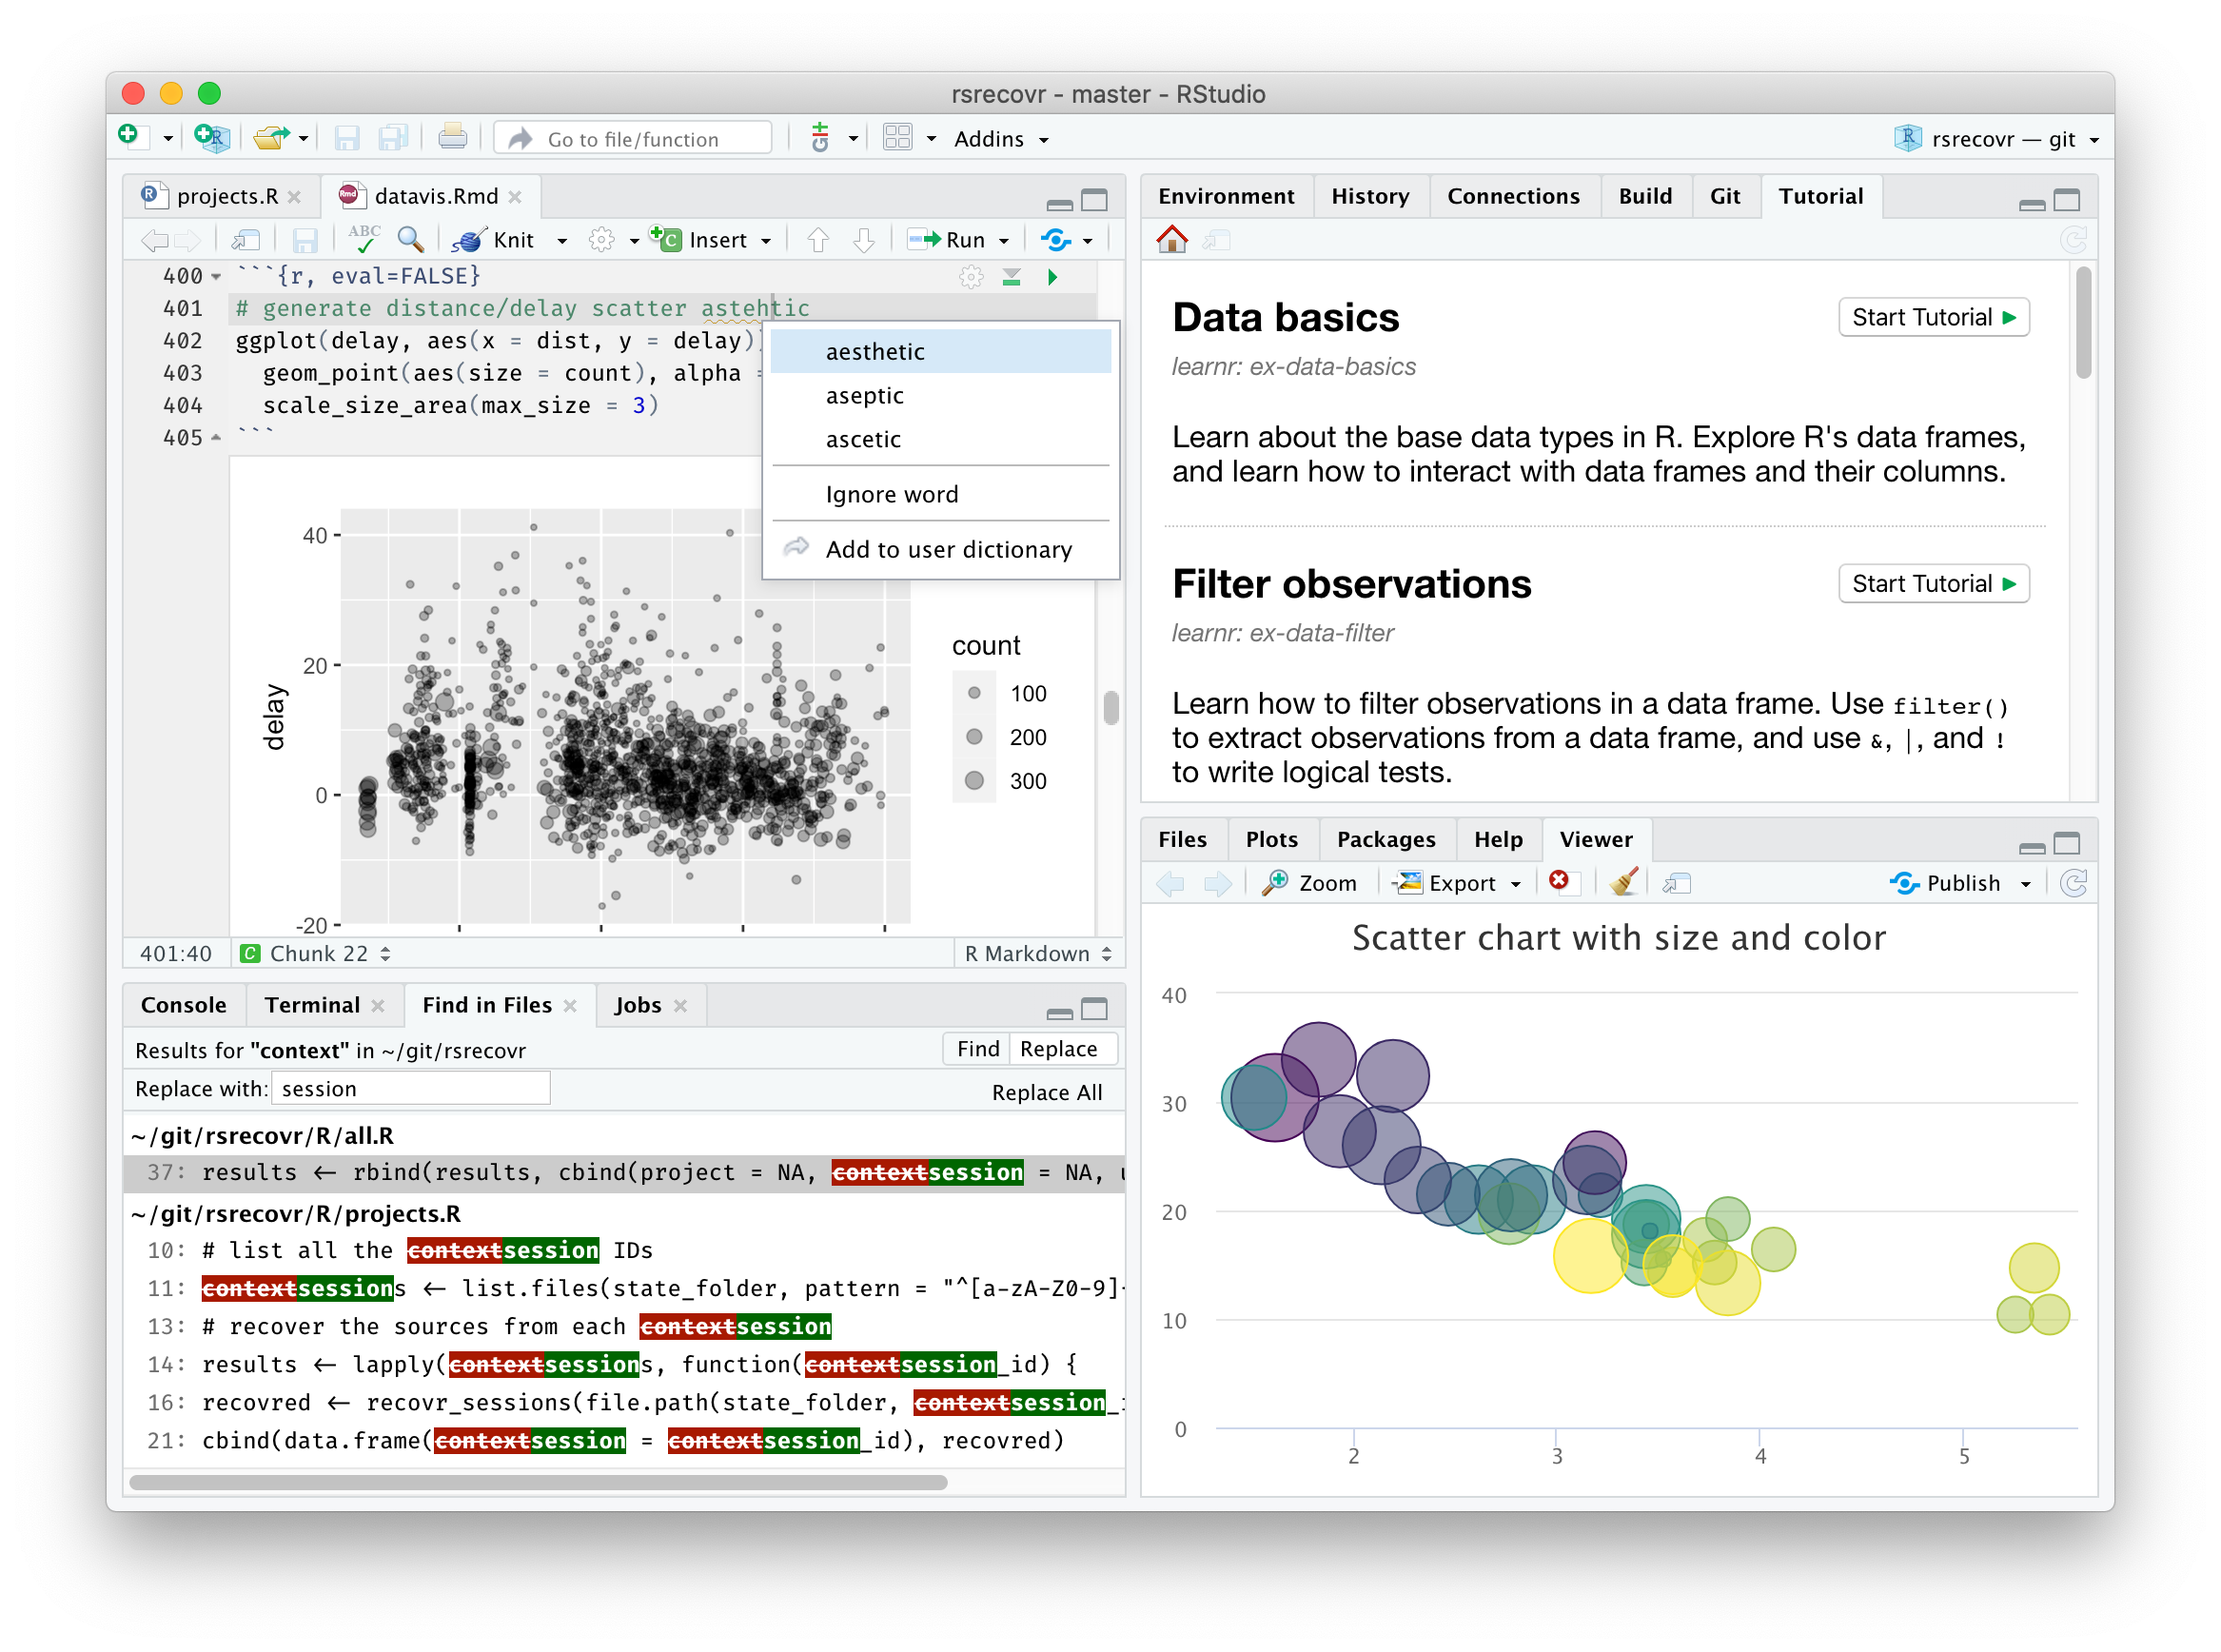
\includegraphics[width=8.33333in,height=\textheight,keepaspectratio]{img/rstudio.png}

}

\caption{Entorno de desarrollo RStudio}

\end{figure}%

\begin{itemize}
\tightlist
\item
  \href{https://rkward.kde.org}{RKWard}. Es otra otro de los entornos de
  desarrollo más completos que además incluye a posibilidad de añadir
  nuevos menús y cuadros de diálogo personalizados.
\end{itemize}

\begin{figure}[H]

{\centering 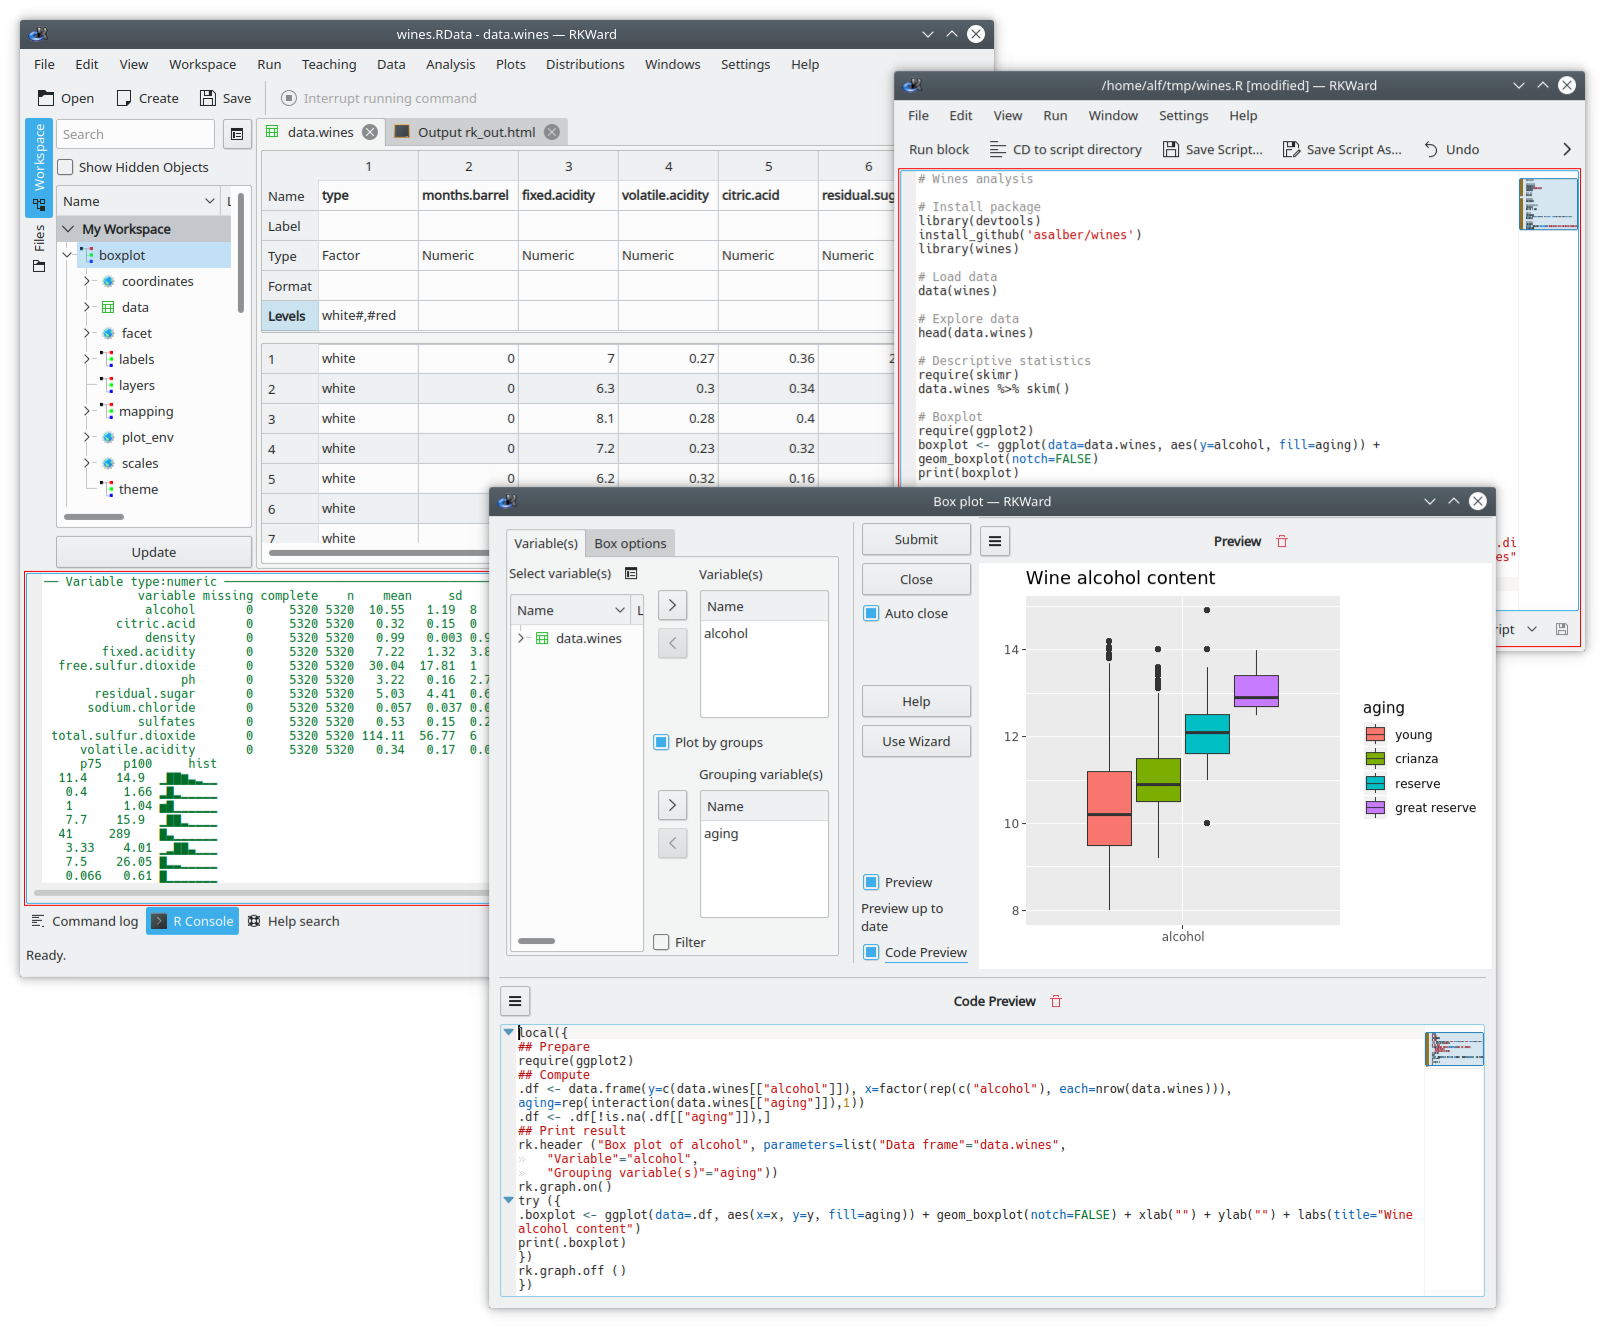
\includegraphics[width=8.33333in,height=\textheight,keepaspectratio]{img/rkward.png}

}

\caption{Entorno de desarrollo RKWard}

\end{figure}%

\begin{itemize}
\tightlist
\item
  \href{https://jupyter.org/}{Jupyter Lab}. Es un entorno de desarrollo
  interactivo que permite la creación de documentos que contienen
  código, texto, gráficos. Aunque no es un entorno de desarrollo
  específico para R, incluye un kernel para R que permite ejecutar
  código R en los documentos.
\end{itemize}

\begin{figure}[H]

{\centering 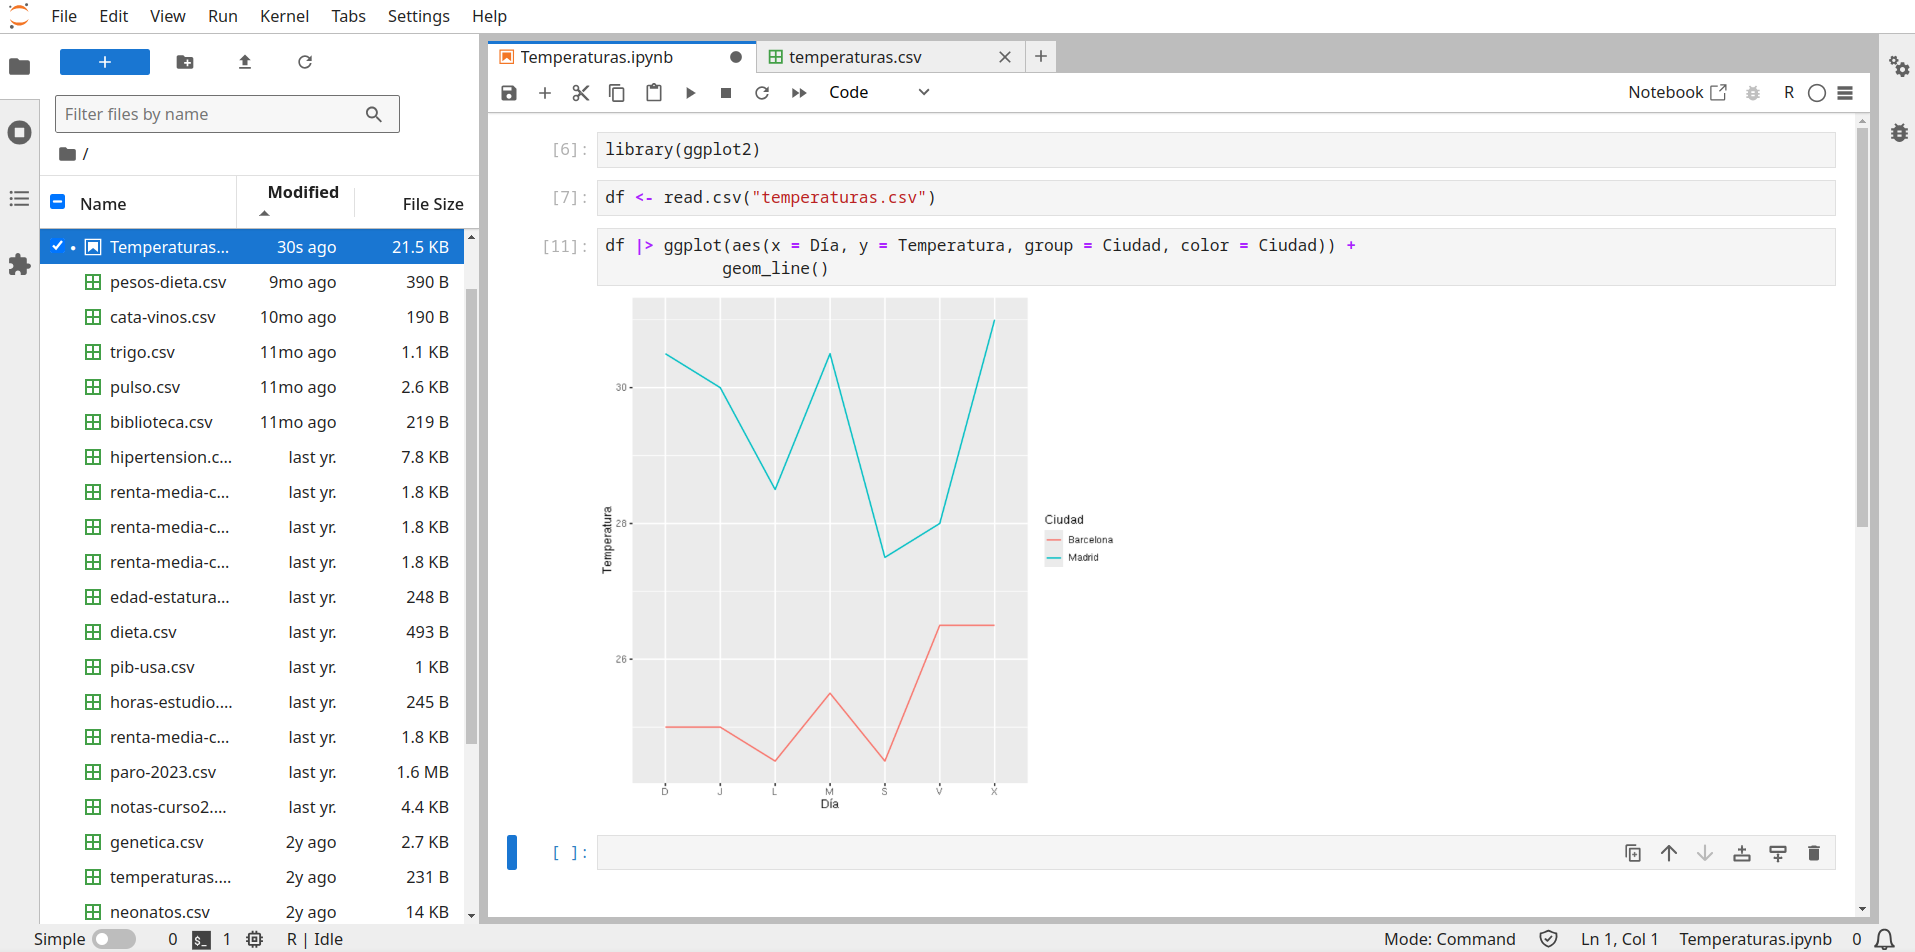
\includegraphics[width=8.33333in,height=\textheight,keepaspectratio]{img/jupyter-lab.png}

}

\caption{Entorno de desarrollo Jupyter Lab}

\end{figure}%

\begin{itemize}
\tightlist
\item
  \href{https://code.visualstudio.com/}{Visual Studio Code}. Es un
  entorno de desarrollo de propósito general ampliamente extendido.
  Aunque no es un entorno de desarrollo específico para R, incluye una
  extensión con utilidades que facilitan mucho el desarrollo con R.
\end{itemize}

\begin{figure}[H]

{\centering 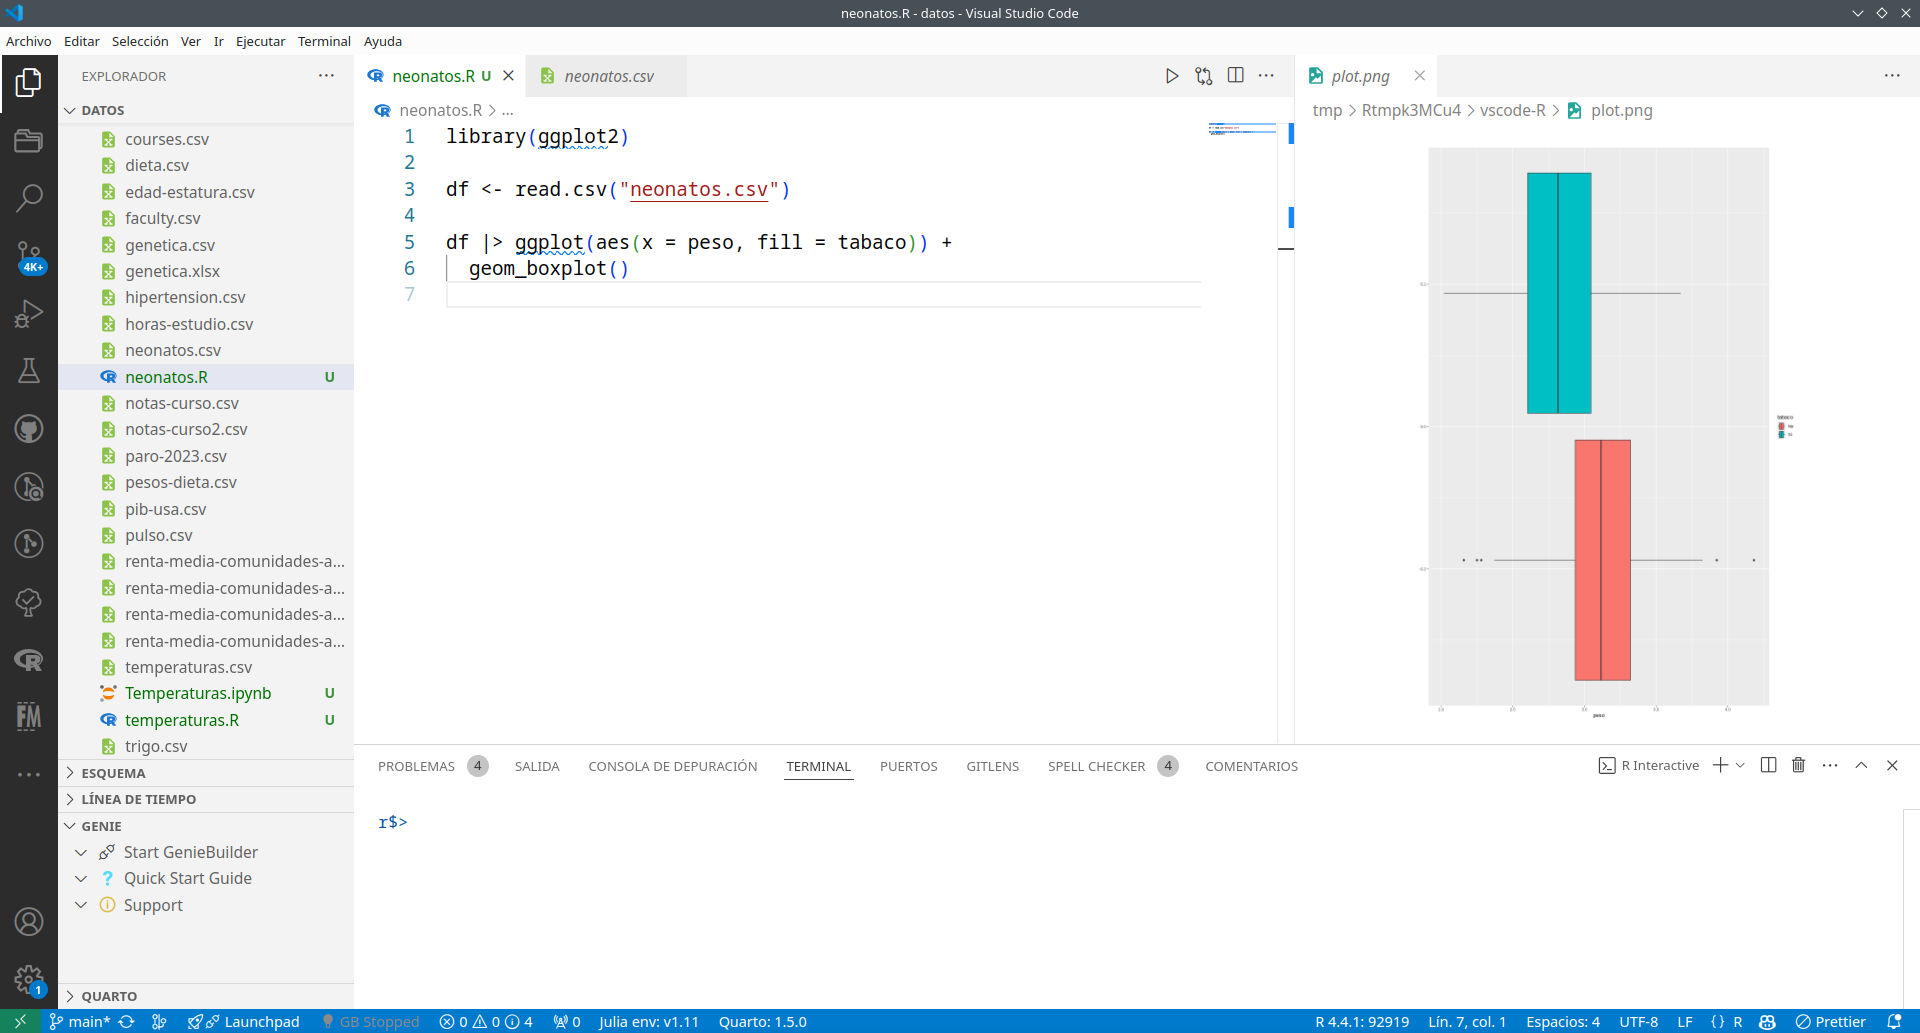
\includegraphics[width=8.33333in,height=\textheight,keepaspectratio]{img/vscode-r.png}

}

\caption{Entorno de desarrollo Visual Studio Code}

\end{figure}%

\section{Instalación de paquetes}\label{instalaciuxf3n-de-paquetes}

R es un lenguaje de programación modular, lo que significa que su
funcionalidad se extiende mediante paquetes. Los paquetes son
colecciones de funciones, datos y documentación sobre el uso de esas
funciones o conjuntos de datos.

El repositorio de paquetes más importante es
\href{https://cran.r-project.org/}{CRAN} (Comprehensive R Archive
Network), pero existen otros repositorios como
\href{https://www.bioconductor.org/}{Bioconductor} que contiene paquetes
específicos para el análisis de datos biológicos.

\subsection{Instalación de paquetes desde
CRAN}\label{instalaciuxf3n-de-paquetes-desde-cran}

Para instalar un paquete en R basta con ejecutar la función
\texttt{install.packages()} con el nombre del paquete que se desea
instalar. Por ejemplo, para instalar el paquete \texttt{ggplot2} que es
uno de los paquetes más utilizados para realizar gráficos en R, basta
con ejecutar el siguiente comando:

\begin{Shaded}
\begin{Highlighting}[]
\FunctionTok{install.packages}\NormalTok{(}\StringTok{"ggplot2"}\NormalTok{)}
\end{Highlighting}
\end{Shaded}

Los ubicación de los paquete instalados en R depende del sistema
operativo, pero puede consultarse en la variable \texttt{.libPaths()}.

\subsection{Instalación de paquetes desde
Bioconductor}\label{instalaciuxf3n-de-paquetes-desde-bioconductor}

Para instalar un paquete desde Bioconductor es necesario instalar
primero el paquete \texttt{BiocManager} y después utilizar la función
\texttt{BiocManager::install()} con el nombre del paquete que se desea
instalar. Por ejemplo, para instalar el paquete \texttt{DESeq2} que es
uno de los paquetes más utilizados para el análisis de datos de
expresión génica, basta con ejecutar el siguiente comando:

\begin{Shaded}
\begin{Highlighting}[]
\FunctionTok{install.packages}\NormalTok{(}\StringTok{"BiocManager"}\NormalTok{)}
\NormalTok{BiocManager}\SpecialCharTok{::}\FunctionTok{install}\NormalTok{(}\StringTok{"DESeq2"}\NormalTok{)}
\end{Highlighting}
\end{Shaded}

\section{Actualización de paquetes}\label{actualizaciuxf3n-de-paquetes}

Cada cierto tiempo conviene actualizar los paquetes instalados en R para
asegurarse de que se dispone de las últimas versiones de los mismos.
Para ello se puede utilizar la función \texttt{update.packages()}. Por
ejemplo, para actualizar todos los paquetes instalados en R sin
necesidad de confirmación por parte del usuario, basta con ejecutar el
siguiente comando:

\begin{Shaded}
\begin{Highlighting}[]
\FunctionTok{update.packages}\NormalTok{(}\AttributeTok{ask =} \ConstantTok{FALSE}\NormalTok{)}
\end{Highlighting}
\end{Shaded}

\bookmarksetup{startatroot}

\chapter{Tipos y estructuras de
datos}\label{tipos-y-estructuras-de-datos}

Esta práctica contiene ejercicios que muestran cómo trabajar con los
tipos y estructuras de datos en R. En concreto, las estructuras de datos
que se utilizan son

\begin{verbatim}
- Vectores.
- Factores.
- Matrices.
- Listas.
- Dataframes.
\end{verbatim}

\section{Ejercicios Resueltos}\label{ejercicios-resueltos}

Para la realización de esta práctica se requieren los siguientes
paquetes.

\begin{Shaded}
\begin{Highlighting}[]
\FunctionTok{library}\NormalTok{(tidyverse) }
\CommentTok{\# Incluye los siguientes paquetes:}
\CommentTok{\# {-} readr: para la lectura de ficheros csv. }
\CommentTok{\# {-} dplyr: para el preprocesamiento y manipulación de datos.}
\end{Highlighting}
\end{Shaded}

\begin{exercise}[]\protect\hypertarget{exr-vectores-1}{}\label{exr-vectores-1}

Realizar las siguientes operaciones con vectores.

\begin{enumerate}
\def\labelenumi{\alph{enumi}.}
\item
  Crear un vector con los números del 1 al 10.

  \begin{tcolorbox}[enhanced jigsaw, breakable, toptitle=1mm, colbacktitle=quarto-callout-tip-color!10!white, rightrule=.15mm, opacityback=0, opacitybacktitle=0.6, titlerule=0mm, coltitle=black, colframe=quarto-callout-tip-color-frame, colback=white, bottomtitle=1mm, leftrule=.75mm, toprule=.15mm, title=\textcolor{quarto-callout-tip-color}{\faLightbulb}\hspace{0.5em}{Solución}, arc=.35mm, bottomrule=.15mm, left=2mm]

  \section{Función c}

  La función \texttt{c()} permite combinar elementos en un vector. Los
  elementos se introducen separados por comas.

\begin{Shaded}
\begin{Highlighting}[]
\NormalTok{numeros }\OtherTok{\textless{}{-}} \FunctionTok{c}\NormalTok{(}\DecValTok{1}\NormalTok{, }\DecValTok{2}\NormalTok{, }\DecValTok{3}\NormalTok{, }\DecValTok{4}\NormalTok{, }\DecValTok{5}\NormalTok{, }\DecValTok{6}\NormalTok{, }\DecValTok{7}\NormalTok{, }\DecValTok{8}\NormalTok{, }\DecValTok{9}\NormalTok{, }\DecValTok{10}\NormalTok{)}
\NormalTok{numeros}
\end{Highlighting}
\end{Shaded}

\begin{verbatim}
 [1]  1  2  3  4  5  6  7  8  9 10
\end{verbatim}

  \section{Operador :}

  El operador \texttt{inicio:fin} permite crear un vector con la
  secuencia de números enteros desde el número \texttt{inicio} hasta el
  número \texttt{fin}.

\begin{Shaded}
\begin{Highlighting}[]
\NormalTok{numeros }\OtherTok{\textless{}{-}} \DecValTok{1}\SpecialCharTok{:}\DecValTok{10}
\NormalTok{numeros}
\end{Highlighting}
\end{Shaded}

\begin{verbatim}
 [1]  1  2  3  4  5  6  7  8  9 10
\end{verbatim}

  \end{tcolorbox}
\item
  Mostrar el número de elementos del vector anterior.

  \begin{tcolorbox}[enhanced jigsaw, breakable, toptitle=1mm, colbacktitle=quarto-callout-tip-color!10!white, rightrule=.15mm, opacityback=0, opacitybacktitle=0.6, titlerule=0mm, coltitle=black, colframe=quarto-callout-tip-color-frame, colback=white, bottomtitle=1mm, leftrule=.75mm, toprule=.15mm, title=\textcolor{quarto-callout-tip-color}{\faLightbulb}\hspace{0.5em}{Solución}, arc=.35mm, bottomrule=.15mm, left=2mm]

\begin{Shaded}
\begin{Highlighting}[]
\FunctionTok{length}\NormalTok{(numeros)}
\end{Highlighting}
\end{Shaded}

\begin{verbatim}
[1] 10
\end{verbatim}

  \end{tcolorbox}
\item
  Crear un vector con los números pares del 1 al 10.

  \begin{tcolorbox}[enhanced jigsaw, breakable, toptitle=1mm, colbacktitle=quarto-callout-tip-color!10!white, rightrule=.15mm, opacityback=0, opacitybacktitle=0.6, titlerule=0mm, coltitle=black, colframe=quarto-callout-tip-color-frame, colback=white, bottomtitle=1mm, leftrule=.75mm, toprule=.15mm, title=\textcolor{quarto-callout-tip-color}{\faLightbulb}\hspace{0.5em}{Solución}, arc=.35mm, bottomrule=.15mm, left=2mm]

  \section{Función c}

\begin{Shaded}
\begin{Highlighting}[]
\NormalTok{pares }\OtherTok{\textless{}{-}} \FunctionTok{c}\NormalTok{(}\DecValTok{2}\NormalTok{, }\DecValTok{4}\NormalTok{, }\DecValTok{6}\NormalTok{, }\DecValTok{8}\NormalTok{, }\DecValTok{10}\NormalTok{)}
\NormalTok{pares}
\end{Highlighting}
\end{Shaded}

\begin{verbatim}
[1]  2  4  6  8 10
\end{verbatim}

  \section{Función seq}

  La función \texttt{seq(inicio,\ fin,\ salto)} permite crear un vector
  con la secuencia de números enteros desde el número \texttt{inicio}
  hasta el número \texttt{fin} con un salto de \texttt{salto}.

\begin{Shaded}
\begin{Highlighting}[]
\NormalTok{pares }\OtherTok{\textless{}{-}} \FunctionTok{seq}\NormalTok{(}\DecValTok{2}\NormalTok{, }\DecValTok{10}\NormalTok{, }\AttributeTok{by =} \DecValTok{2}\NormalTok{)}
\NormalTok{pares}
\end{Highlighting}
\end{Shaded}

\begin{verbatim}
[1]  2  4  6  8 10
\end{verbatim}

  \end{tcolorbox}
\item
  Crear un vector con el cuadrado de los elementos del vector anterior.

  \begin{tcolorbox}[enhanced jigsaw, breakable, toptitle=1mm, colbacktitle=quarto-callout-tip-color!10!white, rightrule=.15mm, opacityback=0, opacitybacktitle=0.6, titlerule=0mm, coltitle=black, colframe=quarto-callout-tip-color-frame, colback=white, bottomtitle=1mm, leftrule=.75mm, toprule=.15mm, title=\textcolor{quarto-callout-tip-color}{\faLightbulb}\hspace{0.5em}{Solución}, arc=.35mm, bottomrule=.15mm, left=2mm]

  El operador \texttt{\^{}} permite elevar un número a otro. Cuando se
  aplica a un vector, eleva cada elemento del vector al número indicado.

\begin{Shaded}
\begin{Highlighting}[]
\NormalTok{cuadrados }\OtherTok{\textless{}{-}}\NormalTok{ pares}\SpecialCharTok{\^{}}\DecValTok{2}
\NormalTok{cuadrados}
\end{Highlighting}
\end{Shaded}

\begin{verbatim}
[1]   4  16  36  64 100
\end{verbatim}

  \end{tcolorbox}
\item
  Crear un vector con 5 números aleatorios entre 1 y 10.

  \begin{tcolorbox}[enhanced jigsaw, breakable, toptitle=1mm, colbacktitle=quarto-callout-tip-color!10!white, rightrule=.15mm, opacityback=0, opacitybacktitle=0.6, titlerule=0mm, coltitle=black, colframe=quarto-callout-tip-color-frame, colback=white, bottomtitle=1mm, leftrule=.75mm, toprule=.15mm, title=\textcolor{quarto-callout-tip-color}{\faLightbulb}\hspace{0.5em}{Solución}, arc=.35mm, bottomrule=.15mm, left=2mm]

  La función \texttt{sample(vector,\ n)} permite seleccionar \texttt{n}
  elementos aleatorios de \texttt{vector}. El muestreo es sin
  reemplazamiento.

\begin{Shaded}
\begin{Highlighting}[]
\NormalTok{aleatorios }\OtherTok{\textless{}{-}} \FunctionTok{sample}\NormalTok{(}\DecValTok{1}\SpecialCharTok{:}\DecValTok{10}\NormalTok{, }\DecValTok{5}\NormalTok{)}
\NormalTok{aleatorios}
\end{Highlighting}
\end{Shaded}

\begin{verbatim}
[1] 10  6  5  4  1
\end{verbatim}

  \end{tcolorbox}
\item
  Crear un vector booleano con los números del vector anterior que son
  pares.

  \begin{tcolorbox}[enhanced jigsaw, breakable, toptitle=1mm, colbacktitle=quarto-callout-tip-color!10!white, rightrule=.15mm, opacityback=0, opacitybacktitle=0.6, titlerule=0mm, coltitle=black, colframe=quarto-callout-tip-color-frame, colback=white, bottomtitle=1mm, leftrule=.75mm, toprule=.15mm, title=\textcolor{quarto-callout-tip-color}{\faLightbulb}\hspace{0.5em}{Solución}, arc=.35mm, bottomrule=.15mm, left=2mm]

  El operador \texttt{\%\%} permite calcular el resto de la división
  entera de dos números. Si el resto es 0, el número es par. Y el
  operador \texttt{==} permite comparar dos vectores elemento a
  elemento.

\begin{Shaded}
\begin{Highlighting}[]
\NormalTok{par }\OtherTok{\textless{}{-}}\NormalTok{ aleatorios }\SpecialCharTok{\%\%} \DecValTok{2} \SpecialCharTok{==} \DecValTok{0}
\NormalTok{par}
\end{Highlighting}
\end{Shaded}

\begin{verbatim}
[1]  TRUE  TRUE FALSE  TRUE FALSE
\end{verbatim}

  \end{tcolorbox}
\item
  Crear un vector con 100 números aleatorios entre 0 y 1.

  \begin{tcolorbox}[enhanced jigsaw, breakable, toptitle=1mm, colbacktitle=quarto-callout-tip-color!10!white, rightrule=.15mm, opacityback=0, opacitybacktitle=0.6, titlerule=0mm, coltitle=black, colframe=quarto-callout-tip-color-frame, colback=white, bottomtitle=1mm, leftrule=.75mm, toprule=.15mm, title=\textcolor{quarto-callout-tip-color}{\faLightbulb}\hspace{0.5em}{Solución}, arc=.35mm, bottomrule=.15mm, left=2mm]

  La función \texttt{runif(n,\ min,\ max)} permite generar \texttt{n}
  números aleatorios entre \texttt{min} y \texttt{max}.

\begin{Shaded}
\begin{Highlighting}[]
\NormalTok{aleatorios2 }\OtherTok{\textless{}{-}} \FunctionTok{runif}\NormalTok{(}\DecValTok{100}\NormalTok{, }\DecValTok{0}\NormalTok{, }\DecValTok{1}\NormalTok{)}
\NormalTok{aleatorios2}
\end{Highlighting}
\end{Shaded}

\begin{verbatim}
  [1] 0.66608376 0.51425114 0.69359129 0.54497484 0.28273358 0.92343348
  [7] 0.29231584 0.83729563 0.28622328 0.26682078 0.18672279 0.23222591
 [13] 0.31661245 0.30269337 0.15904600 0.03999592 0.21879954 0.81059855
 [19] 0.52569755 0.91465817 0.83134505 0.04577026 0.45609148 0.26518667
 [25] 0.30467220 0.50730687 0.18109621 0.75967064 0.20124804 0.25880982
 [31] 0.99215042 0.80735234 0.55333359 0.64640609 0.31182431 0.62181920
 [37] 0.32977018 0.50199747 0.67709453 0.48499124 0.24392883 0.76545979
 [43] 0.07377988 0.30968660 0.71727174 0.50454591 0.15299896 0.50393349
 [49] 0.49396092 0.75120020 0.17464982 0.84839241 0.86483383 0.04185728
 [55] 0.31718216 0.01374994 0.23902573 0.70649462 0.30809476 0.50854757
 [61] 0.05164662 0.56456984 0.12148019 0.89283638 0.01462726 0.78312110
 [67] 0.08996133 0.51918998 0.38426669 0.07005250 0.32064442 0.66849540
 [73] 0.92640048 0.47190972 0.14261534 0.54426976 0.19617465 0.89858049
 [79] 0.38949978 0.31087078 0.16002866 0.89618585 0.16639378 0.90042460
 [85] 0.13407820 0.13161413 0.10528750 0.51158358 0.30019905 0.02671690
 [91] 0.30964743 0.74211966 0.03545673 0.56507611 0.28025778 0.20419632
 [97] 0.13373890 0.32568192 0.15506197 0.12996214
\end{verbatim}

  \end{tcolorbox}
\item
  Ordenar el vector anterior de menor a mayor.

  \begin{tcolorbox}[enhanced jigsaw, breakable, toptitle=1mm, colbacktitle=quarto-callout-tip-color!10!white, rightrule=.15mm, opacityback=0, opacitybacktitle=0.6, titlerule=0mm, coltitle=black, colframe=quarto-callout-tip-color-frame, colback=white, bottomtitle=1mm, leftrule=.75mm, toprule=.15mm, title=\textcolor{quarto-callout-tip-color}{\faLightbulb}\hspace{0.5em}{Solución}, arc=.35mm, bottomrule=.15mm, left=2mm]

  La función \texttt{sort(vector)} permite ordenar los elementos de un
  vector de menor a mayor.

\begin{Shaded}
\begin{Highlighting}[]
\FunctionTok{sort}\NormalTok{(aleatorios2)}
\end{Highlighting}
\end{Shaded}

\begin{verbatim}
  [1] 0.01374994 0.01462726 0.02671690 0.03545673 0.03999592 0.04185728
  [7] 0.04577026 0.05164662 0.07005250 0.07377988 0.08996133 0.10528750
 [13] 0.12148019 0.12996214 0.13161413 0.13373890 0.13407820 0.14261534
 [19] 0.15299896 0.15506197 0.15904600 0.16002866 0.16639378 0.17464982
 [25] 0.18109621 0.18672279 0.19617465 0.20124804 0.20419632 0.21879954
 [31] 0.23222591 0.23902573 0.24392883 0.25880982 0.26518667 0.26682078
 [37] 0.28025778 0.28273358 0.28622328 0.29231584 0.30019905 0.30269337
 [43] 0.30467220 0.30809476 0.30964743 0.30968660 0.31087078 0.31182431
 [49] 0.31661245 0.31718216 0.32064442 0.32568192 0.32977018 0.38426669
 [55] 0.38949978 0.45609148 0.47190972 0.48499124 0.49396092 0.50199747
 [61] 0.50393349 0.50454591 0.50730687 0.50854757 0.51158358 0.51425114
 [67] 0.51918998 0.52569755 0.54426976 0.54497484 0.55333359 0.56456984
 [73] 0.56507611 0.62181920 0.64640609 0.66608376 0.66849540 0.67709453
 [79] 0.69359129 0.70649462 0.71727174 0.74211966 0.75120020 0.75967064
 [85] 0.76545979 0.78312110 0.80735234 0.81059855 0.83134505 0.83729563
 [91] 0.84839241 0.86483383 0.89283638 0.89618585 0.89858049 0.90042460
 [97] 0.91465817 0.92343348 0.92640048 0.99215042
\end{verbatim}

  \end{tcolorbox}
\item
  Ordenar el vector anterior de mayor a menor.

  \begin{tcolorbox}[enhanced jigsaw, breakable, toptitle=1mm, colbacktitle=quarto-callout-tip-color!10!white, rightrule=.15mm, opacityback=0, opacitybacktitle=0.6, titlerule=0mm, coltitle=black, colframe=quarto-callout-tip-color-frame, colback=white, bottomtitle=1mm, leftrule=.75mm, toprule=.15mm, title=\textcolor{quarto-callout-tip-color}{\faLightbulb}\hspace{0.5em}{Solución}, arc=.35mm, bottomrule=.15mm, left=2mm]

  La función \texttt{sort(vector,\ decreasing\ =\ TRUE)} permite ordenar
  los elementos de un vector de mayor a menor.

\begin{Shaded}
\begin{Highlighting}[]
\FunctionTok{sort}\NormalTok{(aleatorios2, }\AttributeTok{decreasing =} \ConstantTok{TRUE}\NormalTok{)}
\end{Highlighting}
\end{Shaded}

\begin{verbatim}
  [1] 0.99215042 0.92640048 0.92343348 0.91465817 0.90042460 0.89858049
  [7] 0.89618585 0.89283638 0.86483383 0.84839241 0.83729563 0.83134505
 [13] 0.81059855 0.80735234 0.78312110 0.76545979 0.75967064 0.75120020
 [19] 0.74211966 0.71727174 0.70649462 0.69359129 0.67709453 0.66849540
 [25] 0.66608376 0.64640609 0.62181920 0.56507611 0.56456984 0.55333359
 [31] 0.54497484 0.54426976 0.52569755 0.51918998 0.51425114 0.51158358
 [37] 0.50854757 0.50730687 0.50454591 0.50393349 0.50199747 0.49396092
 [43] 0.48499124 0.47190972 0.45609148 0.38949978 0.38426669 0.32977018
 [49] 0.32568192 0.32064442 0.31718216 0.31661245 0.31182431 0.31087078
 [55] 0.30968660 0.30964743 0.30809476 0.30467220 0.30269337 0.30019905
 [61] 0.29231584 0.28622328 0.28273358 0.28025778 0.26682078 0.26518667
 [67] 0.25880982 0.24392883 0.23902573 0.23222591 0.21879954 0.20419632
 [73] 0.20124804 0.19617465 0.18672279 0.18109621 0.17464982 0.16639378
 [79] 0.16002866 0.15904600 0.15506197 0.15299896 0.14261534 0.13407820
 [85] 0.13373890 0.13161413 0.12996214 0.12148019 0.10528750 0.08996133
 [91] 0.07377988 0.07005250 0.05164662 0.04577026 0.04185728 0.03999592
 [97] 0.03545673 0.02671690 0.01462726 0.01374994
\end{verbatim}

  \end{tcolorbox}
\item
  Crear un vector con los días laborables de la semana.

  \begin{tcolorbox}[enhanced jigsaw, breakable, toptitle=1mm, colbacktitle=quarto-callout-tip-color!10!white, rightrule=.15mm, opacityback=0, opacitybacktitle=0.6, titlerule=0mm, coltitle=black, colframe=quarto-callout-tip-color-frame, colback=white, bottomtitle=1mm, leftrule=.75mm, toprule=.15mm, title=\textcolor{quarto-callout-tip-color}{\faLightbulb}\hspace{0.5em}{Solución}, arc=.35mm, bottomrule=.15mm, left=2mm]

\begin{Shaded}
\begin{Highlighting}[]
\NormalTok{dias\_laborables }\OtherTok{\textless{}{-}} \FunctionTok{c}\NormalTok{(}\StringTok{"Lunes"}\NormalTok{, }\StringTok{"Martes"}\NormalTok{, }\StringTok{"Miércoles"}\NormalTok{, }\StringTok{"Jueves"}\NormalTok{, }\StringTok{"Viernes"}\NormalTok{)}
\NormalTok{dias\_laborables}
\end{Highlighting}
\end{Shaded}

\begin{verbatim}
[1] "Lunes"     "Martes"    "Miércoles" "Jueves"    "Viernes"  
\end{verbatim}

  \end{tcolorbox}
\item
  Añadir los días del fin de semana al vector anterior y guardar el
  resultado en una nueva variable.

  \begin{tcolorbox}[enhanced jigsaw, breakable, toptitle=1mm, colbacktitle=quarto-callout-tip-color!10!white, rightrule=.15mm, opacityback=0, opacitybacktitle=0.6, titlerule=0mm, coltitle=black, colframe=quarto-callout-tip-color-frame, colback=white, bottomtitle=1mm, leftrule=.75mm, toprule=.15mm, title=\textcolor{quarto-callout-tip-color}{\faLightbulb}\hspace{0.5em}{Solución}, arc=.35mm, bottomrule=.15mm, left=2mm]

\begin{Shaded}
\begin{Highlighting}[]
\NormalTok{dias }\OtherTok{\textless{}{-}} \FunctionTok{c}\NormalTok{(dias\_laborables, }\StringTok{"Sábado"}\NormalTok{, }\StringTok{"Domingo"}\NormalTok{)}
\NormalTok{dias}
\end{Highlighting}
\end{Shaded}

\begin{verbatim}
[1] "Lunes"     "Martes"    "Miércoles" "Jueves"    "Viernes"   "Sábado"   
[7] "Domingo"  
\end{verbatim}

  \end{tcolorbox}
\item
  Acceder al tercer elemento del vector.

  \begin{tcolorbox}[enhanced jigsaw, breakable, toptitle=1mm, colbacktitle=quarto-callout-tip-color!10!white, rightrule=.15mm, opacityback=0, opacitybacktitle=0.6, titlerule=0mm, coltitle=black, colframe=quarto-callout-tip-color-frame, colback=white, bottomtitle=1mm, leftrule=.75mm, toprule=.15mm, title=\textcolor{quarto-callout-tip-color}{\faLightbulb}\hspace{0.5em}{Solución}, arc=.35mm, bottomrule=.15mm, left=2mm]

\begin{Shaded}
\begin{Highlighting}[]
\NormalTok{dias\_laborables[}\DecValTok{3}\NormalTok{]}
\end{Highlighting}
\end{Shaded}

\begin{verbatim}
[1] "Miércoles"
\end{verbatim}

  \end{tcolorbox}
\item
  Seleccionar los días pares del vector.

  \begin{tcolorbox}[enhanced jigsaw, breakable, toptitle=1mm, colbacktitle=quarto-callout-tip-color!10!white, rightrule=.15mm, opacityback=0, opacitybacktitle=0.6, titlerule=0mm, coltitle=black, colframe=quarto-callout-tip-color-frame, colback=white, bottomtitle=1mm, leftrule=.75mm, toprule=.15mm, title=\textcolor{quarto-callout-tip-color}{\faLightbulb}\hspace{0.5em}{Solución}, arc=.35mm, bottomrule=.15mm, left=2mm]

  \section{Índices numéricos}

\begin{Shaded}
\begin{Highlighting}[]
\NormalTok{dias[}\FunctionTok{c}\NormalTok{(}\DecValTok{2}\NormalTok{, }\DecValTok{4}\NormalTok{, }\DecValTok{6}\NormalTok{)]}
\end{Highlighting}
\end{Shaded}

\begin{verbatim}
[1] "Martes" "Jueves" "Sábado"
\end{verbatim}

  \section{Índices numéricos negativos}

\begin{Shaded}
\begin{Highlighting}[]
\NormalTok{dias[}\SpecialCharTok{{-}}\FunctionTok{c}\NormalTok{(}\DecValTok{1}\NormalTok{, }\DecValTok{3}\NormalTok{, }\DecValTok{5}\NormalTok{, }\DecValTok{7}\NormalTok{)]}
\end{Highlighting}
\end{Shaded}

\begin{verbatim}
[1] "Martes" "Jueves" "Sábado"
\end{verbatim}

  \section{Índices lógicos}

\begin{Shaded}
\begin{Highlighting}[]
\NormalTok{dias[}\FunctionTok{c}\NormalTok{(}\ConstantTok{FALSE}\NormalTok{, }\ConstantTok{TRUE}\NormalTok{)]}
\end{Highlighting}
\end{Shaded}

\begin{verbatim}
[1] "Martes" "Jueves" "Sábado"
\end{verbatim}

  \end{tcolorbox}
\end{enumerate}

\end{exercise}

\begin{exercise}[]\protect\hypertarget{exr-factores-1}{}\label{exr-factores-1}

Se ha tomado una muestra de alumnos de una clase y se ha recogido la
información sobre el sexo de los alumnos obteniendo los siguientes
datos:

\[
\mbox{Mujer, Hombre, Mujer, Hombre, Mujer, Mujer, Hombre, Hombre}
\]

\begin{enumerate}
\def\labelenumi{\alph{enumi}.}
\item
  Crear un vector con los datos de la muestra.

  \begin{tcolorbox}[enhanced jigsaw, breakable, toptitle=1mm, colbacktitle=quarto-callout-tip-color!10!white, rightrule=.15mm, opacityback=0, opacitybacktitle=0.6, titlerule=0mm, coltitle=black, colframe=quarto-callout-tip-color-frame, colback=white, bottomtitle=1mm, leftrule=.75mm, toprule=.15mm, title=\textcolor{quarto-callout-tip-color}{\faLightbulb}\hspace{0.5em}{Solución}, arc=.35mm, bottomrule=.15mm, left=2mm]

\begin{Shaded}
\begin{Highlighting}[]
\NormalTok{sexo }\OtherTok{\textless{}{-}} \FunctionTok{c}\NormalTok{(}\StringTok{"Mujer"}\NormalTok{, }\StringTok{"Hombre"}\NormalTok{, }\StringTok{"Mujer"}\NormalTok{, }\StringTok{"Hombre"}\NormalTok{, }\StringTok{"Mujer"}\NormalTok{, }\StringTok{"Mujer"}\NormalTok{, }\StringTok{"Hombre"}\NormalTok{, }\StringTok{"Hombre"}\NormalTok{)}
\NormalTok{sexo}
\end{Highlighting}
\end{Shaded}

\begin{verbatim}
[1] "Mujer"  "Hombre" "Mujer"  "Hombre" "Mujer"  "Mujer"  "Hombre" "Hombre"
\end{verbatim}

  \end{tcolorbox}
\item
  Convertir el vector anterior en un factor.

  \begin{tcolorbox}[enhanced jigsaw, breakable, toptitle=1mm, colbacktitle=quarto-callout-tip-color!10!white, rightrule=.15mm, opacityback=0, opacitybacktitle=0.6, titlerule=0mm, coltitle=black, colframe=quarto-callout-tip-color-frame, colback=white, bottomtitle=1mm, leftrule=.75mm, toprule=.15mm, title=\textcolor{quarto-callout-tip-color}{\faLightbulb}\hspace{0.5em}{Solución}, arc=.35mm, bottomrule=.15mm, left=2mm]

  La función \texttt{factor(vector,\ labels)} permite convertir
  \texttt{vector} en un factor con los niveles o categorías
  especificados en \texttt{labels}. Si no se indica \texttt{labels}, los
  niveles se toman de los elementos del vector y se ordenan
  alfabéticamente.

\begin{Shaded}
\begin{Highlighting}[]
\NormalTok{sexo }\OtherTok{\textless{}{-}} \FunctionTok{factor}\NormalTok{(sexo)}
\NormalTok{sexo}
\end{Highlighting}
\end{Shaded}

\begin{verbatim}
[1] Mujer  Hombre Mujer  Hombre Mujer  Mujer  Hombre Hombre
Levels: Hombre Mujer
\end{verbatim}

  \end{tcolorbox}
\item
  Mostrar los niveles del factor.

  \begin{tcolorbox}[enhanced jigsaw, breakable, toptitle=1mm, colbacktitle=quarto-callout-tip-color!10!white, rightrule=.15mm, opacityback=0, opacitybacktitle=0.6, titlerule=0mm, coltitle=black, colframe=quarto-callout-tip-color-frame, colback=white, bottomtitle=1mm, leftrule=.75mm, toprule=.15mm, title=\textcolor{quarto-callout-tip-color}{\faLightbulb}\hspace{0.5em}{Solución}, arc=.35mm, bottomrule=.15mm, left=2mm]

  La función \texttt{levels(factor)} permite mostrar los niveles del
  factor \texttt{factor}.

\begin{Shaded}
\begin{Highlighting}[]
\FunctionTok{levels}\NormalTok{(sexo)}
\end{Highlighting}
\end{Shaded}

\begin{verbatim}
[1] "Hombre" "Mujer" 
\end{verbatim}

  \end{tcolorbox}
\item
  Reordenar los niveles del factor para que la categoría ``Mujer'' sea
  la primera.

  \begin{tcolorbox}[enhanced jigsaw, breakable, toptitle=1mm, colbacktitle=quarto-callout-tip-color!10!white, rightrule=.15mm, opacityback=0, opacitybacktitle=0.6, titlerule=0mm, coltitle=black, colframe=quarto-callout-tip-color-frame, colback=white, bottomtitle=1mm, leftrule=.75mm, toprule=.15mm, title=\textcolor{quarto-callout-tip-color}{\faLightbulb}\hspace{0.5em}{Solución}, arc=.35mm, bottomrule=.15mm, left=2mm]

\begin{Shaded}
\begin{Highlighting}[]
\NormalTok{sexo }\OtherTok{\textless{}{-}} \FunctionTok{factor}\NormalTok{(sexo, }\AttributeTok{levels =} \FunctionTok{c}\NormalTok{(}\StringTok{"Mujer"}\NormalTok{, }\StringTok{"Hombre"}\NormalTok{))}
\NormalTok{sexo}
\end{Highlighting}
\end{Shaded}

\begin{verbatim}
[1] Mujer  Hombre Mujer  Hombre Mujer  Mujer  Hombre Hombre
Levels: Mujer Hombre
\end{verbatim}

  \end{tcolorbox}
\end{enumerate}

\end{exercise}

\begin{exercise}[]\protect\hypertarget{exr-matrices-1}{}\label{exr-matrices-1}

Realizar las siguientes operaciones con matrices.

\begin{enumerate}
\def\labelenumi{\alph{enumi}.}
\item
  Crear una matriz de 2 filas y 2 columnas con los números del 1 al 4.

  \begin{tcolorbox}[enhanced jigsaw, breakable, toptitle=1mm, colbacktitle=quarto-callout-tip-color!10!white, rightrule=.15mm, opacityback=0, opacitybacktitle=0.6, titlerule=0mm, coltitle=black, colframe=quarto-callout-tip-color-frame, colback=white, bottomtitle=1mm, leftrule=.75mm, toprule=.15mm, title=\textcolor{quarto-callout-tip-color}{\faLightbulb}\hspace{0.5em}{Solución}, arc=.35mm, bottomrule=.15mm, left=2mm]

  La función \texttt{matrix(vector,\ nrow,\ ncol)} permite crear una
  matriz con los datos de \texttt{vector} el número de filas indicado en
  \texttt{nrow} y el número de columnas indicado en \texttt{ncol}.

\begin{Shaded}
\begin{Highlighting}[]
\NormalTok{A }\OtherTok{\textless{}{-}} \FunctionTok{matrix}\NormalTok{(}\DecValTok{1}\SpecialCharTok{:}\DecValTok{4}\NormalTok{, }\AttributeTok{nrow =} \DecValTok{2}\NormalTok{, }\AttributeTok{ncol =} \DecValTok{2}\NormalTok{)}
\NormalTok{A}
\end{Highlighting}
\end{Shaded}

\begin{verbatim}
     [,1] [,2]
[1,]    1    3
[2,]    2    4
\end{verbatim}

  \end{tcolorbox}
\item
  Añadir a la matriz anterior una nueva columna con los números del 5 y
  6.

  \begin{tcolorbox}[enhanced jigsaw, breakable, toptitle=1mm, colbacktitle=quarto-callout-tip-color!10!white, rightrule=.15mm, opacityback=0, opacitybacktitle=0.6, titlerule=0mm, coltitle=black, colframe=quarto-callout-tip-color-frame, colback=white, bottomtitle=1mm, leftrule=.75mm, toprule=.15mm, title=\textcolor{quarto-callout-tip-color}{\faLightbulb}\hspace{0.5em}{Solución}, arc=.35mm, bottomrule=.15mm, left=2mm]

  La función \texttt{cbind(matriz,\ vector)} permite añadir una nueva
  columna a la matriz \texttt{matriz} con los datos de \texttt{vector}.

\begin{Shaded}
\begin{Highlighting}[]
\NormalTok{A }\OtherTok{\textless{}{-}} \FunctionTok{cbind}\NormalTok{(A, }\DecValTok{5}\SpecialCharTok{:}\DecValTok{6}\NormalTok{)}
\NormalTok{A}
\end{Highlighting}
\end{Shaded}

\begin{verbatim}
     [,1] [,2] [,3]
[1,]    1    3    5
[2,]    2    4    6
\end{verbatim}

  \end{tcolorbox}
\item
  Crear una matriz de 2 filas y 2 columnas con los números del 1 al 4,
  rellenando los elementos por filas.

  \begin{tcolorbox}[enhanced jigsaw, breakable, toptitle=1mm, colbacktitle=quarto-callout-tip-color!10!white, rightrule=.15mm, opacityback=0, opacitybacktitle=0.6, titlerule=0mm, coltitle=black, colframe=quarto-callout-tip-color-frame, colback=white, bottomtitle=1mm, leftrule=.75mm, toprule=.15mm, title=\textcolor{quarto-callout-tip-color}{\faLightbulb}\hspace{0.5em}{Solución}, arc=.35mm, bottomrule=.15mm, left=2mm]

  La función \texttt{matrix} rellena los elementos de la matriz por
  columnas. Para rellenar los elementos por filas, se puede utilizar el
  parámetro opcional \texttt{byrow\ =\ TRUE}.

\begin{Shaded}
\begin{Highlighting}[]
\NormalTok{B }\OtherTok{\textless{}{-}} \FunctionTok{matrix}\NormalTok{(}\DecValTok{1}\SpecialCharTok{:}\DecValTok{4}\NormalTok{, }\AttributeTok{nrow =} \DecValTok{2}\NormalTok{, }\AttributeTok{ncol =} \DecValTok{2}\NormalTok{, }\AttributeTok{byrow =} \ConstantTok{TRUE}\NormalTok{)}
\NormalTok{B}
\end{Highlighting}
\end{Shaded}

\begin{verbatim}
     [,1] [,2]
[1,]    1    2
[2,]    3    4
\end{verbatim}

  \end{tcolorbox}
\item
  Crear otra matriz a partir de la anterior añadiendo una fila con los
  números 5 y 6.

  \begin{tcolorbox}[enhanced jigsaw, breakable, toptitle=1mm, colbacktitle=quarto-callout-tip-color!10!white, rightrule=.15mm, opacityback=0, opacitybacktitle=0.6, titlerule=0mm, coltitle=black, colframe=quarto-callout-tip-color-frame, colback=white, bottomtitle=1mm, leftrule=.75mm, toprule=.15mm, title=\textcolor{quarto-callout-tip-color}{\faLightbulb}\hspace{0.5em}{Solución}, arc=.35mm, bottomrule=.15mm, left=2mm]

\begin{Shaded}
\begin{Highlighting}[]
\NormalTok{B }\OtherTok{\textless{}{-}} \FunctionTok{rbind}\NormalTok{(B, }\DecValTok{5}\SpecialCharTok{:}\DecValTok{6}\NormalTok{)}
\NormalTok{B}
\end{Highlighting}
\end{Shaded}

\begin{verbatim}
     [,1] [,2]
[1,]    1    2
[2,]    3    4
[3,]    5    6
\end{verbatim}

  \end{tcolorbox}
\item
  Acceder al elemento de la segunda fila y la primera columna de la
  matriz anterior.

  \begin{tcolorbox}[enhanced jigsaw, breakable, toptitle=1mm, colbacktitle=quarto-callout-tip-color!10!white, rightrule=.15mm, opacityback=0, opacitybacktitle=0.6, titlerule=0mm, coltitle=black, colframe=quarto-callout-tip-color-frame, colback=white, bottomtitle=1mm, leftrule=.75mm, toprule=.15mm, title=\textcolor{quarto-callout-tip-color}{\faLightbulb}\hspace{0.5em}{Solución}, arc=.35mm, bottomrule=.15mm, left=2mm]

\begin{Shaded}
\begin{Highlighting}[]
\NormalTok{B[}\DecValTok{2}\NormalTok{, }\DecValTok{1}\NormalTok{]}
\end{Highlighting}
\end{Shaded}

\begin{verbatim}
[1] 3
\end{verbatim}

  \end{tcolorbox}
\item
  Seleccionar la primera fila de la matriz.

  \begin{tcolorbox}[enhanced jigsaw, breakable, toptitle=1mm, colbacktitle=quarto-callout-tip-color!10!white, rightrule=.15mm, opacityback=0, opacitybacktitle=0.6, titlerule=0mm, coltitle=black, colframe=quarto-callout-tip-color-frame, colback=white, bottomtitle=1mm, leftrule=.75mm, toprule=.15mm, title=\textcolor{quarto-callout-tip-color}{\faLightbulb}\hspace{0.5em}{Solución}, arc=.35mm, bottomrule=.15mm, left=2mm]

\begin{Shaded}
\begin{Highlighting}[]
\NormalTok{B[}\DecValTok{1}\NormalTok{, ]}
\end{Highlighting}
\end{Shaded}

\begin{verbatim}
[1] 1 2
\end{verbatim}

  \end{tcolorbox}
\item
  Seleccionar la segunda columna de la matriz.

  \begin{tcolorbox}[enhanced jigsaw, breakable, toptitle=1mm, colbacktitle=quarto-callout-tip-color!10!white, rightrule=.15mm, opacityback=0, opacitybacktitle=0.6, titlerule=0mm, coltitle=black, colframe=quarto-callout-tip-color-frame, colback=white, bottomtitle=1mm, leftrule=.75mm, toprule=.15mm, title=\textcolor{quarto-callout-tip-color}{\faLightbulb}\hspace{0.5em}{Solución}, arc=.35mm, bottomrule=.15mm, left=2mm]

\begin{Shaded}
\begin{Highlighting}[]
\NormalTok{B[, }\DecValTok{2}\NormalTok{]}
\end{Highlighting}
\end{Shaded}

\begin{verbatim}
[1] 2 4 6
\end{verbatim}

  \end{tcolorbox}
\item
  Multiplicar la matriz A por la matriz B.

  \begin{tcolorbox}[enhanced jigsaw, breakable, toptitle=1mm, colbacktitle=quarto-callout-tip-color!10!white, rightrule=.15mm, opacityback=0, opacitybacktitle=0.6, titlerule=0mm, coltitle=black, colframe=quarto-callout-tip-color-frame, colback=white, bottomtitle=1mm, leftrule=.75mm, toprule=.15mm, title=\textcolor{quarto-callout-tip-color}{\faLightbulb}\hspace{0.5em}{Solución}, arc=.35mm, bottomrule=.15mm, left=2mm]

  La multiplicación de matrices se realiza con el operador
  \texttt{\%*\%}.

\begin{Shaded}
\begin{Highlighting}[]
\NormalTok{A }\SpecialCharTok{\%*\%}\NormalTok{ B}
\end{Highlighting}
\end{Shaded}

\begin{verbatim}
     [,1] [,2]
[1,]   35   44
[2,]   44   56
\end{verbatim}

  \end{tcolorbox}
\item
  Calcular la transpuesta de la matriz A.

  \begin{tcolorbox}[enhanced jigsaw, breakable, toptitle=1mm, colbacktitle=quarto-callout-tip-color!10!white, rightrule=.15mm, opacityback=0, opacitybacktitle=0.6, titlerule=0mm, coltitle=black, colframe=quarto-callout-tip-color-frame, colback=white, bottomtitle=1mm, leftrule=.75mm, toprule=.15mm, title=\textcolor{quarto-callout-tip-color}{\faLightbulb}\hspace{0.5em}{Solución}, arc=.35mm, bottomrule=.15mm, left=2mm]

  La función \texttt{t(matriz)} permite calcular la transpuesta de
  \texttt{matriz}.

\begin{Shaded}
\begin{Highlighting}[]
\FunctionTok{t}\NormalTok{(A)}
\end{Highlighting}
\end{Shaded}

\begin{verbatim}
     [,1] [,2]
[1,]    1    2
[2,]    3    4
[3,]    5    6
\end{verbatim}

  \end{tcolorbox}
\end{enumerate}

\end{exercise}

\begin{exercise}[]\protect\hypertarget{exr-listas-1}{}\label{exr-listas-1}

Realizar las siguientes operaciones con listas.

\begin{enumerate}
\def\labelenumi{\alph{enumi}.}
\item
  Crear una lista con los siguientes con los datos del siguiente alumno:

  \begin{itemize}
  \tightlist
  \item
    Nombre: Juan.
  \item
    Edad: 20 años.
  \end{itemize}

  \begin{tcolorbox}[enhanced jigsaw, breakable, toptitle=1mm, colbacktitle=quarto-callout-tip-color!10!white, rightrule=.15mm, opacityback=0, opacitybacktitle=0.6, titlerule=0mm, coltitle=black, colframe=quarto-callout-tip-color-frame, colback=white, bottomtitle=1mm, leftrule=.75mm, toprule=.15mm, title=\textcolor{quarto-callout-tip-color}{\faLightbulb}\hspace{0.5em}{Solución}, arc=.35mm, bottomrule=.15mm, left=2mm]

  Para crear una lista se utiliza la función
  \texttt{list(nombre1\ =\ valor1,\ nombre2\ =\ valor2,\ ...)}.

\begin{Shaded}
\begin{Highlighting}[]
\NormalTok{alumno }\OtherTok{\textless{}{-}} \FunctionTok{list}\NormalTok{(}\AttributeTok{Nombre =} \StringTok{"Juan"}\NormalTok{, }\AttributeTok{Edad =} \DecValTok{20}\NormalTok{)}
\NormalTok{alumno}
\end{Highlighting}
\end{Shaded}

\begin{verbatim}
$Nombre
[1] "Juan"

$Edad
[1] 20
\end{verbatim}

  \end{tcolorbox}
\item
  Obtener la edad del alumno.

  \begin{tcolorbox}[enhanced jigsaw, breakable, toptitle=1mm, colbacktitle=quarto-callout-tip-color!10!white, rightrule=.15mm, opacityback=0, opacitybacktitle=0.6, titlerule=0mm, coltitle=black, colframe=quarto-callout-tip-color-frame, colback=white, bottomtitle=1mm, leftrule=.75mm, toprule=.15mm, title=\textcolor{quarto-callout-tip-color}{\faLightbulb}\hspace{0.5em}{Solución}, arc=.35mm, bottomrule=.15mm, left=2mm]

  Para acceder a los elementos de una lista se utiliza el operador
  \texttt{\$}.

\begin{Shaded}
\begin{Highlighting}[]
\NormalTok{alumno}\SpecialCharTok{$}\NormalTok{Edad}
\end{Highlighting}
\end{Shaded}

\begin{verbatim}
[1] 20
\end{verbatim}

  \end{tcolorbox}
\item
  Crear una lista con las siguientes notas del alumno:

  \begin{itemize}
  \tightlist
  \item
    Matemáticas: 7.
  \item
    Química: 8.
  \end{itemize}

  \begin{tcolorbox}[enhanced jigsaw, breakable, toptitle=1mm, colbacktitle=quarto-callout-tip-color!10!white, rightrule=.15mm, opacityback=0, opacitybacktitle=0.6, titlerule=0mm, coltitle=black, colframe=quarto-callout-tip-color-frame, colback=white, bottomtitle=1mm, leftrule=.75mm, toprule=.15mm, title=\textcolor{quarto-callout-tip-color}{\faLightbulb}\hspace{0.5em}{Solución}, arc=.35mm, bottomrule=.15mm, left=2mm]

\begin{Shaded}
\begin{Highlighting}[]
\NormalTok{notas }\OtherTok{\textless{}{-}} \FunctionTok{list}\NormalTok{(Matemáticas }\OtherTok{=} \DecValTok{7}\NormalTok{, Química }\OtherTok{=} \DecValTok{8}\NormalTok{)}
\NormalTok{notas}
\end{Highlighting}
\end{Shaded}

\begin{verbatim}
$Matemáticas
[1] 7

$Química
[1] 8
\end{verbatim}

  \end{tcolorbox}
\item
  Añadir la lista de notas a la lista del alumno.

  \begin{tcolorbox}[enhanced jigsaw, breakable, toptitle=1mm, colbacktitle=quarto-callout-tip-color!10!white, rightrule=.15mm, opacityback=0, opacitybacktitle=0.6, titlerule=0mm, coltitle=black, colframe=quarto-callout-tip-color-frame, colback=white, bottomtitle=1mm, leftrule=.75mm, toprule=.15mm, title=\textcolor{quarto-callout-tip-color}{\faLightbulb}\hspace{0.5em}{Solución}, arc=.35mm, bottomrule=.15mm, left=2mm]

\begin{Shaded}
\begin{Highlighting}[]
\NormalTok{alumno}\SpecialCharTok{$}\NormalTok{Notas }\OtherTok{\textless{}{-}}\NormalTok{ notas}
\NormalTok{alumno}
\end{Highlighting}
\end{Shaded}

\begin{verbatim}
$Nombre
[1] "Juan"

$Edad
[1] 20

$Notas
$Notas$Matemáticas
[1] 7

$Notas$Química
[1] 8
\end{verbatim}

  \end{tcolorbox}
\item
  Añadir a la lista anterior la nota del examen de Física, que ha sido
  un 6.

  \begin{tcolorbox}[enhanced jigsaw, breakable, toptitle=1mm, colbacktitle=quarto-callout-tip-color!10!white, rightrule=.15mm, opacityback=0, opacitybacktitle=0.6, titlerule=0mm, coltitle=black, colframe=quarto-callout-tip-color-frame, colback=white, bottomtitle=1mm, leftrule=.75mm, toprule=.15mm, title=\textcolor{quarto-callout-tip-color}{\faLightbulb}\hspace{0.5em}{Solución}, arc=.35mm, bottomrule=.15mm, left=2mm]

\begin{Shaded}
\begin{Highlighting}[]
\NormalTok{alumno}\SpecialCharTok{$}\NormalTok{Notas}\SpecialCharTok{$}\NormalTok{Física }\OtherTok{\textless{}{-}} \DecValTok{6}
\NormalTok{alumno}
\end{Highlighting}
\end{Shaded}

\begin{verbatim}
$Nombre
[1] "Juan"

$Edad
[1] 20

$Notas
$Notas$Matemáticas
[1] 7

$Notas$Química
[1] 8

$Notas$Física
[1] 6
\end{verbatim}

  \end{tcolorbox}
\end{enumerate}

\end{exercise}

\begin{exercise}[]\protect\hypertarget{exr-dataframes-1}{}\label{exr-dataframes-1}

La siguiente tabla contiene los ingresos y gastos de una empresa durante
el primer trimestre del año.

\begin{longtable}[]{@{}lrrr@{}}
\toprule\noalign{}
Mes & Ingresos & Gastos & Impuestos \\
\midrule\noalign{}
\endhead
\bottomrule\noalign{}
\endlastfoot
Enero & 45000 & 33400 & 6450 \\
Febrero & 41500 & 35400 & 6300 \\
Marzo & 51200 & 35600 & 7100 \\
\end{longtable}

\begin{enumerate}
\def\labelenumi{\alph{enumi}.}
\item
  Crear un data frame con los datos de la tabla.

  \begin{tcolorbox}[enhanced jigsaw, breakable, toptitle=1mm, colbacktitle=quarto-callout-tip-color!10!white, rightrule=.15mm, opacityback=0, opacitybacktitle=0.6, titlerule=0mm, coltitle=black, colframe=quarto-callout-tip-color-frame, colback=white, bottomtitle=1mm, leftrule=.75mm, toprule=.15mm, title=\textcolor{quarto-callout-tip-color}{\faLightbulb}\hspace{0.5em}{Solución}, arc=.35mm, bottomrule=.15mm, left=2mm]

  Para crear un data frame se utiliza la función
  \texttt{data.frame(columna1\ =\ vector1,\ columna2\ =\ vector2,\ ...)},
  donde \texttt{columna1}, \texttt{columna2}, \ldots{} son los nombres
  de las columnas y \texttt{vector1}, \texttt{vector2}, \ldots{} son los
  vectores con los datos de cada columna, que deben tener la misma
  longitud.

\begin{Shaded}
\begin{Highlighting}[]
\NormalTok{df }\OtherTok{\textless{}{-}} \FunctionTok{data.frame}\NormalTok{(}
    \AttributeTok{Mes =} \FunctionTok{c}\NormalTok{(}\StringTok{"Enero"}\NormalTok{, }\StringTok{"Febrero"}\NormalTok{, }\StringTok{"Marzo"}\NormalTok{),}
    \AttributeTok{Ingresos =} \FunctionTok{c}\NormalTok{(}\DecValTok{45000}\NormalTok{, }\DecValTok{41500}\NormalTok{, }\DecValTok{51200}\NormalTok{),}
    \AttributeTok{Gastos =} \FunctionTok{c}\NormalTok{(}\DecValTok{33400}\NormalTok{, }\DecValTok{35400}\NormalTok{, }\DecValTok{35600}\NormalTok{)}
\NormalTok{    )}
\NormalTok{df }
\end{Highlighting}
\end{Shaded}

\begin{verbatim}
      Mes Ingresos Gastos
1   Enero    45000  33400
2 Febrero    41500  35400
3   Marzo    51200  35600
\end{verbatim}

  \end{tcolorbox}
\item
  Añadir una nueva columna con los siguientes impuestos pagados.

  \begin{longtable*}[t]{lr}
  \toprule
  Mes & Impuestos\\
  \midrule
  Enero & 6450\\
  Febrero & 6300\\
  Marzo & 7100\\
  \bottomrule
  \end{longtable*}

  \begin{tcolorbox}[enhanced jigsaw, breakable, toptitle=1mm, colbacktitle=quarto-callout-tip-color!10!white, rightrule=.15mm, opacityback=0, opacitybacktitle=0.6, titlerule=0mm, coltitle=black, colframe=quarto-callout-tip-color-frame, colback=white, bottomtitle=1mm, leftrule=.75mm, toprule=.15mm, title=\textcolor{quarto-callout-tip-color}{\faLightbulb}\hspace{0.5em}{Solución}, arc=.35mm, bottomrule=.15mm, left=2mm]

  \section{Base}

  Con las funciones del paquete \texttt{base} de R.

\begin{Shaded}
\begin{Highlighting}[]
\NormalTok{df}\SpecialCharTok{$}\NormalTok{Impuestos }\OtherTok{\textless{}{-}} \FunctionTok{c}\NormalTok{(}\DecValTok{6450}\NormalTok{, }\DecValTok{6300}\NormalTok{, }\DecValTok{7100}\NormalTok{)}
\NormalTok{df}
\end{Highlighting}
\end{Shaded}

\begin{verbatim}
      Mes Ingresos Gastos Impuestos
1   Enero    45000  33400      6450
2 Febrero    41500  35400      6300
3   Marzo    51200  35600      7100
\end{verbatim}

  \section{Tidyverse}

  Con las funciones del paquete \texttt{dplyr} de \texttt{tidyverse}.

\begin{Shaded}
\begin{Highlighting}[]
\NormalTok{df }\OtherTok{\textless{}{-}}\NormalTok{ df }\SpecialCharTok{|\textgreater{}} \FunctionTok{mutate}\NormalTok{(}\AttributeTok{Impuestos =} \FunctionTok{c}\NormalTok{(}\DecValTok{6450}\NormalTok{, }\DecValTok{6300}\NormalTok{, }\DecValTok{7100}\NormalTok{))}
\NormalTok{df}
\end{Highlighting}
\end{Shaded}

\begin{verbatim}
      Mes Ingresos Gastos Impuestos
1   Enero    45000  33400      6450
2 Febrero    41500  35400      6300
3   Marzo    51200  35600      7100
\end{verbatim}

  \end{tcolorbox}
\item
  Añadir una nueva fila con los siguientes datos de Abril.

  \begin{longtable}[]{@{}lrrr@{}}
  \toprule\noalign{}
  Mes & Ingresos & Gastos & Impuestos \\
  \midrule\noalign{}
  \endhead
  \bottomrule\noalign{}
  \endlastfoot
  Abril & 49700 & 36300 & 6850 \\
  \end{longtable}

  \begin{tcolorbox}[enhanced jigsaw, breakable, toptitle=1mm, colbacktitle=quarto-callout-tip-color!10!white, rightrule=.15mm, opacityback=0, opacitybacktitle=0.6, titlerule=0mm, coltitle=black, colframe=quarto-callout-tip-color-frame, colback=white, bottomtitle=1mm, leftrule=.75mm, toprule=.15mm, title=\textcolor{quarto-callout-tip-color}{\faLightbulb}\hspace{0.5em}{Solución}, arc=.35mm, bottomrule=.15mm, left=2mm]

  \section{Base}

  Con las funciones del paquete \texttt{base} de R.

\begin{Shaded}
\begin{Highlighting}[]
\NormalTok{df }\OtherTok{\textless{}{-}} \FunctionTok{rbind}\NormalTok{(df, }\FunctionTok{list}\NormalTok{(}\AttributeTok{Mes =} \StringTok{"Abril"}\NormalTok{, }\AttributeTok{Ingresos =} \DecValTok{49700}\NormalTok{, }\AttributeTok{Gastos =} \DecValTok{36300}\NormalTok{, }\AttributeTok{Impuestos =} \DecValTok{6850}\NormalTok{))}
\NormalTok{df}
\end{Highlighting}
\end{Shaded}

\begin{verbatim}
      Mes Ingresos Gastos Impuestos
1   Enero    45000  33400      6450
2 Febrero    41500  35400      6300
3   Marzo    51200  35600      7100
4   Abril    49700  36300      6850
\end{verbatim}

  \section{Tidyverse}

  Con las funciones del paquete \texttt{dplyr} de \texttt{tidyverse}.

\begin{Shaded}
\begin{Highlighting}[]
\NormalTok{df }\OtherTok{\textless{}{-}}\NormalTok{ df }\SpecialCharTok{|\textgreater{}} \FunctionTok{add\_row}\NormalTok{(}\AttributeTok{Mes =} \StringTok{"Abril"}\NormalTok{, }\AttributeTok{Ingresos =} \DecValTok{49700}\NormalTok{, }\AttributeTok{Gastos =} \DecValTok{36300}\NormalTok{, }\AttributeTok{Impuestos =} \DecValTok{6850}\NormalTok{)}
\NormalTok{df}
\end{Highlighting}
\end{Shaded}

\begin{verbatim}
      Mes Ingresos Gastos Impuestos
1   Enero    45000  33400      6450
2 Febrero    41500  35400      6300
3   Marzo    51200  35600      7100
4   Abril    49700  36300      6850
\end{verbatim}

  \end{tcolorbox}
\item
  Cambiar los ingresos de Marzo por 50400.

  \begin{tcolorbox}[enhanced jigsaw, breakable, toptitle=1mm, colbacktitle=quarto-callout-tip-color!10!white, rightrule=.15mm, opacityback=0, opacitybacktitle=0.6, titlerule=0mm, coltitle=black, colframe=quarto-callout-tip-color-frame, colback=white, bottomtitle=1mm, leftrule=.75mm, toprule=.15mm, title=\textcolor{quarto-callout-tip-color}{\faLightbulb}\hspace{0.5em}{Solución}, arc=.35mm, bottomrule=.15mm, left=2mm]

\begin{Shaded}
\begin{Highlighting}[]
\NormalTok{df[}\DecValTok{3}\NormalTok{, }\StringTok{"Ingresos"}\NormalTok{] }\OtherTok{\textless{}{-}} \DecValTok{50400}
\NormalTok{df}
\end{Highlighting}
\end{Shaded}

\begin{verbatim}
      Mes Ingresos Gastos Impuestos
1   Enero    45000  33400      6450
2 Febrero    41500  35400      6300
3   Marzo    50400  35600      7100
4   Abril    49700  36300      6850
\end{verbatim}

  \end{tcolorbox}
\item
  Guardar el data frame en un fichero csv.

  \begin{tcolorbox}[enhanced jigsaw, breakable, toptitle=1mm, colbacktitle=quarto-callout-tip-color!10!white, rightrule=.15mm, opacityback=0, opacitybacktitle=0.6, titlerule=0mm, coltitle=black, colframe=quarto-callout-tip-color-frame, colback=white, bottomtitle=1mm, leftrule=.75mm, toprule=.15mm, title=\textcolor{quarto-callout-tip-color}{\faLightbulb}\hspace{0.5em}{Solución}, arc=.35mm, bottomrule=.15mm, left=2mm]

  La función \texttt{write.csv(dataframe,\ "fichero.csv")} permite
  guardar el data frame \texttt{dataframe} en el fichero
  \texttt{fichero.csv}.

\begin{Shaded}
\begin{Highlighting}[]
\FunctionTok{write.csv}\NormalTok{(df, }\StringTok{"datos/ingresos\_gastos.csv"}\NormalTok{, }\AttributeTok{row.names =} \ConstantTok{FALSE}\NormalTok{)}
\end{Highlighting}
\end{Shaded}

  \end{tcolorbox}
\end{enumerate}

\end{exercise}

\begin{exercise}[]\protect\hypertarget{exr-dataframes-2}{}\label{exr-dataframes-2}

El fichero \href{datos/colesterol.csv}{\texttt{colesterol.csv}} contiene
información de una muestra de pacientes donde se han medido la edad, el
sexo, el peso, la altura y el nivel de colesterol, además de su nombre.

\begin{enumerate}
\def\labelenumi{\alph{enumi}.}
\item
  Crear un data frame con los datos de todos los pacientes del estudio a
  partir del fichero
  \href{datos/colesterol.csv}{\texttt{colesterol.csv}} y mostrar las
  primeras filas.

  \begin{tcolorbox}[enhanced jigsaw, breakable, toptitle=1mm, colbacktitle=quarto-callout-tip-color!10!white, rightrule=.15mm, opacityback=0, opacitybacktitle=0.6, titlerule=0mm, coltitle=black, colframe=quarto-callout-tip-color-frame, colback=white, bottomtitle=1mm, leftrule=.75mm, toprule=.15mm, title=\textcolor{quarto-callout-tip-color}{\faLightbulb}\hspace{0.5em}{Solución}, arc=.35mm, bottomrule=.15mm, left=2mm]

  \section{Base}

  Con las funciones del paquete \texttt{base} de R. La función
  \texttt{read.csv("fichero.csv")} permite leer un fichero csv y cargar
  los datos en un data frame. Y la función \texttt{head(dataframe)}
  permite mostrar las primeras filas del data frame \texttt{dataframe}.

\begin{Shaded}
\begin{Highlighting}[]
\NormalTok{df }\OtherTok{\textless{}{-}} \FunctionTok{read.csv}\NormalTok{(}\StringTok{"https://aprendeconalf.es/estadistica{-}practicas{-}r/datos/colesterol.csv"}\NormalTok{)}
\FunctionTok{head}\NormalTok{(df)}
\end{Highlighting}
\end{Shaded}

\begin{verbatim}
                        nombre edad sexo peso altura colesterol
1 José Luis Martínez Izquierdo   18    H   85   1.79        182
2               Rosa Díaz Díaz   32    M   65   1.73        232
3        Javier García Sánchez   24    H   NA   1.81        191
4          Carmen López Pinzón   35    M   65   1.70        200
5         Marisa López Collado   46    M   51   1.58        148
6            Antonio Ruiz Cruz   68    H   66   1.74        249
\end{verbatim}

  \section{Tidyverse}

  Con la función
  \href{https://readr.tidyverse.org/reference/read_delim.html}{\texttt{read\_csv}}
  del paquete del paquete
  \href{https://readr.tidyverse.org/index.html}{\texttt{readr}} de
  \texttt{tidyverse}.

\begin{Shaded}
\begin{Highlighting}[]
\NormalTok{df }\OtherTok{\textless{}{-}} \FunctionTok{read\_csv}\NormalTok{(}\StringTok{"https://aprendeconalf.es/estadistica{-}practicas{-}r/datos/colesterol.csv"}\NormalTok{)}
\end{Highlighting}
\end{Shaded}

\begin{verbatim}
Rows: 14 Columns: 6
-- Column specification --------------------------------------------------------
Delimiter: ","
chr (2): nombre, sexo
dbl (4): edad, peso, altura, colesterol

i Use `spec()` to retrieve the full column specification for this data.
i Specify the column types or set `show_col_types = FALSE` to quiet this message.
\end{verbatim}

\begin{Shaded}
\begin{Highlighting}[]
\FunctionTok{head}\NormalTok{(df)}
\end{Highlighting}
\end{Shaded}

\begin{verbatim}
# A tibble: 6 x 6
  nombre                        edad sexo   peso altura colesterol
  <chr>                        <dbl> <chr> <dbl>  <dbl>      <dbl>
1 José Luis Martínez Izquierdo    18 H        85   1.79        182
2 Rosa Díaz Díaz                  32 M        65   1.73        232
3 Javier García Sánchez           24 H        NA   1.81        191
4 Carmen López Pinzón             35 M        65   1.7         200
5 Marisa López Collado            46 M        51   1.58        148
6 Antonio Ruiz Cruz               68 H        66   1.74        249
\end{verbatim}

  \end{tcolorbox}
\item
  Mostrar las variables del data frame.

  \begin{tcolorbox}[enhanced jigsaw, breakable, toptitle=1mm, colbacktitle=quarto-callout-tip-color!10!white, rightrule=.15mm, opacityback=0, opacitybacktitle=0.6, titlerule=0mm, coltitle=black, colframe=quarto-callout-tip-color-frame, colback=white, bottomtitle=1mm, leftrule=.75mm, toprule=.15mm, title=\textcolor{quarto-callout-tip-color}{\faLightbulb}\hspace{0.5em}{Solución}, arc=.35mm, bottomrule=.15mm, left=2mm]

  \section{Base}

  Con las funciones del paquete \texttt{base} de R.

\begin{Shaded}
\begin{Highlighting}[]
\FunctionTok{colnames}\NormalTok{(df)}
\end{Highlighting}
\end{Shaded}

\begin{verbatim}
[1] "nombre"     "edad"       "sexo"       "peso"       "altura"    
[6] "colesterol"
\end{verbatim}

  \section{Tidyverse}

  Con la función
  \href{https://dplyr.tidyverse.org/reference/glimpse.html?q=read_csv\#undefined}{\texttt{glimpse}}
  del paquete
  \href{https://dplyr.tidyverse.org/index.html}{\texttt{dplyr}} de
  \texttt{tidyverse}. Esta función muestra las columnas del data frame
  en filas, de manera que permite ver todas las columnas de un data
  frame cuando este tiene muchas columnas.

\begin{Shaded}
\begin{Highlighting}[]
\FunctionTok{glimpse}\NormalTok{(df)}
\end{Highlighting}
\end{Shaded}

\begin{verbatim}
Rows: 14
Columns: 6
$ nombre     <chr> "José Luis Martínez Izquierdo", "Rosa Díaz Díaz", "Javier G~
$ edad       <dbl> 18, 32, 24, 35, 46, 68, 51, 22, 35, 46, 53, 58, 27, 20
$ sexo       <chr> "H", "M", "H", "M", "M", "H", "H", "M", "H", "H", "M", "H",~
$ peso       <dbl> 85, 65, NA, 65, 51, 66, 62, 60, 90, 75, 55, 78, 109, 61
$ altura     <dbl> 1.79, 1.73, 1.81, 1.70, 1.58, 1.74, 1.72, 1.66, 1.94, 1.85,~
$ colesterol <dbl> 182, 232, 191, 200, 148, 249, 276, NA, 241, 280, 262, 198, ~
\end{verbatim}

  \end{tcolorbox}
\item
  Mostrar el número de filas del data frame, que corresponde al número
  de pacientes.

  \begin{tcolorbox}[enhanced jigsaw, breakable, toptitle=1mm, colbacktitle=quarto-callout-tip-color!10!white, rightrule=.15mm, opacityback=0, opacitybacktitle=0.6, titlerule=0mm, coltitle=black, colframe=quarto-callout-tip-color-frame, colback=white, bottomtitle=1mm, leftrule=.75mm, toprule=.15mm, title=\textcolor{quarto-callout-tip-color}{\faLightbulb}\hspace{0.5em}{Solución}, arc=.35mm, bottomrule=.15mm, left=2mm]

  La función \texttt{nrow(dataframe)} permite mostrar el número de filas
  del data frame \texttt{dataframe}.

\begin{Shaded}
\begin{Highlighting}[]
\FunctionTok{nrow}\NormalTok{(df)}
\end{Highlighting}
\end{Shaded}

\begin{verbatim}
[1] 14
\end{verbatim}

  \end{tcolorbox}
\item
  Mostrar 5 filas aleatorias del data frame.

  \begin{tcolorbox}[enhanced jigsaw, breakable, toptitle=1mm, colbacktitle=quarto-callout-tip-color!10!white, rightrule=.15mm, opacityback=0, opacitybacktitle=0.6, titlerule=0mm, coltitle=black, colframe=quarto-callout-tip-color-frame, colback=white, bottomtitle=1mm, leftrule=.75mm, toprule=.15mm, title=\textcolor{quarto-callout-tip-color}{\faLightbulb}\hspace{0.5em}{Solución}, arc=.35mm, bottomrule=.15mm, left=2mm]

  \section{Base}

  La función \texttt{sample(vector,\ n)} permite seleccionar \texttt{n}
  elementos aleatorios de \texttt{vector}. El muestreo es sin
  reemplazamiento.

\begin{Shaded}
\begin{Highlighting}[]
\NormalTok{df[}\FunctionTok{sample}\NormalTok{(}\FunctionTok{nrow}\NormalTok{(df), }\DecValTok{5}\NormalTok{), ]}
\end{Highlighting}
\end{Shaded}

\begin{verbatim}
# A tibble: 5 x 6
  nombre                        edad sexo   peso altura colesterol
  <chr>                        <dbl> <chr> <dbl>  <dbl>      <dbl>
1 Marisa López Collado            46 M        51   1.58        148
2 Macarena Álvarez Luna           53 M        55   1.62        262
3 José María de la Guía Sanz      58 H        78   1.87        198
4 Pilar Martín González           22 M        60   1.66         NA
5 José Luis Martínez Izquierdo    18 H        85   1.79        182
\end{verbatim}

  \section{Tidyverse}

  La función \texttt{sample\_n(dataframe,\ n)} del paquete
  \texttt{dplyr} de \texttt{tidyverse} permite seleccionar \texttt{n}
  filas aleatorias del data frame \texttt{dataframe}.

\begin{Shaded}
\begin{Highlighting}[]
\NormalTok{df }\SpecialCharTok{|\textgreater{}} \FunctionTok{sample\_n}\NormalTok{(}\DecValTok{5}\NormalTok{)}
\end{Highlighting}
\end{Shaded}

\begin{verbatim}
# A tibble: 5 x 6
  nombre                      edad sexo   peso altura colesterol
  <chr>                      <dbl> <chr> <dbl>  <dbl>      <dbl>
1 Carmen López Pinzón           35 M        65   1.7         200
2 Antonio Fernández Ocaña       51 H        62   1.72        276
3 José María de la Guía Sanz    58 H        78   1.87        198
4 Javier García Sánchez         24 H        NA   1.81        191
5 Pedro Gálvez Tenorio          35 H        90   1.94        241
\end{verbatim}

  \end{tcolorbox}
\item
  Obtener los datos de colesterol de los pacientes.

  \begin{tcolorbox}[enhanced jigsaw, breakable, toptitle=1mm, colbacktitle=quarto-callout-tip-color!10!white, rightrule=.15mm, opacityback=0, opacitybacktitle=0.6, titlerule=0mm, coltitle=black, colframe=quarto-callout-tip-color-frame, colback=white, bottomtitle=1mm, leftrule=.75mm, toprule=.15mm, title=\textcolor{quarto-callout-tip-color}{\faLightbulb}\hspace{0.5em}{Solución}, arc=.35mm, bottomrule=.15mm, left=2mm]

  \section{Base}

  Con las funciones del paquete \texttt{base} de R.

\begin{Shaded}
\begin{Highlighting}[]
\NormalTok{df}\SpecialCharTok{$}\NormalTok{colesterol}
\end{Highlighting}
\end{Shaded}

\begin{verbatim}
 [1] 182 232 191 200 148 249 276  NA 241 280 262 198 210 194
\end{verbatim}

  \section{Tidyverse}

  Con la función
  \href{https://dplyr.tidyverse.org/reference/select.html}{\texttt{select}}
  del paquete
  \href{https://dplyr.tidyverse.org/index.html}{\texttt{dplyr}} de
  \texttt{tidyverse}.

\begin{Shaded}
\begin{Highlighting}[]
\NormalTok{df }\SpecialCharTok{|\textgreater{}} \FunctionTok{select}\NormalTok{(colesterol)}
\end{Highlighting}
\end{Shaded}

\begin{verbatim}
# A tibble: 14 x 1
   colesterol
        <dbl>
 1        182
 2        232
 3        191
 4        200
 5        148
 6        249
 7        276
 8         NA
 9        241
10        280
11        262
12        198
13        210
14        194
\end{verbatim}

  \end{tcolorbox}
\item
  Obtener los datos del quinto paciente.

  \begin{tcolorbox}[enhanced jigsaw, breakable, toptitle=1mm, colbacktitle=quarto-callout-tip-color!10!white, rightrule=.15mm, opacityback=0, opacitybacktitle=0.6, titlerule=0mm, coltitle=black, colframe=quarto-callout-tip-color-frame, colback=white, bottomtitle=1mm, leftrule=.75mm, toprule=.15mm, title=\textcolor{quarto-callout-tip-color}{\faLightbulb}\hspace{0.5em}{Solución}, arc=.35mm, bottomrule=.15mm, left=2mm]

  \section{Base}

  Con las funciones del paquete \texttt{base} de R.

\begin{Shaded}
\begin{Highlighting}[]
\NormalTok{df[}\DecValTok{5}\NormalTok{, ]}
\end{Highlighting}
\end{Shaded}

\begin{verbatim}
# A tibble: 1 x 6
  nombre                edad sexo   peso altura colesterol
  <chr>                <dbl> <chr> <dbl>  <dbl>      <dbl>
1 Marisa López Collado    46 M        51   1.58        148
\end{verbatim}

  \section{Tidyverse}

  Con la función
  \href{https://dplyr.tidyverse.org/reference/slice.html}{\texttt{slice}}
  del paquete
  \href{https://dplyr.tidyverse.org/index.html}{\texttt{dplyr}} de
  \texttt{tidyverse}.

\begin{Shaded}
\begin{Highlighting}[]
\NormalTok{df }\SpecialCharTok{|\textgreater{}} \FunctionTok{slice}\NormalTok{(}\DecValTok{5}\NormalTok{)}
\end{Highlighting}
\end{Shaded}

\begin{verbatim}
# A tibble: 1 x 6
  nombre                edad sexo   peso altura colesterol
  <chr>                <dbl> <chr> <dbl>  <dbl>      <dbl>
1 Marisa López Collado    46 M        51   1.58        148
\end{verbatim}

  \end{tcolorbox}
\end{enumerate}

\end{exercise}

\section{Ejercicios Propuestos}\label{ejercicios-propuestos}

\begin{exercise}[]\protect\hypertarget{exr-vectores-2}{}\label{exr-vectores-2}

La siguiente tabla contiene las notas de un grupo de alumnos en dos
asignaturas.

\begin{longtable}[]{@{}llrr@{}}
\toprule\noalign{}
Alumno & Grupo & Física & Química \\
\midrule\noalign{}
\endhead
\bottomrule\noalign{}
\endlastfoot
Juan & A & 7.0 & 6.7 \\
María & B & 3.5 & 5.0 \\
Pedro & B & 6.0 & 7.1 \\
Ana & A & 5.2 & 4.5 \\
Luis & A & 4.5 & NA \\
Sara & B & 9.0 & 9.2 \\
\end{longtable}

\begin{enumerate}
\def\labelenumi{\alph{enumi}.}
\item
  Crear un vector con los nombres de los alumnos.
\item
  Crear un factor el grupo.
\item
  Crear un vector con las notas de Física y otro con las notas de
  Química.
\item
  Crear un vector con la nota media de las dos asignaturas.
\item
  Crear un vector booleano con los alumnos que han aprobado el curso.
  Para aprobar el curso, la nota media de las dos asignaturas debe ser
  mayor o igual a 5.
\item
  Crear un vector con los nombres de los alumnos que han aprobado el
  curso.
\item
  Crear un data frame con los nombres de los alumnos, sus notas y su
  media reutilizando los vectores anteriores.
\item
  Guardar el data frame en un fichero csv.
\end{enumerate}

\end{exercise}

\bookmarksetup{startatroot}

\chapter{Preprocesamiento de datos}\label{preprocesamiento-de-datos}

Esta práctica contiene ejercicios que muestran como preprocesar un
conjunto de datos en R. El preprocesamiento de datos es una tarea
fundamental en el análisis de datos que consiste en la limpieza,
transformación y preparación de los datos para su análisis. El
preprocesamiento de datos incluye tareas como

\begin{itemize}
\tightlist
\item
  Limpieza de datos.
\item
  Imputación de valores perdidos.
\item
  Recodificación de variables.
\item
  Creación de nuevas variables.
\item
  Transformación de variables.
\item
  Selección de variables.
\item
  Fusión de datos.
\item
  Reestructuración del conjunto de datos.
\end{itemize}

\section{Ejercicios Resueltos}\label{ejercicios-resueltos-1}

Para la realización de esta práctica se requieren los siguientes
paquetes.

\begin{Shaded}
\begin{Highlighting}[]
\FunctionTok{library}\NormalTok{(tidyverse) }
\CommentTok{\# Incluye los siguientes paquetes:}
\CommentTok{\# {-} readr: para la lectura de ficheros csv. }
\CommentTok{\# {-} dplyr: para el preprocesamiento y manipulación de datos.}
\end{Highlighting}
\end{Shaded}

\begin{exercise}[]\protect\hypertarget{exr-preprocesamiento-1}{}\label{exr-preprocesamiento-1}

La siguiente tabla contiene los ingresos y gastos de una empresa durante
el primer trimestre del año.

\begin{longtable}[]{@{}lrrr@{}}
\toprule\noalign{}
Mes & Ingresos & Gastos & Impuestos \\
\midrule\noalign{}
\endhead
\bottomrule\noalign{}
\endlastfoot
Enero & 45000 & 33400 & 6450 \\
Febrero & 41500 & 35400 & 6300 \\
Marzo & 51200 & 35600 & 7100 \\
Abril & 49700 & 36300 & 6850 \\
\end{longtable}

\begin{enumerate}
\def\labelenumi{\alph{enumi}.}
\item
  Crear un data frame con los datos de la tabla.

  \begin{tcolorbox}[enhanced jigsaw, breakable, toptitle=1mm, colbacktitle=quarto-callout-tip-color!10!white, rightrule=.15mm, opacityback=0, opacitybacktitle=0.6, titlerule=0mm, coltitle=black, colframe=quarto-callout-tip-color-frame, colback=white, bottomtitle=1mm, leftrule=.75mm, toprule=.15mm, title=\textcolor{quarto-callout-tip-color}{\faLightbulb}\hspace{0.5em}{Solución}, arc=.35mm, bottomrule=.15mm, left=2mm]

\begin{Shaded}
\begin{Highlighting}[]
\NormalTok{df }\OtherTok{\textless{}{-}} \FunctionTok{data.frame}\NormalTok{(}
    \AttributeTok{Mes =} \FunctionTok{c}\NormalTok{(}\StringTok{"Enero"}\NormalTok{, }\StringTok{"Febrero"}\NormalTok{, }\StringTok{"Marzo"}\NormalTok{, }\StringTok{"Abril"}\NormalTok{),}
    \AttributeTok{Ingresos =} \FunctionTok{c}\NormalTok{(}\DecValTok{45000}\NormalTok{, }\DecValTok{41500}\NormalTok{, }\DecValTok{51200}\NormalTok{, }\DecValTok{49700}\NormalTok{),}
    \AttributeTok{Gastos =} \FunctionTok{c}\NormalTok{(}\DecValTok{33400}\NormalTok{, }\DecValTok{35400}\NormalTok{, }\DecValTok{35600}\NormalTok{, }\DecValTok{36300}\NormalTok{),}
    \AttributeTok{Impuestos =} \FunctionTok{c}\NormalTok{(}\DecValTok{6450}\NormalTok{, }\DecValTok{6300}\NormalTok{, }\DecValTok{7100}\NormalTok{, }\DecValTok{6850}\NormalTok{)}
\NormalTok{    )}
\NormalTok{df }
\end{Highlighting}
\end{Shaded}

\begin{verbatim}
      Mes Ingresos Gastos Impuestos
1   Enero    45000  33400      6450
2 Febrero    41500  35400      6300
3   Marzo    51200  35600      7100
4   Abril    49700  36300      6850
\end{verbatim}

  \end{tcolorbox}
\item
  Crear una nueva columna con los beneficios de cada mes (ingresos -
  gastos - impuestos).

  \begin{tcolorbox}[enhanced jigsaw, breakable, toptitle=1mm, colbacktitle=quarto-callout-tip-color!10!white, rightrule=.15mm, opacityback=0, opacitybacktitle=0.6, titlerule=0mm, coltitle=black, colframe=quarto-callout-tip-color-frame, colback=white, bottomtitle=1mm, leftrule=.75mm, toprule=.15mm, title=\textcolor{quarto-callout-tip-color}{\faLightbulb}\hspace{0.5em}{Solución}, arc=.35mm, bottomrule=.15mm, left=2mm]

  \section{Base}

  Con las funciones del paquete \texttt{base} de R.

\begin{Shaded}
\begin{Highlighting}[]
\NormalTok{df}\SpecialCharTok{$}\NormalTok{Beneficios }\OtherTok{\textless{}{-}}\NormalTok{ df}\SpecialCharTok{$}\NormalTok{Ingresos }\SpecialCharTok{{-}}\NormalTok{ df}\SpecialCharTok{$}\NormalTok{Gastos }\SpecialCharTok{{-}}\NormalTok{ df}\SpecialCharTok{$}\NormalTok{Impuestos}
\NormalTok{df}
\end{Highlighting}
\end{Shaded}

\begin{verbatim}
      Mes Ingresos Gastos Impuestos Beneficios
1   Enero    45000  33400      6450       5150
2 Febrero    41500  35400      6300       -200
3   Marzo    51200  35600      7100       8500
4   Abril    49700  36300      6850       6550
\end{verbatim}

  \section{Tidyverse}

  Con la función
  \href{https://dplyr.tidyverse.org/reference/mutate.html}{\texttt{mutate}}
  del paquete \texttt{dplyr} de \texttt{tidyverse}. La función
  \texttt{mutate} permite añadir nuevas columnas a un data frame
  mediante una fórmula puede hacer referencia a las columnas existentes.

\begin{Shaded}
\begin{Highlighting}[]
\NormalTok{df }\OtherTok{\textless{}{-}}\NormalTok{ df }\SpecialCharTok{|\textgreater{}}
    \FunctionTok{mutate}\NormalTok{(}\AttributeTok{Beneficios =}\NormalTok{ Ingresos }\SpecialCharTok{{-}}\NormalTok{ Gastos }\SpecialCharTok{{-}}\NormalTok{ Impuestos)}
\NormalTok{df}
\end{Highlighting}
\end{Shaded}

\begin{verbatim}
      Mes Ingresos Gastos Impuestos Beneficios
1   Enero    45000  33400      6450       5150
2 Febrero    41500  35400      6300       -200
3   Marzo    51200  35600      7100       8500
4   Abril    49700  36300      6850       6550
\end{verbatim}

  \end{tcolorbox}
\item
  Crear una nueva columna con el factor \texttt{Balance} con dos
  posibles categorías: \texttt{positivo} si ha habido beneficios y
  \texttt{negativo} si ha habido pérdidas.

  \begin{tcolorbox}[enhanced jigsaw, breakable, toptitle=1mm, colbacktitle=quarto-callout-tip-color!10!white, rightrule=.15mm, opacityback=0, opacitybacktitle=0.6, titlerule=0mm, coltitle=black, colframe=quarto-callout-tip-color-frame, colback=white, bottomtitle=1mm, leftrule=.75mm, toprule=.15mm, title=\textcolor{quarto-callout-tip-color}{\faLightbulb}\hspace{0.5em}{Solución}, arc=.35mm, bottomrule=.15mm, left=2mm]

  \section{Base}

  Con la función \texttt{cut} del paquete \texttt{base} de R. La función
  \texttt{cut(vector,\ breaks,\ labels)} divide el vector
  \texttt{vector} en intervalos delimitados por los elementos del vector
  \texttt{breaks} y crea un factor asignando a cada intervalo una
  etiqueta del vector \texttt{labels}.

\begin{Shaded}
\begin{Highlighting}[]
\NormalTok{df}\SpecialCharTok{$}\NormalTok{Balance }\OtherTok{\textless{}{-}} \FunctionTok{cut}\NormalTok{(df}\SpecialCharTok{$}\NormalTok{Beneficios, }\AttributeTok{breaks =} \FunctionTok{c}\NormalTok{(}\SpecialCharTok{{-}}\ConstantTok{Inf}\NormalTok{, }\DecValTok{0}\NormalTok{, }\ConstantTok{Inf}\NormalTok{), }\AttributeTok{labels =} \FunctionTok{c}\NormalTok{(}\StringTok{"negativo"}\NormalTok{, }\StringTok{"positivo"}\NormalTok{))}
\NormalTok{df}
\end{Highlighting}
\end{Shaded}

\begin{verbatim}
      Mes Ingresos Gastos Impuestos Beneficios  Balance
1   Enero    45000  33400      6450       5150 positivo
2 Febrero    41500  35400      6300       -200 negativo
3   Marzo    51200  35600      7100       8500 positivo
4   Abril    49700  36300      6850       6550 positivo
\end{verbatim}

  \section{Tidyverse}

  Con la función \texttt{mutate} del paquete \texttt{dplyr} de
  \texttt{tidyverse}.

\begin{Shaded}
\begin{Highlighting}[]
\NormalTok{df }\OtherTok{\textless{}{-}}\NormalTok{ df }\SpecialCharTok{|\textgreater{}}
    \FunctionTok{mutate}\NormalTok{(}\AttributeTok{Balance =} \FunctionTok{cut}\NormalTok{(Beneficios, }\AttributeTok{breaks =} \FunctionTok{c}\NormalTok{(}\SpecialCharTok{{-}}\ConstantTok{Inf}\NormalTok{, }\DecValTok{0}\NormalTok{, }\ConstantTok{Inf}\NormalTok{), }\AttributeTok{labels =} \FunctionTok{c}\NormalTok{(}\StringTok{"negativo"}\NormalTok{, }\StringTok{"positivo"}\NormalTok{)))}
\NormalTok{df}
\end{Highlighting}
\end{Shaded}

\begin{verbatim}
      Mes Ingresos Gastos Impuestos Beneficios  Balance
1   Enero    45000  33400      6450       5150 positivo
2 Febrero    41500  35400      6300       -200 negativo
3   Marzo    51200  35600      7100       8500 positivo
4   Abril    49700  36300      6850       6550 positivo
\end{verbatim}

  \end{tcolorbox}
\item
  Filtrar el conjunto de datos para quedarse con los nombres de los
  meses y los beneficios de los meses con balance positivo.

  \begin{tcolorbox}[enhanced jigsaw, breakable, toptitle=1mm, colbacktitle=quarto-callout-tip-color!10!white, rightrule=.15mm, opacityback=0, opacitybacktitle=0.6, titlerule=0mm, coltitle=black, colframe=quarto-callout-tip-color-frame, colback=white, bottomtitle=1mm, leftrule=.75mm, toprule=.15mm, title=\textcolor{quarto-callout-tip-color}{\faLightbulb}\hspace{0.5em}{Solución}, arc=.35mm, bottomrule=.15mm, left=2mm]

  \section{Base}

  Con las funciones del paquete \texttt{base} de R.

\begin{Shaded}
\begin{Highlighting}[]
\NormalTok{df[df}\SpecialCharTok{$}\NormalTok{Balance }\SpecialCharTok{==} \StringTok{"positivo"}\NormalTok{, }\FunctionTok{c}\NormalTok{(}\StringTok{"Mes"}\NormalTok{, }\StringTok{"Beneficios"}\NormalTok{)]}
\end{Highlighting}
\end{Shaded}

\begin{verbatim}
    Mes Beneficios
1 Enero       5150
3 Marzo       8500
4 Abril       6550
\end{verbatim}

  \section{Tidyverse}

  Con las funciones
  \href{https://dplyr.tidyverse.org/reference/filter.html}{\texttt{filter}}
  y
  \href{https://dplyr.tidyverse.org/reference/select.html}{\texttt{select}}
  del paquete \texttt{dplyr} de \texttt{tidyverse}. La función
  \texttt{filter} permite seleccionar las filas de un data frame que
  cumplen una condición. La función \texttt{select} permite seleccionar
  las columnas de un data frame.

\begin{Shaded}
\begin{Highlighting}[]
\NormalTok{df }\SpecialCharTok{|\textgreater{}}
    \FunctionTok{filter}\NormalTok{(Balance }\SpecialCharTok{==} \StringTok{"positivo"}\NormalTok{) }\SpecialCharTok{|\textgreater{}} 
    \FunctionTok{select}\NormalTok{(Mes, Beneficios)}
\end{Highlighting}
\end{Shaded}

\begin{verbatim}
    Mes Beneficios
1 Enero       5150
2 Marzo       8500
3 Abril       6550
\end{verbatim}

  \end{tcolorbox}
\end{enumerate}

\end{exercise}

\begin{exercise}[]\protect\hypertarget{exr-preprocesamiento-2}{}\label{exr-preprocesamiento-2}

El fichero \href{datos/colesterol.csv}{\texttt{colesterol.csv}} contiene
información de una muestra de pacientes donde se han medido la edad, el
sexo, el peso, la altura y el nivel de colesterol, además de su nombre.

\begin{enumerate}
\def\labelenumi{\alph{enumi}.}
\item
  Crear un data frame con los datos de todos los pacientes del estudio a
  partir del fichero
  \href{datos/colesterol.csv}{\texttt{colesterol.csv}}.

  \begin{tcolorbox}[enhanced jigsaw, breakable, toptitle=1mm, colbacktitle=quarto-callout-tip-color!10!white, rightrule=.15mm, opacityback=0, opacitybacktitle=0.6, titlerule=0mm, coltitle=black, colframe=quarto-callout-tip-color-frame, colback=white, bottomtitle=1mm, leftrule=.75mm, toprule=.15mm, title=\textcolor{quarto-callout-tip-color}{\faLightbulb}\hspace{0.5em}{Solución}, arc=.35mm, bottomrule=.15mm, left=2mm]

  \section{Base}

  Con las funciones del paquete \texttt{base} de R.

\begin{Shaded}
\begin{Highlighting}[]
\NormalTok{df }\OtherTok{\textless{}{-}} \FunctionTok{read.csv}\NormalTok{(}\StringTok{"https://aprendeconalf.es/estadistica{-}practicas{-}r/datos/colesterol.csv"}\NormalTok{)}
\FunctionTok{head}\NormalTok{(df)}
\end{Highlighting}
\end{Shaded}

\begin{verbatim}
                        nombre edad sexo peso altura colesterol
1 José Luis Martínez Izquierdo   18    H   85   1.79        182
2               Rosa Díaz Díaz   32    M   65   1.73        232
3        Javier García Sánchez   24    H   NA   1.81        191
4          Carmen López Pinzón   35    M   65   1.70        200
5         Marisa López Collado   46    M   51   1.58        148
6            Antonio Ruiz Cruz   68    H   66   1.74        249
\end{verbatim}

  \section{Tidyverse}

  Con la función
  \href{https://readr.tidyverse.org/reference/read_delim.html}{\texttt{read\_csv}}
  del paquete del paquete
  \href{https://readr.tidyverse.org/index.html}{\texttt{readr}} de
  \texttt{tidyverse}.

\begin{Shaded}
\begin{Highlighting}[]
\NormalTok{df }\OtherTok{\textless{}{-}} \FunctionTok{read\_csv}\NormalTok{(}\StringTok{"https://aprendeconalf.es/estadistica{-}practicas{-}r/datos/colesterol.csv"}\NormalTok{)}
\end{Highlighting}
\end{Shaded}

\begin{verbatim}
Rows: 14 Columns: 6
-- Column specification --------------------------------------------------------
Delimiter: ","
chr (2): nombre, sexo
dbl (4): edad, peso, altura, colesterol

i Use `spec()` to retrieve the full column specification for this data.
i Specify the column types or set `show_col_types = FALSE` to quiet this message.
\end{verbatim}

\begin{Shaded}
\begin{Highlighting}[]
\FunctionTok{head}\NormalTok{(df)}
\end{Highlighting}
\end{Shaded}

\begin{verbatim}
# A tibble: 6 x 6
  nombre                        edad sexo   peso altura colesterol
  <chr>                        <dbl> <chr> <dbl>  <dbl>      <dbl>
1 José Luis Martínez Izquierdo    18 H        85   1.79        182
2 Rosa Díaz Díaz                  32 M        65   1.73        232
3 Javier García Sánchez           24 H        NA   1.81        191
4 Carmen López Pinzón             35 M        65   1.7         200
5 Marisa López Collado            46 M        51   1.58        148
6 Antonio Ruiz Cruz               68 H        66   1.74        249
\end{verbatim}

  \end{tcolorbox}
\item
  Crear una nueva columna con el índice de masa corporal, usando la
  siguiente fórmula

  \[
  \mbox{IMC} = \frac{\mbox{Peso (kg)}}{\mbox{Altura (cm)}^2}
  \]

  \begin{tcolorbox}[enhanced jigsaw, breakable, toptitle=1mm, colbacktitle=quarto-callout-tip-color!10!white, rightrule=.15mm, opacityback=0, opacitybacktitle=0.6, titlerule=0mm, coltitle=black, colframe=quarto-callout-tip-color-frame, colback=white, bottomtitle=1mm, leftrule=.75mm, toprule=.15mm, title=\textcolor{quarto-callout-tip-color}{\faLightbulb}\hspace{0.5em}{Solución}, arc=.35mm, bottomrule=.15mm, left=2mm]

  \section{Base}

  Con las funciones del paquete \texttt{base} de R.

\begin{Shaded}
\begin{Highlighting}[]
\NormalTok{df}\SpecialCharTok{$}\NormalTok{imc }\OtherTok{\textless{}{-}} \FunctionTok{round}\NormalTok{(df}\SpecialCharTok{$}\NormalTok{peso}\SpecialCharTok{/}\NormalTok{df}\SpecialCharTok{$}\NormalTok{altura}\SpecialCharTok{\^{}}\DecValTok{2}\NormalTok{)}
\FunctionTok{head}\NormalTok{(df)}
\end{Highlighting}
\end{Shaded}

\begin{verbatim}
# A tibble: 6 x 7
  nombre                        edad sexo   peso altura colesterol   imc
  <chr>                        <dbl> <chr> <dbl>  <dbl>      <dbl> <dbl>
1 José Luis Martínez Izquierdo    18 H        85   1.79        182    27
2 Rosa Díaz Díaz                  32 M        65   1.73        232    22
3 Javier García Sánchez           24 H        NA   1.81        191    NA
4 Carmen López Pinzón             35 M        65   1.7         200    22
5 Marisa López Collado            46 M        51   1.58        148    20
6 Antonio Ruiz Cruz               68 H        66   1.74        249    22
\end{verbatim}

  \section{Tidyverse}

  Con la función \texttt{mutate} del paquete \texttt{dplyr} de
  \texttt{tidyverse}.

\begin{Shaded}
\begin{Highlighting}[]
\NormalTok{df }\OtherTok{\textless{}{-}}\NormalTok{ df }\SpecialCharTok{|\textgreater{}} \FunctionTok{mutate}\NormalTok{(}\AttributeTok{imc =} \FunctionTok{round}\NormalTok{(peso}\SpecialCharTok{/}\NormalTok{altura}\SpecialCharTok{\^{}}\DecValTok{2}\NormalTok{))}
\FunctionTok{head}\NormalTok{(df)}
\end{Highlighting}
\end{Shaded}

\begin{verbatim}
# A tibble: 6 x 7
  nombre                        edad sexo   peso altura colesterol   imc
  <chr>                        <dbl> <chr> <dbl>  <dbl>      <dbl> <dbl>
1 José Luis Martínez Izquierdo    18 H        85   1.79        182    27
2 Rosa Díaz Díaz                  32 M        65   1.73        232    22
3 Javier García Sánchez           24 H        NA   1.81        191    NA
4 Carmen López Pinzón             35 M        65   1.7         200    22
5 Marisa López Collado            46 M        51   1.58        148    20
6 Antonio Ruiz Cruz               68 H        66   1.74        249    22
\end{verbatim}

  \end{tcolorbox}
\item
  Crear una nueva columna con la variable \texttt{obesidad}
  recodificando la columna \texttt{imc} en las siguientes categorías.

  \begin{longtable}[]{@{}ll@{}}
  \toprule\noalign{}
  Rango IMC & Categoría \\
  \midrule\noalign{}
  \endhead
  \bottomrule\noalign{}
  \endlastfoot
  Menor de 18.5 & Bajo peso \\
  De 18.5 a 24.5 & Saludable \\
  De 24.5 a 30 & Sobrepeso \\
  Mayor de 30 & Obeso \\
  \end{longtable}

  \begin{tcolorbox}[enhanced jigsaw, breakable, toptitle=1mm, colbacktitle=quarto-callout-tip-color!10!white, rightrule=.15mm, opacityback=0, opacitybacktitle=0.6, titlerule=0mm, coltitle=black, colframe=quarto-callout-tip-color-frame, colback=white, bottomtitle=1mm, leftrule=.75mm, toprule=.15mm, title=\textcolor{quarto-callout-tip-color}{\faLightbulb}\hspace{0.5em}{Solución}, arc=.35mm, bottomrule=.15mm, left=2mm]

  \section{Base}

  Con la función \texttt{cut} del paquete \texttt{base} de R.

\begin{Shaded}
\begin{Highlighting}[]
\NormalTok{df}\SpecialCharTok{$}\NormalTok{Obesidad }\OtherTok{\textless{}{-}} \FunctionTok{cut}\NormalTok{(df}\SpecialCharTok{$}\NormalTok{imc, }\AttributeTok{breaks =} \FunctionTok{c}\NormalTok{(}\DecValTok{0}\NormalTok{, }\FloatTok{18.5}\NormalTok{, }\FloatTok{24.5}\NormalTok{, }\DecValTok{30}\NormalTok{, }\ConstantTok{Inf}\NormalTok{), }\AttributeTok{labels =} \FunctionTok{c}\NormalTok{(}\StringTok{"Bajo peso"}\NormalTok{, }\StringTok{"Saludable"}\NormalTok{, }\StringTok{"Sobrepeso"}\NormalTok{, }\StringTok{"Obeso"}\NormalTok{))}
\FunctionTok{head}\NormalTok{(df)}
\end{Highlighting}
\end{Shaded}

\begin{verbatim}
# A tibble: 6 x 8
  nombre                       edad sexo   peso altura colesterol   imc Obesidad
  <chr>                       <dbl> <chr> <dbl>  <dbl>      <dbl> <dbl> <fct>   
1 José Luis Martínez Izquier~    18 H        85   1.79        182    27 Sobrepe~
2 Rosa Díaz Díaz                 32 M        65   1.73        232    22 Saludab~
3 Javier García Sánchez          24 H        NA   1.81        191    NA <NA>    
4 Carmen López Pinzón            35 M        65   1.7         200    22 Saludab~
5 Marisa López Collado           46 M        51   1.58        148    20 Saludab~
6 Antonio Ruiz Cruz              68 H        66   1.74        249    22 Saludab~
\end{verbatim}

  \section{Tidyverse}

  Con las funciones del paquete \texttt{dplyr} de \texttt{tidyverse}.

\begin{Shaded}
\begin{Highlighting}[]
\NormalTok{df }\OtherTok{\textless{}{-}}\NormalTok{ df }\SpecialCharTok{|\textgreater{}}
    \FunctionTok{mutate}\NormalTok{(}\AttributeTok{Obesidad =} \FunctionTok{cut}\NormalTok{(imc, }\AttributeTok{breaks =} \FunctionTok{c}\NormalTok{(}\DecValTok{0}\NormalTok{, }\FloatTok{18.5}\NormalTok{, }\FloatTok{24.5}\NormalTok{, }\DecValTok{30}\NormalTok{, }\ConstantTok{Inf}\NormalTok{), }\AttributeTok{labels =} \FunctionTok{c}\NormalTok{(}\StringTok{"Bajo peso"}\NormalTok{, }\StringTok{"Saludable"}\NormalTok{, }\StringTok{"Sobrepeso"}\NormalTok{, }\StringTok{"Obeso"}\NormalTok{)))}
\FunctionTok{head}\NormalTok{(df)}
\end{Highlighting}
\end{Shaded}

\begin{verbatim}
# A tibble: 6 x 8
  nombre                       edad sexo   peso altura colesterol   imc Obesidad
  <chr>                       <dbl> <chr> <dbl>  <dbl>      <dbl> <dbl> <fct>   
1 José Luis Martínez Izquier~    18 H        85   1.79        182    27 Sobrepe~
2 Rosa Díaz Díaz                 32 M        65   1.73        232    22 Saludab~
3 Javier García Sánchez          24 H        NA   1.81        191    NA <NA>    
4 Carmen López Pinzón            35 M        65   1.7         200    22 Saludab~
5 Marisa López Collado           46 M        51   1.58        148    20 Saludab~
6 Antonio Ruiz Cruz              68 H        66   1.74        249    22 Saludab~
\end{verbatim}

  \end{tcolorbox}
\item
  Seleccionar las columnas \texttt{nombre}, \texttt{sexo} y
  \texttt{edad}.

  \begin{tcolorbox}[enhanced jigsaw, breakable, toptitle=1mm, colbacktitle=quarto-callout-tip-color!10!white, rightrule=.15mm, opacityback=0, opacitybacktitle=0.6, titlerule=0mm, coltitle=black, colframe=quarto-callout-tip-color-frame, colback=white, bottomtitle=1mm, leftrule=.75mm, toprule=.15mm, title=\textcolor{quarto-callout-tip-color}{\faLightbulb}\hspace{0.5em}{Solución}, arc=.35mm, bottomrule=.15mm, left=2mm]

  \section{Base}

  Con las funciones del paquete \texttt{base} de R.

\begin{Shaded}
\begin{Highlighting}[]
\NormalTok{df[, }\FunctionTok{c}\NormalTok{(}\StringTok{"nombre"}\NormalTok{, }\StringTok{"sexo"}\NormalTok{, }\StringTok{"edad"}\NormalTok{)]}
\end{Highlighting}
\end{Shaded}

\begin{verbatim}
# A tibble: 14 x 3
   nombre                          sexo   edad
   <chr>                           <chr> <dbl>
 1 José Luis Martínez Izquierdo    H        18
 2 Rosa Díaz Díaz                  M        32
 3 Javier García Sánchez           H        24
 4 Carmen López Pinzón             M        35
 5 Marisa López Collado            M        46
 6 Antonio Ruiz Cruz               H        68
 7 Antonio Fernández Ocaña         H        51
 8 Pilar Martín González           M        22
 9 Pedro Gálvez Tenorio            H        35
10 Santiago Reillo Manzano         H        46
11 Macarena Álvarez Luna           M        53
12 José María de la Guía Sanz      H        58
13 Miguel Angel Cuadrado Gutiérrez H        27
14 Carolina Rubio Moreno           M        20
\end{verbatim}

  \section{Tidyverse}

  Con la función \texttt{select} del paquete \texttt{dplyr} de
  \texttt{tidyverse}.

\begin{Shaded}
\begin{Highlighting}[]
\NormalTok{df }\SpecialCharTok{|\textgreater{}} \FunctionTok{select}\NormalTok{(nombre, sexo, edad)}
\end{Highlighting}
\end{Shaded}

\begin{verbatim}
# A tibble: 14 x 3
   nombre                          sexo   edad
   <chr>                           <chr> <dbl>
 1 José Luis Martínez Izquierdo    H        18
 2 Rosa Díaz Díaz                  M        32
 3 Javier García Sánchez           H        24
 4 Carmen López Pinzón             M        35
 5 Marisa López Collado            M        46
 6 Antonio Ruiz Cruz               H        68
 7 Antonio Fernández Ocaña         H        51
 8 Pilar Martín González           M        22
 9 Pedro Gálvez Tenorio            H        35
10 Santiago Reillo Manzano         H        46
11 Macarena Álvarez Luna           M        53
12 José María de la Guía Sanz      H        58
13 Miguel Angel Cuadrado Gutiérrez H        27
14 Carolina Rubio Moreno           M        20
\end{verbatim}

  \end{tcolorbox}
\item
  Anonimizar los datos eliminando la columna \texttt{nombre}.

  \begin{tcolorbox}[enhanced jigsaw, breakable, toptitle=1mm, colbacktitle=quarto-callout-tip-color!10!white, rightrule=.15mm, opacityback=0, opacitybacktitle=0.6, titlerule=0mm, coltitle=black, colframe=quarto-callout-tip-color-frame, colback=white, bottomtitle=1mm, leftrule=.75mm, toprule=.15mm, title=\textcolor{quarto-callout-tip-color}{\faLightbulb}\hspace{0.5em}{Solución}, arc=.35mm, bottomrule=.15mm, left=2mm]

  \section{Base}

  Con las funciones del paquete \texttt{base} de R.

\begin{Shaded}
\begin{Highlighting}[]
\NormalTok{df[, }\SpecialCharTok{{-}}\DecValTok{1}\NormalTok{]}
\end{Highlighting}
\end{Shaded}

\begin{verbatim}
# A tibble: 14 x 7
    edad sexo   peso altura colesterol   imc Obesidad 
   <dbl> <chr> <dbl>  <dbl>      <dbl> <dbl> <fct>    
 1    18 H        85   1.79        182    27 Sobrepeso
 2    32 M        65   1.73        232    22 Saludable
 3    24 H        NA   1.81        191    NA <NA>     
 4    35 M        65   1.7         200    22 Saludable
 5    46 M        51   1.58        148    20 Saludable
 6    68 H        66   1.74        249    22 Saludable
 7    51 H        62   1.72        276    21 Saludable
 8    22 M        60   1.66         NA    22 Saludable
 9    35 H        90   1.94        241    24 Saludable
10    46 H        75   1.85        280    22 Saludable
11    53 M        55   1.62        262    21 Saludable
12    58 H        78   1.87        198    22 Saludable
13    27 H       109   1.98        210    28 Sobrepeso
14    20 M        61   1.77        194    19 Saludable
\end{verbatim}

  \section{Tidyverse}

  Con las funciones del paquete \texttt{dplyr} de \texttt{tidyverse}.

\begin{Shaded}
\begin{Highlighting}[]
\NormalTok{df }\SpecialCharTok{|\textgreater{}} \FunctionTok{select}\NormalTok{(}\SpecialCharTok{{-}}\NormalTok{nombre)}
\end{Highlighting}
\end{Shaded}

\begin{verbatim}
# A tibble: 14 x 7
    edad sexo   peso altura colesterol   imc Obesidad 
   <dbl> <chr> <dbl>  <dbl>      <dbl> <dbl> <fct>    
 1    18 H        85   1.79        182    27 Sobrepeso
 2    32 M        65   1.73        232    22 Saludable
 3    24 H        NA   1.81        191    NA <NA>     
 4    35 M        65   1.7         200    22 Saludable
 5    46 M        51   1.58        148    20 Saludable
 6    68 H        66   1.74        249    22 Saludable
 7    51 H        62   1.72        276    21 Saludable
 8    22 M        60   1.66         NA    22 Saludable
 9    35 H        90   1.94        241    24 Saludable
10    46 H        75   1.85        280    22 Saludable
11    53 M        55   1.62        262    21 Saludable
12    58 H        78   1.87        198    22 Saludable
13    27 H       109   1.98        210    28 Sobrepeso
14    20 M        61   1.77        194    19 Saludable
\end{verbatim}

  \end{tcolorbox}
\item
  Reordenar las columnas poniendo la columna \texttt{sexo} antes que la
  columna \texttt{edad}.

  \begin{tcolorbox}[enhanced jigsaw, breakable, toptitle=1mm, colbacktitle=quarto-callout-tip-color!10!white, rightrule=.15mm, opacityback=0, opacitybacktitle=0.6, titlerule=0mm, coltitle=black, colframe=quarto-callout-tip-color-frame, colback=white, bottomtitle=1mm, leftrule=.75mm, toprule=.15mm, title=\textcolor{quarto-callout-tip-color}{\faLightbulb}\hspace{0.5em}{Solución}, arc=.35mm, bottomrule=.15mm, left=2mm]

  \section{Base}

  Con las funciones del paquete \texttt{base} de R.

\begin{Shaded}
\begin{Highlighting}[]
\NormalTok{df[, }\FunctionTok{c}\NormalTok{(}\DecValTok{1}\NormalTok{, }\DecValTok{3}\NormalTok{, }\DecValTok{2}\NormalTok{, }\DecValTok{4}\NormalTok{, }\DecValTok{5}\NormalTok{, }\DecValTok{6}\NormalTok{)]}
\end{Highlighting}
\end{Shaded}

\begin{verbatim}
# A tibble: 14 x 6
   nombre                          sexo   edad  peso altura colesterol
   <chr>                           <chr> <dbl> <dbl>  <dbl>      <dbl>
 1 José Luis Martínez Izquierdo    H        18    85   1.79        182
 2 Rosa Díaz Díaz                  M        32    65   1.73        232
 3 Javier García Sánchez           H        24    NA   1.81        191
 4 Carmen López Pinzón             M        35    65   1.7         200
 5 Marisa López Collado            M        46    51   1.58        148
 6 Antonio Ruiz Cruz               H        68    66   1.74        249
 7 Antonio Fernández Ocaña         H        51    62   1.72        276
 8 Pilar Martín González           M        22    60   1.66         NA
 9 Pedro Gálvez Tenorio            H        35    90   1.94        241
10 Santiago Reillo Manzano         H        46    75   1.85        280
11 Macarena Álvarez Luna           M        53    55   1.62        262
12 José María de la Guía Sanz      H        58    78   1.87        198
13 Miguel Angel Cuadrado Gutiérrez H        27   109   1.98        210
14 Carolina Rubio Moreno           M        20    61   1.77        194
\end{verbatim}

  \section{Tidyverse}

  Con la función \texttt{select} del paquete \texttt{dplyr} de
  \texttt{tidyverse}.

\begin{Shaded}
\begin{Highlighting}[]
\NormalTok{df }\SpecialCharTok{|\textgreater{}} \FunctionTok{select}\NormalTok{(nombre, sexo, edad, }\FunctionTok{everything}\NormalTok{())}
\end{Highlighting}
\end{Shaded}

\begin{verbatim}
# A tibble: 14 x 8
   nombre                     sexo   edad  peso altura colesterol   imc Obesidad
   <chr>                      <chr> <dbl> <dbl>  <dbl>      <dbl> <dbl> <fct>   
 1 José Luis Martínez Izquie~ H        18    85   1.79        182    27 Sobrepe~
 2 Rosa Díaz Díaz             M        32    65   1.73        232    22 Saludab~
 3 Javier García Sánchez      H        24    NA   1.81        191    NA <NA>    
 4 Carmen López Pinzón        M        35    65   1.7         200    22 Saludab~
 5 Marisa López Collado       M        46    51   1.58        148    20 Saludab~
 6 Antonio Ruiz Cruz          H        68    66   1.74        249    22 Saludab~
 7 Antonio Fernández Ocaña    H        51    62   1.72        276    21 Saludab~
 8 Pilar Martín González      M        22    60   1.66         NA    22 Saludab~
 9 Pedro Gálvez Tenorio       H        35    90   1.94        241    24 Saludab~
10 Santiago Reillo Manzano    H        46    75   1.85        280    22 Saludab~
11 Macarena Álvarez Luna      M        53    55   1.62        262    21 Saludab~
12 José María de la Guía Sanz H        58    78   1.87        198    22 Saludab~
13 Miguel Angel Cuadrado Gut~ H        27   109   1.98        210    28 Sobrepe~
14 Carolina Rubio Moreno      M        20    61   1.77        194    19 Saludab~
\end{verbatim}

  \end{tcolorbox}
\item
  Filtrar el data frame para quedarse con las mujeres.

  \begin{tcolorbox}[enhanced jigsaw, breakable, toptitle=1mm, colbacktitle=quarto-callout-tip-color!10!white, rightrule=.15mm, opacityback=0, opacitybacktitle=0.6, titlerule=0mm, coltitle=black, colframe=quarto-callout-tip-color-frame, colback=white, bottomtitle=1mm, leftrule=.75mm, toprule=.15mm, title=\textcolor{quarto-callout-tip-color}{\faLightbulb}\hspace{0.5em}{Solución}, arc=.35mm, bottomrule=.15mm, left=2mm]

  \section{Base}

  Con las funciones del paquete \texttt{base} de R.

\begin{Shaded}
\begin{Highlighting}[]
\NormalTok{df[df}\SpecialCharTok{$}\NormalTok{sexo }\SpecialCharTok{==} \StringTok{"M"}\NormalTok{, ]}
\end{Highlighting}
\end{Shaded}

\begin{verbatim}
# A tibble: 6 x 8
  nombre                 edad sexo   peso altura colesterol   imc Obesidad 
  <chr>                 <dbl> <chr> <dbl>  <dbl>      <dbl> <dbl> <fct>    
1 Rosa Díaz Díaz           32 M        65   1.73        232    22 Saludable
2 Carmen López Pinzón      35 M        65   1.7         200    22 Saludable
3 Marisa López Collado     46 M        51   1.58        148    20 Saludable
4 Pilar Martín González    22 M        60   1.66         NA    22 Saludable
5 Macarena Álvarez Luna    53 M        55   1.62        262    21 Saludable
6 Carolina Rubio Moreno    20 M        61   1.77        194    19 Saludable
\end{verbatim}

  \section{Tidyverse}

  Con la función filter del paquete \texttt{dplyr} de
  \texttt{tidyverse}.

\begin{Shaded}
\begin{Highlighting}[]
\NormalTok{df }\SpecialCharTok{|\textgreater{}} \FunctionTok{filter}\NormalTok{(sexo }\SpecialCharTok{==} \StringTok{"M"}\NormalTok{)}
\end{Highlighting}
\end{Shaded}

\begin{verbatim}
# A tibble: 6 x 8
  nombre                 edad sexo   peso altura colesterol   imc Obesidad 
  <chr>                 <dbl> <chr> <dbl>  <dbl>      <dbl> <dbl> <fct>    
1 Rosa Díaz Díaz           32 M        65   1.73        232    22 Saludable
2 Carmen López Pinzón      35 M        65   1.7         200    22 Saludable
3 Marisa López Collado     46 M        51   1.58        148    20 Saludable
4 Pilar Martín González    22 M        60   1.66         NA    22 Saludable
5 Macarena Álvarez Luna    53 M        55   1.62        262    21 Saludable
6 Carolina Rubio Moreno    20 M        61   1.77        194    19 Saludable
\end{verbatim}

  \end{tcolorbox}
\item
  Filtrar el data frame para quedarse con los hombres mayores de 30
  años.

  \begin{tcolorbox}[enhanced jigsaw, breakable, toptitle=1mm, colbacktitle=quarto-callout-tip-color!10!white, rightrule=.15mm, opacityback=0, opacitybacktitle=0.6, titlerule=0mm, coltitle=black, colframe=quarto-callout-tip-color-frame, colback=white, bottomtitle=1mm, leftrule=.75mm, toprule=.15mm, title=\textcolor{quarto-callout-tip-color}{\faLightbulb}\hspace{0.5em}{Solución}, arc=.35mm, bottomrule=.15mm, left=2mm]

  \section{Base}

  Con las funciones del paquete \texttt{base} de R.

\begin{Shaded}
\begin{Highlighting}[]
\NormalTok{df[df}\SpecialCharTok{$}\NormalTok{sexo }\SpecialCharTok{==} \StringTok{"H"} \SpecialCharTok{\&}\NormalTok{ df}\SpecialCharTok{$}\NormalTok{edad }\SpecialCharTok{\textgreater{}} \DecValTok{30}\NormalTok{, ]    }
\end{Highlighting}
\end{Shaded}

\begin{verbatim}
# A tibble: 5 x 8
  nombre                      edad sexo   peso altura colesterol   imc Obesidad 
  <chr>                      <dbl> <chr> <dbl>  <dbl>      <dbl> <dbl> <fct>    
1 Antonio Ruiz Cruz             68 H        66   1.74        249    22 Saludable
2 Antonio Fernández Ocaña       51 H        62   1.72        276    21 Saludable
3 Pedro Gálvez Tenorio          35 H        90   1.94        241    24 Saludable
4 Santiago Reillo Manzano       46 H        75   1.85        280    22 Saludable
5 José María de la Guía Sanz    58 H        78   1.87        198    22 Saludable
\end{verbatim}

  \section{Tidyverse}

  Con la función \texttt{filter} paquete \texttt{dplyr} de
  \texttt{tidyverse}.

\begin{Shaded}
\begin{Highlighting}[]
\NormalTok{df }\SpecialCharTok{|\textgreater{}} \FunctionTok{filter}\NormalTok{( sexo }\SpecialCharTok{==} \StringTok{"H"} \SpecialCharTok{\&}\NormalTok{ edad }\SpecialCharTok{\textgreater{}} \DecValTok{30}\NormalTok{)}
\end{Highlighting}
\end{Shaded}

\begin{verbatim}
# A tibble: 5 x 8
  nombre                      edad sexo   peso altura colesterol   imc Obesidad 
  <chr>                      <dbl> <chr> <dbl>  <dbl>      <dbl> <dbl> <fct>    
1 Antonio Ruiz Cruz             68 H        66   1.74        249    22 Saludable
2 Antonio Fernández Ocaña       51 H        62   1.72        276    21 Saludable
3 Pedro Gálvez Tenorio          35 H        90   1.94        241    24 Saludable
4 Santiago Reillo Manzano       46 H        75   1.85        280    22 Saludable
5 José María de la Guía Sanz    58 H        78   1.87        198    22 Saludable
\end{verbatim}

  \end{tcolorbox}
\item
  Filtrar el data frame para eliminar las filas con datos perdidos en la
  columna \texttt{colesterol}.

  \begin{tcolorbox}[enhanced jigsaw, breakable, toptitle=1mm, colbacktitle=quarto-callout-tip-color!10!white, rightrule=.15mm, opacityback=0, opacitybacktitle=0.6, titlerule=0mm, coltitle=black, colframe=quarto-callout-tip-color-frame, colback=white, bottomtitle=1mm, leftrule=.75mm, toprule=.15mm, title=\textcolor{quarto-callout-tip-color}{\faLightbulb}\hspace{0.5em}{Solución}, arc=.35mm, bottomrule=.15mm, left=2mm]

  \section{Base}

  Con las funciones del paquete \texttt{base} de R. La función
  \texttt{is.na} devuelve \texttt{TRUE} cuando se aplica a un valor
  perdido \texttt{NA}. Cuando se aplica a un vector devuelve un vector
  lógico con \texttt{TRUE} en las posiciones con valores perdidos y
  \texttt{FALSE} en las posiciones con valores no perdidos.

\begin{Shaded}
\begin{Highlighting}[]
\NormalTok{df[}\SpecialCharTok{!}\FunctionTok{is.na}\NormalTok{(df}\SpecialCharTok{$}\NormalTok{colesterol), ]}
\end{Highlighting}
\end{Shaded}

\begin{verbatim}
# A tibble: 13 x 8
   nombre                      edad sexo   peso altura colesterol   imc Obesidad
   <chr>                      <dbl> <chr> <dbl>  <dbl>      <dbl> <dbl> <fct>   
 1 José Luis Martínez Izquie~    18 H        85   1.79        182    27 Sobrepe~
 2 Rosa Díaz Díaz                32 M        65   1.73        232    22 Saludab~
 3 Javier García Sánchez         24 H        NA   1.81        191    NA <NA>    
 4 Carmen López Pinzón           35 M        65   1.7         200    22 Saludab~
 5 Marisa López Collado          46 M        51   1.58        148    20 Saludab~
 6 Antonio Ruiz Cruz             68 H        66   1.74        249    22 Saludab~
 7 Antonio Fernández Ocaña       51 H        62   1.72        276    21 Saludab~
 8 Pedro Gálvez Tenorio          35 H        90   1.94        241    24 Saludab~
 9 Santiago Reillo Manzano       46 H        75   1.85        280    22 Saludab~
10 Macarena Álvarez Luna         53 M        55   1.62        262    21 Saludab~
11 José María de la Guía Sanz    58 H        78   1.87        198    22 Saludab~
12 Miguel Angel Cuadrado Gut~    27 H       109   1.98        210    28 Sobrepe~
13 Carolina Rubio Moreno         20 M        61   1.77        194    19 Saludab~
\end{verbatim}

  \section{Tidyverse}

  Con la función filter del paquete \texttt{dplyr} de
  \texttt{tidyverse}.

\begin{Shaded}
\begin{Highlighting}[]
\NormalTok{df }\SpecialCharTok{|\textgreater{}} \FunctionTok{filter}\NormalTok{(}\SpecialCharTok{!}\FunctionTok{is.na}\NormalTok{(colesterol))}
\end{Highlighting}
\end{Shaded}

\begin{verbatim}
# A tibble: 13 x 8
   nombre                      edad sexo   peso altura colesterol   imc Obesidad
   <chr>                      <dbl> <chr> <dbl>  <dbl>      <dbl> <dbl> <fct>   
 1 José Luis Martínez Izquie~    18 H        85   1.79        182    27 Sobrepe~
 2 Rosa Díaz Díaz                32 M        65   1.73        232    22 Saludab~
 3 Javier García Sánchez         24 H        NA   1.81        191    NA <NA>    
 4 Carmen López Pinzón           35 M        65   1.7         200    22 Saludab~
 5 Marisa López Collado          46 M        51   1.58        148    20 Saludab~
 6 Antonio Ruiz Cruz             68 H        66   1.74        249    22 Saludab~
 7 Antonio Fernández Ocaña       51 H        62   1.72        276    21 Saludab~
 8 Pedro Gálvez Tenorio          35 H        90   1.94        241    24 Saludab~
 9 Santiago Reillo Manzano       46 H        75   1.85        280    22 Saludab~
10 Macarena Álvarez Luna         53 M        55   1.62        262    21 Saludab~
11 José María de la Guía Sanz    58 H        78   1.87        198    22 Saludab~
12 Miguel Angel Cuadrado Gut~    27 H       109   1.98        210    28 Sobrepe~
13 Carolina Rubio Moreno         20 M        61   1.77        194    19 Saludab~
\end{verbatim}

  \end{tcolorbox}
\item
  Imputar los valores perdidos en la columna \texttt{colesterol} con la
  media de los valores no perdidos.

  \begin{tcolorbox}[enhanced jigsaw, breakable, toptitle=1mm, colbacktitle=quarto-callout-tip-color!10!white, rightrule=.15mm, opacityback=0, opacitybacktitle=0.6, titlerule=0mm, coltitle=black, colframe=quarto-callout-tip-color-frame, colback=white, bottomtitle=1mm, leftrule=.75mm, toprule=.15mm, title=\textcolor{quarto-callout-tip-color}{\faLightbulb}\hspace{0.5em}{Solución}, arc=.35mm, bottomrule=.15mm, left=2mm]

  \section{Base}

  Con la función \texttt{mean} del paquete \texttt{base} de R. La
  función \texttt{mean} calcula la media de un vector. Para que no se
  tengan en cuenta los valores perdidos se puede usar el argumento
  \texttt{na.rm\ =\ TRUE}.

\begin{Shaded}
\begin{Highlighting}[]
\NormalTok{media\_colesterol }\OtherTok{\textless{}{-}} \FunctionTok{mean}\NormalTok{(df}\SpecialCharTok{$}\NormalTok{colesterol, }\AttributeTok{na.rm =} \ConstantTok{TRUE}\NormalTok{)}
\NormalTok{df}\SpecialCharTok{$}\NormalTok{colesterol[}\FunctionTok{is.na}\NormalTok{(df}\SpecialCharTok{$}\NormalTok{colesterol)] }\OtherTok{\textless{}{-}}\NormalTok{ media\_colesterol}
\NormalTok{df}
\end{Highlighting}
\end{Shaded}

\begin{verbatim}
# A tibble: 14 x 8
   nombre                      edad sexo   peso altura colesterol   imc Obesidad
   <chr>                      <dbl> <chr> <dbl>  <dbl>      <dbl> <dbl> <fct>   
 1 José Luis Martínez Izquie~    18 H        85   1.79       182     27 Sobrepe~
 2 Rosa Díaz Díaz                32 M        65   1.73       232     22 Saludab~
 3 Javier García Sánchez         24 H        NA   1.81       191     NA <NA>    
 4 Carmen López Pinzón           35 M        65   1.7        200     22 Saludab~
 5 Marisa López Collado          46 M        51   1.58       148     20 Saludab~
 6 Antonio Ruiz Cruz             68 H        66   1.74       249     22 Saludab~
 7 Antonio Fernández Ocaña       51 H        62   1.72       276     21 Saludab~
 8 Pilar Martín González         22 M        60   1.66       220.    22 Saludab~
 9 Pedro Gálvez Tenorio          35 H        90   1.94       241     24 Saludab~
10 Santiago Reillo Manzano       46 H        75   1.85       280     22 Saludab~
11 Macarena Álvarez Luna         53 M        55   1.62       262     21 Saludab~
12 José María de la Guía Sanz    58 H        78   1.87       198     22 Saludab~
13 Miguel Angel Cuadrado Gut~    27 H       109   1.98       210     28 Sobrepe~
14 Carolina Rubio Moreno         20 M        61   1.77       194     19 Saludab~
\end{verbatim}

  \section{Tidyverse}

  Con la función \texttt{mutate} del paquete \texttt{dplyr} de
  \texttt{tidyverse}. La función \texttt{ifelse} permite asignar un
  valor a un vector en función de una condición.

\begin{Shaded}
\begin{Highlighting}[]
\NormalTok{df }\OtherTok{\textless{}{-}}\NormalTok{ df }\SpecialCharTok{|\textgreater{}}
    \FunctionTok{mutate}\NormalTok{(}\AttributeTok{colesterol =} \FunctionTok{ifelse}\NormalTok{(}\FunctionTok{is.na}\NormalTok{(colesterol), }\FunctionTok{mean}\NormalTok{(colesterol, }\AttributeTok{na.rm =} \ConstantTok{TRUE}\NormalTok{), colesterol))}
\NormalTok{df}
\end{Highlighting}
\end{Shaded}

\begin{verbatim}
# A tibble: 14 x 8
   nombre                      edad sexo   peso altura colesterol   imc Obesidad
   <chr>                      <dbl> <chr> <dbl>  <dbl>      <dbl> <dbl> <fct>   
 1 José Luis Martínez Izquie~    18 H        85   1.79       182     27 Sobrepe~
 2 Rosa Díaz Díaz                32 M        65   1.73       232     22 Saludab~
 3 Javier García Sánchez         24 H        NA   1.81       191     NA <NA>    
 4 Carmen López Pinzón           35 M        65   1.7        200     22 Saludab~
 5 Marisa López Collado          46 M        51   1.58       148     20 Saludab~
 6 Antonio Ruiz Cruz             68 H        66   1.74       249     22 Saludab~
 7 Antonio Fernández Ocaña       51 H        62   1.72       276     21 Saludab~
 8 Pilar Martín González         22 M        60   1.66       220.    22 Saludab~
 9 Pedro Gálvez Tenorio          35 H        90   1.94       241     24 Saludab~
10 Santiago Reillo Manzano       46 H        75   1.85       280     22 Saludab~
11 Macarena Álvarez Luna         53 M        55   1.62       262     21 Saludab~
12 José María de la Guía Sanz    58 H        78   1.87       198     22 Saludab~
13 Miguel Angel Cuadrado Gut~    27 H       109   1.98       210     28 Sobrepe~
14 Carolina Rubio Moreno         20 M        61   1.77       194     19 Saludab~
\end{verbatim}

  \end{tcolorbox}
\item
  Ordenar el data frame según la columna \texttt{nombre}.

  \begin{tcolorbox}[enhanced jigsaw, breakable, toptitle=1mm, colbacktitle=quarto-callout-tip-color!10!white, rightrule=.15mm, opacityback=0, opacitybacktitle=0.6, titlerule=0mm, coltitle=black, colframe=quarto-callout-tip-color-frame, colback=white, bottomtitle=1mm, leftrule=.75mm, toprule=.15mm, title=\textcolor{quarto-callout-tip-color}{\faLightbulb}\hspace{0.5em}{Solución}, arc=.35mm, bottomrule=.15mm, left=2mm]

  \section{Base}

  Con la función \texttt{order} del paquete \texttt{base} de R. La
  función \texttt{order} devuelve un vector con los índices de las filas
  ordenadas de menor a mayor.

\begin{Shaded}
\begin{Highlighting}[]
\NormalTok{df[}\FunctionTok{order}\NormalTok{(df}\SpecialCharTok{$}\NormalTok{nombre), ]}
\end{Highlighting}
\end{Shaded}

\begin{verbatim}
# A tibble: 14 x 8
   nombre                      edad sexo   peso altura colesterol   imc Obesidad
   <chr>                      <dbl> <chr> <dbl>  <dbl>      <dbl> <dbl> <fct>   
 1 Antonio Fernández Ocaña       51 H        62   1.72       276     21 Saludab~
 2 Antonio Ruiz Cruz             68 H        66   1.74       249     22 Saludab~
 3 Carmen López Pinzón           35 M        65   1.7        200     22 Saludab~
 4 Carolina Rubio Moreno         20 M        61   1.77       194     19 Saludab~
 5 Javier García Sánchez         24 H        NA   1.81       191     NA <NA>    
 6 José Luis Martínez Izquie~    18 H        85   1.79       182     27 Sobrepe~
 7 José María de la Guía Sanz    58 H        78   1.87       198     22 Saludab~
 8 Macarena Álvarez Luna         53 M        55   1.62       262     21 Saludab~
 9 Marisa López Collado          46 M        51   1.58       148     20 Saludab~
10 Miguel Angel Cuadrado Gut~    27 H       109   1.98       210     28 Sobrepe~
11 Pedro Gálvez Tenorio          35 H        90   1.94       241     24 Saludab~
12 Pilar Martín González         22 M        60   1.66       220.    22 Saludab~
13 Rosa Díaz Díaz                32 M        65   1.73       232     22 Saludab~
14 Santiago Reillo Manzano       46 H        75   1.85       280     22 Saludab~
\end{verbatim}

  \section{Tidyverse}

  Con la función
  \href{https://dplyr.tidyverse.org/reference/arrange.html}{\texttt{arrange}}
  del paquete \texttt{dplyr} de \texttt{tidyverse}.

\begin{Shaded}
\begin{Highlighting}[]
\NormalTok{df }\SpecialCharTok{|\textgreater{}} \FunctionTok{arrange}\NormalTok{(nombre)}
\end{Highlighting}
\end{Shaded}

\begin{verbatim}
# A tibble: 14 x 8
   nombre                      edad sexo   peso altura colesterol   imc Obesidad
   <chr>                      <dbl> <chr> <dbl>  <dbl>      <dbl> <dbl> <fct>   
 1 Antonio Fernández Ocaña       51 H        62   1.72       276     21 Saludab~
 2 Antonio Ruiz Cruz             68 H        66   1.74       249     22 Saludab~
 3 Carmen López Pinzón           35 M        65   1.7        200     22 Saludab~
 4 Carolina Rubio Moreno         20 M        61   1.77       194     19 Saludab~
 5 Javier García Sánchez         24 H        NA   1.81       191     NA <NA>    
 6 José Luis Martínez Izquie~    18 H        85   1.79       182     27 Sobrepe~
 7 José María de la Guía Sanz    58 H        78   1.87       198     22 Saludab~
 8 Macarena Álvarez Luna         53 M        55   1.62       262     21 Saludab~
 9 Marisa López Collado          46 M        51   1.58       148     20 Saludab~
10 Miguel Angel Cuadrado Gut~    27 H       109   1.98       210     28 Sobrepe~
11 Pedro Gálvez Tenorio          35 H        90   1.94       241     24 Saludab~
12 Pilar Martín González         22 M        60   1.66       220.    22 Saludab~
13 Rosa Díaz Díaz                32 M        65   1.73       232     22 Saludab~
14 Santiago Reillo Manzano       46 H        75   1.85       280     22 Saludab~
\end{verbatim}

  \end{tcolorbox}
\item
  Ordenar el data frame ascendentemente por la columna \texttt{sexo} y
  descendentemente por la columna \texttt{edad}.

  \begin{tcolorbox}[enhanced jigsaw, breakable, toptitle=1mm, colbacktitle=quarto-callout-tip-color!10!white, rightrule=.15mm, opacityback=0, opacitybacktitle=0.6, titlerule=0mm, coltitle=black, colframe=quarto-callout-tip-color-frame, colback=white, bottomtitle=1mm, leftrule=.75mm, toprule=.15mm, title=\textcolor{quarto-callout-tip-color}{\faLightbulb}\hspace{0.5em}{Solución}, arc=.35mm, bottomrule=.15mm, left=2mm]

  \section{Base}

  Con las funciones del paquete \texttt{base} de R.

\begin{Shaded}
\begin{Highlighting}[]
\NormalTok{df[}\FunctionTok{order}\NormalTok{(df}\SpecialCharTok{$}\NormalTok{sexo, }\SpecialCharTok{{-}}\NormalTok{df}\SpecialCharTok{$}\NormalTok{edad), ]}
\end{Highlighting}
\end{Shaded}

\begin{verbatim}
# A tibble: 14 x 8
   nombre                      edad sexo   peso altura colesterol   imc Obesidad
   <chr>                      <dbl> <chr> <dbl>  <dbl>      <dbl> <dbl> <fct>   
 1 Antonio Ruiz Cruz             68 H        66   1.74       249     22 Saludab~
 2 José María de la Guía Sanz    58 H        78   1.87       198     22 Saludab~
 3 Antonio Fernández Ocaña       51 H        62   1.72       276     21 Saludab~
 4 Santiago Reillo Manzano       46 H        75   1.85       280     22 Saludab~
 5 Pedro Gálvez Tenorio          35 H        90   1.94       241     24 Saludab~
 6 Miguel Angel Cuadrado Gut~    27 H       109   1.98       210     28 Sobrepe~
 7 Javier García Sánchez         24 H        NA   1.81       191     NA <NA>    
 8 José Luis Martínez Izquie~    18 H        85   1.79       182     27 Sobrepe~
 9 Macarena Álvarez Luna         53 M        55   1.62       262     21 Saludab~
10 Marisa López Collado          46 M        51   1.58       148     20 Saludab~
11 Carmen López Pinzón           35 M        65   1.7        200     22 Saludab~
12 Rosa Díaz Díaz                32 M        65   1.73       232     22 Saludab~
13 Pilar Martín González         22 M        60   1.66       220.    22 Saludab~
14 Carolina Rubio Moreno         20 M        61   1.77       194     19 Saludab~
\end{verbatim}

  \section{Tidyverse}

  Con la función \texttt{arrange} del paquete \texttt{dplyr} de
  \texttt{tidyverse}. Para que la ordenación sea descendente con
  respecto a una variable se tiene que usar la función \texttt{desc}
  sobre la variable.

\begin{Shaded}
\begin{Highlighting}[]
\NormalTok{df }\SpecialCharTok{|\textgreater{}}
    \FunctionTok{arrange}\NormalTok{(sexo, }\FunctionTok{desc}\NormalTok{(edad))}
\end{Highlighting}
\end{Shaded}

\begin{verbatim}
# A tibble: 14 x 8
   nombre                      edad sexo   peso altura colesterol   imc Obesidad
   <chr>                      <dbl> <chr> <dbl>  <dbl>      <dbl> <dbl> <fct>   
 1 Antonio Ruiz Cruz             68 H        66   1.74       249     22 Saludab~
 2 José María de la Guía Sanz    58 H        78   1.87       198     22 Saludab~
 3 Antonio Fernández Ocaña       51 H        62   1.72       276     21 Saludab~
 4 Santiago Reillo Manzano       46 H        75   1.85       280     22 Saludab~
 5 Pedro Gálvez Tenorio          35 H        90   1.94       241     24 Saludab~
 6 Miguel Angel Cuadrado Gut~    27 H       109   1.98       210     28 Sobrepe~
 7 Javier García Sánchez         24 H        NA   1.81       191     NA <NA>    
 8 José Luis Martínez Izquie~    18 H        85   1.79       182     27 Sobrepe~
 9 Macarena Álvarez Luna         53 M        55   1.62       262     21 Saludab~
10 Marisa López Collado          46 M        51   1.58       148     20 Saludab~
11 Carmen López Pinzón           35 M        65   1.7        200     22 Saludab~
12 Rosa Díaz Díaz                32 M        65   1.73       232     22 Saludab~
13 Pilar Martín González         22 M        60   1.66       220.    22 Saludab~
14 Carolina Rubio Moreno         20 M        61   1.77       194     19 Saludab~
\end{verbatim}

  \end{tcolorbox}
\end{enumerate}

\end{exercise}

\begin{exercise}[]\protect\hypertarget{exr-preprocesamiento-3}{}\label{exr-preprocesamiento-3}

El fichero \href{datos/notas-curso2.csv}{\texttt{notas-curso2.csv}}
contiene las notas de las asignaturas de un curso en varios grupos de
alumnos.

\begin{enumerate}
\def\labelenumi{\alph{enumi}.}
\item
  Crear un data frame con los datos del curso a partir del fichero
  \href{datos/notas-curso2.csv}{\texttt{notas-curso2.csv}}.

  \begin{tcolorbox}[enhanced jigsaw, breakable, toptitle=1mm, colbacktitle=quarto-callout-tip-color!10!white, rightrule=.15mm, opacityback=0, opacitybacktitle=0.6, titlerule=0mm, coltitle=black, colframe=quarto-callout-tip-color-frame, colback=white, bottomtitle=1mm, leftrule=.75mm, toprule=.15mm, title=\textcolor{quarto-callout-tip-color}{\faLightbulb}\hspace{0.5em}{Solución}, arc=.35mm, bottomrule=.15mm, left=2mm]

\begin{Shaded}
\begin{Highlighting}[]
\NormalTok{df }\OtherTok{\textless{}{-}} \FunctionTok{read\_csv}\NormalTok{(}\StringTok{"https://aprendeconalf.es/estadistica{-}practicas{-}r/datos/notas{-}curso2.csv"}\NormalTok{)}
\end{Highlighting}
\end{Shaded}

\begin{verbatim}
Rows: 120 Columns: 9
-- Column specification --------------------------------------------------------
Delimiter: ","
chr (4): sexo, turno, grupo, trabaja
dbl (5): notaA, notaB, notaC, notaD, notaE

i Use `spec()` to retrieve the full column specification for this data.
i Specify the column types or set `show_col_types = FALSE` to quiet this message.
\end{verbatim}

\begin{Shaded}
\begin{Highlighting}[]
\NormalTok{df}
\end{Highlighting}
\end{Shaded}

\begin{verbatim}
# A tibble: 120 x 9
   sexo   turno  grupo trabaja notaA notaB notaC notaD notaE
   <chr>  <chr>  <chr> <chr>   <dbl> <dbl> <dbl> <dbl> <dbl>
 1 Mujer  Tarde  C     N         5.2   6.3   3.4   2.3   2  
 2 Hombre Mañana A     N         5.7   5.7   4.2   3.5   2.7
 3 Hombre Mañana B     N         8.3   8.8   8.8   8     5.5
 4 Hombre Mañana B     N         6.1   6.8   4     3.5   2.2
 5 Hombre Mañana A     N         6.2   9     5     4.4   3.7
 6 Hombre Mañana A     S         8.6   8.9   9.5   8.4   3.9
 7 Mujer  Mañana A     N         6.7   7.9   5.6   4.8   4.2
 8 Mujer  Tarde  C     S         4.1   5.2   1.7   0.3   1  
 9 Hombre Tarde  C     N         5     5     3.3   2.7   6  
10 Hombre Tarde  C     N         5.3   6.3   4.8   3.6   2.3
# i 110 more rows
\end{verbatim}

  \end{tcolorbox}
\item
  Convertir el data frame a formato largo.

  \begin{tcolorbox}[enhanced jigsaw, breakable, toptitle=1mm, colbacktitle=quarto-callout-tip-color!10!white, rightrule=.15mm, opacityback=0, opacitybacktitle=0.6, titlerule=0mm, coltitle=black, colframe=quarto-callout-tip-color-frame, colback=white, bottomtitle=1mm, leftrule=.75mm, toprule=.15mm, title=\textcolor{quarto-callout-tip-color}{\faLightbulb}\hspace{0.5em}{Solución}, arc=.35mm, bottomrule=.15mm, left=2mm]

  Para convertir un data frame de formato ancho a largo se puede usar la
  función
  \href{https://tidyr.tidyverse.org/reference/pivot_longer.html}{\texttt{pivot\_longer}}
  del paquete \texttt{tidyr} de \texttt{tidyverse}.

\begin{Shaded}
\begin{Highlighting}[]
\NormalTok{df\_largo }\OtherTok{\textless{}{-}}\NormalTok{ df }\SpecialCharTok{|\textgreater{}} \FunctionTok{pivot\_longer}\NormalTok{(notaA}\SpecialCharTok{:}\NormalTok{notaE, }\AttributeTok{names\_to =} \StringTok{"Asignatura"}\NormalTok{, }\AttributeTok{values\_to =} \StringTok{"Nota"}\NormalTok{)}
\NormalTok{df\_largo}
\end{Highlighting}
\end{Shaded}

\begin{verbatim}
# A tibble: 600 x 6
   sexo   turno  grupo trabaja Asignatura  Nota
   <chr>  <chr>  <chr> <chr>   <chr>      <dbl>
 1 Mujer  Tarde  C     N       notaA        5.2
 2 Mujer  Tarde  C     N       notaB        6.3
 3 Mujer  Tarde  C     N       notaC        3.4
 4 Mujer  Tarde  C     N       notaD        2.3
 5 Mujer  Tarde  C     N       notaE        2  
 6 Hombre Mañana A     N       notaA        5.7
 7 Hombre Mañana A     N       notaB        5.7
 8 Hombre Mañana A     N       notaC        4.2
 9 Hombre Mañana A     N       notaD        3.5
10 Hombre Mañana A     N       notaE        2.7
# i 590 more rows
\end{verbatim}

  \end{tcolorbox}
\item
  Crear una nueva columna con la variable \texttt{calificación} que
  contenga las calificaciones de cada asignatura.

  \begin{tcolorbox}[enhanced jigsaw, breakable, toptitle=1mm, colbacktitle=quarto-callout-tip-color!10!white, rightrule=.15mm, opacityback=0, opacitybacktitle=0.6, titlerule=0mm, coltitle=black, colframe=quarto-callout-tip-color-frame, colback=white, bottomtitle=1mm, leftrule=.75mm, toprule=.15mm, title=\textcolor{quarto-callout-tip-color}{\faLightbulb}\hspace{0.5em}{Solución}, arc=.35mm, bottomrule=.15mm, left=2mm]

\begin{Shaded}
\begin{Highlighting}[]
\NormalTok{df\_largo }\OtherTok{\textless{}{-}}\NormalTok{ df\_largo }\SpecialCharTok{|\textgreater{}}
    \FunctionTok{mutate}\NormalTok{(Califiación }\OtherTok{=} \FunctionTok{cut}\NormalTok{(Nota, }\AttributeTok{breaks =} \FunctionTok{c}\NormalTok{(}\DecValTok{0}\NormalTok{, }\FloatTok{4.99}\NormalTok{, }\FloatTok{6.99}\NormalTok{, }\FloatTok{8.99}\NormalTok{, }\DecValTok{10}\NormalTok{), }\AttributeTok{labels =} \FunctionTok{c}\NormalTok{(}\StringTok{"SS"}\NormalTok{, }\StringTok{"AP"}\NormalTok{, }\StringTok{"NT"}\NormalTok{, }\StringTok{"SB"}\NormalTok{)))}
\NormalTok{df\_largo}
\end{Highlighting}
\end{Shaded}

\begin{verbatim}
# A tibble: 600 x 7
   sexo   turno  grupo trabaja Asignatura  Nota Califiación
   <chr>  <chr>  <chr> <chr>   <chr>      <dbl> <fct>      
 1 Mujer  Tarde  C     N       notaA        5.2 AP         
 2 Mujer  Tarde  C     N       notaB        6.3 AP         
 3 Mujer  Tarde  C     N       notaC        3.4 SS         
 4 Mujer  Tarde  C     N       notaD        2.3 SS         
 5 Mujer  Tarde  C     N       notaE        2   SS         
 6 Hombre Mañana A     N       notaA        5.7 AP         
 7 Hombre Mañana A     N       notaB        5.7 AP         
 8 Hombre Mañana A     N       notaC        4.2 SS         
 9 Hombre Mañana A     N       notaD        3.5 SS         
10 Hombre Mañana A     N       notaE        2.7 SS         
# i 590 more rows
\end{verbatim}

  \end{tcolorbox}
\item
  Filtrar el conjunto de datos para obtener las asignaturas y las notas
  de las mujeres del grupo A, ordenadas de mayor a menor.

  \begin{tcolorbox}[enhanced jigsaw, breakable, toptitle=1mm, colbacktitle=quarto-callout-tip-color!10!white, rightrule=.15mm, opacityback=0, opacitybacktitle=0.6, titlerule=0mm, coltitle=black, colframe=quarto-callout-tip-color-frame, colback=white, bottomtitle=1mm, leftrule=.75mm, toprule=.15mm, title=\textcolor{quarto-callout-tip-color}{\faLightbulb}\hspace{0.5em}{Solución}, arc=.35mm, bottomrule=.15mm, left=2mm]

\begin{Shaded}
\begin{Highlighting}[]
\NormalTok{df\_largo }\SpecialCharTok{|\textgreater{}}
    \FunctionTok{filter}\NormalTok{(sexo }\SpecialCharTok{==} \StringTok{"Mujer"}\NormalTok{, grupo }\SpecialCharTok{==} \StringTok{"A"}\NormalTok{) }\SpecialCharTok{|\textgreater{}}
    \FunctionTok{select}\NormalTok{(Asignatura, Nota) }\SpecialCharTok{|\textgreater{}}
    \FunctionTok{arrange}\NormalTok{(}\FunctionTok{desc}\NormalTok{(Nota))}
\end{Highlighting}
\end{Shaded}

\begin{verbatim}
# A tibble: 75 x 2
   Asignatura  Nota
   <chr>      <dbl>
 1 notaB        9.2
 2 notaE        9.2
 3 notaB        8.8
 4 notaB        8.6
 5 notaB        8.6
 6 notaA        8.3
 7 notaB        8.2
 8 notaB        8.1
 9 notaA        8  
10 notaB        8  
# i 65 more rows
\end{verbatim}

  \end{tcolorbox}
\end{enumerate}

\end{exercise}

\begin{exercise}[]\protect\hypertarget{exr-preprocesamiento-4}{}\label{exr-preprocesamiento-4}

Se ha diseñado un ensayo clínico aleatorizado, doble-ciego y controlado
con placebo, para estudiar el efecto de dos alternativas terapéuticas en
el control de la hipertensión arterial. Se han reclutado 100 pacientes
hipertensos y estos han sido distribuidos aleatoriamente en tres grupos
de tratamiento. A uno de los grupos (control) se le administró un
placebo, a otro grupo se le administró un inhibidor de la enzima
conversora de la angiotensina (IECA) y al otro un tratamiento combinado
de un diurético y un Antagonista del Calcio. Las variables respuesta
final fueron las presiones arteriales sistólica y diastólica.

Los datos con las claves de aleatorización han sido introducidos en una
base de datos que reside en la central de aleatorización, mientras que
los datos clínicos han sido archivados en dos archivos distintos, uno
para cada uno de los dos centros participantes en el estudio.

Las variables almacenadas en estos archivos clínicos son las siguientes:

\begin{itemize}
\tightlist
\item
  CLAVE: Clave de aleatorización
\item
  NOMBRE: Iniciales del paciente
\item
  F\_NACIM: Fecha de Nacimiento
\item
  F\_INCLUS: Fecha de inclusión
\item
  SEXO: Sexo (0: Hombre 1: Mujer)
\item
  ALTURA: Altura en cm.
\item
  PESO: Peso en Kg.
\item
  PAD\_INI: Presión diastólica basal (inicial)
\item
  PAD\_FIN: Presión diastólica final
\item
  PAS\_INI: Presión sistólica basal (inicial)
\item
  PAS\_FIN: Presión sistólica final
\end{itemize}

El archivo de claves de aleatorización contiene sólo dos variables.

\begin{itemize}
\tightlist
\item
  CLAVE: Clave de aleatorización
\item
  FARMACO: Fármaco administrado (0: Placebo, 1: IECA, 2:Ca Antagonista +
  diurético)
\end{itemize}

\begin{enumerate}
\def\labelenumi{\alph{enumi}.}
\item
  Crear un data frame con los datos de los pacientes del hospital A del
  fichero de Excel
  \href{datos/hipertension/datos-hospital-a.xls}{datos-hospital-a.xls}.

  \begin{tcolorbox}[enhanced jigsaw, breakable, toptitle=1mm, colbacktitle=quarto-callout-tip-color!10!white, rightrule=.15mm, opacityback=0, opacitybacktitle=0.6, titlerule=0mm, coltitle=black, colframe=quarto-callout-tip-color-frame, colback=white, bottomtitle=1mm, leftrule=.75mm, toprule=.15mm, title=\textcolor{quarto-callout-tip-color}{\faLightbulb}\hspace{0.5em}{Solución}, arc=.35mm, bottomrule=.15mm, left=2mm]

\begin{Shaded}
\begin{Highlighting}[]
\FunctionTok{library}\NormalTok{(readxl)}
\NormalTok{dfA }\OtherTok{\textless{}{-}} \FunctionTok{read\_excel}\NormalTok{(}\StringTok{"datos/hipertension/datos{-}hospital{-}a.xls"}\NormalTok{)}
\FunctionTok{head}\NormalTok{(dfA)}
\end{Highlighting}
\end{Shaded}

\begin{verbatim}
# A tibble: 6 x 12
  CLAVE NOMBRE F_NACIM             F_INCLUS             SEXO ALTURA  PESO ESTRES
  <dbl> <chr>  <dttm>              <dttm>              <dbl>  <dbl> <dbl>  <dbl>
1     1 SGL    1941-09-08 00:00:00 1998-07-13 00:00:00     1    165    78     42
2     2 JCZ    1957-07-10 00:00:00 1998-05-09 00:00:00     1    154    74     30
3     3 APZ    1967-08-18 00:00:00 2000-04-01 00:00:00     0    156    81     21
4     4 NDG    1956-05-08 00:00:00 1998-11-13 00:00:00     0    181    82     33
5     5 CLO    1958-11-02 00:00:00 1999-02-24 00:00:00     1    184    78     36
6     6 LFZ    1953-06-13 00:00:00 2000-03-16 00:00:00     0    179    80     22
# i 4 more variables: PAD_INI <dbl>, PAD_FIN <dbl>, PAS_INI <dbl>,
#   PAS_FIN <dbl>
\end{verbatim}

  \end{tcolorbox}
\item
  Crear un data frame con los datos de los pacientes del hospital B del
  fichero csv
  \href{datos/hipertension/datos-hospital-b.csv}{datos-hospital-b.csv}.

  \begin{tcolorbox}[enhanced jigsaw, breakable, toptitle=1mm, colbacktitle=quarto-callout-tip-color!10!white, rightrule=.15mm, opacityback=0, opacitybacktitle=0.6, titlerule=0mm, coltitle=black, colframe=quarto-callout-tip-color-frame, colback=white, bottomtitle=1mm, leftrule=.75mm, toprule=.15mm, title=\textcolor{quarto-callout-tip-color}{\faLightbulb}\hspace{0.5em}{Solución}, arc=.35mm, bottomrule=.15mm, left=2mm]

\begin{Shaded}
\begin{Highlighting}[]
\NormalTok{dfB }\OtherTok{\textless{}{-}} \FunctionTok{read\_csv}\NormalTok{(}\StringTok{"datos/hipertension/datos{-}hospital{-}b.csv"}\NormalTok{)}
\end{Highlighting}
\end{Shaded}

\begin{verbatim}
Rows: 90 Columns: 12
-- Column specification --------------------------------------------------------
Delimiter: ","
chr  (1): NOMBRE
dbl  (9): CLAVE, SEXO, ALTURA, PESO, ESTRES, PAD_INI, PAD_FIN, PAS_INI, PAS_FIN
date (2): F_NACIM, F_INCLUS

i Use `spec()` to retrieve the full column specification for this data.
i Specify the column types or set `show_col_types = FALSE` to quiet this message.
\end{verbatim}

\begin{Shaded}
\begin{Highlighting}[]
\FunctionTok{head}\NormalTok{(dfB)}
\end{Highlighting}
\end{Shaded}

\begin{verbatim}
# A tibble: 6 x 12
  CLAVE NOMBRE F_NACIM    F_INCLUS    SEXO ALTURA  PESO ESTRES PAD_INI PAD_FIN
  <dbl> <chr>  <date>     <date>     <dbl>  <dbl> <dbl>  <dbl>   <dbl>   <dbl>
1    11 VSH    1965-12-15 1999-12-06     0    170    59   32        90      82
2    12 SZS    1971-03-07 1999-02-13     1    154    61   20.2      92     102
3    13 JSS    1964-01-03 1998-10-31     1    162    49   30        86      94
4    14 BMH    1941-08-16 1999-09-16     0    162    77   26        93      77
5    15 DGM    1969-01-24 1999-08-19     1    173    95   18        81      77
6    16 POJ    1966-10-22 2000-10-29     1    177    63   19        72      96
# i 2 more variables: PAS_INI <dbl>, PAS_FIN <dbl>
\end{verbatim}

  \end{tcolorbox}
\item
  Fusionar los datos de los dos hospitales en un nuevo data frame.

  \begin{tcolorbox}[enhanced jigsaw, breakable, toptitle=1mm, colbacktitle=quarto-callout-tip-color!10!white, rightrule=.15mm, opacityback=0, opacitybacktitle=0.6, titlerule=0mm, coltitle=black, colframe=quarto-callout-tip-color-frame, colback=white, bottomtitle=1mm, leftrule=.75mm, toprule=.15mm, title=\textcolor{quarto-callout-tip-color}{\faLightbulb}\hspace{0.5em}{Solución}, arc=.35mm, bottomrule=.15mm, left=2mm]

  \section{Base}

  Con la función \texttt{rbind} del paquete \texttt{base} de R.

\begin{Shaded}
\begin{Highlighting}[]
\NormalTok{df }\OtherTok{\textless{}{-}} \FunctionTok{rbind}\NormalTok{(dfA, dfB)}
\FunctionTok{head}\NormalTok{(df)}
\end{Highlighting}
\end{Shaded}

\begin{verbatim}
# A tibble: 6 x 12
  CLAVE NOMBRE F_NACIM             F_INCLUS             SEXO ALTURA  PESO ESTRES
  <dbl> <chr>  <dttm>              <dttm>              <dbl>  <dbl> <dbl>  <dbl>
1     1 SGL    1941-09-08 00:00:00 1998-07-13 00:00:00     1    165    78     42
2     2 JCZ    1957-07-10 00:00:00 1998-05-09 00:00:00     1    154    74     30
3     3 APZ    1967-08-18 00:00:00 2000-04-01 00:00:00     0    156    81     21
4     4 NDG    1956-05-08 00:00:00 1998-11-13 00:00:00     0    181    82     33
5     5 CLO    1958-11-02 00:00:00 1999-02-24 00:00:00     1    184    78     36
6     6 LFZ    1953-06-13 00:00:00 2000-03-16 00:00:00     0    179    80     22
# i 4 more variables: PAD_INI <dbl>, PAD_FIN <dbl>, PAS_INI <dbl>,
#   PAS_FIN <dbl>
\end{verbatim}

  \section{Tidyverse}

  Con la función
  \href{https://dplyr.tidyverse.org/reference/bind.html}{\texttt{bind\_rows}}
  del paquete \texttt{dplyr} de \texttt{tidyverse}.

\begin{Shaded}
\begin{Highlighting}[]
\NormalTok{df }\OtherTok{\textless{}{-}}\NormalTok{ dfA }\SpecialCharTok{|\textgreater{}} \FunctionTok{bind\_rows}\NormalTok{(dfB)}
\FunctionTok{head}\NormalTok{(df)}
\end{Highlighting}
\end{Shaded}

\begin{verbatim}
# A tibble: 6 x 12
  CLAVE NOMBRE F_NACIM             F_INCLUS             SEXO ALTURA  PESO ESTRES
  <dbl> <chr>  <dttm>              <dttm>              <dbl>  <dbl> <dbl>  <dbl>
1     1 SGL    1941-09-08 00:00:00 1998-07-13 00:00:00     1    165    78     42
2     2 JCZ    1957-07-10 00:00:00 1998-05-09 00:00:00     1    154    74     30
3     3 APZ    1967-08-18 00:00:00 2000-04-01 00:00:00     0    156    81     21
4     4 NDG    1956-05-08 00:00:00 1998-11-13 00:00:00     0    181    82     33
5     5 CLO    1958-11-02 00:00:00 1999-02-24 00:00:00     1    184    78     36
6     6 LFZ    1953-06-13 00:00:00 2000-03-16 00:00:00     0    179    80     22
# i 4 more variables: PAD_INI <dbl>, PAD_FIN <dbl>, PAS_INI <dbl>,
#   PAS_FIN <dbl>
\end{verbatim}

  \end{tcolorbox}
\item
  Crear un data frame con los datos de las claves de aleatorización del
  fichero csv
  \href{datos/hipertension/claves-aleatorizacion.csv}{claves-aleatorizacion.csv}.

  \begin{tcolorbox}[enhanced jigsaw, breakable, toptitle=1mm, colbacktitle=quarto-callout-tip-color!10!white, rightrule=.15mm, opacityback=0, opacitybacktitle=0.6, titlerule=0mm, coltitle=black, colframe=quarto-callout-tip-color-frame, colback=white, bottomtitle=1mm, leftrule=.75mm, toprule=.15mm, title=\textcolor{quarto-callout-tip-color}{\faLightbulb}\hspace{0.5em}{Solución}, arc=.35mm, bottomrule=.15mm, left=2mm]

\begin{Shaded}
\begin{Highlighting}[]
\NormalTok{claves }\OtherTok{\textless{}{-}} \FunctionTok{read\_csv}\NormalTok{(}\StringTok{"datos/hipertension/claves{-}aleatorizacion.csv"}\NormalTok{)}
\end{Highlighting}
\end{Shaded}

\begin{verbatim}
Rows: 100 Columns: 2
-- Column specification --------------------------------------------------------
Delimiter: ","
chr (1): FARMACO
dbl (1): CLAVE

i Use `spec()` to retrieve the full column specification for this data.
i Specify the column types or set `show_col_types = FALSE` to quiet this message.
\end{verbatim}

\begin{Shaded}
\begin{Highlighting}[]
\FunctionTok{head}\NormalTok{(claves)}
\end{Highlighting}
\end{Shaded}

\begin{verbatim}
# A tibble: 6 x 2
  CLAVE FARMACO                   
  <dbl> <chr>                     
1     1 Ca Antagonista + Diurético
2     2 Ca Antagonista + Diurético
3     3 Placebo                   
4     4 Ca Antagonista + Diurético
5     5 Ca Antagonista + Diurético
6     6 Placebo                   
\end{verbatim}

  \end{tcolorbox}
\item
  Fusionar el data frame con los datos clínicos y el data frame con
  claves de aleatorización en un nuevo data frame.

  \begin{tcolorbox}[enhanced jigsaw, breakable, toptitle=1mm, colbacktitle=quarto-callout-tip-color!10!white, rightrule=.15mm, opacityback=0, opacitybacktitle=0.6, titlerule=0mm, coltitle=black, colframe=quarto-callout-tip-color-frame, colback=white, bottomtitle=1mm, leftrule=.75mm, toprule=.15mm, title=\textcolor{quarto-callout-tip-color}{\faLightbulb}\hspace{0.5em}{Solución}, arc=.35mm, bottomrule=.15mm, left=2mm]

  Para fusionar las columnas de dos data frames usando una misma columna
  como clave en ambos data frames se puede la función
  \href{https://dtplyr.tidyverse.org/reference/left_join.dtplyr_step.html}{\texttt{left\_join}}
  del paquete \texttt{dplyr} de \texttt{tidyverse}.

\begin{Shaded}
\begin{Highlighting}[]
\NormalTok{df }\OtherTok{\textless{}{-}}\NormalTok{ df }\SpecialCharTok{|\textgreater{}} \FunctionTok{left\_join}\NormalTok{(claves, }\AttributeTok{by =} \StringTok{"CLAVE"}\NormalTok{)}
\FunctionTok{head}\NormalTok{(df)}
\end{Highlighting}
\end{Shaded}

\begin{verbatim}
# A tibble: 6 x 13
  CLAVE NOMBRE F_NACIM             F_INCLUS             SEXO ALTURA  PESO ESTRES
  <dbl> <chr>  <dttm>              <dttm>              <dbl>  <dbl> <dbl>  <dbl>
1     1 SGL    1941-09-08 00:00:00 1998-07-13 00:00:00     1    165    78     42
2     2 JCZ    1957-07-10 00:00:00 1998-05-09 00:00:00     1    154    74     30
3     3 APZ    1967-08-18 00:00:00 2000-04-01 00:00:00     0    156    81     21
4     4 NDG    1956-05-08 00:00:00 1998-11-13 00:00:00     0    181    82     33
5     5 CLO    1958-11-02 00:00:00 1999-02-24 00:00:00     1    184    78     36
6     6 LFZ    1953-06-13 00:00:00 2000-03-16 00:00:00     0    179    80     22
# i 5 more variables: PAD_INI <dbl>, PAD_FIN <dbl>, PAS_INI <dbl>,
#   PAS_FIN <dbl>, FARMACO <chr>
\end{verbatim}

  \end{tcolorbox}
\item
  Convertir la columna del sexo en un factor con dos niveles:
  \texttt{Hombre} y \texttt{Mujer}.

  \begin{tcolorbox}[enhanced jigsaw, breakable, toptitle=1mm, colbacktitle=quarto-callout-tip-color!10!white, rightrule=.15mm, opacityback=0, opacitybacktitle=0.6, titlerule=0mm, coltitle=black, colframe=quarto-callout-tip-color-frame, colback=white, bottomtitle=1mm, leftrule=.75mm, toprule=.15mm, title=\textcolor{quarto-callout-tip-color}{\faLightbulb}\hspace{0.5em}{Solución}, arc=.35mm, bottomrule=.15mm, left=2mm]

  \section{Base}

  Con la función del paquete \texttt{base} de R.

\begin{Shaded}
\begin{Highlighting}[]
\NormalTok{df}\SpecialCharTok{$}\NormalTok{SEXO }\OtherTok{\textless{}{-}} \FunctionTok{factor}\NormalTok{(df}\SpecialCharTok{$}\NormalTok{SEXO, }\AttributeTok{levels =} \FunctionTok{c}\NormalTok{(}\DecValTok{0}\NormalTok{, }\DecValTok{1}\NormalTok{), }\AttributeTok{labels =} \FunctionTok{c}\NormalTok{(}\StringTok{"Hombre"}\NormalTok{, }\StringTok{"Mujer"}\NormalTok{))}
\FunctionTok{head}\NormalTok{(df)}
\end{Highlighting}
\end{Shaded}

\begin{verbatim}
# A tibble: 6 x 13
  CLAVE NOMBRE F_NACIM             F_INCLUS            SEXO  ALTURA  PESO ESTRES
  <dbl> <chr>  <dttm>              <dttm>              <fct>  <dbl> <dbl>  <dbl>
1     1 SGL    1941-09-08 00:00:00 1998-07-13 00:00:00 Mujer    165    78     42
2     2 JCZ    1957-07-10 00:00:00 1998-05-09 00:00:00 Mujer    154    74     30
3     3 APZ    1967-08-18 00:00:00 2000-04-01 00:00:00 Homb~    156    81     21
4     4 NDG    1956-05-08 00:00:00 1998-11-13 00:00:00 Homb~    181    82     33
5     5 CLO    1958-11-02 00:00:00 1999-02-24 00:00:00 Mujer    184    78     36
6     6 LFZ    1953-06-13 00:00:00 2000-03-16 00:00:00 Homb~    179    80     22
# i 5 more variables: PAD_INI <dbl>, PAD_FIN <dbl>, PAS_INI <dbl>,
#   PAS_FIN <dbl>, FARMACO <chr>
\end{verbatim}

  \section{Tidyverse}

  Con la función \texttt{mutate} del paquete \texttt{dplyr} de
  \texttt{tidyverse}.

\begin{Shaded}
\begin{Highlighting}[]
\NormalTok{df }\OtherTok{\textless{}{-}}\NormalTok{ df }\SpecialCharTok{|\textgreater{}} \FunctionTok{mutate}\NormalTok{(}\AttributeTok{SEXO =} \FunctionTok{factor}\NormalTok{(SEXO, }\AttributeTok{levels =} \FunctionTok{c}\NormalTok{(}\DecValTok{0}\NormalTok{, }\DecValTok{1}\NormalTok{), }\AttributeTok{labels =} \FunctionTok{c}\NormalTok{(}\StringTok{"Hombre"}\NormalTok{, }\StringTok{"Mujer"}\NormalTok{)))}
\FunctionTok{head}\NormalTok{(df)}
\end{Highlighting}
\end{Shaded}

\begin{verbatim}
# A tibble: 6 x 13
  CLAVE NOMBRE F_NACIM             F_INCLUS            SEXO  ALTURA  PESO ESTRES
  <dbl> <chr>  <dttm>              <dttm>              <fct>  <dbl> <dbl>  <dbl>
1     1 SGL    1941-09-08 00:00:00 1998-07-13 00:00:00 Mujer    165    78     42
2     2 JCZ    1957-07-10 00:00:00 1998-05-09 00:00:00 Mujer    154    74     30
3     3 APZ    1967-08-18 00:00:00 2000-04-01 00:00:00 Homb~    156    81     21
4     4 NDG    1956-05-08 00:00:00 1998-11-13 00:00:00 Homb~    181    82     33
5     5 CLO    1958-11-02 00:00:00 1999-02-24 00:00:00 Mujer    184    78     36
6     6 LFZ    1953-06-13 00:00:00 2000-03-16 00:00:00 Homb~    179    80     22
# i 5 more variables: PAD_INI <dbl>, PAD_FIN <dbl>, PAS_INI <dbl>,
#   PAS_FIN <dbl>, FARMACO <chr>
\end{verbatim}

  \end{tcolorbox}
\item
  Crear una nueva columna con la edad de los pacientes en el momento de
  inclusión en el estudio.

  \begin{tcolorbox}[enhanced jigsaw, breakable, toptitle=1mm, colbacktitle=quarto-callout-tip-color!10!white, rightrule=.15mm, opacityback=0, opacitybacktitle=0.6, titlerule=0mm, coltitle=black, colframe=quarto-callout-tip-color-frame, colback=white, bottomtitle=1mm, leftrule=.75mm, toprule=.15mm, title=\textcolor{quarto-callout-tip-color}{\faLightbulb}\hspace{0.5em}{Solución}, arc=.35mm, bottomrule=.15mm, left=2mm]

  \section{Base}

  Con la función del paquete \texttt{base} de R.

\begin{Shaded}
\begin{Highlighting}[]
\NormalTok{df}\SpecialCharTok{$}\NormalTok{EDAD }\OtherTok{\textless{}{-}} \FunctionTok{as.numeric}\NormalTok{(}\FunctionTok{difftime}\NormalTok{(df}\SpecialCharTok{$}\NormalTok{F\_INCLUS, df}\SpecialCharTok{$}\NormalTok{F\_NACIM, }\AttributeTok{units =} \StringTok{"days"}\NormalTok{)}\SpecialCharTok{/}\DecValTok{365}\NormalTok{)}
\FunctionTok{head}\NormalTok{(df[, }\FunctionTok{c}\NormalTok{(}\StringTok{"F\_NACIM"}\NormalTok{, }\StringTok{"F\_INCLUS"}\NormalTok{, }\StringTok{"EDAD"}\NormalTok{)])}
\end{Highlighting}
\end{Shaded}

\begin{verbatim}
# A tibble: 6 x 3
  F_NACIM             F_INCLUS             EDAD
  <dttm>              <dttm>              <dbl>
1 1941-09-08 00:00:00 1998-07-13 00:00:00  56.9
2 1957-07-10 00:00:00 1998-05-09 00:00:00  40.9
3 1967-08-18 00:00:00 2000-04-01 00:00:00  32.6
4 1956-05-08 00:00:00 1998-11-13 00:00:00  42.5
5 1958-11-02 00:00:00 1999-02-24 00:00:00  40.3
6 1953-06-13 00:00:00 2000-03-16 00:00:00  46.8
\end{verbatim}

  \section{Tidyverse}

  Con las funciones \texttt{interval} y \texttt{time\_length} del
  paquete \texttt{lubridate} de \texttt{tidyverse}. La función
  \texttt{interval} permite crear un intervalo de tiempo entre dos
  fechas y la función \texttt{time\_length} permite calcular la longitud
  de un intervalo en una determinada unidad de tiempo.

\begin{Shaded}
\begin{Highlighting}[]
\NormalTok{df }\OtherTok{\textless{}{-}}\NormalTok{ df }\SpecialCharTok{|\textgreater{}} \FunctionTok{mutate}\NormalTok{(}\AttributeTok{AGE =} \FunctionTok{time\_length}\NormalTok{(}\FunctionTok{interval}\NormalTok{(F\_NACIM, F\_INCLUS), }\StringTok{"years"}\NormalTok{))}
\FunctionTok{head}\NormalTok{(df }\SpecialCharTok{|\textgreater{}}  \FunctionTok{select}\NormalTok{(F\_NACIM, F\_INCLUS, AGE))}
\end{Highlighting}
\end{Shaded}

\begin{verbatim}
# A tibble: 6 x 3
  F_NACIM             F_INCLUS              AGE
  <dttm>              <dttm>              <dbl>
1 1941-09-08 00:00:00 1998-07-13 00:00:00  56.8
2 1957-07-10 00:00:00 1998-05-09 00:00:00  40.8
3 1967-08-18 00:00:00 2000-04-01 00:00:00  32.6
4 1956-05-08 00:00:00 1998-11-13 00:00:00  42.5
5 1958-11-02 00:00:00 1999-02-24 00:00:00  40.3
6 1953-06-13 00:00:00 2000-03-16 00:00:00  46.8
\end{verbatim}

  \end{tcolorbox}
\item
  Crear una nueva columna con el índice de masa corporal (IMC) de los
  pacientes.

  \begin{tcolorbox}[enhanced jigsaw, breakable, toptitle=1mm, colbacktitle=quarto-callout-tip-color!10!white, rightrule=.15mm, opacityback=0, opacitybacktitle=0.6, titlerule=0mm, coltitle=black, colframe=quarto-callout-tip-color-frame, colback=white, bottomtitle=1mm, leftrule=.75mm, toprule=.15mm, title=\textcolor{quarto-callout-tip-color}{\faLightbulb}\hspace{0.5em}{Solución}, arc=.35mm, bottomrule=.15mm, left=2mm]

  \section{Base}

  Con las funciones del paquete \texttt{base} de R.

\begin{Shaded}
\begin{Highlighting}[]
\NormalTok{df}\SpecialCharTok{$}\NormalTok{IMC }\OtherTok{\textless{}{-}}\NormalTok{ df}\SpecialCharTok{$}\NormalTok{PESO}\SpecialCharTok{/}\NormalTok{(df}\SpecialCharTok{$}\NormalTok{ALTURA}\SpecialCharTok{/}\DecValTok{100}\NormalTok{)}\SpecialCharTok{\^{}}\DecValTok{2}
\FunctionTok{head}\NormalTok{(df[, }\FunctionTok{c}\NormalTok{(}\StringTok{"PESO"}\NormalTok{, }\StringTok{"ALTURA"}\NormalTok{, }\StringTok{"IMC"}\NormalTok{)])}
\end{Highlighting}
\end{Shaded}

\begin{verbatim}
# A tibble: 6 x 3
   PESO ALTURA   IMC
  <dbl>  <dbl> <dbl>
1    78    165  28.7
2    74    154  31.2
3    81    156  33.3
4    82    181  25.0
5    78    184  23.0
6    80    179  25.0
\end{verbatim}

  \section{Tidyverse}

  Con la función \texttt{mutate} del paquete \texttt{dplyr} de
  \texttt{tidyverse}.

\begin{Shaded}
\begin{Highlighting}[]
\NormalTok{df }\OtherTok{\textless{}{-}}\NormalTok{ df }\SpecialCharTok{|\textgreater{}} \FunctionTok{mutate}\NormalTok{(}\AttributeTok{IMC =}\NormalTok{ PESO}\SpecialCharTok{/}\NormalTok{(ALTURA}\SpecialCharTok{/}\DecValTok{100}\NormalTok{)}\SpecialCharTok{\^{}}\DecValTok{2}\NormalTok{)}
\FunctionTok{head}\NormalTok{(df }\SpecialCharTok{|\textgreater{}} \FunctionTok{select}\NormalTok{(PESO, ALTURA, IMC))}
\end{Highlighting}
\end{Shaded}

\begin{verbatim}
# A tibble: 6 x 3
   PESO ALTURA   IMC
  <dbl>  <dbl> <dbl>
1    78    165  28.7
2    74    154  31.2
3    81    156  33.3
4    82    181  25.0
5    78    184  23.0
6    80    179  25.0
\end{verbatim}

  \end{tcolorbox}
\item
  Crear una nueva columna para la evolución de la presión arterial
  diastólica y otra con la evolución de la presión arterial sistólica.

  \begin{tcolorbox}[enhanced jigsaw, breakable, toptitle=1mm, colbacktitle=quarto-callout-tip-color!10!white, rightrule=.15mm, opacityback=0, opacitybacktitle=0.6, titlerule=0mm, coltitle=black, colframe=quarto-callout-tip-color-frame, colback=white, bottomtitle=1mm, leftrule=.75mm, toprule=.15mm, title=\textcolor{quarto-callout-tip-color}{\faLightbulb}\hspace{0.5em}{Solución}, arc=.35mm, bottomrule=.15mm, left=2mm]

  \section{Base}

  Con las funciones del paquete \texttt{base} de R.

\begin{Shaded}
\begin{Highlighting}[]
\NormalTok{df}\SpecialCharTok{$}\NormalTok{EVOL\_PAD }\OtherTok{\textless{}{-}}\NormalTok{ df}\SpecialCharTok{$}\NormalTok{PAD\_FIN }\SpecialCharTok{{-}}\NormalTok{ df}\SpecialCharTok{$}\NormalTok{PAD\_INI}
\NormalTok{df}\SpecialCharTok{$}\NormalTok{EVOL\_PAS }\OtherTok{\textless{}{-}}\NormalTok{ df}\SpecialCharTok{$}\NormalTok{PAS\_FIN }\SpecialCharTok{{-}}\NormalTok{ df}\SpecialCharTok{$}\NormalTok{PAS\_INI}
\FunctionTok{head}\NormalTok{(df[, }\FunctionTok{c}\NormalTok{(}\StringTok{"PAD\_INI"}\NormalTok{, }\StringTok{"PAD\_FIN"}\NormalTok{, }\StringTok{"EVOL\_PAD"}\NormalTok{, }\StringTok{"PAS\_INI"}\NormalTok{, }\StringTok{"PAS\_FIN"}\NormalTok{, }\StringTok{"EVOL\_PAS"}\NormalTok{)])}
\end{Highlighting}
\end{Shaded}

\begin{verbatim}
# A tibble: 6 x 6
  PAD_INI PAD_FIN EVOL_PAD PAS_INI PAS_FIN EVOL_PAS
    <dbl>   <dbl>    <dbl>   <dbl>   <dbl>    <dbl>
1      78     104       26     176     175       -1
2      95     114       19     162     160       -2
3      93     102        9     141     150        9
4      86      91        5     162     161       -1
5      89      94        5     165     162       -3
6      74      99       25     141     148        7
\end{verbatim}

  \section{Tidyverse}

  Con la función \texttt{mutate} del paquete \texttt{dplyr} de
  \texttt{tidyverse}.

\begin{Shaded}
\begin{Highlighting}[]
\NormalTok{df }\OtherTok{\textless{}{-}}\NormalTok{ df }\SpecialCharTok{|\textgreater{}} \FunctionTok{mutate}\NormalTok{(}\AttributeTok{EVOL\_PAD =}\NormalTok{ PAD\_FIN }\SpecialCharTok{{-}}\NormalTok{ PAD\_INI, }\AttributeTok{EVOL\_PAS =}\NormalTok{ PAS\_FIN }\SpecialCharTok{{-}}\NormalTok{ PAS\_INI)}
\FunctionTok{head}\NormalTok{(df }\SpecialCharTok{|\textgreater{}} \FunctionTok{select}\NormalTok{(PAD\_INI, PAD\_FIN, EVOL\_PAD, PAS\_INI, PAS\_FIN, EVOL\_PAS))}
\end{Highlighting}
\end{Shaded}

\begin{verbatim}
# A tibble: 6 x 6
  PAD_INI PAD_FIN EVOL_PAD PAS_INI PAS_FIN EVOL_PAS
    <dbl>   <dbl>    <dbl>   <dbl>   <dbl>    <dbl>
1      78     104       26     176     175       -1
2      95     114       19     162     160       -2
3      93     102        9     141     150        9
4      86      91        5     162     161       -1
5      89      94        5     165     162       -3
6      74      99       25     141     148        7
\end{verbatim}

  \end{tcolorbox}
\item
  Guardar el data frame en un fichero csv.

  \begin{tcolorbox}[enhanced jigsaw, breakable, toptitle=1mm, colbacktitle=quarto-callout-tip-color!10!white, rightrule=.15mm, opacityback=0, opacitybacktitle=0.6, titlerule=0mm, coltitle=black, colframe=quarto-callout-tip-color-frame, colback=white, bottomtitle=1mm, leftrule=.75mm, toprule=.15mm, title=\textcolor{quarto-callout-tip-color}{\faLightbulb}\hspace{0.5em}{Solución}, arc=.35mm, bottomrule=.15mm, left=2mm]

  \section{Base}

  Con la función \texttt{write.csv} del paquete \texttt{base} de R.

\begin{Shaded}
\begin{Highlighting}[]
\FunctionTok{write.csv}\NormalTok{(df, }\StringTok{"datos/hipertension/datos{-}ensayo{-}clinico.csv"}\NormalTok{)}
\end{Highlighting}
\end{Shaded}

  \section{Tidyverse}

  Con la función \texttt{write\_csv} del paquete \texttt{readr} de
  \texttt{tidyverse}.

\begin{Shaded}
\begin{Highlighting}[]
\NormalTok{df  }\SpecialCharTok{|\textgreater{}} \FunctionTok{write\_csv}\NormalTok{(}\StringTok{"datos/hipertension/datos{-}ensayo{-}clinico.csv"}\NormalTok{)}
\end{Highlighting}
\end{Shaded}

  \end{tcolorbox}
\end{enumerate}

\end{exercise}

\section{Ejercicios Propuestos}\label{ejercicios-propuestos-1}

\begin{exercise}[]\protect\hypertarget{exr-preprocesaimento-5}{}\label{exr-preprocesaimento-5}

Los ficheros \href{datos/vinos-blancos.xls}{\texttt{vinos-blancos.xls}}
y \href{datos/vinos-tintos.csv}{vinos-tintos.csv} contienen información
sobre las características de vinos blancos y tintos portugueses de la
denominación ``Vinho Verde''. Las variables almacenadas en estos
archivos son las siguientes:

\begin{longtable}[]{@{}
  >{\raggedright\arraybackslash}p{(\linewidth - 4\tabcolsep) * \real{0.2963}}
  >{\raggedright\arraybackslash}p{(\linewidth - 4\tabcolsep) * \real{0.5259}}
  >{\raggedright\arraybackslash}p{(\linewidth - 4\tabcolsep) * \real{0.1778}}@{}}
\toprule\noalign{}
\begin{minipage}[b]{\linewidth}\raggedright
Variable
\end{minipage} & \begin{minipage}[b]{\linewidth}\raggedright
Descripción
\end{minipage} & \begin{minipage}[b]{\linewidth}\raggedright
Tipo (unidades)
\end{minipage} \\
\midrule\noalign{}
\endhead
\bottomrule\noalign{}
\endlastfoot
tipo & Tipo de vino & Factor (blanco, tinto) \\
meses.barrica & Mesesde envejecimiento en barrica & Numérica(meses) \\
acided.fija & Cantidadde ácidotartárico & Numérica(g/dm3) \\
acided.volatil & Cantidad de ácido acético & Numérica(g/dm3) \\
acido.citrico & Cantidad de ácidocítrico & Numérica(g/dm3) \\
azucar.residual & Cantidad de azúcarremanente después de la fermentación
& Numérica(g/dm3) \\
cloruro.sodico & Cantidad de clorurosódico & Numérica(g/dm3) \\
dioxido.azufre.libre & Cantidad de dióxido de azufreen formalibre &
Numérica(mg/dm3) \\
dioxido.azufre.total & Cantidadde dióxido de azufretotal en forma libre
o ligada & Numérica(mg/dm3) \\
densidad & Densidad & Numérica(g/cm3) \\
ph & pH & Numérica(0-14) \\
sulfatos & Cantidadde sulfato de potasio & Numérica(g/dm3) \\
alcohol & Porcentajede contenidode alcohol & Numérica(0-100) \\
calidad & Calificación otorgada porun panel de expertos &
Numérica(0-10) \\
\end{longtable}

\begin{enumerate}
\def\labelenumi{\alph{enumi}.}
\item
  Crear un data frame con los datos de los vinos blancos partir del
  fichero de Excel
  \href{datos/vinos-blancos.xlsx}{\texttt{vinos-blancos.xlsx}}.
\item
  Crear un data frame con los datos de los vinos tintos partir del
  fichero csv \href{datos/vinos-tintos.csv}{\texttt{vinos-tintos.csv}}.
\item
  Fusionar los datos de los vinos blancos y tintos en un nuevo data
  frame.
\item
  Convertir el tipo de vino en un factor.
\item
  Imputar los valores perdidos del alcohol con la media de los valores
  no perdidos para cada tipo de vino.
\item
  Crear un factor \texttt{Envejecimiento} recodificando la variable
  \texttt{meses.barrica} en las siguientes categorías.

  \begin{longtable}[]{@{}ll@{}}
  \toprule\noalign{}
  Rango en meses & Categoría \\
  \midrule\noalign{}
  \endhead
  \bottomrule\noalign{}
  \endlastfoot
  Menos de 3 & Joven \\
  Entre 3 y 12 & Crianza \\
  Entre 12 y 18 & Reserva \\
  Más de 18 & Gran reserva \\
  \end{longtable}
\item
  Crear un factor \texttt{Dulzor} recodificando la variable
  \texttt{azucar.residual} en las siguientes categorías.

  \begin{longtable}[]{@{}ll@{}}
  \toprule\noalign{}
  Rango azúcar & Categoría \\
  \midrule\noalign{}
  \endhead
  \bottomrule\noalign{}
  \endlastfoot
  Menos de 4 & Seco \\
  Más de 4 y menos de 12 & Semiseco \\
  Más de 12 y menos de 45 & Semidulce \\
  Más de 45 & Dulce \\
  \end{longtable}
\item
  Filtrar el conjunto de datos para quedarse con los vinos Reserva o
  Gran Reserva con una calidad superior a 7 y ordenar el data frame por
  calidad de forma descendente.
\item
  ¿Cuántos vinos blancos con un contenido en alcohol superior al 12\% y
  una calidad superior a 8 hay en el conjunto de datos?
\end{enumerate}

\end{exercise}

\bookmarksetup{startatroot}

\chapter{Distribuciones de frecuencias y representaciones
gráficas}\label{distribuciones-de-frecuencias-y-representaciones-gruxe1ficas}

\section{Ejercicios Resueltos}\label{ejercicios-resueltos-2}

Para la realización de esta práctica se requieren los siguientes
paquetes:

\begin{Shaded}
\begin{Highlighting}[]
\FunctionTok{library}\NormalTok{(tidyverse) }
\CommentTok{\# Incluye los siguientes paquetes:}
\CommentTok{\# {-} readr: para la lectura de ficheros csv. }
\CommentTok{\# {-} dplyr: para el preprocesamiento y manipulación de datos.}
\CommentTok{\# {-} ggplot2: para la representación gráfica.}
\FunctionTok{library}\NormalTok{(knitr) }\CommentTok{\# para el formateo de tablas.}
\FunctionTok{library}\NormalTok{(kableExtra) }\CommentTok{\# para personalizar el formato de las tablas.}
\end{Highlighting}
\end{Shaded}

\begin{exercise}[]\protect\hypertarget{exr-frecuencias-graficos-1}{}\label{exr-frecuencias-graficos-1}

En una encuesta a 25 matrimonios sobre el número de hijos que tenían se
obtuvieron los siguientes datos:

\begin{longtable}[]{@{}
  >{\centering\arraybackslash}p{(\linewidth - 0\tabcolsep) * \real{1.0000}}@{}}
\toprule\noalign{}
\endhead
\bottomrule\noalign{}
\endlastfoot
1, 2, 4, 2, 2, 2, 3, 2, 1, 1, 0, 2, 2, 0, 2, 2, 1, 2, 2, 3, 1, 2, 2, 1,
2 \\
\end{longtable}

\begin{enumerate}
\def\labelenumi{\alph{enumi}.}
\item
  Crear un conjunto de datos con la variable \texttt{hijos}.

  \begin{tcolorbox}[enhanced jigsaw, breakable, toptitle=1mm, colbacktitle=quarto-callout-tip-color!10!white, rightrule=.15mm, opacityback=0, opacitybacktitle=0.6, titlerule=0mm, coltitle=black, colframe=quarto-callout-tip-color-frame, colback=white, bottomtitle=1mm, leftrule=.75mm, toprule=.15mm, title=\textcolor{quarto-callout-tip-color}{\faLightbulb}\hspace{0.5em}{Solución}, arc=.35mm, bottomrule=.15mm, left=2mm]

\begin{Shaded}
\begin{Highlighting}[]
\NormalTok{df }\OtherTok{\textless{}{-}} \FunctionTok{data.frame}\NormalTok{(}\AttributeTok{hijos =} \FunctionTok{c}\NormalTok{(}\DecValTok{1}\NormalTok{, }\DecValTok{2}\NormalTok{, }\DecValTok{4}\NormalTok{, }\DecValTok{2}\NormalTok{, }\DecValTok{2}\NormalTok{, }\DecValTok{2}\NormalTok{, }\DecValTok{3}\NormalTok{, }\DecValTok{2}\NormalTok{, }\DecValTok{1}\NormalTok{, }\DecValTok{1}\NormalTok{, }\DecValTok{0}\NormalTok{, }\DecValTok{2}\NormalTok{, }\DecValTok{2}\NormalTok{, }\DecValTok{0}\NormalTok{, }\DecValTok{2}\NormalTok{, }\DecValTok{2}\NormalTok{, }\DecValTok{1}\NormalTok{, }\DecValTok{2}\NormalTok{, }\DecValTok{2}\NormalTok{, }\DecValTok{3}\NormalTok{, }\DecValTok{1}\NormalTok{, }\DecValTok{2}\NormalTok{, }\DecValTok{2}\NormalTok{, }\DecValTok{1}\NormalTok{, }\DecValTok{2}\NormalTok{))}
\end{Highlighting}
\end{Shaded}

  \end{tcolorbox}
\item
  Construir la tabla de frecuencias.

  \begin{tcolorbox}[enhanced jigsaw, breakable, toptitle=1mm, colbacktitle=quarto-callout-tip-color!10!white, rightrule=.15mm, opacityback=0, opacitybacktitle=0.6, titlerule=0mm, coltitle=black, colframe=quarto-callout-tip-color-frame, colback=white, bottomtitle=1mm, leftrule=.75mm, toprule=.15mm, title=\textcolor{quarto-callout-tip-color}{\faLightbulb}\hspace{0.5em}{Solución 1}, arc=.35mm, bottomrule=.15mm, left=2mm]

  Para obtener las frecuencias absolutas se puede usar la función
  \href{https://www.rdocumentation.org/packages/base/versions/3.6.2/topics/table}{\texttt{table}},
  y para las frecuencias relativas la función
  \href{https://www.rdocumentation.org/packages/base/versions/3.6.2/topics/prop.table}{\texttt{prop.table}}
  ambas del paquete base de R.

\begin{Shaded}
\begin{Highlighting}[]
\CommentTok{\# Frecuencias absolutas.}
\NormalTok{ni }\OtherTok{\textless{}{-}} \FunctionTok{table}\NormalTok{(df}\SpecialCharTok{$}\NormalTok{hijos)}
\CommentTok{\# Frecuencias relativas}
\NormalTok{fi }\OtherTok{\textless{}{-}} \FunctionTok{prop.table}\NormalTok{(ni)}
\CommentTok{\# Frecuencias acumuladas.}
\NormalTok{Ni }\OtherTok{\textless{}{-}} \FunctionTok{cumsum}\NormalTok{(ni)}
\CommentTok{\# Frecuencias relativas acumuladas.}
\NormalTok{Fi }\OtherTok{\textless{}{-}} \FunctionTok{cumsum}\NormalTok{(fi)}
\CommentTok{\# Creación de un data frame con las frecuencias.}
\NormalTok{tabla\_frec }\OtherTok{\textless{}{-}} \FunctionTok{cbind}\NormalTok{(ni, fi, Ni, Fi)}
\NormalTok{tabla\_frec}
\end{Highlighting}
\end{Shaded}

\begin{verbatim}
  ni   fi Ni   Fi
0  2 0.08  2 0.08
1  6 0.24  8 0.32
2 14 0.56 22 0.88
3  2 0.08 24 0.96
4  1 0.04 25 1.00
\end{verbatim}

  \end{tcolorbox}

  \begin{tcolorbox}[enhanced jigsaw, breakable, toptitle=1mm, colbacktitle=quarto-callout-tip-color!10!white, rightrule=.15mm, opacityback=0, opacitybacktitle=0.6, titlerule=0mm, coltitle=black, colframe=quarto-callout-tip-color-frame, colback=white, bottomtitle=1mm, leftrule=.75mm, toprule=.15mm, title=\textcolor{quarto-callout-tip-color}{\faLightbulb}\hspace{0.5em}{Solución 2}, arc=.35mm, bottomrule=.15mm, left=2mm]

  Otra alternativa es usar la función
  \href{https://aprendeconalf.es/manual-r/06-preprocesamiento.html\#conteo-del-n\%C3\%BAmero-de-observaciones}{\texttt{count}}
  del paquete \texttt{dplyr}.

\begin{Shaded}
\begin{Highlighting}[]
\FunctionTok{library}\NormalTok{(dplyr)}
\FunctionTok{library}\NormalTok{(knitr)}
\FunctionTok{library}\NormalTok{(kableExtra)}
\FunctionTok{count}\NormalTok{(df, hijos) }\SpecialCharTok{|\textgreater{}} 
    \FunctionTok{mutate}\NormalTok{(}\AttributeTok{fi =}\NormalTok{ n}\SpecialCharTok{/}\FunctionTok{sum}\NormalTok{(n), }\AttributeTok{Ni =} \FunctionTok{cumsum}\NormalTok{(n), }\AttributeTok{Fi =} \FunctionTok{cumsum}\NormalTok{(n)}\SpecialCharTok{/}\FunctionTok{sum}\NormalTok{(n)) }\SpecialCharTok{|\textgreater{}}
    \FunctionTok{kable}\NormalTok{()}
\end{Highlighting}
\end{Shaded}

  \begin{longtable}[]{@{}rrrrr@{}}
  \toprule\noalign{}
  hijos & n & fi & Ni & Fi \\
  \midrule\noalign{}
  \endhead
  \bottomrule\noalign{}
  \endlastfoot
  0 & 2 & 0.08 & 2 & 0.08 \\
  1 & 6 & 0.24 & 8 & 0.32 \\
  2 & 14 & 0.56 & 22 & 0.88 \\
  3 & 2 & 0.08 & 24 & 0.96 \\
  4 & 1 & 0.04 & 25 & 1.00 \\
  \end{longtable}

  \end{tcolorbox}
\item
  Dibujar el diagrama de barras de las frecuencias absolutas, relativas,
  absolutas acumuladas y relativas acumuladas.

  \begin{tcolorbox}[enhanced jigsaw, breakable, toptitle=1mm, colbacktitle=quarto-callout-tip-color!10!white, rightrule=.15mm, opacityback=0, opacitybacktitle=0.6, titlerule=0mm, coltitle=black, colframe=quarto-callout-tip-color-frame, colback=white, bottomtitle=1mm, leftrule=.75mm, toprule=.15mm, title=\textcolor{quarto-callout-tip-color}{\faLightbulb}\hspace{0.5em}{Solución 1}, arc=.35mm, bottomrule=.15mm, left=2mm]

  Para dibujar un diagrama de barras se puede usar la función
  \href{https://www.rdocumentation.org/packages/graphics/versions/3.6.2/topics/barplot}{\texttt{barplot}}
  del paquete \texttt{graphics}.

\begin{Shaded}
\begin{Highlighting}[]
\CommentTok{\# Diagrama de barras de frecuencias absolutas.}
\FunctionTok{barplot}\NormalTok{(ni, }\AttributeTok{col =} \StringTok{"steelblue"}\NormalTok{, }\AttributeTok{main=}\StringTok{"Distribución del número de hijos"}\NormalTok{, }\AttributeTok{xlab=}\StringTok{"Hijos"}\NormalTok{, }\AttributeTok{ylab=}\StringTok{"Frecuencia absoluta"}\NormalTok{)}
\end{Highlighting}
\end{Shaded}

  \pandocbounded{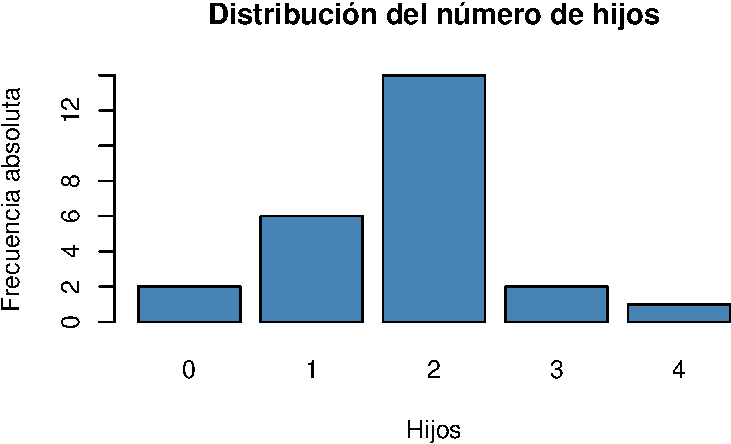
\includegraphics[keepaspectratio]{04-frecuencias-graficos_files/figure-pdf/unnamed-chunk-6-1.pdf}}

\begin{Shaded}
\begin{Highlighting}[]
\CommentTok{\# Diagrama de barras de frecuencias relativas.}
\FunctionTok{barplot}\NormalTok{(fi, }\AttributeTok{col =} \StringTok{"steelblue"}\NormalTok{, }\AttributeTok{main=}\StringTok{"Distribución del número de hijos"}\NormalTok{, }\AttributeTok{xlab=}\StringTok{"Hijos"}\NormalTok{, }\AttributeTok{ylab=}\StringTok{"Frecuencia relativa"}\NormalTok{)}
\end{Highlighting}
\end{Shaded}

  \pandocbounded{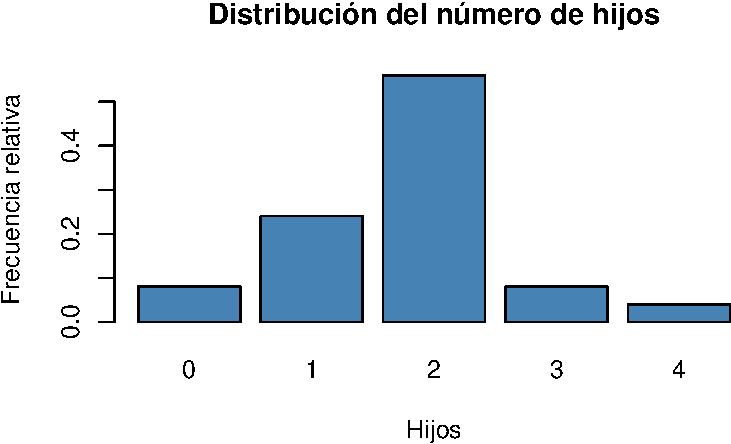
\includegraphics[keepaspectratio]{04-frecuencias-graficos_files/figure-pdf/unnamed-chunk-6-2.pdf}}

\begin{Shaded}
\begin{Highlighting}[]
\CommentTok{\# Diagrama de barras de frecuencias absolutas acumuladas.}
\FunctionTok{barplot}\NormalTok{(Ni, }\AttributeTok{col =} \StringTok{"steelblue"}\NormalTok{, }\AttributeTok{main=}\StringTok{"Distribución acumulada del número de hijos"}\NormalTok{, }\AttributeTok{xlab=}\StringTok{"Hijos"}\NormalTok{, }\AttributeTok{ylab=}\StringTok{"Frecuencia absoluta acumulada"}\NormalTok{)}
\end{Highlighting}
\end{Shaded}

  \pandocbounded{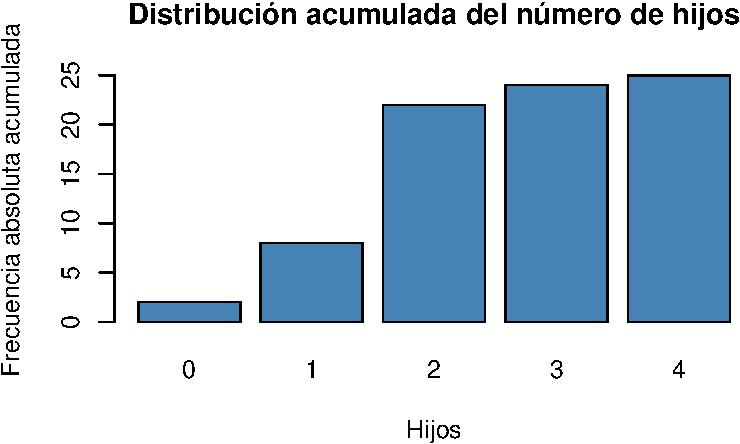
\includegraphics[keepaspectratio]{04-frecuencias-graficos_files/figure-pdf/unnamed-chunk-6-3.pdf}}

\begin{Shaded}
\begin{Highlighting}[]
\CommentTok{\# Diagrama de barras de frecuencias relativas acumuladas.}
\FunctionTok{barplot}\NormalTok{(Fi, }\AttributeTok{col =} \StringTok{"steelblue"}\NormalTok{, }\AttributeTok{main=}\StringTok{"Distribución acumulada del número de hijos"}\NormalTok{, }\AttributeTok{xlab=}\StringTok{"Hijos"}\NormalTok{, }\AttributeTok{ylab=}\StringTok{"Frecuencia relativa acumulada"}\NormalTok{)}
\end{Highlighting}
\end{Shaded}

  \pandocbounded{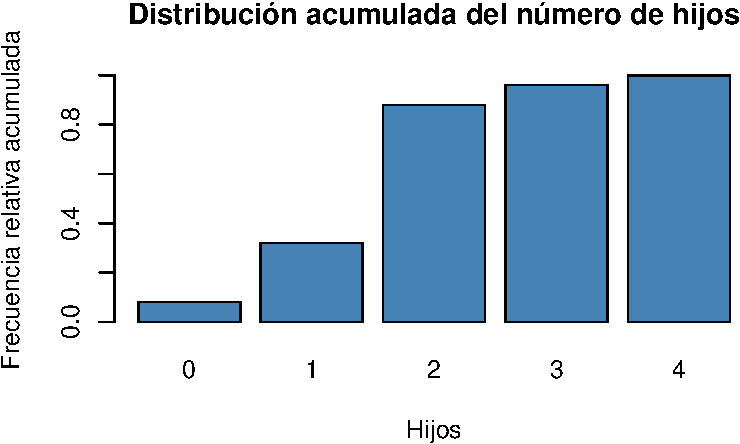
\includegraphics[keepaspectratio]{04-frecuencias-graficos_files/figure-pdf/unnamed-chunk-6-4.pdf}}

  \end{tcolorbox}

  \begin{tcolorbox}[enhanced jigsaw, breakable, toptitle=1mm, colbacktitle=quarto-callout-tip-color!10!white, rightrule=.15mm, opacityback=0, opacitybacktitle=0.6, titlerule=0mm, coltitle=black, colframe=quarto-callout-tip-color-frame, colback=white, bottomtitle=1mm, leftrule=.75mm, toprule=.15mm, title=\textcolor{quarto-callout-tip-color}{\faLightbulb}\hspace{0.5em}{Solución 2}, arc=.35mm, bottomrule=.15mm, left=2mm]

  Otra alternativa es usar la función la función
  \href{https://aprendeconalf.es/manual-r/07-graficos.html\#diagramas-de-barras}{\texttt{geom\_bar}}
  del paquete \texttt{ggplot2}.

\begin{Shaded}
\begin{Highlighting}[]
\FunctionTok{library}\NormalTok{(ggplot2)}
\CommentTok{\# Diagarma de barras de frecuencias absolutas}
\FunctionTok{ggplot}\NormalTok{(df, }\FunctionTok{aes}\NormalTok{(}\AttributeTok{x =}\NormalTok{ hijos)) }\SpecialCharTok{+}
    \FunctionTok{geom\_bar}\NormalTok{(}\AttributeTok{fill =} \StringTok{"steelblue"}\NormalTok{) }\SpecialCharTok{+} 
    \FunctionTok{labs}\NormalTok{(}\AttributeTok{title =} \StringTok{"Distribución del número de hijos"}\NormalTok{, }\AttributeTok{y =} \StringTok{"Frecuencia absoluta"}\NormalTok{)}
\end{Highlighting}
\end{Shaded}

  \pandocbounded{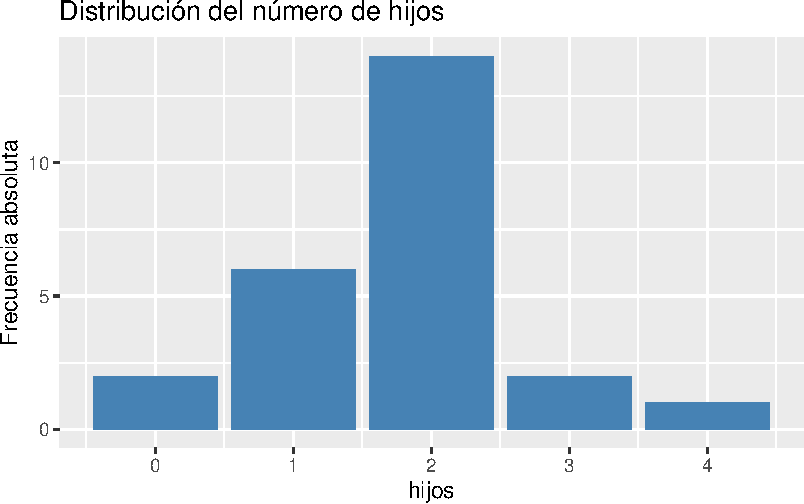
\includegraphics[keepaspectratio]{04-frecuencias-graficos_files/figure-pdf/unnamed-chunk-7-1.pdf}}

\begin{Shaded}
\begin{Highlighting}[]
\CommentTok{\# Diagarma de barras de frecuencias relativas}
\FunctionTok{ggplot}\NormalTok{(df, }\FunctionTok{aes}\NormalTok{(}\AttributeTok{x =}\NormalTok{ hijos)) }\SpecialCharTok{+}
    \FunctionTok{geom\_bar}\NormalTok{(}\FunctionTok{aes}\NormalTok{(}\AttributeTok{y =} \FunctionTok{after\_stat}\NormalTok{(count}\SpecialCharTok{/}\FunctionTok{sum}\NormalTok{(count))), }\AttributeTok{fill =} \StringTok{"steelblue"}\NormalTok{) }\SpecialCharTok{+}
    \FunctionTok{labs}\NormalTok{(}\AttributeTok{title =} \StringTok{"Distribución del número de hijos"}\NormalTok{, }\AttributeTok{y =} \StringTok{"Frecuencia relativa"}\NormalTok{)}
\end{Highlighting}
\end{Shaded}

  \pandocbounded{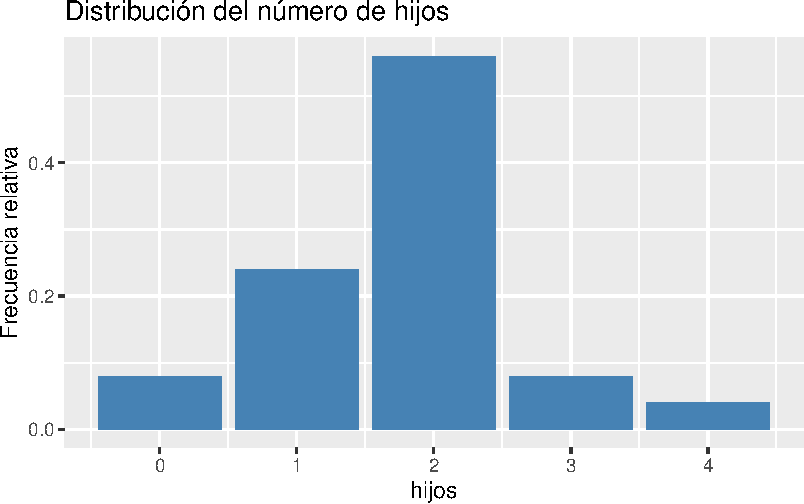
\includegraphics[keepaspectratio]{04-frecuencias-graficos_files/figure-pdf/unnamed-chunk-7-2.pdf}}

\begin{Shaded}
\begin{Highlighting}[]
\CommentTok{\# Diagarma de barras de frecuencias acumuladas}
\FunctionTok{ggplot}\NormalTok{(df, }\FunctionTok{aes}\NormalTok{(}\AttributeTok{x =}\NormalTok{ hijos)) }\SpecialCharTok{+}
    \FunctionTok{geom\_bar}\NormalTok{(}\FunctionTok{aes}\NormalTok{(}\AttributeTok{y =} \FunctionTok{after\_stat}\NormalTok{(}\FunctionTok{cumsum}\NormalTok{(count))), }\AttributeTok{fill =} \StringTok{"steelblue"}\NormalTok{) }\SpecialCharTok{+}
    \FunctionTok{labs}\NormalTok{(}\AttributeTok{title =} \StringTok{"Distribución acumulada del número de hijos"}\NormalTok{, }\AttributeTok{y =} \StringTok{"Frecuencia absoluta acumulada"}\NormalTok{)}
\end{Highlighting}
\end{Shaded}

  \pandocbounded{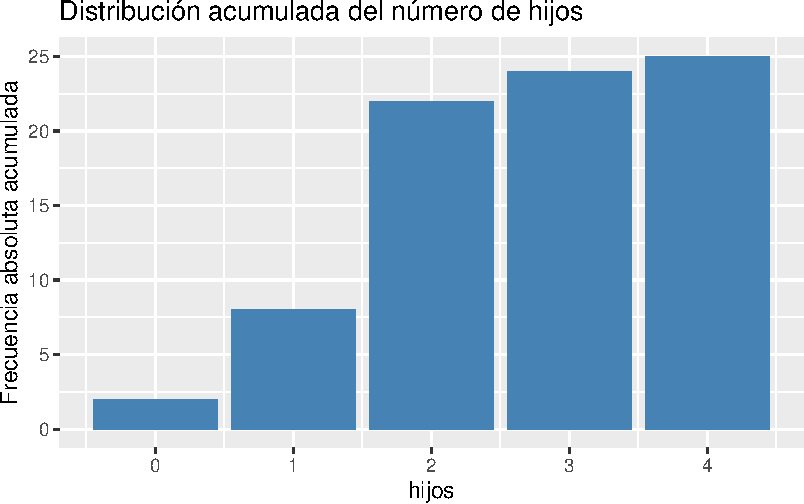
\includegraphics[keepaspectratio]{04-frecuencias-graficos_files/figure-pdf/unnamed-chunk-7-3.pdf}}

\begin{Shaded}
\begin{Highlighting}[]
\CommentTok{\# Diagarma de barras de frecuencias acumuladas}
\FunctionTok{ggplot}\NormalTok{(df, }\FunctionTok{aes}\NormalTok{(}\AttributeTok{x =}\NormalTok{ hijos)) }\SpecialCharTok{+}
    \FunctionTok{geom\_bar}\NormalTok{(}\FunctionTok{aes}\NormalTok{(}\AttributeTok{y =} \FunctionTok{after\_stat}\NormalTok{(}\FunctionTok{cumsum}\NormalTok{(count)}\SpecialCharTok{/}\FunctionTok{sum}\NormalTok{(count))), }\AttributeTok{fill =} \StringTok{"steelblue"}\NormalTok{) }\SpecialCharTok{+}
    \FunctionTok{labs}\NormalTok{(}\AttributeTok{title =} \StringTok{"Distribución acumulada del número de hijos"}\NormalTok{, }\AttributeTok{y =} \StringTok{"Frecuencia relativa acumulada"}\NormalTok{)}
\end{Highlighting}
\end{Shaded}

  \pandocbounded{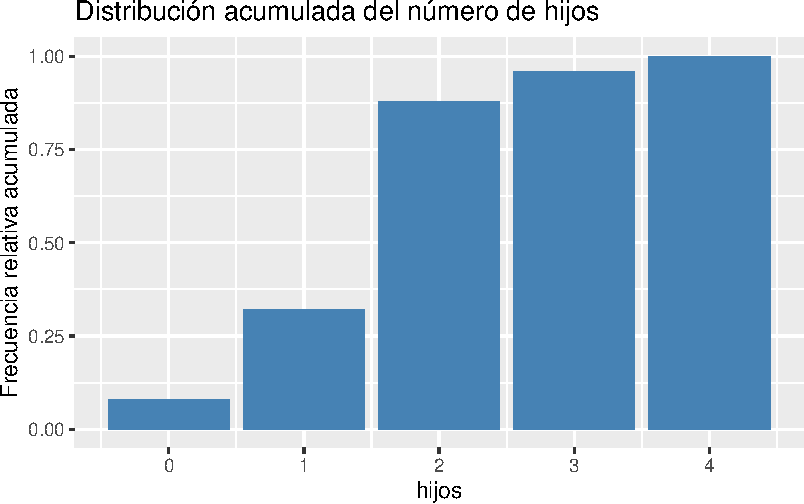
\includegraphics[keepaspectratio]{04-frecuencias-graficos_files/figure-pdf/unnamed-chunk-7-4.pdf}}

  \end{tcolorbox}
\item
  Dibujar el polígono de frecuencias relativas.

  \begin{tcolorbox}[enhanced jigsaw, breakable, toptitle=1mm, colbacktitle=quarto-callout-tip-color!10!white, rightrule=.15mm, opacityback=0, opacitybacktitle=0.6, titlerule=0mm, coltitle=black, colframe=quarto-callout-tip-color-frame, colback=white, bottomtitle=1mm, leftrule=.75mm, toprule=.15mm, title=\textcolor{quarto-callout-tip-color}{\faLightbulb}\hspace{0.5em}{Solución 1}, arc=.35mm, bottomrule=.15mm, left=2mm]

  Para dibujar un diagrama de lineas se puede usar la función
  \href{https://www.rdocumentation.org/packages/graphics/versions/3.6.2/topics/plot}{\texttt{plot}}
  del paquete \texttt{graphics}.

\begin{Shaded}
\begin{Highlighting}[]
\CommentTok{\# Frecuencias relativas.}
\FunctionTok{plot}\NormalTok{(}\FunctionTok{names}\NormalTok{(fi), fi, }\AttributeTok{type =} \StringTok{"l"}\NormalTok{, }\AttributeTok{col =} \StringTok{"steelblue"}\NormalTok{, }\AttributeTok{main=}\StringTok{"Distribución del número de hijos"}\NormalTok{, }\AttributeTok{xlab=}\StringTok{"Hijos"}\NormalTok{, }\AttributeTok{ylab=}\StringTok{"Frecuencia relativa"}\NormalTok{)}
\end{Highlighting}
\end{Shaded}

  \pandocbounded{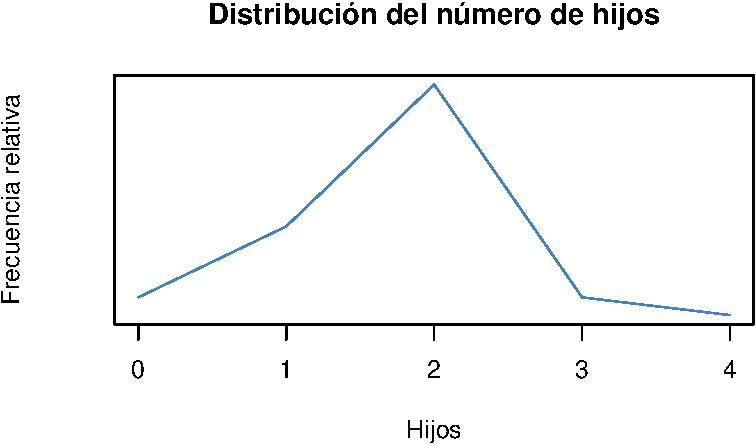
\includegraphics[keepaspectratio]{04-frecuencias-graficos_files/figure-pdf/unnamed-chunk-8-1.pdf}}

  \end{tcolorbox}

  \begin{tcolorbox}[enhanced jigsaw, breakable, toptitle=1mm, colbacktitle=quarto-callout-tip-color!10!white, rightrule=.15mm, opacityback=0, opacitybacktitle=0.6, titlerule=0mm, coltitle=black, colframe=quarto-callout-tip-color-frame, colback=white, bottomtitle=1mm, leftrule=.75mm, toprule=.15mm, title=\textcolor{quarto-callout-tip-color}{\faLightbulb}\hspace{0.5em}{Solución 2}, arc=.35mm, bottomrule=.15mm, left=2mm]

  Otra alternativa es usar la función la función
  \href{https://aprendeconalf.es/manual-r/07-graficos.html\#diagramas-de-lineas}{\texttt{geom\_line}}
  del paquete \texttt{ggplot2}.

\begin{Shaded}
\begin{Highlighting}[]
\FunctionTok{library}\NormalTok{(ggplot2)}
\FunctionTok{count}\NormalTok{(df, hijos) }\SpecialCharTok{|\textgreater{}} 
    \FunctionTok{mutate}\NormalTok{(}\AttributeTok{fi =}\NormalTok{ n}\SpecialCharTok{/}\FunctionTok{sum}\NormalTok{(n)) }\SpecialCharTok{|\textgreater{}}
    \FunctionTok{ggplot}\NormalTok{(}\FunctionTok{aes}\NormalTok{(}\AttributeTok{x=}\NormalTok{hijos, }\AttributeTok{y=}\NormalTok{fi)) }\SpecialCharTok{+}
    \FunctionTok{geom\_line}\NormalTok{(}\AttributeTok{col =} \StringTok{"steelblue"}\NormalTok{) }\SpecialCharTok{+}
    \FunctionTok{labs}\NormalTok{(}\AttributeTok{title =} \StringTok{"Distribución del número de hijos"}\NormalTok{, }\AttributeTok{y =} \StringTok{"Frecuencia relativa"}\NormalTok{)}
\end{Highlighting}
\end{Shaded}

  \pandocbounded{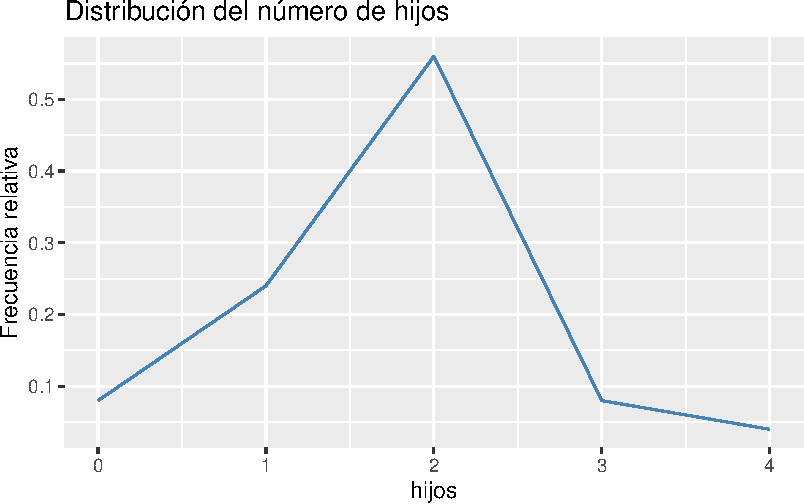
\includegraphics[keepaspectratio]{04-frecuencias-graficos_files/figure-pdf/unnamed-chunk-9-1.pdf}}

  \end{tcolorbox}
\end{enumerate}

\end{exercise}

\begin{exercise}[]\protect\hypertarget{exr-frecuencias-graficos-2}{}\label{exr-frecuencias-graficos-2}

En un servicio de atención al cliente se han registrado el número de
llamadas de clientes cada día del mes de noviembre, obteniendo los
siguientes datos:

\begin{longtable}[]{@{}
  >{\centering\arraybackslash}p{(\linewidth - 0\tabcolsep) * \real{1.0000}}@{}}
\toprule\noalign{}
\endhead
\bottomrule\noalign{}
\endlastfoot
15, 23, 12, 10, 28, 50, 12, 17, 20, 21, 18, 13, 11, 12, 26, 30, 6, 16,
19, 22, 14, 17, 21, 28, 9, 16, 13, 11, 16, 20 \\
\end{longtable}

\begin{enumerate}
\def\labelenumi{\alph{enumi}.}
\item
  Crear un conjunto de datos con la variable \texttt{llamadas}.

  \begin{tcolorbox}[enhanced jigsaw, breakable, toptitle=1mm, colbacktitle=quarto-callout-tip-color!10!white, rightrule=.15mm, opacityback=0, opacitybacktitle=0.6, titlerule=0mm, coltitle=black, colframe=quarto-callout-tip-color-frame, colback=white, bottomtitle=1mm, leftrule=.75mm, toprule=.15mm, title=\textcolor{quarto-callout-tip-color}{\faLightbulb}\hspace{0.5em}{Solución}, arc=.35mm, bottomrule=.15mm, left=2mm]

\begin{Shaded}
\begin{Highlighting}[]
\NormalTok{df }\OtherTok{\textless{}{-}} \FunctionTok{data.frame}\NormalTok{(}\AttributeTok{llamadas =} \FunctionTok{c}\NormalTok{(}\DecValTok{15}\NormalTok{, }\DecValTok{23}\NormalTok{, }\DecValTok{12}\NormalTok{, }\DecValTok{10}\NormalTok{, }\DecValTok{28}\NormalTok{, }\DecValTok{50}\NormalTok{, }\DecValTok{12}\NormalTok{, }\DecValTok{17}\NormalTok{, }\DecValTok{20}\NormalTok{, }\DecValTok{21}\NormalTok{, }\DecValTok{18}\NormalTok{, }\DecValTok{13}\NormalTok{, }\DecValTok{11}\NormalTok{, }\DecValTok{12}\NormalTok{, }\DecValTok{26}\NormalTok{, }\DecValTok{30}\NormalTok{, }\DecValTok{6}\NormalTok{, }\DecValTok{16}\NormalTok{, }\DecValTok{19}\NormalTok{, }\DecValTok{22}\NormalTok{, }\DecValTok{14}\NormalTok{, }\DecValTok{17}\NormalTok{, }\DecValTok{21}\NormalTok{, }\DecValTok{28}\NormalTok{, }\DecValTok{9}\NormalTok{, }\DecValTok{16}\NormalTok{, }\DecValTok{13}\NormalTok{, }\DecValTok{11}\NormalTok{, }\DecValTok{16}\NormalTok{, }\DecValTok{20}\NormalTok{))}
\end{Highlighting}
\end{Shaded}

  \end{tcolorbox}
\item
  Dibujar el diagrama de cajas. ¿Existe algún dato atípico? En el caso
  de que exista, eliminarlo y proceder con los siguientes apartados.

  \begin{tcolorbox}[enhanced jigsaw, breakable, toptitle=1mm, colbacktitle=quarto-callout-tip-color!10!white, rightrule=.15mm, opacityback=0, opacitybacktitle=0.6, titlerule=0mm, coltitle=black, colframe=quarto-callout-tip-color-frame, colback=white, bottomtitle=1mm, leftrule=.75mm, toprule=.15mm, title=\textcolor{quarto-callout-tip-color}{\faLightbulb}\hspace{0.5em}{Solución 1}, arc=.35mm, bottomrule=.15mm, left=2mm]

  Para dibujar un diagrama de cajas se puede usar la función
  \href{https://www.rdocumentation.org/packages/graphics/versions/3.6.2/topics/boxplot}{\texttt{boxplot}}
  del paquete \texttt{graphics}.

\begin{Shaded}
\begin{Highlighting}[]
\CommentTok{\# Frecuencias relativas.}
\FunctionTok{boxplot}\NormalTok{(df}\SpecialCharTok{$}\NormalTok{llamadas, }\AttributeTok{col =} \StringTok{"steelblue"}\NormalTok{, }\AttributeTok{main=}\StringTok{"Distribución del número de llamadas"}\NormalTok{, }\AttributeTok{horizontal =}\NormalTok{ T, }\AttributeTok{xlab=}\StringTok{"Número de llamadas"}\NormalTok{)}
\end{Highlighting}
\end{Shaded}

  \pandocbounded{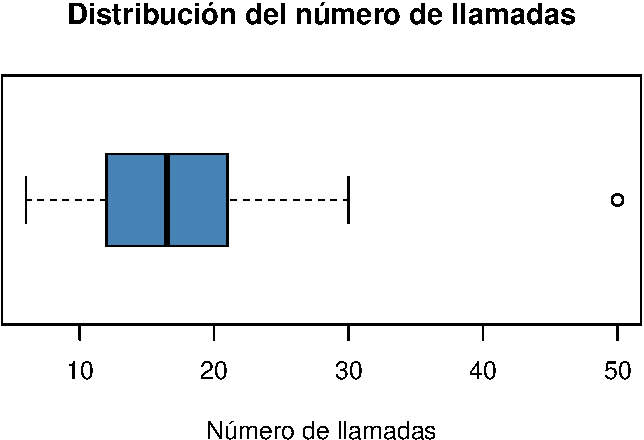
\includegraphics[keepaspectratio]{04-frecuencias-graficos_files/figure-pdf/unnamed-chunk-11-1.pdf}}

  \end{tcolorbox}

  \begin{tcolorbox}[enhanced jigsaw, breakable, toptitle=1mm, colbacktitle=quarto-callout-tip-color!10!white, rightrule=.15mm, opacityback=0, opacitybacktitle=0.6, titlerule=0mm, coltitle=black, colframe=quarto-callout-tip-color-frame, colback=white, bottomtitle=1mm, leftrule=.75mm, toprule=.15mm, title=\textcolor{quarto-callout-tip-color}{\faLightbulb}\hspace{0.5em}{Solución 2}, arc=.35mm, bottomrule=.15mm, left=2mm]

  Otra alternativa es usar la función la función
  \href{https://aprendeconalf.es/manual-r/07-graficos.html\#diagramas-de-cajas}{\texttt{geom\_boxplot}}
  del paquete \texttt{ggplot2}.

\begin{Shaded}
\begin{Highlighting}[]
\FunctionTok{library}\NormalTok{(ggplot2)}
\FunctionTok{ggplot}\NormalTok{(df, }\FunctionTok{aes}\NormalTok{(}\AttributeTok{x =}\NormalTok{ llamadas)) }\SpecialCharTok{+}
    \FunctionTok{geom\_boxplot}\NormalTok{(}\AttributeTok{fill =} \StringTok{"steelblue"}\NormalTok{) }\SpecialCharTok{+}
    \FunctionTok{labs}\NormalTok{(}\AttributeTok{title =} \StringTok{"Distribución del número de llamadas"}\NormalTok{, }\AttributeTok{x =} \StringTok{"Número de llamadas"}\NormalTok{)}
\end{Highlighting}
\end{Shaded}

  \pandocbounded{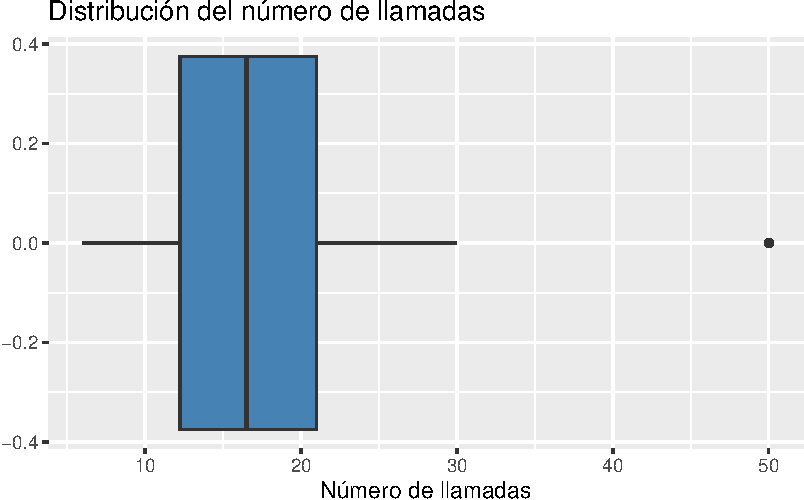
\includegraphics[keepaspectratio]{04-frecuencias-graficos_files/figure-pdf/unnamed-chunk-12-1.pdf}}

  Hay un día con 50 llamadas, que es un valor atípico en comparación con
  el resto de días.

  \begin{tcolorbox}[enhanced jigsaw, breakable, toptitle=1mm, colbacktitle=quarto-callout-tip-color!10!white, rightrule=.15mm, opacityback=0, opacitybacktitle=0.6, titlerule=0mm, coltitle=black, colframe=quarto-callout-tip-color-frame, colback=white, bottomtitle=1mm, leftrule=.75mm, toprule=.15mm, title=\textcolor{quarto-callout-tip-color}{\faLightbulb}\hspace{0.5em}{Solución}, arc=.35mm, bottomrule=.15mm, left=2mm]

  La función \texttt{cut}

\begin{Shaded}
\begin{Highlighting}[]
\CommentTok{\# Eliminación del dato atípico.}
\NormalTok{df }\OtherTok{\textless{}{-}}\NormalTok{ df[df}\SpecialCharTok{$}\NormalTok{llamadas }\SpecialCharTok{!=} \DecValTok{50}\NormalTok{, , drop }\OtherTok{=}\NormalTok{ F]}
\end{Highlighting}
\end{Shaded}

  \end{tcolorbox}

  \end{tcolorbox}
\item
  Construir la tabla de frecuencias agrupando en 5 clases.

  \begin{tcolorbox}[enhanced jigsaw, breakable, toptitle=1mm, colbacktitle=quarto-callout-tip-color!10!white, rightrule=.15mm, opacityback=0, opacitybacktitle=0.6, titlerule=0mm, coltitle=black, colframe=quarto-callout-tip-color-frame, colback=white, bottomtitle=1mm, leftrule=.75mm, toprule=.15mm, title=\textcolor{quarto-callout-tip-color}{\faLightbulb}\hspace{0.5em}{Solución 1}, arc=.35mm, bottomrule=.15mm, left=2mm]

  Para agrupar los datos en intervalos se puede utilizar la función
  \href{https://www.rdocumentation.org/packages/base/versions/3.6.2/topics/cut}{\texttt{cut}}
  del paquete base de R, y para contar las frecuencias absolutas y
  relativas las funciones
  \href{https://www.rdocumentation.org/packages/base/versions/3.6.2/topics/table}{\texttt{table}},
  y
  \href{https://www.rdocumentation.org/packages/base/versions/3.6.2/topics/prop.table}{\texttt{prop.table}}
  respectivamente.

\begin{Shaded}
\begin{Highlighting}[]
\CommentTok{\# Frecuencias absolutas. Creación automática de 5 clases con intervalos cerrados a la izquierda.}
\end{Highlighting}
\end{Shaded}

\begin{Shaded}
\begin{Highlighting}[]
\NormalTok{ni }\OtherTok{\textless{}{-}} \FunctionTok{table}\NormalTok{(}\FunctionTok{cut}\NormalTok{(df}\SpecialCharTok{$}\NormalTok{llamadas, }\AttributeTok{breaks =} \DecValTok{5}\NormalTok{, }\AttributeTok{right =}\NormalTok{ F))}
\CommentTok{\# Creación manual de 5 clases.}
\NormalTok{ni }\OtherTok{\textless{}{-}} \FunctionTok{table}\NormalTok{(}\FunctionTok{cut}\NormalTok{(df}\SpecialCharTok{$}\NormalTok{llamadas, }\AttributeTok{breaks =} \FunctionTok{seq}\NormalTok{(}\DecValTok{5}\NormalTok{, }\DecValTok{30}\NormalTok{, }\DecValTok{5}\NormalTok{)))}
\CommentTok{\# Frecuencias relativas}
\NormalTok{fi }\OtherTok{\textless{}{-}} \FunctionTok{prop.table}\NormalTok{(ni)}
\CommentTok{\# Frecuencias acumuladas.}
\NormalTok{Ni }\OtherTok{\textless{}{-}} \FunctionTok{cumsum}\NormalTok{(ni)}
\CommentTok{\# Frecuencias relativas acumuladas.}
\NormalTok{Fi }\OtherTok{\textless{}{-}} \FunctionTok{cumsum}\NormalTok{(fi)}
\CommentTok{\# Creación de un data frame con las frecuencias.}
\NormalTok{tabla\_frec }\OtherTok{\textless{}{-}} \FunctionTok{cbind}\NormalTok{(ni, fi, Ni, Fi)}
\NormalTok{tabla\_frec}
\end{Highlighting}
\end{Shaded}

\begin{verbatim}
        ni        fi Ni        Fi
(5,10]   3 0.1034483  3 0.1034483
(10,15]  9 0.3103448 12 0.4137931
(15,20]  9 0.3103448 21 0.7241379
(20,25]  4 0.1379310 25 0.8620690
(25,30]  4 0.1379310 29 1.0000000
\end{verbatim}

  \end{tcolorbox}

  \begin{tcolorbox}[enhanced jigsaw, breakable, toptitle=1mm, colbacktitle=quarto-callout-tip-color!10!white, rightrule=.15mm, opacityback=0, opacitybacktitle=0.6, titlerule=0mm, coltitle=black, colframe=quarto-callout-tip-color-frame, colback=white, bottomtitle=1mm, leftrule=.75mm, toprule=.15mm, title=\textcolor{quarto-callout-tip-color}{\faLightbulb}\hspace{0.5em}{Solución 2}, arc=.35mm, bottomrule=.15mm, left=2mm]

  Otra alternativa es usar la fución
  \href{https://aprendeconalf.es/manual-r/06-preprocesamiento.html\#conteo-del-n\%C3\%BAmero-de-observaciones}{\texttt{count}}
  del paquete \texttt{dplyr}.

\begin{Shaded}
\begin{Highlighting}[]
\FunctionTok{library}\NormalTok{(dplyr)}
\FunctionTok{library}\NormalTok{(knitr)}
\FunctionTok{library}\NormalTok{(kableExtra)}
\FunctionTok{mutate}\NormalTok{(df, }\AttributeTok{llamadas\_int =} \FunctionTok{cut}\NormalTok{(llamadas, }\AttributeTok{breaks =} \FunctionTok{seq}\NormalTok{(}\DecValTok{5}\NormalTok{, }\DecValTok{30}\NormalTok{, }\DecValTok{5}\NormalTok{))) }\SpecialCharTok{|\textgreater{}} 
    \FunctionTok{count}\NormalTok{(llamadas\_int) }\SpecialCharTok{|\textgreater{}}
    \FunctionTok{mutate}\NormalTok{(}\AttributeTok{fi =}\NormalTok{ n}\SpecialCharTok{/}\FunctionTok{sum}\NormalTok{(n), }\AttributeTok{Ni =} \FunctionTok{cumsum}\NormalTok{(n), }\AttributeTok{Fi =} \FunctionTok{cumsum}\NormalTok{(n)}\SpecialCharTok{/}\FunctionTok{sum}\NormalTok{(n)) }\SpecialCharTok{|\textgreater{}}
    \FunctionTok{kable}\NormalTok{()}
\end{Highlighting}
\end{Shaded}

  \begin{longtable}[]{@{}lrrrr@{}}
  \toprule\noalign{}
  llamadas\_int & n & fi & Ni & Fi \\
  \midrule\noalign{}
  \endhead
  \bottomrule\noalign{}
  \endlastfoot
  (5,10{]} & 3 & 0.1034483 & 3 & 0.1034483 \\
  (10,15{]} & 9 & 0.3103448 & 12 & 0.4137931 \\
  (15,20{]} & 9 & 0.3103448 & 21 & 0.7241379 \\
  (20,25{]} & 4 & 0.1379310 & 25 & 0.8620690 \\
  (25,30{]} & 4 & 0.1379310 & 29 & 1.0000000 \\
  \end{longtable}

  \end{tcolorbox}
\item
  Dibujar el histograma de frecuencias absolutas, relativas, absolutas
  acumuladas y relativas acumuladas correspondiente a la tabla anterior.

  \begin{tcolorbox}[enhanced jigsaw, breakable, toptitle=1mm, colbacktitle=quarto-callout-tip-color!10!white, rightrule=.15mm, opacityback=0, opacitybacktitle=0.6, titlerule=0mm, coltitle=black, colframe=quarto-callout-tip-color-frame, colback=white, bottomtitle=1mm, leftrule=.75mm, toprule=.15mm, title=\textcolor{quarto-callout-tip-color}{\faLightbulb}\hspace{0.5em}{Solución 1}, arc=.35mm, bottomrule=.15mm, left=2mm]

  Para dibujar un histograma se puede usar la función
  \href{https://www.rdocumentation.org/packages/graphics/versions/3.6.2/topics/hist}{\texttt{hist}}
  del paquete \texttt{graphics}.

\begin{Shaded}
\begin{Highlighting}[]
\CommentTok{\# Histograma de frecuencias absolutas.}
\NormalTok{histo }\OtherTok{\textless{}{-}} \FunctionTok{hist}\NormalTok{(df}\SpecialCharTok{$}\NormalTok{llamadas, }\AttributeTok{breaks =} \FunctionTok{seq}\NormalTok{(}\DecValTok{5}\NormalTok{, }\DecValTok{30}\NormalTok{, }\DecValTok{5}\NormalTok{), }\AttributeTok{col =} \StringTok{"steelblue"}\NormalTok{, }\AttributeTok{main=}\StringTok{"Distribución del número de llamadas"}\NormalTok{, }\AttributeTok{xlab=}\StringTok{"Llamadas"}\NormalTok{, }\AttributeTok{ylab=}\StringTok{"Frecuencia absoluta"}\NormalTok{)}
\end{Highlighting}
\end{Shaded}

  \pandocbounded{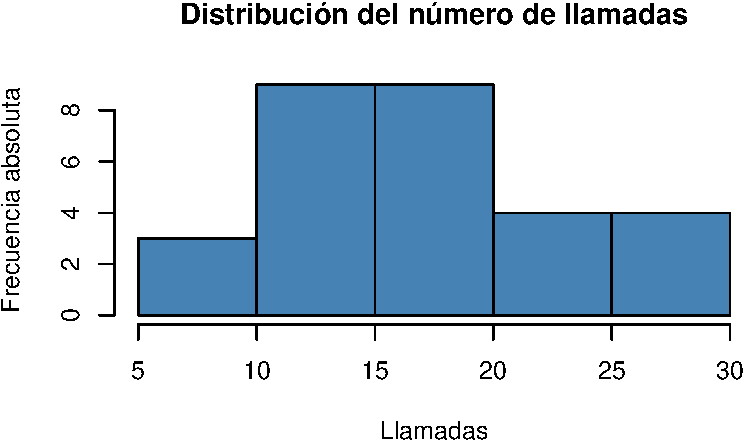
\includegraphics[keepaspectratio]{04-frecuencias-graficos_files/figure-pdf/unnamed-chunk-18-1.pdf}}

\begin{Shaded}
\begin{Highlighting}[]
\NormalTok{ni }\OtherTok{\textless{}{-}}\NormalTok{ histo}\SpecialCharTok{$}\NormalTok{counts}
\CommentTok{\# Histograma de frecuencias relativas.}
\NormalTok{histo}\SpecialCharTok{$}\NormalTok{counts }\OtherTok{\textless{}{-}}\NormalTok{ ni}\SpecialCharTok{/}\FunctionTok{sum}\NormalTok{(ni)}
\FunctionTok{plot}\NormalTok{(histo, }\AttributeTok{col =} \StringTok{"steelblue"}\NormalTok{, }\AttributeTok{main=}\StringTok{"Distribución del número de llamadas"}\NormalTok{, }\AttributeTok{xlab=}\StringTok{"Llamadas"}\NormalTok{, }\AttributeTok{ylab=}\StringTok{"Frecuencia relativa"}\NormalTok{)}
\end{Highlighting}
\end{Shaded}

  \pandocbounded{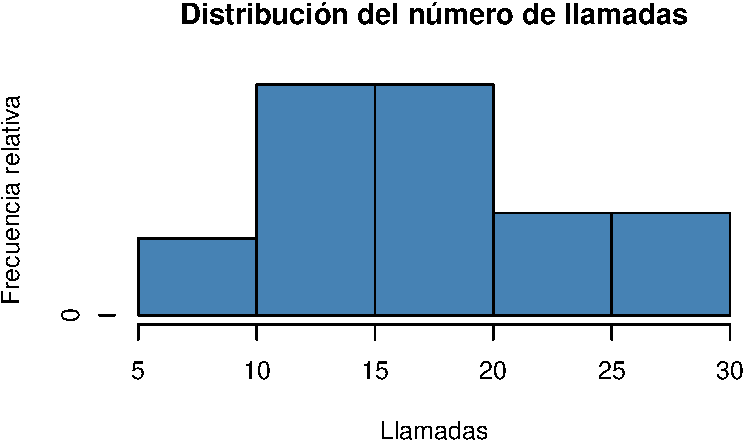
\includegraphics[keepaspectratio]{04-frecuencias-graficos_files/figure-pdf/unnamed-chunk-18-2.pdf}}

\begin{Shaded}
\begin{Highlighting}[]
\CommentTok{\# Histograma de frecuencias absolutas acumuladas.}
\NormalTok{histo}\SpecialCharTok{$}\NormalTok{counts }\OtherTok{\textless{}{-}} \FunctionTok{cumsum}\NormalTok{(ni)}
\FunctionTok{plot}\NormalTok{(histo, }\AttributeTok{col =} \StringTok{"steelblue"}\NormalTok{, }\AttributeTok{main=}\StringTok{"Distribución acumulada del número de llamadas"}\NormalTok{, }\AttributeTok{xlab=}\StringTok{"Llamadas"}\NormalTok{, }\AttributeTok{ylab=}\StringTok{"Frecuencia absoluta acumulada"}\NormalTok{)}
\end{Highlighting}
\end{Shaded}

  \pandocbounded{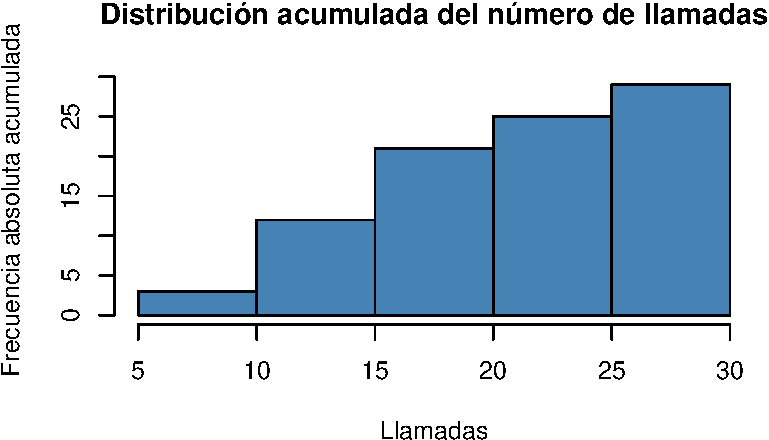
\includegraphics[keepaspectratio]{04-frecuencias-graficos_files/figure-pdf/unnamed-chunk-18-3.pdf}}

\begin{Shaded}
\begin{Highlighting}[]
\CommentTok{\# Histograma de frecuencias relativas acumuladas.}
\NormalTok{histo}\SpecialCharTok{$}\NormalTok{counts }\OtherTok{\textless{}{-}} \FunctionTok{cumsum}\NormalTok{(ni)}\SpecialCharTok{/}\FunctionTok{sum}\NormalTok{(ni)}
\FunctionTok{plot}\NormalTok{(histo, }\AttributeTok{col =} \StringTok{"steelblue"}\NormalTok{, }\AttributeTok{main=}\StringTok{"Distribución acumulada del número de llamadas"}\NormalTok{, }\AttributeTok{xlab=}\StringTok{"Llamadas"}\NormalTok{, }\AttributeTok{ylab=}\StringTok{"Frecuencia relativa acumulada"}\NormalTok{, )}
\end{Highlighting}
\end{Shaded}

  \pandocbounded{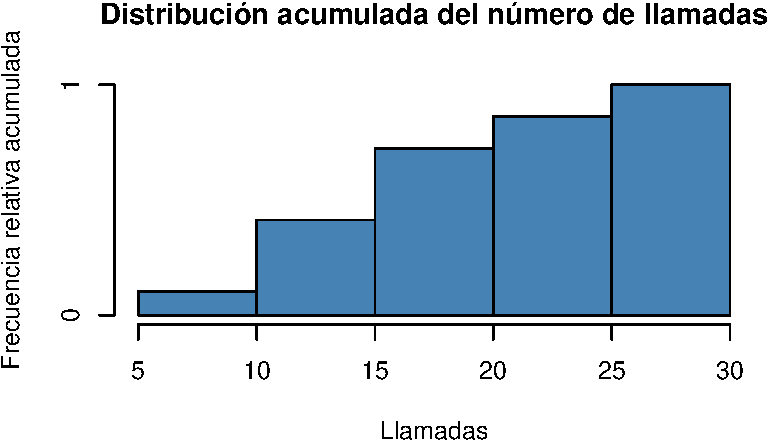
\includegraphics[keepaspectratio]{04-frecuencias-graficos_files/figure-pdf/unnamed-chunk-18-4.pdf}}

  \end{tcolorbox}

  \begin{tcolorbox}[enhanced jigsaw, breakable, toptitle=1mm, colbacktitle=quarto-callout-tip-color!10!white, rightrule=.15mm, opacityback=0, opacitybacktitle=0.6, titlerule=0mm, coltitle=black, colframe=quarto-callout-tip-color-frame, colback=white, bottomtitle=1mm, leftrule=.75mm, toprule=.15mm, title=\textcolor{quarto-callout-tip-color}{\faLightbulb}\hspace{0.5em}{Solución 2}, arc=.35mm, bottomrule=.15mm, left=2mm]

  Otra alternativa es usar la función la función
  \href{https://aprendeconalf.es/manual-r/07-graficos.html\#histogramas}{\texttt{geom\_histogram}}
  del paquete \texttt{ggplot2}.

\begin{Shaded}
\begin{Highlighting}[]
\FunctionTok{library}\NormalTok{(ggplot2)}
\CommentTok{\# Histograma de frecuencias absolutas}
\FunctionTok{ggplot}\NormalTok{(df, }\FunctionTok{aes}\NormalTok{(}\AttributeTok{x =}\NormalTok{ llamadas)) }\SpecialCharTok{+}
    \FunctionTok{geom\_histogram}\NormalTok{(}\AttributeTok{breaks =} \FunctionTok{seq}\NormalTok{(}\DecValTok{5}\NormalTok{, }\DecValTok{30}\NormalTok{, }\DecValTok{5}\NormalTok{), }\AttributeTok{fill =} \StringTok{"steelblue"}\NormalTok{, }\AttributeTok{col =} \StringTok{"white"}\NormalTok{) }\SpecialCharTok{+} 
    \FunctionTok{labs}\NormalTok{(}\AttributeTok{title =} \StringTok{"Distribución del número de llamadas"}\NormalTok{, }\AttributeTok{x =} \StringTok{"Número de llamadas"}\NormalTok{, }\AttributeTok{y =} \StringTok{"Frecuencia absoluta"}\NormalTok{)}
\end{Highlighting}
\end{Shaded}

  \pandocbounded{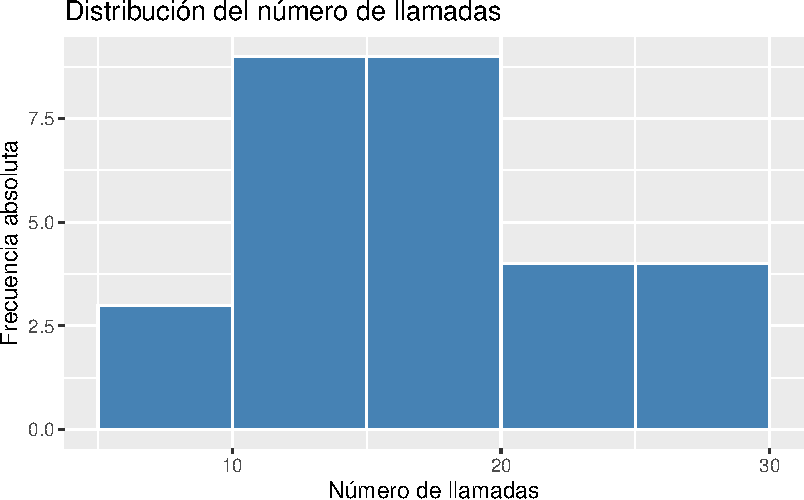
\includegraphics[keepaspectratio]{04-frecuencias-graficos_files/figure-pdf/unnamed-chunk-19-1.pdf}}

\begin{Shaded}
\begin{Highlighting}[]
\CommentTok{\# Histograma de frecuencias relativas}
\FunctionTok{ggplot}\NormalTok{(df, }\FunctionTok{aes}\NormalTok{(}\AttributeTok{x =}\NormalTok{ llamadas)) }\SpecialCharTok{+}
    \FunctionTok{geom\_histogram}\NormalTok{(}\FunctionTok{aes}\NormalTok{(}\AttributeTok{y =} \FunctionTok{after\_stat}\NormalTok{(count}\SpecialCharTok{/}\FunctionTok{sum}\NormalTok{(count))), }\AttributeTok{breaks =} \FunctionTok{seq}\NormalTok{(}\DecValTok{5}\NormalTok{, }\DecValTok{30}\NormalTok{, }\DecValTok{5}\NormalTok{), }\AttributeTok{fill =} \StringTok{"steelblue"}\NormalTok{, }\AttributeTok{col =} \StringTok{"white"}\NormalTok{) }\SpecialCharTok{+}
    \FunctionTok{labs}\NormalTok{(}\AttributeTok{title =} \StringTok{"Distribución del número de llamadas"}\NormalTok{, }\AttributeTok{x =} \StringTok{"Número de llamadas"}\NormalTok{, }\AttributeTok{y =} \StringTok{"Frecuencia relativa"}\NormalTok{)}
\end{Highlighting}
\end{Shaded}

  \pandocbounded{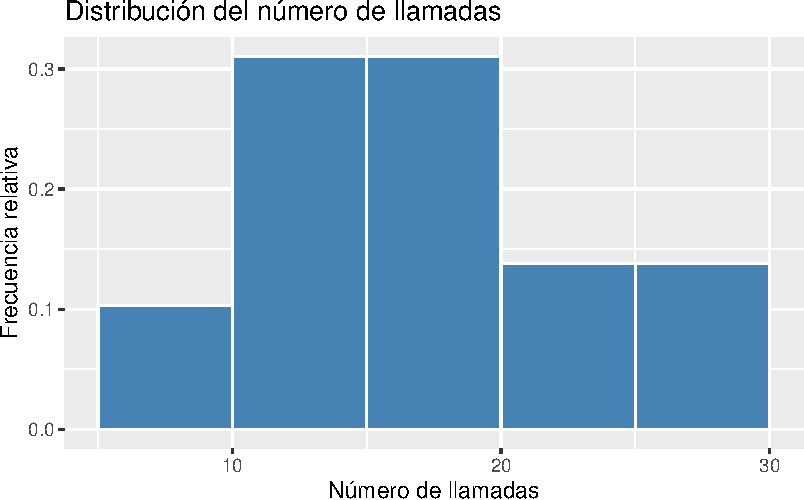
\includegraphics[keepaspectratio]{04-frecuencias-graficos_files/figure-pdf/unnamed-chunk-19-2.pdf}}

\begin{Shaded}
\begin{Highlighting}[]
\CommentTok{\# Histograma de frecuencias acumuladas}
\FunctionTok{ggplot}\NormalTok{(df, }\FunctionTok{aes}\NormalTok{(}\AttributeTok{x =}\NormalTok{ llamadas)) }\SpecialCharTok{+}
    \FunctionTok{geom\_histogram}\NormalTok{(}\FunctionTok{aes}\NormalTok{(}\AttributeTok{y =} \FunctionTok{after\_stat}\NormalTok{(}\FunctionTok{cumsum}\NormalTok{(count))), }\AttributeTok{breaks =} \FunctionTok{seq}\NormalTok{(}\DecValTok{5}\NormalTok{, }\DecValTok{30}\NormalTok{, }\DecValTok{5}\NormalTok{), }\AttributeTok{fill =} \StringTok{"steelblue"}\NormalTok{, }\AttributeTok{col =} \StringTok{"white"}\NormalTok{) }\SpecialCharTok{+}
    \FunctionTok{labs}\NormalTok{(}\AttributeTok{title =} \StringTok{"Distribución acumulada del número de llamadas"}\NormalTok{, }\AttributeTok{x =} \StringTok{"Número de llamadas"}\NormalTok{, }\AttributeTok{y =} \StringTok{"Frecuencia absoluta acumulada"}\NormalTok{)}
\end{Highlighting}
\end{Shaded}

  \pandocbounded{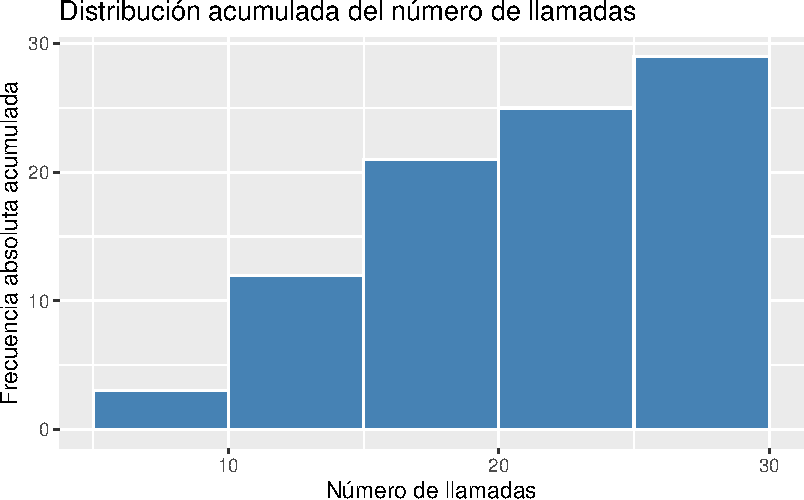
\includegraphics[keepaspectratio]{04-frecuencias-graficos_files/figure-pdf/unnamed-chunk-19-3.pdf}}

\begin{Shaded}
\begin{Highlighting}[]
\CommentTok{\# Histograma de frecuencias relativas acumuladas}
\FunctionTok{ggplot}\NormalTok{(df, }\FunctionTok{aes}\NormalTok{(}\AttributeTok{x =}\NormalTok{ llamadas)) }\SpecialCharTok{+}
    \FunctionTok{geom\_histogram}\NormalTok{(}\FunctionTok{aes}\NormalTok{(}\AttributeTok{y =} \FunctionTok{after\_stat}\NormalTok{(}\FunctionTok{cumsum}\NormalTok{(count)}\SpecialCharTok{/}\FunctionTok{sum}\NormalTok{(count))),  }\AttributeTok{breaks =} \FunctionTok{seq}\NormalTok{(}\DecValTok{5}\NormalTok{, }\DecValTok{30}\NormalTok{, }\DecValTok{5}\NormalTok{), }\AttributeTok{fill =} \StringTok{"steelblue"}\NormalTok{, }\AttributeTok{col =} \StringTok{"white"}\NormalTok{) }\SpecialCharTok{+}
    \FunctionTok{labs}\NormalTok{(}\AttributeTok{title =} \StringTok{"Distribución acumulada del número de llamadas"}\NormalTok{, }\AttributeTok{x =} \StringTok{"Número de llamadas"}\NormalTok{, }\AttributeTok{y =} \StringTok{"Frecuencia relativa acumulada"}\NormalTok{)}
\end{Highlighting}
\end{Shaded}

  \pandocbounded{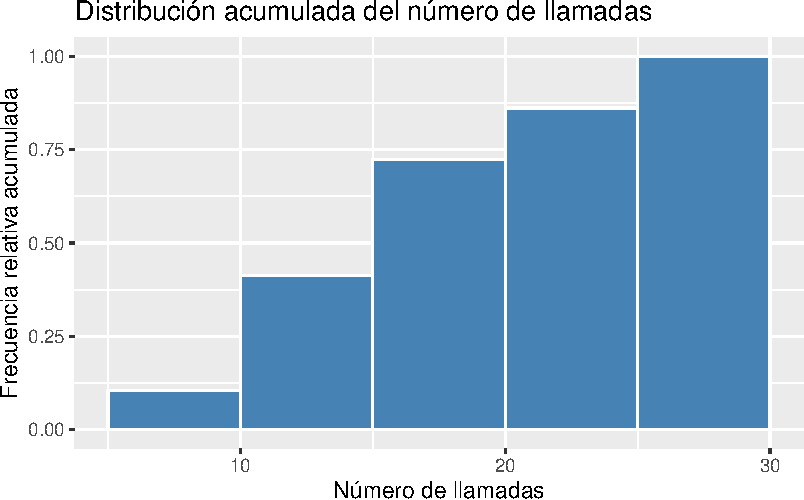
\includegraphics[keepaspectratio]{04-frecuencias-graficos_files/figure-pdf/unnamed-chunk-19-4.pdf}}

  \end{tcolorbox}
\item
  Dibujar el polígono de frecuencias relativas acumuladas (ojiva).

  \begin{tcolorbox}[enhanced jigsaw, breakable, toptitle=1mm, colbacktitle=quarto-callout-tip-color!10!white, rightrule=.15mm, opacityback=0, opacitybacktitle=0.6, titlerule=0mm, coltitle=black, colframe=quarto-callout-tip-color-frame, colback=white, bottomtitle=1mm, leftrule=.75mm, toprule=.15mm, title=\textcolor{quarto-callout-tip-color}{\faLightbulb}\hspace{0.5em}{Solución 1}, arc=.35mm, bottomrule=.15mm, left=2mm]

  Para dibujar la ojiva se puede usar la función
  \href{https://www.rdocumentation.org/packages/graphics/versions/3.6.2/topics/plot}{\texttt{plot}}
  del paquete \texttt{graphics}.

\begin{Shaded}
\begin{Highlighting}[]
\CommentTok{\# Ojiva}
\NormalTok{cortes }\OtherTok{=} \FunctionTok{seq}\NormalTok{(}\DecValTok{5}\NormalTok{, }\DecValTok{30}\NormalTok{, }\DecValTok{5}\NormalTok{)}
\NormalTok{ni }\OtherTok{\textless{}{-}} \FunctionTok{table}\NormalTok{(}\FunctionTok{cut}\NormalTok{(df}\SpecialCharTok{$}\NormalTok{llamadas, }\AttributeTok{breaks =}\NormalTok{ cortes))}
\NormalTok{Fi }\OtherTok{\textless{}{-}} \FunctionTok{c}\NormalTok{(}\DecValTok{0}\NormalTok{, }\FunctionTok{cumsum}\NormalTok{(ni)}\SpecialCharTok{/}\FunctionTok{sum}\NormalTok{(ni))}
\FunctionTok{plot}\NormalTok{(cortes, Fi, }\AttributeTok{type =} \StringTok{"l"}\NormalTok{, }\AttributeTok{col =} \StringTok{"steelblue"}\NormalTok{, }\AttributeTok{main =} \StringTok{"Distribución acumulada del número de llamadas"}\NormalTok{, }\AttributeTok{xlab =} \StringTok{"Número de llamadas"}\NormalTok{, }\AttributeTok{ylab =} \StringTok{"Frecuencia relativa acumulada"}\NormalTok{)}
\end{Highlighting}
\end{Shaded}

  \pandocbounded{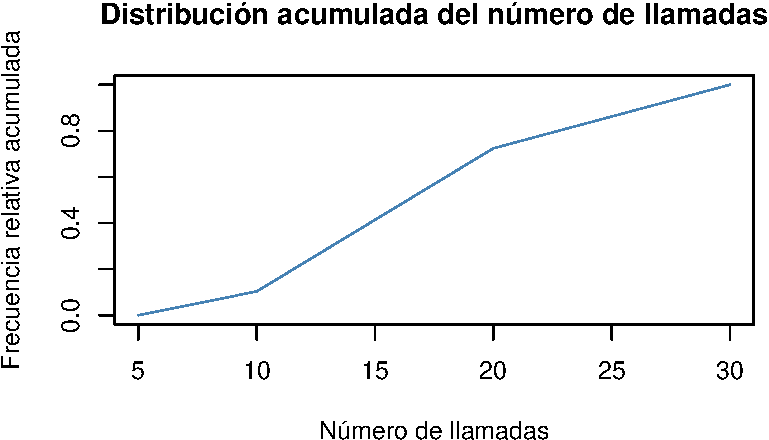
\includegraphics[keepaspectratio]{04-frecuencias-graficos_files/figure-pdf/unnamed-chunk-20-1.pdf}}

  \end{tcolorbox}

  \begin{tcolorbox}[enhanced jigsaw, breakable, toptitle=1mm, colbacktitle=quarto-callout-tip-color!10!white, rightrule=.15mm, opacityback=0, opacitybacktitle=0.6, titlerule=0mm, coltitle=black, colframe=quarto-callout-tip-color-frame, colback=white, bottomtitle=1mm, leftrule=.75mm, toprule=.15mm, title=\textcolor{quarto-callout-tip-color}{\faLightbulb}\hspace{0.5em}{Solución 2}, arc=.35mm, bottomrule=.15mm, left=2mm]

  Otra alternativa es usar la función la función
  \href{https://aprendeconalf.es/manual-r/07-graficos.html\#histogramas}{\texttt{geom\_line}}
  del paquete \texttt{ggplot2}.

\begin{Shaded}
\begin{Highlighting}[]
\FunctionTok{library}\NormalTok{(ggplot2)}
\CommentTok{\# Ojiva}
\NormalTok{cortes }\OtherTok{\textless{}{-}} \FunctionTok{seq}\NormalTok{(}\DecValTok{5}\NormalTok{, }\DecValTok{30}\NormalTok{, }\DecValTok{5}\NormalTok{)}
\NormalTok{tabla\_frec }\OtherTok{\textless{}{-}} \FunctionTok{mutate}\NormalTok{(df, }\AttributeTok{llamadas\_int =} \FunctionTok{cut}\NormalTok{(df}\SpecialCharTok{$}\NormalTok{llamadas, }\AttributeTok{breaks =}\NormalTok{ cortes)) }\SpecialCharTok{|\textgreater{}} 
    \FunctionTok{count}\NormalTok{(llamadas\_int) }\SpecialCharTok{|\textgreater{}}
    \FunctionTok{mutate}\NormalTok{(}\AttributeTok{cortes =}\NormalTok{ cortes[}\SpecialCharTok{{-}}\DecValTok{1}\NormalTok{], }\AttributeTok{Fi =} \FunctionTok{cumsum}\NormalTok{(n)}\SpecialCharTok{/}\FunctionTok{sum}\NormalTok{(n)) }\SpecialCharTok{|\textgreater{}}
    \FunctionTok{select}\NormalTok{(cortes, Fi) }
\NormalTok{tabla\_frec }\OtherTok{\textless{}{-}} \FunctionTok{rbind}\NormalTok{(}\FunctionTok{data.frame}\NormalTok{(}\AttributeTok{cortes =}\NormalTok{ cortes[}\DecValTok{1}\NormalTok{], }\AttributeTok{Fi =} \DecValTok{0}\NormalTok{), tabla\_frec)}
\FunctionTok{ggplot}\NormalTok{(tabla\_frec, }\FunctionTok{aes}\NormalTok{(}\AttributeTok{x =}\NormalTok{ cortes , }\AttributeTok{y =}\NormalTok{ Fi)) }\SpecialCharTok{+}
    \FunctionTok{geom\_line}\NormalTok{(}\AttributeTok{col =} \StringTok{"steelblue"}\NormalTok{) }\SpecialCharTok{+}
    \FunctionTok{labs}\NormalTok{(}\AttributeTok{title =} \StringTok{"Distribución del número de llamadas"}\NormalTok{, }\AttributeTok{x =} \StringTok{"Número de llamadas"}\NormalTok{, }\AttributeTok{y =} \StringTok{"Frecuencia relativa acumulada"}\NormalTok{)}
\end{Highlighting}
\end{Shaded}

  \pandocbounded{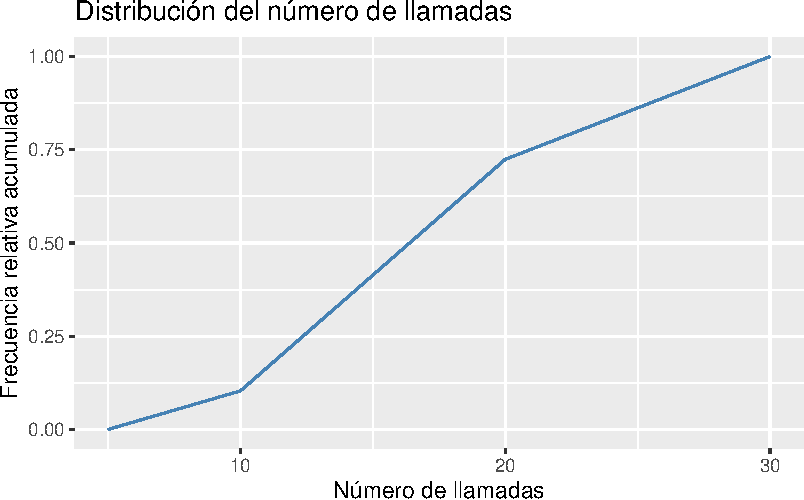
\includegraphics[keepaspectratio]{04-frecuencias-graficos_files/figure-pdf/unnamed-chunk-21-1.pdf}}

  \end{tcolorbox}
\end{enumerate}

\end{exercise}

\begin{exercise}[]\protect\hypertarget{exr-frecuencias-graficos-3}{}\label{exr-frecuencias-graficos-3}

Los grupos sanguíneos de una muestra de 30 personas son:

\begin{longtable}[]{@{}
  >{\centering\arraybackslash}p{(\linewidth - 0\tabcolsep) * \real{1.0000}}@{}}
\toprule\noalign{}
\endhead
\bottomrule\noalign{}
\endlastfoot
A, B, B, A, AB, 0, 0, A, B, B, A, A, A, A, AB, A, A, A, B, 0, B, B, B,
A, A, A, 0, A, AB, 0 \\
\end{longtable}

\begin{enumerate}
\def\labelenumi{\alph{enumi}.}
\item
  Crear un conjunto de datos con la variable \texttt{grupo\_sanguíneo}.

  \begin{tcolorbox}[enhanced jigsaw, breakable, toptitle=1mm, colbacktitle=quarto-callout-tip-color!10!white, rightrule=.15mm, opacityback=0, opacitybacktitle=0.6, titlerule=0mm, coltitle=black, colframe=quarto-callout-tip-color-frame, colback=white, bottomtitle=1mm, leftrule=.75mm, toprule=.15mm, title=\textcolor{quarto-callout-tip-color}{\faLightbulb}\hspace{0.5em}{Solución}, arc=.35mm, bottomrule=.15mm, left=2mm]

\begin{Shaded}
\begin{Highlighting}[]
\NormalTok{df }\OtherTok{\textless{}{-}} \FunctionTok{data.frame}\NormalTok{(}\AttributeTok{grupo\_sanguineo =} \FunctionTok{c}\NormalTok{(}\StringTok{"A"}\NormalTok{, }\StringTok{"B"}\NormalTok{, }\StringTok{"B"}\NormalTok{, }\StringTok{"A"}\NormalTok{, }\StringTok{"AB"}\NormalTok{, }\StringTok{"0"}\NormalTok{, }\StringTok{"0"}\NormalTok{, }\StringTok{"A"}\NormalTok{, }\StringTok{"B"}\NormalTok{, }\StringTok{"B"}\NormalTok{, }\StringTok{"A"}\NormalTok{, }\StringTok{"A"}\NormalTok{, }\StringTok{"A"}\NormalTok{, }\StringTok{"A"}\NormalTok{, }\StringTok{"AB"}\NormalTok{, }\StringTok{"A"}\NormalTok{, }\StringTok{"A"}\NormalTok{, }\StringTok{"A"}\NormalTok{, }\StringTok{"B"}\NormalTok{, }\StringTok{"0"}\NormalTok{, }\StringTok{"B"}\NormalTok{, }\StringTok{"B"}\NormalTok{, }\StringTok{"B"}\NormalTok{, }\StringTok{"A"}\NormalTok{, }\StringTok{"A"}\NormalTok{, }\StringTok{"A"}\NormalTok{, }\StringTok{"0"}\NormalTok{, }\StringTok{"A"}\NormalTok{, }\StringTok{"AB"}\NormalTok{, }\StringTok{"0"}\NormalTok{))}
\end{Highlighting}
\end{Shaded}

  \end{tcolorbox}
\item
  Construir la tabla de frecuencias.

  \begin{tcolorbox}[enhanced jigsaw, breakable, toptitle=1mm, colbacktitle=quarto-callout-tip-color!10!white, rightrule=.15mm, opacityback=0, opacitybacktitle=0.6, titlerule=0mm, coltitle=black, colframe=quarto-callout-tip-color-frame, colback=white, bottomtitle=1mm, leftrule=.75mm, toprule=.15mm, title=\textcolor{quarto-callout-tip-color}{\faLightbulb}\hspace{0.5em}{Solución 1}, arc=.35mm, bottomrule=.15mm, left=2mm]

  Para obtener las frecuencias absolutas se puede usar la función
  \href{https://www.rdocumentation.org/packages/base/versions/3.6.2/topics/table}{\texttt{table}},
  y para las frecuencias relativas la función
  \href{https://www.rdocumentation.org/packages/base/versions/3.6.2/topics/prop.table}{\texttt{prop.table}}
  ambas del paquete base de R.

\begin{Shaded}
\begin{Highlighting}[]
\CommentTok{\# Frecuencias absolutas.}
\NormalTok{ni }\OtherTok{\textless{}{-}} \FunctionTok{table}\NormalTok{(df}\SpecialCharTok{$}\NormalTok{grupo\_sanguineo)}
\CommentTok{\# Frecuencias relativas}
\NormalTok{fi }\OtherTok{\textless{}{-}} \FunctionTok{prop.table}\NormalTok{(ni)}
\NormalTok{tabla\_frec }\OtherTok{\textless{}{-}} \FunctionTok{cbind}\NormalTok{(ni, fi)}
\NormalTok{tabla\_frec}
\end{Highlighting}
\end{Shaded}

\begin{verbatim}
   ni        fi
0   5 0.1666667
A  14 0.4666667
AB  3 0.1000000
B   8 0.2666667
\end{verbatim}

  \end{tcolorbox}

  \begin{tcolorbox}[enhanced jigsaw, breakable, toptitle=1mm, colbacktitle=quarto-callout-tip-color!10!white, rightrule=.15mm, opacityback=0, opacitybacktitle=0.6, titlerule=0mm, coltitle=black, colframe=quarto-callout-tip-color-frame, colback=white, bottomtitle=1mm, leftrule=.75mm, toprule=.15mm, title=\textcolor{quarto-callout-tip-color}{\faLightbulb}\hspace{0.5em}{Solución 2}, arc=.35mm, bottomrule=.15mm, left=2mm]

  Otra alternativa es usar la fución
  \href{https://aprendeconalf.es/manual-r/06-preprocesamiento.html\#conteo-del-n\%C3\%BAmero-de-observaciones}{\texttt{count}}
  del paquete \texttt{dplyr}.

\begin{Shaded}
\begin{Highlighting}[]
\FunctionTok{library}\NormalTok{(dplyr)}
\FunctionTok{library}\NormalTok{(knitr)}
\FunctionTok{library}\NormalTok{(kableExtra)}
\FunctionTok{count}\NormalTok{(df, grupo\_sanguineo) }\SpecialCharTok{|\textgreater{}} 
    \FunctionTok{mutate}\NormalTok{(}\AttributeTok{fi =}\NormalTok{ n}\SpecialCharTok{/}\FunctionTok{sum}\NormalTok{(n)) }\SpecialCharTok{|\textgreater{}}
    \FunctionTok{kable}\NormalTok{()}
\end{Highlighting}
\end{Shaded}

  \begin{longtable}[]{@{}lrr@{}}
  \toprule\noalign{}
  grupo\_sanguineo & n & fi \\
  \midrule\noalign{}
  \endhead
  \bottomrule\noalign{}
  \endlastfoot
  0 & 5 & 0.1666667 \\
  A & 14 & 0.4666667 \\
  AB & 3 & 0.1000000 \\
  B & 8 & 0.2666667 \\
  \end{longtable}

  \end{tcolorbox}
\item
  Dibujar el diagrama de sectores.

  \begin{tcolorbox}[enhanced jigsaw, breakable, toptitle=1mm, colbacktitle=quarto-callout-tip-color!10!white, rightrule=.15mm, opacityback=0, opacitybacktitle=0.6, titlerule=0mm, coltitle=black, colframe=quarto-callout-tip-color-frame, colback=white, bottomtitle=1mm, leftrule=.75mm, toprule=.15mm, title=\textcolor{quarto-callout-tip-color}{\faLightbulb}\hspace{0.5em}{Solución 1}, arc=.35mm, bottomrule=.15mm, left=2mm]

  Para dibujar el diagrama de sectores se puede usar la función
  \href{https://www.rdocumentation.org/packages/graphics/versions/3.6.2/topics/pie}{\texttt{pie}}
  del paquete \texttt{graphics}.

\begin{Shaded}
\begin{Highlighting}[]
\CommentTok{\# Diagrama de sectores}
\FunctionTok{pie}\NormalTok{(ni, }\AttributeTok{col =} \DecValTok{1}\SpecialCharTok{:}\FunctionTok{length}\NormalTok{(ni), }\AttributeTok{main =} \StringTok{"Distribución de los grupos sanguíneos"}\NormalTok{)}
\end{Highlighting}
\end{Shaded}

  \pandocbounded{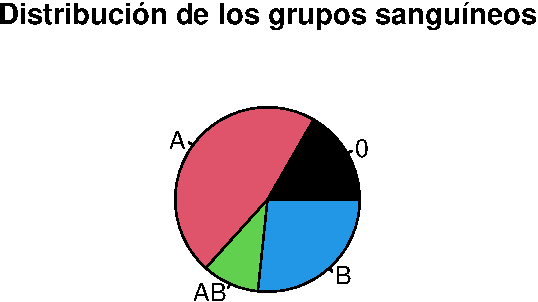
\includegraphics[keepaspectratio]{04-frecuencias-graficos_files/figure-pdf/unnamed-chunk-26-1.pdf}}

  \end{tcolorbox}

  \begin{tcolorbox}[enhanced jigsaw, breakable, toptitle=1mm, colbacktitle=quarto-callout-tip-color!10!white, rightrule=.15mm, opacityback=0, opacitybacktitle=0.6, titlerule=0mm, coltitle=black, colframe=quarto-callout-tip-color-frame, colback=white, bottomtitle=1mm, leftrule=.75mm, toprule=.15mm, title=\textcolor{quarto-callout-tip-color}{\faLightbulb}\hspace{0.5em}{Solución 2}, arc=.35mm, bottomrule=.15mm, left=2mm]

  Otra alternativa es usar las fuciones
  \href{https://aprendeconalf.es/manual-r/07-graficos.html\#diagrama-de-sectores}{\texttt{geom\_bar}}
  y \texttt{coor\_polar} del paquete \texttt{ggplot2}.

\begin{Shaded}
\begin{Highlighting}[]
\FunctionTok{ggplot}\NormalTok{(df, }\FunctionTok{aes}\NormalTok{(}\AttributeTok{x =} \StringTok{""}\NormalTok{, }\AttributeTok{fill =}\NormalTok{ grupo\_sanguineo)) }\SpecialCharTok{+}
    \CommentTok{\# Añadir la capa de las barras.}
    \FunctionTok{geom\_bar}\NormalTok{() }\SpecialCharTok{+}
    \CommentTok{\# Añadir el sistema de coordenadas polares}
    \FunctionTok{coord\_polar}\NormalTok{(}\AttributeTok{theta =} \StringTok{"y"}\NormalTok{) }\SpecialCharTok{+}
    \FunctionTok{labs}\NormalTok{(}\AttributeTok{title =} \StringTok{"Distribución de los grupos sanguíneos"}\NormalTok{)}
\end{Highlighting}
\end{Shaded}

  \pandocbounded{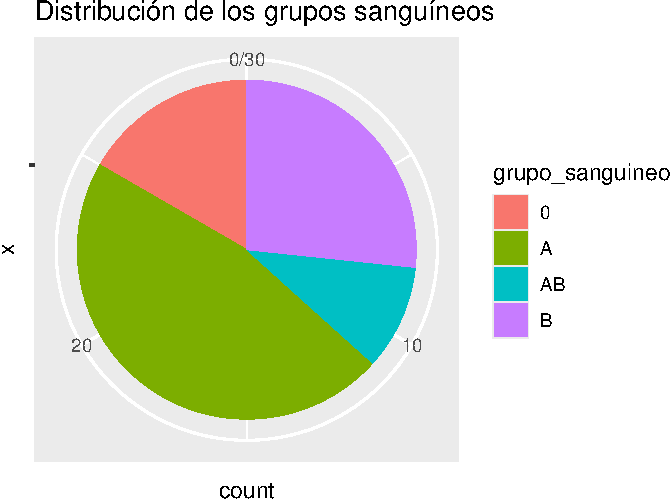
\includegraphics[keepaspectratio]{04-frecuencias-graficos_files/figure-pdf/unnamed-chunk-27-1.pdf}}

  \end{tcolorbox}
\end{enumerate}

\end{exercise}

\begin{exercise}[]\protect\hypertarget{exr-frecuencias-graficos-4}{}\label{exr-frecuencias-graficos-4}

En un estudio de población se tomó una muestra de 27 personas, y se les
preguntó por su edad y estado civil, obteniendo los siguientes
resultados:

\begin{longtable}[]{@{}ll@{}}
\toprule\noalign{}
Estado civil & Edad \\
\midrule\noalign{}
\endhead
\bottomrule\noalign{}
\endlastfoot
Soltero & 31, 45, 35, 65, 21, 38, 62, 22, 31 \\
Casado & 62, 39, 62, 59, 21, 62 \\
Viudo & 80, 68, 65, 40, 78, 69, 75 \\
Divorciado & 31, 65, 59, 49, 65 \\
\end{longtable}

\begin{enumerate}
\def\labelenumi{\alph{enumi}.}
\item
  Crear un conjunto de datos con la variables \texttt{estado\_civil} y
  \texttt{edad}.

  \begin{tcolorbox}[enhanced jigsaw, breakable, toptitle=1mm, colbacktitle=quarto-callout-tip-color!10!white, rightrule=.15mm, opacityback=0, opacitybacktitle=0.6, titlerule=0mm, coltitle=black, colframe=quarto-callout-tip-color-frame, colback=white, bottomtitle=1mm, leftrule=.75mm, toprule=.15mm, title=\textcolor{quarto-callout-tip-color}{\faLightbulb}\hspace{0.5em}{Solución}, arc=.35mm, bottomrule=.15mm, left=2mm]

\begin{Shaded}
\begin{Highlighting}[]
\NormalTok{df }\OtherTok{\textless{}{-}} \FunctionTok{data.frame}\NormalTok{(}
    \AttributeTok{edad =} \FunctionTok{c}\NormalTok{(}\DecValTok{31}\NormalTok{, }\DecValTok{45}\NormalTok{, }\DecValTok{35}\NormalTok{, }\DecValTok{65}\NormalTok{, }\DecValTok{21}\NormalTok{, }\DecValTok{38}\NormalTok{, }\DecValTok{62}\NormalTok{, }\DecValTok{22}\NormalTok{, }\DecValTok{31}\NormalTok{, }\DecValTok{62}\NormalTok{, }\DecValTok{39}\NormalTok{, }\DecValTok{62}\NormalTok{, }\DecValTok{59}\NormalTok{, }\DecValTok{21}\NormalTok{, }\DecValTok{62}\NormalTok{, }\DecValTok{80}\NormalTok{, }\DecValTok{68}\NormalTok{, }\DecValTok{65}\NormalTok{, }\DecValTok{40}\NormalTok{, }\DecValTok{78}\NormalTok{, }\DecValTok{69}\NormalTok{, }\DecValTok{75}\NormalTok{, }\DecValTok{31}\NormalTok{, }\DecValTok{65}\NormalTok{, }\DecValTok{59}\NormalTok{, }\DecValTok{49}\NormalTok{, }\DecValTok{65}\NormalTok{), }
    \AttributeTok{estado\_civil =} \FunctionTok{rep}\NormalTok{(}\FunctionTok{c}\NormalTok{(}\StringTok{"Soltero"}\NormalTok{, }\StringTok{"Casado"}\NormalTok{, }\StringTok{"Viudo"}\NormalTok{, }\StringTok{"Divorciado"}\NormalTok{), }\FunctionTok{c}\NormalTok{(}\DecValTok{9}\NormalTok{, }\DecValTok{6}\NormalTok{, }\DecValTok{7}\NormalTok{, }\DecValTok{5}\NormalTok{)))}
\end{Highlighting}
\end{Shaded}

  \end{tcolorbox}
\item
  Calcular los tamaños muestrales según \texttt{estado\_civil}.

  \begin{tcolorbox}[enhanced jigsaw, breakable, toptitle=1mm, colbacktitle=quarto-callout-tip-color!10!white, rightrule=.15mm, opacityback=0, opacitybacktitle=0.6, titlerule=0mm, coltitle=black, colframe=quarto-callout-tip-color-frame, colback=white, bottomtitle=1mm, leftrule=.75mm, toprule=.15mm, title=\textcolor{quarto-callout-tip-color}{\faLightbulb}\hspace{0.5em}{Solución 1}, arc=.35mm, bottomrule=.15mm, left=2mm]

  Usando la función \texttt{table} del paquete base de R podemos obtener
  las frecuencias absolutas del estado civil que es el tamaño muestral
  de cada grupo.

\begin{Shaded}
\begin{Highlighting}[]
\FunctionTok{table}\NormalTok{(df}\SpecialCharTok{$}\NormalTok{estado\_civil)}
\end{Highlighting}
\end{Shaded}

\begin{verbatim}

    Casado Divorciado    Soltero      Viudo 
         6          5          9          7 
\end{verbatim}

  \end{tcolorbox}

  \begin{tcolorbox}[enhanced jigsaw, breakable, toptitle=1mm, colbacktitle=quarto-callout-tip-color!10!white, rightrule=.15mm, opacityback=0, opacitybacktitle=0.6, titlerule=0mm, coltitle=black, colframe=quarto-callout-tip-color-frame, colback=white, bottomtitle=1mm, leftrule=.75mm, toprule=.15mm, title=\textcolor{quarto-callout-tip-color}{\faLightbulb}\hspace{0.5em}{Solución 2}, arc=.35mm, bottomrule=.15mm, left=2mm]

  Usando las funciones \texttt{groub\_by}, \texttt{summarise} y
  \texttt{n} del paquete \texttt{dplyr}.

\begin{Shaded}
\begin{Highlighting}[]
\FunctionTok{library}\NormalTok{(dplyr)}
\NormalTok{df }\SpecialCharTok{|\textgreater{}} \FunctionTok{group\_by}\NormalTok{(estado\_civil) }\SpecialCharTok{|\textgreater{}}
    \FunctionTok{summarise}\NormalTok{(}\AttributeTok{n =} \FunctionTok{n}\NormalTok{())}
\end{Highlighting}
\end{Shaded}

\begin{verbatim}
# A tibble: 4 x 2
  estado_civil     n
  <chr>        <int>
1 Casado           6
2 Divorciado       5
3 Soltero          9
4 Viudo            7
\end{verbatim}

  \end{tcolorbox}
\item
  Construir la tabla de frecuencias de la variable \texttt{edad} para
  cada categoría de la variable \texttt{estado\_civil}.

  \begin{tcolorbox}[enhanced jigsaw, breakable, toptitle=1mm, colbacktitle=quarto-callout-tip-color!10!white, rightrule=.15mm, opacityback=0, opacitybacktitle=0.6, titlerule=0mm, coltitle=black, colframe=quarto-callout-tip-color-frame, colback=white, bottomtitle=1mm, leftrule=.75mm, toprule=.15mm, title=\textcolor{quarto-callout-tip-color}{\faLightbulb}\hspace{0.5em}{Solución}, arc=.35mm, bottomrule=.15mm, left=2mm]

  Para dividir la muestra en grupos se puede usar la función
  \href{https://aprendeconalf.es/manual-r/06-preprocesamiento.html\#res\%C3\%BAmenes-por-grupos}{\texttt{group-by}}
  del paquete \texttt{dplyr}.

\begin{Shaded}
\begin{Highlighting}[]
\FunctionTok{library}\NormalTok{(dplyr)}
\FunctionTok{library}\NormalTok{(knitr)}
\FunctionTok{library}\NormalTok{(kableExtra)}
\FunctionTok{mutate}\NormalTok{(df, }\AttributeTok{edad\_int =} \FunctionTok{cut}\NormalTok{(edad, }\AttributeTok{breaks =} \FunctionTok{seq}\NormalTok{(}\DecValTok{20}\NormalTok{, }\DecValTok{80}\NormalTok{, }\DecValTok{10}\NormalTok{))) }\SpecialCharTok{|\textgreater{}}
    \FunctionTok{group\_by}\NormalTok{(estado\_civil) }\SpecialCharTok{|\textgreater{}}
    \FunctionTok{count}\NormalTok{(edad\_int) }\SpecialCharTok{|\textgreater{}} 
    \FunctionTok{mutate}\NormalTok{(}\AttributeTok{fi =}\NormalTok{ n}\SpecialCharTok{/}\FunctionTok{sum}\NormalTok{(n), }\AttributeTok{Ni =} \FunctionTok{cumsum}\NormalTok{(n), }\AttributeTok{Fi =} \FunctionTok{cumsum}\NormalTok{(n)}\SpecialCharTok{/}\FunctionTok{sum}\NormalTok{(n)) }\SpecialCharTok{|\textgreater{}}
    \FunctionTok{kable}\NormalTok{()}
\end{Highlighting}
\end{Shaded}

  \begin{longtable}[]{@{}llrrrr@{}}
  \toprule\noalign{}
  estado\_civil & edad\_int & n & fi & Ni & Fi \\
  \midrule\noalign{}
  \endhead
  \bottomrule\noalign{}
  \endlastfoot
  Casado & (20,30{]} & 1 & 0.1666667 & 1 & 0.1666667 \\
  Casado & (30,40{]} & 1 & 0.1666667 & 2 & 0.3333333 \\
  Casado & (50,60{]} & 1 & 0.1666667 & 3 & 0.5000000 \\
  Casado & (60,70{]} & 3 & 0.5000000 & 6 & 1.0000000 \\
  Divorciado & (30,40{]} & 1 & 0.2000000 & 1 & 0.2000000 \\
  Divorciado & (40,50{]} & 1 & 0.2000000 & 2 & 0.4000000 \\
  Divorciado & (50,60{]} & 1 & 0.2000000 & 3 & 0.6000000 \\
  Divorciado & (60,70{]} & 2 & 0.4000000 & 5 & 1.0000000 \\
  Soltero & (20,30{]} & 2 & 0.2222222 & 2 & 0.2222222 \\
  Soltero & (30,40{]} & 4 & 0.4444444 & 6 & 0.6666667 \\
  Soltero & (40,50{]} & 1 & 0.1111111 & 7 & 0.7777778 \\
  Soltero & (60,70{]} & 2 & 0.2222222 & 9 & 1.0000000 \\
  Viudo & (30,40{]} & 1 & 0.1428571 & 1 & 0.1428571 \\
  Viudo & (60,70{]} & 3 & 0.4285714 & 4 & 0.5714286 \\
  Viudo & (70,80{]} & 3 & 0.4285714 & 7 & 1.0000000 \\
  \end{longtable}

  \end{tcolorbox}
\item
  Dibujar los diagramas de cajas de la edad según el estado civil.
  ¿Existen datos atípicos? ¿En qué grupo hay mayor dispersión?

  \begin{tcolorbox}[enhanced jigsaw, breakable, toptitle=1mm, colbacktitle=quarto-callout-tip-color!10!white, rightrule=.15mm, opacityback=0, opacitybacktitle=0.6, titlerule=0mm, coltitle=black, colframe=quarto-callout-tip-color-frame, colback=white, bottomtitle=1mm, leftrule=.75mm, toprule=.15mm, title=\textcolor{quarto-callout-tip-color}{\faLightbulb}\hspace{0.5em}{Solución}, arc=.35mm, bottomrule=.15mm, left=2mm]

\begin{Shaded}
\begin{Highlighting}[]
\FunctionTok{library}\NormalTok{(ggplot2)}
\FunctionTok{ggplot}\NormalTok{(df, }\FunctionTok{aes}\NormalTok{(}\AttributeTok{x =}\NormalTok{ edad, }\AttributeTok{fill =}\NormalTok{ estado\_civil)) }\SpecialCharTok{+}
    \FunctionTok{geom\_boxplot}\NormalTok{()}
\end{Highlighting}
\end{Shaded}

  \pandocbounded{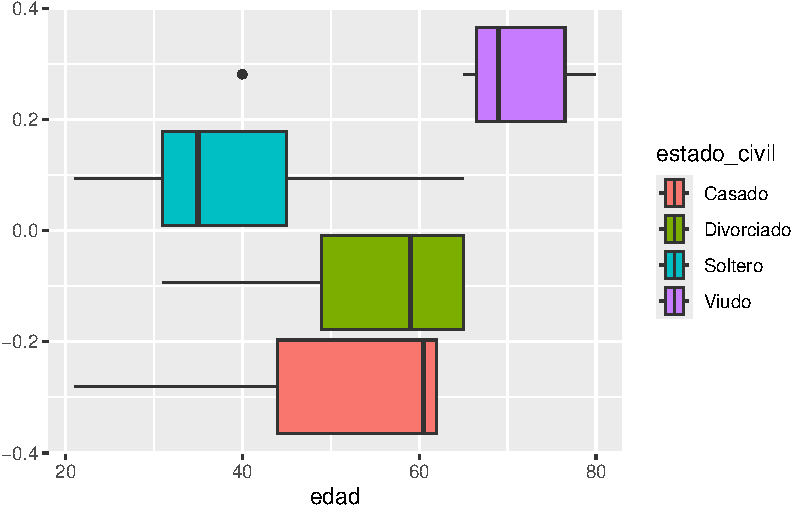
\includegraphics[keepaspectratio]{04-frecuencias-graficos_files/figure-pdf/unnamed-chunk-33-1.pdf}}

  \end{tcolorbox}
\item
  Dibujar los histogramas de la edad según el estado civil.

  \begin{tcolorbox}[enhanced jigsaw, breakable, toptitle=1mm, colbacktitle=quarto-callout-tip-color!10!white, rightrule=.15mm, opacityback=0, opacitybacktitle=0.6, titlerule=0mm, coltitle=black, colframe=quarto-callout-tip-color-frame, colback=white, bottomtitle=1mm, leftrule=.75mm, toprule=.15mm, title=\textcolor{quarto-callout-tip-color}{\faLightbulb}\hspace{0.5em}{Solución}, arc=.35mm, bottomrule=.15mm, left=2mm]

\begin{Shaded}
\begin{Highlighting}[]
\FunctionTok{ggplot}\NormalTok{(df, }\FunctionTok{aes}\NormalTok{(}\AttributeTok{x =}\NormalTok{ edad, }\AttributeTok{fill =}\NormalTok{ estado\_civil)) }\SpecialCharTok{+}
    \FunctionTok{geom\_histogram}\NormalTok{(}\AttributeTok{breaks =} \FunctionTok{seq}\NormalTok{(}\DecValTok{20}\NormalTok{, }\DecValTok{80}\NormalTok{, }\DecValTok{10}\NormalTok{), }\AttributeTok{position =} \StringTok{"identity"}\NormalTok{, }\AttributeTok{alpha=}\FloatTok{0.4}\NormalTok{)}
\end{Highlighting}
\end{Shaded}

  \pandocbounded{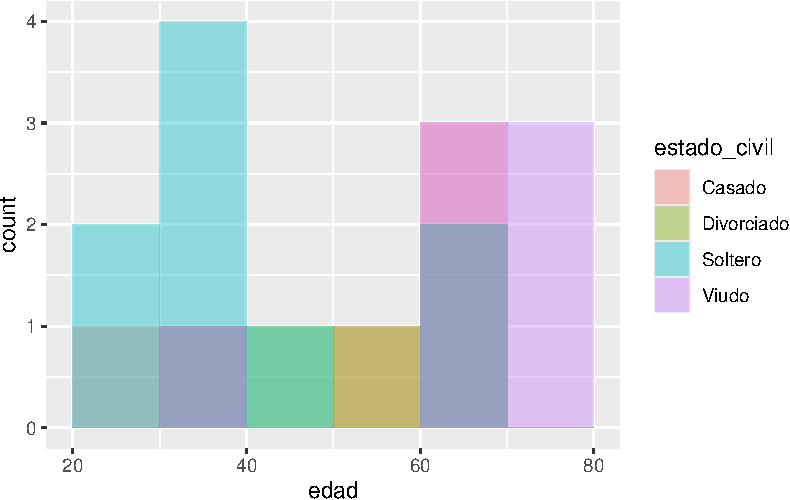
\includegraphics[keepaspectratio]{04-frecuencias-graficos_files/figure-pdf/unnamed-chunk-34-1.pdf}}

  Para dibujar cada histograma por separado se puede usar la función
  \href{https://aprendeconalf.es/manual-r/07-graficos.html\#facetas}{\texttt{facet\_wrap}}
  o \texttt{facet\_grid} del paquete \texttt{ggplot2}.

\begin{Shaded}
\begin{Highlighting}[]
\FunctionTok{ggplot}\NormalTok{(df, }\FunctionTok{aes}\NormalTok{(}\AttributeTok{x =}\NormalTok{ edad, }\AttributeTok{fill =}\NormalTok{ estado\_civil)) }\SpecialCharTok{+}
    \FunctionTok{geom\_histogram}\NormalTok{(}\AttributeTok{breaks =} \FunctionTok{seq}\NormalTok{(}\DecValTok{20}\NormalTok{, }\DecValTok{80}\NormalTok{, }\DecValTok{10}\NormalTok{)) }\SpecialCharTok{+}
    \CommentTok{\# Añadir la faceta del estado civil}
    \FunctionTok{facet\_grid}\NormalTok{(}\AttributeTok{rows =} \FunctionTok{vars}\NormalTok{(estado\_civil))}
\end{Highlighting}
\end{Shaded}

  \pandocbounded{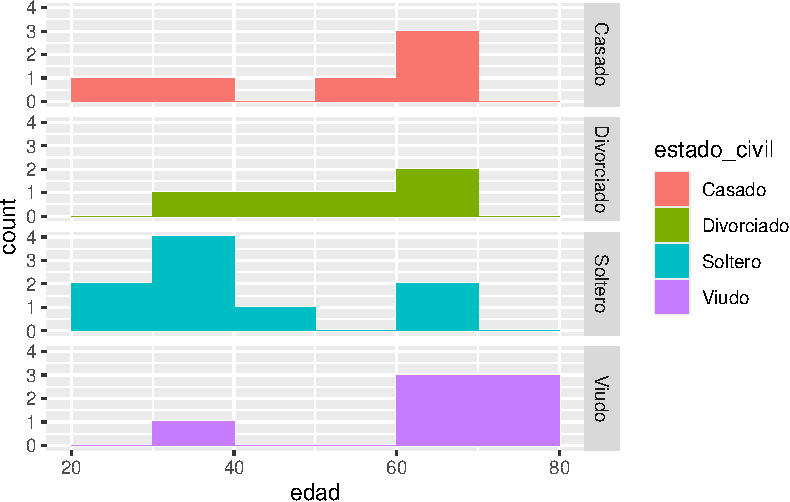
\includegraphics[keepaspectratio]{04-frecuencias-graficos_files/figure-pdf/unnamed-chunk-35-1.pdf}}

  \end{tcolorbox}
\end{enumerate}

\end{exercise}

\section{Ejercicios propuestos}\label{ejercicios-propuestos-2}

\begin{exercise}[]\protect\hypertarget{exr-frecuencias-graficos-5}{}\label{exr-frecuencias-graficos-5}

El conjunto de datos \href{datos/neonatos.csv}{neonatos} contiene
información sobre una muestra de 320 recién nacidos en un hospital
durante un año que cumplieron el tiempo normal de gestación.

\begin{enumerate}
\def\labelenumi{\alph{enumi}.}
\item
  Construir la tabla de frecuencias de la puntuación Apgar al minuto de
  nacer. Si se considera que una puntuación Apgar de 3 o menos indica
  que el neonato está deprimido, ¿qué porcentaje de niños está deprimido
  en la muestra?
\item
  Comparar las distribuciones de frecuencias de las puntuaciones Apgar
  al minuto de nacer según si la madre es mayor o menor de 20 años. ¿En
  qué grupo hay más neonatos deprimidos?
\item
  Construir la tabla de frecuencias para el peso de los neonatos,
  agrupando en clases de amplitud \(0.5\) desde el \(2\) hasta el
  \(4.5\). ¿En qué intervalo de peso hay más neonatos?
\item
  Comparar la distribución de frecuencias relativas del peso de los
  neonatos según si la madre fuma o no. Si se considera como peso bajo
  un peso menor de \(2.5\) kg, ¿En qué grupo hay un mayor porcentaje de
  niños con peso bajo?
\item
  Construir el diagrama de barras de la puntuación Apgar al minuto. ¿Qué
  puntuación Apgar es la más frecuente?
\item
  Construir el diagrama de frecuencias relativas acumuladas de la
  puntuación Apgar al minuto. ¿Por debajo de que puntuación estarán la
  mitad de los niños?
\item
  Comparar mediante diagramas de barras de frecuencias relativas las
  distribuciones de las puntuaciones Apgar al minuto según si la madre
  ha fumado o no durante el embarazo. ¿Qué se puede concluir?
\item
  Construir el histograma de pesos, agrupando en clases de amplitud
  \(0.5\) desde el \(2\) hasta el \(4.5\). ¿En qué intervalo de peso hay
  más niños?
\item
  Comparar la distribución de frecuencias relativas del peso de los
  neonatos según si la madre fuma o no. ¿En qué grupo se aprecia menor
  peso de los niños de la muestra?
\item
  Comparar la distribución de frecuencias relativas del peso de los
  neonatos según si la madre fumaba o no antes del embarazo. ¿Qué se
  puede concluir?
\item
  Construir el diagrama de caja y bigotes del peso. ¿Entre qué valores
  se considera que el peso de un neonato es normal? ¿Existen datos
  atípicos?
\item
  Comparar el diagrama de cajas y bigotes del peso, según si la madre
  fumó o no durante el embarazo y si era mayor o no de 20 años. ¿En qué
  grupo el peso tiene más dispersión central? ¿En qué grupo pesan menos
  los niños de la muestra?
\item
  Comparar el diagrama de cajas de la puntuación Apgar al minuto y a los
  cinco minutos. ¿En qué variable hay más dispersión central?
\end{enumerate}

\end{exercise}

\bookmarksetup{startatroot}

\chapter{Estadística Descriptiva}\label{estaduxedstica-descriptiva}

\section{Ejercicios Resueltos}\label{ejercicios-resueltos-3}

Para la realización de esta práctica se requieren los siguientes
paquetes:

\begin{Shaded}
\begin{Highlighting}[]
\FunctionTok{library}\NormalTok{(tidyverse) }
\CommentTok{\# Incluye los siguientes paquetes:}
\CommentTok{\# {-} readr: para la lectura de ficheros csv. }
\CommentTok{\# {-} dplyr: para el preprocesamiento y manipulación de datos.}
\FunctionTok{library}\NormalTok{(vtable) }\CommentTok{\# para resúmenes estadísticos.}
\FunctionTok{library}\NormalTok{(skimr) }\CommentTok{\# para resúmenes estadísticos.}
\FunctionTok{library}\NormalTok{(summarytools) }\CommentTok{\# para resúmenes estadísticos.}
\FunctionTok{library}\NormalTok{(knitr) }\CommentTok{\# para el formateo de tablas.}
\FunctionTok{library}\NormalTok{(kableExtra) }\CommentTok{\# para personalizar el formato de las tablas.}
\end{Highlighting}
\end{Shaded}

\begin{exercise}[]\protect\hypertarget{exr-descriptiva-1}{}\label{exr-descriptiva-1}

En una encuesta a 25 matrimonios sobre el número de hijos que tenían se
obtuvieron los siguientes datos:

\begin{longtable}[]{@{}
  >{\centering\arraybackslash}p{(\linewidth - 0\tabcolsep) * \real{1.0000}}@{}}
\toprule\noalign{}
\endhead
\bottomrule\noalign{}
\endlastfoot
1, 2, 4, 2, 2, 2, 3, 2, 1, 1, 0, 2, 2, 0, 2, 2, 1, 2, 2, 3, 1, 2, 2, 1,
2 \\
\end{longtable}

\begin{enumerate}
\def\labelenumi{\alph{enumi}.}
\item
  Crear un conjunto de datos con la variable \texttt{hijos}.

  \begin{tcolorbox}[enhanced jigsaw, breakable, toptitle=1mm, colbacktitle=quarto-callout-tip-color!10!white, rightrule=.15mm, opacityback=0, opacitybacktitle=0.6, titlerule=0mm, coltitle=black, colframe=quarto-callout-tip-color-frame, colback=white, bottomtitle=1mm, leftrule=.75mm, toprule=.15mm, title=\textcolor{quarto-callout-tip-color}{\faLightbulb}\hspace{0.5em}{Solución}, arc=.35mm, bottomrule=.15mm, left=2mm]

\begin{Shaded}
\begin{Highlighting}[]
\NormalTok{df }\OtherTok{\textless{}{-}} \FunctionTok{data.frame}\NormalTok{(}\AttributeTok{hijos =} \FunctionTok{c}\NormalTok{(}\DecValTok{1}\NormalTok{, }\DecValTok{2}\NormalTok{, }\DecValTok{4}\NormalTok{, }\DecValTok{2}\NormalTok{, }\DecValTok{2}\NormalTok{, }\DecValTok{2}\NormalTok{, }\DecValTok{3}\NormalTok{, }\DecValTok{2}\NormalTok{, }\DecValTok{1}\NormalTok{, }\DecValTok{1}\NormalTok{, }\DecValTok{0}\NormalTok{, }\DecValTok{2}\NormalTok{, }\DecValTok{2}\NormalTok{, }\DecValTok{0}\NormalTok{, }\DecValTok{2}\NormalTok{, }\DecValTok{2}\NormalTok{, }\DecValTok{1}\NormalTok{, }\DecValTok{2}\NormalTok{, }\DecValTok{2}\NormalTok{, }\DecValTok{3}\NormalTok{, }\DecValTok{1}\NormalTok{, }\DecValTok{2}\NormalTok{, }\DecValTok{2}\NormalTok{, }\DecValTok{1}\NormalTok{, }\DecValTok{2}\NormalTok{))}
\end{Highlighting}
\end{Shaded}

  \end{tcolorbox}
\item
  Calcular el tamaño muestral.

  \begin{tcolorbox}[enhanced jigsaw, breakable, toptitle=1mm, colbacktitle=quarto-callout-tip-color!10!white, rightrule=.15mm, opacityback=0, opacitybacktitle=0.6, titlerule=0mm, coltitle=black, colframe=quarto-callout-tip-color-frame, colback=white, bottomtitle=1mm, leftrule=.75mm, toprule=.15mm, title=\textcolor{quarto-callout-tip-color}{\faLightbulb}\hspace{0.5em}{Solución}, arc=.35mm, bottomrule=.15mm, left=2mm]

\begin{Shaded}
\begin{Highlighting}[]
\FunctionTok{nrow}\NormalTok{(df)}
\end{Highlighting}
\end{Shaded}

\begin{verbatim}
[1] 25
\end{verbatim}

  \end{tcolorbox}
\item
  Calcular la media.

  \begin{tcolorbox}[enhanced jigsaw, breakable, toptitle=1mm, colbacktitle=quarto-callout-tip-color!10!white, rightrule=.15mm, opacityback=0, opacitybacktitle=0.6, titlerule=0mm, coltitle=black, colframe=quarto-callout-tip-color-frame, colback=white, bottomtitle=1mm, leftrule=.75mm, toprule=.15mm, title=\textcolor{quarto-callout-tip-color}{\faLightbulb}\hspace{0.5em}{Solución}, arc=.35mm, bottomrule=.15mm, left=2mm]

\begin{Shaded}
\begin{Highlighting}[]
\FunctionTok{mean}\NormalTok{(df}\SpecialCharTok{$}\NormalTok{hijos)}
\end{Highlighting}
\end{Shaded}

\begin{verbatim}
[1] 1.76
\end{verbatim}

  \end{tcolorbox}
\item
  Calcular la mediana.

  \begin{tcolorbox}[enhanced jigsaw, breakable, toptitle=1mm, colbacktitle=quarto-callout-tip-color!10!white, rightrule=.15mm, opacityback=0, opacitybacktitle=0.6, titlerule=0mm, coltitle=black, colframe=quarto-callout-tip-color-frame, colback=white, bottomtitle=1mm, leftrule=.75mm, toprule=.15mm, title=\textcolor{quarto-callout-tip-color}{\faLightbulb}\hspace{0.5em}{Solución}, arc=.35mm, bottomrule=.15mm, left=2mm]

\begin{Shaded}
\begin{Highlighting}[]
\FunctionTok{median}\NormalTok{(df}\SpecialCharTok{$}\NormalTok{hijos)}
\end{Highlighting}
\end{Shaded}

\begin{verbatim}
[1] 2
\end{verbatim}

  \end{tcolorbox}
\item
  Calcular la moda.

  \begin{tcolorbox}[enhanced jigsaw, breakable, toptitle=1mm, colbacktitle=quarto-callout-tip-color!10!white, rightrule=.15mm, opacityback=0, opacitybacktitle=0.6, titlerule=0mm, coltitle=black, colframe=quarto-callout-tip-color-frame, colback=white, bottomtitle=1mm, leftrule=.75mm, toprule=.15mm, title=\textcolor{quarto-callout-tip-color}{\faLightbulb}\hspace{0.5em}{Solución}, arc=.35mm, bottomrule=.15mm, left=2mm]

  El paquete base de R no tiene implementada ninguna función para
  calcular la moda, así que definiremos nuestra propia función.

\begin{Shaded}
\begin{Highlighting}[]
\NormalTok{moda }\OtherTok{\textless{}{-}} \ControlFlowTok{function}\NormalTok{(x) \{}
\NormalTok{u }\OtherTok{\textless{}{-}} \FunctionTok{unique}\NormalTok{(x) }\CommentTok{\# Vector con los valores de la muestra sin repetir (sin ordenar).}
\NormalTok{tab }\OtherTok{\textless{}{-}} \FunctionTok{tabulate}\NormalTok{(}\FunctionTok{match}\NormalTok{(x, u)) }\CommentTok{\# Frecuencias absolutas de los valores en u.}
\NormalTok{u[tab }\SpecialCharTok{==} \FunctionTok{max}\NormalTok{(tab)] }\CommentTok{\# Valor con la mayor frecuencia.}
\NormalTok{\}}

\FunctionTok{moda}\NormalTok{(df}\SpecialCharTok{$}\NormalTok{hijos)}
\end{Highlighting}
\end{Shaded}

\begin{verbatim}
[1] 2
\end{verbatim}

  \end{tcolorbox}
\item
  Calcular el mínimo.

  \begin{tcolorbox}[enhanced jigsaw, breakable, toptitle=1mm, colbacktitle=quarto-callout-tip-color!10!white, rightrule=.15mm, opacityback=0, opacitybacktitle=0.6, titlerule=0mm, coltitle=black, colframe=quarto-callout-tip-color-frame, colback=white, bottomtitle=1mm, leftrule=.75mm, toprule=.15mm, title=\textcolor{quarto-callout-tip-color}{\faLightbulb}\hspace{0.5em}{Solución}, arc=.35mm, bottomrule=.15mm, left=2mm]

\begin{Shaded}
\begin{Highlighting}[]
\FunctionTok{min}\NormalTok{(df}\SpecialCharTok{$}\NormalTok{hijos)}
\end{Highlighting}
\end{Shaded}

\begin{verbatim}
[1] 0
\end{verbatim}

  \end{tcolorbox}
\item
  Calcular el máximo.

  \begin{tcolorbox}[enhanced jigsaw, breakable, toptitle=1mm, colbacktitle=quarto-callout-tip-color!10!white, rightrule=.15mm, opacityback=0, opacitybacktitle=0.6, titlerule=0mm, coltitle=black, colframe=quarto-callout-tip-color-frame, colback=white, bottomtitle=1mm, leftrule=.75mm, toprule=.15mm, title=\textcolor{quarto-callout-tip-color}{\faLightbulb}\hspace{0.5em}{Solución}, arc=.35mm, bottomrule=.15mm, left=2mm]

\begin{Shaded}
\begin{Highlighting}[]
\FunctionTok{max}\NormalTok{(df}\SpecialCharTok{$}\NormalTok{hijos)}
\end{Highlighting}
\end{Shaded}

\begin{verbatim}
[1] 4
\end{verbatim}

  \end{tcolorbox}
\item
  Calcular los cuartiles.

  \begin{tcolorbox}[enhanced jigsaw, breakable, toptitle=1mm, colbacktitle=quarto-callout-tip-color!10!white, rightrule=.15mm, opacityback=0, opacitybacktitle=0.6, titlerule=0mm, coltitle=black, colframe=quarto-callout-tip-color-frame, colback=white, bottomtitle=1mm, leftrule=.75mm, toprule=.15mm, title=\textcolor{quarto-callout-tip-color}{\faLightbulb}\hspace{0.5em}{Solución}, arc=.35mm, bottomrule=.15mm, left=2mm]

\begin{Shaded}
\begin{Highlighting}[]
\FunctionTok{quantile}\NormalTok{(df}\SpecialCharTok{$}\NormalTok{hijos, }\AttributeTok{prob=}\FunctionTok{c}\NormalTok{(}\FloatTok{0.25}\NormalTok{, }\FloatTok{0.5}\NormalTok{, }\FloatTok{0.75}\NormalTok{))}
\end{Highlighting}
\end{Shaded}

\begin{verbatim}
25% 50% 75% 
  1   2   2 
\end{verbatim}

  \end{tcolorbox}
\item
  Calcular los percentiles 5 y 95.

  \begin{tcolorbox}[enhanced jigsaw, breakable, toptitle=1mm, colbacktitle=quarto-callout-tip-color!10!white, rightrule=.15mm, opacityback=0, opacitybacktitle=0.6, titlerule=0mm, coltitle=black, colframe=quarto-callout-tip-color-frame, colback=white, bottomtitle=1mm, leftrule=.75mm, toprule=.15mm, title=\textcolor{quarto-callout-tip-color}{\faLightbulb}\hspace{0.5em}{Solución}, arc=.35mm, bottomrule=.15mm, left=2mm]

\begin{Shaded}
\begin{Highlighting}[]
\FunctionTok{quantile}\NormalTok{(df}\SpecialCharTok{$}\NormalTok{hijos, }\AttributeTok{prob=}\FunctionTok{c}\NormalTok{(}\FloatTok{0.05}\NormalTok{, }\FloatTok{0.95}\NormalTok{))}
\end{Highlighting}
\end{Shaded}

\begin{verbatim}
 5% 95% 
0.2 3.0 
\end{verbatim}

  \end{tcolorbox}
\item
  Calcular el rango.

  \begin{tcolorbox}[enhanced jigsaw, breakable, toptitle=1mm, colbacktitle=quarto-callout-tip-color!10!white, rightrule=.15mm, opacityback=0, opacitybacktitle=0.6, titlerule=0mm, coltitle=black, colframe=quarto-callout-tip-color-frame, colback=white, bottomtitle=1mm, leftrule=.75mm, toprule=.15mm, title=\textcolor{quarto-callout-tip-color}{\faLightbulb}\hspace{0.5em}{Solución}, arc=.35mm, bottomrule=.15mm, left=2mm]

\begin{Shaded}
\begin{Highlighting}[]
\FunctionTok{max}\NormalTok{(df}\SpecialCharTok{$}\NormalTok{hijos) }\SpecialCharTok{{-}} \FunctionTok{min}\NormalTok{(df}\SpecialCharTok{$}\NormalTok{hijos)}
\end{Highlighting}
\end{Shaded}

\begin{verbatim}
[1] 4
\end{verbatim}

  \end{tcolorbox}
\item
  Calcular el rango intecuartílico.

  \begin{tcolorbox}[enhanced jigsaw, breakable, toptitle=1mm, colbacktitle=quarto-callout-tip-color!10!white, rightrule=.15mm, opacityback=0, opacitybacktitle=0.6, titlerule=0mm, coltitle=black, colframe=quarto-callout-tip-color-frame, colback=white, bottomtitle=1mm, leftrule=.75mm, toprule=.15mm, title=\textcolor{quarto-callout-tip-color}{\faLightbulb}\hspace{0.5em}{Solución}, arc=.35mm, bottomrule=.15mm, left=2mm]

\begin{Shaded}
\begin{Highlighting}[]
\FunctionTok{IQR}\NormalTok{(df}\SpecialCharTok{$}\NormalTok{hijos)}
\end{Highlighting}
\end{Shaded}

\begin{verbatim}
[1] 1
\end{verbatim}

  \end{tcolorbox}
\item
  Calcular la varianza

  \begin{tcolorbox}[enhanced jigsaw, breakable, toptitle=1mm, colbacktitle=quarto-callout-tip-color!10!white, rightrule=.15mm, opacityback=0, opacitybacktitle=0.6, titlerule=0mm, coltitle=black, colframe=quarto-callout-tip-color-frame, colback=white, bottomtitle=1mm, leftrule=.75mm, toprule=.15mm, title=\textcolor{quarto-callout-tip-color}{\faLightbulb}\hspace{0.5em}{Solución}, arc=.35mm, bottomrule=.15mm, left=2mm]

  R dispone de la función \texttt{var} para calcular la
  \emph{cuasivarianza} o \emph{varianza corregida}
  \(\sum \frac{(x_i-\bar x)^2}{n-1}\), pero no dispone de una función
  para calcular la varianza, de manera que para calcularla hay que
  corregir la cuasivarianza.

\begin{Shaded}
\begin{Highlighting}[]
\NormalTok{n }\OtherTok{\textless{}{-}} \FunctionTok{nrow}\NormalTok{(df)}
\CommentTok{\# Cuasivarianza}
\FunctionTok{print}\NormalTok{(}\FunctionTok{paste}\NormalTok{(}\StringTok{"Cuasivarianza:"}\NormalTok{, }\FunctionTok{var}\NormalTok{(df}\SpecialCharTok{$}\NormalTok{hijos)))}
\end{Highlighting}
\end{Shaded}

\begin{verbatim}
[1] "Cuasivarianza: 0.773333333333333"
\end{verbatim}

\begin{Shaded}
\begin{Highlighting}[]
\CommentTok{\# Varianza}
\FunctionTok{print}\NormalTok{(}\FunctionTok{paste}\NormalTok{(}\StringTok{"Varianza: "}\NormalTok{, }\FunctionTok{var}\NormalTok{(df}\SpecialCharTok{$}\NormalTok{hijos)}\SpecialCharTok{*}\NormalTok{(n}\DecValTok{{-}1}\NormalTok{)}\SpecialCharTok{/}\NormalTok{n))}
\end{Highlighting}
\end{Shaded}

\begin{verbatim}
[1] "Varianza:  0.7424"
\end{verbatim}

  \end{tcolorbox}
\item
  Calcular la desviación típica.

  \begin{tcolorbox}[enhanced jigsaw, breakable, toptitle=1mm, colbacktitle=quarto-callout-tip-color!10!white, rightrule=.15mm, opacityback=0, opacitybacktitle=0.6, titlerule=0mm, coltitle=black, colframe=quarto-callout-tip-color-frame, colback=white, bottomtitle=1mm, leftrule=.75mm, toprule=.15mm, title=\textcolor{quarto-callout-tip-color}{\faLightbulb}\hspace{0.5em}{Solución}, arc=.35mm, bottomrule=.15mm, left=2mm]

  R dispone de la función \texttt{sd} para calcular la
  \emph{cuasidesviación típica} o \emph{desviación típica corregida}
  \(\sqrt{\sum \frac{(x_i-\bar x)^2}{n-1}}\), pero no dispone de una
  función para calcular la desviación típica, de manera que para
  calcularla hay que corregir la cuasidesviación típica.

\begin{Shaded}
\begin{Highlighting}[]
\NormalTok{n }\OtherTok{\textless{}{-}} \FunctionTok{nrow}\NormalTok{(df)}
\CommentTok{\# Cuasidesviación típica}
\FunctionTok{print}\NormalTok{(}\FunctionTok{paste}\NormalTok{(}\StringTok{"Cuasidesviación típica:"}\NormalTok{, }\FunctionTok{sd}\NormalTok{(df}\SpecialCharTok{$}\NormalTok{hijos)))}
\end{Highlighting}
\end{Shaded}

\begin{verbatim}
[1] "Cuasidesviación típica: 0.879393730551528"
\end{verbatim}

\begin{Shaded}
\begin{Highlighting}[]
\CommentTok{\# Desviación típica}
\FunctionTok{print}\NormalTok{(}\FunctionTok{paste}\NormalTok{(}\StringTok{"Desviación típica: "}\NormalTok{, }\FunctionTok{sd}\NormalTok{(df}\SpecialCharTok{$}\NormalTok{hijos)}\SpecialCharTok{*}\FunctionTok{sqrt}\NormalTok{((n}\DecValTok{{-}1}\NormalTok{)}\SpecialCharTok{/}\NormalTok{n)))}
\end{Highlighting}
\end{Shaded}

\begin{verbatim}
[1] "Desviación típica:  0.861626369141521"
\end{verbatim}

  \end{tcolorbox}
\item
  Calcular el coeficiente de variación.

  \begin{tcolorbox}[enhanced jigsaw, breakable, toptitle=1mm, colbacktitle=quarto-callout-tip-color!10!white, rightrule=.15mm, opacityback=0, opacitybacktitle=0.6, titlerule=0mm, coltitle=black, colframe=quarto-callout-tip-color-frame, colback=white, bottomtitle=1mm, leftrule=.75mm, toprule=.15mm, title=\textcolor{quarto-callout-tip-color}{\faLightbulb}\hspace{0.5em}{Solución}, arc=.35mm, bottomrule=.15mm, left=2mm]

\begin{Shaded}
\begin{Highlighting}[]
\FunctionTok{sd}\NormalTok{(df}\SpecialCharTok{$}\NormalTok{hijos) }\SpecialCharTok{/} \FunctionTok{abs}\NormalTok{(}\FunctionTok{mean}\NormalTok{(df}\SpecialCharTok{$}\NormalTok{hijos))}
\end{Highlighting}
\end{Shaded}

\begin{verbatim}
[1] 0.4996555
\end{verbatim}

  \end{tcolorbox}
\item
  Calcular el coeficiente de asimetría.

  \begin{tcolorbox}[enhanced jigsaw, breakable, toptitle=1mm, colbacktitle=quarto-callout-tip-color!10!white, rightrule=.15mm, opacityback=0, opacitybacktitle=0.6, titlerule=0mm, coltitle=black, colframe=quarto-callout-tip-color-frame, colback=white, bottomtitle=1mm, leftrule=.75mm, toprule=.15mm, title=\textcolor{quarto-callout-tip-color}{\faLightbulb}\hspace{0.5em}{Solución}, arc=.35mm, bottomrule=.15mm, left=2mm]

  Para calcular el coeficiente de asimetría se utiliza el paquete
  \emph{moments}.

\begin{Shaded}
\begin{Highlighting}[]
\FunctionTok{library}\NormalTok{(moments)}
\FunctionTok{skewness}\NormalTok{(df}\SpecialCharTok{$}\NormalTok{hijos)}
\end{Highlighting}
\end{Shaded}

\begin{verbatim}
[1] 0.1068549
\end{verbatim}

  Como \(g_1\) está próxima a \(0\), la distribución es casi simétrica.

  \end{tcolorbox}
\item
  Calcular el coeficiente de apuntamiento.

  \begin{tcolorbox}[enhanced jigsaw, breakable, toptitle=1mm, colbacktitle=quarto-callout-tip-color!10!white, rightrule=.15mm, opacityback=0, opacitybacktitle=0.6, titlerule=0mm, coltitle=black, colframe=quarto-callout-tip-color-frame, colback=white, bottomtitle=1mm, leftrule=.75mm, toprule=.15mm, title=\textcolor{quarto-callout-tip-color}{\faLightbulb}\hspace{0.5em}{Solución}, arc=.35mm, bottomrule=.15mm, left=2mm]

  Para calcular el coeficiente de apuntamiento se utiliza el paquete
  \emph{moments}.

\begin{Shaded}
\begin{Highlighting}[]
\FunctionTok{library}\NormalTok{(moments)}
\FunctionTok{kurtosis}\NormalTok{(df}\SpecialCharTok{$}\NormalTok{hijos)}
\end{Highlighting}
\end{Shaded}

\begin{verbatim}
[1] 3.71169
\end{verbatim}

  Como \(g_2>0\), la distribución es más apuntada de lo normal
  (leptocúrtica). Como además \(g_2\not\in(-2,2)\) se puede concluir que
  la muestra es demasiado apuntada para provenir de una población
  normal.

  \end{tcolorbox}
\end{enumerate}

\end{exercise}

\begin{exercise}[]\protect\hypertarget{exr-descriptiva-2}{}\label{exr-descriptiva-2}

El fichero \href{datos/colesterol.csv}{\texttt{colesterol.csv}} contiene
información de una muestra de pacientes donde se han medido la edad, el
sexo, el peso, la altura y el nivel de colesterol, además de su nombre.

\begin{enumerate}
\def\labelenumi{\alph{enumi}.}
\item
  Crear un data frame con los datos de todos los pacientes del estudio a
  partir del fichero
  \href{datos/colesterol.csv}{\texttt{colesterol.csv}}.

  \begin{tcolorbox}[enhanced jigsaw, breakable, toptitle=1mm, colbacktitle=quarto-callout-tip-color!10!white, rightrule=.15mm, opacityback=0, opacitybacktitle=0.6, titlerule=0mm, coltitle=black, colframe=quarto-callout-tip-color-frame, colback=white, bottomtitle=1mm, leftrule=.75mm, toprule=.15mm, title=\textcolor{quarto-callout-tip-color}{\faLightbulb}\hspace{0.5em}{Solución}, arc=.35mm, bottomrule=.15mm, left=2mm]

\begin{Shaded}
\begin{Highlighting}[]
\NormalTok{df }\OtherTok{\textless{}{-}} \FunctionTok{read.csv}\NormalTok{(}\StringTok{"https://aprendeconalf.es/estadistica{-}practicas{-}r/datos/colesterol.csv"}\NormalTok{)}
\NormalTok{df}
\end{Highlighting}
\end{Shaded}

\begin{verbatim}
                            nombre edad sexo peso altura colesterol
1     José Luis Martínez Izquierdo   18    H   85   1.79        182
2                   Rosa Díaz Díaz   32    M   65   1.73        232
3            Javier García Sánchez   24    H   NA   1.81        191
4              Carmen López Pinzón   35    M   65   1.70        200
5             Marisa López Collado   46    M   51   1.58        148
6                Antonio Ruiz Cruz   68    H   66   1.74        249
7          Antonio Fernández Ocaña   51    H   62   1.72        276
8            Pilar Martín González   22    M   60   1.66         NA
9             Pedro Gálvez Tenorio   35    H   90   1.94        241
10         Santiago Reillo Manzano   46    H   75   1.85        280
11           Macarena Álvarez Luna   53    M   55   1.62        262
12      José María de la Guía Sanz   58    H   78   1.87        198
13 Miguel Angel Cuadrado Gutiérrez   27    H  109   1.98        210
14           Carolina Rubio Moreno   20    M   61   1.77        194
\end{verbatim}

  \end{tcolorbox}
\item
  Calcular el tamaño muestral según el sexo.

  \begin{tcolorbox}[enhanced jigsaw, breakable, toptitle=1mm, colbacktitle=quarto-callout-tip-color!10!white, rightrule=.15mm, opacityback=0, opacitybacktitle=0.6, titlerule=0mm, coltitle=black, colframe=quarto-callout-tip-color-frame, colback=white, bottomtitle=1mm, leftrule=.75mm, toprule=.15mm, title=\textcolor{quarto-callout-tip-color}{\faLightbulb}\hspace{0.5em}{Solución 1}, arc=.35mm, bottomrule=.15mm, left=2mm]

\begin{Shaded}
\begin{Highlighting}[]
\FunctionTok{table}\NormalTok{(df}\SpecialCharTok{$}\NormalTok{sexo)}
\end{Highlighting}
\end{Shaded}

\begin{verbatim}

H M 
8 6 
\end{verbatim}

  \end{tcolorbox}

  \begin{tcolorbox}[enhanced jigsaw, breakable, toptitle=1mm, colbacktitle=quarto-callout-tip-color!10!white, rightrule=.15mm, opacityback=0, opacitybacktitle=0.6, titlerule=0mm, coltitle=black, colframe=quarto-callout-tip-color-frame, colback=white, bottomtitle=1mm, leftrule=.75mm, toprule=.15mm, title=\textcolor{quarto-callout-tip-color}{\faLightbulb}\hspace{0.5em}{Solución 2}, arc=.35mm, bottomrule=.15mm, left=2mm]

\begin{Shaded}
\begin{Highlighting}[]
\FunctionTok{library}\NormalTok{(dplyr)}
\FunctionTok{count}\NormalTok{(df, sexo)}
\end{Highlighting}
\end{Shaded}

\begin{verbatim}
  sexo n
1    H 8
2    M 6
\end{verbatim}

  \end{tcolorbox}
\item
  Calcular la media y la desviación típica del nivel de colesterol sin
  tener en cuenta los datos perdidos.

  \begin{tcolorbox}[enhanced jigsaw, breakable, toptitle=1mm, colbacktitle=quarto-callout-tip-color!10!white, rightrule=.15mm, opacityback=0, opacitybacktitle=0.6, titlerule=0mm, coltitle=black, colframe=quarto-callout-tip-color-frame, colback=white, bottomtitle=1mm, leftrule=.75mm, toprule=.15mm, title=\textcolor{quarto-callout-tip-color}{\faLightbulb}\hspace{0.5em}{Solución}, arc=.35mm, bottomrule=.15mm, left=2mm]

\begin{Shaded}
\begin{Highlighting}[]
\FunctionTok{print}\NormalTok{(}\FunctionTok{paste}\NormalTok{(}\StringTok{"Media:"}\NormalTok{, }\FunctionTok{mean}\NormalTok{(df}\SpecialCharTok{$}\NormalTok{colesterol, }\AttributeTok{na.rm =} \ConstantTok{TRUE}\NormalTok{)))}
\end{Highlighting}
\end{Shaded}

\begin{verbatim}
[1] "Media: 220.230769230769"
\end{verbatim}

\begin{Shaded}
\begin{Highlighting}[]
\FunctionTok{print}\NormalTok{(}\FunctionTok{paste}\NormalTok{(}\StringTok{"Desviación típica:"}\NormalTok{, }\FunctionTok{sd}\NormalTok{(df}\SpecialCharTok{$}\NormalTok{colesterol, }\AttributeTok{na.rm =} \ConstantTok{TRUE}\NormalTok{)))}
\end{Highlighting}
\end{Shaded}

\begin{verbatim}
[1] "Desviación típica: 39.8479481825473"
\end{verbatim}

  \end{tcolorbox}
\item
  Realizar un resumen estadístico con la media, el mínimo, los cuartiles
  y el máximo.

  \begin{tcolorbox}[enhanced jigsaw, breakable, toptitle=1mm, colbacktitle=quarto-callout-tip-color!10!white, rightrule=.15mm, opacityback=0, opacitybacktitle=0.6, titlerule=0mm, coltitle=black, colframe=quarto-callout-tip-color-frame, colback=white, bottomtitle=1mm, leftrule=.75mm, toprule=.15mm, title=\textcolor{quarto-callout-tip-color}{\faLightbulb}\hspace{0.5em}{Solución 1}, arc=.35mm, bottomrule=.15mm, left=2mm]

  Usando el paquete base de R.

\begin{Shaded}
\begin{Highlighting}[]
\FunctionTok{summary}\NormalTok{(df)}
\end{Highlighting}
\end{Shaded}

\begin{verbatim}
    nombre               edad           sexo                peso       
 Length:14          Min.   :18.00   Length:14          Min.   : 51.00  
 Class :character   1st Qu.:24.75   Class :character   1st Qu.: 61.00  
 Mode  :character   Median :35.00   Mode  :character   Median : 65.00  
                    Mean   :38.21                      Mean   : 70.92  
                    3rd Qu.:49.75                      3rd Qu.: 78.00  
                    Max.   :68.00                      Max.   :109.00  
                                                       NA's   :1       
     altura        colesterol   
 Min.   :1.580   Min.   :148.0  
 1st Qu.:1.705   1st Qu.:194.0  
 Median :1.755   Median :210.0  
 Mean   :1.769   Mean   :220.2  
 3rd Qu.:1.840   3rd Qu.:249.0  
 Max.   :1.980   Max.   :280.0  
                 NA's   :1      
\end{verbatim}

  \end{tcolorbox}

  \begin{tcolorbox}[enhanced jigsaw, breakable, toptitle=1mm, colbacktitle=quarto-callout-tip-color!10!white, rightrule=.15mm, opacityback=0, opacitybacktitle=0.6, titlerule=0mm, coltitle=black, colframe=quarto-callout-tip-color-frame, colback=white, bottomtitle=1mm, leftrule=.75mm, toprule=.15mm, title=\textcolor{quarto-callout-tip-color}{\faLightbulb}\hspace{0.5em}{Solución 2}, arc=.35mm, bottomrule=.15mm, left=2mm]

  Usando la función \texttt{st} del paquete
  \href{https://cran.r-project.org/web/packages/vtable/vignettes/sumtable.html}{\texttt{vtable}}.

\begin{Shaded}
\begin{Highlighting}[]
\FunctionTok{library}\NormalTok{(vtable)}
\FunctionTok{st}\NormalTok{(df)}
\end{Highlighting}
\end{Shaded}


  \end{tcolorbox}

  \begin{tcolorbox}[enhanced jigsaw, breakable, toptitle=1mm, colbacktitle=quarto-callout-tip-color!10!white, rightrule=.15mm, opacityback=0, opacitybacktitle=0.6, titlerule=0mm, coltitle=black, colframe=quarto-callout-tip-color-frame, colback=white, bottomtitle=1mm, leftrule=.75mm, toprule=.15mm, title=\textcolor{quarto-callout-tip-color}{\faLightbulb}\hspace{0.5em}{Solución 3}, arc=.35mm, bottomrule=.15mm, left=2mm]

  Usando la función \texttt{skim} del paquete
  \href{https://cran.r-project.org/web/packages/skimr/vignettes/skimr.html}{\texttt{skimr}}.

\begin{Shaded}
\begin{Highlighting}[]
\FunctionTok{library}\NormalTok{(skimr)}
\FunctionTok{skim}\NormalTok{(df)}
\end{Highlighting}
\end{Shaded}

  \begin{longtable}[]{@{}ll@{}}
  \caption{Data summary}\tabularnewline
  \toprule\noalign{}
  \endfirsthead
  \endhead
  \bottomrule\noalign{}
  \endlastfoot
  Name & df \\
  Number of rows & 14 \\
  Number of columns & 6 \\
  \_\_\_\_\_\_\_\_\_\_\_\_\_\_\_\_\_\_\_\_\_\_\_ & \\
  Column type frequency: & \\
  character & 2 \\
  numeric & 4 \\
  \_\_\_\_\_\_\_\_\_\_\_\_\_\_\_\_\_\_\_\_\_\_\_\_ & \\
  Group variables & None \\
  \end{longtable}

  \textbf{Variable type: character}

  \begin{longtable}[]{@{}
    >{\raggedright\arraybackslash}p{(\linewidth - 14\tabcolsep) * \real{0.1944}}
    >{\raggedleft\arraybackslash}p{(\linewidth - 14\tabcolsep) * \real{0.1389}}
    >{\raggedleft\arraybackslash}p{(\linewidth - 14\tabcolsep) * \real{0.1944}}
    >{\raggedleft\arraybackslash}p{(\linewidth - 14\tabcolsep) * \real{0.0556}}
    >{\raggedleft\arraybackslash}p{(\linewidth - 14\tabcolsep) * \real{0.0556}}
    >{\raggedleft\arraybackslash}p{(\linewidth - 14\tabcolsep) * \real{0.0833}}
    >{\raggedleft\arraybackslash}p{(\linewidth - 14\tabcolsep) * \real{0.1250}}
    >{\raggedleft\arraybackslash}p{(\linewidth - 14\tabcolsep) * \real{0.1528}}@{}}
  \toprule\noalign{}
  \begin{minipage}[b]{\linewidth}\raggedright
  skim\_variable
  \end{minipage} & \begin{minipage}[b]{\linewidth}\raggedleft
  n\_missing
  \end{minipage} & \begin{minipage}[b]{\linewidth}\raggedleft
  complete\_rate
  \end{minipage} & \begin{minipage}[b]{\linewidth}\raggedleft
  min
  \end{minipage} & \begin{minipage}[b]{\linewidth}\raggedleft
  max
  \end{minipage} & \begin{minipage}[b]{\linewidth}\raggedleft
  empty
  \end{minipage} & \begin{minipage}[b]{\linewidth}\raggedleft
  n\_unique
  \end{minipage} & \begin{minipage}[b]{\linewidth}\raggedleft
  whitespace
  \end{minipage} \\
  \midrule\noalign{}
  \endhead
  \bottomrule\noalign{}
  \endlastfoot
  nombre & 0 & 1 & 14 & 31 & 0 & 14 & 0 \\
  sexo & 0 & 1 & 1 & 1 & 0 & 2 & 0 \\
  \end{longtable}

  \textbf{Variable type: numeric}

  \begin{longtable}[]{@{}
    >{\raggedright\arraybackslash}p{(\linewidth - 20\tabcolsep) * \real{0.1522}}
    >{\raggedleft\arraybackslash}p{(\linewidth - 20\tabcolsep) * \real{0.1087}}
    >{\raggedleft\arraybackslash}p{(\linewidth - 20\tabcolsep) * \real{0.1522}}
    >{\raggedleft\arraybackslash}p{(\linewidth - 20\tabcolsep) * \real{0.0761}}
    >{\raggedleft\arraybackslash}p{(\linewidth - 20\tabcolsep) * \real{0.0652}}
    >{\raggedleft\arraybackslash}p{(\linewidth - 20\tabcolsep) * \real{0.0761}}
    >{\raggedleft\arraybackslash}p{(\linewidth - 20\tabcolsep) * \real{0.0761}}
    >{\raggedleft\arraybackslash}p{(\linewidth - 20\tabcolsep) * \real{0.0761}}
    >{\raggedleft\arraybackslash}p{(\linewidth - 20\tabcolsep) * \real{0.0761}}
    >{\raggedleft\arraybackslash}p{(\linewidth - 20\tabcolsep) * \real{0.0761}}
    >{\raggedright\arraybackslash}p{(\linewidth - 20\tabcolsep) * \real{0.0652}}@{}}
  \toprule\noalign{}
  \begin{minipage}[b]{\linewidth}\raggedright
  skim\_variable
  \end{minipage} & \begin{minipage}[b]{\linewidth}\raggedleft
  n\_missing
  \end{minipage} & \begin{minipage}[b]{\linewidth}\raggedleft
  complete\_rate
  \end{minipage} & \begin{minipage}[b]{\linewidth}\raggedleft
  mean
  \end{minipage} & \begin{minipage}[b]{\linewidth}\raggedleft
  sd
  \end{minipage} & \begin{minipage}[b]{\linewidth}\raggedleft
  p0
  \end{minipage} & \begin{minipage}[b]{\linewidth}\raggedleft
  p25
  \end{minipage} & \begin{minipage}[b]{\linewidth}\raggedleft
  p50
  \end{minipage} & \begin{minipage}[b]{\linewidth}\raggedleft
  p75
  \end{minipage} & \begin{minipage}[b]{\linewidth}\raggedleft
  p100
  \end{minipage} & \begin{minipage}[b]{\linewidth}\raggedright
  hist
  \end{minipage} \\
  \midrule\noalign{}
  \endhead
  \bottomrule\noalign{}
  \endlastfoot
  edad & 0 & 1.00 & 38.21 & 15.62 & 18.00 & 24.75 & 35.00 & 49.75 &
  68.00 & ▇▅▃▅▂ \\
  peso & 1 & 0.93 & 70.92 & 16.13 & 51.00 & 61.00 & 65.00 & 78.00 &
  109.00 & ▇▅▅▂▂ \\
  altura & 0 & 1.00 & 1.77 & 0.12 & 1.58 & 1.70 & 1.75 & 1.84 & 1.98 &
  ▆▇▆▃▃ \\
  colesterol & 1 & 0.93 & 220.23 & 39.85 & 148.00 & 194.00 & 210.00 &
  249.00 & 280.00 & ▂▇▂▅▅ \\
  \end{longtable}

  \end{tcolorbox}

  \begin{tcolorbox}[enhanced jigsaw, breakable, toptitle=1mm, colbacktitle=quarto-callout-tip-color!10!white, rightrule=.15mm, opacityback=0, opacitybacktitle=0.6, titlerule=0mm, coltitle=black, colframe=quarto-callout-tip-color-frame, colback=white, bottomtitle=1mm, leftrule=.75mm, toprule=.15mm, title=\textcolor{quarto-callout-tip-color}{\faLightbulb}\hspace{0.5em}{Solución 4}, arc=.35mm, bottomrule=.15mm, left=2mm]

  Usando las funciones \texttt{descr} y \texttt{dfSummary} del paquete
  \href{https://cran.r-project.org/web/packages/summarytools/vignettes/introduction.html}{\texttt{summarytools}}.

\begin{Shaded}
\begin{Highlighting}[]
\FunctionTok{library}\NormalTok{(summarytools)}
\FunctionTok{descr}\NormalTok{(df) }\SpecialCharTok{|\textgreater{}}
\FunctionTok{kable}\NormalTok{() }\SpecialCharTok{|\textgreater{}}
\FunctionTok{kable\_styling}\NormalTok{()}
\end{Highlighting}
\end{Shaded}

  \begin{longtable*}[t]{lrrrr}
  \toprule
   & altura & colesterol & edad & peso\\
  \midrule
  Mean & 1.7685714 & 220.2307692 & 38.2142857 & 70.9230769\\
  Std.Dev & 0.1150155 & 39.8479482 & 15.6213787 & 16.1269006\\
  Min & 1.5800000 & 148.0000000 & 18.0000000 & 51.0000000\\
  Q1 & 1.7000000 & 194.0000000 & 24.0000000 & 61.0000000\\
  Median & 1.7550000 & 210.0000000 & 35.0000000 & 65.0000000\\
  \addlinespace
  Q3 & 1.8500000 & 249.0000000 & 51.0000000 & 78.0000000\\
  Max & 1.9800000 & 280.0000000 & 68.0000000 & 109.0000000\\
  MAD & 0.1111950 & 41.5128000 & 17.7912000 & 14.8260000\\
  IQR & 0.1350000 & 55.0000000 & 25.0000000 & 17.0000000\\
  CV & 0.0650330 & 0.1809372 & 0.4087837 & 0.2273858\\
  \addlinespace
  Skewness & 0.2052057 & -0.0022401 & 0.3238511 & 0.9149779\\
  SE.Skewness & 0.5973799 & 0.6163361 & 0.5973799 & 0.6163361\\
  Kurtosis & -0.9852205 & -1.2502343 & -1.2886761 & -0.1208155\\
  N.Valid & 14.0000000 & 13.0000000 & 14.0000000 & 13.0000000\\
  Pct.Valid & 100.0000000 & 92.8571429 & 100.0000000 & 92.8571429\\
  \bottomrule
  \end{longtable*}

\begin{Shaded}
\begin{Highlighting}[]
\FunctionTok{print}\NormalTok{(}\FunctionTok{dfSummary}\NormalTok{(df, }\AttributeTok{plain.ascii =} \ConstantTok{FALSE}\NormalTok{, }\AttributeTok{style =} \StringTok{"grid"}\NormalTok{), }\AttributeTok{method =} \StringTok{"render"}\NormalTok{)}
\end{Highlighting}
\end{Shaded}

  \begin{longtable}[]{@{}
    >{\centering\arraybackslash}p{(\linewidth - 12\tabcolsep) * \real{0.1429}}
    >{\raggedright\arraybackslash}p{(\linewidth - 12\tabcolsep) * \real{0.1429}}
    >{\raggedright\arraybackslash}p{(\linewidth - 12\tabcolsep) * \real{0.1429}}
    >{\raggedright\arraybackslash}p{(\linewidth - 12\tabcolsep) * \real{0.1429}}
    >{\raggedright\arraybackslash}p{(\linewidth - 12\tabcolsep) * \real{0.1429}}
    >{\centering\arraybackslash}p{(\linewidth - 12\tabcolsep) * \real{0.1429}}
    >{\centering\arraybackslash}p{(\linewidth - 12\tabcolsep) * \real{0.1429}}@{}}
  \toprule\noalign{}
  \begin{minipage}[b]{\linewidth}\centering
  \textbf{No}
  \end{minipage} & \begin{minipage}[b]{\linewidth}\centering
  \textbf{Variable}
  \end{minipage} & \begin{minipage}[b]{\linewidth}\centering
  \textbf{Stats / Values}
  \end{minipage} & \begin{minipage}[b]{\linewidth}\centering
  \textbf{Freqs (\% of Valid)}
  \end{minipage} & \begin{minipage}[b]{\linewidth}\centering
  \textbf{Graph}
  \end{minipage} & \begin{minipage}[b]{\linewidth}\centering
  \textbf{Valid}
  \end{minipage} & \begin{minipage}[b]{\linewidth}\centering
  \textbf{Missing}
  \end{minipage} \\
  \midrule\noalign{}
  \endhead
  \bottomrule\noalign{}
  \endlastfoot
  1 & nombre {[}character{]} &
  \begin{minipage}[t]{\linewidth}\raggedright
  \begin{longtable}[]{@{}l@{}}
  \toprule\noalign{}
  \endhead
  \bottomrule\noalign{}
  \endlastfoot
  1. Antonio Fernández Ocaña \\
  2. Antonio Ruiz Cruz \\
  3. Carmen López Pinzón \\
  4. Carolina Rubio Moreno \\
  5. Javier García Sánchez \\
  6. José Luis Martínez Izquie \\
  7. José María de la Guía San \\
  8. Macarena Álvarez Luna \\
  9. Marisa López Collado \\
  10. Miguel Angel Cuadrado Gut \\
  {[} 4 others {]} \\
  \end{longtable}
  \end{minipage} & \begin{minipage}[t]{\linewidth}\raggedright
  \begin{longtable}[]{@{}rlrl@{}}
  \toprule\noalign{}
  \endhead
  \bottomrule\noalign{}
  \endlastfoot
  1 & ( & 7.1\% & ) \\
  1 & ( & 7.1\% & ) \\
  1 & ( & 7.1\% & ) \\
  1 & ( & 7.1\% & ) \\
  1 & ( & 7.1\% & ) \\
  1 & ( & 7.1\% & ) \\
  1 & ( & 7.1\% & ) \\
  1 & ( & 7.1\% & ) \\
  1 & ( & 7.1\% & ) \\
  1 & ( & 7.1\% & ) \\
  4 & ( & 28.6\% & ) \\
  \end{longtable}
  \end{minipage} &
  \pandocbounded{\includegraphics[keepaspectratio]{index_files/mediabag/C5AAAAKHRFWHRkYXRlOn.png}}
  & 14 (100.0\%) & 0 (0.0\%) \\
  2 & edad {[}integer{]} & \begin{minipage}[t]{\linewidth}\raggedright
  \begin{longtable}[]{@{}l@{}}
  \toprule\noalign{}
  \endhead
  \bottomrule\noalign{}
  \endlastfoot
  Mean (sd) : 38.2 (15.6) \\
  min ≤ med ≤ max: \\
  18 ≤ 35 ≤ 68 \\
  IQR (CV) : 25 (0.4) \\
  \end{longtable}
  \end{minipage} & 12 distinct values &
  \pandocbounded{\includegraphics[keepaspectratio]{index_files/mediabag/C5AAAAKHRFWHRkYXRlOn1.png}}
  & 14 (100.0\%) & 0 (0.0\%) \\
  3 & sexo {[}character{]} & \begin{minipage}[t]{\linewidth}\raggedright
  \begin{longtable}[]{@{}l@{}}
  \toprule\noalign{}
  \endhead
  \bottomrule\noalign{}
  \endlastfoot
  1. H \\
  2. M \\
  \end{longtable}
  \end{minipage} & \begin{minipage}[t]{\linewidth}\raggedright
  \begin{longtable}[]{@{}rlrl@{}}
  \toprule\noalign{}
  \endhead
  \bottomrule\noalign{}
  \endlastfoot
  8 & ( & 57.1\% & ) \\
  6 & ( & 42.9\% & ) \\
  \end{longtable}
  \end{minipage} &
  \pandocbounded{\includegraphics[keepaspectratio]{index_files/mediabag/2shBgnIyiMoDCCwggKIy.png}}
  & 14 (100.0\%) & 0 (0.0\%) \\
  4 & peso {[}numeric{]} & \begin{minipage}[t]{\linewidth}\raggedright
  \begin{longtable}[]{@{}l@{}}
  \toprule\noalign{}
  \endhead
  \bottomrule\noalign{}
  \endlastfoot
  Mean (sd) : 70.9 (16.1) \\
  min ≤ med ≤ max: \\
  51 ≤ 65 ≤ 109 \\
  IQR (CV) : 17 (0.2) \\
  \end{longtable}
  \end{minipage} & 12 distinct values &
  \pandocbounded{\includegraphics[keepaspectratio]{index_files/mediabag/C5AAAAKHRFWHRkYXRlOn12.png}}
  & 13 (92.9\%) & 1 (7.1\%) \\
  5 & altura {[}numeric{]} & \begin{minipage}[t]{\linewidth}\raggedright
  \begin{longtable}[]{@{}l@{}}
  \toprule\noalign{}
  \endhead
  \bottomrule\noalign{}
  \endlastfoot
  Mean (sd) : 1.8 (0.1) \\
  min ≤ med ≤ max: \\
  1.6 ≤ 1.8 ≤ 2 \\
  IQR (CV) : 0.1 (0.1) \\
  \end{longtable}
  \end{minipage} & 14 distinct values &
  \pandocbounded{\includegraphics[keepaspectratio]{index_files/mediabag/xv53pPzXO6R8aNbZkJFg.png}}
  & 14 (100.0\%) & 0 (0.0\%) \\
  6 & colesterol {[}numeric{]} &
  \begin{minipage}[t]{\linewidth}\raggedright
  \begin{longtable}[]{@{}l@{}}
  \toprule\noalign{}
  \endhead
  \bottomrule\noalign{}
  \endlastfoot
  Mean (sd) : 220.2 (39.8) \\
  min ≤ med ≤ max: \\
  148 ≤ 210 ≤ 280 \\
  IQR (CV) : 55 (0.2) \\
  \end{longtable}
  \end{minipage} & 13 distinct values &
  \pandocbounded{\includegraphics[keepaspectratio]{index_files/mediabag/rfFlRVuNTEsSFQwVDH0B.png}}
  & 13 (92.9\%) & 1 (7.1\%) \\
  \end{longtable}

  \end{tcolorbox}
\item
  ¿En qué variable es más representativa la media?

  \begin{tcolorbox}[enhanced jigsaw, breakable, toptitle=1mm, colbacktitle=quarto-callout-tip-color!10!white, rightrule=.15mm, opacityback=0, opacitybacktitle=0.6, titlerule=0mm, coltitle=black, colframe=quarto-callout-tip-color-frame, colback=white, bottomtitle=1mm, leftrule=.75mm, toprule=.15mm, title=\textcolor{quarto-callout-tip-color}{\faLightbulb}\hspace{0.5em}{Solución 1}, arc=.35mm, bottomrule=.15mm, left=2mm]

  Usando la función \texttt{sumtable} del paquete
  \href{https://cran.r-project.org/web/packages/vtable/vignettes/sumtable.html}{\texttt{vtable}}.

\begin{Shaded}
\begin{Highlighting}[]
\FunctionTok{library}\NormalTok{(vtable)}
\FunctionTok{sumtable}\NormalTok{(df, }\AttributeTok{summ =} \FunctionTok{c}\NormalTok{(}\StringTok{\textquotesingle{}mean(x)\textquotesingle{}}\NormalTok{, }\StringTok{\textquotesingle{}sd(x)\textquotesingle{}}\NormalTok{, }\StringTok{\textquotesingle{}sd(x)/mean(x)\textquotesingle{}}\NormalTok{),}
\AttributeTok{summ.names =} \FunctionTok{c}\NormalTok{(}\StringTok{"Media"}\NormalTok{, }\StringTok{"Desviación Típica"}\NormalTok{, }\StringTok{"Coef. Variación"}\NormalTok{))}
\end{Highlighting}
\end{Shaded}

  \begin{table}

  \caption{Summary Statistics}
  \centering
  \begin{tabular}[t]{llll}
  \toprule
  Variable & Media & Desviación Típica & Coef. Variación\\
  \midrule
  edad & 38 & 16 & 0.41\\
  sexo & 14 &  & \\
  ... H & 8 & 57\% & \\
  ... M & 6 & 43\% & \\
  peso & 71 & 16 & 0.23\\
  \addlinespace
  altura & 1.8 & 0.12 & 0.065\\
  colesterol & 220 & 40 & 0.18\\
  \bottomrule
  \end{tabular}
  \end{table}

  La variable con el coeficiente de variación más pequeño es la altura,
  por lo que es la que tiene la media más representativa.

  \end{tcolorbox}

  \begin{tcolorbox}[enhanced jigsaw, breakable, toptitle=1mm, colbacktitle=quarto-callout-tip-color!10!white, rightrule=.15mm, opacityback=0, opacitybacktitle=0.6, titlerule=0mm, coltitle=black, colframe=quarto-callout-tip-color-frame, colback=white, bottomtitle=1mm, leftrule=.75mm, toprule=.15mm, title=\textcolor{quarto-callout-tip-color}{\faLightbulb}\hspace{0.5em}{Solución 2}, arc=.35mm, bottomrule=.15mm, left=2mm]

  Usando las funciones \texttt{summarise} y \texttt{across} del paquete
  \texttt{dplyr}.

\begin{Shaded}
\begin{Highlighting}[]
\FunctionTok{library}\NormalTok{(dplyr)}
\FunctionTok{summarise}\NormalTok{(df, }\FunctionTok{across}\NormalTok{(}\AttributeTok{.cols =} \FunctionTok{where}\NormalTok{(is.numeric), }\AttributeTok{.fns =} \FunctionTok{list}\NormalTok{(}\AttributeTok{Media =} \SpecialCharTok{\textasciitilde{}} \FunctionTok{mean}\NormalTok{(.x, }\AttributeTok{na.rm =}\NormalTok{ T), }\StringTok{\textasciigrave{}}\AttributeTok{Desviación Típica}\StringTok{\textasciigrave{}} \OtherTok{=} \ErrorTok{\textasciitilde{}} \FunctionTok{sd}\NormalTok{(.x, }\AttributeTok{na.rm =}\NormalTok{ T), }\StringTok{\textasciigrave{}}\AttributeTok{Coef. Variación}\StringTok{\textasciigrave{}} \OtherTok{=} \ErrorTok{\textasciitilde{}} \FunctionTok{sd}\NormalTok{(.x, }\AttributeTok{na.rm=}\NormalTok{T) }\SpecialCharTok{/} \FunctionTok{mean}\NormalTok{(.x, }\AttributeTok{na.rm=}\NormalTok{T)))) }\SpecialCharTok{|\textgreater{}}
\FunctionTok{kable}\NormalTok{() }\SpecialCharTok{|\textgreater{}}
\FunctionTok{kable\_styling}\NormalTok{()}
\end{Highlighting}
\end{Shaded}

  \begin{longtable*}[t]{rrrrrrrrrrrr}
  \toprule
  edad\_Media & edad\_Desviación Típica & edad\_Coef. Variación & peso\_Media & peso\_Desviación Típica & peso\_Coef. Variación & altura\_Media & altura\_Desviación Típica & altura\_Coef. Variación & colesterol\_Media & colesterol\_Desviación Típica & colesterol\_Coef. Variación\\
  \midrule
  38.21429 & 15.62138 & 0.4087837 & 70.92308 & 16.1269 & 0.2273858 & 1.768571 & 0.1150155 & 0.065033 & 220.2308 & 39.84795 & 0.1809372\\
  \bottomrule
  \end{longtable*}

  \end{tcolorbox}

  \begin{tcolorbox}[enhanced jigsaw, breakable, toptitle=1mm, colbacktitle=quarto-callout-tip-color!10!white, rightrule=.15mm, opacityback=0, opacitybacktitle=0.6, titlerule=0mm, coltitle=black, colframe=quarto-callout-tip-color-frame, colback=white, bottomtitle=1mm, leftrule=.75mm, toprule=.15mm, title=\textcolor{quarto-callout-tip-color}{\faLightbulb}\hspace{0.5em}{Solución 3}, arc=.35mm, bottomrule=.15mm, left=2mm]

  Usando las funciones \texttt{group\_by} y \texttt{summarise} del
  paquete \texttt{dplyr} y pivotando el data frame a formato largo.

\begin{Shaded}
\begin{Highlighting}[]
\FunctionTok{library}\NormalTok{(tidyverse)}
\NormalTok{df }\SpecialCharTok{|\textgreater{}} \FunctionTok{select}\NormalTok{(}\FunctionTok{where}\NormalTok{(is.numeric)) }\SpecialCharTok{|\textgreater{}} 
    \FunctionTok{pivot\_longer}\NormalTok{(}\FunctionTok{everything}\NormalTok{(), }\AttributeTok{names\_to =} \StringTok{"Variable"}\NormalTok{, }\AttributeTok{values\_to =} \StringTok{"Valor"}\NormalTok{) }\SpecialCharTok{|\textgreater{}}
    \FunctionTok{group\_by}\NormalTok{(Variable) }\SpecialCharTok{|\textgreater{}}
    \FunctionTok{summarise}\NormalTok{(}\StringTok{"Media"} \OtherTok{=} \FunctionTok{mean}\NormalTok{(Valor, }\AttributeTok{na.rm =}\NormalTok{ T), }
    \StringTok{"Desviación Típica"} \OtherTok{=} \FunctionTok{sd}\NormalTok{(Valor, }\AttributeTok{na.rm =}\NormalTok{ T),}
    \StringTok{"Coef. Variación"} \OtherTok{=} \FunctionTok{sd}\NormalTok{(Valor, }\AttributeTok{na.rm =}\NormalTok{ T) }\SpecialCharTok{/} \FunctionTok{mean}\NormalTok{(Valor, }\AttributeTok{na.rm =}\NormalTok{ T)) }\SpecialCharTok{|\textgreater{}}
    \FunctionTok{kable}\NormalTok{() }\SpecialCharTok{|\textgreater{}}
    \FunctionTok{kable\_styling}\NormalTok{()}
\end{Highlighting}
\end{Shaded}

  \begin{longtable*}[t]{lrrr}
  \toprule
  Variable & Media & Desviación Típica & Coef. Variación\\
  \midrule
  altura & 1.768571 & 0.1150155 & 0.0650330\\
  colesterol & 220.230769 & 39.8479482 & 0.1809372\\
  edad & 38.214286 & 15.6213787 & 0.4087837\\
  peso & 70.923077 & 16.1269006 & 0.2273858\\
  \bottomrule
  \end{longtable*}

  La variable con el coeficiente de variación más pequeño es la altura,
  por lo que es la que tiene la media más representativa.

  \end{tcolorbox}
\item
  Realizar un resumen estadístico con el coeficiente de asimetría y el
  coeficiente de apuntamiento del peso y la estatura según el sexo. ¿Qué
  grupo tiene peso más normal, los hombres o las mujeres? ¿Y una
  estatura más normal?

  \begin{tcolorbox}[enhanced jigsaw, breakable, toptitle=1mm, colbacktitle=quarto-callout-tip-color!10!white, rightrule=.15mm, opacityback=0, opacitybacktitle=0.6, titlerule=0mm, coltitle=black, colframe=quarto-callout-tip-color-frame, colback=white, bottomtitle=1mm, leftrule=.75mm, toprule=.15mm, title=\textcolor{quarto-callout-tip-color}{\faLightbulb}\hspace{0.5em}{Solución 1}, arc=.35mm, bottomrule=.15mm, left=2mm]

  Usando la función \texttt{sumtable} del paquete
  \href{https://cran.r-project.org/web/packages/vtable/vignettes/sumtable.html}{\texttt{vtable}}.

\begin{Shaded}
\begin{Highlighting}[]
\FunctionTok{library}\NormalTok{(vtable)}
\FunctionTok{sumtable}\NormalTok{(df, }\AttributeTok{vars =} \FunctionTok{c}\NormalTok{(}\StringTok{"peso"}\NormalTok{, }\StringTok{"altura"}\NormalTok{), }\AttributeTok{group =} \StringTok{"sexo"}\NormalTok{, }\AttributeTok{summ =} \FunctionTok{c}\NormalTok{(}\StringTok{\textquotesingle{}skewness(x)\textquotesingle{}}\NormalTok{, }\StringTok{\textquotesingle{}kurtosis(x)\textquotesingle{}}\NormalTok{),}
\AttributeTok{summ.names =} \FunctionTok{c}\NormalTok{(}\StringTok{"Coef. Asimetría"}\NormalTok{, }\StringTok{"Coef. Apuntamiento"}\NormalTok{))}
\end{Highlighting}
\end{Shaded}

  \begin{table}

  \caption{Summary Statistics}
  \centering
  \begin{tabular}[t]{lllll}
  \toprule
  \multicolumn{1}{c}{sexo} & \multicolumn{2}{c}{H} & \multicolumn{2}{c}{M} \\
  \cmidrule(l{3pt}r{3pt}){1-1} \cmidrule(l{3pt}r{3pt}){2-3} \cmidrule(l{3pt}r{3pt}){4-5}
  Variable & Coef. Asimetría & Coef. Apuntamiento & Coef. Asimetría & Coef. Apuntamiento\\
  \midrule
  peso & 0.61 & 2.5 & -0.47 & 1.9\\
  altura & 0.27 & 1.9 & -0.07 & 1.8\\
  \bottomrule
  \end{tabular}
  \end{table}

  \end{tcolorbox}

  \begin{tcolorbox}[enhanced jigsaw, breakable, toptitle=1mm, colbacktitle=quarto-callout-tip-color!10!white, rightrule=.15mm, opacityback=0, opacitybacktitle=0.6, titlerule=0mm, coltitle=black, colframe=quarto-callout-tip-color-frame, colback=white, bottomtitle=1mm, leftrule=.75mm, toprule=.15mm, title=\textcolor{quarto-callout-tip-color}{\faLightbulb}\hspace{0.5em}{Solución 2}, arc=.35mm, bottomrule=.15mm, left=2mm]

  Usando las funciones \texttt{group\_by} y \texttt{summarise} del
  paquete \href{}{\texttt{dplyr}}.

\begin{Shaded}
\begin{Highlighting}[]
\FunctionTok{library}\NormalTok{(dplyr)}
\NormalTok{df }\SpecialCharTok{|\textgreater{}} \FunctionTok{select}\NormalTok{(sexo, peso, altura) }\SpecialCharTok{|\textgreater{}}
\FunctionTok{group\_by}\NormalTok{(sexo) }\SpecialCharTok{|\textgreater{}}
\FunctionTok{summarise}\NormalTok{(}\FunctionTok{across}\NormalTok{(}\AttributeTok{.cols =} \FunctionTok{everything}\NormalTok{(), }\AttributeTok{.fns =} \FunctionTok{list}\NormalTok{(}\StringTok{"Coef. Asimetría"} \OtherTok{=} \ErrorTok{\textasciitilde{}} \FunctionTok{skewness}\NormalTok{(.x, }\AttributeTok{na.rm =}\NormalTok{ T), }\StringTok{"Coef. Apuntamiento"} \OtherTok{=} \ErrorTok{\textasciitilde{}} \FunctionTok{kurtosis}\NormalTok{(.x, }\AttributeTok{na.rm =}\NormalTok{ T)))) }\SpecialCharTok{|\textgreater{}}
\FunctionTok{kable}\NormalTok{() }\SpecialCharTok{|\textgreater{}}
\FunctionTok{kable\_styling}\NormalTok{()}
\end{Highlighting}
\end{Shaded}

  \begin{longtable*}[t]{lrrrr}
  \toprule
  sexo & peso\_Coef. Asimetría & peso\_Coef. Apuntamiento & altura\_Coef. Asimetría & altura\_Coef. Apuntamiento\\
  \midrule
  H & 0.6107239 & 2.508255 & 0.2668417 & 1.904435\\
  M & -0.4661293 & 1.852431 & -0.0699589 & 1.756341\\
  \bottomrule
  \end{longtable*}

  Las mujeres tienen un peso más normal ya que tanto el coeficiente de
  asimetría como el de apuntamiento están más próximos a 0. Lo mismo
  ocurre con la altura.

  \end{tcolorbox}
\end{enumerate}

\end{exercise}

\section{Ejercicios propuestos}\label{ejercicios-propuestos-3}

\begin{exercise}[]\protect\hypertarget{exr-descriptiva-3}{}\label{exr-descriptiva-3}

El fichero
\href{datos/renta-media-comunidades-autonomas.csv}{\texttt{renta-media-comunidades-autonomas.csv}}
contiene información sobre la renta neta media por persona de las
comunidades autónomas desde 2008 a 2021.

\begin{enumerate}
\def\labelenumi{\alph{enumi}.}
\item
  Crear un data frame con los datos de las rentas medias por persona de
  las comunidades a partir del fichero
  \href{datos/renta-media-comunidades-autonomas.csv}{\texttt{renta-media-comunidades-autonomas.csv}}.

  \begin{tcolorbox}[enhanced jigsaw, breakable, toptitle=1mm, colbacktitle=quarto-callout-tip-color!10!white, rightrule=.15mm, opacityback=0, opacitybacktitle=0.6, titlerule=0mm, coltitle=black, colframe=quarto-callout-tip-color-frame, colback=white, bottomtitle=1mm, leftrule=.75mm, toprule=.15mm, title=\textcolor{quarto-callout-tip-color}{\faLightbulb}\hspace{0.5em}{Solución}, arc=.35mm, bottomrule=.15mm, left=2mm]

\begin{Shaded}
\begin{Highlighting}[]
\NormalTok{df }\OtherTok{\textless{}{-}} \FunctionTok{read\_csv2}\NormalTok{(}\StringTok{"https://aprendeconalf.es/estadistica{-}practicas{-}r/datos/renta{-}media{-}comunidades{-}autonomas.csv"}\NormalTok{)}
\NormalTok{df}
\end{Highlighting}
\end{Shaded}

\begin{verbatim}
# A tibble: 19 x 15
   Comunidad      `2021` `2020` `2019` `2018` `2017` `2016` `2015` `2014` `2013`
   <chr>           <dbl>  <dbl>  <dbl>  <dbl>  <dbl>  <dbl>  <dbl>  <dbl>  <dbl>
 1 Andalucía        9915   9990   9160   9258   9116   8398   7942   8079   8408
 2 Aragón          13345  13097  12300  11990  12110  11649  12427  12037  12022
 3 Asturias Prin~  12861  12786  12523  12085  12244  12060  11427  11251  11211
 4 Balears Illes   11235  12658  12410  13240  12665  12222  10828  10660  10386
 5 Canarias        10161   9935   9487   8964   8863   8702   8640   8302   8513
 6 Cantabria       12848  12748  12205  11239  11293  10670  10494   9824   9843
 7 Castilla y Le~  12656  12697  12003  11949  11239  10815  10570  10406  10760
 8 Castilla - La~  10257  10485   9715   9533   9045   8731   8498   8545   8425
 9 Cataluña        14159  14170  13527  13338  12712  12660  12283  12205  12111
10 Comunitat Val~  11237  11332  10611  10232   9801   9265   9098   9144   9375
11 Extremadura      9500   9147   8796   8503   8250   8674   8469   7729   8224
12 Galicia         11453  11469  11218  11239  10753  10439  10212  10235  10106
13 Madrid Comuni~  14836  14580  14199  13279  13099  12647  12534  12597  12823
14 Murcia Región~   9931   9850   8956   9111   8702   8273   7924   7767   8253
15 Navarra Comun~  15269  15094  13937  13585  13583  13408  13300  13221  13608
16 País Vasco      15544  15813  15300  14722  14397  14345  13836  14281  14312
17 Rioja La        12913  13504  12697  12029  12131  11589  11132  11120  10686
18 Ceuta           10397   9853  10164   9784   9676   9435   8512   8712   9336
19 Melilla         12012  11427  11733  12507  10161  10883  10027  11619  11313
# i 5 more variables: `2012` <dbl>, `2011` <dbl>, `2010` <dbl>, `2009` <dbl>,
#   `2008` <dbl>
\end{verbatim}

  \end{tcolorbox}
\item
  Realizar un resumen estadístico con la media y la desviación típica,
  mínimo, cuartiles y máximo de todas las rentas medias.
\item
  Realizar un resumen estadístico con la media y la desviación típica de
  las rentas medias de cada año.
\item
  ¿Qué año presenta una menor variabilidad relativa?
\item
  ¿En qué comunidad autónoma hay menos dispersión relativa con respecto
  a la media?
\item
  ¿En qué comunidad autónoma es más representativa la media de las
  rentas?
\item
  ¿Qué comunidad autónoma presenta una distribución de las rentas más
  normal a lo largo de los años?
\item
  ¿Qué comunidades autónomas tienen una renta media por debajo del
  percentil 10? ¿Y cuáles tienen una renta media por encima del
  percentil 90?
\item
  Crear la variable \texttt{riqueza} que clasifique las comunidades
  según la media de sus rentas en \texttt{baja} (por debajo del primer
  cuartil), \texttt{media} (entre el primer y el tercer cuartil) y
  \texttt{alta} (por encima del tercer cuartil).
\item
  Hacer un resumen estadístico con la media, cuartiles, desviación
  típica, coeficiente de variación, coeficiente de asimetría y
  coeficiente de curtosis de las rentas medias según la riqueza.
\end{enumerate}

\end{exercise}

\bookmarksetup{startatroot}

\chapter{Regresión}\label{regresiuxf3n}

\section{Ejercicios Resueltos}\label{ejercicios-resueltos-4}

Para la realización de esta práctica se requieren los siguientes
paquetes:

\begin{Shaded}
\begin{Highlighting}[]
\FunctionTok{library}\NormalTok{(tidyverse) }
\CommentTok{\# Incluye los siguientes paquetes:}
\CommentTok{\# {-} readr: para la lectura de ficheros csv. }
\CommentTok{\# {-} dplyr: para el preprocesamiento y manipulación de datos.}
\CommentTok{\# {-} tidyr: para la organización de los datos.}
\CommentTok{\# {-} purrr: para aplicar funciones a vectores. }
\FunctionTok{library}\NormalTok{(broom) }\CommentTok{\# para convertir las listas con los resúmenes de los modelos de regresión a formato organizado.}
\FunctionTok{library}\NormalTok{(knitr) }\CommentTok{\# para el formateo de tablas.}
\FunctionTok{library}\NormalTok{(kableExtra) }\CommentTok{\# para personalizar el formato de las tablas.}
\end{Highlighting}
\end{Shaded}

También se necesita conocer las ecuaciones de los principales modelos de
regresión, que se resumen en la siguiente tabla.

\begin{longtable}[]{@{}lc@{}}
\toprule\noalign{}
Modelo & Ecuación general \\
\midrule\noalign{}
\endhead
\bottomrule\noalign{}
\endlastfoot
Lineal & \(y=a+bx\) \\
Parabólico & \(y=a+bx+cx^2\) \\
Polinómico de grado \(n\) & \(y=a_0+a_1x+\cdots+a_nx^n\) \\
Potencial & \(y=ax^b\) \\
Exponencial & \(y=e^{a+bx}\) \\
Logarítmico & \(y=a+b\log x\) \\
Inverso & \(y=a+b/x\) \\
Curva S o Sigmoidal & \(y= e^{a+b/x}\) \\
\end{longtable}

\begin{exercise}[]\protect\hypertarget{exr-regresion-1}{}\label{exr-regresion-1}

Se han medido dos variables \(X\) e \(Y\) en 10 individuos obteniendo
los siguientes resultados:

\[
\begin{array}{lrrrrrrrrrr}
\hline
X & 0 & 1 & 2 & 3 & 4 & 5 & 6 & 7 & 8 & 9 \\
Y & 2 & 5 & 8 & 11 & 14 & 17 & 20 & 23 & 26 & 29\\
\hline
\end{array}
\]

\begin{enumerate}
\def\labelenumi{\alph{enumi}.}
\item
  Crear un conjunto de datos con las variables \texttt{x} e \texttt{y}.

  \begin{tcolorbox}[enhanced jigsaw, breakable, toptitle=1mm, colbacktitle=quarto-callout-tip-color!10!white, rightrule=.15mm, opacityback=0, opacitybacktitle=0.6, titlerule=0mm, coltitle=black, colframe=quarto-callout-tip-color-frame, colback=white, bottomtitle=1mm, leftrule=.75mm, toprule=.15mm, title=\textcolor{quarto-callout-tip-color}{\faLightbulb}\hspace{0.5em}{Solución}, arc=.35mm, bottomrule=.15mm, left=2mm]

\begin{Shaded}
\begin{Highlighting}[]
\NormalTok{df }\OtherTok{\textless{}{-}} \FunctionTok{data.frame}\NormalTok{(}
    \AttributeTok{x =} \FunctionTok{c}\NormalTok{(}\DecValTok{0}\NormalTok{, }\DecValTok{1}\NormalTok{, }\DecValTok{2}\NormalTok{, }\DecValTok{3}\NormalTok{, }\DecValTok{4}\NormalTok{, }\DecValTok{5}\NormalTok{, }\DecValTok{6}\NormalTok{, }\DecValTok{7}\NormalTok{, }\DecValTok{8}\NormalTok{, }\DecValTok{9}\NormalTok{),}
    \AttributeTok{y =} \FunctionTok{c}\NormalTok{(}\DecValTok{2}\NormalTok{, }\DecValTok{5}\NormalTok{, }\DecValTok{8}\NormalTok{, }\DecValTok{11}\NormalTok{, }\DecValTok{14}\NormalTok{, }\DecValTok{17}\NormalTok{, }\DecValTok{20}\NormalTok{, }\DecValTok{23}\NormalTok{, }\DecValTok{26}\NormalTok{, }\DecValTok{29}\NormalTok{)}
\NormalTok{)}
\end{Highlighting}
\end{Shaded}

  \end{tcolorbox}
\item
  Dibujar el diagrama de dispersión correspondiente. ¿Qué tipo de modelo
  de regresión se ajusta mejor a la nube de puntos?

  \begin{tcolorbox}[enhanced jigsaw, breakable, toptitle=1mm, colbacktitle=quarto-callout-tip-color!10!white, rightrule=.15mm, opacityback=0, opacitybacktitle=0.6, titlerule=0mm, coltitle=black, colframe=quarto-callout-tip-color-frame, colback=white, bottomtitle=1mm, leftrule=.75mm, toprule=.15mm, title=\textcolor{quarto-callout-tip-color}{\faLightbulb}\hspace{0.5em}{Solución 1}, arc=.35mm, bottomrule=.15mm, left=2mm]

  Para dibujar un diagrama de dispersión se puede usar la función
  \href{https://www.rdocumentation.org/packages/graphics/versions/3.6.2/topics/plot}{\texttt{plot}}
  del paquete \texttt{graphics}.

\begin{Shaded}
\begin{Highlighting}[]
\FunctionTok{plot}\NormalTok{(df}\SpecialCharTok{$}\NormalTok{x, df}\SpecialCharTok{$}\NormalTok{y, }\AttributeTok{xlab =} \StringTok{"X"}\NormalTok{, }\AttributeTok{ylab =} \StringTok{"Y"}\NormalTok{, }\AttributeTok{main =} \StringTok{"Diagrama de dispersión"}\NormalTok{)}
\end{Highlighting}
\end{Shaded}

  \pandocbounded{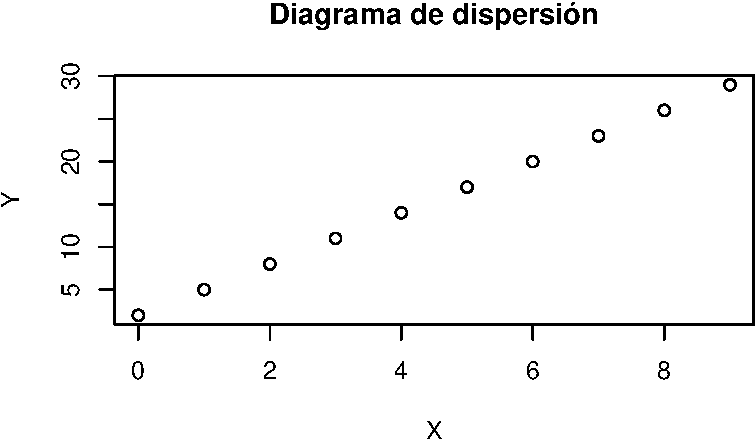
\includegraphics[keepaspectratio]{06-regresion_files/figure-pdf/unnamed-chunk-2-1.pdf}}

  \end{tcolorbox}

  \begin{tcolorbox}[enhanced jigsaw, breakable, toptitle=1mm, colbacktitle=quarto-callout-tip-color!10!white, rightrule=.15mm, opacityback=0, opacitybacktitle=0.6, titlerule=0mm, coltitle=black, colframe=quarto-callout-tip-color-frame, colback=white, bottomtitle=1mm, leftrule=.75mm, toprule=.15mm, title=\textcolor{quarto-callout-tip-color}{\faLightbulb}\hspace{0.5em}{Solución 2}, arc=.35mm, bottomrule=.15mm, left=2mm]

  Otra alternativa es usar la función la función
  \href{https://aprendeconalf.es/manual-r/07-graficos.html\#diagramas-de-puntos}{\texttt{geom\_point}}
  del paquete \texttt{ggplot2}.

\begin{Shaded}
\begin{Highlighting}[]
\FunctionTok{library}\NormalTok{(ggplot2)}
\FunctionTok{ggplot}\NormalTok{(df, }\FunctionTok{aes}\NormalTok{(}\AttributeTok{x =}\NormalTok{ x, }\AttributeTok{y =}\NormalTok{ y)) }\SpecialCharTok{+}
    \FunctionTok{geom\_point}\NormalTok{(}\AttributeTok{col =} \StringTok{"red"}\NormalTok{) }\SpecialCharTok{+}
    \FunctionTok{labs}\NormalTok{(}\AttributeTok{title =} \StringTok{"Diagrama de dispersión"}\NormalTok{, }\AttributeTok{x =} \StringTok{"X"}\NormalTok{, }\AttributeTok{y =} \StringTok{"Y"}\NormalTok{)}
\end{Highlighting}
\end{Shaded}

  \pandocbounded{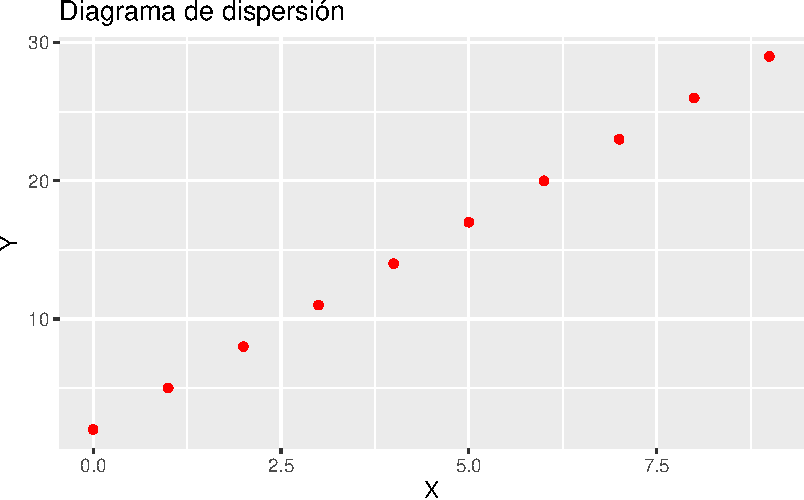
\includegraphics[keepaspectratio]{06-regresion_files/figure-pdf/unnamed-chunk-3-1.pdf}}

  El tipo de modelo que mejor se ajusta es lineal, ya que todos los
  puntos están alineados.

  \end{tcolorbox}
\item
  Calcular la recta de regresión de \(Y\) sobre \(X\).

  \begin{tcolorbox}[enhanced jigsaw, breakable, toptitle=1mm, colbacktitle=quarto-callout-tip-color!10!white, rightrule=.15mm, opacityback=0, opacitybacktitle=0.6, titlerule=0mm, coltitle=black, colframe=quarto-callout-tip-color-frame, colback=white, bottomtitle=1mm, leftrule=.75mm, toprule=.15mm, title=\textcolor{quarto-callout-tip-color}{\faLightbulb}\hspace{0.5em}{Solución}, arc=.35mm, bottomrule=.15mm, left=2mm]

  Para ajustar un modelo de regresión se utiliza la función
  \href{https://www.rdocumentation.org/packages/stats/versions/3.6.2/topics/lm}{\texttt{lm}}
  del paquete \texttt{stats}. Esta función requiere que se le pase como
  parámetro la fórmula del modelo de regresión que debe tener la
  sintaxis \texttt{y\ \textasciitilde{}\ f(x)}, donde \texttt{y} es la
  variable dependiente en el modelo, \texttt{x} es la variable
  independiente, y \texttt{f(x)} es una expresión matemática que
  describe el modelo.

\begin{Shaded}
\begin{Highlighting}[]
\NormalTok{recta\_y\_x }\OtherTok{\textless{}{-}} \FunctionTok{lm}\NormalTok{(y }\SpecialCharTok{\textasciitilde{}}\NormalTok{ x, df) }
\FunctionTok{summary}\NormalTok{(recta\_y\_x)}
\end{Highlighting}
\end{Shaded}

\begin{verbatim}

Call:
lm(formula = y ~ x, data = df)

Residuals:
       Min         1Q     Median         3Q        Max 
-3.675e-15 -8.783e-16  5.168e-16  9.646e-16  1.944e-15 

Coefficients:
             Estimate Std. Error   t value Pr(>|t|)    
(Intercept) 2.000e+00  1.049e-15 1.906e+15   <2e-16 ***
x           3.000e+00  1.965e-16 1.527e+16   <2e-16 ***
---
Signif. codes:  0 '***' 0.001 '**' 0.01 '*' 0.05 '.' 0.1 ' ' 1

Residual standard error: 1.785e-15 on 8 degrees of freedom
Multiple R-squared:      1, Adjusted R-squared:      1 
F-statistic: 2.33e+32 on 1 and 8 DF,  p-value: < 2.2e-16
\end{verbatim}

  La recta de regresión de \(Y\) sobre \(X\) es \(y = 2 + 3 x\).

  \end{tcolorbox}
\item
  Obtener el coeficiente de regresión de la recta anterior e
  interpretarlo.

  \begin{tcolorbox}[enhanced jigsaw, breakable, toptitle=1mm, colbacktitle=quarto-callout-tip-color!10!white, rightrule=.15mm, opacityback=0, opacitybacktitle=0.6, titlerule=0mm, coltitle=black, colframe=quarto-callout-tip-color-frame, colback=white, bottomtitle=1mm, leftrule=.75mm, toprule=.15mm, title=\textcolor{quarto-callout-tip-color}{\faLightbulb}\hspace{0.5em}{Solución}, arc=.35mm, bottomrule=.15mm, left=2mm]

  El coeficiente de regresión es la pendiente de la recta de regresión

\begin{Shaded}
\begin{Highlighting}[]
\FunctionTok{cat}\NormalTok{(}\FunctionTok{paste}\NormalTok{(}\StringTok{"Coeficiente de regresión de Y sobre X:"}\NormalTok{, recta\_y\_x}\SpecialCharTok{$}\NormalTok{coefficients[[}\StringTok{"x"}\NormalTok{]]))}
\end{Highlighting}
\end{Shaded}

\begin{verbatim}
Coeficiente de regresión de Y sobre X: 3
\end{verbatim}

  El coeficiente de regresión de \(Y\) sobre \(X\) vale 3, lo que indica
  que \(Y\) aumenta 3 unidades por cada unidad que aumenta \(X\).

  \end{tcolorbox}
\item
  Dibujar la recta de regresión de \(Y\) sobre \(X\) sobre el diagrama
  de dispersión. ¿Cómo son los residuos del modelo de regresión?

  \begin{tcolorbox}[enhanced jigsaw, breakable, toptitle=1mm, colbacktitle=quarto-callout-tip-color!10!white, rightrule=.15mm, opacityback=0, opacitybacktitle=0.6, titlerule=0mm, coltitle=black, colframe=quarto-callout-tip-color-frame, colback=white, bottomtitle=1mm, leftrule=.75mm, toprule=.15mm, title=\textcolor{quarto-callout-tip-color}{\faLightbulb}\hspace{0.5em}{Solución 1}, arc=.35mm, bottomrule=.15mm, left=2mm]

  Para dibujar la recta de regresión se puede usar la función
  \href{https://www.rdocumentation.org/packages/graphics/versions/3.6.2/topics/abline}{\texttt{abline}}
  del paquete \texttt{graphics}.

\begin{Shaded}
\begin{Highlighting}[]
\FunctionTok{plot}\NormalTok{(df}\SpecialCharTok{$}\NormalTok{x, df}\SpecialCharTok{$}\NormalTok{y, }\AttributeTok{xlab =} \StringTok{"X"}\NormalTok{, }\AttributeTok{ylab =} \StringTok{"Y"}\NormalTok{, }\AttributeTok{main =} \StringTok{"Diagrama de dispersión"}\NormalTok{)}
\FunctionTok{abline}\NormalTok{(recta\_y\_x)}
\end{Highlighting}
\end{Shaded}

  \pandocbounded{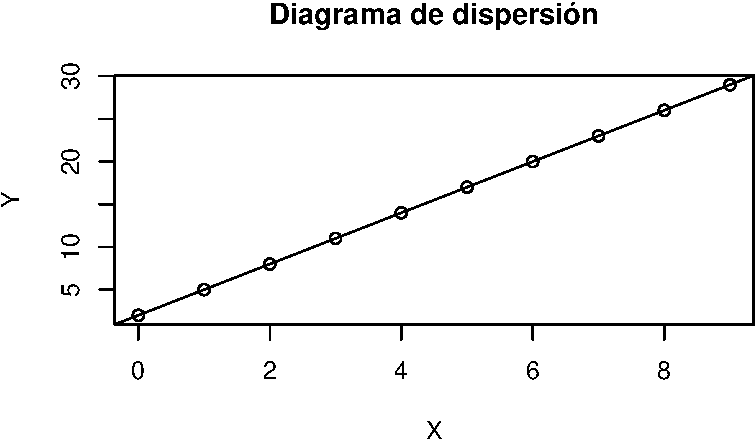
\includegraphics[keepaspectratio]{06-regresion_files/figure-pdf/unnamed-chunk-6-1.pdf}}

  \end{tcolorbox}

  \begin{tcolorbox}[enhanced jigsaw, breakable, toptitle=1mm, colbacktitle=quarto-callout-tip-color!10!white, rightrule=.15mm, opacityback=0, opacitybacktitle=0.6, titlerule=0mm, coltitle=black, colframe=quarto-callout-tip-color-frame, colback=white, bottomtitle=1mm, leftrule=.75mm, toprule=.15mm, title=\textcolor{quarto-callout-tip-color}{\faLightbulb}\hspace{0.5em}{Solución 2}, arc=.35mm, bottomrule=.15mm, left=2mm]

  Otra alternativa es usar la geometría de ajuste de regresión por
  mínimos cuadrados
  \href{https://aprendeconalf.es/manual-r/07-graficos.html\#interpolaci\%C3\%B3n-y-ajustes-de-regresi\%C3\%B3n}{\texttt{geom\_smooth}}
  del paquete \texttt{ggplot2}.

\begin{Shaded}
\begin{Highlighting}[]
\FunctionTok{library}\NormalTok{(ggplot2)}
\FunctionTok{ggplot}\NormalTok{(df, }\FunctionTok{aes}\NormalTok{(}\AttributeTok{x =}\NormalTok{ x, }\AttributeTok{y =}\NormalTok{ y)) }\SpecialCharTok{+}
    \FunctionTok{geom\_point}\NormalTok{(}\AttributeTok{col =} \StringTok{"red"}\NormalTok{) }\SpecialCharTok{+}
    \FunctionTok{geom\_smooth}\NormalTok{(}\AttributeTok{method =} \StringTok{"lm"}\NormalTok{) }\SpecialCharTok{+}
    \FunctionTok{labs}\NormalTok{(}\AttributeTok{title =} \StringTok{"Diagrama de dispersión"}\NormalTok{, }\AttributeTok{x =} \StringTok{"X"}\NormalTok{, }\AttributeTok{y =} \StringTok{"Y"}\NormalTok{)}
\end{Highlighting}
\end{Shaded}

  \pandocbounded{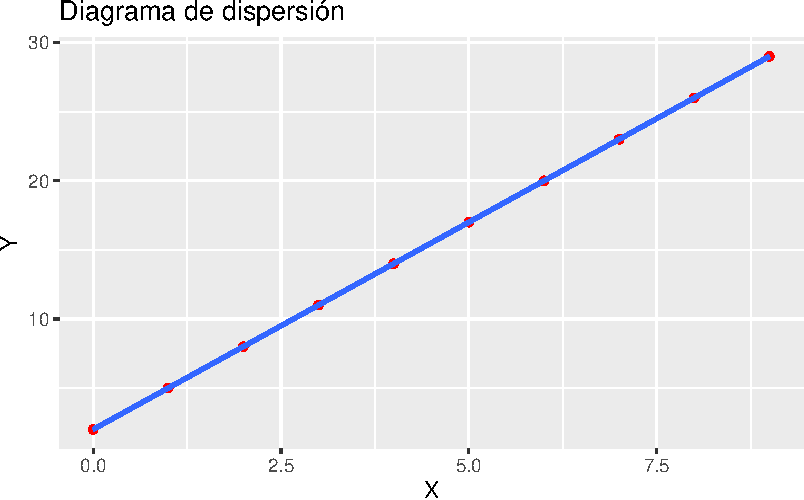
\includegraphics[keepaspectratio]{06-regresion_files/figure-pdf/unnamed-chunk-7-1.pdf}}

  Como la recta pasa por todos los puntos del diagrama de dispersión,
  los residuos son nulos.

  \end{tcolorbox}
\item
  Calcular el coeficiente de determinación del modelo lineal e
  interpretarlo.

  \begin{tcolorbox}[enhanced jigsaw, breakable, toptitle=1mm, colbacktitle=quarto-callout-tip-color!10!white, rightrule=.15mm, opacityback=0, opacitybacktitle=0.6, titlerule=0mm, coltitle=black, colframe=quarto-callout-tip-color-frame, colback=white, bottomtitle=1mm, leftrule=.75mm, toprule=.15mm, title=\textcolor{quarto-callout-tip-color}{\faLightbulb}\hspace{0.5em}{Solución}, arc=.35mm, bottomrule=.15mm, left=2mm]

\begin{Shaded}
\begin{Highlighting}[]
\FunctionTok{cat}\NormalTok{(}\FunctionTok{paste}\NormalTok{(}\StringTok{"Coeficiente de determinación lineal R²:"}\NormalTok{, }\FunctionTok{summary}\NormalTok{(recta\_y\_x)}\SpecialCharTok{$}\NormalTok{r.squared))}
\end{Highlighting}
\end{Shaded}

\begin{verbatim}
Coeficiente de determinación lineal R²: 1
\end{verbatim}

  Como el coeficiente de determinación lineal vale 1, el ajuste de la
  recta de regresión es perfecto.

  \end{tcolorbox}
\item
  Calcular la recta de regresión de \(X\) sobre \(Y\). ¿Coincide con la
  recta de regresión de \(Y\) sobre \(X\)?

  \begin{tcolorbox}[enhanced jigsaw, breakable, toptitle=1mm, colbacktitle=quarto-callout-tip-color!10!white, rightrule=.15mm, opacityback=0, opacitybacktitle=0.6, titlerule=0mm, coltitle=black, colframe=quarto-callout-tip-color-frame, colback=white, bottomtitle=1mm, leftrule=.75mm, toprule=.15mm, title=\textcolor{quarto-callout-tip-color}{\faLightbulb}\hspace{0.5em}{Solución}, arc=.35mm, bottomrule=.15mm, left=2mm]

\begin{Shaded}
\begin{Highlighting}[]
\NormalTok{recta\_x\_y }\OtherTok{\textless{}{-}} \FunctionTok{lm}\NormalTok{(x }\SpecialCharTok{\textasciitilde{}}\NormalTok{ y, df) }
\FunctionTok{summary}\NormalTok{(recta\_x\_y)}
\end{Highlighting}
\end{Shaded}

\begin{verbatim}

Call:
lm(formula = x ~ y, data = df)

Residuals:
       Min         1Q     Median         3Q        Max 
-8.668e-16 -4.345e-16 -8.827e-17  3.905e-16  1.196e-15 

Coefficients:
              Estimate Std. Error    t value Pr(>|t|)    
(Intercept) -6.667e-01  4.215e-16 -1.582e+15   <2e-16 ***
y            3.333e-01  2.377e-17  1.402e+16   <2e-16 ***
---
Signif. codes:  0 '***' 0.001 '**' 0.01 '*' 0.05 '.' 0.1 ' ' 1

Residual standard error: 6.477e-16 on 8 degrees of freedom
Multiple R-squared:      1, Adjusted R-squared:      1 
F-statistic: 1.967e+32 on 1 and 8 DF,  p-value: < 2.2e-16
\end{verbatim}

  La recta de regresión de \(X\) sobre \(Y\) es
  \(x = -0.6666667 + 0.3333333 x\), que es la misma que la recta de
  \(Y\) sobre \(X\), ya que el ajuste es perfecto, y tanto los residuos
  en \(Y\) como los residuos en \(X\) valen cero para esta recta.

  \end{tcolorbox}
\end{enumerate}

\end{exercise}

\begin{exercise}[]\protect\hypertarget{exr-regresion-2}{}\label{exr-regresion-2}

El fichero \href{datos/horas-estudio.csv}{\texttt{horas-estudio.csv}}
contiene información sobre las horas de estudio diarias de una muestra
de alumnos de ingeniería, y el número de asignaturas suspendidas al
final del curso.

\begin{enumerate}
\def\labelenumi{\alph{enumi}.}
\item
  Crear un data frame con los datos de las horas de estudio y los
  suspensos a partir del fichero
  \href{https://aprendeconalf.es/estadistica-practicas-r/datos/horas-estudio.csv}{\texttt{horas-estudio.csv}}.

  \begin{tcolorbox}[enhanced jigsaw, breakable, toptitle=1mm, colbacktitle=quarto-callout-tip-color!10!white, rightrule=.15mm, opacityback=0, opacitybacktitle=0.6, titlerule=0mm, coltitle=black, colframe=quarto-callout-tip-color-frame, colback=white, bottomtitle=1mm, leftrule=.75mm, toprule=.15mm, title=\textcolor{quarto-callout-tip-color}{\faLightbulb}\hspace{0.5em}{Solución}, arc=.35mm, bottomrule=.15mm, left=2mm]

\begin{Shaded}
\begin{Highlighting}[]
\FunctionTok{library}\NormalTok{(readr)}
\NormalTok{df }\OtherTok{\textless{}{-}} \FunctionTok{read\_csv}\NormalTok{(}\StringTok{"https://aprendeconalf.es/estadistica{-}practicas{-}r/datos/horas{-}estudio.csv"}\NormalTok{)}
\NormalTok{df}
\end{Highlighting}
\end{Shaded}

\begin{verbatim}
# A tibble: 30 x 2
   Horas Suspensos
   <dbl>     <dbl>
 1   3.5         1
 2   0.6         5
 3   2.8         1
 4   2.5         3
 5   2.6         1
 6   3.9         0
 7   1.5         3
 8   0.7         3
 9   3.6         1
10   3.7         1
# i 20 more rows
\end{verbatim}

  \end{tcolorbox}
\item
  Dibujar el diagrama de dispersión correspondiente. ¿Qué tipo de modelo
  de regresión se ajusta mejor a la nube de puntos?

  \begin{tcolorbox}[enhanced jigsaw, breakable, toptitle=1mm, colbacktitle=quarto-callout-tip-color!10!white, rightrule=.15mm, opacityback=0, opacitybacktitle=0.6, titlerule=0mm, coltitle=black, colframe=quarto-callout-tip-color-frame, colback=white, bottomtitle=1mm, leftrule=.75mm, toprule=.15mm, title=\textcolor{quarto-callout-tip-color}{\faLightbulb}\hspace{0.5em}{Solución}, arc=.35mm, bottomrule=.15mm, left=2mm]

\begin{Shaded}
\begin{Highlighting}[]
\FunctionTok{library}\NormalTok{(ggplot2)}
\FunctionTok{ggplot}\NormalTok{(df, }\FunctionTok{aes}\NormalTok{(}\AttributeTok{x =}\NormalTok{ Horas, }\AttributeTok{y =}\NormalTok{ Suspensos)) }\SpecialCharTok{+}
    \FunctionTok{geom\_point}\NormalTok{(}\AttributeTok{col =} \StringTok{"red"}\NormalTok{) }\SpecialCharTok{+}
    \FunctionTok{labs}\NormalTok{(}\AttributeTok{title =} \StringTok{"Diagrama de dispersión"}\NormalTok{, }\AttributeTok{x =} \StringTok{"Horas de estudio"}\NormalTok{, }\AttributeTok{y =} \StringTok{"Asignaturas suspensas"}\NormalTok{)}
\end{Highlighting}
\end{Shaded}

  \pandocbounded{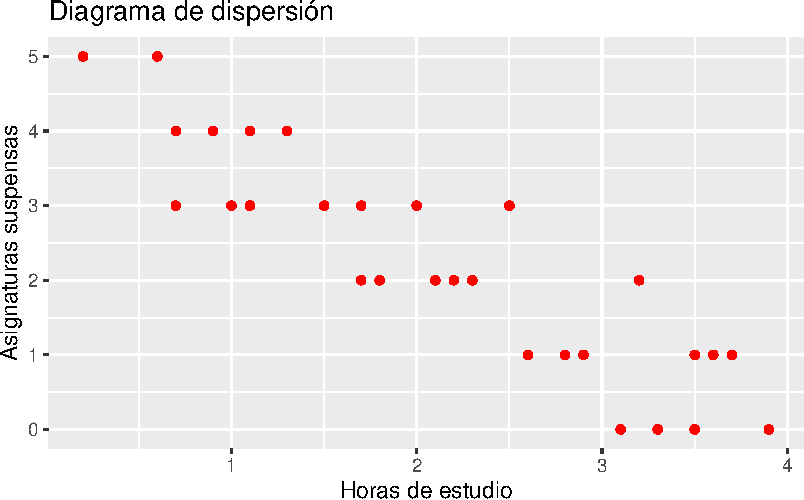
\includegraphics[keepaspectratio]{06-regresion_files/figure-pdf/unnamed-chunk-11-1.pdf}}

  El tipo de modelo que mejor se ajusta es lineal, ya que hay una
  tendencia lineal en la nube de puntos y además es inversa.

  \end{tcolorbox}
\item
  Calcular la recta de regresión de los suspensos sobre las horas de
  estudio.

  \begin{tcolorbox}[enhanced jigsaw, breakable, toptitle=1mm, colbacktitle=quarto-callout-tip-color!10!white, rightrule=.15mm, opacityback=0, opacitybacktitle=0.6, titlerule=0mm, coltitle=black, colframe=quarto-callout-tip-color-frame, colback=white, bottomtitle=1mm, leftrule=.75mm, toprule=.15mm, title=\textcolor{quarto-callout-tip-color}{\faLightbulb}\hspace{0.5em}{Solución}, arc=.35mm, bottomrule=.15mm, left=2mm]

\begin{Shaded}
\begin{Highlighting}[]
\NormalTok{recta\_suspensos\_horas }\OtherTok{\textless{}{-}} \FunctionTok{lm}\NormalTok{(Suspensos }\SpecialCharTok{\textasciitilde{}}\NormalTok{ Horas, df) }
\FunctionTok{summary}\NormalTok{(recta\_suspensos\_horas)}
\end{Highlighting}
\end{Shaded}

\begin{verbatim}

Call:
lm(formula = Suspensos ~ Horas, data = df)

Residuals:
     Min       1Q   Median       3Q      Max 
-1.03614 -0.53214 -0.02013  0.49187  1.22587 

Coefficients:
            Estimate Std. Error t value Pr(>|t|)    
(Intercept)   4.8491     0.2622   18.49  < 2e-16 ***
Horas        -1.2300     0.1106  -11.12  8.7e-12 ***
---
Signif. codes:  0 '***' 0.001 '**' 0.01 '*' 0.05 '.' 0.1 ' ' 1

Residual standard error: 0.6359 on 28 degrees of freedom
Multiple R-squared:  0.8155,    Adjusted R-squared:  0.8089 
F-statistic: 123.8 on 1 and 28 DF,  p-value: 8.7e-12
\end{verbatim}

  La recta de regresión de los suspensos sobre las horas es
  \(\textsf{suspensos}= 4.8491273 + -1.2299972 \textsf{horas}\).

  \end{tcolorbox}
\item
  Obtener el coeficiente de regresión de la recta anterior e
  interpretarlo.

  \begin{tcolorbox}[enhanced jigsaw, breakable, toptitle=1mm, colbacktitle=quarto-callout-tip-color!10!white, rightrule=.15mm, opacityback=0, opacitybacktitle=0.6, titlerule=0mm, coltitle=black, colframe=quarto-callout-tip-color-frame, colback=white, bottomtitle=1mm, leftrule=.75mm, toprule=.15mm, title=\textcolor{quarto-callout-tip-color}{\faLightbulb}\hspace{0.5em}{Solución}, arc=.35mm, bottomrule=.15mm, left=2mm]

\begin{Shaded}
\begin{Highlighting}[]
\FunctionTok{cat}\NormalTok{(}\FunctionTok{paste}\NormalTok{(}\StringTok{"Coeficiente de regresión de Suspensos sobre Horas:"}\NormalTok{, recta\_suspensos\_horas}\SpecialCharTok{$}\NormalTok{coefficients[[}\StringTok{"Horas"}\NormalTok{]]))}
\end{Highlighting}
\end{Shaded}

\begin{verbatim}
Coeficiente de regresión de Suspensos sobre Horas: -1.22999717844331
\end{verbatim}

  El coeficiente de regresión de los suspensos sobre las horas de
  estudio vale -1.2299972, lo que indica que por cada hora de estudio se
  obtendrán 1.2299972 suspensos menos al final del curso.

  \end{tcolorbox}
\item
  Dibujar la recta de regresión sobre el diagrama de dispersión. ¿El
  ajuste es mejor o peor que el del ejercicio anterior?

  \begin{tcolorbox}[enhanced jigsaw, breakable, toptitle=1mm, colbacktitle=quarto-callout-tip-color!10!white, rightrule=.15mm, opacityback=0, opacitybacktitle=0.6, titlerule=0mm, coltitle=black, colframe=quarto-callout-tip-color-frame, colback=white, bottomtitle=1mm, leftrule=.75mm, toprule=.15mm, title=\textcolor{quarto-callout-tip-color}{\faLightbulb}\hspace{0.5em}{Solución}, arc=.35mm, bottomrule=.15mm, left=2mm]

\begin{Shaded}
\begin{Highlighting}[]
\FunctionTok{library}\NormalTok{(ggplot2)}
\FunctionTok{ggplot}\NormalTok{(df, }\FunctionTok{aes}\NormalTok{(}\AttributeTok{x =}\NormalTok{ Horas, }\AttributeTok{y =}\NormalTok{ Suspensos)) }\SpecialCharTok{+}
    \FunctionTok{geom\_point}\NormalTok{(}\AttributeTok{col =} \StringTok{"red"}\NormalTok{) }\SpecialCharTok{+}
    \FunctionTok{geom\_smooth}\NormalTok{(}\AttributeTok{method =} \StringTok{"lm"}\NormalTok{) }\SpecialCharTok{+}
    \FunctionTok{labs}\NormalTok{(}\AttributeTok{title =} \StringTok{"Diagrama de dispersión"}\NormalTok{, }\AttributeTok{x =} \StringTok{"Horas de estudio"}\NormalTok{, }\AttributeTok{y =} \StringTok{"Asignaturas suspensas"}\NormalTok{)}
\end{Highlighting}
\end{Shaded}

  \pandocbounded{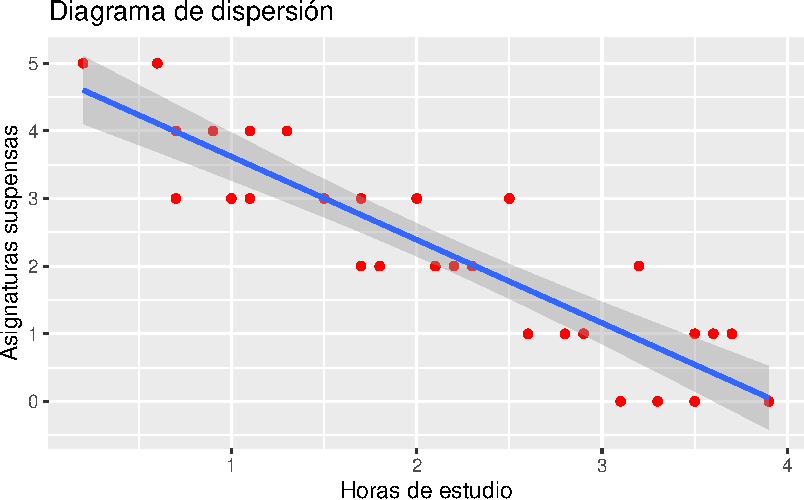
\includegraphics[keepaspectratio]{06-regresion_files/figure-pdf/unnamed-chunk-14-1.pdf}}

  En este caso el ajuste no es perfecto, ya que es imposible que la
  recta pase por todos los puntos como ocurría en el ejercicio anterior.
  Por tanto, el ajuste es peor.

  \end{tcolorbox}
\item
  Calcular el coeficiente de determinación del modelo lineal e
  interpretarlo.

  \begin{tcolorbox}[enhanced jigsaw, breakable, toptitle=1mm, colbacktitle=quarto-callout-tip-color!10!white, rightrule=.15mm, opacityback=0, opacitybacktitle=0.6, titlerule=0mm, coltitle=black, colframe=quarto-callout-tip-color-frame, colback=white, bottomtitle=1mm, leftrule=.75mm, toprule=.15mm, title=\textcolor{quarto-callout-tip-color}{\faLightbulb}\hspace{0.5em}{Solución}, arc=.35mm, bottomrule=.15mm, left=2mm]

\begin{Shaded}
\begin{Highlighting}[]
\FunctionTok{cat}\NormalTok{(}\FunctionTok{paste}\NormalTok{(}\StringTok{"Coeficiente de determinación lineal R²:"}\NormalTok{, }\FunctionTok{summary}\NormalTok{(recta\_suspensos\_horas)}\SpecialCharTok{$}\NormalTok{r.squared))}
\end{Highlighting}
\end{Shaded}

\begin{verbatim}
Coeficiente de determinación lineal R²: 0.81549948723949
\end{verbatim}

  Como el coeficiente de determinación lineal vale 0.8154995 que está
  bastante próximo a 1, el ajuste es bueno, y el modelo puede utilizarse
  con fines predictivos.

  \end{tcolorbox}
\item
  Utilizar la recta de regresión para predecir el número de suspensos
  correspondiente a 3 horas de estudio diarias. ¿Es fiable esta
  predicción?

  \begin{tcolorbox}[enhanced jigsaw, breakable, toptitle=1mm, colbacktitle=quarto-callout-tip-color!10!white, rightrule=.15mm, opacityback=0, opacitybacktitle=0.6, titlerule=0mm, coltitle=black, colframe=quarto-callout-tip-color-frame, colback=white, bottomtitle=1mm, leftrule=.75mm, toprule=.15mm, title=\textcolor{quarto-callout-tip-color}{\faLightbulb}\hspace{0.5em}{Solución}, arc=.35mm, bottomrule=.15mm, left=2mm]

\begin{Shaded}
\begin{Highlighting}[]
\FunctionTok{predict.lm}\NormalTok{(recta\_suspensos\_horas, }\AttributeTok{newdata =} \FunctionTok{list}\NormalTok{(}\AttributeTok{Horas =} \DecValTok{3}\NormalTok{))}
\end{Highlighting}
\end{Shaded}

\begin{verbatim}
       1 
1.159136 
\end{verbatim}

  La predicción será fiable ya que el coeficiente de determinación está
  próximo a 1 y el tamaño de la muestra no es muy pequeño.

  \end{tcolorbox}
\item
  Según el modelo lineal, ¿cuántas horas diarias tendrá que estudiar
  como mínimo un alumno si quiere aprobarlo todo?

  \begin{tcolorbox}[enhanced jigsaw, breakable, toptitle=1mm, colbacktitle=quarto-callout-tip-color!10!white, rightrule=.15mm, opacityback=0, opacitybacktitle=0.6, titlerule=0mm, coltitle=black, colframe=quarto-callout-tip-color-frame, colback=white, bottomtitle=1mm, leftrule=.75mm, toprule=.15mm, title=\textcolor{quarto-callout-tip-color}{\faLightbulb}\hspace{0.5em}{Solución}, arc=.35mm, bottomrule=.15mm, left=2mm]

  Como ahora queremos predecir el número de horas de estudio,
  necesitamos calcular la recta de regresión de la horas sobre los
  suspensos.

\begin{Shaded}
\begin{Highlighting}[]
\NormalTok{recta\_horas\_suspensos }\OtherTok{\textless{}{-}} \FunctionTok{lm}\NormalTok{(Horas }\SpecialCharTok{\textasciitilde{}}\NormalTok{ Suspensos, df) }
\FunctionTok{predict.lm}\NormalTok{(recta\_horas\_suspensos, }\AttributeTok{newdata =} \FunctionTok{list}\NormalTok{(}\AttributeTok{Suspensos =} \DecValTok{0}\NormalTok{))}
\end{Highlighting}
\end{Shaded}

\begin{verbatim}
       1 
3.607387 
\end{verbatim}

  \end{tcolorbox}
\end{enumerate}

\end{exercise}

\begin{exercise}[]\protect\hypertarget{exr-regresion-3}{}\label{exr-regresion-3}

Después de tomar un litro de vino se ha medido la concentración de
alcohol en la sangre en distintos instantes, obteniendo los siguientes
datos

\[
\begin{array}{lrrrrrrr}
\hline 
\mbox{Tiempo después (minutos)} & 30 & 60 & 90 & 120 & 150 & 180 & 210\\ 
\mbox{Alcohol (gramos/litro)} & 1.6 & 1.7 & 1.5 & 1.1 & 0.7 & 0.2 & 2.1\\
\hline
\end{array}
\]

\begin{enumerate}
\def\labelenumi{\alph{enumi}.}
\item
  Crear un data frame con los datos del tiempo y la concentración de
  alcohol.

  \begin{tcolorbox}[enhanced jigsaw, breakable, toptitle=1mm, colbacktitle=quarto-callout-tip-color!10!white, rightrule=.15mm, opacityback=0, opacitybacktitle=0.6, titlerule=0mm, coltitle=black, colframe=quarto-callout-tip-color-frame, colback=white, bottomtitle=1mm, leftrule=.75mm, toprule=.15mm, title=\textcolor{quarto-callout-tip-color}{\faLightbulb}\hspace{0.5em}{Solución}, arc=.35mm, bottomrule=.15mm, left=2mm]

\begin{Shaded}
\begin{Highlighting}[]
\NormalTok{df }\OtherTok{\textless{}{-}} \FunctionTok{data.frame}\NormalTok{(}
    \AttributeTok{Tiempo =} \FunctionTok{c}\NormalTok{(}\DecValTok{30}\NormalTok{, }\DecValTok{60}\NormalTok{, }\DecValTok{90}\NormalTok{, }\DecValTok{120}\NormalTok{, }\DecValTok{150}\NormalTok{, }\DecValTok{180}\NormalTok{, }\DecValTok{210}\NormalTok{),}
    \AttributeTok{Alcohol =} \FunctionTok{c}\NormalTok{(}\FloatTok{1.6}\NormalTok{, }\FloatTok{1.7}\NormalTok{, }\FloatTok{1.5}\NormalTok{, }\FloatTok{1.1}\NormalTok{, }\FloatTok{0.7}\NormalTok{, }\FloatTok{0.2}\NormalTok{, }\FloatTok{2.1}\NormalTok{)}
\NormalTok{)}
\NormalTok{df}
\end{Highlighting}
\end{Shaded}

\begin{verbatim}
  Tiempo Alcohol
1     30     1.6
2     60     1.7
3     90     1.5
4    120     1.1
5    150     0.7
6    180     0.2
7    210     2.1
\end{verbatim}

  \end{tcolorbox}
\item
  Calcular el coeficiente de correlación lineal. ¿Existe relación lineal
  entre la concentración de alcohol y el tiempo que pasa?

  \begin{tcolorbox}[enhanced jigsaw, breakable, toptitle=1mm, colbacktitle=quarto-callout-tip-color!10!white, rightrule=.15mm, opacityback=0, opacitybacktitle=0.6, titlerule=0mm, coltitle=black, colframe=quarto-callout-tip-color-frame, colback=white, bottomtitle=1mm, leftrule=.75mm, toprule=.15mm, title=\textcolor{quarto-callout-tip-color}{\faLightbulb}\hspace{0.5em}{Solución}, arc=.35mm, bottomrule=.15mm, left=2mm]

  Para calcular el coeficiente de correlación lineal de Pearson se puede
  utilar la función
  \href{https://www.rdocumentation.org/packages/stats/versions/3.6.2/topics/cor}{\texttt{cor}}
  del paquete \texttt{stats}.

\begin{Shaded}
\begin{Highlighting}[]
\FunctionTok{cor}\NormalTok{(df}\SpecialCharTok{$}\NormalTok{Tiempo, df}\SpecialCharTok{$}\NormalTok{Alcohol)}
\end{Highlighting}
\end{Shaded}

\begin{verbatim}
[1] -0.2730367
\end{verbatim}

  El valore del coeficiente de correlación lineal es muy bajo, por lo
  que aparentemente no hay relación lineal entre la concentración de
  alcohol en sangre y el tiempo que pasa.

  \end{tcolorbox}
\item
  Dibujar el diagrama de dispersión correspondiente y la recta de
  regresión de la concentración de alcohol sobre el tiempo. ¿Por qué el
  ajuste es tan malo?

  \begin{tcolorbox}[enhanced jigsaw, breakable, toptitle=1mm, colbacktitle=quarto-callout-tip-color!10!white, rightrule=.15mm, opacityback=0, opacitybacktitle=0.6, titlerule=0mm, coltitle=black, colframe=quarto-callout-tip-color-frame, colback=white, bottomtitle=1mm, leftrule=.75mm, toprule=.15mm, title=\textcolor{quarto-callout-tip-color}{\faLightbulb}\hspace{0.5em}{Solución}, arc=.35mm, bottomrule=.15mm, left=2mm]

\begin{Shaded}
\begin{Highlighting}[]
\FunctionTok{library}\NormalTok{(ggplot2)}
\FunctionTok{ggplot}\NormalTok{(df, }\FunctionTok{aes}\NormalTok{(}\AttributeTok{x =}\NormalTok{ Tiempo, }\AttributeTok{y =}\NormalTok{ Alcohol)) }\SpecialCharTok{+}
    \FunctionTok{geom\_point}\NormalTok{(}\AttributeTok{col =} \StringTok{"red"}\NormalTok{) }\SpecialCharTok{+}
    \FunctionTok{geom\_smooth}\NormalTok{(}\AttributeTok{method =} \StringTok{"lm"}\NormalTok{) }\SpecialCharTok{+}
    \FunctionTok{labs}\NormalTok{(}\AttributeTok{title =} \StringTok{"Diagrama de dispersión"}\NormalTok{, }\AttributeTok{x =} \StringTok{"Tiempo en minutos"}\NormalTok{, }\AttributeTok{y =} \StringTok{"Concentración de alcohol en sangre (g/l)"}\NormalTok{)}
\end{Highlighting}
\end{Shaded}

  \pandocbounded{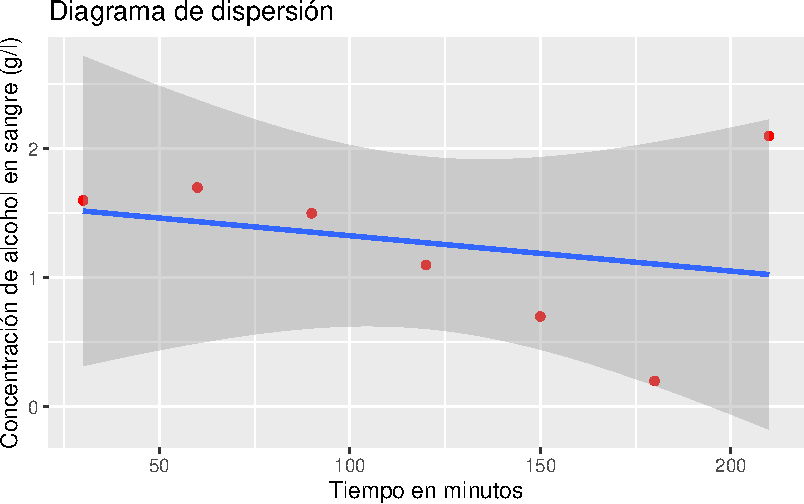
\includegraphics[keepaspectratio]{06-regresion_files/figure-pdf/unnamed-chunk-20-1.pdf}}

  El ajuste es malo porque hay un dato atípico que no sigue la misma
  tendencia que el resto.

  \end{tcolorbox}
\item
  Eliminar el dato atípico y calcular la recta de la concentración de
  alcohol sobre el tiempo. ¿Ha mejorado el modelo?

  \begin{tcolorbox}[enhanced jigsaw, breakable, toptitle=1mm, colbacktitle=quarto-callout-tip-color!10!white, rightrule=.15mm, opacityback=0, opacitybacktitle=0.6, titlerule=0mm, coltitle=black, colframe=quarto-callout-tip-color-frame, colback=white, bottomtitle=1mm, leftrule=.75mm, toprule=.15mm, title=\textcolor{quarto-callout-tip-color}{\faLightbulb}\hspace{0.5em}{Solución}, arc=.35mm, bottomrule=.15mm, left=2mm]

\begin{Shaded}
\begin{Highlighting}[]
\CommentTok{\# Eliminamos el dato atípico que está en la fila }
\NormalTok{df }\OtherTok{\textless{}{-}}\NormalTok{ df[}\SpecialCharTok{{-}}\FunctionTok{c}\NormalTok{(}\DecValTok{7}\NormalTok{), ]}
\NormalTok{recta\_alcohol\_tiempo }\OtherTok{\textless{}{-}} \FunctionTok{lm}\NormalTok{(Alcohol }\SpecialCharTok{\textasciitilde{}}\NormalTok{ Tiempo, df) }
\FunctionTok{summary}\NormalTok{(recta\_alcohol\_tiempo)}
\end{Highlighting}
\end{Shaded}

\begin{verbatim}

Call:
lm(formula = Alcohol ~ Tiempo, data = df)

Residuals:
       1        2        3        4        5        6 
-0.27619  0.12095  0.21810  0.11524  0.01238 -0.19048 

Coefficients:
             Estimate Std. Error t value Pr(>|t|)    
(Intercept)  2.173333   0.201927  10.763 0.000423 ***
Tiempo      -0.009905   0.001728  -5.731 0.004591 ** 
---
Signif. codes:  0 '***' 0.001 '**' 0.01 '*' 0.05 '.' 0.1 ' ' 1

Residual standard error: 0.2169 on 4 degrees of freedom
Multiple R-squared:  0.8914,    Adjusted R-squared:  0.8643 
F-statistic: 32.84 on 1 and 4 DF,  p-value: 0.004591
\end{verbatim}

  La recta de regresión de la concentración de alcohol en sangre sobre
  el tiempo es
  \(\textsf{alcohol}= 2.1733333 + -0.0099048 \textsf{tiempo}\).

  El modelo ha mejorado notablemente ya que ahora el coeficiente de
  determinación lineal \(R^2=0.8914286\), que está muy próximo a 1.

  \end{tcolorbox}
\item
  Según el modelo de regresión lineal, ¿a qué velocidad metaboliza esta
  persona el alcohol?

  \begin{tcolorbox}[enhanced jigsaw, breakable, toptitle=1mm, colbacktitle=quarto-callout-tip-color!10!white, rightrule=.15mm, opacityback=0, opacitybacktitle=0.6, titlerule=0mm, coltitle=black, colframe=quarto-callout-tip-color-frame, colback=white, bottomtitle=1mm, leftrule=.75mm, toprule=.15mm, title=\textcolor{quarto-callout-tip-color}{\faLightbulb}\hspace{0.5em}{Solución}, arc=.35mm, bottomrule=.15mm, left=2mm]

\begin{Shaded}
\begin{Highlighting}[]
\FunctionTok{cat}\NormalTok{(}\FunctionTok{paste}\NormalTok{(}\StringTok{"Coeficiente de regresión de la concentración de alchol sobre el tiempo:"}\NormalTok{, recta\_alcohol\_tiempo}\SpecialCharTok{$}\NormalTok{coefficients[[}\StringTok{"Tiempo"}\NormalTok{]]))}
\end{Highlighting}
\end{Shaded}

\begin{verbatim}
Coeficiente de regresión de la concentración de alchol sobre el tiempo: -0.00990476190476191
\end{verbatim}

  Así pues, la velocidad de metabolización del alcohol es 0.0099048
  g/l\(\cdot\)min.

  \end{tcolorbox}
\item
  Si la concentración máxima de alcohol en la sangre que permite la ley
  para poder conducir es \(0.3\) g/l, ¿cuánto tiempo habrá que esperar
  después de tomarse un litro de vino para poder conducir sin infringir
  la ley? ¿Es fiable esta predicción?

  \begin{tcolorbox}[enhanced jigsaw, breakable, toptitle=1mm, colbacktitle=quarto-callout-tip-color!10!white, rightrule=.15mm, opacityback=0, opacitybacktitle=0.6, titlerule=0mm, coltitle=black, colframe=quarto-callout-tip-color-frame, colback=white, bottomtitle=1mm, leftrule=.75mm, toprule=.15mm, title=\textcolor{quarto-callout-tip-color}{\faLightbulb}\hspace{0.5em}{Solución}, arc=.35mm, bottomrule=.15mm, left=2mm]

  Como ahora queremos predecir el tiempo, necesitamos calcular la recta
  de regresión del tiempo sobre la concentración de alcohol.

\begin{Shaded}
\begin{Highlighting}[]
\NormalTok{recta\_tiempo\_alcohol }\OtherTok{\textless{}{-}} \FunctionTok{lm}\NormalTok{(Tiempo }\SpecialCharTok{\textasciitilde{}}\NormalTok{ Alcohol, df) }
\FunctionTok{predict.lm}\NormalTok{(recta\_tiempo\_alcohol, }\AttributeTok{newdata =} \FunctionTok{list}\NormalTok{(}\AttributeTok{Alcohol =} \FloatTok{0.3}\NormalTok{))}
\end{Highlighting}
\end{Shaded}

\begin{verbatim}
  1 
180 
\end{verbatim}

  Aunque el coeficiente de determinación lineal está próximo a 1, el
  tamaño muestral es demasiado pequeño para que la predicción sea
  fiable.

  \end{tcolorbox}
\end{enumerate}

\end{exercise}

\begin{exercise}[]\protect\hypertarget{exr-regresion-4}{}\label{exr-regresion-4}

El fichero \href{datos/pib-usa.csv}{\texttt{pib-usa.csv}} contiene
información sobre el producto interior bruto de Estados Unidos en
billones de dólares americanos desde 1947 hasta 2022.

\begin{enumerate}
\def\labelenumi{\alph{enumi}.}
\item
  Crear un data frame con los datos del PIB y los años a partir del
  fichero
  \href{https://aprendeconalf.es/estadistica-practicas-r/datos/horas-estudio.csv}{\texttt{pib-usa.csv}}.

  \begin{tcolorbox}[enhanced jigsaw, breakable, toptitle=1mm, colbacktitle=quarto-callout-tip-color!10!white, rightrule=.15mm, opacityback=0, opacitybacktitle=0.6, titlerule=0mm, coltitle=black, colframe=quarto-callout-tip-color-frame, colback=white, bottomtitle=1mm, leftrule=.75mm, toprule=.15mm, title=\textcolor{quarto-callout-tip-color}{\faLightbulb}\hspace{0.5em}{Solución}, arc=.35mm, bottomrule=.15mm, left=2mm]

\begin{Shaded}
\begin{Highlighting}[]
\FunctionTok{library}\NormalTok{(readr)}
\NormalTok{df }\OtherTok{\textless{}{-}} \FunctionTok{read\_csv}\NormalTok{(}\StringTok{"https://aprendeconalf.es/estadistica{-}practicas{-}r/datos/pib{-}usa.csv"}\NormalTok{)}
\NormalTok{df}
\end{Highlighting}
\end{Shaded}

\begin{verbatim}
# A tibble: 76 x 2
     Año   PIB
   <dbl> <dbl>
 1  1947  244.
 2  1948  267.
 3  1949  276.
 4  1950  282.
 5  1951  338.
 6  1952  362.
 7  1953  390.
 8  1954  387.
 9  1955  415.
10  1956  443.
# i 66 more rows
\end{verbatim}

  \end{tcolorbox}
\item
  Dibujar el diagrama de dispersión que represente la evolución anual
  del PIB. ¿Qué tipo de modelo de regresión se ajusta mejor a la nube de
  puntos?

  \begin{tcolorbox}[enhanced jigsaw, breakable, toptitle=1mm, colbacktitle=quarto-callout-tip-color!10!white, rightrule=.15mm, opacityback=0, opacitybacktitle=0.6, titlerule=0mm, coltitle=black, colframe=quarto-callout-tip-color-frame, colback=white, bottomtitle=1mm, leftrule=.75mm, toprule=.15mm, title=\textcolor{quarto-callout-tip-color}{\faLightbulb}\hspace{0.5em}{Solución}, arc=.35mm, bottomrule=.15mm, left=2mm]

\begin{Shaded}
\begin{Highlighting}[]
\FunctionTok{library}\NormalTok{(ggplot2)}
\FunctionTok{ggplot}\NormalTok{(df, }\FunctionTok{aes}\NormalTok{(}\AttributeTok{x =}\NormalTok{ Año, }\AttributeTok{y =}\NormalTok{ PIB)) }\SpecialCharTok{+}
    \FunctionTok{geom\_point}\NormalTok{(}\AttributeTok{col =} \StringTok{"red"}\NormalTok{) }\SpecialCharTok{+}
    \FunctionTok{labs}\NormalTok{(}\AttributeTok{title =} \StringTok{"Evolución del PIB de Estados Unidos"}\NormalTok{, }\AttributeTok{x =} \StringTok{"Año"}\NormalTok{, }\AttributeTok{y =} \StringTok{"PIB en billones dólares"}\NormalTok{)}
\end{Highlighting}
\end{Shaded}

  \pandocbounded{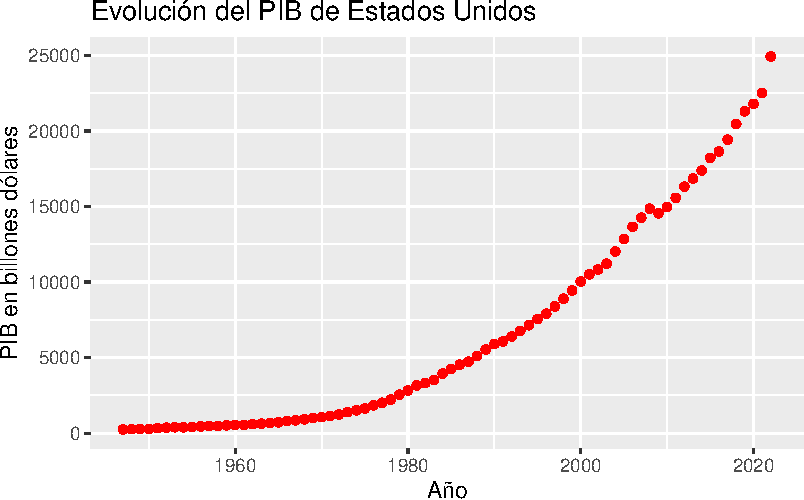
\includegraphics[keepaspectratio]{06-regresion_files/figure-pdf/unnamed-chunk-25-1.pdf}}

  A la vista de la forma de la nube de puntos parece que la evolución
  del PIB es exponencial.

  \end{tcolorbox}
\item
  Dibujar el diagrama de dispersión del logaritmo del PIB y los años.

  \begin{tcolorbox}[enhanced jigsaw, breakable, toptitle=1mm, colbacktitle=quarto-callout-tip-color!10!white, rightrule=.15mm, opacityback=0, opacitybacktitle=0.6, titlerule=0mm, coltitle=black, colframe=quarto-callout-tip-color-frame, colback=white, bottomtitle=1mm, leftrule=.75mm, toprule=.15mm, title=\textcolor{quarto-callout-tip-color}{\faLightbulb}\hspace{0.5em}{Solución}, arc=.35mm, bottomrule=.15mm, left=2mm]

\begin{Shaded}
\begin{Highlighting}[]
\FunctionTok{library}\NormalTok{(dplyr)}
\NormalTok{df }\OtherTok{\textless{}{-}} \FunctionTok{mutate}\NormalTok{(df, }\AttributeTok{logPIB =} \FunctionTok{log}\NormalTok{(PIB)) }
\FunctionTok{ggplot}\NormalTok{(df, }\FunctionTok{aes}\NormalTok{(}\AttributeTok{x =}\NormalTok{ Año, }\AttributeTok{y =}\NormalTok{ logPIB)) }\SpecialCharTok{+}
        \FunctionTok{geom\_point}\NormalTok{(}\AttributeTok{col =} \StringTok{"red"}\NormalTok{) }\SpecialCharTok{+}
        \FunctionTok{labs}\NormalTok{(}\AttributeTok{title =} \StringTok{"Evolución del PIB de Estados Unidos"}\NormalTok{, }\AttributeTok{x =} \StringTok{"Año"}\NormalTok{, }\AttributeTok{y =} \StringTok{"Logaritmo del PIB en billones dólares"}\NormalTok{)}
\end{Highlighting}
\end{Shaded}

  \pandocbounded{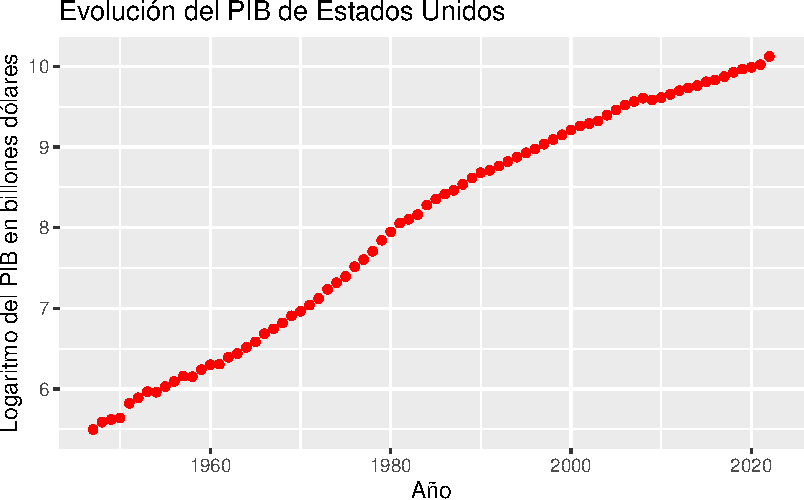
\includegraphics[keepaspectratio]{06-regresion_files/figure-pdf/unnamed-chunk-26-1.pdf}}

  La nube de puntos tienen una clara forma lineal, lo que confirma que
  la evolución del PIB es exponencial.

  \end{tcolorbox}
\item
  Calcular el modelo de regresión exponencial del PIB sobre los años.

  \begin{tcolorbox}[enhanced jigsaw, breakable, toptitle=1mm, colbacktitle=quarto-callout-tip-color!10!white, rightrule=.15mm, opacityback=0, opacitybacktitle=0.6, titlerule=0mm, coltitle=black, colframe=quarto-callout-tip-color-frame, colback=white, bottomtitle=1mm, leftrule=.75mm, toprule=.15mm, title=\textcolor{quarto-callout-tip-color}{\faLightbulb}\hspace{0.5em}{Solución}, arc=.35mm, bottomrule=.15mm, left=2mm]

\begin{Shaded}
\begin{Highlighting}[]
\NormalTok{recta\_logPIB\_años }\OtherTok{\textless{}{-}} \FunctionTok{lm}\NormalTok{(}\FunctionTok{log}\NormalTok{(PIB) }\SpecialCharTok{\textasciitilde{}}\NormalTok{ Año, df) }
\FunctionTok{summary}\NormalTok{(recta\_logPIB\_años)}
\end{Highlighting}
\end{Shaded}

\begin{verbatim}

Call:
lm(formula = log(PIB) ~ Año, data = df)

Residuals:
     Min       1Q   Median       3Q      Max 
-0.39115 -0.13495 -0.03532  0.17693  0.29436 

Coefficients:
              Estimate Std. Error t value Pr(>|t|)    
(Intercept) -1.215e+02  1.951e+00  -62.27   <2e-16 ***
Año          6.527e-02  9.832e-04   66.39   <2e-16 ***
---
Signif. codes:  0 '***' 0.001 '**' 0.01 '*' 0.05 '.' 0.1 ' ' 1

Residual standard error: 0.188 on 74 degrees of freedom
Multiple R-squared:  0.9835,    Adjusted R-squared:  0.9833 
F-statistic:  4407 on 1 and 74 DF,  p-value: < 2.2e-16
\end{verbatim}

  El modelo de regresión exponencial que mejor explica la evolución del
  PIB es \(\textsf{PIB}= e^{-121.4998223 + 0.065271 \textsf{Año}}\).

  \end{tcolorbox}
\item
  ¿Cuál es la tasa de crecimiento porcentual anual del PIB?

  \begin{tcolorbox}[enhanced jigsaw, breakable, toptitle=1mm, colbacktitle=quarto-callout-tip-color!10!white, rightrule=.15mm, opacityback=0, opacitybacktitle=0.6, titlerule=0mm, coltitle=black, colframe=quarto-callout-tip-color-frame, colback=white, bottomtitle=1mm, leftrule=.75mm, toprule=.15mm, title=\textcolor{quarto-callout-tip-color}{\faLightbulb}\hspace{0.5em}{Solución}, arc=.35mm, bottomrule=.15mm, left=2mm]

\begin{Shaded}
\begin{Highlighting}[]
\FunctionTok{cat}\NormalTok{(}\FunctionTok{paste}\NormalTok{(}\StringTok{"Coeficiente de regresión del logaritmo del PIB sobre los años:"}\NormalTok{, recta\_logPIB\_años}\SpecialCharTok{$}\NormalTok{coefficients[[}\StringTok{"Año"}\NormalTok{]]))}
\end{Highlighting}
\end{Shaded}

\begin{verbatim}
Coeficiente de regresión del logaritmo del PIB sobre los años: 0.0652710244896025
\end{verbatim}

  El coeficiente de regresión de los suspensos sobre las horas de
  estudio vale 0.065271, lo que indica que la tasa de crecimiento anual
  del PIB es 6.5271024\%.

  \end{tcolorbox}
\item
  Dibujar el modelo de regresión exponencial sobre el diagrama de
  dispersión.

  \begin{tcolorbox}[enhanced jigsaw, breakable, toptitle=1mm, colbacktitle=quarto-callout-tip-color!10!white, rightrule=.15mm, opacityback=0, opacitybacktitle=0.6, titlerule=0mm, coltitle=black, colframe=quarto-callout-tip-color-frame, colback=white, bottomtitle=1mm, leftrule=.75mm, toprule=.15mm, title=\textcolor{quarto-callout-tip-color}{\faLightbulb}\hspace{0.5em}{Solución}, arc=.35mm, bottomrule=.15mm, left=2mm]

\begin{Shaded}
\begin{Highlighting}[]
\FunctionTok{library}\NormalTok{(ggplot2)}
\FunctionTok{ggplot}\NormalTok{(df, }\FunctionTok{aes}\NormalTok{(}\AttributeTok{x =}\NormalTok{ Año, }\AttributeTok{y =}\NormalTok{ PIB)) }\SpecialCharTok{+}
        \FunctionTok{geom\_point}\NormalTok{(}\AttributeTok{col =} \StringTok{"red"}\NormalTok{) }\SpecialCharTok{+}
        \FunctionTok{geom\_smooth}\NormalTok{(}\AttributeTok{method =} \StringTok{"glm"}\NormalTok{, }\AttributeTok{method.args =} \FunctionTok{list}\NormalTok{(}\AttributeTok{family=}\FunctionTok{gaussian}\NormalTok{(}\AttributeTok{link=}\StringTok{"log"}\NormalTok{)))}
\end{Highlighting}
\end{Shaded}

  \pandocbounded{\includegraphics[keepaspectratio]{06-regresion_files/figure-pdf/unnamed-chunk-29-1.pdf}}

\begin{Shaded}
\begin{Highlighting}[]
        \FunctionTok{labs}\NormalTok{(}\AttributeTok{title =} \StringTok{"Evolución del PIB de Estados Unidos"}\NormalTok{, }\AttributeTok{x =} \StringTok{"Año"}\NormalTok{, }\AttributeTok{y =} \StringTok{"Logaritmo del PIB en billones dólares"}\NormalTok{)}
\end{Highlighting}
\end{Shaded}

\begin{verbatim}
$x
[1] "Año"

$y
[1] "Logaritmo del PIB en billones dólares"

$title
[1] "Evolución del PIB de Estados Unidos"

attr(,"class")
[1] "labels"
\end{verbatim}

  En este caso el ajuste no es perfecto, ya que es imposible que la
  recta pase por todos los puntos como ocurría en el ejercicio anterior.
  Por tanto, el ajuste es peor.

  \end{tcolorbox}
\item
  ¿Es el modelo de regresión exponencial un buen modelo para explicar la
  evolución del PIB?

  \begin{tcolorbox}[enhanced jigsaw, breakable, toptitle=1mm, colbacktitle=quarto-callout-tip-color!10!white, rightrule=.15mm, opacityback=0, opacitybacktitle=0.6, titlerule=0mm, coltitle=black, colframe=quarto-callout-tip-color-frame, colback=white, bottomtitle=1mm, leftrule=.75mm, toprule=.15mm, title=\textcolor{quarto-callout-tip-color}{\faLightbulb}\hspace{0.5em}{Solución}, arc=.35mm, bottomrule=.15mm, left=2mm]

\begin{Shaded}
\begin{Highlighting}[]
\FunctionTok{cat}\NormalTok{(}\FunctionTok{paste}\NormalTok{(}\StringTok{"Coeficiente de determinación exponencial R²:"}\NormalTok{, }\FunctionTok{summary}\NormalTok{(recta\_logPIB\_años)}\SpecialCharTok{$}\NormalTok{r.squared))}
\end{Highlighting}
\end{Shaded}

\begin{verbatim}
Coeficiente de determinación exponencial R²: 0.983487569858149
\end{verbatim}

  Como el coeficiente de determinación lineal vale 0.9834876 que está
  bastante próximo a 1, el ajuste es bueno, y el modelo exponencial
  explica muy bien la evolución del PIB.

  \end{tcolorbox}
\item
  Utilizar el modelo de regresión exponencial para predecir el PIB del
  año 2024. ¿Es fiable esta predicción?

  \begin{tcolorbox}[enhanced jigsaw, breakable, toptitle=1mm, colbacktitle=quarto-callout-tip-color!10!white, rightrule=.15mm, opacityback=0, opacitybacktitle=0.6, titlerule=0mm, coltitle=black, colframe=quarto-callout-tip-color-frame, colback=white, bottomtitle=1mm, leftrule=.75mm, toprule=.15mm, title=\textcolor{quarto-callout-tip-color}{\faLightbulb}\hspace{0.5em}{Solución}, arc=.35mm, bottomrule=.15mm, left=2mm]

\begin{Shaded}
\begin{Highlighting}[]
\CommentTok{\# El modelo exponencial devuelve el logaritmo del PIB, por lo que hay que aplicar la función exponencial para obtener el PIB.}
\FunctionTok{exp}\NormalTok{(}\FunctionTok{predict.lm}\NormalTok{(recta\_logPIB\_años, }\AttributeTok{newdata =} \FunctionTok{list}\NormalTok{(Año }\OtherTok{=} \DecValTok{2024}\NormalTok{)))}
\end{Highlighting}
\end{Shaded}

\begin{verbatim}
      1 
40486.8 
\end{verbatim}

  La predicción será fiable ya que el coeficiente de determinación está
  próximo a 1, el tamaño de la muestra no es muy pequeño y el año para
  el que se realiza la predicción no está lejos del rango de años de la
  muestra.

  \end{tcolorbox}
\item
  ¿Cuándo se alcanzará un PIB de 50000 billones de dólares?

  \begin{tcolorbox}[enhanced jigsaw, breakable, toptitle=1mm, colbacktitle=quarto-callout-tip-color!10!white, rightrule=.15mm, opacityback=0, opacitybacktitle=0.6, titlerule=0mm, coltitle=black, colframe=quarto-callout-tip-color-frame, colback=white, bottomtitle=1mm, leftrule=.75mm, toprule=.15mm, title=\textcolor{quarto-callout-tip-color}{\faLightbulb}\hspace{0.5em}{Solución}, arc=.35mm, bottomrule=.15mm, left=2mm]

  Como ahora queremos predecir el año en el que se alcanzará el PIB
  dado, necesitamos construir el modelo de regresión de los años sobre
  el PIB. Como la relación entre el PIB y los años es exponencial, la
  relación entre los años y el PIB será la inversa, es decir, el modelo
  logarítmico.

\begin{Shaded}
\begin{Highlighting}[]
\NormalTok{log\_años\_PIB }\OtherTok{\textless{}{-}} \FunctionTok{lm}\NormalTok{(Año }\SpecialCharTok{\textasciitilde{}} \FunctionTok{log}\NormalTok{(PIB), df) }
\FunctionTok{summary}\NormalTok{(log\_años\_PIB)}
\end{Highlighting}
\end{Shaded}

\begin{verbatim}

Call:
lm(formula = Año ~ log(PIB), data = df)

Residuals:
    Min      1Q  Median      3Q     Max 
-4.4049 -2.5367  0.2662  1.7718  6.4965 

Coefficients:
            Estimate Std. Error t value Pr(>|t|)    
(Intercept) 1863.498      1.852 1006.29   <2e-16 ***
log(PIB)      15.068      0.227   66.39   <2e-16 ***
---
Signif. codes:  0 '***' 0.001 '**' 0.01 '*' 0.05 '.' 0.1 ' ' 1

Residual standard error: 2.857 on 74 degrees of freedom
Multiple R-squared:  0.9835,    Adjusted R-squared:  0.9833 
F-statistic:  4407 on 1 and 74 DF,  p-value: < 2.2e-16
\end{verbatim}

  El modelo de regresión logarítmico de los años sobre el PIB es
  \(\textsf{Año}= 1863.4980331 + 15.0677514 \log(\textsf{PIB})\).

\begin{Shaded}
\begin{Highlighting}[]
\FunctionTok{predict.lm}\NormalTok{(log\_años\_PIB, }\AttributeTok{newdata =} \FunctionTok{list}\NormalTok{(}\AttributeTok{PIB =} \DecValTok{50000}\NormalTok{))}
\end{Highlighting}
\end{Shaded}

\begin{verbatim}
       1 
2026.528 
\end{verbatim}

  \end{tcolorbox}
\end{enumerate}

\end{exercise}

\begin{exercise}[]\protect\hypertarget{exr-regresion-5}{}\label{exr-regresion-5}

El fichero \href{datos/dieta.csv}{\texttt{dieta.csv}} contiene
información sobre el los kilos perdidos con una dieta de adelgazamiento.

\begin{enumerate}
\def\labelenumi{\alph{enumi}.}
\item
  Crear un data frame con los datos de la dieta a partir del fichero
  \href{https://aprendeconalf.es/estadistica-practicas-r/datos/dieta.csv}{\texttt{dieta.csv}}.

  \begin{tcolorbox}[enhanced jigsaw, breakable, toptitle=1mm, colbacktitle=quarto-callout-tip-color!10!white, rightrule=.15mm, opacityback=0, opacitybacktitle=0.6, titlerule=0mm, coltitle=black, colframe=quarto-callout-tip-color-frame, colback=white, bottomtitle=1mm, leftrule=.75mm, toprule=.15mm, title=\textcolor{quarto-callout-tip-color}{\faLightbulb}\hspace{0.5em}{Solución}, arc=.35mm, bottomrule=.15mm, left=2mm]

\begin{Shaded}
\begin{Highlighting}[]
\FunctionTok{library}\NormalTok{(readr)}
\NormalTok{df }\OtherTok{\textless{}{-}} \FunctionTok{read\_csv}\NormalTok{(}\StringTok{"https://aprendeconalf.es/estadistica{-}practicas{-}r/datos/dieta.csv"}\NormalTok{)}
\NormalTok{df}
\end{Highlighting}
\end{Shaded}

\begin{verbatim}
# A tibble: 40 x 3
    dias peso.perdido ejercicio
   <dbl>        <dbl> <chr>    
 1    14         2.95 no       
 2    18         5.65 no       
 3    22         6.56 no       
 4    26         3.56 no       
 5    30         6.17 no       
 6    34         9.4  no       
 7    38        12.4  no       
 8    42        12.9  no       
 9    46        13.9  no       
10    50        10.8  no       
# i 30 more rows
\end{verbatim}

  \end{tcolorbox}
\item
  Dibujar el diagrama de dispersión de los kilos perdidos en función del
  número de días con la dieta. ¿Qué tipo de modelo de regresión se
  ajusta mejor a la nube de puntos?

  \begin{tcolorbox}[enhanced jigsaw, breakable, toptitle=1mm, colbacktitle=quarto-callout-tip-color!10!white, rightrule=.15mm, opacityback=0, opacitybacktitle=0.6, titlerule=0mm, coltitle=black, colframe=quarto-callout-tip-color-frame, colback=white, bottomtitle=1mm, leftrule=.75mm, toprule=.15mm, title=\textcolor{quarto-callout-tip-color}{\faLightbulb}\hspace{0.5em}{Solución}, arc=.35mm, bottomrule=.15mm, left=2mm]

\begin{Shaded}
\begin{Highlighting}[]
\FunctionTok{library}\NormalTok{(ggplot2)}
\FunctionTok{ggplot}\NormalTok{(df, }\FunctionTok{aes}\NormalTok{(}\AttributeTok{x =}\NormalTok{ dias, }\AttributeTok{y =}\NormalTok{ peso.perdido)) }\SpecialCharTok{+}
    \FunctionTok{geom\_point}\NormalTok{(}\AttributeTok{col =} \StringTok{"red"}\NormalTok{) }\SpecialCharTok{+}
    \FunctionTok{labs}\NormalTok{(}\AttributeTok{title =} \StringTok{"Diagrama de dispersión del peso perdido y los días de dieta"}\NormalTok{, }\AttributeTok{x =} \StringTok{"Días de dieta"}\NormalTok{, }\AttributeTok{y =} \StringTok{"Peso perdido en Kg"}\NormalTok{)}
\end{Highlighting}
\end{Shaded}

  \pandocbounded{\includegraphics[keepaspectratio]{06-regresion_files/figure-pdf/unnamed-chunk-35-1.pdf}}

  La nube de puntos es bastante difusa aunque parece apreciarse una
  tendencia logarítmica o sigmoidal.

  \end{tcolorbox}
\item
  Calcular los coeficientes de determinación lineal, cuadrático,
  exponencial, logarítmico, potencial, inverso y sigmoidal. ¿Qué tipo de
  modelo explica mejor la relación entre los kilos perdidos y el número
  de días de dieta? ¿Qué porcentaje de la variabilidad de peso perdido
  explica el mejor modelo de regresión?

  \begin{tcolorbox}[enhanced jigsaw, breakable, toptitle=1mm, colbacktitle=quarto-callout-tip-color!10!white, rightrule=.15mm, opacityback=0, opacitybacktitle=0.6, titlerule=0mm, coltitle=black, colframe=quarto-callout-tip-color-frame, colback=white, bottomtitle=1mm, leftrule=.75mm, toprule=.15mm, title=\textcolor{quarto-callout-tip-color}{\faLightbulb}\hspace{0.5em}{Solución}, arc=.35mm, bottomrule=.15mm, left=2mm]

\begin{Shaded}
\begin{Highlighting}[]
\FunctionTok{library}\NormalTok{(dplyr)}
\FunctionTok{library}\NormalTok{(tidyr)}
\FunctionTok{library}\NormalTok{(purrr)}
\FunctionTok{library}\NormalTok{(broom)}
\FunctionTok{library}\NormalTok{(kableExtra)}
\CommentTok{\# Construimos un data frame con el ajuste de los modelos.}
\NormalTok{modelos }\OtherTok{\textless{}{-}} \FunctionTok{tibble}\NormalTok{(}
        \AttributeTok{Lineal =} \FunctionTok{list}\NormalTok{(}\FunctionTok{lm}\NormalTok{(peso.perdido }\SpecialCharTok{\textasciitilde{}}\NormalTok{ dias, df)),}
        \AttributeTok{Cuadratico =} \FunctionTok{list}\NormalTok{(}\FunctionTok{lm}\NormalTok{(peso.perdido }\SpecialCharTok{\textasciitilde{}}\NormalTok{ dias }\SpecialCharTok{+} \FunctionTok{I}\NormalTok{(dias}\SpecialCharTok{\^{}}\DecValTok{2}\NormalTok{), df)),}
        \AttributeTok{Exponencial =} \FunctionTok{list}\NormalTok{(}\FunctionTok{lm}\NormalTok{(}\FunctionTok{log}\NormalTok{(peso.perdido) }\SpecialCharTok{\textasciitilde{}}\NormalTok{ dias, df)),}
        \AttributeTok{Logaritmico =} \FunctionTok{list}\NormalTok{(}\FunctionTok{lm}\NormalTok{(peso.perdido }\SpecialCharTok{\textasciitilde{}} \FunctionTok{log}\NormalTok{(dias), df)),}
        \AttributeTok{Potencial =} \FunctionTok{list}\NormalTok{(}\FunctionTok{lm}\NormalTok{(}\FunctionTok{log}\NormalTok{(peso.perdido) }\SpecialCharTok{\textasciitilde{}} \FunctionTok{log}\NormalTok{(dias), df)),}
        \AttributeTok{Inverso =} \FunctionTok{list}\NormalTok{(}\FunctionTok{lm}\NormalTok{(peso.perdido }\SpecialCharTok{\textasciitilde{}} \FunctionTok{I}\NormalTok{(}\DecValTok{1}\SpecialCharTok{/}\NormalTok{dias), df)),}
        \AttributeTok{Sigmoidal =} \FunctionTok{list}\NormalTok{(}\FunctionTok{lm}\NormalTok{(}\FunctionTok{log}\NormalTok{(peso.perdido) }\SpecialCharTok{\textasciitilde{}} \FunctionTok{I}\NormalTok{(}\DecValTok{1}\SpecialCharTok{/}\NormalTok{dias), df)),}
\NormalTok{    )  }\SpecialCharTok{|\textgreater{}} 
    \CommentTok{\# }
    \CommentTok{\# Reestructuramos el data frame para tener todos los modelos en la misma columna.}
    \FunctionTok{pivot\_longer}\NormalTok{(}\FunctionTok{everything}\NormalTok{(), }\AttributeTok{names\_to =} \StringTok{"Tipo\_Modelo"}\NormalTok{, }\AttributeTok{values\_to =} \StringTok{"Modelo"}\NormalTok{)  }\SpecialCharTok{|\textgreater{}} 
    \CommentTok{\# Obtenemos un resumen del ajuste de cada modelo en formato organizado (se obtiene una lista con los parámetros que describen el ajuste de cada modelo).}
    \FunctionTok{mutate}\NormalTok{(}\AttributeTok{Resumen =} \FunctionTok{map}\NormalTok{(Modelo, glance)) }\SpecialCharTok{|\textgreater{}} 
    \CommentTok{\# Desanidamos el resumen (se obtiene una columna para cada parámetro del resumen del ajuste de los modelos).}
    \FunctionTok{unnest}\NormalTok{(Resumen)  }\SpecialCharTok{|\textgreater{}} 
    \CommentTok{\# Ordenamos el data frame por el coeficiente de determinación.}
    \FunctionTok{arrange}\NormalTok{(}\SpecialCharTok{{-}}\NormalTok{r.squared)}

\NormalTok{modelos  }\SpecialCharTok{|\textgreater{}}
    \FunctionTok{select}\NormalTok{(Tipo\_Modelo, r.squared)  }\SpecialCharTok{|\textgreater{}} 
    \FunctionTok{kable}\NormalTok{(}\AttributeTok{col.names =} \FunctionTok{c}\NormalTok{(}\StringTok{"Tipo de Modelo"}\NormalTok{, }\StringTok{"R²"}\NormalTok{)) }\SpecialCharTok{|\textgreater{}}
    \FunctionTok{kable\_styling}\NormalTok{(}\AttributeTok{full\_width =}\NormalTok{ F)}
\end{Highlighting}
\end{Shaded}

  \begin{longtable*}[t]{lr}
  \toprule
  Tipo de Modelo & R²\\
  \midrule
  Sigmoidal & 0.6662170\\
  Potencial & 0.5684490\\
  Inverso & 0.5583853\\
  Cuadratico & 0.5397848\\
  Logaritmico & 0.5254856\\
  \addlinespace
  Lineal & 0.4356390\\
  Exponencial & 0.4308936\\
  \bottomrule
  \end{longtable*}

  El mejor modelo es el Sigmoidal que explica el 66.6216965388749\% de
  la variabilidad del peso perdido.

  \end{tcolorbox}
\item
  Dibujar el diagrama de dispersión de los kilos perdidos en función del
  número de días con la dieta según si la persona hace ejercicio o no.
  ¿Qué conclusiones se pueden sacar?

  \begin{tcolorbox}[enhanced jigsaw, breakable, toptitle=1mm, colbacktitle=quarto-callout-tip-color!10!white, rightrule=.15mm, opacityback=0, opacitybacktitle=0.6, titlerule=0mm, coltitle=black, colframe=quarto-callout-tip-color-frame, colback=white, bottomtitle=1mm, leftrule=.75mm, toprule=.15mm, title=\textcolor{quarto-callout-tip-color}{\faLightbulb}\hspace{0.5em}{Solución}, arc=.35mm, bottomrule=.15mm, left=2mm]

\begin{Shaded}
\begin{Highlighting}[]
\FunctionTok{library}\NormalTok{(ggplot2)}
\FunctionTok{ggplot}\NormalTok{(df, }\FunctionTok{aes}\NormalTok{(}\AttributeTok{x =}\NormalTok{ dias, }\AttributeTok{y =}\NormalTok{ peso.perdido, }\AttributeTok{color =}\NormalTok{ ejercicio)) }\SpecialCharTok{+}
    \FunctionTok{geom\_point}\NormalTok{() }\SpecialCharTok{+}
    \FunctionTok{labs}\NormalTok{(}\AttributeTok{title =} \StringTok{"Diagrama de dispersión del peso perdido y los días de dieta"}\NormalTok{, }\AttributeTok{x =} \StringTok{"Días de dieta"}\NormalTok{, }\AttributeTok{y =} \StringTok{"Peso perdido en Kg"}\NormalTok{)}
\end{Highlighting}
\end{Shaded}

  \pandocbounded{\includegraphics[keepaspectratio]{06-regresion_files/figure-pdf/unnamed-chunk-37-1.pdf}}

  Claramente la nube de puntos de las personas que hacen ejercicio está
  por encima de la de los que no hacen ejercicio, lo que indica que
  hacer ejercicio favorece la pérdida de peso. Los más razonable es
  construir modelos de regresión para cada grupo.

  \end{tcolorbox}
\item
  ¿Qué tipo de modelo explica mejor la relación entre el peso perdido y
  los días de dieta en el grupo de las personas que hacen ejercicio? ¿Y
  en el grupo de las que no hacen ejercicio? ¿Han mejorado los modelos
  con respecto al modelo anterior?

  \begin{tcolorbox}[enhanced jigsaw, breakable, toptitle=1mm, colbacktitle=quarto-callout-tip-color!10!white, rightrule=.15mm, opacityback=0, opacitybacktitle=0.6, titlerule=0mm, coltitle=black, colframe=quarto-callout-tip-color-frame, colback=white, bottomtitle=1mm, leftrule=.75mm, toprule=.15mm, title=\textcolor{quarto-callout-tip-color}{\faLightbulb}\hspace{0.5em}{Solución}, arc=.35mm, bottomrule=.15mm, left=2mm]

\begin{Shaded}
\begin{Highlighting}[]
\NormalTok{modelos }\OtherTok{\textless{}{-}}\NormalTok{ df  }\SpecialCharTok{|\textgreater{}} 
    \CommentTok{\# Anidamos por la columna ejercicio.}
    \FunctionTok{nest\_by}\NormalTok{(ejercicio)  }\SpecialCharTok{|\textgreater{}} 
    \CommentTok{\# Ajustamos los modelos de regresión.}
    \FunctionTok{mutate}\NormalTok{(}
        \AttributeTok{Lineal =} \FunctionTok{list}\NormalTok{(}\FunctionTok{lm}\NormalTok{(peso.perdido }\SpecialCharTok{\textasciitilde{}}\NormalTok{ dias, data)),}
        \AttributeTok{Cuadratico =} \FunctionTok{list}\NormalTok{(}\FunctionTok{lm}\NormalTok{(peso.perdido }\SpecialCharTok{\textasciitilde{}}\NormalTok{ dias }\SpecialCharTok{+} \FunctionTok{I}\NormalTok{(dias}\SpecialCharTok{\^{}}\DecValTok{2}\NormalTok{), data)),}
        \AttributeTok{Exponencial =} \FunctionTok{list}\NormalTok{(}\FunctionTok{lm}\NormalTok{(}\FunctionTok{log}\NormalTok{(peso.perdido) }\SpecialCharTok{\textasciitilde{}}\NormalTok{ dias, data)),}
        \AttributeTok{Logaritmico =} \FunctionTok{list}\NormalTok{(}\FunctionTok{lm}\NormalTok{(peso.perdido }\SpecialCharTok{\textasciitilde{}} \FunctionTok{log}\NormalTok{(dias), data)),}
        \AttributeTok{Potencial =} \FunctionTok{list}\NormalTok{(}\FunctionTok{lm}\NormalTok{(}\FunctionTok{log}\NormalTok{(peso.perdido) }\SpecialCharTok{\textasciitilde{}} \FunctionTok{log}\NormalTok{(dias), data)),}
        \AttributeTok{Inverso =} \FunctionTok{list}\NormalTok{(}\FunctionTok{lm}\NormalTok{(peso.perdido }\SpecialCharTok{\textasciitilde{}} \FunctionTok{I}\NormalTok{(}\DecValTok{1}\SpecialCharTok{/}\NormalTok{dias), data)),}
        \AttributeTok{Sigmoidal =} \FunctionTok{list}\NormalTok{(}\FunctionTok{lm}\NormalTok{(}\FunctionTok{log}\NormalTok{(peso.perdido) }\SpecialCharTok{\textasciitilde{}} \FunctionTok{I}\NormalTok{(}\DecValTok{1}\SpecialCharTok{/}\NormalTok{dias), data)),}
\NormalTok{    )  }\SpecialCharTok{|\textgreater{}} 
    \CommentTok{\# Reestructuramos el data frame para tener todos los modelos en la misma columna.}
    \FunctionTok{pivot\_longer}\NormalTok{(}\SpecialCharTok{{-}}\FunctionTok{c}\NormalTok{(ejercicio, data), }\AttributeTok{names\_to =} \StringTok{"Tipo\_Modelo"}\NormalTok{, }\AttributeTok{values\_to =} \StringTok{"Modelo"}\NormalTok{)  }\SpecialCharTok{|\textgreater{}} 
    \CommentTok{\# Obtenemos un resumen del ajuste de cada modelo en formato organizado (se obtiene una lista con los parámetros que describen el ajuste de cada modelo).}
    \FunctionTok{mutate}\NormalTok{(}\AttributeTok{Resumen =} \FunctionTok{map}\NormalTok{(Modelo, glance)) }\SpecialCharTok{|\textgreater{}} 
    \CommentTok{\# Desanidamos el resumen (se obtiene una columna para cada parámetro del resumen del ajuste de los modelos).}
    \FunctionTok{unnest}\NormalTok{(Resumen)  }\SpecialCharTok{|\textgreater{}} 
    \CommentTok{\# Ordenamos el data frame por la columna ejercicio y por el coeficiente de determinación.}
    \FunctionTok{arrange}\NormalTok{(ejercicio, }\SpecialCharTok{{-}}\NormalTok{r.squared)  }
\NormalTok{modelos }\SpecialCharTok{|\textgreater{}} 
    \FunctionTok{select}\NormalTok{(ejercicio, Tipo\_Modelo, r.squared)  }\SpecialCharTok{|\textgreater{}} 
    \FunctionTok{kable}\NormalTok{(}\AttributeTok{col.names =} \FunctionTok{c}\NormalTok{(}\StringTok{"Ejercicio"}\NormalTok{, }\StringTok{"Tipo de Modelo"}\NormalTok{, }\StringTok{"R²"}\NormalTok{)) }\SpecialCharTok{|\textgreater{}}
    \FunctionTok{pack\_rows}\NormalTok{(}\AttributeTok{index =} \FunctionTok{table}\NormalTok{(modelos}\SpecialCharTok{$}\NormalTok{ejercicio))  }\SpecialCharTok{|\textgreater{}} 
    \FunctionTok{kable\_styling}\NormalTok{(}\AttributeTok{full\_width =}\NormalTok{ F)}
\end{Highlighting}
\end{Shaded}

  \begin{longtable*}[t]{llr}
  \toprule
  Ejercicio & Tipo de Modelo & R²\\
  \midrule
  \addlinespace[0.3em]
  \multicolumn{3}{l}{\textbf{no}}\\
  \hspace{1em}no & Sigmoidal & 0.7401212\\
  \hspace{1em}no & Cuadratico & 0.7100610\\
  \hspace{1em}no & Inverso & 0.6796880\\
  \hspace{1em}no & Potencial & 0.6700051\\
  \hspace{1em}no & Logaritmico & 0.6494521\\
  \hspace{1em}no & Lineal & 0.5286338\\
  \hspace{1em}no & Exponencial & 0.5222832\\
  \addlinespace[0.3em]
  \multicolumn{3}{l}{\textbf{si}}\\
  \hspace{1em}si & Inverso & 0.8470993\\
  \hspace{1em}si & Sigmoidal & 0.8305013\\
  \hspace{1em}si & Logaritmico & 0.7885173\\
  \hspace{1em}si & Cuadratico & 0.7791671\\
  \hspace{1em}si & Potencial & 0.6704843\\
  \hspace{1em}si & Lineal & 0.6623502\\
  \hspace{1em}si & Exponencial & 0.4945564\\
  \bottomrule
  \end{longtable*}

  El mejor modelo en el grupo de los que hacen ejercicio es el inverso y
  en el grupo de los que no el sigmoidal. Los modelos han mejorado
  bastante con respecto al modelo anterior, sobre todo el del grupo de
  personas que hace ejercicio.

  \end{tcolorbox}
\item
  Construir el mejor modelo de regresión del peso perdido sobre los días
  de dieta para el grupo de las personas que hacen ejercicio y para el
  grupo de las que no.

  \begin{tcolorbox}[enhanced jigsaw, breakable, toptitle=1mm, colbacktitle=quarto-callout-tip-color!10!white, rightrule=.15mm, opacityback=0, opacitybacktitle=0.6, titlerule=0mm, coltitle=black, colframe=quarto-callout-tip-color-frame, colback=white, bottomtitle=1mm, leftrule=.75mm, toprule=.15mm, title=\textcolor{quarto-callout-tip-color}{\faLightbulb}\hspace{0.5em}{Solución}, arc=.35mm, bottomrule=.15mm, left=2mm]

  Construimos el modelo inverso para el grupo de las personas que hacen
  ejercicio.

\begin{Shaded}
\begin{Highlighting}[]
\NormalTok{inverso\_ejercicio }\OtherTok{\textless{}{-}} \FunctionTok{lm}\NormalTok{(peso.perdido }\SpecialCharTok{\textasciitilde{}} \FunctionTok{I}\NormalTok{(}\DecValTok{1}\SpecialCharTok{/}\NormalTok{dias), df[df}\SpecialCharTok{$}\NormalTok{ejercicio }\SpecialCharTok{==} \StringTok{"si"}\NormalTok{, ])}
\FunctionTok{summary}\NormalTok{(inverso\_ejercicio)}
\end{Highlighting}
\end{Shaded}

\begin{verbatim}

Call:
lm(formula = peso.perdido ~ I(1/dias), data = df[df$ejercicio == 
    "si", ])

Residuals:
    Min      1Q  Median      3Q     Max 
-3.1866 -1.3268  0.0011  0.9810  4.1456 

Coefficients:
             Estimate Std. Error t value Pr(>|t|)    
(Intercept)   21.5655     0.7653  28.181 2.42e-16 ***
I(1/dias)   -255.2249    25.5579  -9.986 9.12e-09 ***
---
Signif. codes:  0 '***' 0.001 '**' 0.01 '*' 0.05 '.' 0.1 ' ' 1

Residual standard error: 1.811 on 18 degrees of freedom
Multiple R-squared:  0.8471,    Adjusted R-squared:  0.8386 
F-statistic: 99.72 on 1 and 18 DF,  p-value: 9.123e-09
\end{verbatim}

  Y ahora el modelo sigmoidal para el grupo de las personas que no hacen
  ejercicio.

\begin{Shaded}
\begin{Highlighting}[]
\NormalTok{sigmoidal\_no\_ejercicio }\OtherTok{\textless{}{-}} \FunctionTok{lm}\NormalTok{(}\FunctionTok{log}\NormalTok{(peso.perdido) }\SpecialCharTok{\textasciitilde{}} \FunctionTok{I}\NormalTok{(}\DecValTok{1}\SpecialCharTok{/}\NormalTok{dias), df[df}\SpecialCharTok{$}\NormalTok{ejercicio }\SpecialCharTok{==} \StringTok{"no"}\NormalTok{, ])}
\FunctionTok{summary}\NormalTok{(sigmoidal\_no\_ejercicio)}
\end{Highlighting}
\end{Shaded}

\begin{verbatim}

Call:
lm(formula = log(peso.perdido) ~ I(1/dias), data = df[df$ejercicio == 
    "no", ])

Residuals:
     Min       1Q   Median       3Q      Max 
-0.66026 -0.07192  0.04678  0.13142  0.29633 

Coefficients:
            Estimate Std. Error t value Pr(>|t|)    
(Intercept)   2.8694     0.1021   28.09 2.55e-16 ***
I(1/dias)   -24.4226     3.4111   -7.16 1.15e-06 ***
---
Signif. codes:  0 '***' 0.001 '**' 0.01 '*' 0.05 '.' 0.1 ' ' 1

Residual standard error: 0.2417 on 18 degrees of freedom
Multiple R-squared:  0.7401,    Adjusted R-squared:  0.7257 
F-statistic: 51.26 on 1 and 18 DF,  p-value: 1.146e-06
\end{verbatim}

  \end{tcolorbox}
\item
  Según los mejores modelos de regresión en cada caso, ¿cuántos kilos
  perderá una persona que hace ejercicio tras 100 días de dieta? ¿Y una
  que no hace ejercicio?

  \begin{tcolorbox}[enhanced jigsaw, breakable, toptitle=1mm, colbacktitle=quarto-callout-tip-color!10!white, rightrule=.15mm, opacityback=0, opacitybacktitle=0.6, titlerule=0mm, coltitle=black, colframe=quarto-callout-tip-color-frame, colback=white, bottomtitle=1mm, leftrule=.75mm, toprule=.15mm, title=\textcolor{quarto-callout-tip-color}{\faLightbulb}\hspace{0.5em}{Solución}, arc=.35mm, bottomrule=.15mm, left=2mm]

  Hacemos primero la predicción del peso perdido para la persona que
  hace ejercicio usando el modelo inverso.

\begin{Shaded}
\begin{Highlighting}[]
\FunctionTok{predict.lm}\NormalTok{(inverso\_ejercicio, }\AttributeTok{newdata =} \FunctionTok{list}\NormalTok{(}\AttributeTok{dias =} \DecValTok{100}\NormalTok{))}
\end{Highlighting}
\end{Shaded}

\begin{verbatim}
       1 
19.01329 
\end{verbatim}

  Y ahora hacemos la predicción del peso perdido para la persona que no
  hace ejercicio usando el modelo sigmoidal.

\begin{Shaded}
\begin{Highlighting}[]
\CommentTok{\# El modelo sigmoidal devuelve el logaritmo del peso perdido por lo que hay que aplicar la función exponencial para obtener el peso perdido.}
\FunctionTok{exp}\NormalTok{(}\FunctionTok{predict.lm}\NormalTok{(sigmoidal\_no\_ejercicio, }\AttributeTok{newdata =} \FunctionTok{list}\NormalTok{(}\AttributeTok{dias =} \DecValTok{100}\NormalTok{)))}
\end{Highlighting}
\end{Shaded}

\begin{verbatim}
       1 
13.80634 
\end{verbatim}

  \end{tcolorbox}
\end{enumerate}

\end{exercise}

\section{Ejercicios propuestos}\label{ejercicios-propuestos-4}

\begin{exercise}[]\protect\hypertarget{exr-regresion-6}{}\label{exr-regresion-6}

El conjunto de datos
\href{https://aprendeconalf.es/estadistica-practicas-r/datos/neonatos.csv}{\texttt{neonatos}}
contiene información sobre una muestra de 320 recién nacidos en un
hospital durante un año que cumplieron el tiempo normal de gestación.

\begin{enumerate}
\def\labelenumi{\alph{enumi}.}
\item
  Crear un data frame a con los datos de los neonatos a partir del
  fichero anterior.
\item
  Construir la recta de regresión del peso de los recién nacidos sobre
  el número de cigarros fumados al día por las madres. ¿Existe una
  relación lineal fuerte entre el peso y el número de cigarros?
\item
  Dibujar la recta de regresión calculada en el apartado anterior. ¿Por
  qué la recta no se ajusta bien a la nube de puntos?
\item
  Calcular y dibujar la recta de regresión del peso de los recién
  nacidos sobre el número de cigarros fumados al día por las madres en
  el grupo de las madres que si fumaron durante el embarazo. ¿Es este
  modelo mejor o pero que la recta del apartado anterior?
\item
  Según este modelo, ¿cuánto disminuirá el peso del recién nacido por
  cada cigarro más diario que fume la madre?
\item
  Según el modelo anterior, ¿qué peso tendrá un recién nacido de una
  madre que ha fumado 5 cigarros diarios durante el embarazo? ¿Y si la
  madre ha fumado 30 cigarros diarios durante el embarazo? ¿Son fiables
  estas predicciones?
\item
  ¿Existe la misma relación lineal entre el peso de los recién nacidos y
  el número de cigarros fumados al día por las madres que fumaron
  durante el embarazo en el grupo de las madres menores de 20 y en el
  grupo de las madres mayores de 20? ¿Qué se puede concluir?
\end{enumerate}

\end{exercise}

\begin{exercise}[]\protect\hypertarget{exr-regresion-7}{}\label{exr-regresion-7}

El conjunto de datos
\href{https://aprendeconalf.es/estadistica-practicas-r/datos/edad-estatura.csv}{\texttt{edad.estatura}}
contiene la edad y la estatura de 30 personas.

\begin{enumerate}
\def\labelenumi{\alph{enumi}.}
\item
  Crear un data frame con los datos de las edades y las estaturas a
  partir del fichero anterior.
\item
  Calcular la recta de regresión de la estatura sobre la edad. ¿Es un
  buen modelo la recta de regresión?
\item
  Dibujar el diagrama de dispersión de la estatura sobre la edad.
  ¿Alrededor de qué edad se observa un cambio en la tendencia?
\item
  Recodificar la variable edad en dos grupos para mayores y menores de
  20 años.
\item
  Calcular la recta de regresión de la estatura sobre la edad para cada
  grupo de edad. ¿En qué grupo explica mejor la recta de regresión la
  relación entre la estatura y la edad?
\item
  Dibujar las rectas de regresión anteriores.
\item
  ¿Qué estatura se espera que tenga una persona de 14 años? ¿Y una de
  38?
\end{enumerate}

\end{exercise}

\begin{exercise}[]\protect\hypertarget{exr-regresion-8}{}\label{exr-regresion-8}

El conjunto de datos \texttt{gapminder} del paquete \texttt{gapminder}
contiene información sobre la esperanza de vida, la población, y el PIB
per cápita en dólares PPP de los principales países en un rango de años.

\begin{enumerate}
\def\labelenumi{\alph{enumi}.}
\item
  Instalar el paquete \texttt{gapminder} y cargarlo.
\item
  ¿Qué tipo de modelo explica mejor la evolución de la población con los
  años? Construir ese modelo.
\item
  ¿Qué tipo de modelo explica mejor la relación entre la esperanza de
  vida y el PIB per cápita?
\item
  ¿Qué tipo de modelo explica mejor la relación entre la esperanza de
  vida y el PIB r cápita para cada continente? Construir el mejor modelo
  en cada caso y utilizarlo para predecir la esperanza de vida de una
  persona de cada continente con un PIB per cápita de 1000 dólares PPP.
\end{enumerate}

\end{exercise}

\bookmarksetup{startatroot}

\chapter{Distribuciones de
probabilidad}\label{distribuciones-de-probabilidad}

\section{Ejercicios Resueltos}\label{ejercicios-resueltos-5}

Para la realización de esta práctica se requieren los siguientes
paquetes:

\begin{Shaded}
\begin{Highlighting}[]
\FunctionTok{library}\NormalTok{(tidyverse) }
\CommentTok{\# Incluye los siguientes paquetes:}
\CommentTok{\# {-} dplyr: para el preprocesamiento y manipulación de datos.}
\CommentTok{\# {-} ggplot2: para la representación gráfica.}
\CommentTok{\# {-} purrr: para aplicar funciones a vectores. }
\FunctionTok{library}\NormalTok{(extraDistr) }\CommentTok{\# para distribuciones de probabilidad adicionales.}
\FunctionTok{library}\NormalTok{(knitr) }\CommentTok{\# para el formateo de tablas.}
\FunctionTok{library}\NormalTok{(kableExtra) }\CommentTok{\# para personalizar el formato de las tablas.}
\end{Highlighting}
\end{Shaded}

\begin{exercise}[]\protect\hypertarget{exr-distribuciones-probabilidad-1}{}\label{exr-distribuciones-probabilidad-1}

Sea \(X\) la variable que mide el resultado obtenido al lanzar un dado.

\begin{enumerate}
\def\labelenumi{\alph{enumi}.}
\item
  ¿Qué tipo de modelo de distribución de probabilidad sigue \(X\)?
  Construir su función de probabilidad.

  \begin{tcolorbox}[enhanced jigsaw, breakable, toptitle=1mm, colbacktitle=quarto-callout-tip-color!10!white, rightrule=.15mm, opacityback=0, opacitybacktitle=0.6, titlerule=0mm, coltitle=black, colframe=quarto-callout-tip-color-frame, colback=white, bottomtitle=1mm, leftrule=.75mm, toprule=.15mm, title=\textcolor{quarto-callout-tip-color}{\faLightbulb}\hspace{0.5em}{Solución}, arc=.35mm, bottomrule=.15mm, left=2mm]

  Se trata de una
  \href{https://es.wikipedia.org/wiki/Distribuci\%C3\%B3n_uniforme_discreta}{distribución
  uniforme discreta} \(U(1, 6)\). Para calcular probabilidades con el
  modelo uniforme discreto se utiliza la función
  \href{https://www.rdocumentation.org/packages/extraDistr/versions/1.9.1/topics/DiscreteUniform}{\texttt{ddunif(x,\ min,\ max)}}
  del paquete \texttt{extraDistr}, donde \texttt{min} es el mínimo valor
  que puede tomar la variable, \texttt{max} es el máximo valor que puede
  tomar la variable y \texttt{x} es el valor de la variable.

\begin{Shaded}
\begin{Highlighting}[]
\FunctionTok{library}\NormalTok{(extraDistr)}
\FunctionTok{library}\NormalTok{(kableExtra)}
\NormalTok{x }\OtherTok{\textless{}{-}} \DecValTok{1}\SpecialCharTok{:}\DecValTok{6}
\NormalTok{f }\OtherTok{\textless{}{-}} \FunctionTok{ddunif}\NormalTok{(x, }\DecValTok{1}\NormalTok{, }\DecValTok{6}\NormalTok{)}
\NormalTok{df }\OtherTok{\textless{}{-}} \FunctionTok{data.frame}\NormalTok{(x, f)}
\NormalTok{df }\SpecialCharTok{|\textgreater{}} 
    \FunctionTok{kable}\NormalTok{() }\SpecialCharTok{|\textgreater{}} 
    \FunctionTok{kable\_styling}\NormalTok{(}\AttributeTok{full\_width =}\NormalTok{ F)}
\end{Highlighting}
\end{Shaded}

  \begin{longtable*}[t]{rr}
  \toprule
  x & f\\
  \midrule
  1 & 0.1666667\\
  2 & 0.1666667\\
  3 & 0.1666667\\
  4 & 0.1666667\\
  5 & 0.1666667\\
  \addlinespace
  6 & 0.1666667\\
  \bottomrule
  \end{longtable*}

  \end{tcolorbox}
\item
  Dibujar la gráfica de la función de probabilidad del modelo de
  probabilidad anterior.

  \begin{tcolorbox}[enhanced jigsaw, breakable, toptitle=1mm, colbacktitle=quarto-callout-tip-color!10!white, rightrule=.15mm, opacityback=0, opacitybacktitle=0.6, titlerule=0mm, coltitle=black, colframe=quarto-callout-tip-color-frame, colback=white, bottomtitle=1mm, leftrule=.75mm, toprule=.15mm, title=\textcolor{quarto-callout-tip-color}{\faLightbulb}\hspace{0.5em}{Solución}, arc=.35mm, bottomrule=.15mm, left=2mm]

\begin{Shaded}
\begin{Highlighting}[]
\FunctionTok{library}\NormalTok{(ggplot2)}
\FunctionTok{ggplot}\NormalTok{(df, }\FunctionTok{aes}\NormalTok{(}\AttributeTok{x =}\NormalTok{ x, }\AttributeTok{y =}\NormalTok{ f)) }\SpecialCharTok{+}
    \FunctionTok{geom\_point}\NormalTok{(}\AttributeTok{color =} \StringTok{"steelblue"}\NormalTok{) }\SpecialCharTok{+}
    \FunctionTok{labs}\NormalTok{(}\AttributeTok{title =} \StringTok{"Función de probabilidad uniforme U(1,6)"}\NormalTok{, }\AttributeTok{x =} \StringTok{"Número obtenido"}\NormalTok{, }\AttributeTok{y =} \StringTok{"Probabilidad"}\NormalTok{)}
\end{Highlighting}
\end{Shaded}

  \pandocbounded{\includegraphics[keepaspectratio]{07-distribuciones-probabilidad_files/figure-pdf/unnamed-chunk-2-1.pdf}}

  \end{tcolorbox}
\item
  Simular el experimento aleatorio del lanzamiento de un dado. Repetir
  el lanzamiento un millón de veces y dibujar el diagrama de barras de
  la distribución de frecuencias resultante. ¿Se parece a la
  distribución de probabilidad anterior?

  \begin{tcolorbox}[enhanced jigsaw, breakable, toptitle=1mm, colbacktitle=quarto-callout-tip-color!10!white, rightrule=.15mm, opacityback=0, opacitybacktitle=0.6, titlerule=0mm, coltitle=black, colframe=quarto-callout-tip-color-frame, colback=white, bottomtitle=1mm, leftrule=.75mm, toprule=.15mm, title=\textcolor{quarto-callout-tip-color}{\faLightbulb}\hspace{0.5em}{Solución}, arc=.35mm, bottomrule=.15mm, left=2mm]

\begin{Shaded}
\begin{Highlighting}[]
\CommentTok{\# Fijamos una semilla de aleatorización para obtener resultados reproducibles.}
\FunctionTok{set.seed}\NormalTok{(}\DecValTok{123}\NormalTok{)}
\FunctionTok{data.frame}\NormalTok{(}\AttributeTok{x =} \FunctionTok{rdunif}\NormalTok{(}\DecValTok{10}\SpecialCharTok{\^{}}\DecValTok{6}\NormalTok{, }\DecValTok{1}\NormalTok{, }\DecValTok{6}\NormalTok{))  }\SpecialCharTok{|\textgreater{}} 
    \FunctionTok{ggplot}\NormalTok{(}\FunctionTok{aes}\NormalTok{(}\AttributeTok{x =}\NormalTok{ x)) }\SpecialCharTok{+}
    \FunctionTok{geom\_bar}\NormalTok{(}\FunctionTok{aes}\NormalTok{(}\AttributeTok{y =} \FunctionTok{after\_stat}\NormalTok{(count}\SpecialCharTok{/}\FunctionTok{sum}\NormalTok{(count))), }\AttributeTok{fill =} \StringTok{"steelblue"}\NormalTok{) }\SpecialCharTok{+}
    \FunctionTok{labs}\NormalTok{(}\AttributeTok{title =} \StringTok{"Distribución de frecuencias del lanzamiento de un dado"}\NormalTok{, }\AttributeTok{x =} \StringTok{"Número obtenido"}\NormalTok{, }\AttributeTok{y =} \StringTok{"Frecuencia relativa"}\NormalTok{)}
\end{Highlighting}
\end{Shaded}

  \pandocbounded{\includegraphics[keepaspectratio]{07-distribuciones-probabilidad_files/figure-pdf/unnamed-chunk-3-1.pdf}}

  La distribución experimental obtenida es casi idéntica a la
  distribución teórica del modelo uniforme \(U(1,6)\).

  \end{tcolorbox}
\end{enumerate}

\end{exercise}

\begin{exercise}[]\protect\hypertarget{exr-distribuciones-probabilidad-2}{}\label{exr-distribuciones-probabilidad-2}

Un test consta de 10 preguntas de opción múltiple con cuatro posibles
respuestas para cada pregunta.

\begin{enumerate}
\def\labelenumi{\alph{enumi}.}
\item
  ¿Qué tipo de modelo de distribución de probabilidad sigue la variable
  que mide el número de aciertos al responder todas las preguntas
  aleatoriamente? Construir su función de probabilidad.

  \begin{tcolorbox}[enhanced jigsaw, breakable, toptitle=1mm, colbacktitle=quarto-callout-tip-color!10!white, rightrule=.15mm, opacityback=0, opacitybacktitle=0.6, titlerule=0mm, coltitle=black, colframe=quarto-callout-tip-color-frame, colback=white, bottomtitle=1mm, leftrule=.75mm, toprule=.15mm, title=\textcolor{quarto-callout-tip-color}{\faLightbulb}\hspace{0.5em}{Solución}, arc=.35mm, bottomrule=.15mm, left=2mm]

  Se trata de una
  \href{https://es.wikipedia.org/wiki/Distribuci\%C3\%B3n_binomial}{distribución
  binomial} \(B(10, 0.25)\). Para calcular probabilidades con el modelo
  binomial se utiliza la función
  \href{https://www.rdocumentation.org/packages/stats/versions/3.3/topics/Binomial}{\texttt{dbinom(x,\ n,\ p)}}
  del paquete \texttt{stats}, donde \texttt{n} es el número de
  repeticiones, \texttt{p} es la probabilidad de éxito, y \texttt{x} es
  el valor de la variable.

\begin{Shaded}
\begin{Highlighting}[]
\FunctionTok{library}\NormalTok{(kableExtra)}
\NormalTok{x }\OtherTok{\textless{}{-}} \DecValTok{0}\SpecialCharTok{:}\DecValTok{10}
\NormalTok{f }\OtherTok{\textless{}{-}} \FunctionTok{dbinom}\NormalTok{(x, }\DecValTok{10}\NormalTok{, }\FloatTok{0.25}\NormalTok{)}
\NormalTok{df }\OtherTok{\textless{}{-}} \FunctionTok{data.frame}\NormalTok{(x, f)}
\NormalTok{df }\SpecialCharTok{|\textgreater{}} 
    \FunctionTok{kable}\NormalTok{() }\SpecialCharTok{|\textgreater{}} 
    \FunctionTok{kable\_styling}\NormalTok{(}\AttributeTok{full\_width =}\NormalTok{ F)}
\end{Highlighting}
\end{Shaded}

  \begin{longtable*}[t]{rr}
  \toprule
  x & f\\
  \midrule
  0 & 0.0563135\\
  1 & 0.1877117\\
  2 & 0.2815676\\
  3 & 0.2502823\\
  4 & 0.1459980\\
  \addlinespace
  5 & 0.0583992\\
  6 & 0.0162220\\
  7 & 0.0030899\\
  8 & 0.0003862\\
  9 & 0.0000286\\
  \addlinespace
  10 & 0.0000010\\
  \bottomrule
  \end{longtable*}

  \end{tcolorbox}
\item
  Dibujar la gráfica de la función de probabilidad del modelo de
  probabilidad anterior. ¿Cómo es la asimetría de la distribución de
  probabilidad? ¿Cómo afecta a la asimetría de la distribución el número
  de respuestas posibles en cada pregunta del test?

  \begin{tcolorbox}[enhanced jigsaw, breakable, toptitle=1mm, colbacktitle=quarto-callout-tip-color!10!white, rightrule=.15mm, opacityback=0, opacitybacktitle=0.6, titlerule=0mm, coltitle=black, colframe=quarto-callout-tip-color-frame, colback=white, bottomtitle=1mm, leftrule=.75mm, toprule=.15mm, title=\textcolor{quarto-callout-tip-color}{\faLightbulb}\hspace{0.5em}{Solución}, arc=.35mm, bottomrule=.15mm, left=2mm]

\begin{Shaded}
\begin{Highlighting}[]
\FunctionTok{library}\NormalTok{(ggplot2)}
\FunctionTok{ggplot}\NormalTok{(df, }\FunctionTok{aes}\NormalTok{(}\AttributeTok{x =}\NormalTok{ x, }\AttributeTok{y =}\NormalTok{ f)) }\SpecialCharTok{+}
    \FunctionTok{geom\_point}\NormalTok{(}\AttributeTok{color =} \StringTok{"steelblue"}\NormalTok{) }\SpecialCharTok{+}
    \FunctionTok{labs}\NormalTok{(}\AttributeTok{title =} \StringTok{"Función de probabilidad B(10,0.25)"}\NormalTok{, }\AttributeTok{x =} \StringTok{"Número de preguntas acertadas"}\NormalTok{, }\AttributeTok{y =} \StringTok{"Probabilidad"}\NormalTok{)}
\end{Highlighting}
\end{Shaded}

  \pandocbounded{\includegraphics[keepaspectratio]{07-distribuciones-probabilidad_files/figure-pdf/unnamed-chunk-5-1.pdf}}

  La distribución es asimétrica hacia la derecha. A medida que aumenta
  el número de posibles respuestas, la probabilidad de acertar disminuye
  y la distribución binomial se hace más asimétrica hacia la derecha.

  \end{tcolorbox}
\item
  Dibujar la gráfica de la función de distribución del modelo de
  probabilidad anterior.

  \begin{tcolorbox}[enhanced jigsaw, breakable, toptitle=1mm, colbacktitle=quarto-callout-tip-color!10!white, rightrule=.15mm, opacityback=0, opacitybacktitle=0.6, titlerule=0mm, coltitle=black, colframe=quarto-callout-tip-color-frame, colback=white, bottomtitle=1mm, leftrule=.75mm, toprule=.15mm, title=\textcolor{quarto-callout-tip-color}{\faLightbulb}\hspace{0.5em}{Solución}, arc=.35mm, bottomrule=.15mm, left=2mm]

  Para calcular probabilidades acumuladas con el modelo binomial se
  utiliza la función
  \href{https://www.rdocumentation.org/packages/stats/versions/3.3/topics/Binomial}{\texttt{pbinom(x,\ n,\ p)}}
  del paquete \texttt{stats}, donde \texttt{n} es el número de
  repeticiones, \texttt{p} es la probabilidad de éxito, y \texttt{x} es
  el valor de la variable.

\begin{Shaded}
\begin{Highlighting}[]
\FunctionTok{library}\NormalTok{(ggplot2)}
\NormalTok{df}\SpecialCharTok{$}\NormalTok{F }\OtherTok{\textless{}{-}} \FunctionTok{pbinom}\NormalTok{(x, }\DecValTok{10}\NormalTok{, }\FloatTok{0.25}\NormalTok{)}
\FunctionTok{ggplot}\NormalTok{(df, }\FunctionTok{aes}\NormalTok{(}\AttributeTok{x =}\NormalTok{ x, }\AttributeTok{y =}\NormalTok{ F)) }\SpecialCharTok{+}
    \FunctionTok{geom\_point}\NormalTok{(}\AttributeTok{color =} \StringTok{"steelblue"}\NormalTok{) }\SpecialCharTok{+}
    \FunctionTok{labs}\NormalTok{(}\AttributeTok{title =} \StringTok{"Función de distribución B(10,0.25)"}\NormalTok{, }\AttributeTok{x =} \StringTok{"Número de preguntas acertadas"}\NormalTok{, }\AttributeTok{y =} \StringTok{"Probabilidad acumulada"}\NormalTok{)}
\end{Highlighting}
\end{Shaded}

  \pandocbounded{\includegraphics[keepaspectratio]{07-distribuciones-probabilidad_files/figure-pdf/unnamed-chunk-6-1.pdf}}

  La distribución es asimétrica hacia la derecha.

  \end{tcolorbox}
\item
  ¿Cuál es la probabilidad de sacar 3 puntos o menos en el test si se
  contestan todas las preguntas al azar?

  \begin{tcolorbox}[enhanced jigsaw, breakable, toptitle=1mm, colbacktitle=quarto-callout-tip-color!10!white, rightrule=.15mm, opacityback=0, opacitybacktitle=0.6, titlerule=0mm, coltitle=black, colframe=quarto-callout-tip-color-frame, colback=white, bottomtitle=1mm, leftrule=.75mm, toprule=.15mm, title=\textcolor{quarto-callout-tip-color}{\faLightbulb}\hspace{0.5em}{Solución}, arc=.35mm, bottomrule=.15mm, left=2mm]

\begin{Shaded}
\begin{Highlighting}[]
\FunctionTok{pbinom}\NormalTok{(}\DecValTok{3}\NormalTok{, }\DecValTok{10}\NormalTok{, }\FloatTok{0.25}\NormalTok{)}
\end{Highlighting}
\end{Shaded}

\begin{verbatim}
[1] 0.7758751
\end{verbatim}

  \end{tcolorbox}
\item
  ¿Cuál es la probabilidad de aprobar el test si se contestan todas las
  preguntas al azar?

  \begin{tcolorbox}[enhanced jigsaw, breakable, toptitle=1mm, colbacktitle=quarto-callout-tip-color!10!white, rightrule=.15mm, opacityback=0, opacitybacktitle=0.6, titlerule=0mm, coltitle=black, colframe=quarto-callout-tip-color-frame, colback=white, bottomtitle=1mm, leftrule=.75mm, toprule=.15mm, title=\textcolor{quarto-callout-tip-color}{\faLightbulb}\hspace{0.5em}{Solución}, arc=.35mm, bottomrule=.15mm, left=2mm]

  En este caso se trata de una probabilidad acumulada hacia la derecha,
  es decir, por encima del valor dado. Para ello hay que añadir el
  parámetro \texttt{lower.tail\ =\ FALSE} a la función \texttt{pbinom}.

  \begin{tcolorbox}[enhanced jigsaw, breakable, toptitle=1mm, colbacktitle=quarto-callout-warning-color!10!white, rightrule=.15mm, opacityback=0, opacitybacktitle=0.6, titlerule=0mm, coltitle=black, colframe=quarto-callout-warning-color-frame, colback=white, bottomtitle=1mm, leftrule=.75mm, toprule=.15mm, title=\textcolor{quarto-callout-warning-color}{\faExclamationTriangle}\hspace{0.5em}{Advertencia}, arc=.35mm, bottomrule=.15mm, left=2mm]

  Las funciones de distribución en \(R\) incluyen la probabilidad del
  valor dado cuando la cola de acumulación es hacia la izquierda, es
  decir, se calcula \(P(X\leq x)\), pero no lo incluyen cuando la cola
  de acumulación es hacia la derecha, es decir, se calcula \(P(X>x)\).

  \end{tcolorbox}

\begin{Shaded}
\begin{Highlighting}[]
\FunctionTok{pbinom}\NormalTok{(}\DecValTok{4}\NormalTok{, }\DecValTok{10}\NormalTok{, }\FloatTok{0.25}\NormalTok{, }\AttributeTok{lower.tail =} \ConstantTok{FALSE}\NormalTok{)}
\end{Highlighting}
\end{Shaded}

\begin{verbatim}
[1] 0.07812691
\end{verbatim}

\begin{Shaded}
\begin{Highlighting}[]
\CommentTok{\# o bien}
\DecValTok{1} \SpecialCharTok{{-}} \FunctionTok{pbinom}\NormalTok{(}\DecValTok{4}\NormalTok{, }\DecValTok{10}\NormalTok{, }\FloatTok{0.25}\NormalTok{)}
\end{Highlighting}
\end{Shaded}

\begin{verbatim}
[1] 0.07812691
\end{verbatim}

  \end{tcolorbox}
\item
  ¿Cuál es la probabilidad de tener un notable si se contestan todas las
  preguntas al azar?

  \begin{tcolorbox}[enhanced jigsaw, breakable, toptitle=1mm, colbacktitle=quarto-callout-tip-color!10!white, rightrule=.15mm, opacityback=0, opacitybacktitle=0.6, titlerule=0mm, coltitle=black, colframe=quarto-callout-tip-color-frame, colback=white, bottomtitle=1mm, leftrule=.75mm, toprule=.15mm, title=\textcolor{quarto-callout-tip-color}{\faLightbulb}\hspace{0.5em}{Solución}, arc=.35mm, bottomrule=.15mm, left=2mm]

  El notable se corresponde con una nota de 7 u 8, por lo que hay que
  calcular la probabilidad \(P(7\leq X\leq 8)\).

\begin{Shaded}
\begin{Highlighting}[]
\FunctionTok{pbinom}\NormalTok{(}\DecValTok{8}\NormalTok{, }\DecValTok{10}\NormalTok{, }\FloatTok{0.25}\NormalTok{) }\SpecialCharTok{{-}} \FunctionTok{pbinom}\NormalTok{(}\DecValTok{6}\NormalTok{, }\DecValTok{10}\NormalTok{, }\FloatTok{0.25}\NormalTok{)}
\end{Highlighting}
\end{Shaded}

\begin{verbatim}
[1] 0.003476143
\end{verbatim}

  \end{tcolorbox}
\end{enumerate}

\end{exercise}

\begin{exercise}[]\protect\hypertarget{exr-distribuciones-probabilidad-3}{}\label{exr-distribuciones-probabilidad-3}

El número medio de llamadas telefónicas que llegan a un servicio de
teleasistencia es de 4 por minuto en horario laborable.

\begin{enumerate}
\def\labelenumi{\alph{enumi}.}
\item
  ¿Qué tipo de modelo de distribución de probabilidad sigue la variable
  que mide el número de llamadas que llegan al servicio de
  teleasistencia en un minuto? Construir su función de probabilidad.

  \begin{tcolorbox}[enhanced jigsaw, breakable, toptitle=1mm, colbacktitle=quarto-callout-tip-color!10!white, rightrule=.15mm, opacityback=0, opacitybacktitle=0.6, titlerule=0mm, coltitle=black, colframe=quarto-callout-tip-color-frame, colback=white, bottomtitle=1mm, leftrule=.75mm, toprule=.15mm, title=\textcolor{quarto-callout-tip-color}{\faLightbulb}\hspace{0.5em}{Solución}, arc=.35mm, bottomrule=.15mm, left=2mm]

  Se trata de una
  \href{https://es.wikipedia.org/wiki/Distribuci\%C3\%B3n_de_Poisson}{distribución
  de Poisson} \(P(4)\). Para calcular probabilidades con el modelo
  Poisson se utiliza la función
  \href{https://www.rdocumentation.org/packages/stats/versions/3.6.2/topics/Poisson}{\texttt{dpois(x,\ lambda)}}
  del paquete \texttt{stats}, donde \texttt{lambda} es el número medio
  de sucesos en el intervalo considerado y \texttt{x} es el valor de la
  variable.

\begin{Shaded}
\begin{Highlighting}[]
\FunctionTok{library}\NormalTok{(kableExtra)}
\NormalTok{x }\OtherTok{\textless{}{-}} \DecValTok{0}\SpecialCharTok{:}\DecValTok{15}
\NormalTok{f }\OtherTok{\textless{}{-}} \FunctionTok{dpois}\NormalTok{(x, }\DecValTok{4}\NormalTok{)}
\NormalTok{df }\OtherTok{\textless{}{-}} \FunctionTok{data.frame}\NormalTok{(x, f)}
\NormalTok{df }\SpecialCharTok{|\textgreater{}} 
    \FunctionTok{kable}\NormalTok{() }\SpecialCharTok{|\textgreater{}} 
    \FunctionTok{kable\_styling}\NormalTok{(}\AttributeTok{full\_width =}\NormalTok{ F)}
\end{Highlighting}
\end{Shaded}

  \begin{longtable*}[t]{rr}
  \toprule
  x & f\\
  \midrule
  0 & 0.0183156\\
  1 & 0.0732626\\
  2 & 0.1465251\\
  3 & 0.1953668\\
  4 & 0.1953668\\
  \addlinespace
  5 & 0.1562935\\
  6 & 0.1041956\\
  7 & 0.0595404\\
  8 & 0.0297702\\
  9 & 0.0132312\\
  \addlinespace
  10 & 0.0052925\\
  11 & 0.0019245\\
  12 & 0.0006415\\
  13 & 0.0001974\\
  14 & 0.0000564\\
  \addlinespace
  15 & 0.0000150\\
  \bottomrule
  \end{longtable*}

  \end{tcolorbox}
\item
  Dibujar la gráfica de la función de probabilidad del modelo de
  probabilidad anterior. ¿Cómo es la asimetría de la distribución de
  probabilidad?

  \begin{tcolorbox}[enhanced jigsaw, breakable, toptitle=1mm, colbacktitle=quarto-callout-tip-color!10!white, rightrule=.15mm, opacityback=0, opacitybacktitle=0.6, titlerule=0mm, coltitle=black, colframe=quarto-callout-tip-color-frame, colback=white, bottomtitle=1mm, leftrule=.75mm, toprule=.15mm, title=\textcolor{quarto-callout-tip-color}{\faLightbulb}\hspace{0.5em}{Solución}, arc=.35mm, bottomrule=.15mm, left=2mm]

\begin{Shaded}
\begin{Highlighting}[]
\FunctionTok{library}\NormalTok{(ggplot2)}
\FunctionTok{ggplot}\NormalTok{(df, }\FunctionTok{aes}\NormalTok{(}\AttributeTok{x =}\NormalTok{ x, }\AttributeTok{y =}\NormalTok{ f)) }\SpecialCharTok{+}
    \FunctionTok{geom\_point}\NormalTok{(}\AttributeTok{color =} \StringTok{"steelblue"}\NormalTok{) }\SpecialCharTok{+}
    \FunctionTok{labs}\NormalTok{(}\AttributeTok{title =} \StringTok{"Función de probabilidad P(4)"}\NormalTok{, }\AttributeTok{x =} \StringTok{"Número de llamadas en 1 minuto"}\NormalTok{, }\AttributeTok{y =} \StringTok{"Probabilidad"}\NormalTok{)}
\end{Highlighting}
\end{Shaded}

  \pandocbounded{\includegraphics[keepaspectratio]{07-distribuciones-probabilidad_files/figure-pdf/unnamed-chunk-11-1.pdf}}

  La distribución es asimétrica hacia la derecha.

  \end{tcolorbox}
\item
  ¿Cuál es la probabilidad de que lleguen menos de 2 llamadas en un
  minuto?

  \begin{tcolorbox}[enhanced jigsaw, breakable, toptitle=1mm, colbacktitle=quarto-callout-tip-color!10!white, rightrule=.15mm, opacityback=0, opacitybacktitle=0.6, titlerule=0mm, coltitle=black, colframe=quarto-callout-tip-color-frame, colback=white, bottomtitle=1mm, leftrule=.75mm, toprule=.15mm, title=\textcolor{quarto-callout-tip-color}{\faLightbulb}\hspace{0.5em}{Solución}, arc=.35mm, bottomrule=.15mm, left=2mm]

\begin{Shaded}
\begin{Highlighting}[]
\FunctionTok{ppois}\NormalTok{(}\DecValTok{1}\NormalTok{, }\DecValTok{4}\NormalTok{)}
\end{Highlighting}
\end{Shaded}

\begin{verbatim}
[1] 0.09157819
\end{verbatim}

  \end{tcolorbox}
\item
  Si la empresa que da el servicio tiene operadores para atener como
  máximo 30 llamadas cada 5 minutos, ¿cuál es la probabilidad de que en
  un intervalo de 5 minutos no se puedan atender todas las llamadas?

  \begin{tcolorbox}[enhanced jigsaw, breakable, toptitle=1mm, colbacktitle=quarto-callout-tip-color!10!white, rightrule=.15mm, opacityback=0, opacitybacktitle=0.6, titlerule=0mm, coltitle=black, colframe=quarto-callout-tip-color-frame, colback=white, bottomtitle=1mm, leftrule=.75mm, toprule=.15mm, title=\textcolor{quarto-callout-tip-color}{\faLightbulb}\hspace{0.5em}{Solución}, arc=.35mm, bottomrule=.15mm, left=2mm]

  Como el intervalo de tiempo ahora es de 5 minutos, el número medio de
  llamadas en este intervalo de tiempo es 4\cdot 5 = 20, y por tanto,
  hay que trabajar con un modelo de Poisson \(P(20)\).

  Por otro lado, como ahora queremos calcular una probabilidad acumulada
  hacia la derechea, es decir, por encima del valor, hay que añadir el
  parámetro \texttt{lower.tail\ =\ FALSE} a la función \texttt{ppois}.

\begin{Shaded}
\begin{Highlighting}[]
\FunctionTok{ppois}\NormalTok{(}\DecValTok{30}\NormalTok{, }\DecValTok{20}\NormalTok{, }\AttributeTok{lower.tail =} \ConstantTok{FALSE}\NormalTok{)}
\end{Highlighting}
\end{Shaded}

\begin{verbatim}
[1] 0.01347468
\end{verbatim}

  \end{tcolorbox}
\end{enumerate}

\end{exercise}

\begin{exercise}[]\protect\hypertarget{exr-distribuciones-probabilidad-4}{}\label{exr-distribuciones-probabilidad-4}

La \href{https://en.wikipedia.org/wiki/Poisson_limit_theorem}{ley de los
casos raros} establece que la función de probabilidad de un modelo de
Poison \(P(\lambda)\) se obtiene en el límite cuando \(n\) tiende a
\(\infty\) y \(p\) tiende a \(0\) de la función de probabilidad de un
modelo Binomial \(B(n,p)\), donde \(\lambda = np\).

\begin{enumerate}
\def\labelenumi{\alph{enumi}.}
\item
  Aproximar un modelo binomial \(B(10, 0.2)\) mediante el
  correspondiente modelo Poisson aplicando la ley de los casos raros y
  comparar las gráficas de las distribuciones de probabilidad de ambos
  modelos. ¿Es una buena aproximación?

  \begin{tcolorbox}[enhanced jigsaw, breakable, toptitle=1mm, colbacktitle=quarto-callout-tip-color!10!white, rightrule=.15mm, opacityback=0, opacitybacktitle=0.6, titlerule=0mm, coltitle=black, colframe=quarto-callout-tip-color-frame, colback=white, bottomtitle=1mm, leftrule=.75mm, toprule=.15mm, title=\textcolor{quarto-callout-tip-color}{\faLightbulb}\hspace{0.5em}{Solución}, arc=.35mm, bottomrule=.15mm, left=2mm]

  Según la ley de los casos raros \(B(10, 0.3) \approx P(3)\).

\begin{Shaded}
\begin{Highlighting}[]
\FunctionTok{library}\NormalTok{(kableExtra)}
\FunctionTok{library}\NormalTok{(tidyverse)}
\FunctionTok{library}\NormalTok{(ggplot2)}
\NormalTok{x }\OtherTok{\textless{}{-}} \DecValTok{0}\SpecialCharTok{:}\DecValTok{10}
\NormalTok{fbinom }\OtherTok{\textless{}{-}} \FunctionTok{dbinom}\NormalTok{(x, }\DecValTok{10}\NormalTok{, }\FloatTok{0.3}\NormalTok{)}
\NormalTok{fpois }\OtherTok{\textless{}{-}} \FunctionTok{dpois}\NormalTok{(x, }\DecValTok{3}\NormalTok{)}
\NormalTok{df }\OtherTok{\textless{}{-}} \FunctionTok{data.frame}\NormalTok{(x, fbinom, fpois)}
\NormalTok{df  }\SpecialCharTok{|\textgreater{}} 
    \FunctionTok{pivot\_longer}\NormalTok{(}\SpecialCharTok{{-}}\NormalTok{x, }\AttributeTok{names\_to =} \StringTok{"Distribución"}\NormalTok{, }\AttributeTok{values\_to =} \StringTok{"Probabilidad"}\NormalTok{)  }\SpecialCharTok{|\textgreater{}} 
    \FunctionTok{ggplot}\NormalTok{(}\FunctionTok{aes}\NormalTok{(}\AttributeTok{x =}\NormalTok{ x, }\AttributeTok{y =}\NormalTok{ Probabilidad, }\AttributeTok{color =}\NormalTok{ Distribución)) }\SpecialCharTok{+} 
    \FunctionTok{geom\_point}\NormalTok{() }\SpecialCharTok{+}
    \FunctionTok{labs}\NormalTok{(}\AttributeTok{title =} \StringTok{"Función de probabilidad de los modelos B(10, 0.3) y P(3)"}\NormalTok{)}
\end{Highlighting}
\end{Shaded}

  \pandocbounded{\includegraphics[keepaspectratio]{07-distribuciones-probabilidad_files/figure-pdf/unnamed-chunk-14-1.pdf}}

  Vamos a calcular el error en la aproximación.

\begin{Shaded}
\begin{Highlighting}[]
\NormalTok{df  }\SpecialCharTok{|\textgreater{}} 
    \FunctionTok{mutate}\NormalTok{(}\AttributeTok{error =} \FunctionTok{abs}\NormalTok{(fbinom }\SpecialCharTok{{-}}\NormalTok{ fpois))  }\SpecialCharTok{|\textgreater{}} 
    \FunctionTok{summarize}\NormalTok{(}\AttributeTok{error =} \FunctionTok{sum}\NormalTok{(error))}
\end{Highlighting}
\end{Shaded}

\begin{verbatim}
      error
1 0.1725254
\end{verbatim}

  Así pues, la aproximación no es buena pues el error es mayor del 17\%.

  \end{tcolorbox}
\item
  Aproximar \(B(30, 0.1)\) mediante el correspondiente modelo Poisson
  aplicando la ley de los casos raros y comparar las gráficas de las
  distribuciones de probabilidad de ambos modelos. ¿Es una buena
  aproximación?

  \begin{tcolorbox}[enhanced jigsaw, breakable, toptitle=1mm, colbacktitle=quarto-callout-tip-color!10!white, rightrule=.15mm, opacityback=0, opacitybacktitle=0.6, titlerule=0mm, coltitle=black, colframe=quarto-callout-tip-color-frame, colback=white, bottomtitle=1mm, leftrule=.75mm, toprule=.15mm, title=\textcolor{quarto-callout-tip-color}{\faLightbulb}\hspace{0.5em}{Solución}, arc=.35mm, bottomrule=.15mm, left=2mm]

  Según la ley de los casos raros \(B(30, 0.1) \approx P(3)\).

\begin{Shaded}
\begin{Highlighting}[]
\NormalTok{x }\OtherTok{\textless{}{-}} \DecValTok{0}\SpecialCharTok{:}\DecValTok{30}
\NormalTok{fbinom }\OtherTok{\textless{}{-}} \FunctionTok{dbinom}\NormalTok{(x, }\DecValTok{30}\NormalTok{, }\FloatTok{0.1}\NormalTok{)}
\NormalTok{fpois }\OtherTok{\textless{}{-}} \FunctionTok{dpois}\NormalTok{(x, }\DecValTok{3}\NormalTok{)}
\NormalTok{df }\OtherTok{\textless{}{-}} \FunctionTok{data.frame}\NormalTok{(x, fbinom, fpois)}
\NormalTok{df  }\SpecialCharTok{|\textgreater{}} 
    \FunctionTok{pivot\_longer}\NormalTok{(}\SpecialCharTok{{-}}\NormalTok{x, }\AttributeTok{names\_to =} \StringTok{"Distribución"}\NormalTok{, }\AttributeTok{values\_to =} \StringTok{"Probabilidad"}\NormalTok{)  }\SpecialCharTok{|\textgreater{}} 
    \FunctionTok{ggplot}\NormalTok{(}\FunctionTok{aes}\NormalTok{(}\AttributeTok{x =}\NormalTok{ x, }\AttributeTok{y =}\NormalTok{ Probabilidad, }\AttributeTok{color =}\NormalTok{ Distribución)) }\SpecialCharTok{+} 
    \FunctionTok{geom\_point}\NormalTok{() }\SpecialCharTok{+}
    \FunctionTok{labs}\NormalTok{(}\AttributeTok{title =} \StringTok{"Función de probabilidad de los modelos B(30, 0.1) y P(3)"}\NormalTok{)}
\end{Highlighting}
\end{Shaded}

  \pandocbounded{\includegraphics[keepaspectratio]{07-distribuciones-probabilidad_files/figure-pdf/unnamed-chunk-16-1.pdf}}

  Vamos a calcular el error en la aproximación.

\begin{Shaded}
\begin{Highlighting}[]
\NormalTok{df  }\SpecialCharTok{|\textgreater{}} 
    \FunctionTok{mutate}\NormalTok{(}\AttributeTok{error =} \FunctionTok{abs}\NormalTok{(fbinom }\SpecialCharTok{{-}}\NormalTok{ fpois))  }\SpecialCharTok{|\textgreater{}} 
    \FunctionTok{summarize}\NormalTok{(}\AttributeTok{error =} \FunctionTok{sum}\NormalTok{(error))}
\end{Highlighting}
\end{Shaded}

\begin{verbatim}
       error
1 0.05236218
\end{verbatim}

  Ahora la aproximación es mucho mejor, ya que el error es menor del
  5\%.

  \end{tcolorbox}
\item
  Definir una función para repetir los procedimientos de los apartados
  anteriores para cualquier modelo binomial, y utilizarla para una
  binomial \(B(100, 0.03)\).

  \begin{tcolorbox}[enhanced jigsaw, breakable, toptitle=1mm, colbacktitle=quarto-callout-tip-color!10!white, rightrule=.15mm, opacityback=0, opacitybacktitle=0.6, titlerule=0mm, coltitle=black, colframe=quarto-callout-tip-color-frame, colback=white, bottomtitle=1mm, leftrule=.75mm, toprule=.15mm, title=\textcolor{quarto-callout-tip-color}{\faLightbulb}\hspace{0.5em}{Solución}, arc=.35mm, bottomrule=.15mm, left=2mm]

\begin{Shaded}
\begin{Highlighting}[]
\NormalTok{casos\_raros }\OtherTok{\textless{}{-}} \ControlFlowTok{function}\NormalTok{ (n, p)\{}
    \CommentTok{\# Definimos el rango del modelo binomial.}
\NormalTok{    x }\OtherTok{\textless{}{-}} \DecValTok{0}\SpecialCharTok{:}\NormalTok{n}
    \CommentTok{\# Función de probabilidad del modelo binomial.}
\NormalTok{    fbinom }\OtherTok{\textless{}{-}} \FunctionTok{dbinom}\NormalTok{(x, n, p)}
    \CommentTok{\# Función de distribución del modelo Poisson equivalente.}
\NormalTok{    fpois }\OtherTok{\textless{}{-}} \FunctionTok{dpois}\NormalTok{(x, n}\SpecialCharTok{*}\NormalTok{p)}
    \CommentTok{\# Creamos un data frame con las dos funciones de probabilidad.}
\NormalTok{    df }\OtherTok{\textless{}{-}} \FunctionTok{data.frame}\NormalTok{(x, fbinom, fpois)}
    \CommentTok{\# Dibujamos las gráficas de las funciones de probabilidad.}
\NormalTok{    grafico }\OtherTok{\textless{}{-}}\NormalTok{ df  }\SpecialCharTok{|\textgreater{}} 
        \FunctionTok{pivot\_longer}\NormalTok{(}\SpecialCharTok{{-}}\NormalTok{x, }\AttributeTok{names\_to =} \StringTok{"Distribución"}\NormalTok{, }\AttributeTok{values\_to =} \StringTok{"Probabilidad"}\NormalTok{)  }\SpecialCharTok{|\textgreater{}} 
        \FunctionTok{ggplot}\NormalTok{(}\FunctionTok{aes}\NormalTok{(}\AttributeTok{x =}\NormalTok{ x, }\AttributeTok{y =}\NormalTok{ Probabilidad, }\AttributeTok{color =}\NormalTok{ Distribución)) }\SpecialCharTok{+} 
        \FunctionTok{geom\_point}\NormalTok{() }\SpecialCharTok{+}
        \FunctionTok{labs}\NormalTok{(}\AttributeTok{title =} \FunctionTok{paste0}\NormalTok{(}\StringTok{"Función de probabilidad de los modelos B("}\NormalTok{, n, }\StringTok{","}\NormalTok{, p, }\StringTok{") y P("}\NormalTok{, n}\SpecialCharTok{*}\NormalTok{p, }\StringTok{")"}\NormalTok{))}
    \CommentTok{\# Calculamos el error de la aproximación.}
\NormalTok{    error }\OtherTok{\textless{}{-}}\NormalTok{ df  }\SpecialCharTok{|\textgreater{}} 
        \FunctionTok{mutate}\NormalTok{(}\AttributeTok{error =} \FunctionTok{abs}\NormalTok{(fbinom }\SpecialCharTok{{-}}\NormalTok{ fpois))  }\SpecialCharTok{|\textgreater{}} 
        \FunctionTok{summarize}\NormalTok{(}\AttributeTok{error =} \FunctionTok{sum}\NormalTok{(error))}
    \FunctionTok{return}\NormalTok{(}\FunctionTok{list}\NormalTok{(grafico, error))}
\NormalTok{\}}

\FunctionTok{casos\_raros}\NormalTok{(}\DecValTok{100}\NormalTok{, }\FloatTok{0.03}\NormalTok{) }
\end{Highlighting}
\end{Shaded}

\begin{verbatim}
[[1]]
\end{verbatim}

  \pandocbounded{\includegraphics[keepaspectratio]{07-distribuciones-probabilidad_files/figure-pdf/unnamed-chunk-18-1.pdf}}

\begin{verbatim}

[[2]]
       error
1 0.01521393
\end{verbatim}

  \end{tcolorbox}
\item
  Dibujar una gráfica con los errores en las aproximaciones de un modelo
  binomial \(B(n,p)\) mediante un modelo Poisson \(P(3)\) para valores
  de \(n\) desde \(n=4\) hasta \(n=100\). ¿A partir de que \(n\) la ley
  de los casos raros da un error menor del 5\%?

  \begin{tcolorbox}[enhanced jigsaw, breakable, toptitle=1mm, colbacktitle=quarto-callout-tip-color!10!white, rightrule=.15mm, opacityback=0, opacitybacktitle=0.6, titlerule=0mm, coltitle=black, colframe=quarto-callout-tip-color-frame, colback=white, bottomtitle=1mm, leftrule=.75mm, toprule=.15mm, title=\textcolor{quarto-callout-tip-color}{\faLightbulb}\hspace{0.5em}{Solución}, arc=.35mm, bottomrule=.15mm, left=2mm]

\begin{Shaded}
\begin{Highlighting}[]
\FunctionTok{library}\NormalTok{(purrr)}
\NormalTok{error\_casos\_raros }\OtherTok{\textless{}{-}} \ControlFlowTok{function}\NormalTok{ (n)\{}
    \CommentTok{\# Definimos el rango del modelo binomial.}
\NormalTok{    x }\OtherTok{\textless{}{-}} \DecValTok{0}\SpecialCharTok{:}\NormalTok{n}
    \CommentTok{\# Función de probabilidad del modelo binomial.}
\NormalTok{    fbinom }\OtherTok{\textless{}{-}} \FunctionTok{dbinom}\NormalTok{(x, n, }\DecValTok{3}\SpecialCharTok{/}\NormalTok{n)}
    \CommentTok{\# Función de distribución del modelo Poisson equivalente.}
\NormalTok{    fpois }\OtherTok{\textless{}{-}} \FunctionTok{dpois}\NormalTok{(x, }\DecValTok{3}\NormalTok{)}
    \CommentTok{\# Calculamos los errores para cada n.}
\NormalTok{    error }\OtherTok{=} \FunctionTok{abs}\NormalTok{(fbinom }\SpecialCharTok{{-}}\NormalTok{ fpois)}
    \CommentTok{\# Devolvemos la suma de los errores}
    \FunctionTok{return}\NormalTok{(}\FunctionTok{sum}\NormalTok{(error))}
\NormalTok{\}}

\FunctionTok{data.frame}\NormalTok{(}\AttributeTok{n =} \DecValTok{4}\SpecialCharTok{:}\DecValTok{100}\NormalTok{)  }\SpecialCharTok{|\textgreater{}} 
    \FunctionTok{mutate}\NormalTok{(}\AttributeTok{error =} \FunctionTok{map\_dbl}\NormalTok{(n, error\_casos\_raros))  }\SpecialCharTok{|\textgreater{}} 
    \FunctionTok{ggplot}\NormalTok{(}\FunctionTok{aes}\NormalTok{(}\AttributeTok{x =}\NormalTok{ n, }\AttributeTok{y =}\NormalTok{ error)) }\SpecialCharTok{+}
    \FunctionTok{geom\_point}\NormalTok{(}\AttributeTok{color =} \StringTok{"steelblue"}\NormalTok{) }\SpecialCharTok{+}
    \FunctionTok{geom\_hline}\NormalTok{(}\AttributeTok{yintercept =} \FloatTok{0.05}\NormalTok{, }\AttributeTok{color =} \StringTok{"red"}\NormalTok{) }\SpecialCharTok{+}
    \FunctionTok{labs}\NormalTok{(}\AttributeTok{title =} \StringTok{"Error en la aproximación de un modelo B(n,p) con otro P(np)"}\NormalTok{)}
\end{Highlighting}
\end{Shaded}

  \pandocbounded{\includegraphics[keepaspectratio]{07-distribuciones-probabilidad_files/figure-pdf/unnamed-chunk-19-1.pdf}}

  \end{tcolorbox}
\end{enumerate}

\end{exercise}

\begin{exercise}[]\protect\hypertarget{exr-distribuciones-probabilidad-5}{}\label{exr-distribuciones-probabilidad-5}

La vida media de un tipo de batería es de 50 días.

\begin{enumerate}
\def\labelenumi{\alph{enumi}.}
\item
  ¿Qué tipo de modelo de distribución de probabilidad sigue la variable
  que mide la duración de este tipo de baterías? Construir su función de
  densidad.

  \begin{tcolorbox}[enhanced jigsaw, breakable, toptitle=1mm, colbacktitle=quarto-callout-tip-color!10!white, rightrule=.15mm, opacityback=0, opacitybacktitle=0.6, titlerule=0mm, coltitle=black, colframe=quarto-callout-tip-color-frame, colback=white, bottomtitle=1mm, leftrule=.75mm, toprule=.15mm, title=\textcolor{quarto-callout-tip-color}{\faLightbulb}\hspace{0.5em}{Solución}, arc=.35mm, bottomrule=.15mm, left=2mm]

  Se trata de una
  \href{https://es.wikipedia.org/wiki/Distribuci\%C3\%B3n_exponencial}{distribución
  exponencial} \(Exp(1/50)\). Para calcular probabilidades con el modelo
  exponencial se utiliza la función
  \href{https://www.rdocumentation.org/packages/stats/versions/3.3/topics/Exponential}{\texttt{dexp(x,\ lambda)}}
  del paquete \texttt{stats}, donde \texttt{lambda} es el inverso de la
  media y \texttt{x} es el valor de la variable.

\begin{Shaded}
\begin{Highlighting}[]
\NormalTok{x }\OtherTok{\textless{}{-}} \FunctionTok{seq}\NormalTok{(}\DecValTok{0}\NormalTok{,}\DecValTok{300}\NormalTok{,}\FloatTok{0.1}\NormalTok{)}
\NormalTok{f }\OtherTok{\textless{}{-}} \FunctionTok{dexp}\NormalTok{(x, }\DecValTok{1}\SpecialCharTok{/}\DecValTok{50}\NormalTok{)}
\NormalTok{df }\OtherTok{\textless{}{-}} \FunctionTok{data.frame}\NormalTok{(x, f)}
\FunctionTok{ggplot}\NormalTok{(df, }\FunctionTok{aes}\NormalTok{(}\AttributeTok{x =}\NormalTok{ x, }\AttributeTok{y =}\NormalTok{ f)) }\SpecialCharTok{+}
    \FunctionTok{geom\_line}\NormalTok{(}\AttributeTok{color =} \StringTok{"steelblue"}\NormalTok{) }\SpecialCharTok{+}
    \FunctionTok{labs}\NormalTok{(}\AttributeTok{title =} \StringTok{"Función de densidad Exp(1/50)"}\NormalTok{, }\AttributeTok{x =} \StringTok{"Días de duración"}\NormalTok{, }\AttributeTok{y =} \StringTok{"Densidad de probabilidad"}\NormalTok{)}
\end{Highlighting}
\end{Shaded}

  \pandocbounded{\includegraphics[keepaspectratio]{07-distribuciones-probabilidad_files/figure-pdf/unnamed-chunk-20-1.pdf}}

  \end{tcolorbox}
\item
  Calcula la probabilidad de que la batería dure menos de 50 días.

  \begin{tcolorbox}[enhanced jigsaw, breakable, toptitle=1mm, colbacktitle=quarto-callout-tip-color!10!white, rightrule=.15mm, opacityback=0, opacitybacktitle=0.6, titlerule=0mm, coltitle=black, colframe=quarto-callout-tip-color-frame, colback=white, bottomtitle=1mm, leftrule=.75mm, toprule=.15mm, title=\textcolor{quarto-callout-tip-color}{\faLightbulb}\hspace{0.5em}{Solución}, arc=.35mm, bottomrule=.15mm, left=2mm]

  Para calcular probabilidades con el modelo exponencial se utiliza la
  función
  \href{https://www.rdocumentation.org/packages/stats/versions/3.3/topics/Exponential}{\texttt{pexp(x,\ lambda)}}
  del paquete \texttt{stats}, donde \texttt{lambda} es el inverso de la
  media y \texttt{x} es el valor de la variable.

\begin{Shaded}
\begin{Highlighting}[]
\FunctionTok{pexp}\NormalTok{(}\DecValTok{50}\NormalTok{, }\DecValTok{1}\SpecialCharTok{/}\DecValTok{50}\NormalTok{)}
\end{Highlighting}
\end{Shaded}

\begin{verbatim}
[1] 0.6321206
\end{verbatim}

  \end{tcolorbox}
\item
  Calcula la probabilidad de que la batería dure más de 100 días.

  \begin{tcolorbox}[enhanced jigsaw, breakable, toptitle=1mm, colbacktitle=quarto-callout-tip-color!10!white, rightrule=.15mm, opacityback=0, opacitybacktitle=0.6, titlerule=0mm, coltitle=black, colframe=quarto-callout-tip-color-frame, colback=white, bottomtitle=1mm, leftrule=.75mm, toprule=.15mm, title=\textcolor{quarto-callout-tip-color}{\faLightbulb}\hspace{0.5em}{Solución}, arc=.35mm, bottomrule=.15mm, left=2mm]

  En este caso hay que calcular una probabilidad acumulada hacia la
  derecha, es decir, por encima del valor dado. Para ello hay añadir el
  parámetro \texttt{lower.tail\ =\ FALSE} a la función \texttt{pexp}.

\begin{Shaded}
\begin{Highlighting}[]
\FunctionTok{pexp}\NormalTok{(}\DecValTok{100}\NormalTok{, }\DecValTok{1}\SpecialCharTok{/}\DecValTok{50}\NormalTok{, }\AttributeTok{lower.tail =} \ConstantTok{FALSE}\NormalTok{)}
\end{Highlighting}
\end{Shaded}

\begin{verbatim}
[1] 0.1353353
\end{verbatim}

  \end{tcolorbox}
\item
  Calcula la probabilidad de que la batería dure entre 50 y 100 días.

  \begin{tcolorbox}[enhanced jigsaw, breakable, toptitle=1mm, colbacktitle=quarto-callout-tip-color!10!white, rightrule=.15mm, opacityback=0, opacitybacktitle=0.6, titlerule=0mm, coltitle=black, colframe=quarto-callout-tip-color-frame, colback=white, bottomtitle=1mm, leftrule=.75mm, toprule=.15mm, title=\textcolor{quarto-callout-tip-color}{\faLightbulb}\hspace{0.5em}{Solución}, arc=.35mm, bottomrule=.15mm, left=2mm]

\begin{Shaded}
\begin{Highlighting}[]
\FunctionTok{pexp}\NormalTok{(}\DecValTok{100}\NormalTok{, }\DecValTok{1}\SpecialCharTok{/}\DecValTok{50}\NormalTok{) }\SpecialCharTok{{-}} \FunctionTok{pexp}\NormalTok{(}\DecValTok{50}\NormalTok{, }\DecValTok{1}\SpecialCharTok{/}\DecValTok{50}\NormalTok{)}
\end{Highlighting}
\end{Shaded}

\begin{verbatim}
[1] 0.2325442
\end{verbatim}

  \end{tcolorbox}
\item
  Calcular los cuartiles de la distribución del tiempo de duración de
  las baterías.

  \begin{tcolorbox}[enhanced jigsaw, breakable, toptitle=1mm, colbacktitle=quarto-callout-tip-color!10!white, rightrule=.15mm, opacityback=0, opacitybacktitle=0.6, titlerule=0mm, coltitle=black, colframe=quarto-callout-tip-color-frame, colback=white, bottomtitle=1mm, leftrule=.75mm, toprule=.15mm, title=\textcolor{quarto-callout-tip-color}{\faLightbulb}\hspace{0.5em}{Solución}, arc=.35mm, bottomrule=.15mm, left=2mm]

  Para calcular percentiles con el modelo exponencial se utiliza la
  función
  \href{https://www.rdocumentation.org/packages/stats/versions/3.3/topics/Exponential}{\texttt{qexp(x,\ lambda)}}
  del paquete \texttt{stats}, donde \texttt{lambda} es el inverso de la
  media y \texttt{x} es la probabilidad acumulada del percentil.

\begin{Shaded}
\begin{Highlighting}[]
\NormalTok{cuartiles }\OtherTok{\textless{}{-}} \FunctionTok{qexp}\NormalTok{(}\FunctionTok{c}\NormalTok{(}\FloatTok{0.25}\NormalTok{, }\FloatTok{0.5}\NormalTok{, }\FloatTok{0.75}\NormalTok{), }\DecValTok{1}\SpecialCharTok{/}\DecValTok{50}\NormalTok{)}
\FunctionTok{names}\NormalTok{(cuartiles) }\OtherTok{\textless{}{-}} \FunctionTok{c}\NormalTok{(}\StringTok{"C1"}\NormalTok{, }\StringTok{"C2"}\NormalTok{, }\StringTok{"C3"}\NormalTok{)}
\NormalTok{cuartiles}
\end{Highlighting}
\end{Shaded}

\begin{verbatim}
      C1       C2       C3 
14.38410 34.65736 69.31472 
\end{verbatim}

  \end{tcolorbox}
\end{enumerate}

\end{exercise}

\begin{exercise}[]\protect\hypertarget{exr-distribuciones-probabilidad-6}{}\label{exr-distribuciones-probabilidad-6}

Se sabe que el nivel de colesterol en hombres de una determinada
población sigue una distribución Normal \(N(220, 20)\) en mg/dl.

\begin{enumerate}
\def\labelenumi{\alph{enumi}.}
\item
  Dibujar la función de densidad de este modelo.

  \begin{tcolorbox}[enhanced jigsaw, breakable, toptitle=1mm, colbacktitle=quarto-callout-tip-color!10!white, rightrule=.15mm, opacityback=0, opacitybacktitle=0.6, titlerule=0mm, coltitle=black, colframe=quarto-callout-tip-color-frame, colback=white, bottomtitle=1mm, leftrule=.75mm, toprule=.15mm, title=\textcolor{quarto-callout-tip-color}{\faLightbulb}\hspace{0.5em}{Solución}, arc=.35mm, bottomrule=.15mm, left=2mm]

  Para calcular densidades de probabilidad de una
  \href{https://es.wikipedia.org/wiki/Distribuci\%C3\%B3n_normal}{distribución
  normal} se utiliza la función
  \href{https://www.rdocumentation.org/packages/stats/versions/3.3/topics/Normal}{\texttt{dnorm(x,\ mean,\ sd)}}
  del paquete \texttt{stats}, donde \texttt{mean} es la media,
  \texttt{sd} es la desviación típica y \texttt{x} es el valor de la
  variable.

\begin{Shaded}
\begin{Highlighting}[]
\NormalTok{x }\OtherTok{\textless{}{-}} \FunctionTok{seq}\NormalTok{(}\DecValTok{160}\NormalTok{,}\DecValTok{280}\NormalTok{,}\FloatTok{0.1}\NormalTok{)}
\NormalTok{f }\OtherTok{\textless{}{-}} \FunctionTok{dnorm}\NormalTok{(x, }\DecValTok{220}\NormalTok{, }\DecValTok{20}\NormalTok{)}
\NormalTok{df }\OtherTok{\textless{}{-}} \FunctionTok{data.frame}\NormalTok{(x, f)}
\FunctionTok{ggplot}\NormalTok{(df, }\FunctionTok{aes}\NormalTok{(}\AttributeTok{x =}\NormalTok{ x, }\AttributeTok{y =}\NormalTok{ f)) }\SpecialCharTok{+}
    \FunctionTok{geom\_line}\NormalTok{(}\AttributeTok{color =} \StringTok{"steelblue"}\NormalTok{) }\SpecialCharTok{+}
    \FunctionTok{labs}\NormalTok{(}\AttributeTok{title =} \StringTok{"Función de densidad N(220,20)"}\NormalTok{, }\AttributeTok{x =} \StringTok{"Nivel de colesterol"}\NormalTok{, }\AttributeTok{y =} \StringTok{"Densidad de probabilidad"}\NormalTok{)}
\end{Highlighting}
\end{Shaded}

  \pandocbounded{\includegraphics[keepaspectratio]{07-distribuciones-probabilidad_files/figure-pdf/unnamed-chunk-25-1.pdf}}

  \end{tcolorbox}
\item
  Dibujar la gráfica de la función de distribución del modelo de
  probabilidad anterior.

  \begin{tcolorbox}[enhanced jigsaw, breakable, toptitle=1mm, colbacktitle=quarto-callout-tip-color!10!white, rightrule=.15mm, opacityback=0, opacitybacktitle=0.6, titlerule=0mm, coltitle=black, colframe=quarto-callout-tip-color-frame, colback=white, bottomtitle=1mm, leftrule=.75mm, toprule=.15mm, title=\textcolor{quarto-callout-tip-color}{\faLightbulb}\hspace{0.5em}{Solución}, arc=.35mm, bottomrule=.15mm, left=2mm]

  Para calcular probabilidades acumuladas con el modelo normal se
  utiliza la función
  \href{https://www.rdocumentation.org/packages/stats/versions/3.3/topics/Normal}{\texttt{pnorm(x,\ mean,\ sd)}}
  del paquete \texttt{stats}, donde \texttt{mean} es la media,
  \texttt{sd} es la desviación típica y \texttt{x} es el valor de la
  variable.

\begin{Shaded}
\begin{Highlighting}[]
\NormalTok{df}\SpecialCharTok{$}\NormalTok{F }\OtherTok{\textless{}{-}} \FunctionTok{pnorm}\NormalTok{(x, }\DecValTok{220}\NormalTok{, }\DecValTok{20}\NormalTok{)}
\FunctionTok{ggplot}\NormalTok{(df, }\FunctionTok{aes}\NormalTok{(}\AttributeTok{x =}\NormalTok{ x, }\AttributeTok{y =}\NormalTok{ F)) }\SpecialCharTok{+}
    \FunctionTok{geom\_line}\NormalTok{(}\AttributeTok{color =} \StringTok{"steelblue"}\NormalTok{) }\SpecialCharTok{+}
    \FunctionTok{labs}\NormalTok{(}\AttributeTok{title =} \StringTok{"Función de distribución N(220,20)"}\NormalTok{, }\AttributeTok{x =} \StringTok{"Nivel de colesterol"}\NormalTok{, }\AttributeTok{y =} \StringTok{"Probabilidad acumulada"}\NormalTok{)}
\end{Highlighting}
\end{Shaded}

  \pandocbounded{\includegraphics[keepaspectratio]{07-distribuciones-probabilidad_files/figure-pdf/unnamed-chunk-26-1.pdf}}

  \end{tcolorbox}
\item
  Calcular la probabilidad de tener un nivel de colesterol por debajo de
  220 mg/dl.

  \begin{tcolorbox}[enhanced jigsaw, breakable, toptitle=1mm, colbacktitle=quarto-callout-tip-color!10!white, rightrule=.15mm, opacityback=0, opacitybacktitle=0.6, titlerule=0mm, coltitle=black, colframe=quarto-callout-tip-color-frame, colback=white, bottomtitle=1mm, leftrule=.75mm, toprule=.15mm, title=\textcolor{quarto-callout-tip-color}{\faLightbulb}\hspace{0.5em}{Solución}, arc=.35mm, bottomrule=.15mm, left=2mm]

\begin{Shaded}
\begin{Highlighting}[]
\FunctionTok{pnorm}\NormalTok{(}\DecValTok{220}\NormalTok{, }\DecValTok{220}\NormalTok{, }\DecValTok{20}\NormalTok{)}
\end{Highlighting}
\end{Shaded}

\begin{verbatim}
[1] 0.5
\end{verbatim}

  \end{tcolorbox}
\item
  Calcular la probabilidad de tener un nivel de colesterol por encima de
  260 mg/dl.

  \begin{tcolorbox}[enhanced jigsaw, breakable, toptitle=1mm, colbacktitle=quarto-callout-tip-color!10!white, rightrule=.15mm, opacityback=0, opacitybacktitle=0.6, titlerule=0mm, coltitle=black, colframe=quarto-callout-tip-color-frame, colback=white, bottomtitle=1mm, leftrule=.75mm, toprule=.15mm, title=\textcolor{quarto-callout-tip-color}{\faLightbulb}\hspace{0.5em}{Solución}, arc=.35mm, bottomrule=.15mm, left=2mm]

  En este caso hay que calcular una probabilidad acumulada hacia la
  derecha, es decir, por encima del valor dado, y hay añadir el
  parámetro \texttt{lower.tail\ =\ FALSE} a la función \texttt{pnorm}.

\begin{Shaded}
\begin{Highlighting}[]
\FunctionTok{pnorm}\NormalTok{(}\DecValTok{260}\NormalTok{, }\DecValTok{220}\NormalTok{, }\DecValTok{20}\NormalTok{, }\AttributeTok{lower.tail =} \ConstantTok{FALSE}\NormalTok{)}
\end{Highlighting}
\end{Shaded}

\begin{verbatim}
[1] 0.02275013
\end{verbatim}

  \end{tcolorbox}
\item
  ¿Qué porcentaje de la población presentará un nivel de colesterol
  entre \(\mu-\sigma\) y \(\mu+\sigma\)?

  \begin{tcolorbox}[enhanced jigsaw, breakable, toptitle=1mm, colbacktitle=quarto-callout-tip-color!10!white, rightrule=.15mm, opacityback=0, opacitybacktitle=0.6, titlerule=0mm, coltitle=black, colframe=quarto-callout-tip-color-frame, colback=white, bottomtitle=1mm, leftrule=.75mm, toprule=.15mm, title=\textcolor{quarto-callout-tip-color}{\faLightbulb}\hspace{0.5em}{Solución}, arc=.35mm, bottomrule=.15mm, left=2mm]

  Como \(\mu=200\) y \(\sigma=20\), se tiene
  \((\mu-\sigma, \mu+\sigma) = (200, 240)\).

\begin{Shaded}
\begin{Highlighting}[]
\FunctionTok{pnorm}\NormalTok{(}\DecValTok{240}\NormalTok{, }\DecValTok{220}\NormalTok{, }\DecValTok{20}\NormalTok{) }\SpecialCharTok{{-}} \FunctionTok{pnorm}\NormalTok{(}\DecValTok{200}\NormalTok{, }\DecValTok{220}\NormalTok{, }\DecValTok{20}\NormalTok{)}
\end{Highlighting}
\end{Shaded}

\begin{verbatim}
[1] 0.6826895
\end{verbatim}

  Por tanto, habrá un 68.27 \% de la población.

  \end{tcolorbox}
\item
  ¿Qué porcentaje de la población presentará un nivel de colesterol
  entre \(\mu-2\sigma\) y \(\mu+2\sigma\)?

  \begin{tcolorbox}[enhanced jigsaw, breakable, toptitle=1mm, colbacktitle=quarto-callout-tip-color!10!white, rightrule=.15mm, opacityback=0, opacitybacktitle=0.6, titlerule=0mm, coltitle=black, colframe=quarto-callout-tip-color-frame, colback=white, bottomtitle=1mm, leftrule=.75mm, toprule=.15mm, title=\textcolor{quarto-callout-tip-color}{\faLightbulb}\hspace{0.5em}{Solución}, arc=.35mm, bottomrule=.15mm, left=2mm]

  Como \(\mu=200\) y \(\sigma=20\), se tiene
  \((\mu-2\sigma, \mu+2\sigma) = (180, 260)\).

\begin{Shaded}
\begin{Highlighting}[]
\FunctionTok{pnorm}\NormalTok{(}\DecValTok{260}\NormalTok{, }\DecValTok{220}\NormalTok{, }\DecValTok{20}\NormalTok{) }\SpecialCharTok{{-}} \FunctionTok{pnorm}\NormalTok{(}\DecValTok{180}\NormalTok{, }\DecValTok{220}\NormalTok{, }\DecValTok{20}\NormalTok{)}
\end{Highlighting}
\end{Shaded}

\begin{verbatim}
[1] 0.9544997
\end{verbatim}

  Por tanto, habrá un 95.45 \% de la población.

  \end{tcolorbox}
\item
  ¿Qué porcentaje de la población presentará un nivel de colesterol
  entre \(\mu-3\sigma\) y \(\mu+3\sigma\)?

  \begin{tcolorbox}[enhanced jigsaw, breakable, toptitle=1mm, colbacktitle=quarto-callout-tip-color!10!white, rightrule=.15mm, opacityback=0, opacitybacktitle=0.6, titlerule=0mm, coltitle=black, colframe=quarto-callout-tip-color-frame, colback=white, bottomtitle=1mm, leftrule=.75mm, toprule=.15mm, title=\textcolor{quarto-callout-tip-color}{\faLightbulb}\hspace{0.5em}{Solución}, arc=.35mm, bottomrule=.15mm, left=2mm]

  Como \(\mu=200\) y \(\sigma=20\), se tiene
  \((\mu-3\sigma, \mu+3\sigma) = (160, 280)\).

\begin{Shaded}
\begin{Highlighting}[]
\FunctionTok{pnorm}\NormalTok{(}\DecValTok{280}\NormalTok{, }\DecValTok{220}\NormalTok{, }\DecValTok{20}\NormalTok{) }\SpecialCharTok{{-}} \FunctionTok{pnorm}\NormalTok{(}\DecValTok{160}\NormalTok{, }\DecValTok{220}\NormalTok{, }\DecValTok{20}\NormalTok{)}
\end{Highlighting}
\end{Shaded}

\begin{verbatim}
[1] 0.9973002
\end{verbatim}

  Por tanto, habrá un 99.73 \% de la población.

  \end{tcolorbox}
\item
  Calcular el rango intercuartílico de la distribución.

  \begin{tcolorbox}[enhanced jigsaw, breakable, toptitle=1mm, colbacktitle=quarto-callout-tip-color!10!white, rightrule=.15mm, opacityback=0, opacitybacktitle=0.6, titlerule=0mm, coltitle=black, colframe=quarto-callout-tip-color-frame, colback=white, bottomtitle=1mm, leftrule=.75mm, toprule=.15mm, title=\textcolor{quarto-callout-tip-color}{\faLightbulb}\hspace{0.5em}{Solución}, arc=.35mm, bottomrule=.15mm, left=2mm]

  Para calcular percentiles con el modelo normal se utiliza la función
  \href{https://www.rdocumentation.org/packages/stats/versions/3.3/topics/Normal}{\texttt{qnorm(x,\ mean,\ sd)}}
  del paquete \texttt{stats}, donde \texttt{mean} es la media,
  \texttt{sd} es la desviación típica y \texttt{x} es la probabilidad
  acumulada del percentil.

\begin{Shaded}
\begin{Highlighting}[]
\FunctionTok{qnorm}\NormalTok{(}\FloatTok{0.75}\NormalTok{, }\DecValTok{220}\NormalTok{, }\DecValTok{20}\NormalTok{) }\SpecialCharTok{{-}} \FunctionTok{qnorm}\NormalTok{(}\FloatTok{0.25}\NormalTok{, }\DecValTok{220}\NormalTok{, }\DecValTok{20}\NormalTok{)}
\end{Highlighting}
\end{Shaded}

\begin{verbatim}
[1] 26.97959
\end{verbatim}

  \end{tcolorbox}
\end{enumerate}

\end{exercise}

\begin{exercise}[]\protect\hypertarget{exr-distribuciones-probabilidad-7}{}\label{exr-distribuciones-probabilidad-7}

El
\href{https://es.wikipedia.org/wiki/Teorema_del_l\%C3\%ADmite_central}{teorema
central del límite} establece que la suma de \(n\) variables aleatorias
independientes, con media y varianza finitas, se aproxima a una
distribución normal. En este ejercicio comprobaremos su certeza
experimentalmente.

\begin{enumerate}
\def\labelenumi{\alph{enumi}.}
\item
  Generar una muestra aleatoria de tamaño 1000000 de una variable
  aleatoria uniforme discreta U(1,10) y dibujar la gráfica de su
  distribución de frecuencias.

  \begin{tcolorbox}[enhanced jigsaw, breakable, toptitle=1mm, colbacktitle=quarto-callout-tip-color!10!white, rightrule=.15mm, opacityback=0, opacitybacktitle=0.6, titlerule=0mm, coltitle=black, colframe=quarto-callout-tip-color-frame, colback=white, bottomtitle=1mm, leftrule=.75mm, toprule=.15mm, title=\textcolor{quarto-callout-tip-color}{\faLightbulb}\hspace{0.5em}{Solución}, arc=.35mm, bottomrule=.15mm, left=2mm]

\begin{Shaded}
\begin{Highlighting}[]
\FunctionTok{library}\NormalTok{(ggplot2)}
\FunctionTok{set.seed}\NormalTok{(}\DecValTok{123}\NormalTok{)}
\NormalTok{df }\OtherTok{\textless{}{-}} \FunctionTok{data.frame}\NormalTok{(}\AttributeTok{x1 =} \FunctionTok{rdunif}\NormalTok{(}\DecValTok{10}\SpecialCharTok{\^{}}\DecValTok{6}\NormalTok{, }\DecValTok{1}\NormalTok{, }\DecValTok{10}\NormalTok{))  }
\FunctionTok{ggplot}\NormalTok{(df, }\FunctionTok{aes}\NormalTok{(}\AttributeTok{x =}\NormalTok{ x1)) }\SpecialCharTok{+}
    \FunctionTok{geom\_bar}\NormalTok{(}\FunctionTok{aes}\NormalTok{(}\AttributeTok{y =} \FunctionTok{after\_stat}\NormalTok{(count}\SpecialCharTok{/}\FunctionTok{sum}\NormalTok{(count))), }\AttributeTok{fill =} \StringTok{"steelblue"}\NormalTok{) }\SpecialCharTok{+}
    \FunctionTok{labs}\NormalTok{(}\AttributeTok{title =} \StringTok{"Distribución de frecuencias U(1,10)"}\NormalTok{, }\AttributeTok{x =} \StringTok{"X"}\NormalTok{, }\AttributeTok{y =} \StringTok{"Frecuencia relativa"}\NormalTok{)}
\end{Highlighting}
\end{Shaded}

  \pandocbounded{\includegraphics[keepaspectratio]{07-distribuciones-probabilidad_files/figure-pdf/unnamed-chunk-33-1.pdf}}

  \end{tcolorbox}
\item
  Generar otra muestra aleatoria de tamaño 1000000 de una variable
  aleatoria uniforme discreta U(1,10) y dibujar la gráfica de su
  distribución de frecuencias de la suma de esta variable y la anterior.

  \begin{tcolorbox}[enhanced jigsaw, breakable, toptitle=1mm, colbacktitle=quarto-callout-tip-color!10!white, rightrule=.15mm, opacityback=0, opacitybacktitle=0.6, titlerule=0mm, coltitle=black, colframe=quarto-callout-tip-color-frame, colback=white, bottomtitle=1mm, leftrule=.75mm, toprule=.15mm, title=\textcolor{quarto-callout-tip-color}{\faLightbulb}\hspace{0.5em}{Solución}, arc=.35mm, bottomrule=.15mm, left=2mm]

\begin{Shaded}
\begin{Highlighting}[]
\NormalTok{df  }\SpecialCharTok{|\textgreater{}} 
    \FunctionTok{mutate}\NormalTok{(}\AttributeTok{x2 =} \FunctionTok{rdunif}\NormalTok{(}\DecValTok{10}\SpecialCharTok{\^{}}\DecValTok{6}\NormalTok{, }\DecValTok{1}\NormalTok{, }\DecValTok{10}\NormalTok{), }\AttributeTok{suma =}\NormalTok{ x1 }\SpecialCharTok{+}\NormalTok{ x2)  }\SpecialCharTok{|\textgreater{}} 
    \FunctionTok{ggplot}\NormalTok{(}\FunctionTok{aes}\NormalTok{(}\AttributeTok{x =}\NormalTok{ suma)) }\SpecialCharTok{+}
    \FunctionTok{geom\_bar}\NormalTok{(}\FunctionTok{aes}\NormalTok{(}\AttributeTok{y =} \FunctionTok{after\_stat}\NormalTok{(count}\SpecialCharTok{/}\FunctionTok{sum}\NormalTok{(count))), }\AttributeTok{fill =} \StringTok{"steelblue"}\NormalTok{) }\SpecialCharTok{+}
    \FunctionTok{labs}\NormalTok{(}\AttributeTok{title =} \StringTok{"Distribución de frecuencias de la suma de dos variables U(1,10) independientes"}\NormalTok{, }\AttributeTok{x =} \StringTok{"Suma"}\NormalTok{, }\AttributeTok{y =} \StringTok{"Frecuencia relativa"}\NormalTok{)}
\end{Highlighting}
\end{Shaded}

  \pandocbounded{\includegraphics[keepaspectratio]{07-distribuciones-probabilidad_files/figure-pdf/unnamed-chunk-34-1.pdf}}

  \end{tcolorbox}
\item
  Definir una función que genere \(n\) muestras independientes de tamaño
  1000000 de una variable uniforme discreta \(U(1,10)\) y devuelva su
  suma. Utilizar la función para dibujar el diagrama de barras de la
  distribución de frecuencias de la suma de 30 variables uniformes
  discretas \(U(1,10)\).

  \begin{tcolorbox}[enhanced jigsaw, breakable, toptitle=1mm, colbacktitle=quarto-callout-tip-color!10!white, rightrule=.15mm, opacityback=0, opacitybacktitle=0.6, titlerule=0mm, coltitle=black, colframe=quarto-callout-tip-color-frame, colback=white, bottomtitle=1mm, leftrule=.75mm, toprule=.15mm, title=\textcolor{quarto-callout-tip-color}{\faLightbulb}\hspace{0.5em}{Solución}, arc=.35mm, bottomrule=.15mm, left=2mm]

\begin{Shaded}
\begin{Highlighting}[]
\NormalTok{distribucion\_suma }\OtherTok{\textless{}{-}} \ControlFlowTok{function}\NormalTok{(n) \{}
\NormalTok{    df }\OtherTok{\textless{}{-}} \FunctionTok{data.frame}\NormalTok{(}\AttributeTok{suma =} \FunctionTok{rep}\NormalTok{(}\DecValTok{0}\NormalTok{, }\DecValTok{10}\SpecialCharTok{\^{}}\DecValTok{6}\NormalTok{))}
    \ControlFlowTok{for}\NormalTok{ (i }\ControlFlowTok{in} \DecValTok{1}\SpecialCharTok{:}\NormalTok{n) \{}
\NormalTok{        df[[}\FunctionTok{paste0}\NormalTok{(}\StringTok{"x"}\NormalTok{, i)]] }\OtherTok{\textless{}{-}} \FunctionTok{rdunif}\NormalTok{(}\DecValTok{10}\SpecialCharTok{\^{}}\DecValTok{6}\NormalTok{, }\DecValTok{1}\NormalTok{, }\DecValTok{10}\NormalTok{)}
\NormalTok{        df}\SpecialCharTok{$}\NormalTok{suma }\OtherTok{\textless{}{-}}\NormalTok{ df}\SpecialCharTok{$}\NormalTok{suma }\SpecialCharTok{+}\NormalTok{ df[[}\FunctionTok{paste0}\NormalTok{(}\StringTok{"x"}\NormalTok{, i)]]}
\NormalTok{    \}}
    \FunctionTok{return}\NormalTok{(df)}
\NormalTok{\}}

\FunctionTok{ggplot}\NormalTok{(}\FunctionTok{distribucion\_suma}\NormalTok{(}\DecValTok{30}\NormalTok{), }\FunctionTok{aes}\NormalTok{(}\AttributeTok{x =}\NormalTok{ suma)) }\SpecialCharTok{+} 
    \FunctionTok{geom\_bar}\NormalTok{(}\FunctionTok{aes}\NormalTok{(}\AttributeTok{y =} \FunctionTok{after\_stat}\NormalTok{(count}\SpecialCharTok{/}\FunctionTok{sum}\NormalTok{(count))), }\AttributeTok{fill =} \StringTok{"steelblue"}\NormalTok{) }\SpecialCharTok{+}
    \FunctionTok{labs}\NormalTok{(}\AttributeTok{title =} \FunctionTok{paste0}\NormalTok{(}\StringTok{"Distribución de frecuencias de la suma de 30 variables U(1,10) independientes"}\NormalTok{), }\AttributeTok{x =} \StringTok{"Suma"}\NormalTok{, }\AttributeTok{y =} \StringTok{"Frecuencia relativa"}\NormalTok{)}
\end{Highlighting}
\end{Shaded}

  \pandocbounded{\includegraphics[keepaspectratio]{07-distribuciones-probabilidad_files/figure-pdf/unnamed-chunk-35-1.pdf}}

  \end{tcolorbox}
\end{enumerate}

\end{exercise}

\section{Ejercicios propuestos}\label{ejercicios-propuestos-5}

\begin{exercise}[]\protect\hypertarget{exr-distribuciones-probabilidad-7}{}\label{exr-distribuciones-probabilidad-7}

Una máquina de chips produce un 0.02\% de chips defectuosos. Si la
máquina produce 120 chips cada hora.

\begin{enumerate}
\def\labelenumi{\alph{enumi}.}
\item
  Calcular la probabilidad de que la máquina produzca algún chip
  defectuoso en 5 minutos.
\item
  Calcular la probabilidad de que produzca más de 1 chip defectuoso en
  10 minutos.
\item
  Calcular la probabilidad de que produzca entre 1 y 3 chips defectuosos
  (ambos incluidos) en 10 minutos.
\end{enumerate}

\end{exercise}

\begin{exercise}[]\protect\hypertarget{exr-distribuciones-probabilidad-8}{}\label{exr-distribuciones-probabilidad-8}

Las ventas medias de un libro en un comercio electrónico son de 15
unidades diarias.

\begin{enumerate}
\def\labelenumi{\alph{enumi}.}
\item
  ¿Cuál es la probabilidad de que un día concreto no se venda ningún
  libro?
\item
  ¿Cuál es la probabilidad de que un día concreto se vendan entre 10 y
  20 libros?
\item
  Si en el almacén que hace los envíos se dispone de un stock de 125
  libros, ¿cuál es la probabilidad de que no puedan satisfacer todos los
  pedidos en una semana?
\end{enumerate}

\end{exercise}

\begin{exercise}[]\protect\hypertarget{exr-distribuciones-probabilidad-9}{}\label{exr-distribuciones-probabilidad-9}

Dibujar las gráficas de las funciones de probabilidad y distribución de
una variable geométrica \(Geom(0.2)\).

\end{exercise}

\begin{exercise}[]\protect\hypertarget{exr-distribuciones-probabilidad-10}{}\label{exr-distribuciones-probabilidad-10}

Generar 10 muestras aleatorias de una distribución y calcular la suma de
sus cuadrados. Dibujar el diagrama de barras de la distribución de
frecuencias de la muestra obtenida sumando los cuadrados. Compararla con
la función de probabilidad de una distribución Chi-cuadrado con 10
grados de libertad.

\end{exercise}

\begin{exercise}[]\protect\hypertarget{exr-distribuciones-probabilidad-11}{}\label{exr-distribuciones-probabilidad-11}

Dibujar las gráficas de las funciones de densidad y distribución de una
variable T de Student \(T(12)\).

\end{exercise}

\bookmarksetup{startatroot}

\chapter{Intervalos de confianza}\label{intervalos-de-confianza}

\section{Ejercicios Resueltos}\label{ejercicios-resueltos-6}

Para la realización de esta práctica se requieren los siguientes
paquetes:

\begin{Shaded}
\begin{Highlighting}[]
\FunctionTok{library}\NormalTok{(tidyverse)}
\CommentTok{\# Incluye los siguientes paquetes:}
\CommentTok{\# {-} dplyr: para el preprocesamiento y manipulación de datos.}
\CommentTok{\# {-} ggplot2: para la representación gráfica.}
\CommentTok{\# {-} purrr: para aplicar funciones a vectores.}
\FunctionTok{library}\NormalTok{(broom) }\CommentTok{\# para convertir las listas con los resúmenes de los modelos de regresión a formato organizado.}
\FunctionTok{library}\NormalTok{(tidymodels) }\CommentTok{\# para realizar contrastes de hipótesis en formato tidy.}
\FunctionTok{library}\NormalTok{(samplingbook) }\CommentTok{\# para el cálculo de tamaños muestrales.}
\FunctionTok{library}\NormalTok{(knitr) }\CommentTok{\# para el formateo de tablas.}
\end{Highlighting}
\end{Shaded}

\begin{exercise}[]\protect\hypertarget{exr-intervalo-media-principio-activo}{}\label{exr-intervalo-media-principio-activo}

Se sabe que para que un fármaco sea efectivo, la concentración de su
principio activo debe ser de al menos \(16\) mg/mm\(^3\). Una farmacia
va a comprar un lote de este medicamento, pero antes quiere asegurarse
de que los medicamentos del lote son efectivos y para ello analiza la
concentración de principio activo en una muestra aleatoria de \(10\)
envases tomados del lote, obteniendo los siguientes resultados en
mg/mm\(^{3}\):

\[
17.6 \quad 19.2 \quad 21.3 \quad 15.1 \quad 17.6 \quad 18.9 \quad 16.2 \quad 18.3 \quad 19.0 \quad 16.4
\]

\begin{enumerate}
\def\labelenumi{\alph{enumi}.}
\item
  Crear un conjunto de datos con los datos de la muestra.

  \begin{tcolorbox}[enhanced jigsaw, breakable, toptitle=1mm, colbacktitle=quarto-callout-tip-color!10!white, rightrule=.15mm, opacityback=0, opacitybacktitle=0.6, titlerule=0mm, coltitle=black, colframe=quarto-callout-tip-color-frame, colback=white, bottomtitle=1mm, leftrule=.75mm, toprule=.15mm, title=\textcolor{quarto-callout-tip-color}{\faLightbulb}\hspace{0.5em}{Solución}, arc=.35mm, bottomrule=.15mm, left=2mm]

\begin{Shaded}
\begin{Highlighting}[]
\NormalTok{df }\OtherTok{\textless{}{-}} \FunctionTok{data.frame}\NormalTok{(}\AttributeTok{concentracion =} \FunctionTok{c}\NormalTok{(}\FloatTok{17.6}\NormalTok{, }\FloatTok{19.2}\NormalTok{, }\FloatTok{21.3}\NormalTok{, }\FloatTok{15.1}\NormalTok{, }\FloatTok{17.6}\NormalTok{, }\FloatTok{18.9}\NormalTok{, }\FloatTok{16.2}\NormalTok{, }\FloatTok{18.3}\NormalTok{, }\FloatTok{19.0}\NormalTok{, }\FloatTok{16.4}\NormalTok{ ))}
\end{Highlighting}
\end{Shaded}

  \end{tcolorbox}
\item
  Calcular la concentración media de principio activo de la muestra.
  ¿Puede afirmarse que los medicamentos del lote son efectivos?

  \begin{tcolorbox}[enhanced jigsaw, breakable, toptitle=1mm, colbacktitle=quarto-callout-tip-color!10!white, rightrule=.15mm, opacityback=0, opacitybacktitle=0.6, titlerule=0mm, coltitle=black, colframe=quarto-callout-tip-color-frame, colback=white, bottomtitle=1mm, leftrule=.75mm, toprule=.15mm, title=\textcolor{quarto-callout-tip-color}{\faLightbulb}\hspace{0.5em}{Solución}, arc=.35mm, bottomrule=.15mm, left=2mm]

\begin{Shaded}
\begin{Highlighting}[]
\FunctionTok{mean}\NormalTok{(df}\SpecialCharTok{$}\NormalTok{concentracion)}
\end{Highlighting}
\end{Shaded}

\begin{verbatim}
[1] 17.96
\end{verbatim}

  A pesar de la concentración media está por encima de \(16\)
  mg/mm\(^3\), se trata de una estimación puntual, y por tanto, no
  podemos garantizar que la media poblacional esté por encima de \(16\)
  mg/mm\(^3\). ¿Puede afirmarse con este nivel de confianza que los
  medicamentos del lote son efectivos?

  \end{tcolorbox}
\item
  Calcular el intervalo de confianza para la media de la concentración
  del lote con nivel de confianza del \(95\%\) (nivel de significación
  \(\alpha =0.05\)). ¿Puede afirmarse ahora que los medicamentos del
  lote son efectivos?

  \begin{tcolorbox}[enhanced jigsaw, breakable, toptitle=1mm, colbacktitle=quarto-callout-note-color!10!white, rightrule=.15mm, opacityback=0, opacitybacktitle=0.6, titlerule=0mm, coltitle=black, colframe=quarto-callout-note-color-frame, colback=white, bottomtitle=1mm, leftrule=.75mm, toprule=.15mm, title=\textcolor{quarto-callout-note-color}{\faInfo}\hspace{0.5em}{Ayuda}, arc=.35mm, bottomrule=.15mm, left=2mm]

  Para calcular el intervalo de confianza para la media de una población
  podemos utilizar la función
  \href{https://www.rdocumentation.org/packages/stats/versions/3.6.2/topics/t.test}{\texttt{t.test}}
  del paquete \texttt{stats}.

  Si queremos mostrar la salida del test en formato de tabla podemos
  utilizar la función \texttt{tidy} del paquete
  \href{https://broom.tidymodels.org/index.html}{\texttt{broom}}.

  También podemos usar la función
  \href{https://infer.tidymodels.org/reference/t_test.html?q=t_test\#null}{\texttt{t\_test}}
  de la colección de paquetes \texttt{tidymodels}, que ofrece ya la
  salida en formato \texttt{tidy}.

  \end{tcolorbox}

  \begin{tcolorbox}[enhanced jigsaw, breakable, toptitle=1mm, colbacktitle=quarto-callout-tip-color!10!white, rightrule=.15mm, opacityback=0, opacitybacktitle=0.6, titlerule=0mm, coltitle=black, colframe=quarto-callout-tip-color-frame, colback=white, bottomtitle=1mm, leftrule=.75mm, toprule=.15mm, title=\textcolor{quarto-callout-tip-color}{\faLightbulb}\hspace{0.5em}{Solución}, arc=.35mm, bottomrule=.15mm, left=2mm]

  \section{\texorpdfstring{\texttt{stats}}{stats}}

\begin{Shaded}
\begin{Highlighting}[]
\NormalTok{t1 }\OtherTok{\textless{}{-}} \FunctionTok{t.test}\NormalTok{(df}\SpecialCharTok{$}\NormalTok{concentracion)}
\NormalTok{t1}\SpecialCharTok{$}\NormalTok{conf.int}
\end{Highlighting}
\end{Shaded}

\begin{verbatim}
[1] 16.68158 19.23842
attr(,"conf.level")
[1] 0.95
\end{verbatim}

  Para mostrar la salida en formato de tabla.

\begin{Shaded}
\begin{Highlighting}[]
\FunctionTok{library}\NormalTok{(tidyverse)}
\end{Highlighting}
\end{Shaded}

\begin{verbatim}
-- Attaching core tidyverse packages ------------------------ tidyverse 2.0.0 --
v dplyr     1.1.4     v readr     2.1.5
v forcats   1.0.0     v stringr   1.5.1
v ggplot2   3.5.1     v tibble    3.2.1
v lubridate 1.9.3     v tidyr     1.3.1
v purrr     1.0.2     
-- Conflicts ------------------------------------------ tidyverse_conflicts() --
x dplyr::filter() masks stats::filter()
x dplyr::lag()    masks stats::lag()
i Use the conflicted package (<http://conflicted.r-lib.org/>) to force all conflicts to become errors
\end{verbatim}

\begin{Shaded}
\begin{Highlighting}[]
\FunctionTok{library}\NormalTok{(broom)}
\FunctionTok{library}\NormalTok{(knitr)}
\FunctionTok{tidy}\NormalTok{(t1) }\SpecialCharTok{|\textgreater{}} 
    \FunctionTok{select}\NormalTok{(estimate, conf.low, conf.high) }\SpecialCharTok{|\textgreater{}} 
    \FunctionTok{kable}\NormalTok{()}
\end{Highlighting}
\end{Shaded}

  \begin{longtable}[]{@{}rrr@{}}
  \toprule\noalign{}
  estimate & conf.low & conf.high \\
  \midrule\noalign{}
  \endhead
  \bottomrule\noalign{}
  \endlastfoot
  17.96 & 16.68158 & 19.23842 \\
  \end{longtable}

  \section{\texorpdfstring{\texttt{tidymodels}}{tidymodels}}

\begin{Shaded}
\begin{Highlighting}[]
\FunctionTok{library}\NormalTok{(tidymodels)}
\end{Highlighting}
\end{Shaded}

\begin{verbatim}
-- Attaching packages -------------------------------------- tidymodels 1.2.0 --
\end{verbatim}

\begin{verbatim}
v dials        1.2.1     v rsample      1.2.1
v infer        1.0.7     v tune         1.2.1
v modeldata    1.3.0     v workflows    1.1.4
v parsnip      1.2.1     v workflowsets 1.1.0
v recipes      1.1.0     v yardstick    1.3.1
\end{verbatim}

\begin{verbatim}
-- Conflicts ----------------------------------------- tidymodels_conflicts() --
x scales::discard() masks purrr::discard()
x dplyr::filter()   masks stats::filter()
x recipes::fixed()  masks stringr::fixed()
x dplyr::lag()      masks stats::lag()
x yardstick::spec() masks readr::spec()
x recipes::step()   masks stats::step()
* Dig deeper into tidy modeling with R at https://www.tmwr.org
\end{verbatim}

\begin{Shaded}
\begin{Highlighting}[]
\NormalTok{df }\SpecialCharTok{|\textgreater{}} 
    \FunctionTok{t\_test}\NormalTok{(}\AttributeTok{response =}\NormalTok{ concentracion) }\SpecialCharTok{|\textgreater{}} 
    \FunctionTok{select}\NormalTok{(estimate, lower\_ci, upper\_ci) }\SpecialCharTok{|\textgreater{}} 
    \FunctionTok{kable}\NormalTok{()}
\end{Highlighting}
\end{Shaded}

  \begin{longtable}[]{@{}rrr@{}}
  \toprule\noalign{}
  estimate & lower\_ci & upper\_ci \\
  \midrule\noalign{}
  \endhead
  \bottomrule\noalign{}
  \endlastfoot
  17.96 & 16.68158 & 19.23842 \\
  \end{longtable}

  Como el intervalo entero está por encima de \(16\) mg/mm\(^3\),
  podemos afirmar con una confianza del \(95\%\) que la concentración
  media de principio activo del lote está por encima de \(16\)
  mg/mm\(^3\) y por tanto podemos concluir que los medicamentos del lote
  son efectivos.

  \end{tcolorbox}
\item
  ¿Puede afirmarse que los medicamentos del lote son efectivos con un
  \(99\%\) de confianza?

  \begin{tcolorbox}[enhanced jigsaw, breakable, toptitle=1mm, colbacktitle=quarto-callout-tip-color!10!white, rightrule=.15mm, opacityback=0, opacitybacktitle=0.6, titlerule=0mm, coltitle=black, colframe=quarto-callout-tip-color-frame, colback=white, bottomtitle=1mm, leftrule=.75mm, toprule=.15mm, title=\textcolor{quarto-callout-tip-color}{\faLightbulb}\hspace{0.5em}{Solución}, arc=.35mm, bottomrule=.15mm, left=2mm]

\begin{Shaded}
\begin{Highlighting}[]
\NormalTok{t2 }\OtherTok{\textless{}{-}} \FunctionTok{t.test}\NormalTok{(df}\SpecialCharTok{$}\NormalTok{concentracion, }\AttributeTok{conf.level =} \FloatTok{0.99}\NormalTok{)}
\NormalTok{t2}\SpecialCharTok{$}\NormalTok{conf.int}
\end{Highlighting}
\end{Shaded}

\begin{verbatim}
[1] 16.1234 19.7966
attr(,"conf.level")
[1] 0.99
\end{verbatim}

  Como el intervalo entero sigue estando por encima de \(16\)
  mg/mm\(^3\), podemos afirmar con una confianza del \(99\%\) que los
  medicamentos del lote son efectivos.

  \end{tcolorbox}
\item
  Si definimos la precisión del intervalo como la inversa de su
  amplitud, ¿cómo afecta a la precisión del intervalo de confianza el
  tomar niveles de significación cada vez más altos? ¿Cuál puede ser la
  explicación?

  \begin{tcolorbox}[enhanced jigsaw, breakable, toptitle=1mm, colbacktitle=quarto-callout-tip-color!10!white, rightrule=.15mm, opacityback=0, opacitybacktitle=0.6, titlerule=0mm, coltitle=black, colframe=quarto-callout-tip-color-frame, colback=white, bottomtitle=1mm, leftrule=.75mm, toprule=.15mm, title=\textcolor{quarto-callout-tip-color}{\faLightbulb}\hspace{0.5em}{Solución}, arc=.35mm, bottomrule=.15mm, left=2mm]

\begin{Shaded}
\begin{Highlighting}[]
\FunctionTok{cat}\NormalTok{(}\FunctionTok{paste0}\NormalTok{(}\StringTok{"Amplitud intervalo 95\%: "}\NormalTok{, t1}\SpecialCharTok{$}\NormalTok{conf.int[}\DecValTok{2}\NormalTok{] }\SpecialCharTok{{-}}\NormalTok{ t1}\SpecialCharTok{$}\NormalTok{conf.int[}\DecValTok{1}\NormalTok{]))}
\end{Highlighting}
\end{Shaded}

\begin{verbatim}
Amplitud intervalo 95%: 2.55684921520655
\end{verbatim}

\begin{Shaded}
\begin{Highlighting}[]
\FunctionTok{cat}\NormalTok{(}\FunctionTok{paste0}\NormalTok{(}\StringTok{"Amplitud intervalo 99\%: "}\NormalTok{, t2}\SpecialCharTok{$}\NormalTok{conf.int[}\DecValTok{2}\NormalTok{] }\SpecialCharTok{{-}}\NormalTok{ t2}\SpecialCharTok{$}\NormalTok{conf.int[}\DecValTok{1}\NormalTok{]))}
\end{Highlighting}
\end{Shaded}

\begin{verbatim}
Amplitud intervalo 99%: 3.67319282263829
\end{verbatim}

  Como se ve, al aumentar el nivel de confianza del intervalo, la
  precisión disminuye. Ello es debido a que para tener más confianza de
  capturar el verdadero valor de la media en el intervalo, debemos hacer
  mayor el intervalo.

  \end{tcolorbox}
\item
  ¿Qué tamaño muestral sería necesario para obtener una estimación del
  contenido medio de principio activo con un margen de error de
  \(\pm 0.5\) mg/mm\(^3\) y una confianza del 95\%?

  \begin{tcolorbox}[enhanced jigsaw, breakable, toptitle=1mm, colbacktitle=quarto-callout-tip-color!10!white, rightrule=.15mm, opacityback=0, opacitybacktitle=0.6, titlerule=0mm, coltitle=black, colframe=quarto-callout-tip-color-frame, colback=white, bottomtitle=1mm, leftrule=.75mm, toprule=.15mm, title=\textcolor{quarto-callout-tip-color}{\faLightbulb}\hspace{0.5em}{Solución}, arc=.35mm, bottomrule=.15mm, left=2mm]

  El tamaño muestral necesario para construir un intervalo de confianza
  para la media depende del nivel de confianza deseado (\(0.95\) en este
  caso), del error o semiamplitud del intervalo deseado (\(0.5\) en este
  caso) y de la desviación típica poblacional, que no se conoce, pero se
  puede estimar mediante la cuasidesviación típica muestral.

\begin{Shaded}
\begin{Highlighting}[]
\FunctionTok{library}\NormalTok{(samplingbook)}
\end{Highlighting}
\end{Shaded}

\begin{verbatim}
Cargando paquete requerido: pps
\end{verbatim}

\begin{verbatim}
Cargando paquete requerido: sampling
\end{verbatim}

\begin{verbatim}
Cargando paquete requerido: survey
\end{verbatim}

\begin{verbatim}
Cargando paquete requerido: grid
\end{verbatim}

\begin{verbatim}
Cargando paquete requerido: Matrix
\end{verbatim}

\begin{verbatim}

Adjuntando el paquete: 'Matrix'
\end{verbatim}

\begin{verbatim}
The following objects are masked from 'package:tidyr':

    expand, pack, unpack
\end{verbatim}

\begin{verbatim}
Cargando paquete requerido: survival
\end{verbatim}

\begin{verbatim}

Adjuntando el paquete: 'survival'
\end{verbatim}

\begin{verbatim}
The following objects are masked from 'package:sampling':

    cluster, strata
\end{verbatim}

\begin{verbatim}

Adjuntando el paquete: 'survey'
\end{verbatim}

\begin{verbatim}
The following object is masked from 'package:graphics':

    dotchart
\end{verbatim}

\begin{Shaded}
\begin{Highlighting}[]
\FunctionTok{sample.size.mean}\NormalTok{(}\AttributeTok{e =} \FloatTok{0.5}\NormalTok{, }\AttributeTok{S =} \FunctionTok{sd}\NormalTok{(df}\SpecialCharTok{$}\NormalTok{concentracion), }\AttributeTok{level =} \FloatTok{0.95}\NormalTok{)}
\end{Highlighting}
\end{Shaded}

\begin{verbatim}

sample.size.mean object: Sample size for mean estimate
Without finite population correction: N=Inf, precision e=0.5 and standard deviation S=1.7871

Sample size needed: 50
\end{verbatim}

  \end{tcolorbox}
\end{enumerate}

\end{exercise}

\begin{exercise}[]\protect\hypertarget{exr-intervalo-media-grasa-leche}{}\label{exr-intervalo-media-grasa-leche}

Una central de productos lácteos recibe diariamente la leche de dos
granjas \(X\) e \(Y\). Para analizar la calidad de la leche, durante una
temporada, se controla el porcentaje de materia grasa de la leche que
proviene de ambas granjas, con los siguientes resultados:

\[
\begin{array}{c|c}
X & Y \\
\hline
\begin{array}[t]{rr}
3.4 & 3.4 \\
3.2 & 3.5 \\
3.3 & 3.3 \\
3.2 & 3.2 \\
3.3 & 3.0 \\
3.1 & 3.2 \\
\end{array}
&
\begin{array}[t]{rr}
2.8 & 2.9 \\
3.0 & 3.2 \\
3.2 & 3.1 \\
2.9 & 2.9 \\
3.1 & 3.2 \\
2.9 & 3.1 \\
3.3 & 3.2 \\
3.2 & 3.3 \\
\end{array}
\end{array}
\]

\begin{enumerate}
\def\labelenumi{\alph{enumi}.}
\item
  Crear un conjunto de datos con los datos de la muestra.

  \begin{tcolorbox}[enhanced jigsaw, breakable, toptitle=1mm, colbacktitle=quarto-callout-tip-color!10!white, rightrule=.15mm, opacityback=0, opacitybacktitle=0.6, titlerule=0mm, coltitle=black, colframe=quarto-callout-tip-color-frame, colback=white, bottomtitle=1mm, leftrule=.75mm, toprule=.15mm, title=\textcolor{quarto-callout-tip-color}{\faLightbulb}\hspace{0.5em}{Solución}, arc=.35mm, bottomrule=.15mm, left=2mm]

\begin{Shaded}
\begin{Highlighting}[]
\FunctionTok{library}\NormalTok{(tidyverse)}
\NormalTok{df }\OtherTok{\textless{}{-}} \FunctionTok{tibble}\NormalTok{(}
    \AttributeTok{grasa =} \FunctionTok{c}\NormalTok{(}\FloatTok{3.4}\NormalTok{, }\FloatTok{3.2}\NormalTok{, }\FloatTok{3.3}\NormalTok{, }\FloatTok{3.2}\NormalTok{, }\FloatTok{3.3}\NormalTok{, }\FloatTok{3.1}\NormalTok{, }\FloatTok{3.4}\NormalTok{, }\FloatTok{3.5}\NormalTok{, }\FloatTok{3.3}\NormalTok{, }\FloatTok{3.2}\NormalTok{, }\FloatTok{3.0}\NormalTok{, }\FloatTok{3.2}\NormalTok{, }\FloatTok{2.8}\NormalTok{, }\FloatTok{3.0}\NormalTok{, }\FloatTok{3.2}\NormalTok{, }\FloatTok{2.9}\NormalTok{, }\FloatTok{3.1}\NormalTok{, }\FloatTok{2.9}\NormalTok{, }\FloatTok{3.3}\NormalTok{, }\FloatTok{3.2}\NormalTok{, }\FloatTok{2.9}\NormalTok{, }\FloatTok{3.2}\NormalTok{, }\FloatTok{3.1}\NormalTok{, }\FloatTok{2.9}\NormalTok{, }\FloatTok{3.2}\NormalTok{, }\FloatTok{3.1}\NormalTok{, }\FloatTok{3.2}\NormalTok{, }\FloatTok{3.3}\NormalTok{),}
    \AttributeTok{granja =} \FunctionTok{factor}\NormalTok{(}\FunctionTok{c}\NormalTok{(}\FunctionTok{rep}\NormalTok{(}\StringTok{"X"}\NormalTok{, }\DecValTok{12}\NormalTok{), }\FunctionTok{rep}\NormalTok{(}\StringTok{"Y"}\NormalTok{, }\DecValTok{16}\NormalTok{)))}
\NormalTok{)}
\end{Highlighting}
\end{Shaded}

  \end{tcolorbox}
\item
  Calcular el contenido medio de materia grasa de la muestra de leche
  cada granja y los respectivos intervalos de confianza con un \(95\%\)
  de confianza. Dibujar los intervalos de confianza obtenidos.

  \begin{tcolorbox}[enhanced jigsaw, breakable, toptitle=1mm, colbacktitle=quarto-callout-note-color!10!white, rightrule=.15mm, opacityback=0, opacitybacktitle=0.6, titlerule=0mm, coltitle=black, colframe=quarto-callout-note-color-frame, colback=white, bottomtitle=1mm, leftrule=.75mm, toprule=.15mm, title=\textcolor{quarto-callout-note-color}{\faInfo}\hspace{0.5em}{Ayuda}, arc=.35mm, bottomrule=.15mm, left=2mm]

  Para calcular el intervalo de confianza para la media de una población
  podemos utilizar la función
  \href{https://www.rdocumentation.org/packages/stats/versions/3.6.2/topics/t.test}{\texttt{t.test}}
  del paquete \texttt{stats}.

  También podemos usar la función \texttt{t\_test} de la colección de
  paquetes \texttt{tidymodels}, que ofrece ya la salida en formato
  \texttt{tidy}.

  Otra opción es utilizar la función
  \href{https://www.rdocumentation.org/packages/qwraps2/versions/0.5.2/topics/mean_ci}{\texttt{mean\_ci}}
  del paquete \texttt{qwraps2}.

  \end{tcolorbox}

  \begin{tcolorbox}[enhanced jigsaw, breakable, toptitle=1mm, colbacktitle=quarto-callout-tip-color!10!white, rightrule=.15mm, opacityback=0, opacitybacktitle=0.6, titlerule=0mm, coltitle=black, colframe=quarto-callout-tip-color-frame, colback=white, bottomtitle=1mm, leftrule=.75mm, toprule=.15mm, title=\textcolor{quarto-callout-tip-color}{\faLightbulb}\hspace{0.5em}{Solución}, arc=.35mm, bottomrule=.15mm, left=2mm]

  \section{\texorpdfstring{\texttt{stats}}{stats}}

\begin{Shaded}
\begin{Highlighting}[]
\FunctionTok{library}\NormalTok{(knitr)}
\NormalTok{df }\SpecialCharTok{|\textgreater{}} 
    \FunctionTok{group\_by}\NormalTok{(granja) }\SpecialCharTok{|\textgreater{}}
    \FunctionTok{summarise}\NormalTok{(}\StringTok{"Media"} \OtherTok{=} \FunctionTok{mean}\NormalTok{(grasa, }\AttributeTok{na.rm =}\NormalTok{ T), }
    \StringTok{"IC 95\% Inf"} \OtherTok{=} \FunctionTok{t.test}\NormalTok{(grasa)}\SpecialCharTok{$}\NormalTok{conf.int[}\DecValTok{1}\NormalTok{], }
    \StringTok{"IC 95\% Sup"} \OtherTok{=} \FunctionTok{t.test}\NormalTok{(grasa)}\SpecialCharTok{$}\NormalTok{conf.int[}\DecValTok{2}\NormalTok{]) }\SpecialCharTok{|\textgreater{}} 
    \FunctionTok{kable}\NormalTok{()}
\end{Highlighting}
\end{Shaded}

  \begin{longtable}[]{@{}lrrr@{}}
  \toprule\noalign{}
  granja & Media & IC 95\% Inf & IC 95\% Sup \\
  \midrule\noalign{}
  \endhead
  \bottomrule\noalign{}
  \endlastfoot
  X & 3.258333 & 3.170719 & 3.345948 \\
  Y & 3.081250 & 2.995950 & 3.166550 \\
  \end{longtable}

  Otra opción es anidando los data frames de cada granja y aplicar el
  test t para cada grupo.

\begin{Shaded}
\begin{Highlighting}[]
\NormalTok{tabla\_ic }\OtherTok{\textless{}{-}}\NormalTok{ df }\SpecialCharTok{|\textgreater{}} 
    \FunctionTok{nest}\NormalTok{(}\AttributeTok{data =} \SpecialCharTok{{-}}\NormalTok{granja) }\SpecialCharTok{|\textgreater{}} 
    \FunctionTok{mutate}\NormalTok{(}\AttributeTok{test =} \FunctionTok{map}\NormalTok{(data, }\SpecialCharTok{\textasciitilde{}} \FunctionTok{tidy}\NormalTok{(}\FunctionTok{t.test}\NormalTok{(.x}\SpecialCharTok{$}\NormalTok{grasa)))) }\SpecialCharTok{|\textgreater{}} 
    \FunctionTok{unnest}\NormalTok{(test) }\SpecialCharTok{|\textgreater{}} 
    \FunctionTok{select}\NormalTok{(granja, estimate, conf.low, conf.high) }

\NormalTok{tabla\_ic }\SpecialCharTok{|\textgreater{}} 
    \FunctionTok{kable}\NormalTok{()}
\end{Highlighting}
\end{Shaded}

  \begin{longtable}[]{@{}lrrr@{}}
  \toprule\noalign{}
  granja & estimate & conf.low & conf.high \\
  \midrule\noalign{}
  \endhead
  \bottomrule\noalign{}
  \endlastfoot
  X & 3.258333 & 3.170719 & 3.345948 \\
  Y & 3.081250 & 2.995950 & 3.166550 \\
  \end{longtable}

  \section{\texorpdfstring{\texttt{tidymodels}}{tidymodels}}

\begin{Shaded}
\begin{Highlighting}[]
\FunctionTok{library}\NormalTok{(tidymodels)}
\NormalTok{df }\SpecialCharTok{|\textgreater{}} 
    \FunctionTok{nest}\NormalTok{(}\AttributeTok{data =} \SpecialCharTok{{-}}\NormalTok{granja) }\SpecialCharTok{|\textgreater{}} 
    \FunctionTok{mutate}\NormalTok{(}\AttributeTok{test =} \FunctionTok{map}\NormalTok{(data, }\SpecialCharTok{\textasciitilde{}} \FunctionTok{t\_test}\NormalTok{(}\AttributeTok{x =}\NormalTok{ .x, }\AttributeTok{response =}\NormalTok{ grasa))) }\SpecialCharTok{|\textgreater{}} 
    \FunctionTok{unnest}\NormalTok{(test) }\SpecialCharTok{|\textgreater{}} 
    \FunctionTok{select}\NormalTok{(granja, estimate, lower\_ci, upper\_ci) }\SpecialCharTok{|\textgreater{}} 
    \FunctionTok{kable}\NormalTok{()}
\end{Highlighting}
\end{Shaded}

  \begin{longtable}[]{@{}lrrr@{}}
  \toprule\noalign{}
  granja & estimate & lower\_ci & upper\_ci \\
  \midrule\noalign{}
  \endhead
  \bottomrule\noalign{}
  \endlastfoot
  X & 3.258333 & 3.170719 & 3.345948 \\
  Y & 3.081250 & 2.995950 & 3.166550 \\
  \end{longtable}

  Ahora dibujamos los intervalos de confianza.

\begin{Shaded}
\begin{Highlighting}[]
\NormalTok{tabla\_ic  }\SpecialCharTok{|\textgreater{}} 
    \FunctionTok{ggplot}\NormalTok{(}\FunctionTok{aes}\NormalTok{(}\AttributeTok{x =}\NormalTok{ granja, }\AttributeTok{y =}\NormalTok{ estimate, }\AttributeTok{color =}\NormalTok{ granja)) }\SpecialCharTok{+}
    \FunctionTok{geom\_point}\NormalTok{(}\AttributeTok{size =} \DecValTok{3}\NormalTok{) }\SpecialCharTok{+}
    \FunctionTok{geom\_errorbar}\NormalTok{(}\FunctionTok{aes}\NormalTok{(}\AttributeTok{ymin =}\NormalTok{ conf.low, }\AttributeTok{ymax =}\NormalTok{ conf.high), }\AttributeTok{width =} \FloatTok{0.2}\NormalTok{) }\SpecialCharTok{+}
    \FunctionTok{labs}\NormalTok{(}\AttributeTok{title =} \StringTok{"Intervalos de confianza del 95\% para la media"}\NormalTok{, }\AttributeTok{x =} \StringTok{"Granja"}\NormalTok{, }\AttributeTok{y =} \StringTok{"Porcentaje de grasa"}\NormalTok{)}
\end{Highlighting}
\end{Shaded}

  \pandocbounded{\includegraphics[keepaspectratio]{08-intervalos-confianza_files/figure-pdf/unnamed-chunk-13-1.pdf}}

  \end{tcolorbox}
\item
  A la vista de los intervalos de confianza obtenidos ¿Existen
  diferencias estadísticamente significativas entre los contenidos
  medios de grasa de la leche de las dos granjas? En tal caso, ¿qué
  granja produce leche con más grasa?

  \begin{tcolorbox}[enhanced jigsaw, breakable, toptitle=1mm, colbacktitle=quarto-callout-tip-color!10!white, rightrule=.15mm, opacityback=0, opacitybacktitle=0.6, titlerule=0mm, coltitle=black, colframe=quarto-callout-tip-color-frame, colback=white, bottomtitle=1mm, leftrule=.75mm, toprule=.15mm, title=\textcolor{quarto-callout-tip-color}{\faLightbulb}\hspace{0.5em}{Solución}, arc=.35mm, bottomrule=.15mm, left=2mm]

  Como los intervalos no se solapan, es decir, no tienen valores en
  común, podemos concluir que los contenidos medios de grasa de las
  leches de las dos granjas son significativamente diferentes con un
  \(95\%\) de confianza. Además se aprecia que el intervalo de la granja
  \(X\) tiene valores mayores que el de la granja \(Y\), por lo que la
  leche de la granja \(X\) tiene más contenido de grasa que la de la
  granja \(Y\).

  \end{tcolorbox}
\item
  Repetir los cálculos anteriores tomando una confianza del \(99\%\).
  ¿Existen diferencias estadísticamente significativas entre el
  contenido medio de grasa de las leches de las dos granjas con este
  nivel de confianza?

  \begin{tcolorbox}[enhanced jigsaw, breakable, toptitle=1mm, colbacktitle=quarto-callout-tip-color!10!white, rightrule=.15mm, opacityback=0, opacitybacktitle=0.6, titlerule=0mm, coltitle=black, colframe=quarto-callout-tip-color-frame, colback=white, bottomtitle=1mm, leftrule=.75mm, toprule=.15mm, title=\textcolor{quarto-callout-tip-color}{\faLightbulb}\hspace{0.5em}{Solución}, arc=.35mm, bottomrule=.15mm, left=2mm]

  \section{\texorpdfstring{\texttt{stats}}{stats}}

\begin{Shaded}
\begin{Highlighting}[]
\NormalTok{tabla\_ic\_99 }\OtherTok{\textless{}{-}}\NormalTok{ df }\SpecialCharTok{|\textgreater{}} 
    \FunctionTok{nest}\NormalTok{(}\AttributeTok{data =} \SpecialCharTok{{-}}\NormalTok{granja) }\SpecialCharTok{|\textgreater{}} 
    \FunctionTok{mutate}\NormalTok{(}\AttributeTok{test =} \FunctionTok{map}\NormalTok{(data, }\SpecialCharTok{\textasciitilde{}} \FunctionTok{tidy}\NormalTok{(}\FunctionTok{t.test}\NormalTok{(.x}\SpecialCharTok{$}\NormalTok{grasa, }\AttributeTok{conf.level =} \FloatTok{0.99}\NormalTok{)))) }\SpecialCharTok{|\textgreater{}} 
    \FunctionTok{unnest}\NormalTok{(test) }\SpecialCharTok{|\textgreater{}} 
    \FunctionTok{select}\NormalTok{(granja, estimate, conf.low, conf.high) }

\NormalTok{tabla\_ic\_99 }\SpecialCharTok{|\textgreater{}} 
    \FunctionTok{kable}\NormalTok{()}
\end{Highlighting}
\end{Shaded}

  \begin{longtable}[]{@{}lrrr@{}}
  \toprule\noalign{}
  granja & estimate & conf.low & conf.high \\
  \midrule\noalign{}
  \endhead
  \bottomrule\noalign{}
  \endlastfoot
  X & 3.258333 & 3.134701 & 3.381966 \\
  Y & 3.081250 & 2.963324 & 3.199176 \\
  \end{longtable}

  \section{\texorpdfstring{\texttt{tidymodels}}{tidymodels}}

\begin{Shaded}
\begin{Highlighting}[]
\FunctionTok{library}\NormalTok{(tidymodels)}
\NormalTok{df }\SpecialCharTok{|\textgreater{}} 
    \FunctionTok{nest}\NormalTok{(}\AttributeTok{data =} \SpecialCharTok{{-}}\NormalTok{granja) }\SpecialCharTok{|\textgreater{}} 
    \FunctionTok{mutate}\NormalTok{(}\AttributeTok{test =} \FunctionTok{map}\NormalTok{(data, }\SpecialCharTok{\textasciitilde{}} \FunctionTok{t\_test}\NormalTok{(}\AttributeTok{x =}\NormalTok{ .x, }\AttributeTok{response =}\NormalTok{ grasa, }\AttributeTok{conf\_level =} \FloatTok{0.99}\NormalTok{))) }\SpecialCharTok{|\textgreater{}} 
    \FunctionTok{unnest}\NormalTok{(test) }\SpecialCharTok{|\textgreater{}} 
    \FunctionTok{select}\NormalTok{(granja, estimate, lower\_ci, upper\_ci) }\SpecialCharTok{|\textgreater{}} 
    \FunctionTok{kable}\NormalTok{()}
\end{Highlighting}
\end{Shaded}

  \begin{longtable}[]{@{}lrrr@{}}
  \toprule\noalign{}
  granja & estimate & lower\_ci & upper\_ci \\
  \midrule\noalign{}
  \endhead
  \bottomrule\noalign{}
  \endlastfoot
  X & 3.258333 & 3.134701 & 3.381966 \\
  Y & 3.081250 & 2.963324 & 3.199176 \\
  \end{longtable}

  Ahora dibujamos los intervalos de confianza.

\begin{Shaded}
\begin{Highlighting}[]
\NormalTok{tabla\_ic\_99  }\SpecialCharTok{|\textgreater{}} 
    \FunctionTok{ggplot}\NormalTok{(}\FunctionTok{aes}\NormalTok{(}\AttributeTok{x =}\NormalTok{ granja, }\AttributeTok{y =}\NormalTok{ estimate, }\AttributeTok{color =}\NormalTok{ granja)) }\SpecialCharTok{+}
    \FunctionTok{geom\_point}\NormalTok{(}\AttributeTok{size =} \DecValTok{3}\NormalTok{) }\SpecialCharTok{+}
    \FunctionTok{geom\_errorbar}\NormalTok{(}\FunctionTok{aes}\NormalTok{(}\AttributeTok{ymin =}\NormalTok{ conf.low, }\AttributeTok{ymax =}\NormalTok{ conf.high), }\AttributeTok{width =} \FloatTok{0.2}\NormalTok{) }\SpecialCharTok{+}
    \FunctionTok{labs}\NormalTok{(}\AttributeTok{title =} \StringTok{"Intervalos de confianza del 99\% para la media"}\NormalTok{, }\AttributeTok{x =} \StringTok{"Granja"}\NormalTok{, }\AttributeTok{y =} \StringTok{"Porcentaje de grasa"}\NormalTok{)}
\end{Highlighting}
\end{Shaded}

  \pandocbounded{\includegraphics[keepaspectratio]{08-intervalos-confianza_files/figure-pdf/unnamed-chunk-16-1.pdf}}

  Como se ve, ahora los dos intervalos se solapan y por tanto las medias
  del contenido de grasa de las leches de las dos granjas podrían ser
  iguales. Por tanto, no existen diferencias estadísticamente
  significativas entre el contenido medio de grasa de las leches de las
  dos granjas con un \(99º%
  \) de confianza.

  \end{tcolorbox}
\end{enumerate}

\end{exercise}

\begin{exercise}[]\protect\hypertarget{exr-uso-biblioteca}{}\label{exr-uso-biblioteca}

El conjunto de datos
\href{https://aprendeconalf.es/estadistica-practicas-r/datos/biblioteca.csv}{\texttt{biblioteca.csv}}
contiene los resultados de una encuesta realizada en una universidad,
sobre si el alumnado utiliza habitualmente (al menos una vez a la
semana) la biblioteca.

\begin{enumerate}
\def\labelenumi{\alph{enumi}.}
\item
  Crear conjunto de datos con los datos de la muestra a partir del
  fichero
  \href{https://aprendeconalf.es/estadistica-practicas-r/datos/biblioteca.csv}{\texttt{biblioteca.csv}}.

  \begin{tcolorbox}[enhanced jigsaw, breakable, toptitle=1mm, colbacktitle=quarto-callout-tip-color!10!white, rightrule=.15mm, opacityback=0, opacitybacktitle=0.6, titlerule=0mm, coltitle=black, colframe=quarto-callout-tip-color-frame, colback=white, bottomtitle=1mm, leftrule=.75mm, toprule=.15mm, title=\textcolor{quarto-callout-tip-color}{\faLightbulb}\hspace{0.5em}{Solución}, arc=.35mm, bottomrule=.15mm, left=2mm]

\begin{Shaded}
\begin{Highlighting}[]
\FunctionTok{library}\NormalTok{(tidyverse)}
\NormalTok{df }\OtherTok{\textless{}{-}} \FunctionTok{read\_csv}\NormalTok{(}\StringTok{"https://aprendeconalf.es/estadistica{-}practicas{-}r/datos/biblioteca.csv"}\NormalTok{)}
\end{Highlighting}
\end{Shaded}

  \end{tcolorbox}
\item
  Calcular el intervalo de confianza con \(\alpha=0.01\) para la
  proporción del alumnado que utiliza habitualmente la biblioteca. ¿Cómo
  es la precisión del intervalo?

  \begin{tcolorbox}[enhanced jigsaw, breakable, toptitle=1mm, colbacktitle=quarto-callout-note-color!10!white, rightrule=.15mm, opacityback=0, opacitybacktitle=0.6, titlerule=0mm, coltitle=black, colframe=quarto-callout-note-color-frame, colback=white, bottomtitle=1mm, leftrule=.75mm, toprule=.15mm, title=\textcolor{quarto-callout-note-color}{\faInfo}\hspace{0.5em}{Ayuda}, arc=.35mm, bottomrule=.15mm, left=2mm]

  Para calcular el intervalo de confianza para la proporción de una
  población podemos utilizar la función
  \href{https://www.rdocumentation.org/packages/stats/versions/3.6.2/topics/prop.test}{\texttt{prop.test}}
  del paquete \texttt{stats}.

  Si queremos mostrar la salida del test en formato de tabla podemos
  utilizar la función \texttt{tidy} del paquete
  \href{https://broom.tidymodels.org/index.html}{\texttt{broom}}.

  También podemos usar la función
  \href{https://infer.tidymodels.org/reference/prop_test.html}{\texttt{prop\_test}}
  de la colección de paquetes \texttt{tidymodels}, que ofrece ya la
  salida en formato \texttt{tidy}.

  \end{tcolorbox}

  \begin{tcolorbox}[enhanced jigsaw, breakable, toptitle=1mm, colbacktitle=quarto-callout-tip-color!10!white, rightrule=.15mm, opacityback=0, opacitybacktitle=0.6, titlerule=0mm, coltitle=black, colframe=quarto-callout-tip-color-frame, colback=white, bottomtitle=1mm, leftrule=.75mm, toprule=.15mm, title=\textcolor{quarto-callout-tip-color}{\faLightbulb}\hspace{0.5em}{Solución}, arc=.35mm, bottomrule=.15mm, left=2mm]

  \section{\texorpdfstring{\texttt{stats}}{stats}}

\begin{Shaded}
\begin{Highlighting}[]
\FunctionTok{library}\NormalTok{(broom)}
\FunctionTok{library}\NormalTok{(knitr)}
\NormalTok{frec }\OtherTok{\textless{}{-}} \FunctionTok{table}\NormalTok{(df}\SpecialCharTok{$}\NormalTok{respuesta)}
\FunctionTok{tidy}\NormalTok{(}\FunctionTok{prop.test}\NormalTok{(frec[}\StringTok{"si"}\NormalTok{], }\FunctionTok{nrow}\NormalTok{(df), }\AttributeTok{conf.level =} \FloatTok{0.99}\NormalTok{)) }\SpecialCharTok{|\textgreater{}} 
\FunctionTok{select}\NormalTok{(estimate, conf.low, conf.high) }\SpecialCharTok{|\textgreater{}} 
\FunctionTok{kable}\NormalTok{()}
\end{Highlighting}
\end{Shaded}

  \begin{longtable}[]{@{}rrr@{}}
  \toprule\noalign{}
  estimate & conf.low & conf.high \\
  \midrule\noalign{}
  \endhead
  \bottomrule\noalign{}
  \endlastfoot
  0.4705882 & 0.261705 & 0.6896622 \\
  \end{longtable}

  \section{\texorpdfstring{\texttt{tidymodels}}{tidymodels}}

\begin{Shaded}
\begin{Highlighting}[]
\FunctionTok{library}\NormalTok{(tidymodels)}
\FunctionTok{library}\NormalTok{(knitr)}
\NormalTok{df  }\SpecialCharTok{|\textgreater{}} 
    \FunctionTok{prop\_test}\NormalTok{(}\AttributeTok{response =}\NormalTok{ respuesta, }\AttributeTok{conf\_level =} \FloatTok{0.99}\NormalTok{) }\SpecialCharTok{|\textgreater{}} 
    \FunctionTok{mutate}\NormalTok{(}\AttributeTok{estimate =} \FunctionTok{nrow}\NormalTok{(df[df}\SpecialCharTok{$}\NormalTok{respuesta }\SpecialCharTok{==} \StringTok{"si"}\NormalTok{, ]) }\SpecialCharTok{/} \FunctionTok{nrow}\NormalTok{(df)) }\SpecialCharTok{|\textgreater{}} 
    \FunctionTok{select}\NormalTok{(estimate, lower\_ci, upper\_ci) }\SpecialCharTok{|\textgreater{}} 
    \FunctionTok{kable}\NormalTok{()}
\end{Highlighting}
\end{Shaded}

  \begin{longtable}[]{@{}rrr@{}}
  \toprule\noalign{}
  estimate & lower\_ci & upper\_ci \\
  \midrule\noalign{}
  \endhead
  \bottomrule\noalign{}
  \endlastfoot
  0.4705882 & 0.3103378 & 0.738295 \\
  \end{longtable}

  Se trata de un intervalo poco preciso, ya que su amplitud es bastante
  grande.

  \end{tcolorbox}
\item
  ¿Qué tamaño muestral sería necesario para obtener una estimación de la
  proporción de alumnos que utilizan regularmente la biblioteca con un
  margen de error de un \(1\%\) y una confianza del \(95\%\)?

  \begin{tcolorbox}[enhanced jigsaw, breakable, toptitle=1mm, colbacktitle=quarto-callout-tip-color!10!white, rightrule=.15mm, opacityback=0, opacitybacktitle=0.6, titlerule=0mm, coltitle=black, colframe=quarto-callout-tip-color-frame, colback=white, bottomtitle=1mm, leftrule=.75mm, toprule=.15mm, title=\textcolor{quarto-callout-tip-color}{\faLightbulb}\hspace{0.5em}{Solución}, arc=.35mm, bottomrule=.15mm, left=2mm]

  El tamaño muestral necesario para construir un intervalo de confianza
  para la media depende del nivel de confianza deseado (\(0.95\) en este
  caso), del error o semiamplitud del intervalo deseado (\(0.01\) en
  este caso) y de proporción poblacional, que no se conoce, pero se
  puede estimar mediante la proporción muestral.

\begin{Shaded}
\begin{Highlighting}[]
\FunctionTok{library}\NormalTok{(samplingbook)}
\FunctionTok{sample.size.prop}\NormalTok{(}\AttributeTok{e =} \FloatTok{0.01}\NormalTok{, }\AttributeTok{P =}\NormalTok{ frec[}\StringTok{"si"}\NormalTok{]}\SpecialCharTok{/}\FunctionTok{nrow}\NormalTok{(df), }\AttributeTok{level =} \FloatTok{0.95}\NormalTok{)}
\end{Highlighting}
\end{Shaded}

\begin{verbatim}

sample.size.prop object: Sample size for proportion estimate
Without finite population correction: N=Inf, precision e=0.01 and expected proportion P=0.4706

Sample size needed: 9571
\end{verbatim}

  \end{tcolorbox}
\item
  Calcular los intervalo de confianza para las proporciones de chicas y
  chicos que utilizan regularmente la biblioteca. ¿Existe una diferencia
  estadísticamente significativa entre la proporción de chicas y chicos
  que utilizan regularmente la biblioteca? En tal caso, ¿quiénes
  utilizan más la biblioteca?

  \begin{tcolorbox}[enhanced jigsaw, breakable, toptitle=1mm, colbacktitle=quarto-callout-tip-color!10!white, rightrule=.15mm, opacityback=0, opacitybacktitle=0.6, titlerule=0mm, coltitle=black, colframe=quarto-callout-tip-color-frame, colback=white, bottomtitle=1mm, leftrule=.75mm, toprule=.15mm, title=\textcolor{quarto-callout-tip-color}{\faLightbulb}\hspace{0.5em}{Solución}, arc=.35mm, bottomrule=.15mm, left=2mm]

  \section{\texorpdfstring{\texttt{stats}}{stats}}

\begin{Shaded}
\begin{Highlighting}[]
\NormalTok{df }\SpecialCharTok{|\textgreater{}} 
    \FunctionTok{group\_by}\NormalTok{(sexo) }\SpecialCharTok{|\textgreater{}} 
    \FunctionTok{count}\NormalTok{(respuesta) }\SpecialCharTok{|\textgreater{}} 
    \FunctionTok{mutate}\NormalTok{(}\AttributeTok{test =} \FunctionTok{map}\NormalTok{(n, \textbackslash{}(x) }\FunctionTok{tidy}\NormalTok{(}\FunctionTok{prop.test}\NormalTok{(x, }\FunctionTok{sum}\NormalTok{(n))))) }\SpecialCharTok{|\textgreater{}}     
    \FunctionTok{unnest}\NormalTok{(test) }\SpecialCharTok{|\textgreater{}}
    \FunctionTok{filter}\NormalTok{(respuesta }\SpecialCharTok{==} \StringTok{"si"}\NormalTok{) }\SpecialCharTok{|\textgreater{}} 
    \FunctionTok{select}\NormalTok{(sexo, respuesta, n, estimate, conf.low, conf.high) }\SpecialCharTok{|\textgreater{}}  
    \FunctionTok{kable}\NormalTok{() }
\end{Highlighting}
\end{Shaded}

  \begin{longtable}[]{@{}llrrrr@{}}
  \toprule\noalign{}
  sexo & respuesta & n & estimate & conf.low & conf.high \\
  \midrule\noalign{}
  \endhead
  \bottomrule\noalign{}
  \endlastfoot
  H & si & 3 & 0.1875000 & 0.0497313 & 0.4630766 \\
  M & si & 13 & 0.7222222 & 0.4640580 & 0.8928742 \\
  \end{longtable}

  \section{\texorpdfstring{\texttt{tidymodels}}{tidymodels}}

\begin{Shaded}
\begin{Highlighting}[]
\NormalTok{df }\SpecialCharTok{|\textgreater{}} 
    \FunctionTok{nest}\NormalTok{(}\AttributeTok{data =} \SpecialCharTok{{-}}\NormalTok{sexo) }\SpecialCharTok{|\textgreater{}}  
    \FunctionTok{mutate}\NormalTok{(}\AttributeTok{test =} \FunctionTok{map}\NormalTok{(data, }\SpecialCharTok{\textasciitilde{}} \FunctionTok{prop\_test}\NormalTok{(}\AttributeTok{x =}\NormalTok{ .x, }\AttributeTok{response =}\NormalTok{ respuesta, }\AttributeTok{success =} \StringTok{"si"}\NormalTok{))) }\SpecialCharTok{|\textgreater{}}  
    \FunctionTok{mutate}\NormalTok{(}\AttributeTok{estimate =} \FunctionTok{map}\NormalTok{(data, }\SpecialCharTok{\textasciitilde{}} \FunctionTok{nrow}\NormalTok{(.x[.x}\SpecialCharTok{$}\NormalTok{respuesta }\SpecialCharTok{==} \StringTok{"si"}\NormalTok{, ]) }\SpecialCharTok{/} \FunctionTok{nrow}\NormalTok{(.x))) }\SpecialCharTok{|\textgreater{}}    
    \FunctionTok{unnest}\NormalTok{(}\FunctionTok{c}\NormalTok{(test, estimate)) }\SpecialCharTok{|\textgreater{}}
    \FunctionTok{select}\NormalTok{(sexo, estimate, lower\_ci, upper\_ci) }\SpecialCharTok{|\textgreater{}}  
    \FunctionTok{kable}\NormalTok{() }
\end{Highlighting}
\end{Shaded}

\begin{verbatim}
No `p` argument was hypothesized, so the test will assume a null hypothesis `p
= .5`.
No `p` argument was hypothesized, so the test will assume a null hypothesis `p
= .5`.
\end{verbatim}

  \begin{longtable}[]{@{}lrrr@{}}
  \toprule\noalign{}
  sexo & estimate & lower\_ci & upper\_ci \\
  \midrule\noalign{}
  \endhead
  \bottomrule\noalign{}
  \endlastfoot
  H & 0.1875000 & 0.0497313 & 0.4630766 \\
  M & 0.7222222 & 0.4640580 & 0.8928742 \\
  \end{longtable}

  Como los intervalos de confianza para las proporciones de chicos y
  chicas que utilizan regularmente la biblioteca no se solapan, es
  decir, no tienen valores en común, podemos concluir que existe una
  diferencia estadísticamente significativa entre ambas proporciones con
  un \(95\%\) de confianza. Como además el intervalo de confianza para
  la proporción de chicas está claramente por encima del de chicos, se
  concluye que hay más chicas utilizan regularmente la biblioteca.

  \end{tcolorbox}
\end{enumerate}

\end{exercise}

\begin{exercise}[]\protect\hypertarget{exr-intencion-voto}{}\label{exr-intencion-voto}

En un sondeo preelectoral se ha tomado una muestra de \(500\) personas y
se ha observado que \(220\) votarían al partido \(A\) y \(180\) votarían
al partido \(B\).

\begin{enumerate}
\def\labelenumi{\alph{enumi}.}
\item
  Calcular el intervalo de confianza para el porcentaje de voto al
  partido \(A\).

  \begin{tcolorbox}[enhanced jigsaw, breakable, toptitle=1mm, colbacktitle=quarto-callout-tip-color!10!white, rightrule=.15mm, opacityback=0, opacitybacktitle=0.6, titlerule=0mm, coltitle=black, colframe=quarto-callout-tip-color-frame, colback=white, bottomtitle=1mm, leftrule=.75mm, toprule=.15mm, title=\textcolor{quarto-callout-tip-color}{\faLightbulb}\hspace{0.5em}{Solución}, arc=.35mm, bottomrule=.15mm, left=2mm]

\begin{Shaded}
\begin{Highlighting}[]
\FunctionTok{library}\NormalTok{(broom)}
\FunctionTok{library}\NormalTok{(knitr)}
\FunctionTok{tidy}\NormalTok{(}\FunctionTok{prop.test}\NormalTok{(}\DecValTok{220}\NormalTok{, }\DecValTok{500}\NormalTok{)) }\SpecialCharTok{|\textgreater{}} 
\FunctionTok{select}\NormalTok{(estimate, conf.low, conf.high) }\SpecialCharTok{|\textgreater{}} 
\FunctionTok{mutate}\NormalTok{(}\FunctionTok{across}\NormalTok{(}\FunctionTok{everything}\NormalTok{(), }\SpecialCharTok{\textasciitilde{}}\NormalTok{ .x }\SpecialCharTok{*} \DecValTok{100}\NormalTok{)) }\SpecialCharTok{|\textgreater{}} 
\FunctionTok{kable}\NormalTok{()}
\end{Highlighting}
\end{Shaded}

  \begin{longtable}[]{@{}rrr@{}}
  \toprule\noalign{}
  estimate & conf.low & conf.high \\
  \midrule\noalign{}
  \endhead
  \bottomrule\noalign{}
  \endlastfoot
  44 & 39.613 & 48.48059 \\
  \end{longtable}

  \end{tcolorbox}
\item
  Calcular el intervalo de confianza para el porcentaje de voto al
  partido \(B\).

  \begin{tcolorbox}[enhanced jigsaw, breakable, toptitle=1mm, colbacktitle=quarto-callout-tip-color!10!white, rightrule=.15mm, opacityback=0, opacitybacktitle=0.6, titlerule=0mm, coltitle=black, colframe=quarto-callout-tip-color-frame, colback=white, bottomtitle=1mm, leftrule=.75mm, toprule=.15mm, title=\textcolor{quarto-callout-tip-color}{\faLightbulb}\hspace{0.5em}{Solución}, arc=.35mm, bottomrule=.15mm, left=2mm]

\begin{Shaded}
\begin{Highlighting}[]
\FunctionTok{tidy}\NormalTok{(}\FunctionTok{prop.test}\NormalTok{(}\DecValTok{180}\NormalTok{, }\DecValTok{500}\NormalTok{)) }\SpecialCharTok{|\textgreater{}} 
\FunctionTok{select}\NormalTok{(estimate, conf.low, conf.high) }\SpecialCharTok{|\textgreater{}} 
\FunctionTok{mutate}\NormalTok{(}\FunctionTok{across}\NormalTok{(}\FunctionTok{everything}\NormalTok{(), }\SpecialCharTok{\textasciitilde{}}\NormalTok{ .x }\SpecialCharTok{*} \DecValTok{100}\NormalTok{)) }\SpecialCharTok{|\textgreater{}} 
\FunctionTok{kable}\NormalTok{()}
\end{Highlighting}
\end{Shaded}

  \begin{longtable}[]{@{}rrr@{}}
  \toprule\noalign{}
  estimate & conf.low & conf.high \\
  \midrule\noalign{}
  \endhead
  \bottomrule\noalign{}
  \endlastfoot
  36 & 31.81744 & 40.40109 \\
  \end{longtable}

  \end{tcolorbox}
\item
  A la vista de los intervalos de confianza, ¿se puede asegurar con un
  \(95\%\) de confianza qué partido ganará las elecciones?

  \begin{tcolorbox}[enhanced jigsaw, breakable, toptitle=1mm, colbacktitle=quarto-callout-tip-color!10!white, rightrule=.15mm, opacityback=0, opacitybacktitle=0.6, titlerule=0mm, coltitle=black, colframe=quarto-callout-tip-color-frame, colback=white, bottomtitle=1mm, leftrule=.75mm, toprule=.15mm, title=\textcolor{quarto-callout-tip-color}{\faLightbulb}\hspace{0.5em}{Solución}, arc=.35mm, bottomrule=.15mm, left=2mm]

  Como ambos intervalos se solapan, no existe una diferencia
  estadísticamente significativa entre los porcentajes de votos a ambos
  partidos, y por tanto, no se puede asegurar con un \(95\%\) de
  confianza qué partido ganará las elecciones.

  \end{tcolorbox}
\end{enumerate}

\end{exercise}

\begin{exercise}[]\protect\hypertarget{exr-intervalo-diferencia-medias-datos-pareados-campaña-publicidad}{}\label{exr-intervalo-diferencia-medias-datos-pareados-campaña-publicidad}

Para ver si una campaña de publicidad sobre un fármaco ha influido en
sus ventas, se tomó una muestra de 8 farmacias y se midió el número de
unidades de dicho fármaco vendidas durante un mes, antes y después de la
campaña, obteniéndose los siguientes resultados:

\[
\begin{array}{|c|c|c|c|c|c|c|c|c|}
\hline 
\mbox{Antes} & 147 & 163 & 121 & 205 & 132 & 190 & 176 & 147 \\
\hline 
\mbox{Después} & 150 & 171 & 132 & 208 & 141 & 184 & 182 & 145\\ 
\hline
\end{array}
\]

\begin{enumerate}
\def\labelenumi{\alph{enumi}.}
\item
  Crear un conjunto de datos con los datos de la muestra.

  \begin{tcolorbox}[enhanced jigsaw, breakable, toptitle=1mm, colbacktitle=quarto-callout-tip-color!10!white, rightrule=.15mm, opacityback=0, opacitybacktitle=0.6, titlerule=0mm, coltitle=black, colframe=quarto-callout-tip-color-frame, colback=white, bottomtitle=1mm, leftrule=.75mm, toprule=.15mm, title=\textcolor{quarto-callout-tip-color}{\faLightbulb}\hspace{0.5em}{Solución}, arc=.35mm, bottomrule=.15mm, left=2mm]

\begin{Shaded}
\begin{Highlighting}[]
\NormalTok{df }\OtherTok{\textless{}{-}} \FunctionTok{data.frame}\NormalTok{(}
    \AttributeTok{antes =} \FunctionTok{c}\NormalTok{(}\DecValTok{147}\NormalTok{, }\DecValTok{163}\NormalTok{, }\DecValTok{121}\NormalTok{, }\DecValTok{205}\NormalTok{, }\DecValTok{132}\NormalTok{, }\DecValTok{190}\NormalTok{, }\DecValTok{176}\NormalTok{, }\DecValTok{147}\NormalTok{),}
    \AttributeTok{despues =} \FunctionTok{c}\NormalTok{(}\DecValTok{150}\NormalTok{, }\DecValTok{171}\NormalTok{, }\DecValTok{132}\NormalTok{, }\DecValTok{208}\NormalTok{, }\DecValTok{141}\NormalTok{, }\DecValTok{184}\NormalTok{, }\DecValTok{182}\NormalTok{, }\DecValTok{145}\NormalTok{))}
\end{Highlighting}
\end{Shaded}

  \end{tcolorbox}
\item
  Calcular las ventas medias antes y después de la campaña de
  publicidad. ¿Ha aumentado la campaña las ventas medias?, ¿crees que
  los resultados son estadísticamente significativos?

  \begin{tcolorbox}[enhanced jigsaw, breakable, toptitle=1mm, colbacktitle=quarto-callout-tip-color!10!white, rightrule=.15mm, opacityback=0, opacitybacktitle=0.6, titlerule=0mm, coltitle=black, colframe=quarto-callout-tip-color-frame, colback=white, bottomtitle=1mm, leftrule=.75mm, toprule=.15mm, title=\textcolor{quarto-callout-tip-color}{\faLightbulb}\hspace{0.5em}{Solución}, arc=.35mm, bottomrule=.15mm, left=2mm]

\begin{Shaded}
\begin{Highlighting}[]
\FunctionTok{library}\NormalTok{(kableExtra)}
\end{Highlighting}
\end{Shaded}

\begin{verbatim}

Adjuntando el paquete: 'kableExtra'
\end{verbatim}

\begin{verbatim}
The following object is masked from 'package:dplyr':

    group_rows
\end{verbatim}

\begin{Shaded}
\begin{Highlighting}[]
\FunctionTok{library}\NormalTok{(tidyverse)}
\NormalTok{df }\SpecialCharTok{|\textgreater{}} 
    \CommentTok{\# Calculamos la media de las columnas antes y despues del data frame.}
    \FunctionTok{summarize}\NormalTok{(}\FunctionTok{across}\NormalTok{(antes}\SpecialCharTok{:}\NormalTok{despues, }\SpecialCharTok{\textasciitilde{}} \FunctionTok{mean}\NormalTok{(.x, }\AttributeTok{na.rm =} \ConstantTok{TRUE}\NormalTok{))) }\SpecialCharTok{|\textgreater{}} 
    \CommentTok{\# Renombramos los nombres de las columnas del data frame resultante.}
    \FunctionTok{rename}\NormalTok{(}\StringTok{\textasciigrave{}}\AttributeTok{Ventas medias antes}\StringTok{\textasciigrave{}} \OtherTok{=}\NormalTok{ antes, }\StringTok{\textasciigrave{}}\AttributeTok{Ventas medias despues}\StringTok{\textasciigrave{}} \OtherTok{=}\NormalTok{ despues) }\SpecialCharTok{|\textgreater{}} 
    \CommentTok{\# Mostramos por pantalla en formato tabla.}
    \FunctionTok{kbl}\NormalTok{()}
\end{Highlighting}
\end{Shaded}

  \begin{tabular}[t]{r|r}
  \hline
  Ventas medias antes & Ventas medias despues\\
  \hline
  160.125 & 164.125\\
  \hline
  \end{tabular}

  A pesar de que las ventas medias después de la campaña de publicidad
  han aumentado en la muestra, no podemos concluir que las medias
  poblacionales han aumentado significativamente ya que se trata de
  estimaciones puntuales que no tienen en cuenta el error en la
  estimación.

  \end{tcolorbox}
\item
  Calcular el intervalo de confianza para la media de la diferencia
  entre las ventas de después y antes de la campaña de publicidad.
  ¿Existen pruebas suficientes para afirmar con un \(95\%\) de confianza
  que la campaña de publicidad ha aumentado las ventas?

  \begin{tcolorbox}[enhanced jigsaw, breakable, toptitle=1mm, colbacktitle=quarto-callout-tip-color!10!white, rightrule=.15mm, opacityback=0, opacitybacktitle=0.6, titlerule=0mm, coltitle=black, colframe=quarto-callout-tip-color-frame, colback=white, bottomtitle=1mm, leftrule=.75mm, toprule=.15mm, title=\textcolor{quarto-callout-tip-color}{\faLightbulb}\hspace{0.5em}{Solución}, arc=.35mm, bottomrule=.15mm, left=2mm]

\begin{Shaded}
\begin{Highlighting}[]
\FunctionTok{library}\NormalTok{(broom)}
\CommentTok{\# Añadimos al data frame una nueva variable con la diferencia entre las ventas de después y antes}
\NormalTok{df}\SpecialCharTok{$}\NormalTok{incremento }\OtherTok{\textless{}{-}}\NormalTok{ df}\SpecialCharTok{$}\NormalTok{despues }\SpecialCharTok{{-}}\NormalTok{ df}\SpecialCharTok{$}\NormalTok{antes}
\CommentTok{\# Aplicamos el test de la t de student para una muestra.}
\FunctionTok{tidy}\NormalTok{(}\FunctionTok{t.test}\NormalTok{(df}\SpecialCharTok{$}\NormalTok{incremento)) }\SpecialCharTok{|\textgreater{}} 
    \CommentTok{\# Obtenemos la estimación de la media de la diferencia entre las ventas de después y antes y el intervalo de confianza del 95\%.}
    \FunctionTok{select}\NormalTok{(estimate, conf.low, conf.high) }\SpecialCharTok{|\textgreater{}} 
    \CommentTok{\# Mostramos por pantalla en formato tabla.}
    \FunctionTok{kable}\NormalTok{()}
\end{Highlighting}
\end{Shaded}

  \begin{longtable}[]{@{}rrr@{}}
  \toprule\noalign{}
  estimate & conf.low & conf.high \\
  \midrule\noalign{}
  \endhead
  \bottomrule\noalign{}
  \endlastfoot
  4 & -0.8129585 & 8.812959 \\
  \end{longtable}

  Podemos llegar a este mismo intervalo de confianza sin necesitad de
  calcular previamente la diferencia entre las ventas de después y
  antes, pasándole directamente las dos variables a comparar a la
  función \texttt{t.test} añadiendo el parámetro
  \texttt{paired\ =\ TRUE}.

\begin{Shaded}
\begin{Highlighting}[]
\CommentTok{\# Aplicamos el test de la t de student para muestras pareadas.}
\FunctionTok{tidy}\NormalTok{(}\FunctionTok{t.test}\NormalTok{(df}\SpecialCharTok{$}\NormalTok{despues, df}\SpecialCharTok{$}\NormalTok{antes, }\AttributeTok{paired =} \ConstantTok{TRUE}\NormalTok{)) }\SpecialCharTok{|\textgreater{}} 
    \CommentTok{\# Obtenemos la estimación de la media de la diferencia entre las ventas de después y antes y el intervalo de confianza del 95\%.}
    \FunctionTok{select}\NormalTok{(estimate, conf.low, conf.high) }\SpecialCharTok{|\textgreater{}} 
    \FunctionTok{kable}\NormalTok{()}
\end{Highlighting}
\end{Shaded}

  \begin{longtable}[]{@{}rrr@{}}
  \toprule\noalign{}
  estimate & conf.low & conf.high \\
  \midrule\noalign{}
  \endhead
  \bottomrule\noalign{}
  \endlastfoot
  4 & -0.8129585 & 8.812959 \\
  \end{longtable}

  Como el intervalo contiene tanto valores negativos como positivos, y
  en particular contiene el 0, no podemos concluir que existen
  diferencias significativas entre las ventas medias de después y antes,
  y por tanto no hay pruebas suficientes para afirmar con un \(95\%\) de
  confianza que la campaña de publicidad es efectiva.

  \end{tcolorbox}
\item
  Si añadimos a la muestra dos nuevas farmacia con unas ventas antes de
  \(155\) y \(160\) unidades y unas ventas después de \(170\) y \(180\)
  unidades respectivamente, ¿qué efecto tendrán sobre el intervalo de
  confianza para la media de la diferencia entre las ventas de después y
  antes de la campaña de publicidad? ¿Podemos afirmar ahora con un
  \(95\%\) de confianza que la campaña de publicidad ha aumentado las
  ventas? En tal caso, ¿en cuanto se incrementarán las ventas medias?

  \begin{tcolorbox}[enhanced jigsaw, breakable, toptitle=1mm, colbacktitle=quarto-callout-tip-color!10!white, rightrule=.15mm, opacityback=0, opacitybacktitle=0.6, titlerule=0mm, coltitle=black, colframe=quarto-callout-tip-color-frame, colback=white, bottomtitle=1mm, leftrule=.75mm, toprule=.15mm, title=\textcolor{quarto-callout-tip-color}{\faLightbulb}\hspace{0.5em}{Solución}, arc=.35mm, bottomrule=.15mm, left=2mm]

  Como las ventas se han incrementado bastante en estas dos nuevas
  farmacias, la media de la diferencia entre las ventas de después y
  antes de la campaña de publicidad y el correspondiente intervalo de
  confianza se desplazará hacia la derecha, es decir, aumentará.

\begin{Shaded}
\begin{Highlighting}[]
\CommentTok{\# Añadimos al data frame los datos de la nueva farmacia.}
\NormalTok{df }\OtherTok{\textless{}{-}} \FunctionTok{rbind}\NormalTok{(df, }\FunctionTok{c}\NormalTok{(}\DecValTok{155}\NormalTok{, }\DecValTok{170}\NormalTok{, }\DecValTok{170{-}155}\NormalTok{), }\FunctionTok{c}\NormalTok{(}\DecValTok{160}\NormalTok{, }\DecValTok{180}\NormalTok{, }\DecValTok{180} \SpecialCharTok{{-}} \DecValTok{160}\NormalTok{))}
\CommentTok{\# Volvemos a calcular el intervalo de confianza para la media de la diferencia entre las ventas de después y antes.}
\FunctionTok{tidy}\NormalTok{(}\FunctionTok{t.test}\NormalTok{(df}\SpecialCharTok{$}\NormalTok{incremento)) }\SpecialCharTok{|\textgreater{}} 
    \FunctionTok{select}\NormalTok{(estimate, conf.low, conf.high) }\SpecialCharTok{|\textgreater{}} 
    \FunctionTok{kable}\NormalTok{()}
\end{Highlighting}
\end{Shaded}

  \begin{longtable}[]{@{}rrr@{}}
  \toprule\noalign{}
  estimate & conf.low & conf.high \\
  \midrule\noalign{}
  \endhead
  \bottomrule\noalign{}
  \endlastfoot
  6.7 & 1.178915 & 12.22108 \\
  \end{longtable}

  Como ahora el intervalo es completamente positivo, podemos afirmar con
  un \(95\%\) de confianza que la media de la diferencia entre las
  ventas de después y antes de la campaña de publicidad es positiva, es
  decir ha habido un incremento estadísticamente significativo de las
  ventas después de la campaña y el incremento medio estará entre
  \(1.1789\) y \(12.2211\) unidades más al mes.

  \end{tcolorbox}
\end{enumerate}

\end{exercise}

\begin{exercise}[]\protect\hypertarget{exr-intervalo-diferencia-medias-leche}{}\label{exr-intervalo-diferencia-medias-leche}

Una central de productos lácteos recibe diariamente la leche de dos
granjas \(X\) e \(Y\). Para analizar la calidad de la leche, durante una
temporada, se controla el porcentaje de materia grasa de la leche que
proviene de ambas granjas, con los siguientes resultados:

\[
\begin{array}{c|c}
X & Y \\
\hline
\begin{array}[t]{rr}
3.4 & 3.4 \\
3.2 & 3.5 \\
3.3 & 3.3 \\
3.2 & 3.2 \\
3.3 & 3.0 \\
3.1 & 3.2 \\
\end{array}
&
\begin{array}[t]{rr}
2.8 & 2.9 \\
3.0 & 3.2 \\
3.2 & 3.1 \\
2.9 & 2.9 \\
3.1 & 3.2 \\
2.9 & 3.1 \\
3.3 & 3.2 \\
3.2 & 3.3 \\
\end{array}
\end{array}
\]

\begin{enumerate}
\def\labelenumi{\alph{enumi}.}
\item
  Crear un conjunto de datos con los datos de la muestra.

  \begin{tcolorbox}[enhanced jigsaw, breakable, toptitle=1mm, colbacktitle=quarto-callout-tip-color!10!white, rightrule=.15mm, opacityback=0, opacitybacktitle=0.6, titlerule=0mm, coltitle=black, colframe=quarto-callout-tip-color-frame, colback=white, bottomtitle=1mm, leftrule=.75mm, toprule=.15mm, title=\textcolor{quarto-callout-tip-color}{\faLightbulb}\hspace{0.5em}{Solución}, arc=.35mm, bottomrule=.15mm, left=2mm]

\begin{Shaded}
\begin{Highlighting}[]
\FunctionTok{library}\NormalTok{(tidyverse)}
\NormalTok{df }\OtherTok{\textless{}{-}} \FunctionTok{tibble}\NormalTok{(}
    \AttributeTok{grasa =} \FunctionTok{c}\NormalTok{(}\FloatTok{3.4}\NormalTok{, }\FloatTok{3.2}\NormalTok{, }\FloatTok{3.3}\NormalTok{, }\FloatTok{3.2}\NormalTok{, }\FloatTok{3.3}\NormalTok{, }\FloatTok{3.1}\NormalTok{, }\FloatTok{3.4}\NormalTok{, }\FloatTok{3.5}\NormalTok{, }\FloatTok{3.3}\NormalTok{, }\FloatTok{3.2}\NormalTok{, }\FloatTok{3.0}\NormalTok{, }\FloatTok{3.2}\NormalTok{, }\FloatTok{2.8}\NormalTok{, }\FloatTok{3.0}\NormalTok{, }\FloatTok{3.2}\NormalTok{, }\FloatTok{2.9}\NormalTok{, }\FloatTok{3.1}\NormalTok{, }\FloatTok{2.9}\NormalTok{, }\FloatTok{3.3}\NormalTok{, }\FloatTok{3.2}\NormalTok{, }\FloatTok{2.9}\NormalTok{, }\FloatTok{3.2}\NormalTok{, }\FloatTok{3.1}\NormalTok{, }\FloatTok{2.9}\NormalTok{, }\FloatTok{3.2}\NormalTok{, }\FloatTok{3.1}\NormalTok{, }\FloatTok{3.2}\NormalTok{, }\FloatTok{3.3}\NormalTok{),}
    \AttributeTok{granja =} \FunctionTok{factor}\NormalTok{(}\FunctionTok{c}\NormalTok{(}\FunctionTok{rep}\NormalTok{(}\StringTok{"X"}\NormalTok{, }\DecValTok{12}\NormalTok{), }\FunctionTok{rep}\NormalTok{(}\StringTok{"Y"}\NormalTok{, }\DecValTok{16}\NormalTok{)))}
\NormalTok{)}
\end{Highlighting}
\end{Shaded}

  \end{tcolorbox}
\item
  Calcular el intervalo de confianza para el cociente de varianzas del
  porcentaje de materia grasa de la leche procedente de ambas granjas.
  ¿Existen diferencias estadísticamente significativas entre las
  varianzas de la grasa de las leches de las dos granjas?

  \begin{tcolorbox}[enhanced jigsaw, breakable, toptitle=1mm, colbacktitle=quarto-callout-tip-color!10!white, rightrule=.15mm, opacityback=0, opacitybacktitle=0.6, titlerule=0mm, coltitle=black, colframe=quarto-callout-tip-color-frame, colback=white, bottomtitle=1mm, leftrule=.75mm, toprule=.15mm, title=\textcolor{quarto-callout-tip-color}{\faLightbulb}\hspace{0.5em}{Solución}, arc=.35mm, bottomrule=.15mm, left=2mm]

\begin{Shaded}
\begin{Highlighting}[]
\FunctionTok{library}\NormalTok{(broom)}
\FunctionTok{library}\NormalTok{(knitr)}
\CommentTok{\# Aplicamos el test F de Fisher para la comparación de varianzas.}
\FunctionTok{tidy}\NormalTok{(}\FunctionTok{var.test}\NormalTok{(grasa }\SpecialCharTok{\textasciitilde{}}\NormalTok{ granja, }\AttributeTok{data =}\NormalTok{ df)) }\SpecialCharTok{|\textgreater{}} 
\CommentTok{\# Obtenemos la estimación del cociente de varianzas de la grasa de la leche de las granjas y el intervalo de confianza del 95\%.}
    \FunctionTok{select}\NormalTok{(estimate, conf.low, conf.high) }\SpecialCharTok{|\textgreater{}} 
    \CommentTok{\# Mostramos por pantalla en formato tabla.}
    \FunctionTok{kable}\NormalTok{()}
\end{Highlighting}
\end{Shaded}

  \begin{longtable}[]{@{}rrr@{}}
  \toprule\noalign{}
  estimate & conf.low & conf.high \\
  \midrule\noalign{}
  \endhead
  \bottomrule\noalign{}
  \endlastfoot
  0.7420547 & 0.2467078 & 2.470994 \\
  \end{longtable}

  Como el intervalo de confianza contiene el valor \(1\), no podemos
  afirmar que haya diferencias estadísticamente significativas entre las
  varianzas del porcentaje de materia grasa de las leches de las dos
  granjas, y por tanto podemos asumir que la variabilidad es parecida en
  ambas granjas.

  \end{tcolorbox}
\item
  Calcular el intervalo de confianza para la diferencia en el porcentaje
  medio de materia grasa de la leche procedente de las dos granjas. ¿Se
  puede concluir que existen diferencias significativas en el porcentaje
  medio de grasa de la leche de las dos granjas? En tal caso, ¿qué leche
  tiene mayor porcentaje de grasa?

  \begin{tcolorbox}[enhanced jigsaw, breakable, toptitle=1mm, colbacktitle=quarto-callout-tip-color!10!white, rightrule=.15mm, opacityback=0, opacitybacktitle=0.6, titlerule=0mm, coltitle=black, colframe=quarto-callout-tip-color-frame, colback=white, bottomtitle=1mm, leftrule=.75mm, toprule=.15mm, title=\textcolor{quarto-callout-tip-color}{\faLightbulb}\hspace{0.5em}{Solución}, arc=.35mm, bottomrule=.15mm, left=2mm]

\begin{Shaded}
\begin{Highlighting}[]
\CommentTok{\# Aplicamos el test de la t de student para muestras independientes con varianzas iguales.}
\FunctionTok{tidy}\NormalTok{(}\FunctionTok{t.test}\NormalTok{(grasa }\SpecialCharTok{\textasciitilde{}}\NormalTok{ granja, }\AttributeTok{equal.var =} \ConstantTok{TRUE}\NormalTok{, }\AttributeTok{data =}\NormalTok{ df)) }\SpecialCharTok{|\textgreater{}} 
\CommentTok{\# Obtenemos la estimación de la diferencia de las medias de la grasa de la leche de las granjas y el intervalo de confianza del 95\%.}
    \FunctionTok{select}\NormalTok{(estimate, conf.low, conf.high) }\SpecialCharTok{|\textgreater{}} 
    \CommentTok{\# Mostramos por pantalla en formato tabla.}
    \FunctionTok{kable}\NormalTok{()}
\end{Highlighting}
\end{Shaded}

  \begin{longtable}[]{@{}rrr@{}}
  \toprule\noalign{}
  estimate & conf.low & conf.high \\
  \midrule\noalign{}
  \endhead
  \bottomrule\noalign{}
  \endlastfoot
  0.1770833 & 0.0609291 & 0.2932376 \\
  \end{longtable}

  \begin{tcolorbox}[enhanced jigsaw, breakable, toptitle=1mm, colbacktitle=quarto-callout-warning-color!10!white, rightrule=.15mm, opacityback=0, opacitybacktitle=0.6, titlerule=0mm, coltitle=black, colframe=quarto-callout-warning-color-frame, colback=white, bottomtitle=1mm, leftrule=.75mm, toprule=.15mm, title=\textcolor{quarto-callout-warning-color}{\faExclamationTriangle}\hspace{0.5em}{Advertencia}, arc=.35mm, bottomrule=.15mm, left=2mm]

  La función \texttt{t.test} calcula el intervalo de confianza para la
  diferencia de medias de primer nivel (en este caso \(X\)) y el segundo
  nivel (en este caso \(Y\)) del factor \texttt{granja}. Si se desea
  obtener el intervalo para diferencia de medias entre \(Y\) y \(X\) es
  necesario reordenar los niveles del factor.

  \end{tcolorbox}

  Como el intervalo de confianza es completamente positivo, y por tanto
  no contiene el \(0\), podemos afirmar con un \(95\%\) de confianza que
  existen diferencias estadísticamente entre el porcentaje de grasa de
  ambas granjas. Como además el intervalo es para la diferencia entre
  las medias del porcentaje de leche de la granja \(X\) y de la granja
  \(Y\), podemos concluir que el porcentaje medio de grasa de la leche
  de la granja \(X\) es significativamente mayor que el de la granja
  \(Y\).

  \end{tcolorbox}
\end{enumerate}

\end{exercise}

\begin{exercise}[]\protect\hypertarget{exr-intervalo-comparacion-proporciones-uso-biblioteca}{}\label{exr-intervalo-comparacion-proporciones-uso-biblioteca}

El conjunto de datos
\href{https://aprendeconalf.es/estadistica-practicas-r/datos/biblioteca.csv}{\texttt{biblioteca.csv}}
contiene los resultados de una encuesta realizada en una universidad,
sobre si el alumnado utiliza habitualmente (al menos una vez a la
semana) la biblioteca.

\begin{enumerate}
\def\labelenumi{\alph{enumi}.}
\item
  Crear conjunto de datos con los datos de la muestra a partir del
  fichero
  \href{https://aprendeconalf.es/estadistica-practicas-r/datos/biblioteca.csv}{\texttt{biblioteca.csv}}.

  \begin{tcolorbox}[enhanced jigsaw, breakable, toptitle=1mm, colbacktitle=quarto-callout-tip-color!10!white, rightrule=.15mm, opacityback=0, opacitybacktitle=0.6, titlerule=0mm, coltitle=black, colframe=quarto-callout-tip-color-frame, colback=white, bottomtitle=1mm, leftrule=.75mm, toprule=.15mm, title=\textcolor{quarto-callout-tip-color}{\faLightbulb}\hspace{0.5em}{Solución}, arc=.35mm, bottomrule=.15mm, left=2mm]

\begin{Shaded}
\begin{Highlighting}[]
\FunctionTok{library}\NormalTok{(tidyverse)}
\NormalTok{df }\OtherTok{\textless{}{-}} \FunctionTok{read\_csv}\NormalTok{(}\StringTok{"https://aprendeconalf.es/estadistica{-}practicas{-}r/datos/biblioteca.csv"}\NormalTok{)}
\end{Highlighting}
\end{Shaded}

  \end{tcolorbox}
\item
  Calcular el intervalo de confianza para la diferencia entre las
  proporciones de chicos y chicas que utilizan habitualmente la
  biblioteca. ¿Existen diferencias significativas entre las proporciones
  de chicos y chicas que usan habitualmente la biblioteca? En tal caso,
  ¿quienes utilizan más la biblioteca?

  \begin{tcolorbox}[enhanced jigsaw, breakable, toptitle=1mm, colbacktitle=quarto-callout-tip-color!10!white, rightrule=.15mm, opacityback=0, opacitybacktitle=0.6, titlerule=0mm, coltitle=black, colframe=quarto-callout-tip-color-frame, colback=white, bottomtitle=1mm, leftrule=.75mm, toprule=.15mm, title=\textcolor{quarto-callout-tip-color}{\faLightbulb}\hspace{0.5em}{Solución}, arc=.35mm, bottomrule=.15mm, left=2mm]

\begin{Shaded}
\begin{Highlighting}[]
\CommentTok{\# Calculamos las frecuencias absolutas y los tamaños muestrales de las muestras de ambos sexos.}
\NormalTok{df2 }\OtherTok{\textless{}{-}}\NormalTok{ df }\SpecialCharTok{|\textgreater{}} 
    \FunctionTok{group\_by}\NormalTok{(sexo) }\SpecialCharTok{|\textgreater{}} 
    \FunctionTok{count}\NormalTok{(respuesta, }\AttributeTok{name =} \StringTok{"frec"}\NormalTok{) }\SpecialCharTok{|\textgreater{}} 
    \FunctionTok{mutate}\NormalTok{(}\AttributeTok{n =} \FunctionTok{sum}\NormalTok{(frec)) }\SpecialCharTok{|\textgreater{}} 
    \FunctionTok{filter}\NormalTok{(respuesta }\SpecialCharTok{==} \StringTok{"si"}\NormalTok{)}

\CommentTok{\# Aplicamos el test de comparación de proporciones.}
\FunctionTok{tidy}\NormalTok{(}\FunctionTok{prop.test}\NormalTok{(df2}\SpecialCharTok{$}\NormalTok{frec, df2}\SpecialCharTok{$}\NormalTok{n)) }\SpecialCharTok{|\textgreater{}} 
\CommentTok{\# Obtenemos la estimación de la diferencia de las proporciones de chicos y chicas que utilizan habitualmente la biblioteca y el intervalo de confianza del 95\%.}
    \FunctionTok{select}\NormalTok{(estimate1, estimate2, conf.low, conf.high) }\SpecialCharTok{|\textgreater{}} 
    \CommentTok{\# Mostramos por pantalla en formato tabla.}
    \FunctionTok{kable}\NormalTok{()}
\end{Highlighting}
\end{Shaded}

  \begin{longtable}[]{@{}rrrr@{}}
  \toprule\noalign{}
  estimate1 & estimate2 & conf.low & conf.high \\
  \midrule\noalign{}
  \endhead
  \bottomrule\noalign{}
  \endlastfoot
  0.1875 & 0.7222222 & -0.8755141 & -0.1939304 \\
  \end{longtable}

  \begin{tcolorbox}[enhanced jigsaw, breakable, toptitle=1mm, colbacktitle=quarto-callout-warning-color!10!white, rightrule=.15mm, opacityback=0, opacitybacktitle=0.6, titlerule=0mm, coltitle=black, colframe=quarto-callout-warning-color-frame, colback=white, bottomtitle=1mm, leftrule=.75mm, toprule=.15mm, title=\textcolor{quarto-callout-warning-color}{\faExclamationTriangle}\hspace{0.5em}{Advertencia}, arc=.35mm, bottomrule=.15mm, left=2mm]

  La función \texttt{prop.test} calcula el intervalo de confianza para
  la diferencia de proporciones de la primera muestra (en este caso
  chicos) la segunda (en este caso chicas). Si se desea obtener el
  intervalo para diferencia de proporciones entre chicas y chicos es
  necesario introducir primero las frecuencias de las chicas.

  \end{tcolorbox}

  Como el intervalo de confianza es completamente negativo, y por tanto
  no contiene el \(0\), podemos afirmar con un \(95\%\) de confianza que
  existen diferencias estadísticamente significativas entre la
  proporción de chicos y chicas que utilizan habitualmente la
  biblioteca. Como además el intervalo de confianza es para la
  diferencia entre la proporción de chicos y chicas, se puede concluir
  que la proporción de chicas que usan habitualmente la biblioteca es
  significativamente mayor que la de chicos.

  \end{tcolorbox}
\end{enumerate}

\end{exercise}

\begin{exercise}[]\protect\hypertarget{exr-intervalo-comparacion-proporciones-aprobados}{}\label{exr-intervalo-comparacion-proporciones-aprobados}

Un profesor universitario ha tenido dos grupos de clase a lo largo del
año: uno con horario de mañana y otro de tarde. En el de mañana, sobre
un total de 80 alumnos, han aprobado 55; y en el de tarde, sobre un
total de 90 alumnos, han aprobado 32.

\begin{enumerate}
\def\labelenumi{\alph{enumi}.}
\item
  ¿Existen diferencias significativas en el porcentaje de aprobados de
  los dos grupos? En tal caso, ¿en qué turno hay un porcentaje mayor de
  aprobados y cuánto mayor es?

  \begin{tcolorbox}[enhanced jigsaw, breakable, toptitle=1mm, colbacktitle=quarto-callout-tip-color!10!white, rightrule=.15mm, opacityback=0, opacitybacktitle=0.6, titlerule=0mm, coltitle=black, colframe=quarto-callout-tip-color-frame, colback=white, bottomtitle=1mm, leftrule=.75mm, toprule=.15mm, title=\textcolor{quarto-callout-tip-color}{\faLightbulb}\hspace{0.5em}{Solución}, arc=.35mm, bottomrule=.15mm, left=2mm]

\begin{Shaded}
\begin{Highlighting}[]
\CommentTok{\# Aplicamos el test de comparación de proporciones.}
\FunctionTok{tidy}\NormalTok{(}\FunctionTok{prop.test}\NormalTok{(}\FunctionTok{c}\NormalTok{(}\DecValTok{55}\NormalTok{, }\DecValTok{32}\NormalTok{), }\FunctionTok{c}\NormalTok{(}\DecValTok{80}\NormalTok{, }\DecValTok{90}\NormalTok{))) }\SpecialCharTok{|\textgreater{}} 
\CommentTok{\# Obtenemos la estimación de la diferencia de las proporciones de chicos y chicas que utilizan habitualmente la biblioteca y el intervalo de confianza del 95\%.}
    \FunctionTok{select}\NormalTok{(estimate1, estimate2, conf.low, conf.high) }\SpecialCharTok{|\textgreater{}} 
    \CommentTok{\# Multiplicamos por 100 todas las columnas para obtener porcentajes.}
    \FunctionTok{mutate}\NormalTok{(}\FunctionTok{across}\NormalTok{(}\FunctionTok{everything}\NormalTok{(), }\SpecialCharTok{\textasciitilde{}}\NormalTok{ .x }\SpecialCharTok{*} \DecValTok{100}\NormalTok{)) }\SpecialCharTok{|\textgreater{}} 
    \CommentTok{\# Mostramos por pantalla en formato tabla.}
    \FunctionTok{kable}\NormalTok{()}
\end{Highlighting}
\end{Shaded}

  \begin{longtable}[]{@{}rrrr@{}}
  \toprule\noalign{}
  estimate1 & estimate2 & conf.low & conf.high \\
  \midrule\noalign{}
  \endhead
  \bottomrule\noalign{}
  \endlastfoot
  68.75 & 35.55556 & 17.83764 & 48.55125 \\
  \end{longtable}

  Como el intervalo de confianza es completamente positivo, y por tanto
  no contiene el \(0\), podemos afirmar con un \(95\%\) de confianza que
  existen diferencias estadísticamente significativas entre el
  porcentaje de aprobados en los turnos de mañana y tarde. Como además
  el intervalo de confianza es para la diferencia entre el porcentaje de
  aprobados en la mañana y el porcentaje de aprobados en la tarde, se
  puede concluir que la proporción de aprobados en la mañana es
  significativamente mayor que en la tarde, en particular, entre un
  \(17.83\%\) y un \(48.55\%\) mayor.

  \end{tcolorbox}
\item
  ¿Puede concluirse que las diferencias son debidas al turno horario?

  \begin{tcolorbox}[enhanced jigsaw, breakable, toptitle=1mm, colbacktitle=quarto-callout-tip-color!10!white, rightrule=.15mm, opacityback=0, opacitybacktitle=0.6, titlerule=0mm, coltitle=black, colframe=quarto-callout-tip-color-frame, colback=white, bottomtitle=1mm, leftrule=.75mm, toprule=.15mm, title=\textcolor{quarto-callout-tip-color}{\faLightbulb}\hspace{0.5em}{Solución}, arc=.35mm, bottomrule=.15mm, left=2mm]

  No puede concluirse que la diferencia entre el porcentaje de aprobados
  de la mañana y la tarde sea debido al factor horario, ya que las
  diferencias podrían deberse a otros factores como el tipo de alumnos,
  el profesor, la metodología, el examen, etc. Para poder concluir que
  la causa de la diferencia en el porcentaje de aprobados es el turno
  horario, el resto de factores deberían ser iguales en la mañana y la
  tarde.

  \end{tcolorbox}
\end{enumerate}

\end{exercise}

\section{Ejercicios propuestos}\label{ejercicios-propuestos-6}

\begin{exercise}[]\protect\hypertarget{exr-intervalos-confianza-1-poblacion-neonatos}{}\label{exr-intervalos-confianza-1-poblacion-neonatos}

El conjunto de datos
\href{https://aprendeconalf.es/estadistica-practicas-r/datos/neonatos.csv}{\texttt{neonatos}}
contiene información sobre una muestra de 320 recién nacidos en un
hospital durante un año que cumplieron el tiempo normal de gestación.

\begin{enumerate}
\def\labelenumi{\alph{enumi}.}
\item
  Calcular el intervalo de confianza del \(99\%\) para el peso medio de
  los recién nacidos. ¿Entre qué valores estará el peso medio?
\item
  Calcular el intervalo de confianza para la puntuación media del Apgar
  al minuto de nacer y compararlo con el de la puntuación Apgar a los 5
  minutos. ¿Existe una diferencia estadísticamente significativa entre
  las medias de las dos puntuaciones?
\item
  Calcular el intervalo de confianza para el porcentaje de niños con
  peso menor o igual que \(2.5\) Kg en el grupo de las madres que han
  fumado durante el embarazo y en el de las que no. ¿Podemos afirmar con
  un \(95\%\) de confianza que el que la madre fume influye
  significativamente en el peso de los recién nacidos?
\end{enumerate}

\end{exercise}

\begin{exercise}[]\protect\hypertarget{exr-intervalos-confianza-1-poblacion-piezas-defectuosas}{}\label{exr-intervalos-confianza-1-poblacion-piezas-defectuosas}

En una fábrica de componentes electrónicos, hay dos máquinas que
producen un mismo tipo de chips. Se ha tomado una muestra de chips de
cada máquina y se ha observado que en la primera máquina hubo 12 chips
defectuosos de un total de 200, mientras que en la segunda máquina hubo
un total de 10 chips defectuosos de un total de 300. ¿Se puede afirmar
con un \(90\%\) de confianza que la segunda máquina produce menos chips
defectuosos que la primera?

\end{exercise}

\bookmarksetup{startatroot}

\chapter{Contrastes de hipótesis paramétricos de una y dos
poblaciones}\label{contrastes-de-hipuxf3tesis-paramuxe9tricos-de-una-y-dos-poblaciones}

\section{Ejercicios Resueltos}\label{ejercicios-resueltos-7}

Para la realización de esta práctica se requieren los siguientes
paquetes:

\begin{Shaded}
\begin{Highlighting}[]
\FunctionTok{library}\NormalTok{(tidyverse)}
\CommentTok{\# Incluye los siguientes paquetes:}
\CommentTok{\# {-} dplyr: para el preprocesamiento y manipulación de datos.}
\CommentTok{\# {-} purrr: para aplicar funciones a vectores.}
\FunctionTok{library}\NormalTok{(broom) }\CommentTok{\# para convertir las listas con los resúmenes de los modelos de regresión a formato organizado.}
\FunctionTok{library}\NormalTok{(tidymodels) }\CommentTok{\# para realizar contrastes de hipótesis en formato tidy.}
\FunctionTok{library}\NormalTok{(pwr) }\CommentTok{\# para el cálculo de tamaños muestrales.}
\FunctionTok{library}\NormalTok{(knitr) }\CommentTok{\# para el formateo de tablas.}
\end{Highlighting}
\end{Shaded}

\begin{exercise}[]\protect\hypertarget{exr-contraste-hipotesis-proporcion-hombres}{}\label{exr-contraste-hipotesis-proporcion-hombres}

Para averiguar si en una determinada población existen menos hombres que
mujeres se plantea el siguiente contraste de hipótesis sobre la
proporción de hombres que hay en la población:

\begin{align*}
H_0 &: p=0.5\\
H_1 &: p<0.5 
\end{align*}

Para ello se ha tomado una muestra aleatoria con reemplazamiento de
\(10\) personas.

\begin{enumerate}
\def\labelenumi{\alph{enumi}.}
\item
  Suponiendo cierta la hipótesis nula, ¿qué distribución sigue la
  variable que mide el número de hombres en la muestra de tamaño 10?

  \begin{tcolorbox}[enhanced jigsaw, breakable, toptitle=1mm, colbacktitle=quarto-callout-tip-color!10!white, rightrule=.15mm, opacityback=0, opacitybacktitle=0.6, titlerule=0mm, coltitle=black, colframe=quarto-callout-tip-color-frame, colback=white, bottomtitle=1mm, leftrule=.75mm, toprule=.15mm, title=\textcolor{quarto-callout-tip-color}{\faLightbulb}\hspace{0.5em}{Solución}, arc=.35mm, bottomrule=.15mm, left=2mm]

  Suponiendo cierta la hipótesis nula, es decir, que la proporción de
  hombres en la población es \(0.5\), el número de hombres en una
  muestra aleatoria con reemplazamiento de 10 personas sigue una
  distribución Binomial \(B(10, 0.5)\).

  \end{tcolorbox}
\item
  Suponiendo cierta la hipótesis nula, ¿cuál es la probabilidad de que
  en la muestra se obtengan 0 hombres? ¿Se aceptaría la hipótesis nula
  en tal caso?

  \begin{tcolorbox}[enhanced jigsaw, breakable, toptitle=1mm, colbacktitle=quarto-callout-tip-color!10!white, rightrule=.15mm, opacityback=0, opacitybacktitle=0.6, titlerule=0mm, coltitle=black, colframe=quarto-callout-tip-color-frame, colback=white, bottomtitle=1mm, leftrule=.75mm, toprule=.15mm, title=\textcolor{quarto-callout-tip-color}{\faLightbulb}\hspace{0.5em}{Solución}, arc=.35mm, bottomrule=.15mm, left=2mm]

  Tenemos que calcular la probabilidad de \(0\) hombres con la
  distribución \(B(10, 0.5)\).

\begin{Shaded}
\begin{Highlighting}[]
\FunctionTok{pbinom}\NormalTok{(}\DecValTok{0}\NormalTok{, }\DecValTok{10}\NormalTok{, }\FloatTok{0.5}\NormalTok{)}
\end{Highlighting}
\end{Shaded}

\begin{verbatim}
[1] 0.0009765625
\end{verbatim}

  Como se ve, la probabilidad de obtener 0 hombres en una muestra
  aleatoria con reemplazamiento de 10 personas tomadas de una población
  con el mismo número de hombres y mujeres es muy baja, por lo que, en
  este caso rechazaríamos la hipótesis nula sin dudarlo.

  \end{tcolorbox}
\item
  Suponiendo cierta la hipótesis nula, si se decide rechazarla cuando en
  la muestra haya 2 o menos hombres, ¿cuál es el riesgo de equivocarse?

  \begin{tcolorbox}[enhanced jigsaw, breakable, toptitle=1mm, colbacktitle=quarto-callout-tip-color!10!white, rightrule=.15mm, opacityback=0, opacitybacktitle=0.6, titlerule=0mm, coltitle=black, colframe=quarto-callout-tip-color-frame, colback=white, bottomtitle=1mm, leftrule=.75mm, toprule=.15mm, title=\textcolor{quarto-callout-tip-color}{\faLightbulb}\hspace{0.5em}{Solución}, arc=.35mm, bottomrule=.15mm, left=2mm]

  Tenemos que calcular la probabilidad de haya \(2\) o menos hombres con
  la distribución \(B(10, 0.5)\).

\begin{Shaded}
\begin{Highlighting}[]
\FunctionTok{pbinom}\NormalTok{(}\DecValTok{2}\NormalTok{, }\DecValTok{10}\NormalTok{, }\FloatTok{0.5}\NormalTok{)}
\end{Highlighting}
\end{Shaded}

\begin{verbatim}
[1] 0.0546875
\end{verbatim}

  La probabilidad de cometer un error de tipo I (rechazar la hipótesis
  nula cuando es cierta) es \(0.0547\).

  \end{tcolorbox}
\item
  Si el máximo riesgo de error de tipo I \(\alpha\) que se tolera es
  \(0.05\), ¿qué número de hombres en la muestra formarían la región de
  rechazo de la hipótesis nula?

  \begin{tcolorbox}[enhanced jigsaw, breakable, toptitle=1mm, colbacktitle=quarto-callout-tip-color!10!white, rightrule=.15mm, opacityback=0, opacitybacktitle=0.6, titlerule=0mm, coltitle=black, colframe=quarto-callout-tip-color-frame, colback=white, bottomtitle=1mm, leftrule=.75mm, toprule=.15mm, title=\textcolor{quarto-callout-tip-color}{\faLightbulb}\hspace{0.5em}{Solución}, arc=.35mm, bottomrule=.15mm, left=2mm]

  Si el máximo riesgo de error de tipo I se establece en
  \(\alpha=0.05\), solo podría rechazarse la hipótesis nula si en la
  muestra aleatoria con reemplazamiento de \(10\) personas se obtuviese
  \(0\) o \(1\) hombres. Si se obtuviesen \(2\) hombres ya no se podría
  rechazar la hipótesis nula porque la probabilidad de equivocarnos es
  mayor de \(0.05\) como se ha visto en el apartado anterior.

  \end{tcolorbox}
\item
  Suponiendo que la proporción real de hombres en la población fuese de
  \(0.4\), ¿cuál es la potencia del contraste para la región de rechazo
  del apartado anterior?

  \begin{tcolorbox}[enhanced jigsaw, breakable, toptitle=1mm, colbacktitle=quarto-callout-note-color!10!white, rightrule=.15mm, opacityback=0, opacitybacktitle=0.6, titlerule=0mm, coltitle=black, colframe=quarto-callout-note-color-frame, colback=white, bottomtitle=1mm, leftrule=.75mm, toprule=.15mm, title=\textcolor{quarto-callout-note-color}{\faInfo}\hspace{0.5em}{Ayuda}, arc=.35mm, bottomrule=.15mm, left=2mm]

  La potencia de un contraste es \(1-\beta\), donde \(\beta\) es la
  probabilidad de cometer un error de tipo II (aceptar la hipótesis nula
  cuando es falsa).

  \end{tcolorbox}

  \begin{tcolorbox}[enhanced jigsaw, breakable, toptitle=1mm, colbacktitle=quarto-callout-tip-color!10!white, rightrule=.15mm, opacityback=0, opacitybacktitle=0.6, titlerule=0mm, coltitle=black, colframe=quarto-callout-tip-color-frame, colback=white, bottomtitle=1mm, leftrule=.75mm, toprule=.15mm, title=\textcolor{quarto-callout-tip-color}{\faLightbulb}\hspace{0.5em}{Solución}, arc=.35mm, bottomrule=.15mm, left=2mm]

  Tenemos que calcular la probabilidad de haya \(1\) o menos hombres con
  la distribución \(B(10, 0.4)\).

\begin{Shaded}
\begin{Highlighting}[]
\FunctionTok{pbinom}\NormalTok{(}\DecValTok{1}\NormalTok{, }\DecValTok{10}\NormalTok{, }\FloatTok{0.4}\NormalTok{)}
\end{Highlighting}
\end{Shaded}

\begin{verbatim}
[1] 0.0463574
\end{verbatim}

  La potencia del contraste suponiendo que la proporción real de hombres
  en la población es \(0.4\), es \(0.0464\) que es muy baja.

  \end{tcolorbox}
\item
  Si en lugar de una muestra de tamaño 10 se tomase una muestra de
  tamaño 100, y haciendo uso de la aproximación de una distribución
  binomial mediante una normal, ¿qué número de hombres en la muestra
  formarían la región de rechazo para un riesgo \(\alpha=0.05\)? ¿Qué
  potencia tendría ahora el contraste si la proporción real de hombres
  fuese de \(0.4\)? ¿Es mejor o peor contraste que el anterior?

  \begin{tcolorbox}[enhanced jigsaw, breakable, toptitle=1mm, colbacktitle=quarto-callout-tip-color!10!white, rightrule=.15mm, opacityback=0, opacitybacktitle=0.6, titlerule=0mm, coltitle=black, colframe=quarto-callout-tip-color-frame, colback=white, bottomtitle=1mm, leftrule=.75mm, toprule=.15mm, title=\textcolor{quarto-callout-tip-color}{\faLightbulb}\hspace{0.5em}{Solución}, arc=.35mm, bottomrule=.15mm, left=2mm]

  Si tomamos una muestra de \(100\) personas, entonces el número de
  hombres en la muestra si en la población hay el mismo número de
  hombres que de mujeres sigue una distribución binomial \(B(100,0.5)\),
  que puede aproximarse mediante una distribución normal \(N(50,5)\),
  así que tenemos que calcular el percentil \(5\) de esta distribución.

\begin{Shaded}
\begin{Highlighting}[]
\FunctionTok{qnorm}\NormalTok{(}\FloatTok{0.05}\NormalTok{, }\DecValTok{50}\NormalTok{, }\DecValTok{5}\NormalTok{)}
\end{Highlighting}
\end{Shaded}

\begin{verbatim}
[1] 41.77573
\end{verbatim}

  Por tanto, para un riesgo \(\alpha=0.05\), rechazaremos la hipótesis
  nula si en la muestra se obtienen \(41\) o menos hombres.

  Si la proporción real de hombres fuese de \(0.4\), la potencia del
  contraste es la probabilidad de obtener \(41\) o menos hombres con una
  distribución binomial \(B(100, 0.4)\).

\begin{Shaded}
\begin{Highlighting}[]
\FunctionTok{pbinom}\NormalTok{(}\DecValTok{41}\NormalTok{, }\DecValTok{100}\NormalTok{, }\FloatTok{0.4}\NormalTok{)}
\end{Highlighting}
\end{Shaded}

\begin{verbatim}
[1] 0.6225327
\end{verbatim}

  Ahora la potencia del contraste ha aumentado hasta \(0.6225\) que es
  mucho mayor que la del contraste anterior.

  \end{tcolorbox}
\end{enumerate}

\end{exercise}

\begin{exercise}[]\protect\hypertarget{exr-contraste-hipotesis-media-principio-activo}{}\label{exr-contraste-hipotesis-media-principio-activo}

Se sabe que para que un fármaco sea efectivo, la concentración de su
principio activo debe ser de al menos \(16\) mg/mm\(^3\). Una farmacia
va a comprar un lote de este medicamento, pero antes quiere asegurarse
de que los medicamentos del lote son efectivos y para ello analiza la
concentración de principio activo en una muestra aleatoria de \(10\)
envases tomados del lote, obteniendo los siguientes resultados en
mg/mm\(^{3}\):

\[
17.6 \quad 19.2 \quad 21.3 \quad 15.1 \quad 17.6 \quad 18.9 \quad 16.2 \quad 18.3 \quad 19.0 \quad 16.4
\]

\begin{enumerate}
\def\labelenumi{\alph{enumi}.}
\item
  Crear un conjunto de datos con los datos de la muestra.

  \begin{tcolorbox}[enhanced jigsaw, breakable, toptitle=1mm, colbacktitle=quarto-callout-tip-color!10!white, rightrule=.15mm, opacityback=0, opacitybacktitle=0.6, titlerule=0mm, coltitle=black, colframe=quarto-callout-tip-color-frame, colback=white, bottomtitle=1mm, leftrule=.75mm, toprule=.15mm, title=\textcolor{quarto-callout-tip-color}{\faLightbulb}\hspace{0.5em}{Solución}, arc=.35mm, bottomrule=.15mm, left=2mm]

\begin{Shaded}
\begin{Highlighting}[]
\NormalTok{df }\OtherTok{\textless{}{-}} \FunctionTok{data.frame}\NormalTok{(}\AttributeTok{concentracion =} \FunctionTok{c}\NormalTok{(}\FloatTok{17.6}\NormalTok{, }\FloatTok{19.2}\NormalTok{, }\FloatTok{21.3}\NormalTok{, }\FloatTok{15.1}\NormalTok{, }\FloatTok{17.6}\NormalTok{, }\FloatTok{18.9}\NormalTok{, }\FloatTok{16.2}\NormalTok{, }\FloatTok{18.3}\NormalTok{, }\FloatTok{19.0}\NormalTok{, }\FloatTok{16.4}\NormalTok{ ))}
\end{Highlighting}
\end{Shaded}

  \end{tcolorbox}
\item
  Realizar un contraste de hipótesis para ver si la concentración media
  de principio activo es diferente de \(18\) mg/mm\(^3\).

  \begin{tcolorbox}[enhanced jigsaw, breakable, toptitle=1mm, colbacktitle=quarto-callout-note-color!10!white, rightrule=.15mm, opacityback=0, opacitybacktitle=0.6, titlerule=0mm, coltitle=black, colframe=quarto-callout-note-color-frame, colback=white, bottomtitle=1mm, leftrule=.75mm, toprule=.15mm, title=\textcolor{quarto-callout-note-color}{\faInfo}\hspace{0.5em}{Ayuda}, arc=.35mm, bottomrule=.15mm, left=2mm]

  Para realizar un contraste de hipótesis para la media de una población
  podemos utilizar la función
  \href{https://www.rdocumentation.org/packages/stats/versions/3.6.2/topics/t.test}{\texttt{t.test}}
  del paquete \texttt{stats}.

  Si queremos mostrar la salida del test en formato de tabla podemos
  utilizar la función \texttt{tidy} del paquete
  \href{https://broom.tidymodels.org/index.html}{\texttt{broom}}.

  Otra opción es utilizar la función
  \href{https://infer.tidymodels.org/reference/t_test.html}{\texttt{t\_test}}
  de la colección de paquetes \texttt{tidymodels}, que ofrece ya la
  salida en formato \texttt{tidy}.

  \end{tcolorbox}

  \begin{tcolorbox}[enhanced jigsaw, breakable, toptitle=1mm, colbacktitle=quarto-callout-tip-color!10!white, rightrule=.15mm, opacityback=0, opacitybacktitle=0.6, titlerule=0mm, coltitle=black, colframe=quarto-callout-tip-color-frame, colback=white, bottomtitle=1mm, leftrule=.75mm, toprule=.15mm, title=\textcolor{quarto-callout-tip-color}{\faLightbulb}\hspace{0.5em}{Solución}, arc=.35mm, bottomrule=.15mm, left=2mm]

  Tenemos que realizar el contraste bilateral

  \begin{align*}
  H_0 &: \mu=18\\
  H_1 &: \mu\neq 18 
  \end{align*}

  \section{\texorpdfstring{\texttt{stats}}{stats}}

\begin{Shaded}
\begin{Highlighting}[]
\FunctionTok{t.test}\NormalTok{(df}\SpecialCharTok{$}\NormalTok{concentracion, }\AttributeTok{mu =} \DecValTok{18}\NormalTok{)}
\end{Highlighting}
\end{Shaded}

\begin{verbatim}

    One Sample t-test

data:  df$concentracion
t = -0.07078, df = 9, p-value = 0.9451
alternative hypothesis: true mean is not equal to 18
95 percent confidence interval:
 16.68158 19.23842
sample estimates:
mean of x 
    17.96 
\end{verbatim}

  Para mostrar la salida en formato tabla.

\begin{Shaded}
\begin{Highlighting}[]
\FunctionTok{library}\NormalTok{(broom)}
\FunctionTok{library}\NormalTok{(knitr)}
\FunctionTok{tidy}\NormalTok{(}\FunctionTok{t.test}\NormalTok{(df}\SpecialCharTok{$}\NormalTok{concentracion, }\AttributeTok{mu =} \DecValTok{18}\NormalTok{)) }\SpecialCharTok{|\textgreater{}} 
    \FunctionTok{kable}\NormalTok{()}
\end{Highlighting}
\end{Shaded}

  \begin{longtable}[]{@{}
    >{\raggedleft\arraybackslash}p{(\linewidth - 14\tabcolsep) * \real{0.1011}}
    >{\raggedleft\arraybackslash}p{(\linewidth - 14\tabcolsep) * \real{0.1236}}
    >{\raggedleft\arraybackslash}p{(\linewidth - 14\tabcolsep) * \real{0.1124}}
    >{\raggedleft\arraybackslash}p{(\linewidth - 14\tabcolsep) * \real{0.1124}}
    >{\raggedleft\arraybackslash}p{(\linewidth - 14\tabcolsep) * \real{0.1011}}
    >{\raggedleft\arraybackslash}p{(\linewidth - 14\tabcolsep) * \real{0.1124}}
    >{\raggedright\arraybackslash}p{(\linewidth - 14\tabcolsep) * \real{0.2022}}
    >{\raggedright\arraybackslash}p{(\linewidth - 14\tabcolsep) * \real{0.1348}}@{}}
  \toprule\noalign{}
  \begin{minipage}[b]{\linewidth}\raggedleft
  estimate
  \end{minipage} & \begin{minipage}[b]{\linewidth}\raggedleft
  statistic
  \end{minipage} & \begin{minipage}[b]{\linewidth}\raggedleft
  p.value
  \end{minipage} & \begin{minipage}[b]{\linewidth}\raggedleft
  parameter
  \end{minipage} & \begin{minipage}[b]{\linewidth}\raggedleft
  conf.low
  \end{minipage} & \begin{minipage}[b]{\linewidth}\raggedleft
  conf.high
  \end{minipage} & \begin{minipage}[b]{\linewidth}\raggedright
  method
  \end{minipage} & \begin{minipage}[b]{\linewidth}\raggedright
  alternative
  \end{minipage} \\
  \midrule\noalign{}
  \endhead
  \bottomrule\noalign{}
  \endlastfoot
  17.96 & -0.0707795 & 0.9451211 & 9 & 16.68158 & 19.23842 & One Sample
  t-test & two.sided \\
  \end{longtable}

  \section{\texorpdfstring{\texttt{tidymodels}}{tidymodels}}

\begin{Shaded}
\begin{Highlighting}[]
\FunctionTok{library}\NormalTok{(tidymodels)}
\end{Highlighting}
\end{Shaded}

\begin{verbatim}
-- Attaching packages -------------------------------------- tidymodels 1.2.0 --
\end{verbatim}

\begin{verbatim}
v dials        1.2.1     v rsample      1.2.1
v dplyr        1.1.4     v tibble       3.2.1
v ggplot2      3.5.1     v tidyr        1.3.1
v infer        1.0.7     v tune         1.2.1
v modeldata    1.3.0     v workflows    1.1.4
v parsnip      1.2.1     v workflowsets 1.1.0
v purrr        1.0.2     v yardstick    1.3.1
v recipes      1.1.0     
\end{verbatim}

\begin{verbatim}
-- Conflicts ----------------------------------------- tidymodels_conflicts() --
x purrr::discard() masks scales::discard()
x dplyr::filter()  masks stats::filter()
x dplyr::lag()     masks stats::lag()
x recipes::step()  masks stats::step()
* Learn how to get started at https://www.tidymodels.org/start/
\end{verbatim}

\begin{Shaded}
\begin{Highlighting}[]
\NormalTok{df }\SpecialCharTok{|\textgreater{}} 
    \FunctionTok{t\_test}\NormalTok{(}\AttributeTok{response =}\NormalTok{ concentracion, }\AttributeTok{mu =} \DecValTok{18}\NormalTok{) }\SpecialCharTok{|\textgreater{}} 
    \FunctionTok{kable}\NormalTok{() }
\end{Highlighting}
\end{Shaded}

  \begin{longtable}[]{@{}
    >{\raggedleft\arraybackslash}p{(\linewidth - 12\tabcolsep) * \real{0.1692}}
    >{\raggedleft\arraybackslash}p{(\linewidth - 12\tabcolsep) * \real{0.0769}}
    >{\raggedleft\arraybackslash}p{(\linewidth - 12\tabcolsep) * \real{0.1538}}
    >{\raggedright\arraybackslash}p{(\linewidth - 12\tabcolsep) * \real{0.1846}}
    >{\raggedleft\arraybackslash}p{(\linewidth - 12\tabcolsep) * \real{0.1385}}
    >{\raggedleft\arraybackslash}p{(\linewidth - 12\tabcolsep) * \real{0.1385}}
    >{\raggedleft\arraybackslash}p{(\linewidth - 12\tabcolsep) * \real{0.1385}}@{}}
  \toprule\noalign{}
  \begin{minipage}[b]{\linewidth}\raggedleft
  statistic
  \end{minipage} & \begin{minipage}[b]{\linewidth}\raggedleft
  t\_df
  \end{minipage} & \begin{minipage}[b]{\linewidth}\raggedleft
  p\_value
  \end{minipage} & \begin{minipage}[b]{\linewidth}\raggedright
  alternative
  \end{minipage} & \begin{minipage}[b]{\linewidth}\raggedleft
  estimate
  \end{minipage} & \begin{minipage}[b]{\linewidth}\raggedleft
  lower\_ci
  \end{minipage} & \begin{minipage}[b]{\linewidth}\raggedleft
  upper\_ci
  \end{minipage} \\
  \midrule\noalign{}
  \endhead
  \bottomrule\noalign{}
  \endlastfoot
  -0.0707795 & 9 & 0.9451211 & two.sided & 17.96 & 16.68158 &
  19.23842 \\
  \end{longtable}

  Como el p-valor del contraste es \(0.9451\) que es mucho mayor que el
  riesgo \(\alpha=0.05\), no rechazamos la hipótesis nula.

  Obsérvese que el valor de la media muestral es \(17.96\) que está muy
  cerca del valor que establece la hipótesis nula, por lo que sería una
  locura rechazar la hipótesis nula con esta muestra.

  \end{tcolorbox}
\item
  Realizar un contraste de hipótesis para ver si la concentración media
  de principio activo es diferente de \(19.5\) mg/mm\(^3\).

  \begin{tcolorbox}[enhanced jigsaw, breakable, toptitle=1mm, colbacktitle=quarto-callout-tip-color!10!white, rightrule=.15mm, opacityback=0, opacitybacktitle=0.6, titlerule=0mm, coltitle=black, colframe=quarto-callout-tip-color-frame, colback=white, bottomtitle=1mm, leftrule=.75mm, toprule=.15mm, title=\textcolor{quarto-callout-tip-color}{\faLightbulb}\hspace{0.5em}{Solución}, arc=.35mm, bottomrule=.15mm, left=2mm]

  Tenemos que realizar el contraste bilateral

  \begin{align*}
  H_0 &: \mu=19.5\\
  H_1 &: \mu\neq 19.5
  \end{align*}

  \section{\texorpdfstring{\texttt{stats}}{stats}}

\begin{Shaded}
\begin{Highlighting}[]
\FunctionTok{tidy}\NormalTok{(}\FunctionTok{t.test}\NormalTok{(df}\SpecialCharTok{$}\NormalTok{concentracion, }\AttributeTok{mu =} \FloatTok{19.5}\NormalTok{)) }\SpecialCharTok{|\textgreater{}} 
    \FunctionTok{kable}\NormalTok{()}
\end{Highlighting}
\end{Shaded}

  \begin{longtable}[]{@{}
    >{\raggedleft\arraybackslash}p{(\linewidth - 14\tabcolsep) * \real{0.1023}}
    >{\raggedleft\arraybackslash}p{(\linewidth - 14\tabcolsep) * \real{0.1136}}
    >{\raggedleft\arraybackslash}p{(\linewidth - 14\tabcolsep) * \real{0.1136}}
    >{\raggedleft\arraybackslash}p{(\linewidth - 14\tabcolsep) * \real{0.1136}}
    >{\raggedleft\arraybackslash}p{(\linewidth - 14\tabcolsep) * \real{0.1023}}
    >{\raggedleft\arraybackslash}p{(\linewidth - 14\tabcolsep) * \real{0.1136}}
    >{\raggedright\arraybackslash}p{(\linewidth - 14\tabcolsep) * \real{0.2045}}
    >{\raggedright\arraybackslash}p{(\linewidth - 14\tabcolsep) * \real{0.1364}}@{}}
  \toprule\noalign{}
  \begin{minipage}[b]{\linewidth}\raggedleft
  estimate
  \end{minipage} & \begin{minipage}[b]{\linewidth}\raggedleft
  statistic
  \end{minipage} & \begin{minipage}[b]{\linewidth}\raggedleft
  p.value
  \end{minipage} & \begin{minipage}[b]{\linewidth}\raggedleft
  parameter
  \end{minipage} & \begin{minipage}[b]{\linewidth}\raggedleft
  conf.low
  \end{minipage} & \begin{minipage}[b]{\linewidth}\raggedleft
  conf.high
  \end{minipage} & \begin{minipage}[b]{\linewidth}\raggedright
  method
  \end{minipage} & \begin{minipage}[b]{\linewidth}\raggedright
  alternative
  \end{minipage} \\
  \midrule\noalign{}
  \endhead
  \bottomrule\noalign{}
  \endlastfoot
  17.96 & -2.725012 & 0.0234149 & 9 & 16.68158 & 19.23842 & One Sample
  t-test & two.sided \\
  \end{longtable}

  \section{\texorpdfstring{\texttt{tidymodels}}{tidymodels}}

\begin{Shaded}
\begin{Highlighting}[]
\FunctionTok{library}\NormalTok{(tidymodels)}
\NormalTok{df }\SpecialCharTok{|\textgreater{}} 
    \FunctionTok{t\_test}\NormalTok{(}\AttributeTok{response =}\NormalTok{ concentracion, }\AttributeTok{mu =} \FloatTok{19.5}\NormalTok{) }\SpecialCharTok{|\textgreater{}} 
    \FunctionTok{kable}\NormalTok{() }
\end{Highlighting}
\end{Shaded}

  \begin{longtable}[]{@{}rrrlrrr@{}}
  \toprule\noalign{}
  statistic & t\_df & p\_value & alternative & estimate & lower\_ci &
  upper\_ci \\
  \midrule\noalign{}
  \endhead
  \bottomrule\noalign{}
  \endlastfoot
  -2.725012 & 9 & 0.0234149 & two.sided & 17.96 & 16.68158 & 19.23842 \\
  \end{longtable}

  Como el p-valor del contraste es \(0.0234\) que es menor que el riesgo
  \(\alpha=0.05\), rechazamos la hipótesis nula y concluimos que la
  concentración media es significativamente diferente de \(19\).

  Obsérvese que ahora el valor de la media muestral es \(17.96\) está
  mucho más lejos del valor que establece la hipótesis nula, por lo que
  tiene más lógica rechazar la hipótesis nula.

  \end{tcolorbox}
\item
  Si el fabricante del lote asegura haber aumentado la concentración de
  principio activo con respecto a anteriores lotes, en los que la media
  era de \(17\) mg/mm\(^3\), ¿podemos aceptar la afirmación del
  fabricante?

  \begin{tcolorbox}[enhanced jigsaw, breakable, toptitle=1mm, colbacktitle=quarto-callout-tip-color!10!white, rightrule=.15mm, opacityback=0, opacitybacktitle=0.6, titlerule=0mm, coltitle=black, colframe=quarto-callout-tip-color-frame, colback=white, bottomtitle=1mm, leftrule=.75mm, toprule=.15mm, title=\textcolor{quarto-callout-tip-color}{\faLightbulb}\hspace{0.5em}{Solución}, arc=.35mm, bottomrule=.15mm, left=2mm]

  Ahora tenemos que realizar el contraste unilateral

  \begin{align*}
  H_0 &: \mu=17\\
  H_1 &: \mu> 17
  \end{align*}

  \section{\texorpdfstring{\texttt{stats}.}{stats.}}

\begin{Shaded}
\begin{Highlighting}[]
\FunctionTok{tidy}\NormalTok{(}\FunctionTok{t.test}\NormalTok{(df}\SpecialCharTok{$}\NormalTok{concentracion, }\AttributeTok{mu =} \DecValTok{17}\NormalTok{, }\AttributeTok{alternative =} \StringTok{"greater"}\NormalTok{)) }\SpecialCharTok{|\textgreater{}} 
    \FunctionTok{kable}\NormalTok{()}
\end{Highlighting}
\end{Shaded}

  \begin{longtable}[]{@{}
    >{\raggedleft\arraybackslash}p{(\linewidth - 14\tabcolsep) * \real{0.1023}}
    >{\raggedleft\arraybackslash}p{(\linewidth - 14\tabcolsep) * \real{0.1136}}
    >{\raggedleft\arraybackslash}p{(\linewidth - 14\tabcolsep) * \real{0.1136}}
    >{\raggedleft\arraybackslash}p{(\linewidth - 14\tabcolsep) * \real{0.1136}}
    >{\raggedleft\arraybackslash}p{(\linewidth - 14\tabcolsep) * \real{0.1023}}
    >{\raggedleft\arraybackslash}p{(\linewidth - 14\tabcolsep) * \real{0.1136}}
    >{\raggedright\arraybackslash}p{(\linewidth - 14\tabcolsep) * \real{0.2045}}
    >{\raggedright\arraybackslash}p{(\linewidth - 14\tabcolsep) * \real{0.1364}}@{}}
  \toprule\noalign{}
  \begin{minipage}[b]{\linewidth}\raggedleft
  estimate
  \end{minipage} & \begin{minipage}[b]{\linewidth}\raggedleft
  statistic
  \end{minipage} & \begin{minipage}[b]{\linewidth}\raggedleft
  p.value
  \end{minipage} & \begin{minipage}[b]{\linewidth}\raggedleft
  parameter
  \end{minipage} & \begin{minipage}[b]{\linewidth}\raggedleft
  conf.low
  \end{minipage} & \begin{minipage}[b]{\linewidth}\raggedleft
  conf.high
  \end{minipage} & \begin{minipage}[b]{\linewidth}\raggedright
  method
  \end{minipage} & \begin{minipage}[b]{\linewidth}\raggedright
  alternative
  \end{minipage} \\
  \midrule\noalign{}
  \endhead
  \bottomrule\noalign{}
  \endlastfoot
  17.96 & 1.698709 & 0.0617985 & 9 & 16.92404 & Inf & One Sample t-test
  & greater \\
  \end{longtable}

  \section{\texorpdfstring{\texttt{tidymodels}}{tidymodels}}

\begin{Shaded}
\begin{Highlighting}[]
\FunctionTok{library}\NormalTok{(tidymodels)}
\NormalTok{df }\SpecialCharTok{|\textgreater{}} 
    \FunctionTok{t\_test}\NormalTok{(}\AttributeTok{response =}\NormalTok{ concentracion, }\AttributeTok{mu =} \FloatTok{19.5}\NormalTok{, }\AttributeTok{alternative =} \StringTok{"greater"}\NormalTok{) }\SpecialCharTok{|\textgreater{}} 
    \FunctionTok{kable}\NormalTok{() }
\end{Highlighting}
\end{Shaded}

  \begin{longtable}[]{@{}rrrlrrr@{}}
  \toprule\noalign{}
  statistic & t\_df & p\_value & alternative & estimate & lower\_ci &
  upper\_ci \\
  \midrule\noalign{}
  \endhead
  \bottomrule\noalign{}
  \endlastfoot
  -2.725012 & 9 & 0.9882925 & greater & 17.96 & 16.92404 & Inf \\
  \end{longtable}

  Como el p-valor del contraste es \(0.0618\) que es mayor que el riesgo
  \(\alpha=0.05\), no podemos rechazar la hipótesis nula y concluimos
  que con esta muestra no hay pruebas significativas de que la
  afirmación del fabricante sea cierta.

  \end{tcolorbox}
\item
  ¿Cuál sería el tamaño muestral requerido para poder detectar una
  diferencia de \(0.5\) mg/mm\(^{3}\) más con un nivel de significación
  \(\alpha=0.05\) y una potencia \(1-\beta=0.8\)?

  \begin{tcolorbox}[enhanced jigsaw, breakable, toptitle=1mm, colbacktitle=quarto-callout-tip-color!10!white, rightrule=.15mm, opacityback=0, opacitybacktitle=0.6, titlerule=0mm, coltitle=black, colframe=quarto-callout-tip-color-frame, colback=white, bottomtitle=1mm, leftrule=.75mm, toprule=.15mm, title=\textcolor{quarto-callout-tip-color}{\faLightbulb}\hspace{0.5em}{Solución}, arc=.35mm, bottomrule=.15mm, left=2mm]

  Ahora tenemos que realizar el contraste unilateral

\begin{Shaded}
\begin{Highlighting}[]
\FunctionTok{library}\NormalTok{(pwr)}
\NormalTok{efecto }\OtherTok{\textless{}{-}} \FloatTok{0.5} \SpecialCharTok{/} \FunctionTok{sd}\NormalTok{(df}\SpecialCharTok{$}\NormalTok{concentracion)}
\FunctionTok{power.t.test}\NormalTok{(}\AttributeTok{d =}\NormalTok{ efecto, }\AttributeTok{sig.level =} \FloatTok{0.05}\NormalTok{, }\AttributeTok{power =} \FloatTok{0.8}\NormalTok{, }\AttributeTok{type =} \StringTok{"one.sample"}\NormalTok{, }\AttributeTok{alternative =} \StringTok{"two.sided"}\NormalTok{)}
\end{Highlighting}
\end{Shaded}

\begin{verbatim}

     One-sample t test power calculation 

              n = 102.2077
          delta = 0.2797806
             sd = 1
      sig.level = 0.05
          power = 0.8
    alternative = two.sided
\end{verbatim}

  \end{tcolorbox}
\end{enumerate}

\end{exercise}

\begin{exercise}[]\protect\hypertarget{exr-contraste-hipotesis-proporcion-uso-biblioteca}{}\label{exr-contraste-hipotesis-proporcion-uso-biblioteca}

El conjunto de datos
\href{https://aprendeconalf.es/estadistica-practicas-r/datos/biblioteca.csv}{\texttt{biblioteca.csv}}
contiene los resultados de una encuesta realizada en una universidad,
sobre si el alumnado utiliza habitualmente (al menos una vez a la
semana) la biblioteca.

\begin{enumerate}
\def\labelenumi{\alph{enumi}.}
\item
  Crear conjunto de datos con los datos de la muestra a partir del
  fichero
  \href{https://aprendeconalf.es/estadistica-practicas-r/datos/biblioteca.csv}{\texttt{biblioteca.csv}}.

  \begin{tcolorbox}[enhanced jigsaw, breakable, toptitle=1mm, colbacktitle=quarto-callout-tip-color!10!white, rightrule=.15mm, opacityback=0, opacitybacktitle=0.6, titlerule=0mm, coltitle=black, colframe=quarto-callout-tip-color-frame, colback=white, bottomtitle=1mm, leftrule=.75mm, toprule=.15mm, title=\textcolor{quarto-callout-tip-color}{\faLightbulb}\hspace{0.5em}{Solución}, arc=.35mm, bottomrule=.15mm, left=2mm]

\begin{Shaded}
\begin{Highlighting}[]
\FunctionTok{library}\NormalTok{(tidyverse)}
\NormalTok{df }\OtherTok{\textless{}{-}} \FunctionTok{read\_csv}\NormalTok{(}\StringTok{"https://aprendeconalf.es/estadistica{-}practicas{-}r/datos/biblioteca.csv"}\NormalTok{)}
\end{Highlighting}
\end{Shaded}

  \end{tcolorbox}
\item
  Contrastar si el porcentaje de alumnos que utiliza habitualmente la
  biblioteca es superior al \(40\%\).

  \begin{tcolorbox}[enhanced jigsaw, breakable, toptitle=1mm, colbacktitle=quarto-callout-note-color!10!white, rightrule=.15mm, opacityback=0, opacitybacktitle=0.6, titlerule=0mm, coltitle=black, colframe=quarto-callout-note-color-frame, colback=white, bottomtitle=1mm, leftrule=.75mm, toprule=.15mm, title=\textcolor{quarto-callout-note-color}{\faInfo}\hspace{0.5em}{Ayuda}, arc=.35mm, bottomrule=.15mm, left=2mm]

  Para realizar un contraste de hipótesis para la proporción de una
  población podemos utilizar la función
  \href{https://www.rdocumentation.org/packages/stats/versions/3.6.2/topics/prop.test}{\texttt{prop.test}}
  del paquete \texttt{stats}.

  Si queremos mostrar la salida del test en formato de tabla podemos
  utilizar la función \texttt{tidy} del paquete
  \href{https://broom.tidymodels.org/index.html}{\texttt{broom}}.

  Otra opción es utilizar la función
  \href{https://infer.tidymodels.org/reference/prop_test.html}{\texttt{prop\_test}}
  de la colección de paquetes \texttt{tidymodels}, que ofrece ya la
  salida en formato \texttt{tidy}.

  \end{tcolorbox}

  \begin{tcolorbox}[enhanced jigsaw, breakable, toptitle=1mm, colbacktitle=quarto-callout-tip-color!10!white, rightrule=.15mm, opacityback=0, opacitybacktitle=0.6, titlerule=0mm, coltitle=black, colframe=quarto-callout-tip-color-frame, colback=white, bottomtitle=1mm, leftrule=.75mm, toprule=.15mm, title=\textcolor{quarto-callout-tip-color}{\faLightbulb}\hspace{0.5em}{Solución}, arc=.35mm, bottomrule=.15mm, left=2mm]

  Tenemos que realizar el contraste unilateral

  \begin{align*}
  H_0 &: p = 0.4\\
  H_1 &: p > 0.4 
  \end{align*}

  \section{\texorpdfstring{\texttt{stats}}{stats}}

\begin{Shaded}
\begin{Highlighting}[]
\FunctionTok{library}\NormalTok{(broom)}
\FunctionTok{library}\NormalTok{(knitr)}
\NormalTok{frec }\OtherTok{\textless{}{-}} \FunctionTok{table}\NormalTok{(df}\SpecialCharTok{$}\NormalTok{respuesta)}
\FunctionTok{tidy}\NormalTok{(}\FunctionTok{prop.test}\NormalTok{(frec[}\StringTok{"si"}\NormalTok{], }\FunctionTok{nrow}\NormalTok{(df), }\AttributeTok{p =} \FloatTok{0.4}\NormalTok{, }\AttributeTok{alternative =} \StringTok{"greater"}\NormalTok{)) }\SpecialCharTok{|\textgreater{}} 
\FunctionTok{kable}\NormalTok{()}
\end{Highlighting}
\end{Shaded}

  \begin{longtable}[]{@{}
    >{\raggedleft\arraybackslash}p{(\linewidth - 14\tabcolsep) * \real{0.0800}}
    >{\raggedleft\arraybackslash}p{(\linewidth - 14\tabcolsep) * \real{0.0800}}
    >{\raggedleft\arraybackslash}p{(\linewidth - 14\tabcolsep) * \real{0.0800}}
    >{\raggedleft\arraybackslash}p{(\linewidth - 14\tabcolsep) * \real{0.0800}}
    >{\raggedleft\arraybackslash}p{(\linewidth - 14\tabcolsep) * \real{0.0800}}
    >{\raggedleft\arraybackslash}p{(\linewidth - 14\tabcolsep) * \real{0.0800}}
    >{\raggedright\arraybackslash}p{(\linewidth - 14\tabcolsep) * \real{0.4240}}
    >{\raggedright\arraybackslash}p{(\linewidth - 14\tabcolsep) * \real{0.0960}}@{}}
  \toprule\noalign{}
  \begin{minipage}[b]{\linewidth}\raggedleft
  estimate
  \end{minipage} & \begin{minipage}[b]{\linewidth}\raggedleft
  statistic
  \end{minipage} & \begin{minipage}[b]{\linewidth}\raggedleft
  p.value
  \end{minipage} & \begin{minipage}[b]{\linewidth}\raggedleft
  parameter
  \end{minipage} & \begin{minipage}[b]{\linewidth}\raggedleft
  conf.low
  \end{minipage} & \begin{minipage}[b]{\linewidth}\raggedleft
  conf.high
  \end{minipage} & \begin{minipage}[b]{\linewidth}\raggedright
  method
  \end{minipage} & \begin{minipage}[b]{\linewidth}\raggedright
  alternative
  \end{minipage} \\
  \midrule\noalign{}
  \endhead
  \bottomrule\noalign{}
  \endlastfoot
  0.4705882 & 0.442402 & 0.2529827 & 1 & 0.3238772 & 1 & 1-sample
  proportions test with continuity correction & greater \\
  \end{longtable}

  \section{\texorpdfstring{\texttt{tidymodels}}{tidymodels}}

\begin{Shaded}
\begin{Highlighting}[]
\FunctionTok{library}\NormalTok{(tidymodels)}
\FunctionTok{library}\NormalTok{(knitr)}
\NormalTok{df  }\SpecialCharTok{|\textgreater{}} 
    \FunctionTok{prop\_test}\NormalTok{(}\AttributeTok{response =}\NormalTok{ respuesta, }\AttributeTok{p =} \FloatTok{0.4}\NormalTok{, }\AttributeTok{alternative =} \StringTok{"greater"}\NormalTok{, }\AttributeTok{success =} \StringTok{"si"}\NormalTok{) }\SpecialCharTok{|\textgreater{}}
    \FunctionTok{kable}\NormalTok{()}
\end{Highlighting}
\end{Shaded}

  \begin{longtable}[]{@{}rrrl@{}}
  \toprule\noalign{}
  statistic & chisq\_df & p\_value & alternative \\
  \midrule\noalign{}
  \endhead
  \bottomrule\noalign{}
  \endlastfoot
  0.442402 & 1 & 0.2529827 & greater \\
  \end{longtable}

  Como el p-valor del contraste es \(0.253\), que es mayor que el riesgo
  \(\alpha=0.05\), no rechazamos la hipótesis nula.

  \end{tcolorbox}
\end{enumerate}

\end{exercise}

\begin{exercise}[]\protect\hypertarget{exr-contraste-hipotesis-media-edad-andar}{}\label{exr-contraste-hipotesis-media-edad-andar}

Un estudio trata de averiguar si existen diferencias significativas en
la edad media a la que los niños de África y Europa comienzan a andar
por sí solos. Los investigadores obtuvieron los siguientes datos para la
edad al comenzar a andar (expresada en meses):

\begin{align*}
\textrm{África}:& \ 9.5-10.5-9.0-9.8-10.0-13.0-10.0-13.5-10.0-9.8\\
\textrm{Europa}:& \ 12.5-9.5-13.5-13.8-12.0-13.8-12.5-9.5-12.0-13.5-12.0-12.0
\end{align*}

\begin{enumerate}
\def\labelenumi{\alph{enumi}.}
\item
  Crear un conjunto de datos con los datos de la muestra.

  \begin{tcolorbox}[enhanced jigsaw, breakable, toptitle=1mm, colbacktitle=quarto-callout-tip-color!10!white, rightrule=.15mm, opacityback=0, opacitybacktitle=0.6, titlerule=0mm, coltitle=black, colframe=quarto-callout-tip-color-frame, colback=white, bottomtitle=1mm, leftrule=.75mm, toprule=.15mm, title=\textcolor{quarto-callout-tip-color}{\faLightbulb}\hspace{0.5em}{Solución}, arc=.35mm, bottomrule=.15mm, left=2mm]

\begin{Shaded}
\begin{Highlighting}[]
\FunctionTok{library}\NormalTok{(tidyverse)}
\NormalTok{df }\OtherTok{\textless{}{-}} \FunctionTok{tibble}\NormalTok{(}
    \AttributeTok{edad =} \FunctionTok{c}\NormalTok{(}\FloatTok{9.5}\NormalTok{, }\FloatTok{10.5}\NormalTok{, }\FloatTok{9.0}\NormalTok{, }\FloatTok{9.8}\NormalTok{, }\FloatTok{10.0}\NormalTok{, }\FloatTok{13.0}\NormalTok{, }\FloatTok{10.0}\NormalTok{, }\FloatTok{13.5}\NormalTok{, }\FloatTok{10.0}\NormalTok{, }\FloatTok{9.8}\NormalTok{, }\FloatTok{12.5}\NormalTok{, }\FloatTok{9.5}\NormalTok{, }\FloatTok{13.5}\NormalTok{, }\FloatTok{13.8}\NormalTok{, }\FloatTok{12.0}\NormalTok{, }\FloatTok{13.8}\NormalTok{, }\FloatTok{12.5}\NormalTok{, }\FloatTok{9.5}\NormalTok{, }\FloatTok{12.0}\NormalTok{, }\FloatTok{13.5}\NormalTok{, }\FloatTok{12.0}\NormalTok{, }\FloatTok{12.0}\NormalTok{),}
    \AttributeTok{continente =} \FunctionTok{factor}\NormalTok{(}\FunctionTok{c}\NormalTok{(}\FunctionTok{rep}\NormalTok{(}\StringTok{"África"}\NormalTok{, }\DecValTok{10}\NormalTok{), }\FunctionTok{rep}\NormalTok{(}\StringTok{"Europa"}\NormalTok{, }\DecValTok{12}\NormalTok{)))}
\NormalTok{)}
\end{Highlighting}
\end{Shaded}

  \end{tcolorbox}
\item
  Realizar un contraste de hipótesis con un nivel de significación de
  \(0.05\) para ver si existen diferencias estadísticamente
  significativas entre las edades medias a las que comienzan a andar los
  niños de África y los de Europa.

  \begin{tcolorbox}[enhanced jigsaw, breakable, toptitle=1mm, colbacktitle=quarto-callout-note-color!10!white, rightrule=.15mm, opacityback=0, opacitybacktitle=0.6, titlerule=0mm, coltitle=black, colframe=quarto-callout-note-color-frame, colback=white, bottomtitle=1mm, leftrule=.75mm, toprule=.15mm, title=\textcolor{quarto-callout-note-color}{\faInfo}\hspace{0.5em}{Ayuda}, arc=.35mm, bottomrule=.15mm, left=2mm]

  Para realizar un contraste de hipótesis para la diferencia de medias
  de dos población independientes utilizar la función
  \href{https://www.rdocumentation.org/packages/stats/versions/3.6.2/topics/t.test}{\texttt{t.test}}
  del paquete \texttt{stats}. Este test da resultados diferentes
  dependiendo de si las dos poblaciones que se comparan tienen varianzas
  diferentes o no, por lo que previamente debemos realizar un contraste
  de comparación de varianzas mediante la función
  \href{https://www.rdocumentation.org/packages/stats/versions/3.6.2/topics/var.test}{\texttt{var.test}}
  del paquete \texttt{stats}. Si se acepta la hipótesis de igualdad de
  varianzas mediante este test, en la función \texttt{t.test} hay que
  añadir el parámetro \texttt{var.equal\ =\ TRUE}.

  Si queremos mostrar la salida del test en formato de tabla podemos
  utilizar la función \texttt{tidy} del paquete
  \href{https://broom.tidymodels.org/index.html}{\texttt{broom}}.

  Otra opción es utilizar la función
  \href{https://infer.tidymodels.org/reference/t_test.html}{\texttt{t\_test}}
  de la colección de paquetes \texttt{tidymodels}, que ofrece ya la
  salida en formato \texttt{tidy}.

  \end{tcolorbox}

  \begin{tcolorbox}[enhanced jigsaw, breakable, toptitle=1mm, colbacktitle=quarto-callout-tip-color!10!white, rightrule=.15mm, opacityback=0, opacitybacktitle=0.6, titlerule=0mm, coltitle=black, colframe=quarto-callout-tip-color-frame, colback=white, bottomtitle=1mm, leftrule=.75mm, toprule=.15mm, title=\textcolor{quarto-callout-tip-color}{\faLightbulb}\hspace{0.5em}{Solución}, arc=.35mm, bottomrule=.15mm, left=2mm]

  Tenemos que realizar el contraste bilateral

  \begin{align*}
  H_0 &: \mu_A = \mu_E \\
  H_1 &: \mu_A \neq \mu_E 
  \end{align*}

  Realizamos primero el test F para la comparación de las varianzas de
  las dos poblaciones.

\begin{Shaded}
\begin{Highlighting}[]
\FunctionTok{var.test}\NormalTok{(edad }\SpecialCharTok{\textasciitilde{}}\NormalTok{ continente, }\AttributeTok{data =}\NormalTok{ df)}
\end{Highlighting}
\end{Shaded}

\begin{verbatim}

    F test to compare two variances

data:  edad by continente
F = 1.0558, num df = 9, denom df = 11, p-value = 0.9164
alternative hypothesis: true ratio of variances is not equal to 1
95 percent confidence interval:
 0.2942791 4.1305381
sample estimates:
ratio of variances 
          1.055843 
\end{verbatim}

  Como el p-valor del contraste es \(0.9164\), que es mayor que el
  riesgo \(\alpha=0.05\), no se rechaza la hipótesis nula y concluimos
  que no hay una diferencia estadísticamente significativas entre las
  varianzas de las dos poblaciones.

  A continuación realizamos el contraste de comparación de medias.

  \section{\texorpdfstring{\texttt{stats}}{stats}}

\begin{Shaded}
\begin{Highlighting}[]
\FunctionTok{t.test}\NormalTok{(edad }\SpecialCharTok{\textasciitilde{}}\NormalTok{ continente, }\AttributeTok{data =}\NormalTok{ df, }\AttributeTok{var.equal =} \ConstantTok{TRUE}\NormalTok{)}
\end{Highlighting}
\end{Shaded}

\begin{verbatim}

    Two Sample t-test

data:  edad by continente
t = -2.6982, df = 20, p-value = 0.01383
alternative hypothesis: true difference in means between group África and group Europa is not equal to 0
95 percent confidence interval:
 -3.0260864 -0.3872469
sample estimates:
mean in group África mean in group Europa 
            10.51000             12.21667 
\end{verbatim}

  Para mostrar la salida en formato tabla.

\begin{Shaded}
\begin{Highlighting}[]
\FunctionTok{library}\NormalTok{(broom)}
\FunctionTok{library}\NormalTok{(knitr)}
\FunctionTok{tidy}\NormalTok{(}\FunctionTok{t.test}\NormalTok{(edad }\SpecialCharTok{\textasciitilde{}}\NormalTok{ continente, }\AttributeTok{data =}\NormalTok{ df, }\AttributeTok{var.equal =} \ConstantTok{TRUE}\NormalTok{)) }\SpecialCharTok{|\textgreater{}} 
    \FunctionTok{kable}\NormalTok{()}
\end{Highlighting}
\end{Shaded}

  \begin{longtable}[]{@{}
    >{\raggedleft\arraybackslash}p{(\linewidth - 18\tabcolsep) * \real{0.0901}}
    >{\raggedleft\arraybackslash}p{(\linewidth - 18\tabcolsep) * \real{0.0901}}
    >{\raggedleft\arraybackslash}p{(\linewidth - 18\tabcolsep) * \real{0.0901}}
    >{\raggedleft\arraybackslash}p{(\linewidth - 18\tabcolsep) * \real{0.0901}}
    >{\raggedleft\arraybackslash}p{(\linewidth - 18\tabcolsep) * \real{0.0901}}
    >{\raggedleft\arraybackslash}p{(\linewidth - 18\tabcolsep) * \real{0.0901}}
    >{\raggedleft\arraybackslash}p{(\linewidth - 18\tabcolsep) * \real{0.0901}}
    >{\raggedleft\arraybackslash}p{(\linewidth - 18\tabcolsep) * \real{0.0991}}
    >{\raggedright\arraybackslash}p{(\linewidth - 18\tabcolsep) * \real{0.1622}}
    >{\raggedright\arraybackslash}p{(\linewidth - 18\tabcolsep) * \real{0.1081}}@{}}
  \toprule\noalign{}
  \begin{minipage}[b]{\linewidth}\raggedleft
  estimate
  \end{minipage} & \begin{minipage}[b]{\linewidth}\raggedleft
  estimate1
  \end{minipage} & \begin{minipage}[b]{\linewidth}\raggedleft
  estimate2
  \end{minipage} & \begin{minipage}[b]{\linewidth}\raggedleft
  statistic
  \end{minipage} & \begin{minipage}[b]{\linewidth}\raggedleft
  p.value
  \end{minipage} & \begin{minipage}[b]{\linewidth}\raggedleft
  parameter
  \end{minipage} & \begin{minipage}[b]{\linewidth}\raggedleft
  conf.low
  \end{minipage} & \begin{minipage}[b]{\linewidth}\raggedleft
  conf.high
  \end{minipage} & \begin{minipage}[b]{\linewidth}\raggedright
  method
  \end{minipage} & \begin{minipage}[b]{\linewidth}\raggedright
  alternative
  \end{minipage} \\
  \midrule\noalign{}
  \endhead
  \bottomrule\noalign{}
  \endlastfoot
  -1.706667 & 10.51 & 12.21667 & -2.698189 & 0.0138327 & 20 & -3.026086
  & -0.3872469 & Two Sample t-test & two.sided \\
  \end{longtable}

  \section{\texorpdfstring{\texttt{tidymodels}}{tidymodels}}

\begin{Shaded}
\begin{Highlighting}[]
\FunctionTok{library}\NormalTok{(tidymodels)}
\NormalTok{df }\SpecialCharTok{|\textgreater{}} 
    \FunctionTok{t\_test}\NormalTok{(edad }\SpecialCharTok{\textasciitilde{}}\NormalTok{ continente, }\AttributeTok{var.equal =} \ConstantTok{TRUE}\NormalTok{) }\SpecialCharTok{|\textgreater{}} 
    \FunctionTok{kable}\NormalTok{() }
\end{Highlighting}
\end{Shaded}

\begin{verbatim}
Warning: The statistic is based on a difference or ratio; by default, for
difference-based statistics, the explanatory variable is subtracted in the
order "África" - "Europa", or divided in the order "África" / "Europa" for
ratio-based statistics. To specify this order yourself, supply `order =
c("África", "Europa")`.
\end{verbatim}

  \begin{longtable}[]{@{}
    >{\raggedleft\arraybackslash}p{(\linewidth - 12\tabcolsep) * \real{0.1471}}
    >{\raggedleft\arraybackslash}p{(\linewidth - 12\tabcolsep) * \real{0.0735}}
    >{\raggedleft\arraybackslash}p{(\linewidth - 12\tabcolsep) * \real{0.1471}}
    >{\raggedright\arraybackslash}p{(\linewidth - 12\tabcolsep) * \real{0.1765}}
    >{\raggedleft\arraybackslash}p{(\linewidth - 12\tabcolsep) * \real{0.1471}}
    >{\raggedleft\arraybackslash}p{(\linewidth - 12\tabcolsep) * \real{0.1471}}
    >{\raggedleft\arraybackslash}p{(\linewidth - 12\tabcolsep) * \real{0.1618}}@{}}
  \toprule\noalign{}
  \begin{minipage}[b]{\linewidth}\raggedleft
  statistic
  \end{minipage} & \begin{minipage}[b]{\linewidth}\raggedleft
  t\_df
  \end{minipage} & \begin{minipage}[b]{\linewidth}\raggedleft
  p\_value
  \end{minipage} & \begin{minipage}[b]{\linewidth}\raggedright
  alternative
  \end{minipage} & \begin{minipage}[b]{\linewidth}\raggedleft
  estimate
  \end{minipage} & \begin{minipage}[b]{\linewidth}\raggedleft
  lower\_ci
  \end{minipage} & \begin{minipage}[b]{\linewidth}\raggedleft
  upper\_ci
  \end{minipage} \\
  \midrule\noalign{}
  \endhead
  \bottomrule\noalign{}
  \endlastfoot
  -2.698189 & 20 & 0.0138327 & two.sided & -1.706667 & -3.026086 &
  -0.3872469 \\
  \end{longtable}

  Como el p-valor del contraste es \(0.0138\) que es menor que el riesgo
  \(\alpha=0.05\), podemos rechazar la hipótesis nula y se concluye que
  existe una diferencia estadísticamente significativa entre las edades
  medias a las que comienzan a andar los niños de África y Europa.

  Aunque se ha planteado un contraste bilateral, observando el intervalo
  de confianza para la diferencia entre la edad media de los niños de
  África y los de Europa, que es completamente negativo, se puede
  concluir con un \(95\%\) de confianza que los niños de África
  comienzan a andar entre \(0.3872\) meses y \(3.261\) meses antes que
  los niños de Europa en promedio.

  \end{tcolorbox}
\end{enumerate}

\end{exercise}

\begin{exercise}[]\protect\hypertarget{exr-contraste-hipotesis-media-hipertension}{}\label{exr-contraste-hipotesis-media-hipertension}

El conjunto de datos \texttt{hipertension.csv} contiene datos de la
presión arterial de una muestra de individuos hipertensos, antes y
después de aplicarles tres tratamientos (Placebo, IECA y Antagonista del
Calcio + Diurético).

\begin{enumerate}
\def\labelenumi{\alph{enumi}.}
\item
  Crear un conjunto de datos con los datos de la muestra.

  \begin{tcolorbox}[enhanced jigsaw, breakable, toptitle=1mm, colbacktitle=quarto-callout-tip-color!10!white, rightrule=.15mm, opacityback=0, opacitybacktitle=0.6, titlerule=0mm, coltitle=black, colframe=quarto-callout-tip-color-frame, colback=white, bottomtitle=1mm, leftrule=.75mm, toprule=.15mm, title=\textcolor{quarto-callout-tip-color}{\faLightbulb}\hspace{0.5em}{Solución}, arc=.35mm, bottomrule=.15mm, left=2mm]

\begin{Shaded}
\begin{Highlighting}[]
\FunctionTok{library}\NormalTok{(tidyverse)}
\NormalTok{df }\OtherTok{\textless{}{-}} \FunctionTok{read\_csv}\NormalTok{(}\StringTok{"https://aprendeconalf.es/estadistica{-}practicas{-}r/datos/hipertension.csv"}\NormalTok{)}
\FunctionTok{glimpse}\NormalTok{(df)}
\end{Highlighting}
\end{Shaded}

\begin{verbatim}
Rows: 100
Columns: 15
$ ...1      <dbl> 1, 2, 3, 4, 5, 6, 7, 8, 9, 10, 11, 12, 13, 14, 15, 16, 17, 1~
$ NOMBRE    <chr> "SGL", "JCZ", "APZ", "NDG", "CLO", "LFZ", "OAR", "SGH", "ZLZ~
$ EDAD      <dbl> 57, 40, 30, 44, 38, 48, 41, 31, 39, 31, 34, 27, 32, 59, 29, ~
$ SEXO      <chr> "Mujer", "Mujer", "Hombre", "Hombre", "Mujer", "Hombre", "Mu~
$ ESTATURA  <dbl> 165, 154, 156, 181, 184, 179, 159, 153, 172, 154, 170, 154, ~
$ PESO      <dbl> 93, 80, 74, 88, 86, 73, 70, 57, 55, 50, 64, 57, 54, 77, 91, ~
$ ESTRES    <dbl> 42, 30, 21, 33, 36, 22, 31, 12, 21, 24, 32, 20, 30, 26, 18, ~
$ PAD_INI   <dbl> 80, 92, 87, 84, 88, 70, 91, 84, 69, 84, 88, 85, 83, 88, 75, ~
$ PAD_FIN   <dbl> 84, 89, 83, 79, 80, 82, 80, 73, 67, 77, 75, 83, 80, 72, 72, ~
$ PAS_INI   <dbl> 180, 167, 148, 167, 170, 148, 173, 140, 155, 153, 166, 153, ~
$ PAS_FIN   <dbl> 155, 140, 130, 141, 142, 128, 132, 123, 115, 135, 128, 133, ~
$ TAB_INI   <chr> "si", "no", "no", "si", "si", "si", "no", "no", "no", "no", ~
$ TAB_FIN   <chr> "si", "no", "no", "no", "si", "si", "no", "no", "no", "no", ~
$ CAR_ISQUE <chr> "si", "no", "no", "si", "no", "no", "no", "no", "no", "no", ~
$ FARMACO   <chr> "Antagonista Calcio + Diurético", "Antagonista Calcio + Diur~
\end{verbatim}

  \end{tcolorbox}
\item
  Realizar un contraste de hipótesis para ver si hay la media de la
  presión sistólica ha disminuido significativamente.

  \begin{tcolorbox}[enhanced jigsaw, breakable, toptitle=1mm, colbacktitle=quarto-callout-note-color!10!white, rightrule=.15mm, opacityback=0, opacitybacktitle=0.6, titlerule=0mm, coltitle=black, colframe=quarto-callout-note-color-frame, colback=white, bottomtitle=1mm, leftrule=.75mm, toprule=.15mm, title=\textcolor{quarto-callout-note-color}{\faInfo}\hspace{0.5em}{Ayuda}, arc=.35mm, bottomrule=.15mm, left=2mm]

  Para realizar un contraste de hipótesis para la diferencia de medias
  de dos población pareadas utilizar la función
  \href{https://www.rdocumentation.org/packages/stats/versions/3.6.2/topics/t.test}{\texttt{t.test}}
  del paquete \texttt{stats} añadiendo el parámetro
  \texttt{paired\ =\ TRUE}.

  Si queremos mostrar la salida del test en formato de tabla podemos
  utilizar la función \texttt{tidy} del paquete
  \href{https://broom.tidymodels.org/index.html}{\texttt{broom}}.

  Otra opción es utilizar la función
  \href{https://infer.tidymodels.org/reference/t_test.html}{\texttt{t\_test}}
  de la colección de paquetes \texttt{tidymodels}, que ofrece ya la
  salida en formato \texttt{tidy}.

  \end{tcolorbox}

  \begin{tcolorbox}[enhanced jigsaw, breakable, toptitle=1mm, colbacktitle=quarto-callout-tip-color!10!white, rightrule=.15mm, opacityback=0, opacitybacktitle=0.6, titlerule=0mm, coltitle=black, colframe=quarto-callout-tip-color-frame, colback=white, bottomtitle=1mm, leftrule=.75mm, toprule=.15mm, title=\textcolor{quarto-callout-tip-color}{\faLightbulb}\hspace{0.5em}{Solución}, arc=.35mm, bottomrule=.15mm, left=2mm]

  Tenemos que realizar el contraste de hipótesis unilateral

  \begin{align*}
  H_0 &: \mu_I = \mu_F \\
  H_1 &: \mu_I \neq \mu_F 
  \end{align*}

  \section{\texorpdfstring{\texttt{stats}}{stats}}

\begin{Shaded}
\begin{Highlighting}[]
\FunctionTok{t.test}\NormalTok{(df}\SpecialCharTok{$}\NormalTok{PAS\_INI, df}\SpecialCharTok{$}\NormalTok{PAS\_FIN, }\AttributeTok{paired =} \ConstantTok{TRUE}\NormalTok{, }\AttributeTok{alternative =} \StringTok{"greater"}\NormalTok{)}
\end{Highlighting}
\end{Shaded}

\begin{verbatim}

    Paired t-test

data:  df$PAS_INI and df$PAS_FIN
t = 31.743, df = 99, p-value < 2.2e-16
alternative hypothesis: true mean difference is greater than 0
95 percent confidence interval:
 26.99975      Inf
sample estimates:
mean difference 
          28.49 
\end{verbatim}

  Para mostrar la salida en formato tabla.

\begin{Shaded}
\begin{Highlighting}[]
\FunctionTok{library}\NormalTok{(broom)}
\FunctionTok{library}\NormalTok{(knitr)}
\FunctionTok{tidy}\NormalTok{(}\FunctionTok{t.test}\NormalTok{(df}\SpecialCharTok{$}\NormalTok{PAS\_INI, df}\SpecialCharTok{$}\NormalTok{PAS\_FIN, }\AttributeTok{paired =} \ConstantTok{TRUE}\NormalTok{, }\AttributeTok{alternative =} \StringTok{"greater"}\NormalTok{)) }\SpecialCharTok{|\textgreater{}} 
    \FunctionTok{kable}\NormalTok{()}
\end{Highlighting}
\end{Shaded}

  \begin{longtable}[]{@{}
    >{\raggedleft\arraybackslash}p{(\linewidth - 14\tabcolsep) * \real{0.1098}}
    >{\raggedleft\arraybackslash}p{(\linewidth - 14\tabcolsep) * \real{0.1220}}
    >{\raggedleft\arraybackslash}p{(\linewidth - 14\tabcolsep) * \real{0.0976}}
    >{\raggedleft\arraybackslash}p{(\linewidth - 14\tabcolsep) * \real{0.1220}}
    >{\raggedleft\arraybackslash}p{(\linewidth - 14\tabcolsep) * \real{0.1098}}
    >{\raggedleft\arraybackslash}p{(\linewidth - 14\tabcolsep) * \real{0.1220}}
    >{\raggedright\arraybackslash}p{(\linewidth - 14\tabcolsep) * \real{0.1707}}
    >{\raggedright\arraybackslash}p{(\linewidth - 14\tabcolsep) * \real{0.1463}}@{}}
  \toprule\noalign{}
  \begin{minipage}[b]{\linewidth}\raggedleft
  estimate
  \end{minipage} & \begin{minipage}[b]{\linewidth}\raggedleft
  statistic
  \end{minipage} & \begin{minipage}[b]{\linewidth}\raggedleft
  p.value
  \end{minipage} & \begin{minipage}[b]{\linewidth}\raggedleft
  parameter
  \end{minipage} & \begin{minipage}[b]{\linewidth}\raggedleft
  conf.low
  \end{minipage} & \begin{minipage}[b]{\linewidth}\raggedleft
  conf.high
  \end{minipage} & \begin{minipage}[b]{\linewidth}\raggedright
  method
  \end{minipage} & \begin{minipage}[b]{\linewidth}\raggedright
  alternative
  \end{minipage} \\
  \midrule\noalign{}
  \endhead
  \bottomrule\noalign{}
  \endlastfoot
  28.49 & 31.74278 & 0 & 99 & 26.99975 & Inf & Paired t-test &
  greater \\
  \end{longtable}

  \section{\texorpdfstring{\texttt{tidymodels}}{tidymodels}}

\begin{Shaded}
\begin{Highlighting}[]
\FunctionTok{library}\NormalTok{(tidymodels)}
\NormalTok{df }\SpecialCharTok{|\textgreater{}} 
\FunctionTok{mutate}\NormalTok{(}\AttributeTok{PAS\_DIF =}\NormalTok{ PAS\_INI }\SpecialCharTok{{-}}\NormalTok{ PAS\_FIN) }\SpecialCharTok{|\textgreater{}} 
    \FunctionTok{t\_test}\NormalTok{(}\AttributeTok{response =}\NormalTok{ PAS\_DIF, }\AttributeTok{alternative =} \StringTok{"greater"}\NormalTok{) }\SpecialCharTok{|\textgreater{}} 
    \FunctionTok{kable}\NormalTok{() }
\end{Highlighting}
\end{Shaded}

  \begin{longtable}[]{@{}rrrlrrr@{}}
  \toprule\noalign{}
  statistic & t\_df & p\_value & alternative & estimate & lower\_ci &
  upper\_ci \\
  \midrule\noalign{}
  \endhead
  \bottomrule\noalign{}
  \endlastfoot
  31.74278 & 99 & 0 & greater & 28.49 & 26.99975 & Inf \\
  \end{longtable}

  Como el p-valor del contraste es prácticamente \(0\), que es mucho
  menor que el riesgo \(\alpha=0.05\), podemos rechazar con contundencia
  la hipótesis nula y se concluye que existe una diferencia
  estadísticamente muy significativa entre las medias de la presión
  arterial sistólica antes y después del tratamiento.

  \end{tcolorbox}
\item
  Realizar el mismo contraste de antes, pero para cada tratamiento por
  separado.

  \begin{tcolorbox}[enhanced jigsaw, breakable, toptitle=1mm, colbacktitle=quarto-callout-tip-color!10!white, rightrule=.15mm, opacityback=0, opacitybacktitle=0.6, titlerule=0mm, coltitle=black, colframe=quarto-callout-tip-color-frame, colback=white, bottomtitle=1mm, leftrule=.75mm, toprule=.15mm, title=\textcolor{quarto-callout-tip-color}{\faLightbulb}\hspace{0.5em}{Solución}, arc=.35mm, bottomrule=.15mm, left=2mm]

  \section{\texorpdfstring{\texttt{stats}}{stats}}

\begin{Shaded}
\begin{Highlighting}[]
\NormalTok{df }\SpecialCharTok{|\textgreater{}} 
    \FunctionTok{nest}\NormalTok{(}\AttributeTok{data =} \SpecialCharTok{{-}}\NormalTok{FARMACO) }\SpecialCharTok{|\textgreater{}} 
    \FunctionTok{mutate}\NormalTok{(}\AttributeTok{test =} \FunctionTok{map}\NormalTok{(data, }\SpecialCharTok{\textasciitilde{}} \FunctionTok{tidy}\NormalTok{(}\FunctionTok{t.test}\NormalTok{(.x}\SpecialCharTok{$}\NormalTok{PAS\_INI, .x}\SpecialCharTok{$}\NormalTok{PAS\_FIN, }\AttributeTok{paired =} \ConstantTok{TRUE}\NormalTok{, }\AttributeTok{alternative =} \StringTok{"greater"}\NormalTok{)))) }\SpecialCharTok{|\textgreater{}} 
    \FunctionTok{unnest}\NormalTok{(test) }\SpecialCharTok{|\textgreater{}}
    \FunctionTok{select}\NormalTok{(}\SpecialCharTok{{-}}\NormalTok{data) }\SpecialCharTok{|\textgreater{}} 
    \FunctionTok{kable}\NormalTok{()}
\end{Highlighting}
\end{Shaded}

  \begin{longtable}[]{@{}
    >{\raggedright\arraybackslash}p{(\linewidth - 16\tabcolsep) * \real{0.2743}}
    >{\raggedleft\arraybackslash}p{(\linewidth - 16\tabcolsep) * \real{0.0796}}
    >{\raggedleft\arraybackslash}p{(\linewidth - 16\tabcolsep) * \real{0.0885}}
    >{\raggedleft\arraybackslash}p{(\linewidth - 16\tabcolsep) * \real{0.0708}}
    >{\raggedleft\arraybackslash}p{(\linewidth - 16\tabcolsep) * \real{0.0885}}
    >{\raggedleft\arraybackslash}p{(\linewidth - 16\tabcolsep) * \real{0.0796}}
    >{\raggedleft\arraybackslash}p{(\linewidth - 16\tabcolsep) * \real{0.0885}}
    >{\raggedright\arraybackslash}p{(\linewidth - 16\tabcolsep) * \real{0.1239}}
    >{\raggedright\arraybackslash}p{(\linewidth - 16\tabcolsep) * \real{0.1062}}@{}}
  \toprule\noalign{}
  \begin{minipage}[b]{\linewidth}\raggedright
  FARMACO
  \end{minipage} & \begin{minipage}[b]{\linewidth}\raggedleft
  estimate
  \end{minipage} & \begin{minipage}[b]{\linewidth}\raggedleft
  statistic
  \end{minipage} & \begin{minipage}[b]{\linewidth}\raggedleft
  p.value
  \end{minipage} & \begin{minipage}[b]{\linewidth}\raggedleft
  parameter
  \end{minipage} & \begin{minipage}[b]{\linewidth}\raggedleft
  conf.low
  \end{minipage} & \begin{minipage}[b]{\linewidth}\raggedleft
  conf.high
  \end{minipage} & \begin{minipage}[b]{\linewidth}\raggedright
  method
  \end{minipage} & \begin{minipage}[b]{\linewidth}\raggedright
  alternative
  \end{minipage} \\
  \midrule\noalign{}
  \endhead
  \bottomrule\noalign{}
  \endlastfoot
  Antagonista Calcio + Diurético & 26.63636 & 99.52715 & 0 & 32 &
  26.18303 & Inf & Paired t-test & greater \\
  Placebo & 18.63636 & 58.37322 & 0 & 32 & 18.09557 & Inf & Paired
  t-test & greater \\
  IECA & 39.85294 & 145.42329 & 0 & 33 & 39.38915 & Inf & Paired t-test
  & greater \\
  \end{longtable}

  \section{\texorpdfstring{\texttt{tidymodels}}{tidymodels}}

\begin{Shaded}
\begin{Highlighting}[]
\NormalTok{df }\SpecialCharTok{|\textgreater{}} 
\FunctionTok{mutate}\NormalTok{(}\AttributeTok{PAS\_DIF =}\NormalTok{ PAS\_INI }\SpecialCharTok{{-}}\NormalTok{ PAS\_FIN) }\SpecialCharTok{|\textgreater{}} 
\FunctionTok{nest}\NormalTok{(}\AttributeTok{data =} \SpecialCharTok{{-}}\NormalTok{FARMACO) }\SpecialCharTok{|\textgreater{}} 
    \FunctionTok{mutate}\NormalTok{(}\AttributeTok{test =} \FunctionTok{map}\NormalTok{(data, }\SpecialCharTok{\textasciitilde{}} \FunctionTok{t\_test}\NormalTok{(}\AttributeTok{x =}\NormalTok{ .x, }\AttributeTok{response =}\NormalTok{ PAS\_DIF, }\AttributeTok{paired =} \ConstantTok{TRUE}\NormalTok{, }\AttributeTok{alternative =} \StringTok{"greater"}\NormalTok{))) }\SpecialCharTok{|\textgreater{}} 
    \FunctionTok{unnest}\NormalTok{(test) }\SpecialCharTok{|\textgreater{}}
    \FunctionTok{select}\NormalTok{(}\SpecialCharTok{{-}}\NormalTok{data) }\SpecialCharTok{|\textgreater{}} 
    \FunctionTok{kable}\NormalTok{()}
\end{Highlighting}
\end{Shaded}

  \begin{longtable}[]{@{}
    >{\raggedright\arraybackslash}p{(\linewidth - 14\tabcolsep) * \real{0.3333}}
    >{\raggedleft\arraybackslash}p{(\linewidth - 14\tabcolsep) * \real{0.1075}}
    >{\raggedleft\arraybackslash}p{(\linewidth - 14\tabcolsep) * \real{0.0538}}
    >{\raggedleft\arraybackslash}p{(\linewidth - 14\tabcolsep) * \real{0.0860}}
    >{\raggedright\arraybackslash}p{(\linewidth - 14\tabcolsep) * \real{0.1290}}
    >{\raggedleft\arraybackslash}p{(\linewidth - 14\tabcolsep) * \real{0.0968}}
    >{\raggedleft\arraybackslash}p{(\linewidth - 14\tabcolsep) * \real{0.0968}}
    >{\raggedleft\arraybackslash}p{(\linewidth - 14\tabcolsep) * \real{0.0968}}@{}}
  \toprule\noalign{}
  \begin{minipage}[b]{\linewidth}\raggedright
  FARMACO
  \end{minipage} & \begin{minipage}[b]{\linewidth}\raggedleft
  statistic
  \end{minipage} & \begin{minipage}[b]{\linewidth}\raggedleft
  t\_df
  \end{minipage} & \begin{minipage}[b]{\linewidth}\raggedleft
  p\_value
  \end{minipage} & \begin{minipage}[b]{\linewidth}\raggedright
  alternative
  \end{minipage} & \begin{minipage}[b]{\linewidth}\raggedleft
  estimate
  \end{minipage} & \begin{minipage}[b]{\linewidth}\raggedleft
  lower\_ci
  \end{minipage} & \begin{minipage}[b]{\linewidth}\raggedleft
  upper\_ci
  \end{minipage} \\
  \midrule\noalign{}
  \endhead
  \bottomrule\noalign{}
  \endlastfoot
  Antagonista Calcio + Diurético & 99.52715 & 32 & 0 & greater &
  26.63636 & 26.18303 & Inf \\
  Placebo & 58.37322 & 32 & 0 & greater & 18.63636 & 18.09557 & Inf \\
  IECA & 145.42329 & 33 & 0 & greater & 39.85294 & 39.38915 & Inf \\
  \end{longtable}

  Como se puede observar, todos los p-valores son menores que el nivel
  de significación \(\alpha=0.05\), por lo que se puede concluir que
  existe una diferencia estadísticamente muy significativa entre las
  medias de la presión arterial sistólica antes y después de cada
  tratamiento. Si observamos los intervalos de confianza, se observa que
  la mayor diferencia entre se da para el tratamiento IECA, después el
  Antagonista del Calcio y finalmente el Placebo.

  \end{tcolorbox}
\end{enumerate}

\end{exercise}

\begin{exercise}[]\protect\hypertarget{exr-contraste-hipotesis-proporciones-aprobados}{}\label{exr-contraste-hipotesis-proporciones-aprobados}

Un profesor universitario ha tenido dos grupos de clase a lo largo del
año: uno con horario de mañana y otro de tarde. En el de mañana, sobre
un total de \(80\) alumnos, han aprobado \(55\); y en el de tarde, sobre
un total de \(90\) alumnos, han aprobado \(32\). ¿Se puede afirmar que
hay diferencias significativas entre los porcentajes de aprobados en
ambos grupos?

\begin{tcolorbox}[enhanced jigsaw, breakable, toptitle=1mm, colbacktitle=quarto-callout-tip-color!10!white, rightrule=.15mm, opacityback=0, opacitybacktitle=0.6, titlerule=0mm, coltitle=black, colframe=quarto-callout-tip-color-frame, colback=white, bottomtitle=1mm, leftrule=.75mm, toprule=.15mm, title=\textcolor{quarto-callout-tip-color}{\faLightbulb}\hspace{0.5em}{Solución}, arc=.35mm, bottomrule=.15mm, left=2mm]

Tenemos que realizar el contraste bilateral

\begin{align*}
H_0 &: p_M = p_T \\
H_1 &: p_M \neq p_T 
\end{align*}

\begin{Shaded}
\begin{Highlighting}[]
\FunctionTok{library}\NormalTok{(broom)}
\FunctionTok{library}\NormalTok{(knitr) }
\CommentTok{\# Aplicamos el test de comparación de proporciones.}
\FunctionTok{tidy}\NormalTok{(}\FunctionTok{prop.test}\NormalTok{(}\FunctionTok{c}\NormalTok{(}\DecValTok{55}\NormalTok{, }\DecValTok{32}\NormalTok{), }\FunctionTok{c}\NormalTok{(}\DecValTok{80}\NormalTok{, }\DecValTok{90}\NormalTok{))) }\SpecialCharTok{|\textgreater{}} 
    \CommentTok{\# Multiplicamos por 100 todas las columnas para obtener porcentajes.}
    \FunctionTok{mutate}\NormalTok{(}\FunctionTok{across}\NormalTok{(}\FunctionTok{c}\NormalTok{(estimate1, estimate2, conf.low, conf.high), }\SpecialCharTok{\textasciitilde{}}\NormalTok{ .x }\SpecialCharTok{*} \DecValTok{100}\NormalTok{)) }\SpecialCharTok{|\textgreater{}} 
    \CommentTok{\# Mostramos por pantalla en formato tabla.}
    \FunctionTok{kable}\NormalTok{()}
\end{Highlighting}
\end{Shaded}

\begin{longtable}[]{@{}
  >{\raggedleft\arraybackslash}p{(\linewidth - 16\tabcolsep) * \real{0.0671}}
  >{\raggedleft\arraybackslash}p{(\linewidth - 16\tabcolsep) * \real{0.0671}}
  >{\raggedleft\arraybackslash}p{(\linewidth - 16\tabcolsep) * \real{0.0671}}
  >{\raggedleft\arraybackslash}p{(\linewidth - 16\tabcolsep) * \real{0.0604}}
  >{\raggedleft\arraybackslash}p{(\linewidth - 16\tabcolsep) * \real{0.0671}}
  >{\raggedleft\arraybackslash}p{(\linewidth - 16\tabcolsep) * \real{0.0604}}
  >{\raggedleft\arraybackslash}p{(\linewidth - 16\tabcolsep) * \real{0.0671}}
  >{\raggedright\arraybackslash}p{(\linewidth - 16\tabcolsep) * \real{0.4631}}
  >{\raggedright\arraybackslash}p{(\linewidth - 16\tabcolsep) * \real{0.0805}}@{}}
\toprule\noalign{}
\begin{minipage}[b]{\linewidth}\raggedleft
estimate1
\end{minipage} & \begin{minipage}[b]{\linewidth}\raggedleft
estimate2
\end{minipage} & \begin{minipage}[b]{\linewidth}\raggedleft
statistic
\end{minipage} & \begin{minipage}[b]{\linewidth}\raggedleft
p.value
\end{minipage} & \begin{minipage}[b]{\linewidth}\raggedleft
parameter
\end{minipage} & \begin{minipage}[b]{\linewidth}\raggedleft
conf.low
\end{minipage} & \begin{minipage}[b]{\linewidth}\raggedleft
conf.high
\end{minipage} & \begin{minipage}[b]{\linewidth}\raggedright
method
\end{minipage} & \begin{minipage}[b]{\linewidth}\raggedright
alternative
\end{minipage} \\
\midrule\noalign{}
\endhead
\bottomrule\noalign{}
\endlastfoot
68.75 & 35.55556 & 17.37244 & 3.07e-05 & 1 & 17.83764 & 48.55125 &
2-sample test for equality of proportions with continuity correction &
two.sided \\
\end{longtable}

Como el p-valor del contraste es prácticamente \(0\), que es mucho menor
que el riesgo \(\alpha=0.05\), podemos rechazar con contundencia la
hipótesis nula y se concluye que existe una diferencia estadísticamente
muy significativa entre los porcentajes de aprobados en la mañana y la
tarde. Si observamos el intervalo de confianza para diferencia entre la
proporción de aprobados en la mañana y la tarde, que es completamente
positivo, se concluye con un \(95\%\) de confianza que el porcentaje de
aprobados en la mañana es significativamente mayor que en la tarde.

\end{tcolorbox}

\end{exercise}

\section{Ejercicios propuestos}\label{ejercicios-propuestos-7}

\begin{exercise}[]\protect\hypertarget{exr-contraste-hipotesis-pulso}{}\label{exr-contraste-hipotesis-pulso}

El fichero
\href{https://aprendeconalf.es/estadistica-practicas-r/datos/pulso.csv}{\texttt{pulso.csv}}
contiene información sobre el pulso de un grupo de pacientes que han
realizado distintos ejercicios: pulso en reposo (pulse1), pulso después
de hacer ejercicio (pulse2), tipo de ejercicio (ran, 1=correr, 2=andar),
sexo (sex, 1=hombre, 2=mujer) y peso (weight).

\begin{enumerate}
\def\labelenumi{\alph{enumi}.}
\item
  Contrastar si el pulso en reposo está por debajo de \(75\)
  pulsaciones.
\item
  ¿Qué tamaño muestral sería necesario para detectar una diferencia de 2
  pulsaciones más en la media de las pulsaciones en reposo, con un nivel
  de significación \(0.05\) y una potencia de \(0.9\)?
\item
  Contrastar si el pulso después de correr está por encima de \(85\)
  pulsaciones.
\item
  Contrastar si el porcentaje de personas con taquicardia leve (número
  de pulsaciones en reposo por encima de \(90\)) supera el \(5\%\).
\item
  ¿Se puede afirmar que el ejercicio aumenta las pulsaciones con una
  significación de \(0.05\)? ¿y con una significación \(0.01\)?
\item
  ¿Existe una diferencia significativa entre las medias de las
  pulsaciones después de andar y después de correr?
\item
  ¿Existe una diferencia significativa entre la media de las pulsaciones
  en reposo de hombres y mujeres? ¿Y entre las medias de las pulsaciones
  después de correr?
\end{enumerate}

\end{exercise}

\bookmarksetup{startatroot}

\chapter{Análisis de la Varianza
(ANOVA)}\label{anuxe1lisis-de-la-varianza-anova}

\section{Ejercicios Resueltos}\label{ejercicios-resueltos-8}

Para la realización de esta práctica se requieren los siguientes
paquetes:

\begin{Shaded}
\begin{Highlighting}[]
\FunctionTok{library}\NormalTok{(tidyverse)}
\CommentTok{\# Incluye los siguientes paquetes:}
\CommentTok{\# {-} dplyr: para el preprocesamiento y manipulación de datos.}
\CommentTok{\# {-} ggplot2: para la creación de gráficos.}
\FunctionTok{library}\NormalTok{(broom) }\CommentTok{\# para convertir las listas con los resúmenes de los modelos de regresión a formato organizado.}
\FunctionTok{library}\NormalTok{(rstatix) }\CommentTok{\# para realizar ANOVAs de medidas repetidas y mixtos.}
\FunctionTok{library}\NormalTok{(lme4) }\CommentTok{\# para construir modelos lineales mixtos.}
\FunctionTok{library}\NormalTok{(knitr) }\CommentTok{\# para el formateo de tablas.}
\end{Highlighting}
\end{Shaded}

\begin{exercise}[]\protect\hypertarget{exr-anova-un-factor-contaminacion}{}\label{exr-anova-un-factor-contaminacion}

Se quiere comparar la contaminación por dióxido de nitrógeno (NO2) en
tres lugares distintos de una ciudad \(A\), \(B\) y \(C\) y para ello se
han medido las concentraciones de NO2 en cada lugar en una muestra
aleatoria de días, obteniendo los resultados de la siguiente tabla.

\[
\begin{array}{lrrrrrrrrrrrr}
\hline
A & 19.8 & 21.1 & 28.2 & 22.3 & 22.5 & 28.9 & 23.8 & 16.9 \\
B & 31.6 & 32.8 & 41.1 & 36.8 & 37.0 & 35.6 & 32.2 & 43.9 & 37.5 & 25.2 \\
C & 37.2 & 30.2 & 26.6 & 31.7 & 26.8 & 28.6 & 29.2 & 22.9 & 38.0 & 33.9 & 26.2 & 40.5 \\
\hline
\end{array}
\]

\begin{enumerate}
\def\labelenumi{\alph{enumi}.}
\item
  Crear un conjunto de datos con los datos de la muestra.

  \begin{tcolorbox}[enhanced jigsaw, breakable, toptitle=1mm, colbacktitle=quarto-callout-tip-color!10!white, rightrule=.15mm, opacityback=0, opacitybacktitle=0.6, titlerule=0mm, coltitle=black, colframe=quarto-callout-tip-color-frame, colback=white, bottomtitle=1mm, leftrule=.75mm, toprule=.15mm, title=\textcolor{quarto-callout-tip-color}{\faLightbulb}\hspace{0.5em}{Solución}, arc=.35mm, bottomrule=.15mm, left=2mm]

\begin{Shaded}
\begin{Highlighting}[]
\NormalTok{df }\OtherTok{\textless{}{-}} \FunctionTok{data.frame}\NormalTok{(}\AttributeTok{nitrogeno =} \FunctionTok{c}\NormalTok{(}\FloatTok{19.8}\NormalTok{, }\FloatTok{21.1}\NormalTok{, }\FloatTok{28.2}\NormalTok{, }\FloatTok{22.3}\NormalTok{, }\FloatTok{22.5}\NormalTok{, }\FloatTok{28.9}\NormalTok{, }\FloatTok{23.8}\NormalTok{, }\FloatTok{16.9}\NormalTok{, }\FloatTok{31.6}\NormalTok{, }\FloatTok{32.8}\NormalTok{, }\FloatTok{41.1}\NormalTok{, }\FloatTok{36.8}\NormalTok{, }\FloatTok{37.0}\NormalTok{, }\FloatTok{35.6}\NormalTok{, }\FloatTok{32.2}\NormalTok{, }\FloatTok{43.9}\NormalTok{, }\FloatTok{37.5}\NormalTok{, }\FloatTok{25.2}\NormalTok{, }\FloatTok{37.2}\NormalTok{, }\FloatTok{30.2}\NormalTok{, }\FloatTok{26.6}\NormalTok{, }\FloatTok{31.7}\NormalTok{, }\FloatTok{26.8}\NormalTok{, }\FloatTok{28.6}\NormalTok{, }\FloatTok{29.2}\NormalTok{, }\FloatTok{22.9}\NormalTok{, }\FloatTok{38.0}\NormalTok{, }\FloatTok{33.9}\NormalTok{, }\FloatTok{26.2}\NormalTok{, }\FloatTok{40.5}\NormalTok{),}
\AttributeTok{lugar =} \FunctionTok{rep}\NormalTok{(}\FunctionTok{c}\NormalTok{(}\StringTok{"A"}\NormalTok{, }\StringTok{"B"}\NormalTok{, }\StringTok{"C"}\NormalTok{), }\FunctionTok{c}\NormalTok{(}\DecValTok{8}\NormalTok{, }\DecValTok{10}\NormalTok{, }\DecValTok{12}\NormalTok{)))}
\end{Highlighting}
\end{Shaded}

  \end{tcolorbox}
\item
  Dibujar el diagrama de cajas con los puntos correspondientes a las
  mediciones de cada lugar y sus medias. A la vista del diagrama, ¿crees
  que existen diferencias significativas entre los niveles de NO2 de los
  tres lugares?

  \begin{tcolorbox}[enhanced jigsaw, breakable, toptitle=1mm, colbacktitle=quarto-callout-tip-color!10!white, rightrule=.15mm, opacityback=0, opacitybacktitle=0.6, titlerule=0mm, coltitle=black, colframe=quarto-callout-tip-color-frame, colback=white, bottomtitle=1mm, leftrule=.75mm, toprule=.15mm, title=\textcolor{quarto-callout-tip-color}{\faLightbulb}\hspace{0.5em}{Solución}, arc=.35mm, bottomrule=.15mm, left=2mm]

\begin{Shaded}
\begin{Highlighting}[]
\FunctionTok{library}\NormalTok{(tidyverse)}
\NormalTok{media }\OtherTok{\textless{}{-}} \FunctionTok{mean}\NormalTok{(df}\SpecialCharTok{$}\NormalTok{nitrogeno)}
\NormalTok{df }\SpecialCharTok{|\textgreater{}} 
    \FunctionTok{ggplot}\NormalTok{(}\FunctionTok{aes}\NormalTok{(}\AttributeTok{x =}\NormalTok{ lugar, }\AttributeTok{y =}\NormalTok{ nitrogeno, }\AttributeTok{fill =}\NormalTok{ lugar)) }\SpecialCharTok{+}
    \FunctionTok{geom\_boxplot}\NormalTok{(}\AttributeTok{alpha =} \FloatTok{0.5}\NormalTok{) }\SpecialCharTok{+}
    \FunctionTok{geom\_point}\NormalTok{() }\SpecialCharTok{+} 
    \FunctionTok{stat\_summary}\NormalTok{(}\AttributeTok{fun =}\NormalTok{ mean, }\AttributeTok{geom =} \StringTok{"point"}\NormalTok{, }\AttributeTok{size =} \DecValTok{3}\NormalTok{, }\AttributeTok{color =} \StringTok{"red"}\NormalTok{) }\SpecialCharTok{+}
    \FunctionTok{geom\_hline}\NormalTok{(}\AttributeTok{yintercept =}\NormalTok{ media, }\AttributeTok{color =} \StringTok{"red"}\NormalTok{) }\SpecialCharTok{+}
    \FunctionTok{geom\_text}\NormalTok{(}\FunctionTok{aes}\NormalTok{(}\AttributeTok{x =} \FloatTok{0.7}\NormalTok{, }\AttributeTok{y =}\NormalTok{ media }\SpecialCharTok{+} \FloatTok{0.5}\NormalTok{, }\AttributeTok{label =} \StringTok{"Media global"}\NormalTok{) )}
\end{Highlighting}
\end{Shaded}

  \pandocbounded{\includegraphics[keepaspectratio]{10-anova_files/figure-pdf/unnamed-chunk-2-1.pdf}}

  Como se puede apreciar en el diagrama existen diferencias muy claras
  entre los niveles de NO2 de los tres lugares, especialmente entre
  \(B\) y \(A\).

  \end{tcolorbox}
\item
  Realizar un contraste ANOVA para ver si hay diferencias
  estadísticamente significativas entre las concentraciones medias de
  NO2 de los tres lugares.

  \begin{tcolorbox}[enhanced jigsaw, breakable, toptitle=1mm, colbacktitle=quarto-callout-note-color!10!white, rightrule=.15mm, opacityback=0, opacitybacktitle=0.6, titlerule=0mm, coltitle=black, colframe=quarto-callout-note-color-frame, colback=white, bottomtitle=1mm, leftrule=.75mm, toprule=.15mm, title=\textcolor{quarto-callout-note-color}{\faInfo}\hspace{0.5em}{Ayuda}, arc=.35mm, bottomrule=.15mm, left=2mm]

  Antes de realizar el contraste de ANOVA hay que comprobar que se
  cumplen los supuestos del modelo ANOVA.

  \begin{itemize}
  \tightlist
  \item
    Normalidad: Para comprobar la normalidad de la variable dependiente
    se puede utilizar el test de normalidad de Shapiro-Wilk mediante la
    función
    \href{https://www.rdocumentation.org/packages/stats/versions/3.6.2/topics/shapiro.test}{\texttt{shapiro.test}}.
  \item
    Homocedasticidad: Para comprobar la homocedasticidad de las
    varianzas de los grupos de comparación se puede utilizar el test de
    Barlett de homogeneidad de varianzas mediante la función
    \href{https://www.rdocumentation.org/packages/stats/versions/3.6.2/topics/bartlett.test}{\texttt{bartlett.test}}.
  \item
    Independencia: Para comprobar la independencia de las observaciones
    se puede utilizar el test de independencia de Durbin-Watson mediante
    la función
    \href{https://www.rdocumentation.org/packages/car/versions/3.1-2/topics/durbinWatsonTest}{\texttt{durbinWatsonTest}}
    del paquete \texttt{car}.
  \end{itemize}

  Para realizar un contraste ANOVA podemos usar la función
  \href{https://rdrr.io/r/stats/aov.html}{\texttt{aov}} del paquete
  \texttt{stats}.

  Otra opción es utilizar la función para ajustar modelos de regresión
  lineales
  \href{https://www.rdocumentation.org/packages/stats/versions/3.6.2/topics/lm}{\texttt{lm}}
  y pasarle el modelo a la función
  \href{https://rdrr.io/r/stats/anova.html}{\texttt{anova}} del paquete
  \texttt{stats}.

  Si queremos mostrar la salida del test en formato de tabla podemos
  utilizar la función \texttt{tidy} del paquete
  \href{https://broom.tidymodels.org/index.html}{\texttt{broom}}.

  \end{tcolorbox}

  \begin{tcolorbox}[enhanced jigsaw, breakable, toptitle=1mm, colbacktitle=quarto-callout-tip-color!10!white, rightrule=.15mm, opacityback=0, opacitybacktitle=0.6, titlerule=0mm, coltitle=black, colframe=quarto-callout-tip-color-frame, colback=white, bottomtitle=1mm, leftrule=.75mm, toprule=.15mm, title=\textcolor{quarto-callout-tip-color}{\faLightbulb}\hspace{0.5em}{Solución}, arc=.35mm, bottomrule=.15mm, left=2mm]

  Comprobemos en primer lugar si se cumplen los supuestos del modelo
  ANOVA.

  \subsubsection{Normalidad}\label{normalidad}

\begin{Shaded}
\begin{Highlighting}[]
\FunctionTok{library}\NormalTok{(knitr)}
\FunctionTok{library}\NormalTok{(broom)}
\FunctionTok{shapiro.test}\NormalTok{(df}\SpecialCharTok{$}\NormalTok{nitrogeno) }\SpecialCharTok{|\textgreater{}} 
    \FunctionTok{tidy}\NormalTok{() }\SpecialCharTok{|\textgreater{}} 
    \FunctionTok{kable}\NormalTok{()}
\end{Highlighting}
\end{Shaded}

  \begin{longtable}[]{@{}rrl@{}}
  \toprule\noalign{}
  statistic & p.value & method \\
  \midrule\noalign{}
  \endhead
  \bottomrule\noalign{}
  \endlastfoot
  0.982475 & 0.8868395 & Shapiro-Wilk normality test \\
  \end{longtable}

  Como el p-valor es mayor que el nivel de significación
  \(\alpha=0.05\), no podemos rechazar la hipótesis nula de normalidad
  de los datos.

  \subsubsection{Homocedasticidad}\label{homocedasticidad}

\begin{Shaded}
\begin{Highlighting}[]
\FunctionTok{bartlett.test}\NormalTok{(nitrogeno }\SpecialCharTok{\textasciitilde{}}\NormalTok{ lugar, }\AttributeTok{data =}\NormalTok{ df) }\SpecialCharTok{|\textgreater{}} 
    \FunctionTok{tidy}\NormalTok{() }\SpecialCharTok{|\textgreater{}} 
    \FunctionTok{kable}\NormalTok{()}
\end{Highlighting}
\end{Shaded}

  \begin{longtable}[]{@{}
    >{\raggedleft\arraybackslash}p{(\linewidth - 6\tabcolsep) * \real{0.1389}}
    >{\raggedleft\arraybackslash}p{(\linewidth - 6\tabcolsep) * \real{0.1389}}
    >{\raggedleft\arraybackslash}p{(\linewidth - 6\tabcolsep) * \real{0.1389}}
    >{\raggedright\arraybackslash}p{(\linewidth - 6\tabcolsep) * \real{0.5833}}@{}}
  \toprule\noalign{}
  \begin{minipage}[b]{\linewidth}\raggedleft
  statistic
  \end{minipage} & \begin{minipage}[b]{\linewidth}\raggedleft
  p.value
  \end{minipage} & \begin{minipage}[b]{\linewidth}\raggedleft
  parameter
  \end{minipage} & \begin{minipage}[b]{\linewidth}\raggedright
  method
  \end{minipage} \\
  \midrule\noalign{}
  \endhead
  \bottomrule\noalign{}
  \endlastfoot
  0.7074 & 0.7020855 & 2 & Bartlett test of homogeneity of variances \\
  \end{longtable}

  Como el p-valor es mayor que el nivel de significación
  \(\alpha=0.05\), no podemos rechazar la hipótesis nula de
  homocedasticidad de las varianzas.

  \subsubsection{Independencia}\label{independencia}

\begin{Shaded}
\begin{Highlighting}[]
\FunctionTok{library}\NormalTok{(car)}
\end{Highlighting}
\end{Shaded}

\begin{verbatim}
Cargando paquete requerido: carData
\end{verbatim}

\begin{verbatim}

Adjuntando el paquete: 'car'
\end{verbatim}

\begin{verbatim}
The following object is masked from 'package:dplyr':

    recode
\end{verbatim}

\begin{verbatim}
The following object is masked from 'package:purrr':

    some
\end{verbatim}

\begin{Shaded}
\begin{Highlighting}[]
\FunctionTok{durbinWatsonTest}\NormalTok{(}\FunctionTok{aov}\NormalTok{(nitrogeno }\SpecialCharTok{\textasciitilde{}}\NormalTok{ lugar, }\AttributeTok{data =}\NormalTok{ df)) }\SpecialCharTok{|\textgreater{}} 
    \FunctionTok{tidy}\NormalTok{() }\SpecialCharTok{|\textgreater{}} 
    \FunctionTok{kable}\NormalTok{()}
\end{Highlighting}
\end{Shaded}

  \begin{longtable}[]{@{}rrrll@{}}
  \toprule\noalign{}
  statistic & p.value & autocorrelation & method & alternative \\
  \midrule\noalign{}
  \endhead
  \bottomrule\noalign{}
  \endlastfoot
  2.291765 & 0.672 & -0.2191414 & Durbin-Watson Test & two.sided \\
  \end{longtable}

  Como el p-valor es mayor que el nivel de significación
  \(\alpha=0.05\), no podemos rechazar la hipótesis nula de
  independencia de las observaciones.

  Así pues, todas las condiciones del modelo ANOVA se cumplen, por lo
  que podemos realizar el contraste de comparación de medias que es

  \begin{align*}
  H_0 &: \mu_A = \mu_B = \mu_C \\
  H_1 &: \mbox{Existen diferencias entre al menos dos medias}
  \end{align*}

  \section{\texorpdfstring{\texttt{aov}}{aov}}

\begin{Shaded}
\begin{Highlighting}[]
\FunctionTok{library}\NormalTok{(knitr)}
\FunctionTok{library}\NormalTok{(broom)}
\NormalTok{aov1 }\OtherTok{\textless{}{-}} \FunctionTok{aov}\NormalTok{(nitrogeno }\SpecialCharTok{\textasciitilde{}}\NormalTok{ lugar, }\AttributeTok{data =}\NormalTok{ df) }
\NormalTok{aov1 }\SpecialCharTok{|\textgreater{}} 
    \FunctionTok{tidy}\NormalTok{() }\SpecialCharTok{|\textgreater{}} 
    \FunctionTok{kable}\NormalTok{()}
\end{Highlighting}
\end{Shaded}

  \begin{longtable}[]{@{}lrrrrr@{}}
  \toprule\noalign{}
  term & df & sumsq & meansq & statistic & p.value \\
  \midrule\noalign{}
  \endhead
  \bottomrule\noalign{}
  \endlastfoot
  lugar & 2 & 696.3036 & 348.15179 & 13.71644 & 7.75e-05 \\
  Residuals & 27 & 685.3164 & 25.38209 & NA & NA \\
  \end{longtable}

  \section{\texorpdfstring{\texttt{lm}}{lm}}

\begin{Shaded}
\begin{Highlighting}[]
\FunctionTok{lm}\NormalTok{(nitrogeno }\SpecialCharTok{\textasciitilde{}}\NormalTok{ lugar, }\AttributeTok{data =}\NormalTok{ df) }\SpecialCharTok{|\textgreater{}} 
    \FunctionTok{anova}\NormalTok{() }\SpecialCharTok{|\textgreater{}} 
    \FunctionTok{tidy}\NormalTok{() }\SpecialCharTok{|\textgreater{}} 
    \FunctionTok{kable}\NormalTok{()}
\end{Highlighting}
\end{Shaded}

  \begin{longtable}[]{@{}lrrrrr@{}}
  \toprule\noalign{}
  term & df & sumsq & meansq & statistic & p.value \\
  \midrule\noalign{}
  \endhead
  \bottomrule\noalign{}
  \endlastfoot
  lugar & 2 & 696.3036 & 348.15179 & 13.71644 & 7.75e-05 \\
  Residuals & 27 & 685.3164 & 25.38209 & NA & NA \\
  \end{longtable}

  Como el p-valor del contraste es \(0.00007\) que es mucho menor que el
  nivel de significación \(\alpha=0.05\), rechazamos la hipótesis nula y
  se concluye que existen diferencias estadísticamente significativas
  entre las concentraciones medias de NO2 de al menos dos lugares.

  \end{tcolorbox}
\item
  Analizar los residuos del modelo ANOVA.

  \begin{tcolorbox}[enhanced jigsaw, breakable, toptitle=1mm, colbacktitle=quarto-callout-note-color!10!white, rightrule=.15mm, opacityback=0, opacitybacktitle=0.6, titlerule=0mm, coltitle=black, colframe=quarto-callout-note-color-frame, colback=white, bottomtitle=1mm, leftrule=.75mm, toprule=.15mm, title=\textcolor{quarto-callout-note-color}{\faInfo}\hspace{0.5em}{Ayuda}, arc=.35mm, bottomrule=.15mm, left=2mm]

  El análisis de los residuos se suele realizar mediante la función
  \texttt{plot}, pasándole como argumento el modelo ANOVA. Esta función
  dibuja cuatro diagramas, el de los residuos frente a las predicciones
  del modelo, el de los cuantiles de los residuos frente a los cuantiles
  normales (qqplot).

  \end{tcolorbox}

  \begin{tcolorbox}[enhanced jigsaw, breakable, toptitle=1mm, colbacktitle=quarto-callout-tip-color!10!white, rightrule=.15mm, opacityback=0, opacitybacktitle=0.6, titlerule=0mm, coltitle=black, colframe=quarto-callout-tip-color-frame, colback=white, bottomtitle=1mm, leftrule=.75mm, toprule=.15mm, title=\textcolor{quarto-callout-tip-color}{\faLightbulb}\hspace{0.5em}{Solución}, arc=.35mm, bottomrule=.15mm, left=2mm]

\begin{Shaded}
\begin{Highlighting}[]
\FunctionTok{par}\NormalTok{(}\AttributeTok{mfrow=}\FunctionTok{c}\NormalTok{(}\DecValTok{2}\NormalTok{,}\DecValTok{2}\NormalTok{))}
\FunctionTok{plot}\NormalTok{(aov1)}
\end{Highlighting}
\end{Shaded}

  \pandocbounded{\includegraphics[keepaspectratio]{10-anova_files/figure-pdf/unnamed-chunk-8-1.pdf}}

  El primer diagrama ``Residuals vs Fitted'' muestra si los residuos
  tienen tendencia lineal o no. En este caso, la línea roja que
  representa las medias es prácticamente horizontal por lo que se puede
  asumir que la tendencia es lineal.

  El segundo diagrama ``Normal Q-Q'' muestra si los residuos siguen una
  distribución normal. En este caso los puntos se ajustan bastante bien
  a la línea recta, por lo que se puede asumir que los residuos siguen
  una distribución normal.

  El tercer diagrama ``Scale-Location'' muestra si los residuos tienen
  una varianza constante (homocedasticidad). En este caso, la línea roja
  que representa la media de los residuos es prácticamente horizontal,
  por lo que se puede asumir que la varianza de los residuos es
  constante.

  El cuarto diagrama ``Residuals vs Leverage'' muestra si hay
  observaciones influyentes en el modelo. En este caso, no hay
  observaciones que se salgan de la línea discontinua roja que
  representa el límite de influencia (distancia de Cook), por lo que no
  hay datos atípicos que sesguen el modelo.

  \end{tcolorbox}
\item
  Realizar un contraste \emph{post-hoc} de comparación de las medias de
  N02 por pares. ¿Entre qué lugares existe una diferencia
  estadísticamente significativa en la concentración media de NO2?

  \begin{tcolorbox}[enhanced jigsaw, breakable, toptitle=1mm, colbacktitle=quarto-callout-note-color!10!white, rightrule=.15mm, opacityback=0, opacitybacktitle=0.6, titlerule=0mm, coltitle=black, colframe=quarto-callout-note-color-frame, colback=white, bottomtitle=1mm, leftrule=.75mm, toprule=.15mm, title=\textcolor{quarto-callout-note-color}{\faInfo}\hspace{0.5em}{Ayuda}, arc=.35mm, bottomrule=.15mm, left=2mm]

  Para realizar un contraste post-hoc de comparación de medias por pares
  podemos usar la función
  \href{https://rdrr.io/r/stats/TukeyHSD.html}{\texttt{TukeyHSD}} del
  paquete \texttt{stats}.

  Otra opción es utilizar la función
  \href{https://rdrr.io/r/stats/pairwise.t.test.html}{\texttt{pairwise.t.test}}
  del paquete \texttt{stats} que aplica la corrección de Bonferroni a
  los p-valores.

  \end{tcolorbox}

  \begin{tcolorbox}[enhanced jigsaw, breakable, toptitle=1mm, colbacktitle=quarto-callout-tip-color!10!white, rightrule=.15mm, opacityback=0, opacitybacktitle=0.6, titlerule=0mm, coltitle=black, colframe=quarto-callout-tip-color-frame, colback=white, bottomtitle=1mm, leftrule=.75mm, toprule=.15mm, title=\textcolor{quarto-callout-tip-color}{\faLightbulb}\hspace{0.5em}{Solución}, arc=.35mm, bottomrule=.15mm, left=2mm]

  \section{Tukey HSD}

\begin{Shaded}
\begin{Highlighting}[]
\FunctionTok{TukeyHSD}\NormalTok{(}\FunctionTok{aov}\NormalTok{(nitrogeno }\SpecialCharTok{\textasciitilde{}}\NormalTok{ lugar, }\AttributeTok{data =}\NormalTok{ df)) }\SpecialCharTok{|\textgreater{}} 
    \FunctionTok{tidy}\NormalTok{() }\SpecialCharTok{|\textgreater{}} 
    \FunctionTok{kable}\NormalTok{()}
\end{Highlighting}
\end{Shaded}

  \begin{longtable}[]{@{}
    >{\raggedright\arraybackslash}p{(\linewidth - 12\tabcolsep) * \real{0.0870}}
    >{\raggedright\arraybackslash}p{(\linewidth - 12\tabcolsep) * \real{0.1304}}
    >{\raggedleft\arraybackslash}p{(\linewidth - 12\tabcolsep) * \real{0.1594}}
    >{\raggedleft\arraybackslash}p{(\linewidth - 12\tabcolsep) * \real{0.1449}}
    >{\raggedleft\arraybackslash}p{(\linewidth - 12\tabcolsep) * \real{0.1449}}
    >{\raggedleft\arraybackslash}p{(\linewidth - 12\tabcolsep) * \real{0.1594}}
    >{\raggedleft\arraybackslash}p{(\linewidth - 12\tabcolsep) * \real{0.1739}}@{}}
  \toprule\noalign{}
  \begin{minipage}[b]{\linewidth}\raggedright
  term
  \end{minipage} & \begin{minipage}[b]{\linewidth}\raggedright
  contrast
  \end{minipage} & \begin{minipage}[b]{\linewidth}\raggedleft
  null.value
  \end{minipage} & \begin{minipage}[b]{\linewidth}\raggedleft
  estimate
  \end{minipage} & \begin{minipage}[b]{\linewidth}\raggedleft
  conf.low
  \end{minipage} & \begin{minipage}[b]{\linewidth}\raggedleft
  conf.high
  \end{minipage} & \begin{minipage}[b]{\linewidth}\raggedleft
  adj.p.value
  \end{minipage} \\
  \midrule\noalign{}
  \endhead
  \bottomrule\noalign{}
  \endlastfoot
  lugar & B-A & 0 & 12.432500 & 6.507278 & 18.3577222 & 0.0000513 \\
  lugar & C-A & 0 & 8.045833 & 2.344286 & 13.7473810 & 0.0045194 \\
  lugar & C-B & 0 & -4.386667 & -9.735193 & 0.9618592 & 0.1234729 \\
  \end{longtable}

  \section{Bonferroni}

\begin{Shaded}
\begin{Highlighting}[]
\FunctionTok{pairwise.t.test}\NormalTok{(df}\SpecialCharTok{$}\NormalTok{nitrogeno, df}\SpecialCharTok{$}\NormalTok{lugar, }\AttributeTok{p.adjust.method =} \StringTok{"bonferroni"}\NormalTok{) }\SpecialCharTok{|\textgreater{}} 
    \FunctionTok{tidy}\NormalTok{() }\SpecialCharTok{|\textgreater{}} 
    \FunctionTok{kable}\NormalTok{()}
\end{Highlighting}
\end{Shaded}

  \begin{longtable}[]{@{}llr@{}}
  \toprule\noalign{}
  group1 & group2 & p.value \\
  \midrule\noalign{}
  \endhead
  \bottomrule\noalign{}
  \endlastfoot
  B & A & 0.0000531 \\
  C & A & 0.0049147 \\
  C & B & 0.1558055 \\
  \end{longtable}

  Existe una diferencia muy significativa entre la concentración media
  de NO2 de los lugares \(A\) y \(B\) (p-valor \(0.00005\)), y también
  entre los lugares \(A\) y \(C\) (p-valor \(0.0049\)), pero no entre
  los lugares \(B\) y \(C\) (p-valor \(0.1558\)).

  \end{tcolorbox}
\end{enumerate}

\end{exercise}

\begin{exercise}[]\protect\hypertarget{exr-anova-dos-factores-trigo}{}\label{exr-anova-dos-factores-trigo}

El fichero
\href{https://aprendeconalf.es/estadistica-practicas-r/datos/trigo.csv}{\texttt{trigo.csv}}
contiene información sobre la cosecha de trigo (en toneladas) obtenida
para dos tipos de semillas y tres tipos de abonos (\(A\), \(B\) y
\(C\)).

\begin{enumerate}
\def\labelenumi{\alph{enumi}.}
\item
  Crear conjunto de datos con los datos de la muestra a partir del
  fichero
  \href{https://aprendeconalf.es/estadistica-practicas-r/datos/trigo.csv}{\texttt{trigo.csv}}.

  \begin{tcolorbox}[enhanced jigsaw, breakable, toptitle=1mm, colbacktitle=quarto-callout-tip-color!10!white, rightrule=.15mm, opacityback=0, opacitybacktitle=0.6, titlerule=0mm, coltitle=black, colframe=quarto-callout-tip-color-frame, colback=white, bottomtitle=1mm, leftrule=.75mm, toprule=.15mm, title=\textcolor{quarto-callout-tip-color}{\faLightbulb}\hspace{0.5em}{Solución}, arc=.35mm, bottomrule=.15mm, left=2mm]

\begin{Shaded}
\begin{Highlighting}[]
\FunctionTok{library}\NormalTok{(tidyverse)}
\NormalTok{df }\OtherTok{\textless{}{-}} \FunctionTok{read\_csv}\NormalTok{(}\StringTok{"https://aprendeconalf.es/estadistica{-}practicas{-}r/datos/trigo.csv"}\NormalTok{) }\SpecialCharTok{|\textgreater{}} 
    \FunctionTok{mutate}\NormalTok{(}\AttributeTok{semilla =} \FunctionTok{factor}\NormalTok{(semilla), }\AttributeTok{abono =} \FunctionTok{factor}\NormalTok{(abono))}
\FunctionTok{head}\NormalTok{(df)}
\end{Highlighting}
\end{Shaded}

\begin{verbatim}
# A tibble: 6 x 4
  semilla parcela abono cosecha
  <fct>     <dbl> <fct>   <dbl>
1 1             1 A        4.73
2 2             2 A        4.76
3 1             3 A        4.17
4 2             4 A        5.23
5 1             1 A        4.39
6 2             2 A        5.15
\end{verbatim}

  \end{tcolorbox}
\item
  Realizar un contraste ANOVA para ver si la cosecha de trigo depende
  del abono. ¿Cuál es la varianza residual del modelo?

  \begin{tcolorbox}[enhanced jigsaw, breakable, toptitle=1mm, colbacktitle=quarto-callout-tip-color!10!white, rightrule=.15mm, opacityback=0, opacitybacktitle=0.6, titlerule=0mm, coltitle=black, colframe=quarto-callout-tip-color-frame, colback=white, bottomtitle=1mm, leftrule=.75mm, toprule=.15mm, title=\textcolor{quarto-callout-tip-color}{\faLightbulb}\hspace{0.5em}{Solución}, arc=.35mm, bottomrule=.15mm, left=2mm]

  Tenemos que realizar el contraste

  \begin{align*}
  H_0 &: \mu_A = \mu_B = \mu_C \\
  H_1 &: \mbox{Existen diferencias entre al menos dos medias}
  \end{align*}

  \section{\texorpdfstring{\texttt{aov}}{aov}}

\begin{Shaded}
\begin{Highlighting}[]
\FunctionTok{library}\NormalTok{(knitr)}
\FunctionTok{library}\NormalTok{(broom)}
\FunctionTok{aov}\NormalTok{(cosecha }\SpecialCharTok{\textasciitilde{}}\NormalTok{ abono, }\AttributeTok{data =}\NormalTok{ df) }\SpecialCharTok{|\textgreater{}} 
    \FunctionTok{tidy}\NormalTok{() }\SpecialCharTok{|\textgreater{}} 
    \FunctionTok{kable}\NormalTok{()}
\end{Highlighting}
\end{Shaded}

  \begin{longtable}[]{@{}lrrrrr@{}}
  \toprule\noalign{}
  term & df & sumsq & meansq & statistic & p.value \\
  \midrule\noalign{}
  \endhead
  \bottomrule\noalign{}
  \endlastfoot
  abono & 2 & 0.9097896 & 0.4548948 & 4.758202 & 0.0107787 \\
  Residuals & 93 & 8.8910094 & 0.0956023 & NA & NA \\
  \end{longtable}

  \section{\texorpdfstring{\texttt{lm}}{lm}}

\begin{Shaded}
\begin{Highlighting}[]
\FunctionTok{lm}\NormalTok{(cosecha }\SpecialCharTok{\textasciitilde{}}\NormalTok{ abono, }\AttributeTok{data =}\NormalTok{ df) }\SpecialCharTok{|\textgreater{}} 
    \FunctionTok{anova}\NormalTok{() }\SpecialCharTok{|\textgreater{}} 
    \FunctionTok{tidy}\NormalTok{() }\SpecialCharTok{|\textgreater{}} 
    \FunctionTok{kable}\NormalTok{()}
\end{Highlighting}
\end{Shaded}

  \begin{longtable}[]{@{}lrrrrr@{}}
  \toprule\noalign{}
  term & df & sumsq & meansq & statistic & p.value \\
  \midrule\noalign{}
  \endhead
  \bottomrule\noalign{}
  \endlastfoot
  abono & 2 & 0.9097896 & 0.4548948 & 4.758202 & 0.0107787 \\
  Residuals & 93 & 8.8910094 & 0.0956023 & NA & NA \\
  \end{longtable}

  Como el p-valor del contraste es \(0.0108\) que es menor que el nivel
  de significación \(\alpha=0.05\), rechazamos la hipótesis nula y se
  concluye que existen diferencias estadísticamente significativas entre
  las medias de las cosechas de trigo de los distintos abonos, y por
  tanto, la cosecha depende del tipo de abono.

  La varianza residual del modelo es \(8.891\).

  \end{tcolorbox}
\item
  Realizar un contraste ANOVA para ver si la cosecha de trigo depende
  del abono y del tipo de semilla. ¿Cuánto se reduce la varianza
  residual al incluir el tipo de semilla en el modelo?

  \begin{tcolorbox}[enhanced jigsaw, breakable, toptitle=1mm, colbacktitle=quarto-callout-note-color!10!white, rightrule=.15mm, opacityback=0, opacitybacktitle=0.6, titlerule=0mm, coltitle=black, colframe=quarto-callout-note-color-frame, colback=white, bottomtitle=1mm, leftrule=.75mm, toprule=.15mm, title=\textcolor{quarto-callout-note-color}{\faInfo}\hspace{0.5em}{Ayuda}, arc=.35mm, bottomrule=.15mm, left=2mm]

  Para realizar un contraste ANOVA de dos factores sin interacción se
  puede utilizar tanto la función \texttt{aov} como la función
  \texttt{lm} pero incluyendo la fórmula del modelo
  \texttt{vd\ \textasciitilde{}\ f1\ +\ f2}, donde \texttt{vd} es la
  variable dependiente, \texttt{f1} es el primer factor y \texttt{f2} el
  segundo.

  \end{tcolorbox}

  \begin{tcolorbox}[enhanced jigsaw, breakable, toptitle=1mm, colbacktitle=quarto-callout-tip-color!10!white, rightrule=.15mm, opacityback=0, opacitybacktitle=0.6, titlerule=0mm, coltitle=black, colframe=quarto-callout-tip-color-frame, colback=white, bottomtitle=1mm, leftrule=.75mm, toprule=.15mm, title=\textcolor{quarto-callout-tip-color}{\faLightbulb}\hspace{0.5em}{Solución}, arc=.35mm, bottomrule=.15mm, left=2mm]

  Tenemos que realizar el contraste ANOVA de dos factores sin
  interacción.

  \section{\texorpdfstring{\texttt{aov}}{aov}}

\begin{Shaded}
\begin{Highlighting}[]
\FunctionTok{library}\NormalTok{(knitr)}
\FunctionTok{library}\NormalTok{(broom)}
\FunctionTok{aov}\NormalTok{(cosecha }\SpecialCharTok{\textasciitilde{}}\NormalTok{ semilla }\SpecialCharTok{+}\NormalTok{ abono, }\AttributeTok{data =}\NormalTok{ df) }\SpecialCharTok{|\textgreater{}} 
    \FunctionTok{tidy}\NormalTok{() }\SpecialCharTok{|\textgreater{}} 
    \FunctionTok{kable}\NormalTok{()}
\end{Highlighting}
\end{Shaded}

  \begin{longtable}[]{@{}lrrrrr@{}}
  \toprule\noalign{}
  term & df & sumsq & meansq & statistic & p.value \\
  \midrule\noalign{}
  \endhead
  \bottomrule\noalign{}
  \endlastfoot
  semilla & 1 & 2.5382510 & 2.5382510 & 36.75869 & 0.0000000 \\
  abono & 2 & 0.9097896 & 0.4548948 & 6.58774 & 0.0021192 \\
  Residuals & 92 & 6.3527583 & 0.0690517 & NA & NA \\
  \end{longtable}

  \section{\texorpdfstring{\texttt{lm}}{lm}}

\begin{Shaded}
\begin{Highlighting}[]
\FunctionTok{lm}\NormalTok{(cosecha }\SpecialCharTok{\textasciitilde{}}\NormalTok{ semilla }\SpecialCharTok{+}\NormalTok{ abono, }\AttributeTok{data =}\NormalTok{ df) }\SpecialCharTok{|\textgreater{}} 
    \FunctionTok{anova}\NormalTok{() }\SpecialCharTok{|\textgreater{}} 
    \FunctionTok{tidy}\NormalTok{() }\SpecialCharTok{|\textgreater{}} 
    \FunctionTok{kable}\NormalTok{()}
\end{Highlighting}
\end{Shaded}

  \begin{longtable}[]{@{}lrrrrr@{}}
  \toprule\noalign{}
  term & df & sumsq & meansq & statistic & p.value \\
  \midrule\noalign{}
  \endhead
  \bottomrule\noalign{}
  \endlastfoot
  semilla & 1 & 2.5382510 & 2.5382510 & 36.75869 & 0.0000000 \\
  abono & 2 & 0.9097896 & 0.4548948 & 6.58774 & 0.0021192 \\
  Residuals & 92 & 6.3527583 & 0.0690517 & NA & NA \\
  \end{longtable}

  Como tanto el p-valor correspondiente a la semilla, que es
  prácticamente \(0\), como el correspondiente al abono, que es
  \(0.002\), son menores que el nivel de significación \(\alpha=0.05\),
  rechazamos la hipótesis nula y se concluye que la cosecha depende
  tanto del tipo de semilla como del tipo de abono.

  Al incluir el tipo de semilla en el modelo, la varianza residual se
  reduce de \(8.8689\) a \(6.3528\), por lo que este modelo explica
  mejor la variabilidad de la cosecha.

  \end{tcolorbox}
\item
  Incluir en el modelo anterior también la interacción entre el tipo de
  semilla y el tipo de abono. ¿Es significativa la interacción entre los
  dos factores? ¿Cuánto se reduce la varianza residual al incluir la
  interacción en el modelo?

  \begin{tcolorbox}[enhanced jigsaw, breakable, toptitle=1mm, colbacktitle=quarto-callout-note-color!10!white, rightrule=.15mm, opacityback=0, opacitybacktitle=0.6, titlerule=0mm, coltitle=black, colframe=quarto-callout-note-color-frame, colback=white, bottomtitle=1mm, leftrule=.75mm, toprule=.15mm, title=\textcolor{quarto-callout-note-color}{\faInfo}\hspace{0.5em}{Ayuda}, arc=.35mm, bottomrule=.15mm, left=2mm]

  Para realizar un contraste ANOVA de dos factores con interacción se
  puede utilizar tanto la función \texttt{aov} como la función
  \texttt{lm} pero incluyendo la fórmula del modelo
  \texttt{vd\ \textasciitilde{}\ f1\ *\ f2}, donde \texttt{vd} es la
  variable dependiente, \texttt{f1} es el primer factor y \texttt{f2} el
  segundo.

  \end{tcolorbox}

  \begin{tcolorbox}[enhanced jigsaw, breakable, toptitle=1mm, colbacktitle=quarto-callout-tip-color!10!white, rightrule=.15mm, opacityback=0, opacitybacktitle=0.6, titlerule=0mm, coltitle=black, colframe=quarto-callout-tip-color-frame, colback=white, bottomtitle=1mm, leftrule=.75mm, toprule=.15mm, title=\textcolor{quarto-callout-tip-color}{\faLightbulb}\hspace{0.5em}{Solución}, arc=.35mm, bottomrule=.15mm, left=2mm]

  Tenemos que realizar el contraste ANOVA de dos factores con
  interacción.

  \section{\texorpdfstring{\texttt{aov}}{aov}}

\begin{Shaded}
\begin{Highlighting}[]
\FunctionTok{library}\NormalTok{(knitr)}
\FunctionTok{library}\NormalTok{(broom)}
\FunctionTok{aov}\NormalTok{(cosecha }\SpecialCharTok{\textasciitilde{}}\NormalTok{ semilla }\SpecialCharTok{*}\NormalTok{ abono, }\AttributeTok{data =}\NormalTok{ df) }\SpecialCharTok{|\textgreater{}} 
    \FunctionTok{tidy}\NormalTok{() }\SpecialCharTok{|\textgreater{}} 
    \FunctionTok{kable}\NormalTok{()}
\end{Highlighting}
\end{Shaded}

  \begin{longtable}[]{@{}lrrrrr@{}}
  \toprule\noalign{}
  term & df & sumsq & meansq & statistic & p.value \\
  \midrule\noalign{}
  \endhead
  \bottomrule\noalign{}
  \endlastfoot
  semilla & 1 & 2.5382510 & 2.5382510 & 38.464056 & 0.0000000 \\
  abono & 2 & 0.9097896 & 0.4548948 & 6.893368 & 0.0016388 \\
  semilla:abono & 2 & 0.4136396 & 0.2068198 & 3.134098 & 0.0483265 \\
  Residuals & 90 & 5.9391188 & 0.0659902 & NA & NA \\
  \end{longtable}

  \section{\texorpdfstring{\texttt{lm}}{lm}}

\begin{Shaded}
\begin{Highlighting}[]
\FunctionTok{lm}\NormalTok{(cosecha }\SpecialCharTok{\textasciitilde{}}\NormalTok{ semilla }\SpecialCharTok{*}\NormalTok{ abono, }\AttributeTok{data =}\NormalTok{ df) }\SpecialCharTok{|\textgreater{}} 
    \FunctionTok{anova}\NormalTok{() }\SpecialCharTok{|\textgreater{}} 
    \FunctionTok{tidy}\NormalTok{() }\SpecialCharTok{|\textgreater{}} 
    \FunctionTok{kable}\NormalTok{()}
\end{Highlighting}
\end{Shaded}

  \begin{longtable}[]{@{}lrrrrr@{}}
  \toprule\noalign{}
  term & df & sumsq & meansq & statistic & p.value \\
  \midrule\noalign{}
  \endhead
  \bottomrule\noalign{}
  \endlastfoot
  semilla & 1 & 2.5382510 & 2.5382510 & 38.464056 & 0.0000000 \\
  abono & 2 & 0.9097896 & 0.4548948 & 6.893368 & 0.0016388 \\
  semilla:abono & 2 & 0.4136396 & 0.2068198 & 3.134098 & 0.0483265 \\
  Residuals & 90 & 5.9391188 & 0.0659902 & NA & NA \\
  \end{longtable}

  Al igual que antes, tanto el tipo de semilla como el tipo de abono son
  significativos en el modelo, pero además lo es su interacción ya que
  el p-valor correspondiente es \(0.0483\) que es menor que el nivel de
  significación \(\alpha = 0.05\).

  Al incluir la interacción entre el tipo de semilla y el tipo de abono
  en el modelo, la varianza residual se reduce de \(6.3528\) a
  \(5.9391\), por lo que este modelo explica todavía mejor la
  variabilidad de la cosecha.

  \end{tcolorbox}
\item
  Realizar un diagrama de interacción entre los factores con las medias
  de los distintos grupos experimentales.

  \begin{tcolorbox}[enhanced jigsaw, breakable, toptitle=1mm, colbacktitle=quarto-callout-tip-color!10!white, rightrule=.15mm, opacityback=0, opacitybacktitle=0.6, titlerule=0mm, coltitle=black, colframe=quarto-callout-tip-color-frame, colback=white, bottomtitle=1mm, leftrule=.75mm, toprule=.15mm, title=\textcolor{quarto-callout-tip-color}{\faLightbulb}\hspace{0.5em}{Solución}, arc=.35mm, bottomrule=.15mm, left=2mm]

\begin{Shaded}
\begin{Highlighting}[]
\NormalTok{df }\SpecialCharTok{|\textgreater{}} 
    \FunctionTok{group\_by}\NormalTok{(semilla, abono) }\SpecialCharTok{|\textgreater{}} 
    \FunctionTok{summarise}\NormalTok{(}\AttributeTok{media =} \FunctionTok{mean}\NormalTok{(cosecha)) }\SpecialCharTok{|\textgreater{}} 
    \FunctionTok{ggplot}\NormalTok{(}\FunctionTok{aes}\NormalTok{(}\AttributeTok{x =}\NormalTok{ semilla, }\AttributeTok{y =}\NormalTok{ media, }\AttributeTok{color =}\NormalTok{ abono)) }\SpecialCharTok{+}
    \FunctionTok{geom\_line}\NormalTok{(}\FunctionTok{aes}\NormalTok{(}\AttributeTok{group =}\NormalTok{ abono)) }\SpecialCharTok{+}
    \FunctionTok{geom\_point}\NormalTok{()}
\end{Highlighting}
\end{Shaded}

\begin{verbatim}
`summarise()` has grouped output by 'semilla'. You can override using the
`.groups` argument.
\end{verbatim}

  \pandocbounded{\includegraphics[keepaspectratio]{10-anova_files/figure-pdf/unnamed-chunk-18-1.pdf}}

  Como se aprecia en el diagrama, las líneas que unen las medias no son
  paralelas, lo que significa que hay interacción entre el tipo de
  semilla y el tipo de abono.

  \end{tcolorbox}
\item
  Realizar un contraste \emph{post-hoc} para comparar las medias de los
  distintos grupos experimentales por pares. ¿Qué combinación de semilla
  y abono ofrece el mayor rendimiento de la cosecha?

  \begin{tcolorbox}[enhanced jigsaw, breakable, toptitle=1mm, colbacktitle=quarto-callout-tip-color!10!white, rightrule=.15mm, opacityback=0, opacitybacktitle=0.6, titlerule=0mm, coltitle=black, colframe=quarto-callout-tip-color-frame, colback=white, bottomtitle=1mm, leftrule=.75mm, toprule=.15mm, title=\textcolor{quarto-callout-tip-color}{\faLightbulb}\hspace{0.5em}{Solución}, arc=.35mm, bottomrule=.15mm, left=2mm]

  Primero comparamos las medias de los grupos según el tipo de abono.

\begin{Shaded}
\begin{Highlighting}[]
\FunctionTok{TukeyHSD}\NormalTok{(}\FunctionTok{aov}\NormalTok{(cosecha }\SpecialCharTok{\textasciitilde{}}\NormalTok{ abono, }\AttributeTok{data =}\NormalTok{ df)) }\SpecialCharTok{|\textgreater{}} 
    \FunctionTok{tidy}\NormalTok{() }\SpecialCharTok{|\textgreater{}} 
    \FunctionTok{kable}\NormalTok{()}
\end{Highlighting}
\end{Shaded}

  \begin{longtable}[]{@{}
    >{\raggedright\arraybackslash}p{(\linewidth - 12\tabcolsep) * \real{0.0870}}
    >{\raggedright\arraybackslash}p{(\linewidth - 12\tabcolsep) * \real{0.1304}}
    >{\raggedleft\arraybackslash}p{(\linewidth - 12\tabcolsep) * \real{0.1594}}
    >{\raggedleft\arraybackslash}p{(\linewidth - 12\tabcolsep) * \real{0.1449}}
    >{\raggedleft\arraybackslash}p{(\linewidth - 12\tabcolsep) * \real{0.1594}}
    >{\raggedleft\arraybackslash}p{(\linewidth - 12\tabcolsep) * \real{0.1449}}
    >{\raggedleft\arraybackslash}p{(\linewidth - 12\tabcolsep) * \real{0.1739}}@{}}
  \toprule\noalign{}
  \begin{minipage}[b]{\linewidth}\raggedright
  term
  \end{minipage} & \begin{minipage}[b]{\linewidth}\raggedright
  contrast
  \end{minipage} & \begin{minipage}[b]{\linewidth}\raggedleft
  null.value
  \end{minipage} & \begin{minipage}[b]{\linewidth}\raggedleft
  estimate
  \end{minipage} & \begin{minipage}[b]{\linewidth}\raggedleft
  conf.low
  \end{minipage} & \begin{minipage}[b]{\linewidth}\raggedleft
  conf.high
  \end{minipage} & \begin{minipage}[b]{\linewidth}\raggedleft
  adj.p.value
  \end{minipage} \\
  \midrule\noalign{}
  \endhead
  \bottomrule\noalign{}
  \endlastfoot
  abono & B-A & 0 & 0.0946875 & -0.0894244 & 0.2787994 & 0.4415513 \\
  abono & C-A & 0 & 0.2368750 & 0.0527631 & 0.4209869 & 0.0079604 \\
  abono & C-B & 0 & 0.1421875 & -0.0419244 & 0.3262994 & 0.1625203 \\
  \end{longtable}

  Se observa que solo hay una diferencia estadísticamente significativa
  entre las medias de las cosechas con los tipos de abono \(A\) y \(C\).

  Ahora comparamos las medias de los grupos según el tipo de semilla.

\begin{Shaded}
\begin{Highlighting}[]
\FunctionTok{TukeyHSD}\NormalTok{(}\FunctionTok{aov}\NormalTok{(cosecha }\SpecialCharTok{\textasciitilde{}}\NormalTok{ abono, }\AttributeTok{data =}\NormalTok{ df)) }\SpecialCharTok{|\textgreater{}} 
    \FunctionTok{tidy}\NormalTok{() }\SpecialCharTok{|\textgreater{}} 
    \FunctionTok{kable}\NormalTok{()}
\end{Highlighting}
\end{Shaded}

  \begin{longtable}[]{@{}
    >{\raggedright\arraybackslash}p{(\linewidth - 12\tabcolsep) * \real{0.0870}}
    >{\raggedright\arraybackslash}p{(\linewidth - 12\tabcolsep) * \real{0.1304}}
    >{\raggedleft\arraybackslash}p{(\linewidth - 12\tabcolsep) * \real{0.1594}}
    >{\raggedleft\arraybackslash}p{(\linewidth - 12\tabcolsep) * \real{0.1449}}
    >{\raggedleft\arraybackslash}p{(\linewidth - 12\tabcolsep) * \real{0.1594}}
    >{\raggedleft\arraybackslash}p{(\linewidth - 12\tabcolsep) * \real{0.1449}}
    >{\raggedleft\arraybackslash}p{(\linewidth - 12\tabcolsep) * \real{0.1739}}@{}}
  \toprule\noalign{}
  \begin{minipage}[b]{\linewidth}\raggedright
  term
  \end{minipage} & \begin{minipage}[b]{\linewidth}\raggedright
  contrast
  \end{minipage} & \begin{minipage}[b]{\linewidth}\raggedleft
  null.value
  \end{minipage} & \begin{minipage}[b]{\linewidth}\raggedleft
  estimate
  \end{minipage} & \begin{minipage}[b]{\linewidth}\raggedleft
  conf.low
  \end{minipage} & \begin{minipage}[b]{\linewidth}\raggedleft
  conf.high
  \end{minipage} & \begin{minipage}[b]{\linewidth}\raggedleft
  adj.p.value
  \end{minipage} \\
  \midrule\noalign{}
  \endhead
  \bottomrule\noalign{}
  \endlastfoot
  abono & B-A & 0 & 0.0946875 & -0.0894244 & 0.2787994 & 0.4415513 \\
  abono & C-A & 0 & 0.2368750 & 0.0527631 & 0.4209869 & 0.0079604 \\
  abono & C-B & 0 & 0.1421875 & -0.0419244 & 0.3262994 & 0.1625203 \\
  \end{longtable}

  Como solo hay dos grupos, solo hay una comparación posible, y se
  concluye hay diferencias significativas entre las medias de las
  cosechas con los tipos de semillas 1 y 2.

  Finalmente, comparamos las medias de los grupos que surgen de la
  interacción del tipo de semilla con el tipo de abono.

\begin{Shaded}
\begin{Highlighting}[]
\FunctionTok{TukeyHSD}\NormalTok{(}\FunctionTok{aov}\NormalTok{(cosecha }\SpecialCharTok{\textasciitilde{}}\NormalTok{ semilla }\SpecialCharTok{:}\NormalTok{ abono, }\AttributeTok{data =}\NormalTok{ df)) }\SpecialCharTok{|\textgreater{}} 
    \FunctionTok{tidy}\NormalTok{() }\SpecialCharTok{|\textgreater{}} 
    \FunctionTok{arrange}\NormalTok{(adj.p.value) }\SpecialCharTok{|\textgreater{}} 
    \FunctionTok{kable}\NormalTok{()}
\end{Highlighting}
\end{Shaded}

  \begin{longtable}[]{@{}
    >{\raggedright\arraybackslash}p{(\linewidth - 12\tabcolsep) * \real{0.1795}}
    >{\raggedright\arraybackslash}p{(\linewidth - 12\tabcolsep) * \real{0.1154}}
    >{\raggedleft\arraybackslash}p{(\linewidth - 12\tabcolsep) * \real{0.1410}}
    >{\raggedleft\arraybackslash}p{(\linewidth - 12\tabcolsep) * \real{0.1282}}
    >{\raggedleft\arraybackslash}p{(\linewidth - 12\tabcolsep) * \real{0.1410}}
    >{\raggedleft\arraybackslash}p{(\linewidth - 12\tabcolsep) * \real{0.1410}}
    >{\raggedleft\arraybackslash}p{(\linewidth - 12\tabcolsep) * \real{0.1538}}@{}}
  \toprule\noalign{}
  \begin{minipage}[b]{\linewidth}\raggedright
  term
  \end{minipage} & \begin{minipage}[b]{\linewidth}\raggedright
  contrast
  \end{minipage} & \begin{minipage}[b]{\linewidth}\raggedleft
  null.value
  \end{minipage} & \begin{minipage}[b]{\linewidth}\raggedleft
  estimate
  \end{minipage} & \begin{minipage}[b]{\linewidth}\raggedleft
  conf.low
  \end{minipage} & \begin{minipage}[b]{\linewidth}\raggedleft
  conf.high
  \end{minipage} & \begin{minipage}[b]{\linewidth}\raggedleft
  adj.p.value
  \end{minipage} \\
  \midrule\noalign{}
  \endhead
  \bottomrule\noalign{}
  \endlastfoot
  semilla:abono & 2:C-1:A & 0 & 0.566250 & 0.3017713 & 0.8307287 &
  0.0000002 \\
  semilla:abono & 2:B-1:A & 0 & 0.498125 & 0.2336463 & 0.7626037 &
  0.0000055 \\
  semilla:abono & 2:A-1:A & 0 & 0.490000 & 0.2255213 & 0.7544787 &
  0.0000080 \\
  semilla:abono & 1:C-1:A & 0 & 0.397500 & 0.1330213 & 0.6619787 &
  0.0004539 \\
  semilla:abono & 2:C-1:B & 0 & 0.385000 & 0.1205213 & 0.6494787 &
  0.0007519 \\
  semilla:abono & 2:B-1:B & 0 & 0.316875 & 0.0523963 & 0.5813537 &
  0.0095145 \\
  semilla:abono & 1:B-2:A & 0 & -0.308750 & -0.5732287 & -0.0442713 &
  0.0125345 \\
  semilla:abono & 1:C-1:B & 0 & 0.216250 & -0.0482287 & 0.4807287 &
  0.1740364 \\
  semilla:abono & 1:B-1:A & 0 & 0.181250 & -0.0832287 & 0.4457287 &
  0.3529759 \\
  semilla:abono & 2:C-1:C & 0 & 0.168750 & -0.0957287 & 0.4332287 &
  0.4346043 \\
  semilla:abono & 1:C-2:B & 0 & -0.100625 & -0.3651037 & 0.1638537 &
  0.8769068 \\
  semilla:abono & 1:C-2:A & 0 & -0.092500 & -0.3569787 & 0.1719787 &
  0.9106159 \\
  semilla:abono & 2:C-2:A & 0 & 0.076250 & -0.1882287 & 0.3407287 &
  0.9592452 \\
  semilla:abono & 2:C-2:B & 0 & 0.068125 & -0.1963537 & 0.3326037 &
  0.9748943 \\
  semilla:abono & 2:B-2:A & 0 & 0.008125 & -0.2563537 & 0.2726037 &
  0.9999992 \\
  \end{longtable}

  De más a menos significativas, se observa que hay diferencias
  estadísticamente significativas entre las medias de las cosechas de
  los grupos 2:C (semilla 2 y abono C) y 1:A (semilla 1 y abono A),
  entre los grupos 2:B y 1:A, entre los grupos 2:A y 1:A, entre los
  grupos 2:C y 1:B, entre los grupos 1:C y 1:A, entre los grupos 2:B y
  1:B y ente los grupos 1:B y 2:A. Entre el resto de grupos no hay
  diferencias estadísticamente significativas.

  A la vista del diagrama del apartado anterior, se observa que el mayor
  rendimiento se obtiene con el tipo de semilla 2 y el abono \(C\),
  seguido del tipo de semilla 2 y el abono \(B\), aunque la diferencia
  entre las medias de estos dos grupos no es significativa.

  \end{tcolorbox}
\end{enumerate}

\end{exercise}

\begin{exercise}[]\protect\hypertarget{exr-anova-medidas-repetidas}{}\label{exr-anova-medidas-repetidas}

El fichero
\href{https://aprendeconalf.es/estadistica-practicas-r/datos/cata-vinos.csv}{\texttt{cata-vinos.csv}}
contiene información la puntuación obtenida por unos vinos en una cata
realizada por 15 expertos.

\begin{enumerate}
\def\labelenumi{\alph{enumi}.}
\item
  Crear conjunto de datos con los datos de la muestra a partir del
  fichero
  \href{https://aprendeconalf.es/estadistica-practicas-r/datos/cata-vinos.csv}{\texttt{cata-vinos.csv}}.

  \begin{tcolorbox}[enhanced jigsaw, breakable, toptitle=1mm, colbacktitle=quarto-callout-tip-color!10!white, rightrule=.15mm, opacityback=0, opacitybacktitle=0.6, titlerule=0mm, coltitle=black, colframe=quarto-callout-tip-color-frame, colback=white, bottomtitle=1mm, leftrule=.75mm, toprule=.15mm, title=\textcolor{quarto-callout-tip-color}{\faLightbulb}\hspace{0.5em}{Solución}, arc=.35mm, bottomrule=.15mm, left=2mm]

\begin{Shaded}
\begin{Highlighting}[]
\FunctionTok{library}\NormalTok{(tidyverse)}
\NormalTok{df }\OtherTok{\textless{}{-}} \FunctionTok{read\_csv}\NormalTok{(}\StringTok{"datos/cata{-}vinos.csv"}\NormalTok{)}
\end{Highlighting}
\end{Shaded}

\begin{verbatim}
Rows: 15 Columns: 3
-- Column specification --------------------------------------------------------
Delimiter: ","
dbl (3): vinoA, vinoB, vinoC

i Use `spec()` to retrieve the full column specification for this data.
i Specify the column types or set `show_col_types = FALSE` to quiet this message.
\end{verbatim}

\begin{Shaded}
\begin{Highlighting}[]
\FunctionTok{head}\NormalTok{(df)}
\end{Highlighting}
\end{Shaded}

\begin{verbatim}
# A tibble: 6 x 3
  vinoA vinoB vinoC
  <dbl> <dbl> <dbl>
1   7.8   8     7.8
2   7.9   7.6   7.6
3   8.6   6.9   8  
4   8     7.7   8  
5   8.1   7.4   8  
6   8.7   7.2   7.9
\end{verbatim}

  \end{tcolorbox}
\item
  Dibujar un diagrama de líneas las puntuaciones de cada catador.

  \begin{tcolorbox}[enhanced jigsaw, breakable, toptitle=1mm, colbacktitle=quarto-callout-tip-color!10!white, rightrule=.15mm, opacityback=0, opacitybacktitle=0.6, titlerule=0mm, coltitle=black, colframe=quarto-callout-tip-color-frame, colback=white, bottomtitle=1mm, leftrule=.75mm, toprule=.15mm, title=\textcolor{quarto-callout-tip-color}{\faLightbulb}\hspace{0.5em}{Solución}, arc=.35mm, bottomrule=.15mm, left=2mm]

\begin{Shaded}
\begin{Highlighting}[]
\NormalTok{df\_largo }\OtherTok{\textless{}{-}}\NormalTok{ df }\SpecialCharTok{|\textgreater{}} 
    \CommentTok{\# Generamos un identificador para cada individuo.}
    \FunctionTok{mutate}\NormalTok{(}\AttributeTok{id =} \DecValTok{1}\SpecialCharTok{:}\FunctionTok{nrow}\NormalTok{(df)) }\SpecialCharTok{|\textgreater{}}
    \CommentTok{\# Convertimos el data frame a formato largo.}
    \FunctionTok{pivot\_longer}\NormalTok{(}\AttributeTok{cols =} \SpecialCharTok{{-}}\NormalTok{id, }\AttributeTok{names\_to =} \StringTok{"Vino"}\NormalTok{, }\AttributeTok{values\_to =} \StringTok{"Puntuación"}\NormalTok{) }\SpecialCharTok{|\textgreater{}} 
    \CommentTok{\# Convertimos el id y el momento en factores.}
    \FunctionTok{mutate\_at}\NormalTok{(}\FunctionTok{c}\NormalTok{(}\StringTok{"id"}\NormalTok{, }\StringTok{"Vino"}\NormalTok{), as.factor)}

\CommentTok{\# Dibujamos el diagrama de líneas.}
\NormalTok{df\_largo }\SpecialCharTok{|\textgreater{}} \FunctionTok{ggplot}\NormalTok{(}\FunctionTok{aes}\NormalTok{(}\AttributeTok{x =}\NormalTok{ Vino, }\AttributeTok{y =}\NormalTok{ Puntuación, }\AttributeTok{group =}\NormalTok{ id, }\AttributeTok{color =}\NormalTok{ id)) }\SpecialCharTok{+}
    \FunctionTok{geom\_line}\NormalTok{()}
\end{Highlighting}
\end{Shaded}

  \pandocbounded{\includegraphics[keepaspectratio]{10-anova_files/figure-pdf/unnamed-chunk-23-1.pdf}}

  A primera vista, parece que las puntuaciones del vino B son más bajas.

  \end{tcolorbox}
\item
  Realizar un contraste ANOVA para ver si hay diferencias
  estadísticamente significativas entre las medias del peso en los tres
  momentos.

  \begin{tcolorbox}[enhanced jigsaw, breakable, toptitle=1mm, colbacktitle=quarto-callout-note-color!10!white, rightrule=.15mm, opacityback=0, opacitybacktitle=0.6, titlerule=0mm, coltitle=black, colframe=quarto-callout-note-color-frame, colback=white, bottomtitle=1mm, leftrule=.75mm, toprule=.15mm, title=\textcolor{quarto-callout-note-color}{\faInfo}\hspace{0.5em}{Ayuda}, arc=.35mm, bottomrule=.15mm, left=2mm]

  Para realizar un contraste ANOVA de medidas repetidas se puede
  utilizar la función \texttt{aov} del paquete \texttt{Stats}
  introduciendo en el modelo el termino de error
  \texttt{Error(id/Vino)}.

  También se puede utilizar como la función
  \href{https://rpkgs.datanovia.com/rstatix/reference/anova_test.html}{\texttt{anova\_test}}
  del paquete
  \href{https://rpkgs.datanovia.com/rstatix/index.html}{\texttt{rstatix}},
  introduciendo la variable dependiente en el argumento \texttt{dv}, la
  variable identificadora en el argumento \texttt{wid} y la variable de
  medidas repetidas en el argumento \texttt{within}.

  \end{tcolorbox}

  \begin{tcolorbox}[enhanced jigsaw, breakable, toptitle=1mm, colbacktitle=quarto-callout-tip-color!10!white, rightrule=.15mm, opacityback=0, opacitybacktitle=0.6, titlerule=0mm, coltitle=black, colframe=quarto-callout-tip-color-frame, colback=white, bottomtitle=1mm, leftrule=.75mm, toprule=.15mm, title=\textcolor{quarto-callout-tip-color}{\faLightbulb}\hspace{0.5em}{Solución}, arc=.35mm, bottomrule=.15mm, left=2mm]

  Tenemos que realizar el contraste ANOVA de medidas repetidas ya que
  los tres vinos se catan por las mismas personas.

  \section{\texorpdfstring{\texttt{aov}}{aov}}

\begin{Shaded}
\begin{Highlighting}[]
\NormalTok{modelo }\OtherTok{\textless{}{-}} \FunctionTok{aov}\NormalTok{(Puntuación }\SpecialCharTok{\textasciitilde{}}\NormalTok{ Vino }\SpecialCharTok{+} \FunctionTok{Error}\NormalTok{(id}\SpecialCharTok{/}\NormalTok{Vino), }\AttributeTok{data =}\NormalTok{ df\_largo) }
\NormalTok{modelo  }\SpecialCharTok{|\textgreater{}}  
    \FunctionTok{tidy}\NormalTok{() }\SpecialCharTok{|\textgreater{}} 
    \FunctionTok{kable}\NormalTok{()}
\end{Highlighting}
\end{Shaded}

  \begin{longtable}[]{@{}llrrrrr@{}}
  \toprule\noalign{}
  stratum & term & df & sumsq & meansq & statistic & p.value \\
  \midrule\noalign{}
  \endhead
  \bottomrule\noalign{}
  \endlastfoot
  id & Residuals & 14 & 0.9831111 & 0.0702222 & NA & NA \\
  id:Vino & Vino & 2 & 3.0484444 & 1.5242222 & 12.88767 & 0.0001077 \\
  id:Vino & Residuals & 28 & 3.3115556 & 0.1182698 & NA & NA \\
  \end{longtable}

  \section{\texorpdfstring{\texttt{anova\_test}
  (\texttt{rstatix})}{anova\_test (rstatix)}}

\begin{Shaded}
\begin{Highlighting}[]
\FunctionTok{library}\NormalTok{(knitr)}
\FunctionTok{library}\NormalTok{(broom)}
\FunctionTok{library}\NormalTok{(rstatix)}
\end{Highlighting}
\end{Shaded}

\begin{verbatim}

Adjuntando el paquete: 'rstatix'
\end{verbatim}

\begin{verbatim}
The following object is masked from 'package:stats':

    filter
\end{verbatim}

\begin{Shaded}
\begin{Highlighting}[]
\NormalTok{anova }\OtherTok{\textless{}{-}} \FunctionTok{anova\_test}\NormalTok{(}\AttributeTok{data =}\NormalTok{ df\_largo, }\AttributeTok{dv =}\NormalTok{ Puntuación, }\AttributeTok{wid =}\NormalTok{ id, }\AttributeTok{within =}\NormalTok{ Vino)}
\FunctionTok{get\_anova\_table}\NormalTok{(anova) }\SpecialCharTok{|\textgreater{}}
    \FunctionTok{kable}\NormalTok{()}
\end{Highlighting}
\end{Shaded}

  \begin{longtable}[]{@{}lrrrrlr@{}}
  \toprule\noalign{}
  Effect & DFn & DFd & F & p & p\textless.05 & ges \\
  \midrule\noalign{}
  \endhead
  \bottomrule\noalign{}
  \endlastfoot
  Vino & 2 & 28 & 12.888 & 0.000108 & * & 0.415 \\
  \end{longtable}

  \section{\texorpdfstring{\texttt{lmer} (\texttt{lme4})}{lmer (lme4)}}

\begin{Shaded}
\begin{Highlighting}[]
\FunctionTok{library}\NormalTok{(lme4)}
\end{Highlighting}
\end{Shaded}

\begin{verbatim}
Cargando paquete requerido: Matrix
\end{verbatim}

\begin{verbatim}

Adjuntando el paquete: 'Matrix'
\end{verbatim}

\begin{verbatim}
The following objects are masked from 'package:tidyr':

    expand, pack, unpack
\end{verbatim}

\begin{Shaded}
\begin{Highlighting}[]
\FunctionTok{lmer}\NormalTok{(Puntuación }\SpecialCharTok{\textasciitilde{}}\NormalTok{ Vino }\SpecialCharTok{+}\NormalTok{ (}\DecValTok{1}\SpecialCharTok{|}\NormalTok{id), }\AttributeTok{data =}\NormalTok{ df\_largo) }\SpecialCharTok{|\textgreater{}} 
\FunctionTok{anova}\NormalTok{(}\FunctionTok{data.frame}\NormalTok{(}\AttributeTok{ames =} \ConstantTok{NULL}\NormalTok{, }\AttributeTok{check.rows =} \ConstantTok{FALSE}\NormalTok{, }\AttributeTok{check.names =} \ConstantTok{TRUE}\NormalTok{, }\AttributeTok{stringsAsFactors =} \FunctionTok{default.stringsAsFactors}\NormalTok{())) }\SpecialCharTok{|\textgreater{}}
    \FunctionTok{tidy}\NormalTok{() }\SpecialCharTok{|\textgreater{}} 
    \FunctionTok{kable}\NormalTok{()}
\end{Highlighting}
\end{Shaded}

\begin{verbatim}
boundary (singular) fit: see help('isSingular')
\end{verbatim}

\begin{verbatim}
Warning in anova.merMod(lmer(Puntuación ~ Vino + (1 | id), data = df_largo), :
additional arguments ignored
\end{verbatim}

  \begin{longtable}[]{@{}lrrrr@{}}
  \toprule\noalign{}
  term & npar & sumsq & meansq & statistic \\
  \midrule\noalign{}
  \endhead
  \bottomrule\noalign{}
  \endlastfoot
  Vino & 2 & 3.048444 & 1.524222 & 14.90624 \\
  \end{longtable}

  Como el p-valor del contraste es \(0.0001 < 0.05\) podemos rechazar la
  hipótesis nula de igualdad de medias y concluimos que existen
  diferencias significativas entre las puntuaciones medias de al menos
  dos vinos.

  \end{tcolorbox}
\item
  Realizar un contraste de comparación de medias por pares para ver
  entre qué vinos existen diferencias estadísticamente significativas en
  la puntuación media.

  \begin{tcolorbox}[enhanced jigsaw, breakable, toptitle=1mm, colbacktitle=quarto-callout-note-color!10!white, rightrule=.15mm, opacityback=0, opacitybacktitle=0.6, titlerule=0mm, coltitle=black, colframe=quarto-callout-note-color-frame, colback=white, bottomtitle=1mm, leftrule=.75mm, toprule=.15mm, title=\textcolor{quarto-callout-note-color}{\faInfo}\hspace{0.5em}{Ayuda}, arc=.35mm, bottomrule=.15mm, left=2mm]

  Para realizar un contraste post-hoc de comparación de medias por pares
  podemos usar la función
  \href{https://rdrr.io/r/stats/pairwise.t.test.html}{\texttt{pairwise.t.test}}
  del paquete \texttt{stats} que aplica la corrección de Bonferroni a
  los p-valores.

  \end{tcolorbox}

  \begin{tcolorbox}[enhanced jigsaw, breakable, toptitle=1mm, colbacktitle=quarto-callout-tip-color!10!white, rightrule=.15mm, opacityback=0, opacitybacktitle=0.6, titlerule=0mm, coltitle=black, colframe=quarto-callout-tip-color-frame, colback=white, bottomtitle=1mm, leftrule=.75mm, toprule=.15mm, title=\textcolor{quarto-callout-tip-color}{\faLightbulb}\hspace{0.5em}{Solución}, arc=.35mm, bottomrule=.15mm, left=2mm]

\begin{Shaded}
\begin{Highlighting}[]
\NormalTok{pwc }\OtherTok{\textless{}{-}}\NormalTok{ df\_largo }\SpecialCharTok{|\textgreater{}} 
    \FunctionTok{pairwise\_t\_test}\NormalTok{(Puntuación}\SpecialCharTok{\textasciitilde{}}\NormalTok{Vino, }\AttributeTok{paired =} \ConstantTok{TRUE}\NormalTok{, }\AttributeTok{p.adjust.method =} \StringTok{"bonferroni"}\NormalTok{)}
\NormalTok{pwc }\SpecialCharTok{|\textgreater{}} 
    \FunctionTok{kable}\NormalTok{()}
\end{Highlighting}
\end{Shaded}

  \begin{longtable}[]{@{}
    >{\raggedright\arraybackslash}p{(\linewidth - 18\tabcolsep) * \real{0.1528}}
    >{\raggedright\arraybackslash}p{(\linewidth - 18\tabcolsep) * \real{0.0972}}
    >{\raggedright\arraybackslash}p{(\linewidth - 18\tabcolsep) * \real{0.0972}}
    >{\raggedleft\arraybackslash}p{(\linewidth - 18\tabcolsep) * \real{0.0417}}
    >{\raggedleft\arraybackslash}p{(\linewidth - 18\tabcolsep) * \real{0.0417}}
    >{\raggedleft\arraybackslash}p{(\linewidth - 18\tabcolsep) * \real{0.1389}}
    >{\raggedleft\arraybackslash}p{(\linewidth - 18\tabcolsep) * \real{0.0417}}
    >{\raggedleft\arraybackslash}p{(\linewidth - 18\tabcolsep) * \real{0.1250}}
    >{\raggedleft\arraybackslash}p{(\linewidth - 18\tabcolsep) * \real{0.0833}}
    >{\raggedright\arraybackslash}p{(\linewidth - 18\tabcolsep) * \real{0.1806}}@{}}
  \toprule\noalign{}
  \begin{minipage}[b]{\linewidth}\raggedright
  .y.
  \end{minipage} & \begin{minipage}[b]{\linewidth}\raggedright
  group1
  \end{minipage} & \begin{minipage}[b]{\linewidth}\raggedright
  group2
  \end{minipage} & \begin{minipage}[b]{\linewidth}\raggedleft
  n1
  \end{minipage} & \begin{minipage}[b]{\linewidth}\raggedleft
  n2
  \end{minipage} & \begin{minipage}[b]{\linewidth}\raggedleft
  statistic
  \end{minipage} & \begin{minipage}[b]{\linewidth}\raggedleft
  df
  \end{minipage} & \begin{minipage}[b]{\linewidth}\raggedleft
  p
  \end{minipage} & \begin{minipage}[b]{\linewidth}\raggedleft
  p.adj
  \end{minipage} & \begin{minipage}[b]{\linewidth}\raggedright
  p.adj.signif
  \end{minipage} \\
  \midrule\noalign{}
  \endhead
  \bottomrule\noalign{}
  \endlastfoot
  Puntuación & vinoA & vinoB & 15 & 15 & 4.349100 & 14 & 0.000667 &
  0.002 & ** \\
  Puntuación & vinoA & vinoC & 15 & 15 & 2.227053 & 14 & 0.043000 &
  0.129 & ns \\
  Puntuación & vinoB & vinoC & 15 & 15 & -3.312258 & 14 & 0.005000 &
  0.015 & * \\
  \end{longtable}

  A la vista de los p-valores de la comparación por pares existe una
  diferencia estadísticamente muy significativa entre el la puntuación
  media de los vinos A y B (p-valor 0.002 \textless{} 0.01), y una
  diferencia estadísticamente significativa entre las puntuaciones
  medias de los vinos B y C (p-valor 0.015 \textless{} 0.05), pero no
  existe una diferencia estadísticamente significativa entre la
  puntuación media de los vinos A y C (p-valor 0.129 \textgreater{}
  0.05).

  \end{tcolorbox}
\item
  Dibujar los diagramas de cajas de las puntuaciones de los tres vinos,
  mostrando las diferencias significativas entre los vinos.

  \begin{tcolorbox}[enhanced jigsaw, breakable, toptitle=1mm, colbacktitle=quarto-callout-tip-color!10!white, rightrule=.15mm, opacityback=0, opacitybacktitle=0.6, titlerule=0mm, coltitle=black, colframe=quarto-callout-tip-color-frame, colback=white, bottomtitle=1mm, leftrule=.75mm, toprule=.15mm, title=\textcolor{quarto-callout-tip-color}{\faLightbulb}\hspace{0.5em}{Solución}, arc=.35mm, bottomrule=.15mm, left=2mm]

\begin{Shaded}
\begin{Highlighting}[]
\FunctionTok{library}\NormalTok{(ggpubr)}
\NormalTok{pwc }\OtherTok{\textless{}{-}}\NormalTok{ pwc }\SpecialCharTok{|\textgreater{}} \FunctionTok{add\_xy\_position}\NormalTok{(}\AttributeTok{x =} \StringTok{"Vino"}\NormalTok{)}
\FunctionTok{ggboxplot}\NormalTok{(df\_largo, }\AttributeTok{x =} \StringTok{"Vino"}\NormalTok{, }\AttributeTok{y =} \StringTok{"Puntuación"}\NormalTok{, }\AttributeTok{fill =} \StringTok{"Vino"}\NormalTok{, }\AttributeTok{alpha =} \FloatTok{0.5}\NormalTok{) }\SpecialCharTok{+}
    \FunctionTok{stat\_pvalue\_manual}\NormalTok{(pwc) }\SpecialCharTok{+}
    \FunctionTok{labs}\NormalTok{(}
        \AttributeTok{subtitle =} \FunctionTok{get\_test\_label}\NormalTok{(anova, }\AttributeTok{detailed =} \ConstantTok{TRUE}\NormalTok{),}
        \AttributeTok{caption =} \FunctionTok{get\_pwc\_label}\NormalTok{(pwc)}
\NormalTok{    )}
\end{Highlighting}
\end{Shaded}

  \pandocbounded{\includegraphics[keepaspectratio]{10-anova_files/figure-pdf/unnamed-chunk-28-1.pdf}}

  \end{tcolorbox}
\end{enumerate}

\end{exercise}

\section{Ejercicios propuestos}\label{ejercicios-propuestos-8}

\begin{exercise}[]\protect\hypertarget{exr-anova-un-factor-evau}{}\label{exr-anova-un-factor-evau}

La tabla siguiente contiene las notas medias en la prueba de acceso a la
universidad (EVAU) de una muestra de alumnos de los cinco institutos de
una ciudad.

\[
\begin{array}{ccccc}
\hline
\mbox{Instituto 1} & \mbox{Instituto 2} & \mbox{Instituto 3} & \mbox{Instituto 4} & \mbox{Instituto 5} \\
5.5 & 6.1 & 4.9 & 3.2 & 6.7 \\
5.2 & 7.2 & 5.5 & 3.3 & 5.8 \\
5.9 & 5.5 & 6.1 & 5.5 & 5.4 \\
7.1 & 6.7 & 6.1 & 5.7 & 5.5 \\
6.2 & 7.6 & 6.2 & 6.0 & 4.9 \\
5.9 & 5.9 & 6.4 & 6.1 & 6.2 \\
5.3 & 8.1 & 6.9 & 4.7 & 6.1 \\
6.2 & 8.3 & 4.5 & 5.1 & 7.0 \\
\hline
\end{array}
\]

\begin{enumerate}
\def\labelenumi{\alph{enumi}.}
\item
  Dibujar el diagrama de cajas y puntos de las notas de cada centro con
  sus respectivas medias. ¿Se observan diferencias entre los centros en
  el diagrama?
\item
  Realizar un contraste ANOVA para ver si hay diferencias
  estadísticamente significativas entre las notas medias de los cinco
  centros.
\item
  Realizar un contraste \emph{post-hoc} de comparación de las medias de
  las notas de los cinco centros por pares. ¿Entre qué centros existen
  diferencias estadísticamente significativas en la nota media?
\end{enumerate}

\end{exercise}




\end{document}
